\documentclass[11pt,a4paper,DIV=12]{scrartcl}
\usepackage{scrlayer-scrpage}
\usepackage[utf8]{inputenc}
\usepackage{fouriernc}
\usepackage[T1]{fontenc}
\usepackage[german]{babel}
\usepackage[hidelinks]{hyperref}
\usepackage{natbib}
\usepackage{url}
\usepackage{amsmath}
\usepackage{amsfonts}
\usepackage{amssymb}
\usepackage{trfsigns}
\usepackage{marvosym}
\usepackage{nicefrac}
\usepackage{graphicx}
\usepackage{subcaption}
\usepackage{xcolor}
\usepackage{comment}
\usepackage{mdframed}
\usepackage{tikz}
\usepackage{circuitikz}
\usepackage{pgfplots}
\usepackage{bm}
\bibliographystyle{dinat}

\numberwithin{equation}{section}
\numberwithin{figure}{section}

\usetikzlibrary{calc}
\usetikzlibrary{positioning}
\usetikzlibrary{matrix}
\usetikzlibrary{chains}
\usetikzlibrary{shapes.misc}
\tikzset{cross/.style={cross out, draw,minimum size=2*(#1-\pgflinewidth),inner sep=0pt, outer sep=0pt}}
\pgfkeys{/pgfplots/axis style/.code={\pgfkeysalso{/pgfplots/every axis/.append style={#1}}}}
\pgfplotsset{
mathaxis/.style={
axis lines=center,
xtick=\empty,
ytick=\empty,
xlabel style=right,
ylabel style=above,
% Make sure the origin is shown (http://tex.stackexchange.com/a/91253)
before end axis/.code={
\addplot [draw=none, forget plot] coordinates {(0,0)};
},
anchor=origin,
},
stemaxis/.style={
mathaxis,
x=.8em,
y=6ex,
enlarge x limits={abs=1.2em},
enlarge y limits={abs=1.2em},
}
}
\tikzstyle{stem}=[ycomb,mark=*,mark size=10\pgflinewidth,color=C0,ultra thick]
\tikzstyle{stem2}=[ycomb,mark=*,mark size=5\pgflinewidth,color=C0,ultra thick]

\newcommand\fsd{\mathrm{d}} %der/int operator
\newcommand{\sysH}[1]{\mathcal{H}{\{#1\}}}  % system operator
\renewcommand{\vec}[1]{\mathbf{#1}} %vector
\newcommand{\eq}[1]{Glg. (\ref{#1})} %ref equation
\newcommand{\fig}[1]{Abb. \ref{#1}} %ref figure
\newcommand{\red}{\textcolor{red}}
\newcommand{\blue}{\textcolor{blue}}

%Sha symbol:
\DeclareFontFamily{U}{wncy}{}
\DeclareFontShape{U}{wncy}{m}{n}{<->wncyr10}{}
\DeclareSymbolFont{mcy}{U}{wncy}{m}{n}
\DeclareMathSymbol{\Sha}{\mathord}{mcy}{"58}
%\newcommand{\Sha}{$\bot \!\! \bot \!\! \bot$}

\DeclareMathOperator{\rectOP}{\text{rect}}
\newcommand{\rectN}[2]{\ensuremath{\rectOP_{#1} \left[ #2 \right]}}

%matplotlib colors:
\definecolor{C0}{HTML}{1f77b4}
\definecolor{C1}{HTML}{ff7f0e}
\definecolor{C2}{HTML}{2ca02c}
\definecolor{C3}{HTML}{d62728}
\definecolor{C7}{HTML}{7f7f7f}

\specialcomment{Ziel}{\begin{mdframed}[backgroundcolor=C2!10] \textit{Lernziel}\\\noindent}{\end{mdframed}\noindent}
\specialcomment{Werkzeug}{\begin{mdframed}[backgroundcolor=C7!10] \textit{Werkzeug}\\\noindent}{\end{mdframed}\noindent}
\specialcomment{Ansatz}{\begin{mdframed}[backgroundcolor=C3!10] \textit{Ansatz}\\\noindent}{\end{mdframed}\noindent}
\specialcomment{ExCalc}{\begin{mdframed}[backgroundcolor=C1!10]\noindent \textit{Ausführliche Rechnung}\\\noindent}{\end{mdframed}\noindent}
\specialcomment{Loesung}{\begin{mdframed}[backgroundcolor=C0!10] \textit{Lösung}\\\noindent}{\end{mdframed}\noindent}

%https://ctan.org/tex-archive/macros/latex/contrib/trfsigns?lang=en
%needs \rmfamily instead of \rm in trfsigns package
\renewcommand{\ztransf}{\mbox{\setlength{\unitlength}{0.1em}%
                            \begin{picture}(20,10)%
                              \put(2,3){\circle{4}}%
                              \put(4,3){\line(1,0){4.75}}%
                              \multiput(8.625,3.15)(0.25,0.25){11}{%
                                \makebox(0,0){\rmfamily\tiny .}}%
                              \put(17,3){\line(-1,0){5.75}}%
                              \put(18,3){\circle*{4}}%
                            \end{picture}%
                           }
                      }
\renewcommand{\Ztransf}{\mbox{\setlength{\unitlength}{0.1em}%
                            \begin{picture}(20,10)%
                              \put(2,3){\circle*{4}}%
                              \put(3,3){\line(1,0){5.75}}%
                              \multiput(11.375,3.15)(-0.25,0.25){11}{%
                                \makebox(0,0){\rmfamily\tiny .}}%
                              \put(16,3){\line(-1,0){4.75}}%
                              \put(18,3){\circle{4}}%
                            \end{picture}%
                           }
                      }

\newcommand{\dtft}{\mbox{\setlength{\unitlength}{0.1em}%
                            \begin{picture}(20,10)%
                              \put(2,3){\circle{4}}%
                              \put(4,3){\line(1,0){4.75}}%
                              \multiput(8.625,3.15)(0.25,0.25){11}{%
                                \makebox(0,0){\rmfamily\tiny .}}%
                              \put(17,3){\line(-1,0){5.75}}%
                              %\put(18,3){\circle*{4}}%
                            \end{picture}%
                           }
                      }
\newcommand{\DTFT}{\mbox{\setlength{\unitlength}{0.1em}%
                            \begin{picture}(20,10)%
                              %\put(2,3){\circle*{4}}%
                              \put(3,3){\line(1,0){5.75}}%
                              \multiput(11.375,3.15)(-0.25,0.25){11}{%
                                \makebox(0,0){\rmfamily\tiny .}}%
                              \put(16,3){\line(-1,0){4.75}}%
                              \put(18,3){\circle{4}}%
                            \end{picture}%
                           }
                      }


\newcommand{\mydft}{\mbox{\setlength{\unitlength}{0.1em}%
                            \begin{picture}(20,10)%
                              \put(2,3){\circle{4}}%
                              \put(4,3){\line(1,0){4.75}}%
                              \multiput(8.625,3.15)(0.25,0.25){11}{%
                                \makebox(0,0){\rmfamily\tiny .}}%
                              \put(17,3){\line(-1,0){5.75}}%
                              %\put(18,3){\circle*{4}}%
                              \put(6,-4){\scriptsize $N$}
                            \end{picture}%
                           }
                      }

\newcommand{\myDFT}{\mbox{\setlength{\unitlength}{0.1em}%
                            \begin{picture}(20,10)%
                              %\put(2,3){\circle*{4}}%
                              \put(3,3){\line(1,0){5.75}}%
                              \multiput(11.375,3.15)(-0.25,0.25){11}{%
                                \makebox(0,0){\rmfamily\tiny .}}%
                              \put(16,3){\line(-1,0){4.75}}%
                              \put(18,3){\circle{4}}%
                              \put(6,-4){\scriptsize $N$}
                            \end{picture}%
                           }
                      }

%\excludecomment{Ziel}
%\excludecomment{Werkzeug}
%\excludecomment{ExCalc}


% \newpage
% \subsection{Überschrift}
% \label{sec:0123456789}
% \begin{Ziel}
% \end{Ziel}
% \textbf{Aufgabe} {\tiny 0123456789}: Berechnen Sie...
% \begin{Werkzeug}
% \end{Werkzeug}
% \begin{Ansatz}
% \end{Ansatz}
% \begin{ExCalc}
% \end{ExCalc}
% \begin{Loesung}
% \end{Loesung}

% 8209D3F114
% F7CDDC9EEC
% BAF868155A
% 094B370493
% FB1209BB1C
% 505BC42026
% D94617E464
% 0241A4B1F6
% 8ADC89E8AB
% 3EE13FE7F4
% 479082ABB1
% 30B8653E1C
% 501B527770
% 81203BB953
% 2CE2BF3BF0
% 9DB89709BC
% 95FC09C101
% AE7A1E23F4
% 8638A34D09
% 11792AAE1A
% CC195E9826
% 4186EBC30B
% E2A3404BAE
% 4E088FAB0E
% 7D194BC8E5
% BD36CBB4D9
% 64E3F03858
% 0139F0A8F3
% 0A97EC5C0F
% F9F42E8F2D
% 5912031D86
% 14E35F9B88
% C3C06D25E1
% CA150937F8


%------------------------------------------------------------------------------
\title{Übung Signal- und Systemtheorie\thanks{
This tutorial is provided as Open Educational Resource (OER), to be found at
\url{https://github.com/spatialaudio/signals-and-systems-exercises}
accompanying the OER lecture
\url{https://github.com/spatialaudio/signals-and-systems-lecture}.
%
Both are licensed under a) the Creative Commons Attribution 4.0 International
License for text and graphics and b) the MIT License for source code.
%
Please attribute material from the tutorial as \textit{Frank Schultz,
Continuous- and Discrete-Time Signals and Systems - A Tutorial Featuring
Computational Examples, University of Rostock} with
\texttt{main file, github URL, commit number and/or version tag, year}.
}
\\
\small Vst.-Nr. 24015}
%
\author{Frank Schultz, Sascha Spors\\
\small Institut für Nachrichtentechnik (INT)\\
\small Fakultät für Informatik und Elektrotechnik (IEF)\\
\small Universität Rostock
}
%
\date{Sommersemester 2020, Version: \today}
%------------------------------------------------------------------------------

\ihead{Aufgabe \thesubsection}
\ohead{Signal- und Systemtheorie Übung}
\cfoot{\pagemark}
\ofoot{\tiny\url{https://github.com/spatialaudio/signals-and-systems-exercises}}

\begin{document}
\maketitle
\tableofcontents

%\newpage
\section*{Einleitung}
%
Dieses Übungsskript entstand als erste Version im Frühjahr/Sommer 2020 der
COVID-19 - pandemie-bedingten Lehr- und Lernsituation Rechnung tragend.
%
Die Grundidee war ein klassisches, sehr ausführliches Skript zur Hand zu haben, mit dem man auch ohne Videokonferenz-Marathon (und damals initialem Chaos) eine gute Lerngrundlage
zur Vertiefung der Signal- und Systemtheorie (SigSys) mit Übungsaufgaben hat.
%
In der anhaltenden Hoffnung, dass dies ein nützliches Format ist, gibt es nun für das Sommersemester 2021 die zweite COVID19-Version. Wir sind für Feedback sehr dankbar.

Typischerweise ist die in SigSys benutzte Mathematik einfacher als so mancher Stoff
aus Mathematik Grundlagenvorlesungen.
%
Das was wir in SigSys aber an Mathematik brauchen, muss sicher beherrscht werden.
%
Dies gelingt durch individuelle Übung und das individuelle erfolgreiche Aneignen
von Wissen.
%
Das Klären des \textbf{Was?, Warum? Wie?} und die vorangestellte \textbf{Frage des Wesens}
bei der Vermittlung und Vertiefung von Stoff liegt in der
Verantwortung der Dozierenden.
%
Dies zu beherzigen und dem streng zu folgen ist viel wichtiger als die neuesten
oder die tradiertesten technischen Errungenschaften der Didaktik zu benutzen.
%
Es gibt unterirdisch schlechte, genauso wie brillante Tafelvorlesungen,
E-Learning Videos, Lehrbücher usw. usw.
%
Am Ende des Tages ist \textbf{Verstehen} ein hoch individueller Erarbeitungs-
und Selbstreflexionsprozess, den jede/r mit eigener Strategie bewältigt.
%
Viel Erfolg dabei. Scheuen Sie keine Fragen, das macht es lebendig!
Nutzen Sie dazu gerne die Zoom-Termine der Übung und Vorlesung und die jeweiligen
Foren im studIP.
%
Wenn Ihnen irgendwo in unserem Material das \textbf{Was?, Warum? Wie?} und das
\textbf{Lernziel} fehlt oder ausbaufähig erscheint, geben Sie bitte Bescheid!

%
Unterstützt wird dieses Übungsskript durch kleine Python-Skripte in
Jupyter Notebooks (*.ipynb Dateien),
welche alle hier enthaltenen Diagramme erzeugen, sodass Sie
detailliert nachschauen können und mit diesen Beispielen eigene Versuche machen
können.
%


Im StudIP haben wir eine \textbf{Formelsammlung} bereitgestellt. Dort sind die
wichtigsten Zusammenhänge der Signal- und Systemtheorie kompakt auf vier DIN A4
Seiten zusammengetragen. Es ist sehr sinnvoll, sich diese Formeln zu erarbeiten
und zu verstehen. Diese Formelsammlung bekommen Sie während der Klausur ausgehändigt.
%
Im StudIP, finden sich zudem \textbf{Altklausuren} der letzten Semester,
teilweise mit Lösungen, sowie die \textbf{Übungsblätter} des
Sommersemesters 2019 für Fans den nichtlinearen Lernens. Zudem das komplette Skript des letzten Sommers (2020), also die Urversion dieses Skript-Konzepts.
Lassen Sie sich bitte nicht von den Seitenzahlen abschrecken: wenn man versucht
alles das zu verschriftlichen, was man während einer Präsenzübung alles erzählt
und an die Tafel schmiert, landet man eben bei knapp 30 Seiten pro Übung.
Wenn Sie das aber halbwegs in Echtzeit mit durcharbeiten und verinnerlichen,
sind Sie gut vorbereitet zum Üben der Altklausuraufgaben und ganz sicher auch zum Bestehen der Klausur.

Das LaTex-Projekt zu diesem vorliegenden Skript und alle gerenderten Jupyter Notebooks gibt es frei verfügbar unter CC BY 4.0 Lizenz unter
\begin{mdframed}[backgroundcolor=C2!10]
\url{https://github.com/spatialaudio/signals-and-systems-exercises/tree/output}
\end{mdframed}
%
Regelmäßiges Update des Skripts als fertiges PDF erfolgt im StudIP.
%
Unter
\begin{mdframed}[backgroundcolor=C2!10]
\url{https://github.com/spatialaudio/signals-and-systems-lecture}
\end{mdframed}
finden sich die Unterlagen der Vorlesung.
%
Jeder ist eingeladen bei diesen zwei Projekten Fehler zu finden, Verbesserungen
vorzuschlagen oder sogar selber vorzunehmen (mittels neuem git branch...lernen Sie auch git, Sie werden es sehr wahrscheinlich brauchen).
%
%


\newpage
\subsection*{Aufbau Aufgabe}
\begin{Ziel}
Das Wesen vorher klären mit Was?, Warum?, Wie? ist essentiell, damit wir das
Lernziel erfassen können und Lernen nicht willkürliches Puzzleteilsammeln ist.
Aus dem Was?, Warum?, Wie? und der gestellten Aufgabe sollten wir immer eine
\textbf{Erwartungshaltung} entwickeln, bevor wir uns rein handwerklich der Lösung nähern.
\end{Ziel}
\textbf{Aufgabe:} Berechnen Sie..., Zeigen Sie..., Falls...warum..., Erläutern
Sie anhand...
\begin{Werkzeug}
Hier meist Formeln, Zusammenhänge, Modelle. Wir benutzen die Formelsammlung
wo es geht und lesen ideal andere Literatur zum Thema, um die nötigen Werkzeuge
aus anderen Blickwinkeln zu erfassen.
\end{Werkzeug}
\begin{Ansatz}
Problemstellung in eine Formel überführt. Als nächstes können wir rechnen, also
reines Handwerk betreiben.
\end{Ansatz}
\begin{ExCalc}
Ein möglicher Rechenweg, wir sollten mit eigenem Stil
rechnen.
Händisches Rechnen und Malen und eigenes Programmieren, im Vergleich zu reinem Lesen und computergestützten Lösungen,
steigert die kognitive Kompetenz und erleichtert dem Kopf den Zugang zum Thema.
%
Fancy neue elektronische Medien und Aufbereitung sind zwar auf ihre Weise elegant, aber der Erlern- und Verstehensprozess bleibt leider (bzw. zum Glück?!?!) ein Akt es Selbermachens nicht des bloßen Anschauens.
%
Man muss sich einfach nur selbst beobachten und fragen, wann genau sich ein befriedigendes Belohnungsgefühl einsetzt.
%
\end{ExCalc}
\begin{Loesung}
Endergebnisse, Grafiken und ganz wichtig ist---eben nicht der fragwürdige Antwortsatz
aus der Schulphysik---sondern vielmehr eine Interpretation der Lösung
für das gestellte Problem. Was ist unser Erkenntnisgewinn? Was sehen wir in den
Formeln? Was lesen wir aus den Grafiken? Wurde unsere Erwartungshaltung erfüllt
oder nicht.

In der Klausur ist typischerweise so viel Stoff abzufragen und so wenig Zeit,
dass so etwas leicht auf der Strecke bleiben kann. Jedoch eine im Kopf
durchgeführte Interpretation ist ein hervorragender Plausibilitätscheck, ob das was
wir da gerechnet haben, sein kann. Und je mehr Aufgaben wir
vorher geübt haben (eigentlich je mehr wir vom Wesen verstanden haben und in
Echtzeit verwenden können; das wird aber gern mit viel Üben oder gar
Auswendiglernen gleichgesetzt),
desto leichter und schneller wird uns das fallen.
%
Auf geht's!
\end{Loesung}


\setcounter{section}{0}  % UE 1 in our current sequence
%%------------------------------------------------------------------------------
\newpage
\section{UE 1: Wiederholung Mathe: Fourier-Reihe, Lösen von DGL}
\label{sec:ue1_intro}
Zielsetzung / Objectives: Bereits bestehende Kenntnisse aus der Mathematik
wiederholen oder vielleicht leider(!) auch erst einführen(?) und in den Kontext der SigSys einordnen.
%Ausblick was/wie/warum und Verknüpfung mit bereits
%bekanntem MatheZeug, Begrifflichkeit Signal, System

\begin{itemize}
\item Komplexe Fourierreihe, Signalanalyse und -synthese für periodische, zeitkontinuierliche Signale
\item DGL lösen mittels Eigenfunktionen, charakteristisches Polynom vs. Eigenwerte/-vektoren einer Matrix, Systemanalyse, Impulsantwort, Green'sche Funktion
%\item Message: SigSys fundamentalisiert, sammelt und vereinfacht AlltagMath für typ. Ing Aufgaben bzgl. System/Signale
%Auch wenn SigSys-Hand-Rechnerei veraltet erscheint im vgl zu den 'neuen' trendy Topics, it's fundamental Need to know
\end{itemize}
%
Wir benutzen noch kein Signal- und Systemtheorie (SigSys) spezifisches Wissen,
sondern das in Mathe erworbene Wissen zur Fourierreihe
und zu Differentialgleichungen. Die Übungsaufgaben dienen dazu, fundamental
wichtige Bausteine der SigSys zu teasen und im Grunde in der Mathematik zu verorten,
SigSys ist ja keine Neuerfindung von Dingen, sondern eine ingenieurig elegante
Anwendung derer.


\newpage
\subsection{Komplexe Fourier-Reihe Beispiel Rechteckschwingung}
\label{sec:D1483A84E2}
%
\begin{Ziel}
Wir wollen für die Fourierreihe den wichtigen Zusammenhang zwischen der Rechteckfunktion
und der Spaltfunktion anhand eines fundamental wichtigen Beispiels erfassen. Zudem enthält die
ausführlichste Rechnung Schritte und Umformungen, welche wir so oder in ähnlicher Form
immer wieder brauchen werden.
\end{Ziel}
\textbf{Aufgabe} {\tiny D1483A84E2}: Berechnen Sie die komplexe Fourier-Reihe für
\begin{itemize}
\item axialsymmetrische, periodische Rechteckschwingung $x(t)$ mit Periode $T>0$ s
und Amplitude $A$
\item Tastverhältnis $0<\frac{T_h}{T}\leq 1$, woraus folgt $0 < T_h \leq T$
\item Grundkreisfrequenz $\omega_0 = \frac{2\pi}{T}$ mit $\omega_0>0$ rad/s
\end{itemize}
%
\begin{figure}[h!]
\centering
\begin{tikzpicture}[domain=0:2]
\def\T{0.4}
\draw[->] (-3,0) -- (3,0) node[below right] {$t$};
\draw[->] (0,0) -- (0,1.5) node[above] {$x(t)$};
\foreach \pos in {-2,...,2} {
\draw[-, C0, ultra thick] (\pos-\T,0) -- (\pos-\T,1) -- (\pos+\T,1) -- (\pos+\T,0) -- (\pos+1-\T,0);
};
\draw[-, C0, ultra thick] (-\T,0) node[below] {$\frac{-T_h}{2}$};
\draw[-, C0, ultra thick] (+\T,0) node[below] {$\frac{+T_h}{2}$};
\draw[-, C0, ultra thick] (1,0) node[below] {$T$};
\draw[-, C0, ultra thick] (2,0) node[below] {$2 T$};
\draw[-, C0, ultra thick] (-2-\T,1) node[left] {$A$};
\end{tikzpicture}
\end{figure}
%
\begin{Werkzeug}
Synthese eines in $T$ periodischen Zeitsignals $x(t) = x(t+T)$ mit der komplexen Fourierreihe
%
\begin{align}
x(t)
&= \sum\limits_{\nu=-\infty}^{+\infty} \left(\frac{1}{T} \,\,X_\nu\right) \cdot \e^{+\im \nu \cdot \omega_0 t}\\
&= \frac{1}{T}\sum\limits_{\nu=-\infty}^{+\infty} X_\nu \cdot \e^{+\im \nu \cdot \omega_0 t}
\end{align}
%
Analyse eines in $T$ periodischen Zeitsignals $x(t)=x(t+T)$ mit der komplexen Fourierreihe über eine Periodendauer $T$, i.e.
Berechnung der komplex-wertigen Fourierkoeffizienten $X_\nu\in\mathbb{C}$
\begin{equation}
X_\nu =  \int\limits_{-T/2}^{+T/2} x(t) \cdot \e^{-\im \nu \cdot \omega_0 t} \mathrm{d}t
\end{equation}
%
Hinweis: Wir verwenden in SigSys eigentlich nie die Fourierreihe mit
reellen Koeffizienten und die Zerlegung in $\cos$- und $\sin$-Schwingungen.
%
Diese Darstellung mag zunächst zugänglicher erscheinen als der komplexe
Dreher $\e^{\pm\im \nu \cdot \omega_0 t}$, aber die Rechnerei ist am Ende deutlich
umfangreicher und man muss den Gleichanteil immer speziell berücksichtigen.
%
Aus gleichem Grund der Bequemlichkeit und/oder Eleganz haben wir in der
Elektrotechnik die komplexe Wechselstromrechnung eingeführt.
%
Zudem gestaltet sich das Aufzeigen der Verknüpfungen zu den anderen
Fourier-Transformationen mit der komplexen Variante der Fourierreihe sehr sinnvoll
und hoffentlich erhellend.
%
Deshalb werden die Koeffizienten $X_\nu$ auch erst bei der Synthese der
Fourierreihe mit $\frac{1}{T}$ gewichtet und die Fourier Analyse erfolgt über
den Zeitraum $-T/2$ bis $T/2$ also axialsymmetrisch zum Koordinatensystem-Ursprung.
\end{Werkzeug}

\begin{Ansatz}
%
Wir müssen innerhalb einer Periode nur die Teile berücksichtigen, wo
die Funktion nicht Null ist. Am einfachsten ist das für unser spezielles Rechenbeispiel,
wenn wir den Zeitraum $-T/2$ bis $+T/2$ berücksichtigen und
daher nur von $-T_h/2$ bis $+T_h/2$ integrieren.
\begin{equation}
X_\nu =  \int\limits_{-T_h/2}^{+T_h/2} A \e^{-\im \nu \cdot \omega_0 t} \mathrm{d}t
\end{equation}
%
\end{Ansatz}
%
\begin{ExCalc}
Integrieren
\begin{equation}
X_\nu = A \frac{\e^{-\im \nu \cdot \omega_0 t}}{-\im \nu \cdot \omega_0 }\bigg|_{-T_h/2}^{+T_h/2}
\end{equation}
Grenzen einsetzen
\begin{equation}
X_\nu = A \frac{\e^{-\im \nu \cdot \omega_0 T_h/2} - \e^{+\im \nu \cdot \omega_0 T_h/2}}{-\im \nu \cdot \omega_0 }
\end{equation}
Vorzeichen
\begin{equation}
X_\nu = A \frac{\e^{+\im \nu \cdot \omega_0 T_h/2}-\e^{-\im \nu \cdot \omega_0 T_h/2}}{\im \nu \cdot \omega_0 }
\end{equation}
Erweitern mit dem Ziel $\sin(x) = \frac{\e^{+\im x}-\e^{-\im x}}{2\im}$ und zu unserer Definition der Spalt- bzw. Sinc-Funktion
$$\mathrm{sinc}(x):=\frac{\sin(x)}{x}$$

\begin{equation}
X_\nu = A \frac{\e^{+\im \nu \cdot \omega_0 T_h/2}-\e^{-\im \nu \cdot \omega_0 T_h/2}}{\im \nu \cdot \omega_0 } \cdot \frac{T_h/2}{T_h/2} \cdot \frac{2}{2}
\end{equation}
Umsortieren, Kürzen
\begin{equation}
X_\nu = A \frac{\e^{+\im \nu \cdot \omega_0 T_h/2}-\e^{-\im \nu \cdot \omega_0 T_h/2}}{2\im \nu \cdot \omega_0 T_h/2} \cdot \frac{T_h/2}{1} \cdot \frac{2}{1}
\end{equation}
%
\begin{equation}
X_\nu = A \frac{\e^{+\im \nu \cdot \omega_0 T_h/2}-\e^{-\im \nu \cdot \omega_0 T_h/2}}{2\im \nu \cdot \omega_0 T_h/2} \cdot T_h
\end{equation}
%
Ergebnis
\begin{equation}
X_\nu = A T_h \cdot \mathrm{sinc}(\nu \cdot \omega_0 \frac{T_h}{2})
\end{equation}
\end{ExCalc}

\begin{Loesung}
%
\begin{equation}
\label{eq:D1483A84E2_Loesung}
 X_\nu = A T_h \cdot \mathrm{sinc}(\nu \cdot \omega_0 \frac{T_h}{2}) = A T_h \cdot \mathrm{sinc}(\nu \pi \frac{T_h}{T})
\end{equation}
%
Wir sollten uns mit der Spaltfunktion
\begin{equation}
\mathrm{sinc}(x) := \frac{\sin(x)}{x}
\end{equation}
vertraut machen, z.B.
hier \url{https://mathworld.wolfram.com/SincFunction.html} oder in einschlägigen
Mathe- und Signalverarbeitungsbüchern. Wichtig ist, die Umhüllende, die Nullstellen
und den Verlauf der lokalen Maxima / Minima grob auf dem Schirm zu haben.
%
Besonders relevant für die aktuelle Aufgabe ist, dass die Spaltfunktion
breiter und schmaler bzgl. des gleichen Ausschnitts
$-N \leq \nu \leq +N$ gemacht wird, wenn wir am Tastverhältnis des Rechtecksignals
rumschrauben.

Zunächst halten wir fest: a) eine periodische Rechteckfunktion hat eine sinc-artige,
komplexe Fourierreihe, b) die Fourierkoeffizienten sind hier reell, das ist
hier ein Spezialfall der komplexen Fourierreihe, weil Auswertung eines
reellen, axialsymmetrischen Signals, c) die Spalt-Funktion wird
wegen diskretem $\nu$ nur an bestimmten Stellen ausgewertet.
Die Fourierreihe ist also als Folge
über alle $\nu$ der komplexen Fourierkoeffizienten $X_\nu$ aufzufassen. Wir werden
das später Linienspektrum bezeichnen.

Grafische Darstellungen helfen uns das Verhalten der komplexen Fourierreihe und
Fourier-Synthese besser zu verstehen.
%
Dafür wurde für die \fig{fig:D1483A84E2_0} bis \fig{fig:D1483A84E2_4}
jeweils die Fourierkoeffizienten $X_\nu$ die auf einer sinc-Funktion liegen (links)
und das zugehörige (synthetisierte) rechteck-förmige Signal über die Zeit
(rechts) dargestellt.
Das Tastverhältnis $T_h$ wurde
variiert, die Amplitude zu $A = 1/T_h$ gewählt, sowie $T=2$ s konstant gehalten.
%
Die Fouriersynthese erfolgt mit $-40 \leq \nu \leq +40$.
%
Wir erkennen, dass die Breite der Spalt-Funktion für steigendes Tastverhältnis
$\frac{T_h}{T}$ abnimmt.
%
Im Extremfall $\frac{T_h}{T} = 1$ resultiert ein Gleichsignal, und daher
nur $X_0 \neq 0$, alle anderen $X_\nu=0$.
%
Spannend ist zudem der Fall $\frac{T_h}{T} = 1/2$ in \fig{fig:D1483A84E2_2}:
hier ist (ausgenommen vom Hauptpeak in der Mitte) jeder zweite $X_\nu=0$,
weil wir da genau in Nullstellen der Spalt-Funktion landen.

Sehr vereinfacht, aber vom Wesen wichtig (ingenieurig denken!):
Je mehr Gleichsignal, desto mehr Fourierkoeffizienten sind sehr klein bzw. in der Tat $0$,
tragen also nichts relevantes zur Linearkombination bei der Signalsynthese bei.
Je mehr impulshafte Änderung
$\frac{T_h}{T} \to  0$, desto mehr relevante Fourierkoeffizienten gibt es,
also desto breiter das sinc-förmige Linienspektrum.
%
Noch salopper: viel Impuls braucht viele Fourier-Koeffizienten (große spektrale Bandbreite);
wenig Impulshaftiges, also langsam schwingendes braucht wenig Fourier-Koeffizienten
(kleine spektrale Bandbreite).


\end{Loesung}


\begin{figure}
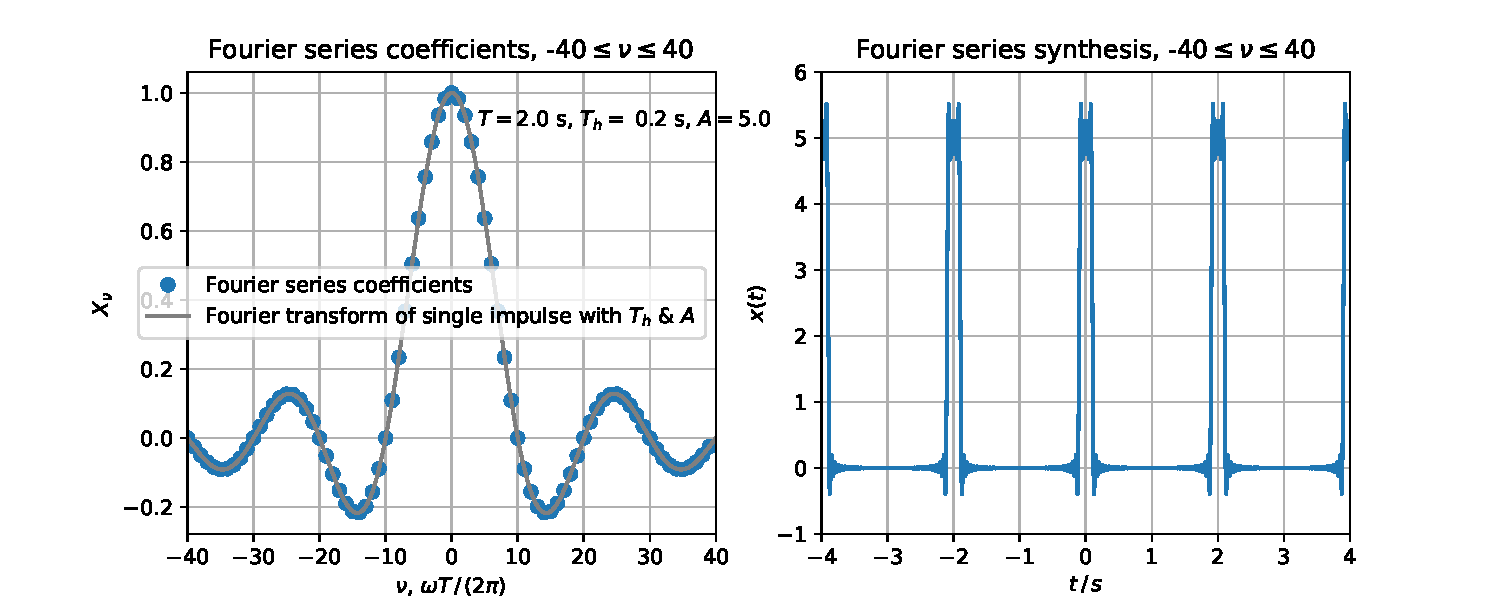
\includegraphics[width=\textwidth]{../fs/D1483A84E2_0.pdf}
\caption{Koeffizienten der komplexen Fourierreihe $X_\nu$ (links) und Synthese $x(t)$ (rechts) für
$T=2$ s, $T_h=0.2$ s, $A=1/T_h$. \texttt{FourierSeries\_D1483A84E2.ipynb}}
\label{fig:D1483A84E2_0}
\end{figure}

\begin{figure}
\includegraphics[width=\textwidth]{../fs/D1483A84E2_1.pdf}
\caption{Koeffizienten der komplexen Fourierreihe $X_\nu$ (links) und Synthese $x(t)$ (rechts) für
$T=2$ s, $T_h=0.4$ s, $A=1/T_h$. \texttt{FourierSeries\_D1483A84E2.ipynb}}
\label{fig:D1483A84E2_1}
\end{figure}

\begin{figure}
\includegraphics[width=\textwidth]{../fs/D1483A84E2_2.pdf}
\caption{Koeffizienten der komplexen Fourierreihe $X_\nu$ (links) und Synthese $x(t)$ (rechts) für
$T=2$ s, $T_h=1$ s, $A=1/T_h$. \texttt{FourierSeries\_D1483A84E2.ipynb}}
\label{fig:D1483A84E2_2}
\end{figure}

\begin{figure}
\includegraphics[width=\textwidth]{../fs/D1483A84E2_3.pdf}
\caption{Koeffizienten der komplexen Fourierreihe $X_\nu$ (links) und Synthese $x(t)$ (rechts) für
$T=2$ s, $T_h=1.6$ s, $A=1/T_h$. \texttt{FourierSeries\_D1483A84E2.ipynb}}
\label{fig:D1483A84E2_3}
\end{figure}

\begin{figure}
\includegraphics[width=\textwidth]{../fs/D1483A84E2_4.pdf}
\caption{Koeffizienten der komplexen Fourierreihe $X_\nu$ (links) und Synthese $x(t)$ (rechts) für
$T=2$ s, $T_h=2$ s, $A=1/T_h$. \texttt{FourierSeries\_D1483A84E2.ipynb}. Extremfall: für die
Darstellung eines Gleichanteils braucht es nur $X_{\nu=0}$, alle anderen Fourier Koeffizienten
$X_{\nu \neq 0}=0$, weil ja nichts schwingt.}
\label{fig:D1483A84E2_4}
\end{figure}











\cleardoublepage
\subsection{Dirac-Impuls}
\label{sec:D410BDAAE0}
\begin{Ziel}
Wir führen den Dirac-Impuls $\delta(t)$ ein.
Ohne den geht in SigSys (fast) nix, bekannt auch als
Dirac-Delta-Impuls, Dirac-Stoß, Einheitsimpuls.
Wir werden den Dirac-Impuls bei der Beschreibung von Signalen und Systemen
in fundamentalen Zusammenhängen benutzen (müssen).
Wir haben mit der vorigen Aufgabe ganz gut vorgearbeitet und können uns
mit der Rechteck- und Spaltfunktion dem Phänomen Dirac-Impuls nähern.
Ingenieur*innen ist das Konzept am Anfang ein wenig fremd, weil
der Dirac-Impuls keine klassische Funktion ist, sondern eine Distribution, d.h.
es gibt bestimmte Funktionen, für die ein eigentlich gewünschter Grenzwert zwar nicht existiert,
die aber gleiche Grundeigenschaften besitzen, wenn man sich dieser Grenze annähert.
Diese Grundeigenschaften werden wir kennenlernen als sehr nützliche
Rechenregeln des Dirac-Impulses, und damit haben wir eigentlich das nötige
Handwerkszeug für SigSys dann schon parat.
Die Rechteck- und Spaltfunktion sind zwei solche Funktionen mit
Grundeigenschaften die einen Dirac-Impuls ausmachen (ganz streng genommen erfüllt
die Rechteckfunktion bestimmte Anforderungen der Distributionstheorie gar nicht,
aber es ist in SigSys-Büchern das deutlich beliebtere Signal einen Dirac Impuls
Grenzübergang aufzuzeigen.)

Zudem werden wir zwei fundamentale Korrespondenzen der Fouriertransformation
kennenlernen, nämlich die des Dirac-Impulses und die des Gleichsignals, das als
weiter Vorgriff auf das was uns erwartet in SigSys.
\end{Ziel}
\textbf{Aufgabe} {\tiny D410BDAAE0}:
Finden Sie $x(t)=\delta(t)\quad \fourier \quad X(\omega)=?$ sowie
$x(t)= ? \quad \fourier \quad X(\omega)=2\pi \delta(\omega)$
\begin{Werkzeug}
Führen wir für $\xi\in\mathbb{N}^+$ eine Funktion $\delta_\xi(t)$ ein, die entweder
\begin{equation}
\delta_\xi(t) := \xi \cdot \mathrm{rect}(\xi \, t) =
\begin{cases} \xi & |t| < \frac{1}{2 \xi} \\ \frac{\xi}{2} & |t| = \frac{1}{2 \xi} \\ 0 & |t| > \frac{1}{2 \xi} \end{cases}\quad
\end{equation}
oder
\begin{equation}
\delta_\xi(t) := \frac{\xi}{\pi} \cdot \mathrm{sinc}(\xi \, t) = \frac{\sin(\xi \, t)}{\pi t}
\end{equation}
ist.
Wir entdecken die---zwar ein wenig normiert aber uns mittlerweile vertraute---
Rechteck- und Spaltfunktion wieder.
%
Es gilt für beide Funktion, und zwar unabhängig von $\xi$ (für die
Rechteckfunktion ist das leicht einzusehen, für die sinc-Funktion überlassen wir
das den Mathematiker*innen und/oder müssen uns vertiefter mit dem Integralsinus
auseinander setzen)
\begin{equation}
\int\limits_{-\infty}^{+\infty} \delta_\xi(t) \fsd t = 1,
\end{equation}
d.h. die \textbf{Fläche ist immer 1} bei der gewählten Normierung der
Rechteck- und Spaltfunktion.
%
Nun sind die Grenzwerte
%\begin{equation}
$\lim_{\xi\to\infty} \delta_\xi(t)$
%\end{equation}
leider nicht definiert, weil die Funktionen wachsen ins Unendliche bei $t=0$.
%
Wir machen uns klar, dass sowohl die Rechteck- als auch Spaltfunktion mit
größer werdendem $\xi\to \infty$ um das Funktionsargument $0$ herum
immer schmaler und höher werden und sich
einem Impuls annähern, siehe \fig{fig:D410BDAAE0}.
%
Die Mathematik\footnote{\url{https://dlmf.nist.gov/1.17} bzw. Bücher wie
\cite[Kapitel 1.11]{Arfken2013}, \cite{Burg2013}}
liefert uns nun eine Lösung im Sinne eines Grenzwerts für eine
Sequenz von Integralen über $\delta_\xi(t)$, $\xi=1,2,3,...$
\begin{equation}
\lim_{\xi\to\infty} \int\limits_{-\infty}^{+\infty}
\delta_\xi(t-t_0) \cdot f(t) \, \fsd t = f(t_0).
\end{equation}
Wir sehen, dass dieser Grenzwert auf eine Funktion $f(t)$ einwirkt und als Lösung
$f(t_0)$ hervorbringt, wenn $\delta_\xi(t)$ um $t_0$ verschoben wurde (der Impuls ist dann bei $t_0$), also
$\delta_\xi(t-t_0)$ im Integral benutzt wurde.
%
Diese Eigenschaft ist das was uns primär in SigSys interessiert.
%
Der für uns etwas sperrige Ausdruck
\begin{equation}
\lim_{\xi\to\infty} \int\limits_{-\infty}^{+\infty}
\delta_\xi(t-t_0) \cdot f(t) \, \fsd t
\end{equation}
bekommt jetzt 'einfach' eine Definition übergeholfen mit
Einführung des sogenannten Dirac-Impulses $\delta(t)$
\begin{equation}
\label{eq:DiracDistrDef}
\lim_{\xi\to\infty} \int\limits_{-\infty}^{+\infty}
\delta_\xi(t-t_0) \cdot f(t) \, \fsd t
:= \int\limits_{-\infty}^{+\infty} \delta(t-t_0) \cdot f(t) \, \fsd t \stackrel{\mathrm{def}}= f(t_0)
\end{equation}
%
Die rechte Seite ist \textbf{kein} klassisches Riemann-Integral, sondern eine
\textbf{Definition} (nämlich die des Grenzwerts für das linke Integral!,
sollte man nicht vergessen, wird aber oft vergessen ;-) ),
für uns aber eine nützliche \text{Rechenregel} und Grundeigenschaft des
Dirac-Impulses. Diese ist als \textbf{Austasteigenschaft} oder
\textbf{Ausblendeigenschaft} (in englisch sifting property, obacht: nicht shifting)
bekannt. Je nachdem wie wir denken wollen:
Austasten nur des Funktionswertes $f(t_0)$ oder Ausblenden aller Funktionswerte
außer $f(t_0)$.

Aus dieser Rechenregel können wir sofort ableiten, dass
\begin{equation}
\label{}
\int\limits_{-\infty}^{+\infty} \delta(t) \cdot f(t) \, \fsd t = f(0)
\end{equation}
wenn $t_0=0$ gewählt wurde.
%
Weiter finden wir
\begin{equation}
\label{eq:D410BDAAE0_area_like}
\int\limits_{-\infty}^{+\infty} \delta(t) \fsd t = 1
\end{equation}
wenn $f(t)=1$ gewählt wurde.
%
Beide Beziehungen konnten wir nur deswegen so schnell und einfach ableiten, weil
wir die Definition benutzt haben. Wir müssen aber immer klar haben, dass wir
nicht das Integral gelöst, sondern vielmehr die Rechenregel der Austastung
verwendet haben.
%
Die Versuchung \eqref{eq:D410BDAAE0_area_like} als Fläche
des Dirac-Impulses zu interpretieren
ist sehr groß, und wenn wir den Grenzübergang mit der Rechteckfunktion in Gedanken
tatsächlich vollziehen auch nicht falsch, aber wir können das streng genommen
nicht aus dem Definitionsintegral (in Notation der Formelsammlung)
$\int\limits_{-\infty}^{+\infty} \delta(t-\tau) \cdot x(t) \, \fsd t \stackrel{\mathrm{def}}= x(\tau)$
des Dirac-Impulses auslesen.
%
Statt Fläche, sprechen wir deswegen zukünftig vom Gewicht 1 des Dirac-Impulses.

\end{Werkzeug}

\noindent Weil es so fundamental wichtig ist, nochmal kompakt für SigSys.
%
Wir stellen uns einen Impuls vor, der
\begin{align}
\int\limits_{t=-\infty}^{+\infty} \delta(t) \fsd t = 1
\qquad\qquad
\delta(t) =
\begin{cases}
\infty & t=0\\
0  & t \neq 0
\end{cases}
\end{align}
als Eigenschaft haben soll. Mit der zweiten Formel kann man aber schlecht rechnen, daher Distribution, Grenzübergang, Definitionsintegral usw., siehe oben.
Am allerwichtigsten ist
\begin{align}
\delta(t) x(t) = \delta(t) x(0)
\end{align}
und dessen Integral
\begin{align}
\int\limits_{t=-\infty}^{+\infty} \delta(t) x(t) \fsd t= \int\limits_{t=-\infty}^{+\infty}  \delta(t) x(0) \fsd t = x(0) \int\limits_{t=-\infty}^{+\infty} \delta(t) \fsd t = x(0),
\end{align}
also die \textbf{Multiplikationseigenschaft} und die \textbf{Austasteigenschaft}.
Wenn man den Impuls verschiebt, so dass die Spitze bei $\tau$ ist, also
\begin{align}
\int\limits_{t=-\infty}^{+\infty} \delta(t-\tau) \fsd t = 1
\qquad\qquad
\delta(t-\tau) =
\begin{cases}
\infty & t=\tau\\
0  & t \neq \tau
\end{cases}
\end{align}
folgt
\begin{align}
\text{Multiplikationseigenschaft allgemein} & \qquad\delta(t-\tau)\,x(t) = \delta(t-\tau)\,x(\tau)\\
\text{Multiplikationseigenschaft für } \tau=0 & \qquad\delta(t)\,x(t) = \delta(t)\,x(0)\\
\text{Austasteigenschaft I allgemein} & \quad \int\limits_{t=-\infty}^{+\infty} \delta(t-\tau) x(t)\fsd t = x(\tau)\\
\text{Austasteigenschaft I für } \tau=0& \quad \int\limits_{t=-\infty}^{+\infty} \delta(t) x(t)\fsd t = x(0)
\end{align}
%
Die allgemeine Austasteigenschaft I können wir mit einem Variablentausch $t \leftrightarrow \tau$ als
\begin{align}
\int\limits_{\tau=-\infty}^{+\infty} \delta(\tau-t) x(\tau)\fsd \tau = x(t)
\end{align}
schreiben. Der Dirac Impuls ist ein gerades Signal, d.h. es gilt $\delta(t)=\delta(-t)$. Es gilt also auch $\delta(\tau-t)=\delta(-(\tau-t))=\delta(-\tau+t)$ und man kann damit die allgemeine Austasteigenschaft II
\begin{align}
\int\limits_{\tau=-\infty}^{+\infty} \delta(-\tau+t) x(\tau)\fsd \tau = x(t),
\end{align}
aufschreiben, die sich auch in der Formelsammlung findet. Typ I und II sind nützlich für verschiedene Rechenwege. Typ I ist in den meisten Lehrbüchern drin und mutmaßlich am Anfang einfacher zu verdauen. Typ II ist sehr gut geeignet, die Faltung elegant herzuleiten.


\begin{figure}[h!]
\includegraphics[width=\textwidth]{../dirac_impulse_ct/D410BDAAE0.pdf}
  \caption{Rechteck- (oben) und normalisierte Spaltfunktion (unten) unterschiedlicher Breite und Höhe.
  Durch die Normierung auf Fläche 1 verhalten sich Breite und Höhe umgekehrt proportional und
  gehen daher in den Grenzfällen zu einem unendlich kleinem Gleichsignal oder einem unendlich kurzen und hohen
  Impuls über. Diese beiden Funktionen gehen im Grenzfall $\xi\to\infty$
  in einen Dirac-Impuls \eq{eq:DiracDistrDef} über.
  \texttt{dirac\_impulse\_CT\_D410BDAAE0.ipynb}}
  \label{fig:D410BDAAE0}
\end{figure}

\begin{figure}[h!]
\centering
%
\begin{tikzpicture}0
\def\l{-2.5}
\def\r{+2.5}
\draw[->] (-2+\l,0) -- (2+\l,0) node[right] {$t$};
\draw[->] (0+\l,0) -- (0+\l,1.5) node[above] {$x(t)=\delta(t)$};
\draw[->, C0, line width=1mm] (0+\l,0) -- (0+\l,1) node[left] {$(1)$};
\node at (0,1) {$\fourier$};
\draw[->] (-2+\r,0) -- (2+\r,0) node[right] {$\omega$};
\draw[->] (0+\r,0) -- (0+\r,1.5) node[above] {$X(\omega)=1$};
\draw[-, C0, line width=1mm] (-2+\r,1) -- (2+\r,1) node[right] {$1$};
\end{tikzpicture}
%
\begin{tikzpicture}0
\def\l{-2.5}
\def\r{+2.5}
\draw[->] (-2+\l,0) -- (2+\l,0) node[right] {$t$};
\draw[->] (0+\l,0) -- (0+\l,1.5) node[above] {$x(t)=1$};
\draw[-, C0, line width=1mm] (-2+\l,1) node[left] {$1$} -- (2+\l,1);
\node at (0,1) {$\fourier$};
\draw[->] (-2+\r,0) -- (2+\r,0) node[right] {$\omega$};
\draw[->] (0+\r,0) -- (0+\r,1.5) node[above] {$X(\omega)=2\pi\delta(\omega)$};
\draw[->, C0, line width=1mm] (0+\r,0) -- (0+\r,1) node[right] {$(2\pi)$};
\end{tikzpicture}
%
\caption{Korrespondenzen Fouriertransformation: \eq{eq:D410BDAAE0_Loesung1} (oben),
\eq{eq:D410BDAAE0_Loesung2} (unten).}
\label{fig:D410BDAAE0_Korrespondenzen}
\end{figure}



\cleardoublepage
\begin{Ansatz}
Die gesuchte Korrespondenz $x(t)=\delta(t)\quad \fourier \quad X(\omega)=?$
können wir ableiten aus der Ausblendeigenschaft
$\int\limits_{-\infty}^{+\infty} \delta(t-t_0) \cdot f(t) \, \fsd t \stackrel{\mathrm{def}}= f(t_0)$
mit $f(t) = \e^{-\im \omega t}$ und $t_0=0$.
%
Dann bekommt die Ausblendeigenschaft das Aussehen der Fouriertransformation
des Dirac-Impulses
\begin{equation}
X(\omega) = \int\limits_{-\infty}^{+\infty} \delta(t) \cdot \e^{-\im \omega t} \, \fsd t \stackrel{\mathrm{def}}= \e^{-\im \omega \cdot 0} = 1
\end{equation}

Auch die gesuchte Korrespondenz
$x(t)= ? \quad \fourier \quad X(\omega)=2\pi \delta(\omega)$ lässt sich
ableiten aus der Ausblendeigenschaft, diesmal mit der Funktionsvariablen Kreisfrequenz, also mit

$\int\limits_{-\infty}^{+\infty} \delta(\omega-\omega_0) \cdot f(\omega) \, \fsd \omega \stackrel{\mathrm{def}}= f(\omega_0)$
für $f(\omega) = \e^{+\im \omega t}$ (Vorzeichen der inversen Fouriertransformation ist $+$!) und $\omega_0=0$.
%
Dann bekommen wir
\begin{equation}
2\pi \cdot \int\limits_{-\infty}^{+\infty} \delta(\omega) \cdot \e^{+\im \omega t} \, \fsd \omega \stackrel{\mathrm{def}}= 2\pi \cdot \e^{+\im \omega \cdot 0} = 2\pi
\end{equation}
%
Weil bei der inversen Fouriertransformation
\begin{align}
x(t) = \frac{1}{2\pi} \int\limits_{-\infty}^{+\infty} X(\omega) \, \e^{+\im \omega t} \fsd \omega
\end{align}
noch der Faktor $\frac{1}{2\pi}$ berücksichtigt werden muss, erhalten wir
\begin{equation}
x(t) = \int\limits_{-\infty}^{+\infty} \delta(\omega) \cdot \e^{+\im \omega t} \, \fsd \omega \stackrel{\mathrm{def}}= \e^{+\im \omega \cdot 0} = 1
\end{equation}

\end{Ansatz}
%\begin{ExCalc}
%\end{ExCalc}
\begin{Loesung}
Damit haben wir zwei weitere wichtige Korrespondenzen gefunden, in der Formelsammlung
ganz oben auf der Liste:
\begin{align}
\label{eq:D410BDAAE0_Loesung1}
x(t)= \delta(t) &\quad \fourier \quad X(\omega)=1\\
\label{eq:D410BDAAE0_Loesung2}
x(t)= 1 &\quad \fourier \quad X(\omega)=2\pi \delta(\omega)\qquad \text{Dirac mit Gewicht}\,\,2\pi
\end{align}
%
Diese sind in \fig{fig:D410BDAAE0_Korrespondenzen} veranschaulicht.
%
Wesentlich ist, dass ein Dirac-Impuls alle Frequenzen gleich gewichtet enthält
(\fig{fig:D410BDAAE0_Korrespondenzen} oben)
und dass ein Gleichsignal, im Spektrum nur einen Dirac-Impuls bei $\omega=0$ enthält
(\fig{fig:D410BDAAE0_Korrespondenzen} unten).
Weil hier eben nichts schwingt, gibt es nur diesen einen Dirac im Spektrum, welcher den
Gleichanteil repräsentiert.
\end{Loesung}




\begin{mdframed}
\textit{Ausblick:}
%
\\\noindent
Wir haben bisher die Korrespondenzen
\begin{align}
x(t)= \delta(t) &\quad \fourier \quad X(\omega)=1\\
x(t)= 1 &\quad \fourier \quad X(\omega)=2\pi \delta(\omega)\\
x(t - \tau) & \quad \fourier \quad X(\omega) \cdot \e^{-\im\omega \tau}\\
x(t) \cdot \e^{+\im\omega_0 t} & \quad \fourier \quad X(\omega-\omega_0)
\end{align}
kennengelernt.
%
Diese lassen sich nun sinnvoll kombinieren, um weitere Korrespondenzen zu finden,
z.B. ein verschobener Dirac-Impuls im Zeitbereich
\begin{align}
\delta(t-\tau)& \quad \fourier \quad 1 \cdot \e^{-\im\omega \tau}.
\end{align}
Das wird uns in SigSys begleiten: Zeitverschiebung führt zu Phasenänderung im Frequenzbereich.

Oder ein verschobener Dirac-Impuls im Frequenzbereich
\begin{align}
1 \cdot \e^{+\im\omega_0 t} & \quad \fourier \quad 2\pi\delta(\omega-\omega_0),
\end{align}
bedeutet Phasenänderung im Zeitbereich, speziell resultiert eine Multiplikation
mit einer komplexen Schwingung auf das ursprüngliche Gleichsignal $x(t)=1$.
%
In der nächsten Übung wird diese Korrespondenz nochmal näher mit einem
Rechteckzeitsignal beleuchtet. Aus der zeitlichen Begrenzung des Gleichsignals
zum Rechtecksignal resultiert ein Übergang vom Dirac-Impuls zur Spaltfunktion
für die Fouriertransformierte.
\end{mdframed}














\newpage
\subsection{Lineare Differentialgleichungen}
\label{sec:A7BEE9E24E}
%
Zunächst keine Aufgabe, sondern erst ein Ausblick in den Kontext einer mutmaßlichen Wiederholung
gestellt.
Wir betrachten hier einleitend den \textbf{SigSys-Teil: Systemanalyse und -synthese}.
Dafür werden wir die Laplace-Transformation (für zeitkontinuierliche Signale, Systeme)
und die $z$-Transformation (für zeitdiskrete Signale/Systeme) kennenlernen, um
Differentialgleichungen und Differenzengleichungen elegant(er) lösbar zu machen.
%
Signale und Systeme sind natürlich sehr eng verknüpft, die hier aufgespannte
Trennung in Signalanalyse/-synthese vs. Systemanalyse/-synthese
sollten wir daher nicht dogmatisch verfolgen, sondern sie dient als grober
Überblick, was uns in SigSys erwarten wird.

In Mathe haben wir das Konzept der Differentialgleichung (DGL) kennengelernt.
%
Wir haben verschiedene Lösungsmöglichkeiten kennengelernt (Variation
der Konstanten, Variablentrennung, Eigenlösungen und charakteristisches Polynom,
Störgliedansätze, usw.). Erschien uns vielleicht ziemlich wirr, weil rechnen
ja, verstehen eher hm...ja/nein/vielleicht?
Das Buch \cite{Strang2014} und andere von Gilbert Strang
lohnt sich durchzuarbeiten; auch die MIT OCW Vorlesungen von ihm sind sehr zu empfehlen.


Lineare DGL mit konstanten (also \textbf{nicht zeitveränderliche}n) Koeffizienten der
ersten und zweiten Ordnung sind die wichtigsten Vertreter, die wir in SigSys
zunächst brauchen, weil man damit beeindruckend viele Dinge bauen und modellieren
kann, Feder-Masse-Dämpfer und RLC-Schwingkreis sind die beiden Klassiker.
%
In den Grundlagen der E-Technik lernten wir alles erst zu Fuß zu lösen, also
die Wechselstromtechnik und die Einschaltvorgänge an RLC-Schaltungen.
%
Nachrichtentechniker*innen bauen sich aus diesen DGLs sogenannte Filter,
früher analog, heute digital.
%
Regelungstechniker*innen bauen sich im Grunde die gleichen Filter, nennen sie nur
selten Filter, sondern eher Glieder mit z.B. differenzierendem, proportionalem,
integrierendem, usw. Verhalten und bauen dann gerne Systeme mit
Rückkopplungsschleifen, weil sie was regeln wollen.
%
Die Brücke zwischen E-Technik und Nachrichten-/Regelungstechnik (und auch
ganz vielen anderen Disziplinen in denen wir mit Signalen agieren...also
auch Energietechnik und Leistungselektronik, Wellentheorie wie
Akustik, Optik, Hochfrequenztechnik usw.) ist SigSys!

Wir werden uns daher in der SigSys einen eleganten Formalismus erarbeiten,
diesen DGL-Typ für beliebige Störgliedansätze zu lösen (am Ende des Tages
müssen wir ja praktisch vorkommende Signale verarbeiten und können uns nicht
auf schicke, auf Papier lösbare Störgliedformeln beschränken)
und das Konzept der Eigenlösungen und des charakteristischen
Polynoms vertiefen bzw. aus anderem Blickwinkel betrachten (am Ende des Tages
wollen wir für eine bestimmte Aufgabe eine Lösung mit gewünschter Genauigkeit
mit dem einfachsten(!) Aufwand erhalten). Praktisch die gesamte SigSys ist daraufhin
ausgelegt, auch wenn sich das momentan noch nicht so anfühlen mag.

Der folgende Abschnitt soll daher die SigSys Denke ein wenig schmackhaft machen und
greift den didaktisch brillanten Faden aus \cite{Strang2014} auf. Viele Dinge
müssten uns aus der Mathe-VL vertraut vorkommen.
%
Zum Auffrischen sei auch \cite{Burg2013} sehr empfohlen, das ist SigSys aus weiterer
Sicht von Mathematiker*innen.
%
\subsubsection{Lineare DGL 2. Ordnung mit konstanten Koeffizienten}
Betrachten wir beispielhaft die lineare DGL 2. Ordnung
\begin{align}
\label{eq:A7BEE9E24E_DGL}
A \frac{\fsd^2 y(t)}{\fsd t^2} + B \frac{\fsd y(t)}{\fsd t} + C y(t) = x(t),
\end{align}
mit den konstanten Koeffizienten $A,B,C\in\mathbb{R}$.
%
Die DGL stellt ein System dar mit dem Eingangssignal $x(t)$
(das ist die Störfunktion / Anregungsfunktion) und dem Ausgangssignal
$y(t)$ (das ist die Lösung der DGL).
%
In der SigSys Literatur ist die Notation von Eingang $x(t)$ und Ausgang $y(t)$
sehr weit verbreitet, aber wir sind gut beraten das im Detail vorher zu checken.
%
Die Koeffizienten $A,B,C$ bestimmen im Wesen, wie das System den Eingang $x(t)$
im Sinne der ersten und zweiten Ableitung \textbf{linear ändert} zum Ausgang $y(t)$.

Die Lösung der DGL ist immer die Superposition von homogener und partikulärer
Lösung
%
\begin{align}
y(t) = y_h(t) + y_p(t)
\end{align}
mit Berücksichtigung der Anfangsbedingungen meist für exakt $t=0$, also gegebenem
$y(0)$, $y'(0)$.
%
Die homogene Lösung findet alle $y_h(t)$ für den Fall $x(t)=0$.
%
Für das spezielle Eingangssignal $x(t)\neq 0$ in
\eq{eq:A7BEE9E24E_DGL} erhalten wir die partikuläre Lösung $y_p(t)$.
%
\subsubsection{Homogene Lösung: Charakteristisches Polynom}
%
Wir haben gelernt (und vielleicht sogar didaktisch fein hergeleitet bekommen,
warum das so sein muss), dass man die homogene Lösung dieser DGL mit dem
Lösungsansatz
\begin{equation}
y_h(t) \propto \e^{\lambda t}\qquad \lambda\in\mathbb{C}
\end{equation}
erhält ($\propto$ meint proportional zu, dann können wir hier erst einmal
eventuelle Vorfaktoren weglassen).
%
Setzen wir diesen Ansatz in \eq{eq:A7BEE9E24E_DGL} ein, führen die Ableitungen
aus, erhalten wir das \textbf{charakteristische Polynom} in der Klammer von
\begin{equation}
(A \lambda^2 + B \lambda + C) \cdot \e^{\lambda t} = 0
\end{equation}
mit den zwei Lösungen ($\e^{\lambda t}$ bekommen wir nicht zu Null)
\begin{align}
\label{eq:A7BEE9E24E_lambdas}
\lambda_{1,2} = \frac{-B \pm \sqrt{B^2-4 A C}}{2 A},
\end{align}
die
\begin{itemize}
  \item a) reell und unterschiedlich sind, wenn $B^2>4 A C$
  \item b) reell und identisch sind, wenn $B^2 = 4 A C$
  \item c) konjugiert-komplex sind, wenn $B^2<4 A C$.
\end{itemize}
%
Für die Fälle a) und c) gilt immer der Ansatz
\begin{mdframed}[backgroundcolor=C3!10]
\begin{align}
\label{eq:A7BEE9E24E_Eigenloesungen}
y_h(t) = c_1 \e^{\lambda_1 t} + c_2 \e^{\lambda_2 t},
\end{align}
\end{mdframed}
%
Wichtig zu erkennen ist, dass wir---je nachdem wie $\lambda_1$ und $\lambda_2$
beschaffen ist (also abhängig von den Koeffizienten $A,B,C$)---verschiedene
Funktionsverläufe als homogene Lösungen erhalten.
Es ginge:
\begin{itemize}
  \item harmonische komplexe, sin- oder cos-Schwingung (wenn $B=0$, d.h. Resonanz)
  \item gedämpfte komplexe, sin- oder cos-Schwingung
  \item aufklingende komplexe, sin- oder cos-Schwingung (in der Praxis zu vermeiden)
  \item abfallender exponentieller Verlauf
  \item ansteigender exponentieller Verlauf (siehe COVID-19, in der Praxis zu vermeiden).
\end{itemize}
Dies sind \textbf{Eigenlösungen} der homogenen DGL und können mit
\eq{eq:A7BEE9E24E_Eigenloesungen} beschrieben werden.
%
Die noch fehlende Eigenlösung für Fall b) ist $y_h(t) = t \e^{\lambda_1 t}$, das
ist der sogenannte aperiodische Grenzfall (auch bekannt als kritisch bedämpfter Fall)
und bedarf deswegen einer eigenständigen Lösung,
den wir hier zunächst mal vernachlässigen wollen.

\subsubsection{Homogene Lösung: Eigenwerte und Vektoren der Koeffizientenmatrix}
%
Es ist bemerkenswert, dass die homogenen Lösungen
auch hervorgehen, wenn man Eigenwerte und Eigenvektoren einer ganz bestimmten Matrix
berechnet. Das ist natürlich kein Zufall; und mit diesem Ansatz können wir viele
nützliche Tools aus der linearen Algebra mitverwenden.

Um die Matrix aufzustellen, schreiben wir zunächst die homogene DGL um zu
\begin{align}
\frac{\fsd^2 y(t)}{\fsd t^2} + \frac{B}{A} \frac{\fsd y(t)}{\fsd t} + \frac{C}{A} y(t) = 0.
\end{align}
%
Wir können diese DGL 2. Ordnung nun auch in zwei getrennten DGL aufschreiben. Das wird
der Grundstein für die Matrix-Sichtweise.
%
Mit den gängigen abgekürzten Schreibweisen für Zeitableitung
\begin{align}
\frac{\fsd y(t)}{\fsd t} = y'(t) = \dot{y}
\end{align}
können wir schreiben
\begin{align}
\frac{\fsd^2 y(t)}{\fsd t^2} = \frac{\fsd y'(t)}{\fsd t} = - \frac{B}{A}  \frac{\fsd y(t)}{\fsd t} - \frac{C}{A}  y(t).
\end{align}
%
Diese beiden Gleichungen können wir nun als einfaches Matrix-Gleichungssystem formulieren
\begin{align}
\label{eq:A7BEE9E24E_uAU}
\vec{u}' = \frac{\fsd}{\fsd t}
\begin{bmatrix}
y(t) \\ y'(t)
\end{bmatrix}
=
\begin{bmatrix}
0 & 1 \\ - \frac{C}{A} & - \frac{B}{A}
\end{bmatrix}
\begin{bmatrix}
y(t) \\ y'(t)
\end{bmatrix}
=
\vec{A} \vec{u}.
\end{align}
%
Wir finden in der Matrix $\vec{A}$ alle Koeffizienten $A,B,C$ wieder, daher
ist es sinnvoll diese als Koeffizientenmatrix zu bezeichnen und sich klarzumachen,
dass diese Matrix das System vollständig beschreibt.

Behauptung:
Dieses Gleichungssystem lässt sich mittels Eigenwert $\lambda$ und passendem
Eigenvektor $\vec{x}$ lösen, also
\begin{align}
\vec{A} \vec{x} = \lambda \vec{x},
\end{align}
wobei es kein Zufall ist, dass wir auch hier die Variable $\lambda$, wie schon
beim charakteristischen Polynom verwenden: es sind die gleichen Zahlen.
Wir wissen, dass man die unbekannten Eigenwerte mittels Ansatz
$(\vec{A} - \lambda \vec{I})\vec{x} = \vec{0}$, also singulärer Matrix
$(\vec{A} - \lambda \vec{I})$, also $\mathrm{det}(\vec{A} - \lambda \vec{I})=0$
findet.
%
Daher
\begin{align}
\vec{A} - \lambda \vec{I} =
\begin{bmatrix}
0 & 1 \\ -\frac{C}{A} & -\frac{B}{A}
\end{bmatrix}
-\lambda
\begin{bmatrix}
1 & 0 \\ 0 & 1
\end{bmatrix}
=
\begin{bmatrix}
-\lambda & 1 \\ -\frac{C}{A} & -\frac{B}{A} - \lambda
\end{bmatrix}
\end{align}
und derer Determinante
\begin{align}
-\lambda \cdot (-\frac{B}{A} - \lambda) - (-\frac{C}{A})\cdot 1 = \lambda^2 + \frac{B}{A} \lambda + \frac{C}{A}.
\end{align}
%
$\mathrm{det}(\vec{A} - \lambda \vec{I})=0$ wird also zu
\begin{align}
A \lambda^2 + B \lambda + C = 0
\end{align}
mit den \textbf{zwei Eigenwerten} $\lambda_{1,2}$ aus \eq{eq:A7BEE9E24E_lambdas},
weil genau nicht zufällig, exakt identisch mit dem charakteristischen Polynom.
%
Für die beiden zugehörigen Eigenvektoren $\vec{x}_{1}$ und $\vec{x}_{2}$ finden sich wegen
dem geforderten
\begin{align}
(\vec{A} - \lambda_{1,2} \vec{I}) \, \vec{x}_{1,2} = \vec{0}
\end{align}
die Lösungen
\begin{align}
\vec{x}_{1,2} =
\begin{bmatrix}
1 \\ \lambda_{1,2}
\end{bmatrix}.
\end{align}
%
Wir schreiben für $\vec{A} \vec{x} = \lambda \vec{x}$
%
\begin{align}
\vec{A}
\begin{bmatrix}
1 \\ \lambda_{1,2}
\end{bmatrix} = \lambda_{1,2}
\begin{bmatrix}
1 \\ \lambda_{1,2}
\end{bmatrix},
\end{align}
%
mit
\begin{align}
\lambda_{1,2} = \frac{-B \pm \sqrt{B^2-4 A C}}{2 A}.
\end{align}
%
Wichtig: das gerade beschriebene Vorgehen funktioniert nur, wenn
$\lambda_1 \neq \lambda_2$, also tatsächlich zwei unabhängige Eigenvektoren vorliegen.
%
$\lambda_1 = \lambda_2$ ist wieder der Spezialfall des aperiodischen Grenzfalls.

Unser Ausgangspunkt war $\vec{A}  \vec{u} = \vec{u}'$ in \eq{eq:A7BEE9E24E_uAU}.
Wie verknüpfen wir das mit der gefundenen Eigenwert/-vektor-Darstellung?
%
Kein stringenter Beweis, aber fundamentale Beobachtung
(weil wir damit das Fundamentalsystem neu erfinden), nämlich
$\frac{\fsd \e^{a t}}{\fsd t} = a \e^{a t}$.
%
Es ist nicht verboten zu erweitern
\begin{align}
\vec{A}
\begin{bmatrix}
1 \\ \lambda_{1,2}
\end{bmatrix}
\e^{\lambda_{1,2} t}
= \lambda_{1,2}
\begin{bmatrix}
1 \\ \lambda_{1,2}
\end{bmatrix}
\e^{\lambda_{1,2} t}
\end{align}
und wir sehen, dass wenn wir
\begin{align}
\vec{u}_{1,2} = \vec{x}_{1,2} \cdot \e^{\lambda_{1,2} t}
\end{align}
definieren, die Gleichung \eq{eq:A7BEE9E24E_uAU} dann aufgeht, weil bei der Ableitung zu
$\vec{u}'_{1,2}$ der benötigte Vorfaktor $\lambda_{1,2}$ entsteht.
%
$\vec{x}_{1,2}$ ist also im Grunde zeitbereinigt, enthält aber als Eigenvektor
alle Informationen, die wir brauchen, um das Systemverhalten zu beschreiben.
%
$\vec{u}_{1,2}$ ist dann die Version, wo die zeitliche Änderung mittels
$\e^{\lambda_{1,2} t}$ berücksichtigt ist.
%
Das gewünschte Gleichungssystem $\vec{u}'=\vec{A}  \vec{u}$ kann nun einfach
gelöst werden:
%
Die Linearkombination aller (hier der beiden) Vektoren $\vec{u}_{1,2}$ ergibt den
Lösungsraum
\begin{mdframed}[backgroundcolor=C3!10]
\begin{align}
\begin{bmatrix}
y(t) \\ y'(t)
\end{bmatrix} =
c_1 \e^{\lambda_1 t}
\begin{bmatrix}
1 \\ \lambda_{1}
\end{bmatrix}
+
c_2 \e^{\lambda_2 t}
\begin{bmatrix}
1 \\ \lambda_{2}
\end{bmatrix},
\end{align}
\end{mdframed}
%
wobei man für die erste Zeile die Lösung $y(t)$ erkennt und für die zweite $y'(t)$
(man erkennt das, aber wir hatten $\vec{u}$ in \eq{eq:A7BEE9E24E_uAU}
eben auch genau so definiert).
%
Wir haben damit die gleiche Lösung der DGL wie beim Rechnen mit dem
charakteristischen Polynom gefunden.
%
Mit dieser homogenen Lösung können wir dann partikuläre Lösungen zum Beispiel mit
Variation der Konstanten berechnen.

Soweit der kurze Abriss mit hoffentlich wiederholendem Charakter.
%
Wir machen weiter mit einem fundamentalen Zusammenhang, der die Grundlage der
SigSys-Theorie für linear Systeme (also lineare DGL mit konstanten Koeffizienten)
ist.
%
Keine Sorge, wenn das folgende ein wenig sperrige Kost ist, es ist mutmaßlich
Neuland, aber der Teaser hier ist wichtig, damit wir ein Gefühl für das Wesen von SigSys
bekommen.

\subsubsection{Spezielle Anregung mit Dirac-Impuls}
\label{sec:Spezielle_Anregung_mit_Dirac_Impuls}
Wir betrachten die homogene Lösung unter einer bestimmten Anfangsbedingung
(vgl. \cite[S.97]{Strang2014})
\begin{align}
A y''(t) + B y'(t) + C y(t) = 0,\quad y(0)=0,\quad y'(0)=\frac{1}{A}.
\end{align}
%
Immer noch nur für $\lambda_1 \neq \lambda_2$ ! wissen wir von oben
\begin{align}
y_h(t) = c_1 \e^{\lambda_1 t} + c_2 \e^{\lambda_2 t},\qquad
y_h'(t) = c_1 \lambda_1 \, \e^{\lambda_1 t} + c_2 \lambda_2 \, \e^{\lambda_2 t}
\end{align}
und mit $y_p=0$ wird für $y=y_h+y_p=y_h$.
Die Anfangsbedingungen berücksichtigt
\begin{align}
y(0) = c_1 + c_2 = 0,\qquad
y'(0) = c_1 \lambda_1 + c_2 \lambda_2 = \frac{1}{A}
\end{align}
Daraus folgt
\begin{equation}
c_1 = -c_2 = \frac{1}{A} \, \frac{1}{\lambda_1 - \lambda_2}
\end{equation}
und diese Koeffizienten eingesetzt
\begin{align}
\label{sec:A7BEE9E24E_hyh}
y(t) =
\frac{1}{A} \, \frac{\e^{\lambda_1 t} - \e^{\lambda_2 t}}{\lambda_1 - \lambda_2}.
\end{align}
%
Soweit, so gut. Schaut aus wie just another Lösung, aber diese hat es in sich:
%

Erinnern wir uns an den Dirac-Impuls aus Aufgabe \ref{sec:D410BDAAE0},
den unendlich hohen und schmalen Impuls,
wofür wir Rechenregeln finden mussten, weil eben keine klassische Funktion.
%
Wenn wir diesen Dirac-Impuls als Anregung / Eingang / Störgröße für unsere DGL
wählen und verschwindende Anfangswerte als linksseitigen Grenzwert
berücksichtigen (ruhendes System bis kurz vor der Anregung bei exakt $t=0$), also

\begin{mdframed}[backgroundcolor=C3!10]
\begin{align}
A y''(t) + B y'(t) + C y(t) = \delta(t),\qquad y'(0_-) = 0,\qquad y(0_-) = 0
\end{align}
\end{mdframed}
erhalten wir als Lösung exakt \eq{sec:A7BEE9E24E_hyh}!
%\begin{align}
%\label{sec:A7BEE9E24E_hyp}
%y(t) =
%\frac{1}{A} \, \frac{\e^{\lambda_1 t} - \e^{\lambda_2 t}}{\lambda_1 - \lambda_2}.
%\end{align}
%
Die Rechnung schauen wir uns zu einem späteren Zeitpunkt an. Es gelingt mit Variation
der Konstanten und Benutzung der Austasteigenschaft des Dirac Impulses,
vgl. \cite[S.133ff]{Strang2014}.
%
Auch das warum schauen wir uns später an. Wir stellen hier zunächst fest, dass:
homogene DGL mit speziellen Anfangsbedingungen zu $t=0$ ist gleich wie
Lösung der Anregung mit Dirac-Impuls $\delta(t)$ zum Zeitpunkt $t=0$ mit
linksseitigen, verschwindenden Anfangsbedingungen.

In SigSys bezeichnen wir diese Lösung als \textbf{Impulsantwort} $h(t)$
eines Systems (das ist die Antwort der Systembeschreibung mittels DGL auf den
Dirac Impuls mit Gewicht 1, Mathematiker*innen
bezeichnen diese Lösung gerne auch als \textbf{Green'sche Funktion})
\begin{mdframed}[backgroundcolor=C3!10]
\begin{align}
h(t) =
\frac{1}{A}\,\frac{\e^{\lambda_1 t} - \e^{\lambda_2 t}}{\lambda_1 - \lambda_2}
\qquad \lambda_1 \neq \lambda_2.
\end{align}
\end{mdframed}

%\newpage
Mit dieser können wir die \textbf{partikuläre Lösung jeder beliebigen Anregung},
also Störfunktion $x(t)$ angeben, und zwar mit dem sogenannten
\textbf{Faltungsintegral} beginnend ab unserem hier gewähltem
Zeitpunkt $t=0$
%
\begin{mdframed}[backgroundcolor=C3!10]
\begin{equation}
y_p(t) = \int\limits_{\tau=0}^{t} h(t-\tau) x(\tau) \fsd \tau
\end{equation}
\end{mdframed}
%
Falls das System vorher in Ruhe war, ist dies auch die komplette Lösung $y(t)$.
%

Wir finden dieses Faltungsintegral (mit allgemeineren Grenzen) in der
Formelsammlung in dem Abschnitt Faltung, da die Operation allgemeingültig als
\textbf{Faltung} bekannt ist.
%
Für einen Zeitpunkt $t$ werden alle Beiträge der Eingangsgröße $x$ mit der Impulsantwort $h$
gewichtet und \textit{addiert}. Bezüglich eines Zeitpunkts $t$, werden \textit{aktuelle}
Eingangswerte $x(t)$ mit dem \textit{Anfang} der Impulsantwort, \textit{lange}
zurückliegende Eingangswerte mit dem \textit{Ende} der Impulsantwort gewichtet.
%
Wir werden das bald im Detail lernen, es ist ein ganz wesentliches Integral und
eine ganz wesentliche Operation und deswegen \textbf{immer klausurrelevant}.
%
Machen wir uns nochmal klar: in $h(t)$ steckt die Systeminformation in Form
der Eigenwerte $\lambda_{1,2}$, also am Ende des Tages in Form der Koeffizienten $A,B,C$.
Die zeitliche Komponente ist durch $\e^{\lambda_{1,2} t}$ abgebildet.

Der hier nicht näher betrachtete aperiodische Grenzfall $\lambda_1 = \lambda_2$
hat eine eigene Impulsantwort $h(t) \propto t \e^{\lambda t}$.
%
Das Faltungsintegral gilt aber konsistent
für alle Fälle a), b), c). Das Integral weiß ja nicht und interessiert sich auch nicht,
dass wir eine Funktion als Impulsantwort auffassen und wir Fallunterscheidungen
vornehmen müssen, je nachdem wie $A$, $B$ und $C$ beschaffen sind.

Wir fragen uns jetzt zu Recht, ob das Faltungsintegral
uns das Leben so viel einfacher macht, als DGLs zu lösen, so wie wir das in Mathe
gelernt haben.
%
Unbedingt ja! Deswegen gehört die SigSys zum Grundausbildungskanon für angehende
Ingenieur*innen.
Es erhellt erstens, was bei DGLs eigentlich passiert, die Rechnerei
ist nicht notwendigerweise einfacher geworden, aber wir werden zweitens mit der
\textbf{Laplace Transformation} eine
Methode kennenlernen diese ganze \textbf{DGL-Rechnerei und Faltungsoperation auf
einfache algebraische Funktionen runterzubrechen}. Aus der Faltung von zwei
Zeitfunktionen wird dann die Multiplikation zweier Laplace Transformierter.
%
Die Laplace Transformierte der Impulsantwort enthält viele Informationen auf
sehr übersichtliche Weise und ist perfekt für die tägliche Ingenieurarbeit, sei
es in der Regelungstechnik, Kommunikationstechnik oder Maschinenbau, Mechatronik.

\newpage
\subsection{Aufgabe: Homogene Lösung einer DGL 2. Ordnung mit konstanten
Koeffizienten und Anfangsbedingungen}
\label{sec:A7BEE9E24E_Aufgabe}
\begin{Ziel}
Anhand eines speziellen (wiederkehrenden) Beispieles, wollen wir die Impulsantwort berechnen. Auch,
wenn wir unsere Lösung jetzt noch nicht anderweitig verifizieren können,
ist es sinnvoll hier nochmal eine DGL zu lösen und dann gleich einen sehr wichtigen
Spezialfall.
\end{Ziel}
\textbf{Aufgabe} {\tiny A7BEE9E24E}: Berechnen Sie für die DGL 2. Ordnung
\begin{align}
\frac{16}{25} \ddot{y}(t) + \frac{24}{25} \dot{y}(t) + y(t) = 0,
\quad \dot{y}(0)=\frac{25}{16}, \quad y(0)=0.
\end{align}
die Lösung $y(t)$ für $t\geq 0$.
\begin{Werkzeug}
Entweder wir benutzen die Sachen aus dem vorangegangen Repetitorium Abschnitt
\ref{sec:A7BEE9E24E} oder
wir befragen unsere Mathe-Vorlesungsunterlagen. Ziel soll zunächst sein, diese
DGL korrekt zu lösen.
\end{Werkzeug}
\begin{Ansatz}
Im github Repository

\url{https://github.com/spatialaudio/signals-and-systems-exercises}

findet sich im Ordner

\verb|tutorial_extended_latex_deu|

im LaTex Skript (pdf liegt im StudIP)

\verb|laplace_transform/laplace_transform_839973EF5D.tex| eine

ausführlichste Lösung.
Dieses Dokument bekommt ab ca. der Mitte des Semesters Relevanz.
\end{Ansatz}
%\begin{ExCalc}
%\end{ExCalc}
\begin{Loesung}
Wir sollten zur Lösung
\begin{align}
y(t) = \frac{25}{16} \e^{-\frac{3}{4} t} \sin(t), \qquad t\geq 0
\end{align}
gelangen.
%
Dies ist eine Sinusschwingung die exponentiell gedämpft wird und mit
$\frac{25}{16}$ gewichtet ist.
Wegen des gestellten Problems haben wir die Impulsantwort dieser DGL berechnet.
\end{Loesung}
  % intro, FS, FT, Dirac, ODE2nd, h(t)

\setcounter{section}{1}
%%------------------------------------------------------------------------------
\newpage
\section{UE 2: Elementarsignale- und Operationen, LTI-System Eigenschaften, Faltung}
\label{sec:ue2_faltung}

Wir müssen uns zunächst mit den zeitkontinuierlichen Elementarsignalen vertraut
machen, siehe \verb|fundamental_signals_CT.pdf| im StudIP unter Formelsammlung.

Diese sind
\begin{itemize}
  \item Exponentialfunktion
  $\e^{s_0 \, t}$ mit $s=\sigma_0 + \im\omega_0, s_0\in\mathbb{C}, \sigma_0\in\mathbb{R}, \omega_0\in\mathbb{R}$
  \item Rechtecksignal $\mathrm{rect}(t)$ (Konvention: Fläche 1)
  \item Dreiecksignal $\mathrm{tri}(t)$  (Konvention: Fläche 1)
  \item Spaltfunktion $\mathrm{sinc}(t):=\frac{\sin t}{t}$
  \item Sprungfunktion $\epsilon(t)$
  \item Vorzeichenfunktion $\mathrm{sgn}(t)$
  \item Dirac Impuls $\delta(t)$
  \item Dirac Impuls Kamm $\Sha$(t)
\end{itemize}
\red{TBD mit tikz / pgfplots}








\newpage
\subsection{Signaloperationen: Verschiebung und Skalierung}
\label{sec:42DE8C69F7}
\begin{Ziel}
Es ist wichtig, dass wir uns für die Zeitfunktion $f(t)$
die Operationen
Zeitverschiebung,
Zeitskalierung und die Amplitudenskalierung, also
$A \cdot f(\left[t-\tau\right]\cdot \theta)$ mit $A,\tau,\theta\in\mathbb{R}$
klarmachen.
%
Wie man so schön sagt, müssen wir das für SigSys im Schlaf beherrschen.
\end{Ziel}
\textbf{Aufgabe} {\tiny 42DE8C69F7}: Stellen Sie
{$x(t) = \frac{3}{4} \cdot \mathrm{rect}(\frac{1}{3} t-\frac{1}{2})$}
grafisch dar.
\begin{Werkzeug}
Für
\begin{equation}
A \cdot f(\left[t-\tau\right]\cdot \theta)  \qquad A,\tau,\theta\in\mathbb{R}
\end{equation}
gilt
\begin{itemize}
  \item Zeitverschiebung mit
  $\tau$: für $\tau>0$ verzögert, rechtsverschoben; für $\tau<0$ vorauseilend, linksverschoben
  \item Zeitskalierung mit $\theta$: für $\theta>1$ Stauchung; für $0<\theta<1$ Streckung
  \item Amplitudenskalierung mit $A$: für $0<|A|<1$ Stauchung, für $|A|>1$ Streckung
  \item (für $A<0$ zusätzlich noch Invertieren der Signalpolarität)
  \item (für $\theta<0$ zusätzlich noch Invertieren des Zeitverlaufs)
\end{itemize}
\end{Werkzeug}
\begin{Ansatz}
Es ist sinnvoll, das Signal in die Darstellung
\begin{equation}
x(t) = \frac{3}{4} \cdot \mathrm{rect}(\left[t-\frac{3}{2}\right]\cdot \frac{1}{3})
\end{equation}
umzuformen, weil dann $t$ ohne Vorfaktor und so wie obige Formel.
Dann lässt sich Zeitverschiebung und Zeitskalierung
getrennt und nacheinander abarbeiten. Hier also zunächst Zeitverzögerung um
$\frac{3}{2}$ und dann zeitliche Streckung (das Signal wird 'langsamer' bzw.
braucht über die Zeit länger) mit $\frac{1}{3}$.
%
Zum Schluss noch die Amplitudenstauchung auf Amplitude $1 \cdot \frac{3}{4}$.
%
Es ist empfehlenswert, sich das kochrezeptartig anzugewöhnen, bis es sitzt.

Bei einem cos()-Signal leuchtet uns die zeitliche Streckung, Stauchung vielleicht
intuitiv ein: ausgehend von $\cos(t)$ schwingt $\cos(2\,t)$ schneller, das ist eine
zeitliche Stauchung.
%
Jedoch ausgehend von $\cos(t)$ schwingt $\cos(\frac{1}{2}\,t)$
langsamer, das ist dann eine zeitliche Streckung.

Machen wir uns klar, dass wir auch eine Verschiebung des Signals bezüglich der
Ordinate vornehmen können. Das heißt wir manipulieren den Gleichanteil.
%
Signale mit Gleichanteil werden in den meisten signallastigen
Ingenieursdisziplinen vermieden, weil man den Gleichanteil schlecht
(elektrische Dauerlast, Wärme) oder gar nicht (z.B. Gleichstrom über Luft?!)
übertragen kann.
%
Wir benutzen das daher in den SigSys-UE seltener.

\end{Ansatz}
%\begin{ExCalc}
%\end{ExCalc}
\begin{Loesung}
Das Signal ist in \fig{fig:42DE8C69F7}d dargestellt. Der Lösungsweg folgt von
\fig{fig:42DE8C69F7}a zu \fig{fig:42DE8C69F7}d.

Eine gute Kontrollmöglichkeit bietet Wolfram Alpha
\url{https://www.wolframalpha.com/}.
Nachdem wir uns vergewissert haben, dass die Rechteckfunktion dort ähnlich definiert
ist (Breite, Höhe, Fläche ist jeweils 1), können wir
\verb|3/4*rect(1/3*t-1/2)| eingeben und bekommen eine analytische und grafische
Lösung von Wolfram Alpha angeboten.
Hinweis: die Sprungfunktion erhalten wir mit \verb|step(t)|
und die Dreieckfunktion mit \verb|tri(t)|, damit können wir eigene einfache
Experimente zur Signalskalierung und -verschiebung machen.
%
Das sollten wir in jedem Fall mal machen in einer Mußestunde!

%Mit UE 1.1 aus dem SS2019 können wir noch mehr üben.
\end{Loesung}

\begin{figure*}[h!]
\centering
\begin{subfigure}{0.45\textwidth}
\begin{tikzpicture}
\begin{axis}[
width=1\textwidth,
height=0.5\textwidth,
domain=-4:4,
samples=50,
legend pos=outer north east,
xlabel = {t},
%ylabel = {x(t)},
title = {$x(t) = \mathrm{rect}(t)$},
xmin=-4, xmax=4,
ymin=-0.1, ymax=1.1,
xtick={-4,-3,-2,-1,0,1,2,3,4},
ytick={0,0.5,1,1.5,2},
ymajorgrids=true,
xmajorgrids=true
]
\addplot[mark=None, color=C0, ultra thick]
coordinates {(-4,0)(-1/2,0)(-1/2,1)(1/2,1)(1/2,0)(4,0)};
\end{axis}
\end{tikzpicture}
\caption{Elementarsignal Rechteckfunktion.}
%\label{fig:}
\end{subfigure}
%
\begin{subfigure}{0.45\textwidth}
\begin{tikzpicture}
\begin{axis}[
width=1\textwidth,
height=0.5\textwidth,
domain=-4:4,
samples=50,
legend pos=outer north east,
xlabel = {t},
%ylabel = {x(t)},
title = {$x(t) = \mathrm{rect}(t-\frac{3}{2})$},
xmin=-4, xmax=4,
ymin=-0.1, ymax=1.1,
xtick={-4,-3,-2,-1,0,1,2,3,4},
ytick={0,0.5,1,1.5,2},
ymajorgrids=true,
xmajorgrids=true
]
\addplot[mark=None, color=C0, ultra thick]
coordinates {(-4,0)(1,0)(1,1)(2,1)(2,0)(4,0)};
\end{axis}
\end{tikzpicture}
\caption{Zeit\textbf{verzögerung}.}
%\label{fig:}
\end{subfigure}


\begin{subfigure}{0.45\textwidth}
\begin{tikzpicture}
\begin{axis}[
width=1\textwidth,
height=0.5\textwidth,
domain=-4:4,
samples=50,
legend pos=outer north east,
xlabel = {t},
%ylabel = {x(t)},
title = {$x(t) = \mathrm{rect}(\left[t-\frac{3}{2}\right]\cdot \frac{1}{3}) = \mathrm{rect}( \frac{t}{3} - \frac{1}{2})$},
xmin=-4, xmax=4,
ymin=-0.1, ymax=1.1,
xtick={-4,-3,-2,-1,0,1,2,3,4},
ytick={0,0.5,1,1.5,2},
ymajorgrids=true,
xmajorgrids=true
]
\addplot[mark=None, color=C0, ultra thick]
coordinates {(-4,0)(0,0)(0,1)(3,1)(3,0)(4,0)};
\end{axis}
\end{tikzpicture}
\caption{Zeitverzögerung und -\textbf{streckung}.}
%\label{fig:}
\end{subfigure}
%
\begin{subfigure}{0.45\textwidth}
\begin{tikzpicture}
\begin{axis}[
width=1\textwidth,
height=0.5\textwidth,
domain=-4:4,
samples=50,
legend pos=outer north east,
xlabel = {t},
%ylabel = {x(t)},
title = {$x(t) = \frac{3}{4} \cdot \mathrm{rect}(\left[t-\frac{3}{2}\right]\cdot \frac{1}{3})$},
xmin=-4, xmax=4,
ymin=-0.1, ymax=1.1,
xtick={-4,-3,-2,-1,0,1,2,3,4},
ytick={0,0.5,1,1.5,2},
ymajorgrids=true,
xmajorgrids=true
]
\addplot[mark=None, color=C0, ultra thick]
coordinates {(-4,0)(0,0)(0,3/4)(3,3/4)(3,0)(4,0)};
\end{axis}
\end{tikzpicture}
\caption{Zeitverzögerung/-streckung, \textbf{Amplitudenstauchung}.}
%\label{fig:}
\end{subfigure}
%
%
%
\caption{Skizzenfahrplan für Aufgabe \ref{sec:42DE8C69F7}.
\red{TBD: ipnyb}}
\label{fig:42DE8C69F7}
\end{figure*}





\newpage
\subsection{Ableitung eines Cosinus-Signalausschnitts}
\label{sec:114F06AFAA}
\begin{Ziel}
Wir wollen ein paar prototypische
Rechenmuster der SigSys kennenlernen. Dabei begegnen uns neben ganz normalem
Mathematik-Tools ein paar SigSys-Eigenheiten, die wir in den ersten Vorlesungen und Übungen
erarbeiten, also Standardsignale und deren Zusammenhänge und Eigenschaften.
\end{Ziel}
\textbf{Aufgabe} {\tiny 114F06AFAA}:
Gegeben ist das skizzierte Signal $x(t)$. Finden Sie einen analytisch geschlossenen
Ausdruck für $x(t)$ mit Hilfe von Elementarsignalen. Berechnen Sie die zeitliche
Ableitung $x'(t)$ und stellen Sie diese grafisch dar.
\begin{center}
\begin{tikzpicture}[scale=0.8]
\def \xmin {-4}
\def \xmax {4.2}
\def \ymin {-1}
\def \ymax {1.5}
\draw[->] (\xmin-0.1 ,0) -- (\xmax+0.1,0) node[below]{$t$};
\draw[->] (0,\ymin-0.1) -- (0,\ymax+0.1) node[left]{$x(t)$};
\foreach \x in {\xmin,...,3}{\draw (\x,0.05) -- (\x,-0.05);}
\draw (0.05,-1) -- (-0.05,-1);
\draw (0.05,1) -- (-0.05,1) node[left]{\small $1$};
\draw(2,0) node[below]{\small $2$};
\begin{scope}
\draw[C0, ultra thick, domain=-2:2,variable=\t,samples=100,smooth] plot(\t,{ cos (4*pi*\t r)});
\draw[C0, ultra thick] (-4,0) -- (-2,0);
\draw[C0, ultra thick] (2,0) -- (4,0);
\draw[C0, dashed, thin] (2,0) -- (2,1);
\draw[C0, dashed, thin] (-2,0) -- (-2,1);
\end{scope}
\end{tikzpicture}
\end{center}

\begin{Werkzeug}
Rechteckfunktion, Skalierung, Zerlegung in Sprungfunktionen, Ableitung

Ausblendeigenschaft / Austasteigenschaft des Dirac-Impulses,
was ja eigentlich eher eine Definition, anstatt eine Eigenschaft ist (siehe Übung~\ref{sec:ue1_intro} (1))
\begin{equation}
\int\limits_{-\infty}^{+\infty} \delta(t-\tau) \cdot f(t) \, \fsd t \stackrel{\mathrm{def}}= f(\tau)
\end{equation}

Multiplikationseigenschaft des Dirac-Impulses
\begin{align}
&\delta(t-\tau) f(t) = \delta(t-\tau) f(\tau)\\
&\delta(t) f(t) = \delta(t) f(0) \qquad \text{speziell für} \qquad \tau=0
\end{align}

\end{Werkzeug}
\begin{Ansatz}
Typische SigSys-Denke: Zeitlich begrenzten Cosinus herstellen indem wir mit der
Rechteckfunktion einen Teil ausschneiden. Dann Mathematik betreiben.
\end{Ansatz}
\begin{ExCalc}
Vier Schwingungen pro 2 Sekunden, also Frequenz $f=2$ Hz, also Kreisfrequenz
$\omega=2\pi\cdot 2 = 4\pi$ rad/s, also $\cos(4\pi t)$ (wir haben zeitlich gestaucht)
der nur zwischen $-2 < t < +2$ schwingt. Wir können den Cos dafür mit einer
geeigneten Rechteckfunktion multiplizieren.

Die benötigte Rechteckfunktion muss axialsymmetrisch sein, d.h. es ist keine
Zeitverschiebung involviert.
Die benötigte Rechteckfunktion muss breiter sein, als das Standardsignal
$\mathrm{rect}(t)$, d.h. es ist eine zeitliche Streckung erforderlich.
Breite von $\mathrm{rect}(t)$ ist 1 (hat auch Fläche 1!), wir brauchen aber
Breite 4, daher $\mathrm{rect}(t\cdot \frac{1}{4})$ (zur Erinnerung:
die Funktion soll sich bei Streckung langsamer über der Zeit ändern, daher
Skalierungsfaktor kleiner 1)

Daher kann das Signal als
\begin{align}
x(t) = \cos(4\pi t) \cdot \mathrm{rect}(\frac{t}{4})\\
\end{align}
darstellt werden. Kurzer Check bei Wolfram Alpha bestätigt, dass wir richtig
gerechnet haben.

Für die Zeitableitung
\begin{align}
\frac{\fsd }{\fsd t} x(t) =
\frac{\fsd }{\fsd t} \cos(4\pi t) \cdot \mathrm{rect}(\frac{t}{4})\\
\end{align}
benötigen wir nun die Produkt- und Kettenregel, sowie die Ableitung des Rechtecksignals.

Wir können das Rechtecksignal als Überlagerung von zwei Sprungfunktionen darstellen,
nämlich
\begin{equation}
\mathrm{rect}(\frac{t}{4}) = \epsilon(t+2) -\epsilon(t-2),
\end{equation}
was in der Grafik unten visualisiert ist. Zu besseren Übersichtlichkeit wurden die
Funktionen minimal verschoben/skaliert, damit wir auch bei eigentlicher
Überlappung sehen, wie sie verlaufen. Das Prinzip sollte erkennbar sein.
%
\begin{center}
\begin{tikzpicture}
\begin{axis}[
width=0.5\textwidth,
height=0.3\textwidth,
domain=-4:4,
samples=50,
legend pos=outer north east,
xlabel = {t},
%ylabel = {x(t)},
title = {Rechteckfunktion aus zwei Sprungfunktionen},
xmin=-4, xmax=4,
ymin=-1.1, ymax=1.1,
xtick={-4,-3,-2,-1,0,1,2,3,4},
ytick={-1,-0.5,0,0.5,1},
ymajorgrids=true,
xmajorgrids=true
]
\addplot[mark=None, color=C1, ultra thick]
coordinates {(-4,0.05)(-2,0.05)(-2,1)(4,1)};
\addplot[mark=None, color=C2, ultra thick]
coordinates {(-4,-0.05)(2,-0.05)(2,-1)(4,-1)};
\addplot[mark=None, color=C0, ultra thick]
coordinates {(-4,0)(-1.95,0)(-1.95,0.95)(2,0.95)(2,0)(4,0)};
\legend{$+\epsilon(t+2)$ (vorauseilend),$-\epsilon(t-2)$ (verzögert),$+\epsilon(t+2)-\epsilon(t-2)=\mathrm{rect}(t\cdot\frac{1}{4})$}
\end{axis}
\end{tikzpicture}
\end{center}

Nun brauchen wir folgende wichtige Erkenntnis (die nur indirekt in der Formelsammlung
steht, nämlich bei den Korrespondenzen zur Laplace Transformation) und in
\fig{fig:114F06AFAA} veranschaulicht ist
\begin{equation}
  \epsilon(t)' = \delta(t)
\end{equation}

Damit können wir jetzt ableiten.

Also, zunächst die Zerlegung der Rechteckfunktion in zwei Sprungfunktionen
\begin{align}
\frac{\fsd }{\fsd t} x(t) =
\frac{\fsd }{\fsd t} \cos(4\pi t) \cdot \left( \epsilon(t+2) -\epsilon(t-2)\right)=\\
\frac{\fsd }{\fsd t} \cos(4\pi t) \epsilon(t+2)
- \frac{\fsd }{\fsd t} \cos(4\pi t) \epsilon(t-2)
\end{align}

Ausformulieren bringt
\begin{align}x'(t)=
+ \cos(4\pi t)' \epsilon(t+2) + \cos(4\pi t) \epsilon(t+2)'
- \cos(4\pi t)' \epsilon(t-2) - \cos(4\pi t) \epsilon(t-2)'
\end{align}
\begin{align}x'(t)=
- 4\pi\sin(4\pi t) \epsilon(t+2) + \cos(4\pi t) \delta(t+2)
+ 4\pi\sin(4\pi t) \epsilon(t-2) - \cos(4\pi t) \delta(t-2)
\end{align}
Umsortieren, damit wir aus den Sprüngen wieder eine Rechteckfunktion machen können
(was natürlich nicht immer geht, hier aber zum Glück, weil...?)
\begin{align}x'(t)=
- 4\pi\sin(4\pi t) (\epsilon(t+2) - \epsilon(t-2))
+ \cos(4\pi t) \delta(t+2)
- \cos(4\pi t) \delta(t-2)
\end{align}
\begin{align}x'(t)=
- 4\pi\sin(4\pi t) \mathrm{rect}(\frac{t}{4})
+ \cos(4\pi t) \delta(t+2)
- \cos(4\pi t) \delta(t-2)
\end{align}
Mit der Multiplikationseigenschaft des Dirac Impulses
\begin{align}
\delta(t-\tau) f(t) = \delta(t-\tau) f(\tau)
\end{align}
finden wir vereinfachte Ausdrücke
\begin{align}
- \delta(t-2) \cos(4\pi t) = - \delta(t-2) \cos(4\pi \cdot 2) = - \delta(t-2)\\
+ \delta(t+2) \cos(4\pi t) = + \delta(t-(-2)) \cos(4\pi \cdot (-2)) = + \delta(t+2)
\end{align}
und damit wird
\begin{align}x'(t)=
- 4\pi\sin(4\pi t) \mathrm{rect}(\frac{t}{4})
+ \delta(t+2)
- \delta(t-2)
\end{align}
\end{ExCalc}

\begin{figure*}[h!]
\centering
\begin{subfigure}{0.29\textwidth}
\begin{tikzpicture}
\begin{axis}[
width=1\textwidth,
height=1\textwidth,
domain=-2:4,
samples=50,
legend pos=outer north east,
xlabel = {t},
%ylabel = {x(t)},
xmin=-2, xmax=4,
ymin=-0.1, ymax=4,
xtick={-2,-1,0,1,2,3,4},
ytick={0,1,2,3,4},
ymajorgrids=true,
xmajorgrids=true
]
\addplot[mark=None, color=C0, ultra thick]
coordinates {(-2,0)(0,0)(4,4)};
\end{axis}
\end{tikzpicture}
\caption{$t \cdot \epsilon(t)$.}
%\label{fig:}
\end{subfigure}
%
\begin{subfigure}{0.29\textwidth}
\begin{tikzpicture}
\begin{axis}[
width=1\textwidth,
height=1\textwidth,
domain=-2:4,
samples=50,
legend pos=outer north east,
xlabel = {t},
%ylabel = {x(t)},
xmin=-2, xmax=4,
ymin=-0.1, ymax=4,
xtick={-2,-1,0,1,2,3,4},
ytick={0,1,2,3,4},
ymajorgrids=true,
xmajorgrids=true
]
\addplot[mark=None, color=C0, ultra thick]
coordinates {(-2,0)(0,0)(0,1)(4,1)};
\end{axis}
\end{tikzpicture}
\caption{Sprungfunktion $\epsilon(t)$.}
%\label{fig:}
\end{subfigure}
%
\begin{subfigure}{0.29\textwidth}
\begin{tikzpicture}
\begin{axis}[
width=1\textwidth,
height=1\textwidth,
domain=-2:4,
samples=50,
legend pos=outer north east,
xlabel = {t},
%ylabel = {x(t)},
xmin=-2, xmax=4,
ymin=-0.1, ymax=4,
xtick={-2,-1,0,1,2,3,4},
ytick={0,1,2,3,4},
ymajorgrids=true,
xmajorgrids=true
]
\addplot[mark=None, color=C0, ultra thick]
coordinates {(0,0)(0,1)};
\addplot[mark=None, color=C0, ultra thick]
coordinates {(-0.2,0.8)(0,1)};
\addplot[mark=None, color=C0, ultra thick]
coordinates {(0.2,0.8)(0,1)};
\node[above] at (200,100) {$(1)$};
\end{axis}
\end{tikzpicture}
\caption{Dirac Impuls $\delta(t)$.}
%\label{fig:}
\end{subfigure}
%
%
%
\caption{Ableitungseigenschaft von links nach rechts: $(t\cdot\epsilon(t))' = \epsilon(t)$,
$\epsilon(t)' = \delta(t)$}
\label{fig:114F06AFAA}
\end{figure*}











\begin{Loesung}

\begin{align}
x(t) = \cos(4\pi t) \cdot \mathrm{rect}(\frac{t}{4})\\
\end{align}

\begin{align}x'(t)=
- 4\pi\sin(4\pi t) \mathrm{rect}(\frac{t}{4})
+ \delta(t+2)
- \delta(t-2)
\end{align}

\begin{center}
\begin{tikzpicture}[scale=0.8]
\def \xmin {-4}
\def \xmax {4.2}
\def \ymin {-1}
\def \ymax {1.5}
\def \scale {0.1}
\draw[->] (\xmin-0.1 ,0) -- (\xmax+0.1,0) node[below]{$t$};
\draw[->] (0,\ymin-0.1) -- (0,\ymax+0.1) node[left]{$x'(t)$};
\foreach \x in {\xmin,...,3}{\draw (\x,0.05) -- (\x,-0.05);}
\draw(2.2,0.5) node[below]{\small $2$};
\draw(2.3,-0.25) node[below]{$(-1)$};
\draw(-2.3,+0.25) node[above]{$(+1)$};
\draw(-1.9,1) node[above]{$4\pi$};
\begin{scope}
\draw[C0, ultra thick,domain=-2:2,variable=\t,samples=100,smooth] plot(\t,{\scale*-4*pi*sin(4*pi*\t r)});
\draw[C0, ultra thick] (-4,0) -- (-2,0);
\draw[C0, ultra thick] (2,0) -- (4,0);
\draw[C0, ultra thick,->] (-2,0) -- (-2,0.5);
\draw[C0, ultra thick,->] (2,0) -- (2,-0.5);
\end{scope}
\end{tikzpicture}
\end{center}

Das Signal $x'(t)$ besteht also aus der Überlagerung des polaritätsinvertierten,
zeitlich begrenzten Sinus (also Sinusimpuls, auch
Sinusburst genannt) und zwei Dirac Impulsen. Im Bild ist die
Polarität des Gewichts per Pfeilrichtung und der Betrag des Gewichts per (1)
indiziert. Also: $-\delta(t-2)$ hat Gewicht $-1$ und ist um die Zeit 2 zeitlich
verzögert,
$+\delta(t+2)$ hat Gewicht $+1$ und ist um Zeit 2 zeitlich vorauseilend.
\end{Loesung}





\newpage
\subsection{Signaloperationen: Zeitverschiebung und Negative Zeitskalierung}
\label{sec:FBE36B0684}
\begin{Ziel}
Es ist wichtig, dass wir uns Zeitverschiebung im Verbund mit negativer Zeitskalierung
als Konzept der Zeitspiegelung bezüglich einer Achse zu einem speziellen Zeitpunkt
klarmachen. Diese Signaloperation ist fundamental wichtig in der Faltung.
\end{Ziel}
\textbf{Aufgabe} {\tiny FBE36B0684}: Stellen Sie die Signale
$x_1(t) = \mathrm{e}^{-t-1} \cdot \epsilon(t+1)$ und
$x_2(t) = \mathrm{e}^{t-2} \cdot \epsilon(-t+2)$
grafisch dar und machen Sie deutlich wie aus Signal $x_1(t)$ mittels Zeitverschiebung
und negativer Zeitskalierung das Signal $x_2(t)$ resultiert.
\begin{Werkzeug}
Wir brauchen die Konzepte (a) der Zeitverschiebung, hier speziell Zeitverzögerung,
also Verschiebung des Signals nach rechts und (b) der Umkehr des Funktionsarguments,
schlampig ausgedrückt, der Zeitumkehr. Letzteres erreichen wir indem wir
für den im Werkzeugkasten aus Aufgabe \ref{sec:42DE8C69F7} definierten
Zeitskalierungsfaktor
$\theta=-1$ zulassen. Wir machen uns klar, dass wir auch andere negative
$\theta$ zulassen könnten, dann wird das Signal nicht nur gespiegelt,
sondern zusätzlich noch gestaucht/gestreckt. Das sollten wir uns mal ganz in Ruhe
mit Wolfram Alpha als Referenzlösung anschauen.
\end{Werkzeug}
\begin{Ansatz}
Es gibt zwei Varianten um von $x_1(t)$ zu $x_2(t)$ zu gelangen:

Variante I: erst Zeitskalierung $\theta=-1$, dann Zeitverschiebung um $\tau$

Variante II: erst Zeitverschiebung um $\tau$, dann Zeitskalierung $\theta=-1$

\end{Ansatz}
\begin{ExCalc}
Mit Wolfram Alpha \url{https://www.wolframalpha.com} können wir uns bei
Unsicherheit Klarheit verschaffen.
%
Ansonsten ist das eine exzellente Gelegenheit für Stift und Papier.
\end{ExCalc}
\begin{Loesung}
Für Variante I siehe \fig{fig:FBE36B0684_1}, für Variante II siehe
\ref{fig:FBE36B0684_2}.

Das Faltungsintegral
\begin{equation}
y(t)
= \int\limits_{-\infty}^{+\infty} x(-\tau+t) h(\tau) \, \fsd \tau
= \int\limits_{-\infty}^{+\infty} x(\tau) h(-\tau+t) \, \fsd \tau
\end{equation}
werden wir in den nächsten Aufgaben benutzen und verstehen.
%
Wir sehen hier, dass genau die hier
diskutierte Zeitverschiebung und negative Zeitskalierung benutzt werden muss, um
die Signaloperationen $x(\tau) \rightarrow x(-\tau+t)$
oder $h(\tau) \rightarrow h(-\tau+t)$ abzubilden.
\textbf{Wir beachten aber}, dass im Faltungsintegral die temporäre Zeitvariable
$\tau$ (das ist keine RC-Glied Zeitkonstante o.ä.) ist und die Zeit $t$
im Ergebnissignal $y(t)$ die Verschiebungsvariable in der Faltung entspricht.
\end{Loesung}

\begin{figure*}[h]
\centering
\begin{subfigure}{0.45\textwidth}
\begin{tikzpicture}
\begin{axis}[
width=1\textwidth,
height=0.45\textwidth,
domain=-1:4,
samples=50,
legend pos=outer north east,
xlabel = {t},
%ylabel = {x(t)},
title = {$x_1(t) = \mathrm{e}^{-\left[t+1\right]} \cdot \epsilon(\left[t+1\right])$},
xmin=-4, xmax=4,
ymin=-0.1, ymax=1.1,
xtick={-4,-3,-2,-1,0,1,2,3,4},
ytick={0,0.5,1,1.5,2},
ymajorgrids=true,
xmajorgrids=true
]
\addplot[mark=None, color=C0, ultra thick]
{exp(-x-1)};
\addplot[mark=None, color=C0, ultra thick]
coordinates {(-4,0)(-1,0)(-1,1)};
\end{axis}
\end{tikzpicture}
\caption{Ausgangspunkt: abfallende, vorauseilende Exponential-Funktion.}
%\label{fig:}
\end{subfigure}
%
\begin{subfigure}{0.45\textwidth}
\begin{tikzpicture}
\begin{axis}[
width=1\textwidth,
height=0.45\textwidth,
domain=-4:-1,
samples=50,
legend pos=outer north east,
xlabel = {t},
%ylabel = {x(t)},
title = {$\mathrm{e}^{+\left[t+1\right]} \cdot \epsilon(-\left[t+1\right])$},
xmin=-4, xmax=4,
ymin=-0.1, ymax=1.1,
xtick={-4,-3,-2,-1,0,1,2,3,4},
ytick={0,0.5,1,1.5,2},
ymajorgrids=true,
xmajorgrids=true
]
\addplot[mark=None, color=C0, ultra thick]
{exp(x+1)};
\addplot[mark=None, color=C0, ultra thick]
coordinates {(-1,1)(-1,0)(4,0)};
\end{axis}
\end{tikzpicture}
\caption{Umkehr der Funktionsargumente von (a) ist Spiegelung an der $t=-1$ Achse.}
%\label{fig:}
\end{subfigure}

\begin{subfigure}{0.45\textwidth}
\begin{tikzpicture}
\begin{axis}[
width=1\textwidth,
height=0.45\textwidth,
domain=-4:2,
samples=50,
legend pos=outer north east,
xlabel = {t},
%ylabel = {x(t)},
title = {$x_2(t) = \mathrm{e}^{(+\left[t+1-3\right])} \cdot \epsilon(-\left[t+1-3\right])$},
xmin=-4, xmax=4,
ymin=-0.1, ymax=1.1,
xtick={-4,-3,-2,-1,0,1,2,3,4},
ytick={0,0.5,1,1.5,2},
ymajorgrids=true,
xmajorgrids=true
]
\addplot[mark=None, color=C0, ultra thick]
{exp(+(x-2))};
\addplot[mark=None, color=C0, ultra thick]
coordinates {(2,1)(2,0)(4,0)};
\end{axis}
\end{tikzpicture}
\caption{Erst Umkehr der Funktionsargumente von (a) und dann Zeitverzögerung von
(b) um $3$.}
%\label{fig:}
\end{subfigure}
%
%
%
\caption{Skizzenfahrplan für Aufgabe \ref{sec:FBE36B0684},
\textbf{zuerst Zeitskalierung $\theta=-1$, dann Zeitverschiebung}.
Vgl. \texttt{TimeMirrorShift\_FBE36B0684.ipynb}}
\label{fig:FBE36B0684_1}
\end{figure*}
%
%
%
\begin{figure*}[h]
\centering
\begin{subfigure}{0.45\textwidth}
\begin{tikzpicture}
\begin{axis}[
width=1\textwidth,
height=0.45\textwidth,
domain=-1:4,
samples=50,
legend pos=outer north east,
xlabel = {t},
%ylabel = {x(t)},
title = {$x_1(t) = \mathrm{e}^{-\left[t+1\right]} \cdot \epsilon(\left[t+1\right])$},
xmin=-4, xmax=4,
ymin=-0.1, ymax=1.1,
xtick={-4,-3,-2,-1,0,1,2,3,4},
ytick={0,0.5,1,1.5,2},
ymajorgrids=true,
xmajorgrids=true
]
\addplot[mark=None, color=C0, ultra thick]
{exp(-(x+1))};
\addplot[mark=None, color=C0, ultra thick]
coordinates {(-4,0)(-1,0)(-1,1)};
\end{axis}
\end{tikzpicture}
\caption{Ausgangspunkt: abfallende, vorauseilende Exponential-Funktion.}
%\label{fig:}
\end{subfigure}
%
\begin{subfigure}{0.45\textwidth}
\begin{tikzpicture}
\begin{axis}[
width=1\textwidth,
height=0.45\textwidth,
domain=2:4,
samples=50,
legend pos=outer north east,
xlabel = {t},
%ylabel = {x(t)},
title = {$\mathrm{e}^{(-\left[t+1-3\right])} \cdot \epsilon(\left[t+1-3\right])$},
xmin=-4, xmax=4,
ymin=-0.1, ymax=1.1,
xtick={-4,-3,-2,-1,0,1,2,3,4},
ytick={0,0.5,1,1.5,2},
ymajorgrids=true,
xmajorgrids=true
]
\addplot[mark=None, color=C0, ultra thick]
{exp(-(x-2))};
\addplot[mark=None, color=C0, ultra thick]
coordinates {(-4,0)(2,0)(2,1)};
\end{axis}
\end{tikzpicture}
\caption{Zeitverzögerung von (a) um $3$.}
%\label{fig:}
\end{subfigure}

\begin{subfigure}{0.45\textwidth}
\begin{tikzpicture}
\begin{axis}[
width=1\textwidth,
height=0.45\textwidth,
domain=-4:2,
samples=50,
legend pos=outer north east,
xlabel = {t},
%ylabel = {x(t)},
title = {$x_2(t) = \mathrm{e}^{(+\left[t+1-3\right])} \cdot \epsilon(-\left[t+1-3\right])$},
xmin=-4, xmax=4,
ymin=-0.1, ymax=1.1,
xtick={-4,-3,-2,-1,0,1,2,3,4},
ytick={0,0.5,1,1.5,2},
ymajorgrids=true,
xmajorgrids=true
]
\addplot[mark=None, color=C0, ultra thick]
{exp(+(x-2))};
\addplot[mark=None, color=C0, ultra thick]
coordinates {(2,1)(2,0)(4,0)};
\end{axis}
\end{tikzpicture}
\caption{Erst Zeitverzögerung von (a) um $3$ und danach Umkehr der Funktionsargumente von (b).
Daher Spiegelung des Signals von (b) an der $t=2$ Achse.}
%\label{fig:}
\end{subfigure}
%
%
%
\caption{Skizzenfahrplan für Aufgabe \ref{sec:FBE36B0684},
\textbf{zuerst Zeitverschiebung, dann Zeitskalierung $\theta=-1$}.
Vgl. \texttt{TimeMirrorShift\_FBE36B0684.ipynb}}
\label{fig:FBE36B0684_2}
\end{figure*}






\clearpage
\subsection{Test auf Linearität und Zeitinvarianz von Systembeschreibungen}
\label{sec:25F7F29E2A}
\begin{Ziel}
Wir wollen bei prototypischen Systembeschreibungen den Test auf
Linearität und Zeitinvarianz durchführen, um ein Gefühl dafür zu entwickeln,
mit welchen Systemen die LTI-Signalverarbeitung operieren darf und mit welchen nicht.
\end{Ziel}
\textbf{Aufgabe} {\tiny 25F7F29E2A}: Testen Sie für die unten gegebenen
Systembeschreibungen, ob Linearität und Zeitinvarianz vorliegt.
Was macht das System? Was wäre ein passender Name für das System?
\begin{Werkzeug}
Folgen wir der Systemoperatorschreibweise
\begin{equation}
y(t) = \sysH{x(t)}
\end{equation}
mit Eingangssignal $x(t)$ in das System $\sysH{}$ und resultierendem
Ausgangssignal $y(t)$.

\textbf{Test auf Linearität}:
%
Ein System ist genau dann linear, wenn für die Superposition und Amplituden-Skalierung
von Signalen
\begin{equation}
\sysH{a\cdot x_1(t) + b\cdot x_2(t)} = a\cdot\sysH{x_1(t)} + b\cdot\sysH{x_2(t)}
\end{equation}
gilt.
Um auf Linearität zu testen, können wir auch die zwei äquivalenten Bedingungen
\begin{align}
\sysH{x_1(t) + x_2(t)} =& \sysH{x_1(t)} + \sysH{x_2(t)} &\text{Addition}\\
\sysH{a \cdot x_1(t)} =& a \cdot \sysH{x_1(t)} &\text{Skalierung}
\end{align}
betrachten.
Das heißt also: Bei einem linearen System ist es egal, ob wir a) Einzelsignale
vorher addieren und dann durch das System schicken oder die Einzelsignale durch das
System schicken und dann die Ausgangssignale addieren \textbf{UND} b)
eine Amplitudenskalierung beim Eingangssignal oder Ausgangssignal vornehmen. Es kommt
das gleiche Ergebnis heraus. Bei einem nichtlinearen System ist mindestens eins dieser
zwei Kriterien verletzt.

\textbf{Test auf Zeitinvarianz}:
Ein System ist genau dann zeitinvariant, wenn für $y(t) = \sysH{x(t)}$,
eine Zeitverschiebung um $\tau$ zu
\begin{align}
y(t-\tau) = \sysH{x(t-\tau)}
\end{align}
führt.
Vielleicht macht das Bild es noch klarer:
Wir müssen ausgehend von $x(t)$ testen, ob
\begin{equation}
\text{Pfad 1:} \quad x(t)\rightarrow x(t-\tau)\rightarrow \mathcal{H}\{x(t-\tau)\}=y(t-\tau)
\end{equation}
zum gleichen Ergebnis führt wie
\begin{equation}
\text{Pfad 2:} \quad x(t)\rightarrow \mathcal{H}\{x(t)\}=y(t)\rightarrow y(t-\tau).
\end{equation}
%
\begin{center}
\begin{tikzpicture}
\matrix (m) [matrix of nodes, row sep=1cm, column sep=1cm]{
\node(x){$x(t)$}; &
\node(y){$y(t)$};\\
\node(xshift){$x(t-\tau)$};&
\node(yshift){$y(t-\tau)$};\\
};
\draw[->] (x) -- node[above]{$\mathcal{H}$} (y);
\draw[->] (xshift) -- node[above]{$\mathcal{H}$} (yshift);
\draw[->] (x) -- node[left]{Zeitverschiebung um $\tau$} (xshift);
\draw[->] (y) -- node[right]{Zeitverschiebung um $\tau$} (yshift);
\end{tikzpicture}
\end{center}
%
Eine Zeitvorauseilung oder -verzögerung auf das Einganssignal hat die gleiche
Zeitvorauseilung oder -verzögerung beim Ausgangssignal zur Folge.
%
Zeitinvarianz nochmal aus anderem Blick:
Ein zeit(verschiebungs)invariantes System verhält sich bezüglich
der Variable Zeit immer gleich, egal ob wir das System gestern, heute oder
morgen oder sonst wann benutzten.
%
Bei Test auf Zeitinvarianz, ist es manchmal eleganter ein einziges Gegenbeispiel
finden zu können, also zu suchen wo prototypisch die geforderte Gleichheit der
Pfade 1 und 2 verletzt wird.

Wenn die Bedingungen für Linearität \textbf{UND} für Zeitinvarianz erfüllt sind, ist das
System linear und zeitinvariant, in Englisch \textbf{linear and time-invariant}, daher die
sehr gebräuchliche Abkürzung \textbf{LTI-System}. Wir werden uns im Laufe der SigSys ausschließlich
mit LTI-Systemen beschäftigen, weil zum Einen viele Systeme in ihren jeweilig
benutzten Arbeitspunkten annähernd LTI-Eigenschaften haben und zum Anderen, weil die
zunächst zu erarbeitenden Werkzeuge noch vergleichsweise einfach sind.
Ohne LTI-Annahme wird SigSys ein sehr komplizierte Welt, was typisch erst in
sehr spezialisierten Masterstudiengängen gelehrt wird.
\end{Werkzeug}


\begin{Ansatz}
Wir sind hier gut beraten, bei Linearität stur die Tests durchzuführen.
Selbst bei einfach aussehenden Systemen kann es nämlich passieren, dass wir mit
einer intuitiven Bauchgefühlslösung falsch liegen.
\end{Ansatz}
\begin{ExCalc}
siehe Abschnitt Lösung
\end{ExCalc}


\begin{Loesung}
\textbf{Test auf Linearität}:
\begin{align}
\sysH{x_1(t) + x_2(t)} =& \sysH{x_1(t)} + \sysH{x_2(t)} &\text{Additionseigenschaft}\\
\sysH{a \cdot x_1(t)} =& a \cdot \sysH{x_1(t)} &\text{Skalierungseigenschaft}
\end{align}

\begin{itemize}
\item  \underline{System 1}:
\begin{equation}
y(t) = \sysH{x(t)}:=2 x(t)
\end{equation}
Additionseigenschaft ok (erste und letzte Zeile in der Formel identisch):
\begin{align}
\sysH{x_1(t)+x_2(t)}=2\,\,\,(x_1(t) + x_2(t))\\
y_{1,2}(t) = \sysH{x_{1,2}(t)}=2 x_{1,2}(t)\\
\sysH{x_1(t)} + \sysH{x_2(t)} = 2 x_1(t) + 2 x_2(t)
\end{align}
Skalierungseigenschaft ok (beide Zeilen identisch, Klammern helfen den hier trivialen
Fall noch offensichtlicher zu machen):
\begin{align}
\sysH{a \cdot x(t)}= 2\,\,\,( a \cdot x(t))\\
a \cdot \sysH{x(t)}=  a \cdot (2 x(t))
\end{align}
\textbf{linear}, Beispiel/Anwendung: idealer Verstärker
%------------------------------------------------------------------------------
\item  \underline{System 2}:
\begin{equation}
y(t) = \sysH{x(t)}:= 2 x(t) + 1
\end{equation}
Additionseigenschaft : nicht ok
\begin{align}
\sysH{x_1(t)+x_2(t)}= 2(x_1(t)+x_2(t)) + 1\\
y_{1,2}(t) = \sysH{x_{1,2}(t)}= 2 x_{1,2}(t) + 1\\
\sysH{x_1(t)} + \sysH{x_2(t)} = 2 x_{1}(t) + 1 + 2 x_{2}(t) + 1
\end{align}
Skalierungseigenschaft : nicht ok
\begin{align}
\sysH{a \cdot x(t)}= a \cdot 2 x(t) + 1\\
a \cdot \sysH{x(t)}= a \cdot (2 x(t) + 1)
\end{align}
\textbf{nicht linear}, Beispiel/Anwendung: Verstärker mit Offset
%------------------------------------------------------------------------------
\item  \underline{System 3}:
\begin{equation}
y(t) = \sysH{x(t)}:= \mathrm{atan}(x(t))
\end{equation}
Additionseigenschaft nicht ok, vgl. Funktionsverlauf der atan-Funktion:
\begin{align}
\sysH{x_1(t)+x_2(t)}=\mathrm{atan}(x_1(t)+x_2(t))\\
y_{1,2}(t) = \sysH{x_{1,2}(t)}= \mathrm{atan}(x_{1,2}(t))\\
\sysH{x_1(t)} + \sysH{x_2(t)} = \mathrm{atan}(x_1(t)) + \mathrm{atan}(x_2(t))
\end{align}
Skalierungseigenschaft nicht ok, hier sogar noch schneller ersichtlich, für
$|a x(t)|>\frac{\pi}{2}$ landen wir im hochgradig nichtlinearen Teil der atan-Funktion
\begin{align}
\sysH{a \cdot x(t)}= \mathrm{atan}(a \cdot x(t))\\
a \cdot \sysH{x(t)}= a \cdot \mathrm{atan}(x(t))
\end{align}
\textbf{nicht linear}, Beispiel/Anwendung: Amplitudenbegrenzer, Verstärkerkennlinie
zwischen Ein- und Ausgang, für die Musiker*innen unter uns: Limiter, Distortion Effekt
%------------------------------------------------------------------------------
\item  \underline{System 4}:
\begin{equation}
y(t) = \sysH{x(t)}:= \mathrm{sgn(x(t))} \, x(t)
\end{equation}
Additionseigenschaft nicht ok, vgl. Funktionsverlauf der sgn-Funktion:
\begin{align}
\sysH{x_1(t)+x_2(t)}=\mathrm{sgn(x_1(t)+x_2(t))} \, (x_1(t)+x_2(t))\\
y_{1,2}(t) = \sysH{x_{1,2}(t)}= \mathrm{sgn(x_{1,2}(t))} \, x_{1,2}(t)\\
\sysH{x_1(t)} + \sysH{x_2(t)} = \mathrm{sgn(x_{1}(t))} \, x_{1}(t) + \mathrm{sgn(x_{2}(t))} \, x_{2}(t)
\end{align}
Skalierungseigenschaft nicht ok: für $a<0$ gibt es keine Gleichheit:
\begin{align}
\sysH{a \cdot x(t)}= \mathrm{sgn( a \cdot x(t))} \, a \cdot x(t)\\
a \cdot \sysH{x(t)}= a \cdot \mathrm{sgn(x(t))} \, x(t)
\end{align}
\textbf{nicht linear}, Beispiel/Anwendung: Gleichrichter
%------------------------------------------------------------------------------
\item  \underline{System 5}:
\begin{equation}
y(t) = \sysH{x(t)}:= x(t) \cos(\omega_0 t)
\end{equation}
Additionseigenschaft ok:
\begin{align}
\sysH{x_1(t)+x_2(t)}=(x_1(t) + x_2(t)) \cos(\omega_0 t)\\
y_{1,2}(t) = \sysH{x_{1,2}(t)}= x_{1,2}(t) \cos(\omega_0 t)\\
\sysH{x_1(t)} + \sysH{x_2(t)} = x_{1}(t) \cos(\omega_0 t) + x_{2}(t) \cos(\omega_0 t)
\end{align}
Skalierungseigenschaft ok:
\begin{align}
\sysH{a \cdot x(t)}= (a \cdot x(t)) \cos(\omega_0 t)\\
a \cdot \sysH{x(t)}= a \cdot (x(t) \cos(\omega_0 t))
\end{align}
\textbf{linear}, Beispiel/Anwendung: Modulator, für die Musiker*innen unter uns:
Chorus, Flanger Effekte, Vibrato, für NTler*innen: Amplitudenmodulation, CB-Funk

%------------------------------------------------------------------------------
\item  \underline{System 6}:
\begin{equation}
y(t) = \sysH{x(t)}:= x(t+1)
\end{equation}
Additionseigenschaft ok:
\begin{align}
\sysH{x_1(t)+x_2(t)} = x_1(t+1) + x_2(t+1)\\
y_{1,2}(t) = \sysH{x_{1,2}(t)}= x_{1,2}(t+1)\\
\sysH{x_1(t)} + \sysH{x_2(t)} = x_1(t+1) + x_2(t+1)
\end{align}
Skalierungseigenschaft ok:
\begin{align}
\sysH{a \cdot x(t)}= a x(t+1)\\
a \cdot \sysH{x(t)}= a x(t+1)
\end{align}
\textbf{linear}, Beispiel/Anwendung: Orakel (zeitlich in die Zukunft schauend)
%------------------------------------------------------------------------------
\item  \underline{System 7}:
\begin{equation}
y(t) = \sysH{x(t)}:= \sum_{m=0}^{10} 2^{-m} x(t-m)
\end{equation}
Additionseigenschaft ok:
\begin{align}
\sysH{x_1(t)+x_2(t)}=\sum_{m=0}^{10} 2^{-m} (x_1(t-m)+x_2(t-m))\\
y_{1,2}(t) = \sysH{x_{1,2}(t)}= \sum_{m=0}^{10} 2^{-m} x_{1,2}(t-m)\\
\sysH{x_1(t)} + \sysH{x_2(t)} = \sum_{m=0}^{10} 2^{-m} x_1(t-m) + \sum_{m=0}^{10} 2^{-m} x_2(t-m)
\end{align}
Skalierungseigenschaft ok:
\begin{align}
\sysH{a \cdot x(t)}= \sum_{m=0}^{10} 2^{-m} a \cdot x(t-m)\\
a \cdot \sysH{x(t)}= a \cdot \sum_{m=0}^{10} 2^{-m} x(t-m)
\end{align}
\textbf{linear}, Beispiel/Anwendung: Echo
%------------------------------------------------------------------------------
\item  \underline{System 8}:
\begin{equation}
y(t) = \sysH{x(t)}:= x(t) + x(-t)
\end{equation}
Additionseigenschaft ok:
\begin{align}
\sysH{x_1(t)+x_2(t)}=(x_1+x_2)(t)+(x_1+x_2)(-t)\\
y_{1,2}(t) = \sysH{x_{1,2}(t)}= x_{1,2}(t)+x_{1,2}(-t)\\
\sysH{x_1(t)} + \sysH{x_2(t)} = x_{1}(t)+x_{1}(-t) + x_{2}(t)+x_{2}(-t)
\end{align}
Skalierungseigenschaft ok:
\begin{align}
\sysH{a \cdot x(t)}= a \cdot x(t) + a \cdot x(-t)\\
a \cdot \sysH{x(t)}= a \cdot (x(t) + x(-t))
\end{align}
\textbf{linear}, Beispiel/Anwendung: 'Gerademacher', oder besser: ungerade
Eingangsfunktionen werden ausgelöscht
%------------------------------------------------------------------------------
\item  \underline{System 9}:
\begin{equation}
y(t) = \sysH{x(t)}:= \frac{\fsd x(t)}{\fsd t} = \frac{\fsd}{\fsd t} \cdot x(t)
\end{equation}
Additionseigenschaft ok:
\begin{align}
\sysH{x_1(t)+x_2(t)}=\frac{\fsd}{\fsd t} (x_1(t)+x_2(t))\\
y_{1,2}(t) = \sysH{x_{1,2}(t)}= \frac{\fsd}{\fsd t} x_{1,2}(t)\\
\sysH{x_1(t)} + \sysH{x_2(t)} = \frac{\fsd}{\fsd t} x_{1}(t) + \frac{\fsd}{\fsd t} x_{2}(t)
\end{align}
Skalierungseigenschaft :
\begin{align}
\sysH{a \cdot x(t)}= \frac{\fsd}{\fsd t}(a \cdot x(t))\\
a \cdot \sysH{x(t)}= a\cdot \frac{\fsd}{\fsd t} x(t)
\end{align}
\textbf{linear}, Ableitungsoperator ist ein linearer Operator!
Beispiel/Anwendung: Differenzierer
%------------------------------------------------------------------------------
\item  \underline{System 10}:
\begin{equation}
y(t) = \sysH{x(t)}:= \int\limits_{-\infty}^{t} x(\tau) \fsd \tau
\end{equation}
Additionseigenschaft ok:
\begin{align}
\sysH{x_1(t)+x_2(t)}= \int\limits_{-\infty}^{t} (x_1(\tau)+x_2(\tau)) \fsd \tau\\
y_{1,2}(t) = \sysH{x_{1,2}(t)}= \int\limits_{-\infty}^{t} x_{1,2}(\tau) \fsd \tau\\
\sysH{x_1(t)} + \sysH{x_2(t)} = \int\limits_{-\infty}^{t} x_1(\tau) \fsd \tau + \int\limits_{-\infty}^{t} x_2(\tau) \fsd \tau
\end{align}
Skalierungseigenschaft ok:
\begin{align}
\sysH{a \cdot x(t)}= \int\limits_{-\infty}^{t} a \cdot x(\tau) \fsd \tau\\
a \cdot \sysH{x(t)}= a \cdot \int\limits_{-\infty}^{t} x(\tau) \fsd \tau
\end{align}
\textbf{linear}, Integrationsoperator ist ein linearer Operator.
Beispiel/Anwendung: Integrierer
%------------------------------------------------------------------------------
\item  \underline{System 11}:
\begin{equation}
y(t) = \sysH{x(t)}:= \int\limits_{-\infty}^{t} |x(\tau)|^2 \fsd \tau
\end{equation}
Hier dürfen wir sogar mal auf unser Bauchgefühl hören: Quadrat und Betrag erlauben
keine Linearität.

Additionseigenschaft nicht ok
\begin{align}
\sysH{x_1(t)+x_2(t)}= \int\limits_{-\infty}^{t} |x_1(\tau)+x_2(\tau)|^2 \fsd \tau\\
y_{1,2}(t) = \sysH{x_{1,2}(t)}= \int\limits_{-\infty}^{t} |x_{1,2}(\tau)|^2 \fsd \tau\\
\sysH{x_1(t)} + \sysH{x_2(t)} = \int\limits_{-\infty}^{t} |x_{1}(\tau)|^2 \fsd \tau+\int\limits_{-\infty}^{t} |x_{2}(\tau)|^2 \fsd \tau
\end{align}
Skalierungseigenschaft nicht ok, Skalierung wirkt vor/nach Quadrierung anders,
speziell auch $a<0$ delikat:
\begin{align}
\sysH{a \cdot x(t)}= \int\limits_{-\infty}^{t} |a \cdot x(\tau)|^2 \fsd \tau\\
a \cdot \sysH{x(t)}= a\cdot \int\limits_{-\infty}^{t} |x(\tau)|^2 \fsd \tau
\end{align}
\textbf{nicht linear}, Beispiel/Anwendung: Energiemesser
%------------------------------------------------------------------------------
\item  \underline{System 12}:
\begin{equation}
y(t) = \sysH{x(t)}:= |x(t)|
\end{equation}
Additionseigenschaft nicht ok:
\begin{align}
\sysH{x_1(t)+x_2(t)}= |x_1(t) + x_2(t)|\\
y_{1,2}(t) = \sysH{x_{1,2}(t)}= |x_{1,2}(t)|\\
\sysH{x_1(t)} + \sysH{x_2(t)} = |x_1(t)| + |x_2(t)|
\end{align}
Skalierungseigenschaft nicht ok (vgl. $a<0$):
\begin{align}
\sysH{a \cdot x(t)}= |a \cdot x(t)|\\
a \cdot \sysH{x(t)}= a \cdot |x(t)|
\end{align}
\textbf{nicht linear}, Gleichrichter

%------------------------------------------------------------------------------
\item  \underline{System 13}:
\begin{equation}
y(t) = \sysH{x(t)}:= x(t) \epsilon(t)
\end{equation}
Additionseigenschaft ok:
\begin{align}
\sysH{x_1(t)+x_2(t)}= (x_1(t) + x_2(t)) \epsilon(t)\\
y_{1,2}(t) = \sysH{x_{1,2}(t)}= x_{1,2}(t)\epsilon(t)\\
\sysH{x_1(t)} + \sysH{x_2(t)} = x_1(t) \epsilon(t) + x_2(t) \epsilon(t)
\end{align}
Skalierungseigenschaft ok:
\begin{align}
\sysH{a \cdot x(t)}= (a \cdot x(t)) \epsilon(t)\\
a \cdot \sysH{x(t)}= a \cdot (x(t)\epsilon(t))
\end{align}
\textbf{linear}: Ausgangssignal Null für $t<0$

%------------------------------------------------------------------------------
\item  \underline{System 14}:
\begin{equation}
y(t) = \sysH{x(t)}:= 2^{-t} x(t)^2
\end{equation}
Additionseigenschaft nicht ok:
\begin{align}
\sysH{x_1(t)+x_2(t)}=  2^{-t} (x_1(t)+x_2(t))^2 \\
y_{1,2}(t) = \sysH{x_{1,2}(t)}=  2^{-t} x_{1,2}(t)^2\\
\sysH{x_1(t)} + \sysH{x_2(t)} = 2^{-t} x_{1}(t)^2 + 2^{-t} x_{2}(t)^2
\end{align}
Skalierungseigenschaft nicht ok:
\begin{align}
\sysH{a \cdot x(t)}= 2^{-t} (a \cdot x(t))^2\\
a \cdot \sysH{x(t)}= a \cdot (2^{-t} x(t)^2)
\end{align}
\textbf{nicht linear}: keine Idee für eine Anwendung

\end{itemize}
\end{Loesung}

\begin{Loesung}
\textbf{Test auf Zeitinvarianz}:

\begin{align}
\text{Pfad 1:} \quad &x(t)\rightarrow x(t-\tau)\rightarrow \mathcal{H}\{x(t-\tau)\}=y(t-\tau)\\
\text{Pfad 2:} \quad &x(t)\rightarrow \mathcal{H}\{x(t)\}=y(t)\rightarrow y(t-\tau)
\end{align}

%------------------------------------------------------------------------------
\item  \underline{System 1}:
\begin{equation}
y(t) = \sysH{x(t)}:=2 x(t)
\end{equation}
\begin{align}
\text{P1:}& \quad x(t)\rightarrow x(t-\tau)\rightarrow \mathcal{H}\{x(t-\tau)\}=y(t-\tau)=2 x(t-\tau)\\
\text{P2:}& \quad x(t)\rightarrow \mathcal{H}\{x(t)\}=2 x(t)\rightarrow y(t-\tau)=2 x(t-\tau)
\end{align}
\textbf{zeitinvariant}


%------------------------------------------------------------------------------
\item  \underline{System 2}:
\begin{equation}
y(t) = \sysH{x(t)}:= 2 x(t) + 1
\end{equation}
\begin{align}
\text{P1:}& \quad x(t)\rightarrow x(t-\tau)\rightarrow \mathcal{H}\{x(t-\tau)\}=y(t-\tau)=2 x(t-\tau) + 1\\
\text{P2:}& \quad x(t)\rightarrow \mathcal{H}\{x(t)\}=2 x(t)+1\rightarrow y(t-\tau)=2 x(t-\tau) +1
\end{align}
\textbf{zeitinvariant}, das System ist zwar nicht linear, aber es reagiert
unabhängig davon wann es zeitlich getriggert wird, immer gleich.


%------------------------------------------------------------------------------
\item  \underline{System 3}:
\begin{equation}
y(t) = \sysH{x(t)}:= \mathrm{atan}(x(t))
\end{equation}
\begin{align}
\text{P1:}& \quad x(t)\rightarrow x(t-\tau)\rightarrow \mathcal{H}\{x(t-\tau)\}=y(t-\tau)=\mathrm{atan}(x(t-\tau))\\
\text{P2:}& \quad x(t)\rightarrow \mathcal{H}\{x(t)\}=\mathrm{atan}(x(t))\rightarrow y(t-\tau)=\mathrm{atan}(x(t-\tau))
\end{align}
\textbf{zeitinvariant}, zwar nichtlinear, aber zeit(verschiebungs)invariant, die
atan()-Funktion selbst ändert sich ja nicht über die Zeit.

%------------------------------------------------------------------------------
\item  \underline{System 4}:
\begin{equation}
y(t) = \sysH{x(t)}:= \mathrm{sgn(x(t))} \, x(t)
\end{equation}
\begin{align}
\text{P1:}& \quad x(t)\rightarrow x(t-\tau)\rightarrow \mathcal{H}\{x(t-\tau)\}=y(t-\tau)=\mathrm{sgn(x(t-\tau))} \, x(t-\tau)\\
\text{P2:}& \quad x(t)\rightarrow \mathcal{H}\{x(t)\}=\mathrm{sgn(x(t))} \, x(t)\rightarrow y(t-\tau)=\mathrm{sgn(x(t-\tau))} \, x(t-\tau)
\end{align}
\textbf{zeitinvariant}, zwar nichtlinear, aber zeit(verschiebungs)invariant, die
sgn()-Funktion selbst ändert sich ja nicht über die Zeit.

%------------------------------------------------------------------------------
\item  \underline{System 5}:
\begin{equation}
y(t) = \sysH{x(t)}:= x(t) \cos(\omega_0 t)
\end{equation}
\begin{align}
\text{P1:}& \quad x(t)\rightarrow x(t-\tau)\rightarrow \mathcal{H}\{x(t-\tau)\}=y(t-\tau)=x(t-\tau) \cos(\omega_0 t)\\
\text{P2:}& \quad x(t)\rightarrow \mathcal{H}\{x(t)\}=x(t) \cos(\omega_0 t)\rightarrow y(t-\tau)=x(t-\tau) \cos(\omega_0 (t-\tau))
\end{align}
\textbf{zeitvariant}, Gegenbeispiel: $\sysH{\delta(t)}=+\delta(t)$,
$\sysH{\delta(t-\frac{\pi}{\omega_0})}=-\delta(t)$, der cos() hat zu unterschiedlichen
Zeitpunkten einen anderen Funktionswert mit dem das Eingangssignal
multipliziert wird.

%------------------------------------------------------------------------------
\item  \underline{System 6}:
\begin{equation}
y(t) = \sysH{x(t)}:= x(t+1)
\end{equation}
\begin{align}
\text{P1:}& \quad x(t)\rightarrow x(t-\tau)\rightarrow \mathcal{H}\{x(t-\tau)\}=y(t-\tau)=x(t+1-\tau)\\
\text{P2:}& \quad x(t)\rightarrow \mathcal{H}\{x(t)\}=x(t+1)\rightarrow y(t-\tau)=x(t+1-\tau)
\end{align}
\textbf{zeitinvariant}

%------------------------------------------------------------------------------
\item  \underline{System 7}:
\begin{equation}
y(t) = \sysH{x(t)}:= \sum_{m=0}^{10} 2^{-m} x(t-m)
\end{equation}
\begin{align}
\text{P1:}& \quad x(t)\rightarrow x(t-\tau)\rightarrow \mathcal{H}\{x(t-\tau)\}=y(t-\tau)=\sum_{m=0}^{10} 2^{-m} x(t-m-\tau)\\
\text{P2:}& \quad x(t)\rightarrow \mathcal{H}\{x(t)\}=\sum_{m=0}^{10} 2^{-m} x(t-m)\rightarrow y(t-\tau) = \sum_{m=0}^{10} 2^{-m} x(t-m-\tau)
\end{align}
\textbf{zeitinvariant}, das Echo ist zeit(verschiebe)invariant.

%------------------------------------------------------------------------------
\item  \underline{System 8}:
\begin{equation}
y(t) = \sysH{x(t)}:= x(t) + x(-t)
\end{equation}
\begin{align}
\text{P1:}& \quad x(t)\rightarrow x(t-\tau)\rightarrow \mathcal{H}\{x(t-\tau)\}=y(t-\tau) = x((t-\tau)) + x(-(t-\tau))\\
\text{P2:}& \quad x(t)\rightarrow \mathcal{H}\{x(t)\}=x(t) + x(-t)\rightarrow y(t-\tau)=x(t-\tau) + x(-t-\tau)
\end{align}
\textbf{zeitvariant}, Gegenbeispiel: $\sysH{\cos(t)}=2\cos(t)$, $\sysH{\cos(t-\frac{\pi}{2})}=2\sin(t)$

%------------------------------------------------------------------------------
\item  \underline{System 9}:
\begin{equation}
y(t) = \sysH{x(t)}:= \frac{\fsd x(t)}{\fsd t} = \frac{\fsd}{\fsd t} \cdot x(t)
\end{equation}
\begin{align}
\text{P1:}& \quad x(t)\rightarrow x(t-\tau)\rightarrow \mathcal{H}\{x(t-\tau)\}=y(t-\tau)=\frac{\fsd}{\fsd t} x(t-\tau)\\
\text{P2:}& \quad x(t)\rightarrow \mathcal{H}\{x(t)\}=\frac{\fsd}{\fsd t}  x(t)\rightarrow y(t-\tau)=\frac{\fsd}{\fsd t}  x(t-\tau)
\end{align}
\textbf{zeitinvariant}

%------------------------------------------------------------------------------
\item  \underline{System 10}:
\begin{equation}
y(t) = \sysH{x(t)}:= \int\limits_{-\infty}^{t} x(\theta) \fsd \theta
\end{equation}
\begin{align}
\text{P1:}& \quad x(t)\rightarrow x(t-\tau)\rightarrow \mathcal{H}\{x(t-\tau)\}=y(t-\tau)=\int\limits_{-\infty}^{t} x(\theta-\tau) \fsd \theta\\
\text{P2:}& \quad x(t)\rightarrow \mathcal{H}\{x(t)\}=\int\limits_{-\infty}^{t} x(\theta) \fsd \theta\rightarrow y(t-\tau)=
\int\limits_{-\infty}^{t-\tau} x(\theta) \fsd \theta = \int\limits_{-\infty}^{t} x(\theta-\tau) \fsd \theta
\end{align}
\textbf{zeitinvariant}

%------------------------------------------------------------------------------
\item  \underline{System 11}:
\begin{equation}
y(t) = \sysH{x(t)}:= \int\limits_{-\infty}^{t} |x(\theta)|^2 \fsd \theta
\end{equation}
\begin{align}
\text{P1:}& \quad x(t)\rightarrow x(t-\tau)\rightarrow \mathcal{H}\{x(t-\tau)\}=y(t-\tau)=\int\limits_{-\infty}^{t} |x(\theta-\tau)|^2 \fsd \theta\\
\text{P2:}& \quad x(t)\rightarrow \mathcal{H}\{x(t)\}=\int\limits_{-\infty}^{t} |x(\theta)|^2 \fsd \theta\rightarrow y(t-\tau)=\int\limits_{-\infty}^{t} |x(\theta-\tau)|^2 \fsd \theta
\end{align}
\textbf{zeitinvariant}


%------------------------------------------------------------------------------
\item  \underline{System 12}:
\begin{equation}
y(t) = \sysH{x(t)}:= y(t) = \sysH{x(t)}:= |x(t)|
\end{equation}
\begin{align}
\text{P1:}& \quad x(t)\rightarrow x(t-\tau)\rightarrow \mathcal{H}\{x(t-\tau)\}=y(t-\tau)=|x(t-\tau)|\\
\text{P2:}& \quad x(t)\rightarrow \mathcal{H}\{x(t)\}=|x(t)|\rightarrow y(t-\tau) = |x(t-\tau)|
\end{align}
\textbf{zeitinvariant}

%------------------------------------------------------------------------------
\item  \underline{System 13}:
\begin{equation}
y(t) = \sysH{x(t)}:= x(t) \epsilon(t)
\end{equation}
\begin{align}
\text{P1:}& \quad x(t)\rightarrow x(t-\tau)\rightarrow \mathcal{H}\{x(t-\tau)\}=y(t-\tau)=x(t-\tau) \epsilon(t)\\
\text{P2:}& \quad x(t)\rightarrow \mathcal{H}\{x(t)\}=x(t) \epsilon(t) \rightarrow y(t-\tau)=x(t-\tau) \epsilon(t-\tau)
\end{align}
\textbf{zeitvariant}

%------------------------------------------------------------------------------
\item  \underline{System 14}:
\begin{equation}
y(t) = \sysH{x(t)}:= 2^{-t} x(t)^2
\end{equation}
\begin{align}
\text{P1:}& \quad x(t)\rightarrow x(t-\tau)\rightarrow \mathcal{H}\{x(t-\tau)\}=y(t-\tau)=2^{-t} x(t-\tau)^2\\
\text{P2:}& \quad x(t)\rightarrow \mathcal{H}\{x(t)\}=2^{-t} x(t)^2\rightarrow y(t-\tau)=2^{(-t-\tau)} x(t-\tau)^2
\end{align}
\textbf{zeitvariant}, am Beispiel $x(t)=\epsilon(t)$ und $x(t)=\epsilon(t-1)$
gut zu erkennen
\end{Loesung}















\newpage
\subsection{Test auf Linearität und Zeitinvarianz von DGLs}
\label{sec:31C1621D73}
\begin{Ziel}
Systeme können auch durch DGLs beschrieben werden. Das Eingangssignal $x(t)$
stellt dann die Inhomogenität dar, das Ausgangssignal $y(t)$ ist die Lösung der DGL.
%
Wir müssen LTI-Systeme klar von Nicht-LTI-Systemen unterscheiden können, weil
nur für LTI-System unser SigSys-Handwerkszeug funktioniert.
\end{Ziel}
\textbf{Aufgabe} {\tiny 31C1621D73}: Testen Sie die unten gegebenen DGLs auf
Linearität und Zeitinvarianz.
%\begin{Werkzeug}
%\end{Werkzeug}
%\begin{Ansatz}
%\end{Ansatz}
%\begin{ExCalc}
%\end{ExCalc}
\begin{Loesung}

\begin{itemize}
  \item \underline{System 1}:
  \begin{equation}
  y'(t) + t \cdot y(t) = x(t)
  \end{equation}
  \textbf{zeitvariant}, weil zeitabhängiger Koeffizient vor $y(t)$;
  \textbf{linear}, weil nur lineare Operatoren bzgl. $y$; kein LTI-System

\item \underline{System 2}:
\begin{equation}
(y'(t))^2 + y(t) = x(t)
\end{equation}
\textbf{zeitinvariant}, weil zeitunabhängige Koeffizienten;
\textbf{nicht linear}, weil nichtlineare Operation bzgl. $y'$; kein LTI-System

\item \underline{System 3}:
\begin{equation}
y'(t) + y(t) = x(t)
\end{equation}
\textbf{zeitinvariant}, weil zeitunabhängige Koeffizienten;
\textbf{linear}, weil nur lineare Operatoren bzgl. $y$;  LTI-System


\item \underline{System 4}:
\begin{equation}
y''(t) = a_1 y'(t) + a_0(t) y(t) - x(t)
\end{equation}
\textbf{zeitvariant}, weil zeitabhängiger Koeffizient $a_0$;
\textbf{linear}, weil nur lineare Operatoren bzgl. $y$; kein LTI-System

\item \underline{System 5}:
\begin{equation}
y''(t) = y'(t) + a_0 y(t) - b_0 x(t)
\end{equation}
\textbf{zeitinvariant}, weil zeitunabhängige Koeffizienten;
\textbf{linear}, weil nur lineare Operatoren bzgl. $y$; LTI-System


\item \underline{System 6}:
\begin{equation}
y''(t) = a_1 y'(t) \cdot y(t) + x(t)
\end{equation}
\textbf{zeitvariant}, weil $y(t)$ als 'Koeffizient' bzgl. $y'(t)$ aufgefasst
werden könnte; viel wichtiger aber ist die Erkenntnis, dass
\textbf{nichtlinear}, weil $y'(t) y(t) = \frac{1}{2} (y^2(t))'$ eine nichtlineare
Operation bzgl. $y$ ist, daher kein LTI-System.

\end{itemize}

Wir sehen, dass nur die DGLs mit konstanten Koeffizienten und linearen Operatoren
bzgl. $y$, LTI-Systeme darstellen. Das mag jetzt im Vergleich zu sämtlichen DGL-Typen
eine kleine Gruppe sein, aber mit diesen können wir trotzdem eine sehr große Anzahl
praktischer Probleme lösen.


\end{Loesung}







\newpage
\subsection{Faltung Rechteckimpuls mit Dreieckimpuls}
\label{sec:1D3D68B312}
\begin{Ziel}
Anhand zweier endlicher, vergleichsweise einfacher Signale (damit die Integrierei
überschaubar bleibt) soll die Faltung analytisch ausgerechnet werden, weil
wir das einfach mal gemacht haben müssen (Common Basics in der
Ingenieur*innenausbildung).
%
In der Praxis wird die Faltung für zeitdiskrete Signale dann vom Computer
übernommen.
%
Je mehr wir verstehen, was diese Integraloperation macht, desto leichter fällt
uns der Umgang in der Praxis.
%
Essentiell bei der Faltung ist die Bedeutung der Signaloperation $-\tau+t$
für eines der beiden Signale.
%
Da die Faltung kommutativ ist, können wir zwei Wege beschreiten, die zum selben
Ergebnis führen. In der Praxis wählen wir den, der weniger Rechenaufwand bedeutet.
Um das schon vor der Rechnerei abschätzen zu können, brauchen wir aber ein wenig
Übung und Augenmaß. Daher spielen wir hier mal beide Wege komplett durch.
\end{Ziel}
%
\textbf{Aufgabe} {\tiny 1D3D68B312}: Berechnen Sie für die dargestellten Signale
$x(t)$ und $h(t)$ das Faltungsergebnis (also das resultierende Signal)
$y(t) = x(t) \ast h(t)$.
%
\begin{center}
\begin{tikzpicture}[>=stealth, scale = 0.5]
\draw[->] (-0.1,0) -- (3,0) node[right]{$t$};
\draw[->] (0,-0.1) -- (0,3) node[above]{$x(t)$};
\node at (0,0)[below]{\tiny $0$};
\node at (1,0)[below]{\tiny $1$};
\node at (0,1)[left]{\tiny $1$};
\node at (2,0)[below]{\tiny $2$};
\node at (0,2)[left]{\tiny $2$};
\foreach \x in {1,...,2} {\draw (\x,0.1) -- (\x,-0.1);};
\foreach \y in {1,...,2} {\draw (0.1,\y) -- (-0.1,\y);};
\draw[-, C0, ultra thick] (0,0) -- (0,2)  -- (2,2) -- (2,0);
\begin{scope}[xshift = 7cm]
\draw[->] (-0.1,0) -- (3.5,0) node[right]{$t$};
\draw[->] (0,-0.1) -- (0,3) node[above]{$h(t)$};
\foreach \x in {1,...,3} {\draw (\x,0.1) -- (\x,-0.1);};
\foreach \y in {1,...,2} {\draw (0.1,\y) -- (-0.1,\y);};
\node at (0,0)[below]{\tiny $0$};
\node at (1,0)[below]{\tiny $2/4$};
\node at (0,1)[left]{\tiny $1/2$};
\node at (2,0)[below]{\tiny $1$};
\node at (0,2)[left]{\tiny $1$};
\node at (3,0)[below]{\tiny $6/4$};
\draw[-, C0, ultra thick] (2,0) -- (2,2) -- (3,0);
\end{scope}
\end{tikzpicture}
\end{center}

\begin{Werkzeug}
Faltungsintegral allgemein
\begin{equation}
y(t) = \int\limits_{-\infty}^{+\infty} x(\tau) h(-\tau + t) \, \fsd \tau
\end{equation}
Weil Faltung kommutativ, gilt auch
\begin{equation}
y(t) = \int\limits_{-\infty}^{+\infty} x(-\tau+t) h(\tau) \, \fsd \tau
\end{equation}
An dieser Stelle können wir kurz beachten, dass das Integral auch für
komplexwertige Signale $x(t)\in\mathbb{C}$ und $h(t)\in\mathbb{C}$ gilt. Bei
Zeitsignalen verwenden wir das eher seltener, der Faltung von komplexwertigen
Fourier Spektren werden wir aber hier und da begegnen.
\end{Werkzeug}

\begin{Ansatz}
Signale
\begin{equation}
h(t) =
\begin{cases}
-2 t + 3 \quad \mathrm{für} \quad 1 \leq t \leq \frac{3}{2}\\
0 \quad \mathrm{sonst}
\end{cases}
\end{equation}
damit ist (rect: erst zeitlich verspätet um $\frac{5}{4}$, dann zeitlich
stauchen wegen $2>1$)
\begin{equation}
h(t) = (-2 t + 3) \cdot \mathrm{rect}\left(\left[t-\frac{5}{4}\right] \cdot 2\right)
\end{equation}
\begin{equation}
x(t)=
\begin{cases}
  2 \quad \mathrm{für} \quad 0 \leq t \leq 2\\
  0 \quad \mathrm{sonst}
\end{cases}
\end{equation}
damit ist (rect: erst zeitlich verspätet um 1, dann zeitlich strecken wegen
$\frac{1}{2}<1$ und Amplitude strecken um Faktor 2)
\begin{equation}
x(t) = 2\cdot\mathrm{rect}\left(\left[t-1\right] \cdot \frac{1}{2}\right)
\end{equation}
Fassen wir $h(t)$ hier mal als Impulsantwort eines LTI-Systems und $x(t)$ als
Eingangssignal in dieses auf, obwohl es dem Faltungsintegral völlig egal ist,
wie wir die Signale interpretieren.
%
Dann ist das Faltungsergebnis das Ausgangssignal des LTI-Systems.
\end{Ansatz}


\begin{ExCalc}
\textbf{Variante I: Zeitumkehr und Zeitverschiebung}  für $h(t)$
\begin{equation}
y(t) = \int\limits_{-\infty}^{+\infty} x(\tau) h(-\tau + t) \, \fsd \tau
\end{equation}
\begin{itemize}
  \item Schritt 1: Substitution $t\rightarrow \tau$ damit $x(t)\rightarrow x(\tau)$
  \begin{equation}
  x(\tau)=
  \begin{cases}
    2 \quad \mathrm{für} \quad \red{0} \leq \tau \leq \red{2}\\
    0 \quad \mathrm{sonst}
  \end{cases}
  \end{equation}
  \item Schritt 2:  Substitution $t\rightarrow -\tau + t$ für $h(t)$
  \begin{equation}
  h(-\tau+t) =
  \begin{cases}
  -2 (-\tau+t) + 3 \quad \mathrm{für} \quad 1 \leq -\tau+t \leq \frac{3}{2}\\
  0 \quad \mathrm{sonst}
  \end{cases}
  \end{equation}
  \item Schritt 3:  Intervallgrenzen anpassen
  \begin{equation}
  h(-\tau+t) =
  \begin{cases}
  2 \tau - 2 t + 3 \quad \mathrm{für} \quad \blue{-\frac{3}{2}+t} \leq \tau \leq \blue{-1+t}\\
  0 \quad \mathrm{sonst}
  \end{cases}
  \end{equation}
  \item Schritt 4: Stammfunktionansatz aufschreiben
  \begin{equation}
  y(t) =
  \int\limits_{a}^{b} x(\tau) \cdot h(-\tau+t) \fsd \tau =
  \int\limits_{a}^{b} 2 \cdot (2 \tau - 2 t + 3) \fsd \tau
  \end{equation}
  und berechnen zu (hier stumpf integrieren, Kopfweh bzgl. der Grenzen erstmal
  ignorieren, die richtige allgemeine Stammfunktion bringt Punkte in der Klausur)
  \begin{equation}
  y(t) = 2 \tau^2 - 4 t \cdot \tau + 6 \tau\bigg|_{\tau=a}^{\tau=b}
  \end{equation}
  Nun erst widmen wir uns dem typischen Stolperstein bzw. Kopfweh:
  Die farbig markierten \red{Intervall}\blue{grenzen} gehen als
  Integrationsbereiche $a,b$ in die Faltung ein.
%
  Wie genau, müssen wir uns einmal ganz in Ruhe überlegen, mit ein wenig Übung,
  sehen wir es schneller.
%
  Das ganze Geheimnis ist sich klarzumachen wie sich die Signale beim gegenseitigen
  Durchschieben überlappen. Daher:
  \item Schritt 5:  Signal-Überlappungen

  $x(t)$ ist endliches Signal von $t_1=0$ bis $t_2=2$

  $h(t)$ ist endliches Signal von $t_3=1$ bis $t_4=\frac{3}{2}$

  $y(t)$ wird daher ein endliches Signal von $t_1+t_3=1$ bis $t_2+t_4=\frac{7}{2}$ sein
  (Faltungsanimation auf sich wirken lassen!)

  es gibt eine Teilüberlappung von $x(\tau)$ und $h(-\tau+t)$  'vorne' von
  $t_1+t_3$ bis $t_1+t_3+T$

  es gibt eine Teilüberlappung von $x(\tau)$ und $h(-\tau+t)$  'hinten' von
  $t_2+t_4-T$ bis $t_2+t_4$

  $T$ ist die Länge des kürzeren Signals, also hier $T=\frac{1}{2}$

  vollständige Überlappung hier für von $t = \frac{3}{2}$ bis $t=3$

  $y(t)=0$ für $t<(t_1+t_3)$ und $t\geq(t_2+t_4)$

  Diese Erkenntnisse packen wir in eine Formel
  \begin{equation}
  y(t) =
  \begin{cases}
    y_1(t) \qquad \mathrm{für} \qquad 1 \leq t < \frac{3}{2}\\
    y_2(t) \qquad \mathrm{für} \qquad \frac{3}{2} \leq t < 3\\
    y_3(t) \qquad \mathrm{für} \qquad 3 \leq t < \frac{7}{2}\\
    y_4(t)=0 \qquad \mathrm{sonst}
  \end{cases}
  \end{equation}

  \item Schritt 6:  (immer die gleiche!)
  Stammfunktion mit Grenzen auswerten (für $y_4(t)$ sind wir bereits fertig)

  \begin{equation}
  y_1(t) = 2 \tau^2 - 4 t \cdot \tau + 6 \tau\bigg|_{\tau=\red{0}}^{\tau=\blue{-1+t}}
  = -2 t^2 + 6 t - 4
  \end{equation}

  \begin{equation}
  y_2(t) = 2 \tau^2 - 4 t \cdot \tau + 6 \tau\bigg|_{\tau=\blue{-\frac{3}{2}+t}}^{\tau=\blue{-1+t}}  = \frac{1}{2}
  \end{equation}

  \begin{equation}
  y_3(t) = 2 \tau^2 - 4 t \cdot \tau + 6 \tau\bigg|_{\tau=\blue{-\frac{3}{2}+t}}^{\tau=\red{2}} = +2 t^2 - 14 t + \frac{49}{2}
  \end{equation}

  Falls Kopfweh bleibt, lohnt sich Variante II im Vergleich anzuschauen, da
  sind die Grenzen vielleicht anschaulicher.

\end{itemize}
\end{ExCalc}


\begin{Loesung}
Das Ergebnis der Faltung, also das Ausgangssignal unseres LTI-Systems ist
\begin{align}
y(t) =
\begin{cases}
  y_1(t) = -2 t^2 + 6 t - 4 &\qquad \mathrm{für} \qquad 1 \leq t < \frac{3}{2}\\
  y_2(t) = \frac{1}{2}  &\qquad \mathrm{für} \qquad \frac{3}{2} \leq t < 3\\
  y_3(t) = +2 t^2 - 14 t + \frac{49}{2} &\qquad \mathrm{für} \qquad 3 \leq t < \frac{7}{2}\\
  y_4(t)=0 &\qquad \mathrm{sonst}
\end{cases}
\end{align}
%
Wir machen uns für $y_2(t)$ klar, dass bei voller Überlappung die
zweifache Dreiecksfläche
(Beschaffenheit von $h(t)$) herauskommen muss, weil Amplitude des rect 2 und
das Integral im Grunde die Fläche des Dreiecks auswertet.
%
Das passiert hier speziell und intentional (damit wir ein Gefühl bekommen, was
die Operation Faltungsintegral eigentlich macht),
weil wir ein Rect Signal zum Falten gewählt haben,
das vollständig mit dem Dreieck-Signal überlappt.
%
Bei anderen schwierigeren Signalverläufen macht das Integral zwar immer noch
das gleiche, aber das sehen wir dann unter Umständen nicht mehr sofort.

An dem Beispiel können wir noch mehr Sachen elegant validieren:
Eine stückweise lineare Gerade (vgl. $h(t)$) und eine stückweise Konstante (vgl. $x(t)$)
im Faltungsintegral führt
bei den Lösungen der Teilüberlappungen zu Polynomen der Ordnung 2, also für
$y_1(t)$ und $y_3(t)$. Das sollte uns nicht überraschen,
weil bei der Integration einer Geradengleichung die Polynomordnung genau um eins
erhöht wird.
%

In \fig{fig:1D3D68B312_v1} wird der Faltungsprozess veranschaulicht für verschiedene
Zeiten $t$. In blau die zeitlich umgekehrte, verschobene Impulsantwort, in
orange das Eingangssignal und in grün das Ausgangssignal der Faltung.
%
$y_1(t)$ hat einen ansteigenden Verlauf, $y_3(t)$ einen abfallenden Verlauf.
Der Systemausgang folgt also dem Systemeingang, allerdings wird dieser an den
Sprungstellen 'verschliffen'.
%
Außerdem bemerkenswert, dass das System den Eingang generell um eins verzögert.
Dies weil die Impulsantwort $h(t)$ eben erst bei $t=1$ beginnt sich von Null
zu unterscheiden.
%

Machen wir uns klar, dass sobald die Signalverläufe und damit die Funktionen
$x(t)$ und $h(t)$ komplexeres Aussehen haben, die bei der Faltung erforderliche
Integration auch deutlich unangenehmer wird.

\end{Loesung}



\begin{figure*}[h!]
\centering
\begin{subfigure}{0.45\textwidth}
\centering
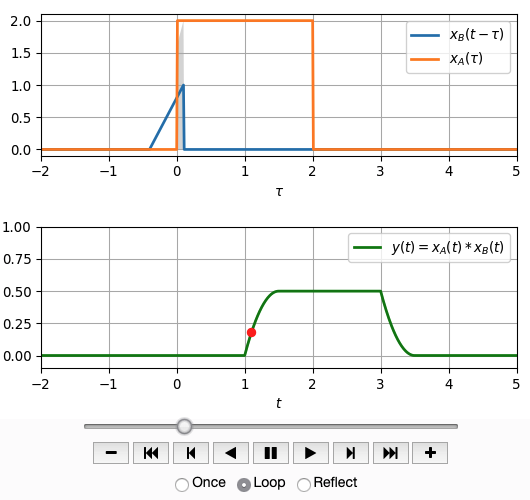
\includegraphics[width=\textwidth]{../convolution_ct/conv_var1_1_1D3D68B312.png}
\caption{Teilüberlappung vorn, also $y_1(t)$.}
\label{fig:1D3D68B312_v1_1}
\end{subfigure}
\begin{subfigure}{0.45\textwidth}
\centering
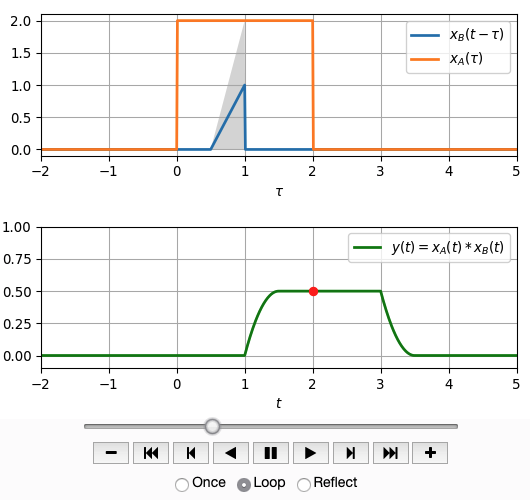
\includegraphics[width=\textwidth]{../convolution_ct/conv_var1_2_1D3D68B312.png}
\caption{Vollständige Überlappung, also $y_2(t)$.}
\label{fig:1D3D68B312_v1_2}
\end{subfigure}
\\
\begin{subfigure}{0.45\textwidth}
\centering
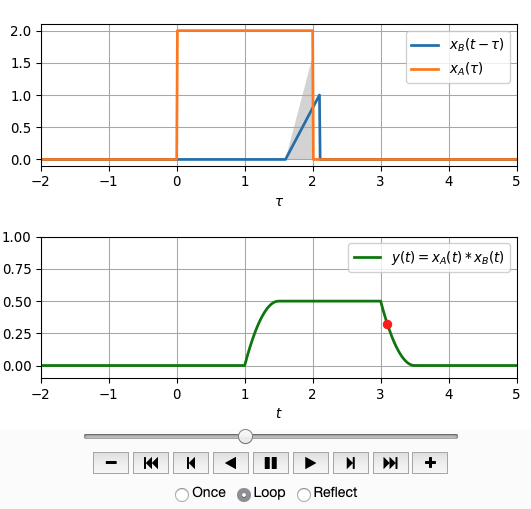
\includegraphics[width=\textwidth]{../convolution_ct/conv_var1_3_1D3D68B312.png}
\caption{Teilüberlappung hinten, also $y_3(t)$.}
\label{fig:1D3D68B312_v1_3}
\end{subfigure}
\begin{subfigure}{0.45\textwidth}
\centering
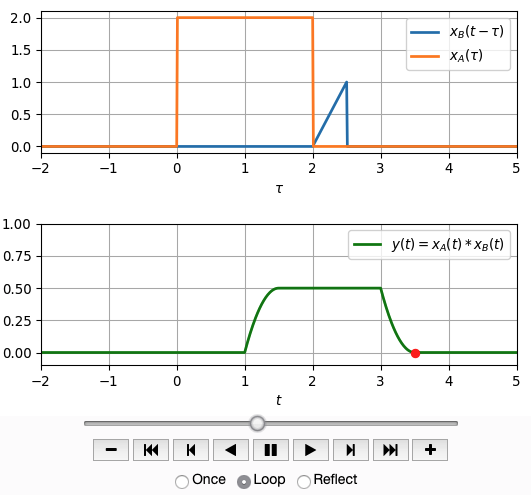
\includegraphics[width=\textwidth]{../convolution_ct/conv_var1_4_1D3D68B312.png}
\caption{Keine Überlappung hinten, also $y_4(t)$.}
\label{fig:1D3D68B312_v1_4}
\end{subfigure}
%
\caption{Faltungsprozess Variante I.
\texttt{convolution\_ct\_example1\_1D3D68B312.ipynb}}
\label{fig:1D3D68B312_v1}
\end{figure*}

\begin{ExCalc}
\textbf{Variante II: Zeitumkehr und Zeitverschiebung}  für $x(t)$
\begin{equation}
y(t) = \int\limits_{-\infty}^{+\infty} x(-\tau+t) h(\tau) \, \fsd \tau
\end{equation}
\begin{itemize}
  \item Schritt 1: Substitution $t\rightarrow \tau$ für $h(t)$
  \begin{equation}
  h(\tau) =
  \begin{cases}
  -2 \tau + 3 \quad \mathrm{für} \quad\red{1} \leq \tau \leq \red{\frac{3}{2}}\\
  0 \quad \mathrm{sonst}
  \end{cases}
  \end{equation}
  \item Schritt 2:  Substitution $t\rightarrow -\tau + t$ für $x(t)$
  \begin{equation}
  x(-\tau+t)=
  \begin{cases}
    2 \quad \mathrm{für} \quad 0 \leq -\tau+t \leq 2\\
    0 \quad \mathrm{sonst}
  \end{cases}
  \end{equation}
  \item Schritt 3:  Intervallgrenzen anpassen
  \begin{equation}
  x(-\tau+t)=
  \begin{cases}
    2 \quad \mathrm{für} \quad \blue{-2+t} \leq \tau \leq \blue{t}\\
    0 \quad \mathrm{sonst}
  \end{cases}
  \end{equation}
  \item Schritt 4: Stammfunktionansatz aufschreiben
  \begin{equation}
  y(t) =
  \int\limits_{a}^{b} x(-\tau+t) \cdot h(\tau) \fsd \tau =
  \int\limits_{a}^{b} 2 \cdot (-2 \tau + 3) \fsd \tau
  \end{equation}
  und berechnen zu
  \begin{equation}
  y(t) = -2 \tau^2 +6 \tau\bigg|_{\tau=a}^{\tau=b}
  \end{equation}
  Die \red{Intervall}\blue{grenzen} gehen als Integrationsbereiche $a,b$ in die Faltung ein.
  \item Schritt 5:  Signal-Überlappungen
  siehe Variante I
  % $x(t)$ ist endliches Signal von $t_1=0$ bis $t_2=2$
  %
  % $h(t)$ ist endliches Signal von $t_3=1$ bis $t_4=\frac{3}{2}$
  %
  % $y(t)$ wird daher ein endliches Signal von $t_1+t_3=1$ bis $t_2+t_4=\frac{7}{2}$ sein
  %
  % es gibt eine Teilüberlappung von $x(\tau)$ und $h(-\tau+t)$  'vorne' von
  % $t_1+t_3$ bis $t_1+t_3+T$
  %
  % es gibt eine Teilüberlappung von $x(\tau)$ und $h(-\tau+t)$  'hinten' von
  % $t_2+t_4-T$ bis $t_2+t_4$
  %
  % $T$ ist die Länge des kürzeren Signals, also hier $T=\frac{1}{2}$
  %
  % vollständige Überlappung hier für von $t = \frac{3}{2}$ bis $t=3$
  %
  % $y(t)=0$ für $t<(t_1+t_3)$ und $t\geq(t_2+t_4)$
  %
  % Diese Erkenntnisse in einer Formel
  % \begin{equation}
  % y(t) =
  % \begin{cases}
  %   y_1(t) \qquad \mathrm{für} \qquad 1 \leq t < \frac{3}{2}\\
  %   y_2(t) \qquad \mathrm{für} \qquad \frac{3}{2} \leq t < 3\\
  %   y_3(t) \qquad \mathrm{für} \qquad 3 \leq t < \frac{7}{2}\\
  %   y_4(t)=0 \qquad \mathrm{sonst}
  % \end{cases}
  % \end{equation}

  \item Schritt 6:  Stammfunktion mit Grenzen auswerten

  \begin{equation}
  y_1(t) = -2 \tau^2 +6 \tau\bigg|_{\tau=\red{1}}^{\tau=\blue{t}}
  = -2 t^2 + 6 t - 4
  \end{equation}

  \begin{equation}
  y_2(t) = -2 \tau^2 +6 \tau\bigg|_{\tau=\red{1}}^{\tau=\red{\frac{3}{2}}}  = \frac{1}{2}
  \end{equation}

  \begin{equation}
  y_3(t) = -2 \tau^2 +6 \tau\bigg|_{\tau=\blue{-2+t}}^{\tau=\red{\frac{3}{2}}} = +2 t^2 - 14 t + \frac{49}{2}
  \end{equation}

\end{itemize}
\end{ExCalc}

\begin{Loesung}
Das Ergebnis der Faltung, also das Ausgangssignal unseres LTI-Systems ist
wie erwartet gleich mit Variante I
\begin{align}
y(t) =
\begin{cases}
  y_1(t) = -2 t^2 + 6 t - 4 &\qquad \mathrm{für} \qquad 1 \leq t < \frac{3}{2}\\
  y_2(t) = \frac{1}{2}  &\qquad \mathrm{für} \qquad \frac{3}{2} \leq t < 3\\
  y_3(t) = +2 t^2 - 14 t + \frac{49}{2} &\qquad \mathrm{für} \qquad 3 \leq t < \frac{7}{2}\\
  y_4(t)=0 &\qquad \mathrm{sonst}
\end{cases}
\end{align}
Im Vergleich zu Variante I ist diese Lösung vielleicht
intuitiver, weil wir die Rechteckfunktion zeitlich verschieben und die
Integrallgrenzen schneller einleuchten.
%
Die Lösung wird in \fig{fig:1D3D68B312_v2} veranschaulicht für verschiedene
Zeiten $t$. In blau der zeitlich umgekehrte, verschobene Rechteckimpuls, in
orange die unverschobene Impulsantwort und in grün das Ausgangssignal der Faltung.
%
Wir sollten uns die \textbf{Unterschiede der Stammfunktionen und der Grenzen in den
Varianten I und II} genau anschauen.
Die Grenzen müssen stimmig sein zu der Funktion die verschoben wird.
%

Einem Rechteckimpuls sieht man nicht durch reines Hinschauen an, dass er
zeitlich gedreht wurde, hier ist also besondere Obacht erforderlich.
%
Gut gemeintes einfaches Integrieren erkaufen wir uns hier also mit tendenzieller
Verwirrung beim Signalspiegeln.
%
Erfahrungsgemäß braucht diese Rechnerei mal einen sehr ruhigen Moment und vertieftes
Sinnieren, während die Faltungsanimation in Dauerschleife läuft, irgendwann
wird klar, was wie verschoben werden muss und mit den Integrationsgrenzen verlinkt
ist.
%
\end{Loesung}















\begin{figure*}[h!]
\centering
\begin{subfigure}{0.45\textwidth}
\centering
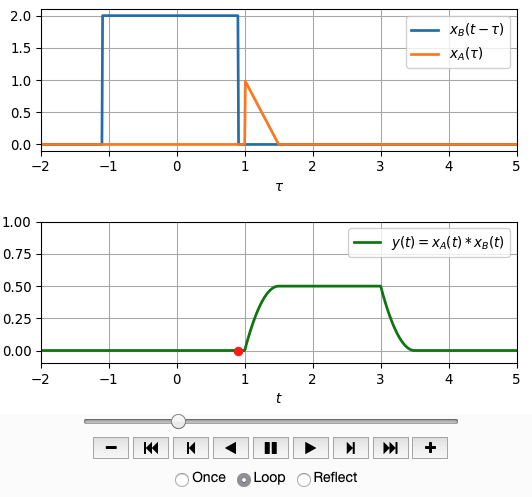
\includegraphics[width=\textwidth]{../convolution_ct/conv_var2_4_1D3D68B312.png}
\caption{Keine Überlappung vorne, also $y_4(t)$.}
\label{fig:1D3D68B312_v2_4}
\end{subfigure}
\begin{subfigure}{0.45\textwidth}
\centering
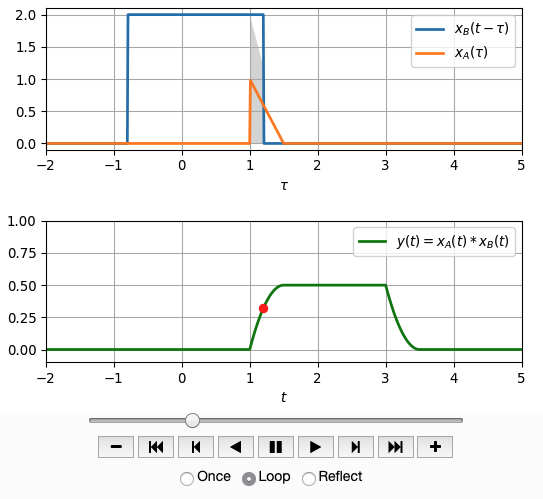
\includegraphics[width=\textwidth]{../convolution_ct/conv_var2_1_1D3D68B312.png}
\caption{Teilüberlappung vorn, also $y_1(t)$.}
\label{fig:1D3D68B312_v2_1}
\end{subfigure}
\\
\begin{subfigure}{0.45\textwidth}
\centering
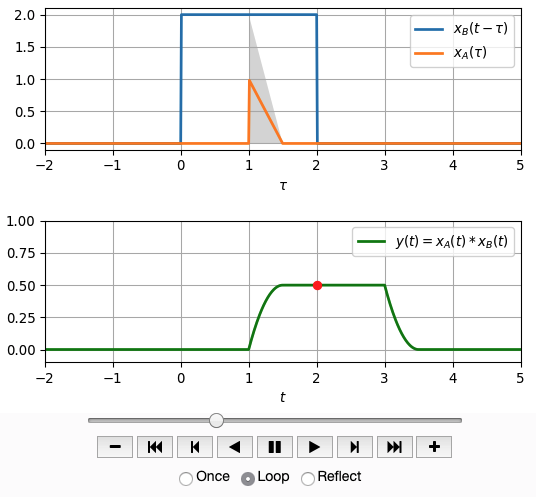
\includegraphics[width=\textwidth]{../convolution_ct/conv_var2_2_1D3D68B312.png}
\caption{Vollständige Überlappung, also $y_2(t)$.}
\label{fig:1D3D68B312_v2_2}
\end{subfigure}
\begin{subfigure}{0.45\textwidth}
\centering
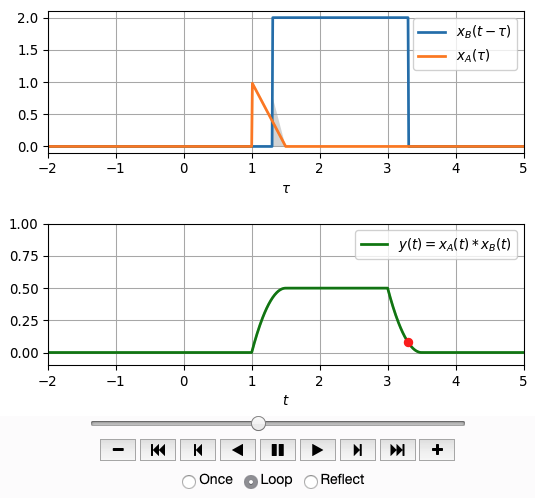
\includegraphics[width=\textwidth]{../convolution_ct/conv_var2_3_1D3D68B312.png}
\caption{Teilüberlappung hinten, also $y_3(t)$.}
\label{fig:1D3D68B312_v2_3}
\end{subfigure}
%
\caption{Faltungsprozess Variante II.
\texttt{convolution\_ct\_example1\_1D3D68B312.ipynb}}
\label{fig:1D3D68B312_v2}
\end{figure*}


\clearpage
\subsection{Faltung Rechteckimpuls mit Exponentialimpuls}
\label{sec:AF3B15E0D3}
\begin{Ziel}
Diese Aufgabe ist sehr ähnlich zu Aufgabe \ref{sec:1D3D68B312}.
Nur die Funktion von $h(t)$ ist verändert, alle Grenzen und
Längenbetrachtungen bleiben jedoch gleich. Das hat einen didaktischen
Hintergrund: Wir wollen hier zu der Erkenntnis kommen, dass eine exp()-Funktion
das Faltungsergebnis an den Sprungstellen anders 'glättet' als der Dreiecksimpuls
vorher.
Wenn wir $h(t)$ wieder als Impulsantwort eines LTI-System auffassen wollen,
heisst das, dass dieses System im Wesen ähnliche Dinge macht, aber im Detail
leicht anderes System-Verhalten hat.
\end{Ziel}
\textbf{Aufgabe} {\tiny AF3B15E0D3}: Berechnen Sie für die in der Skizze dargestellten
endlichen Signale $h(t)$ und $x(t)$ die Faltung $y(t)=x(t) \ast h(t)$.

\begin{tikzpicture}
\begin{axis}[
width=0.5\textwidth,
height=0.3\textwidth,
domain=1:3/2,
samples=20,
legend pos=outer north east,
xlabel = {t / s},
ylabel = {h(t), x(t)},
xmin=-1, xmax=4,
ymin=-0.1, ymax=2.1,
xtick={0,1,1.5,2},
ytick={0,1,2},
ymajorgrids=true,
xmajorgrids=true
]
\addplot[mark=None, color=C1, ultra thick] {exp(-6*(x-1))};
\addplot[mark=None, color=C0, ultra thick]
coordinates {(-1,0)(0,0)(0,2)(2,2)(2,0)(4,0)};
\addplot[mark=None, color=C1, ultra thick]
coordinates {(-1,0)(1,0)(1,1)};
\addplot[mark=None, color=C1, ultra thick]
coordinates {(1.5,0.05)(1.5,0)(4,0)};
\legend{$h(t)=\exp(-[t-1] \cdot 6) \cdot \mathrm{rect}([t-\frac{5}{4}] \cdot 2)$,
$x(t)=2\,\mathrm{rect}([t-1]\cdot \frac{1}{2})$}
\end{axis}
\end{tikzpicture}



\begin{Werkzeug}
Es ist mutmaßlich schöner zu integrieren, wenn wir $x(t)$ zeitlich umkehren und
verschieben, daher
\begin{equation}
y(t) = \int\limits_{-\infty}^{+\infty} x(-\tau+t) h(\tau) \, \fsd \tau
\end{equation}
also analog zur wahrscheinlich zugänglicheren Variante II aus Aufgabe
\ref{sec:1D3D68B312}.
\end{Werkzeug}


\begin{Ansatz}
Signale so darstellen, das wir den stückweisen Verlauf in seinen Grenzen angeben können.
Also: die Exponentialfunktion zeitlich verzögert um 1, schneller abfallend heißt zeitlich
gestaucht, Faktor 6
\begin{equation}
h(t) =
\begin{cases}
\e^{-[t-1]\cdot 6} \quad \mathrm{für} \quad 1 \leq t \leq \frac{3}{2}\\
0 \quad \mathrm{sonst}
\end{cases}
\end{equation}
Und der schon bekannte Rechteckimpuls
\begin{equation}
x(t)=
\begin{cases}
  2 \quad \mathrm{für} \quad 0 \leq t \leq 2\\
  0 \quad \mathrm{sonst}
\end{cases}
\end{equation}
Fassen wir $h(t)$ wieder als Impulsantwort eines LTI-Systems und $x(t)$ als
Eingangssignal in dieses auf. Wir werden gleich sehen, dass wir mit der Denke
sehr nah an der Praxis sind.
\end{Ansatz}




\begin{ExCalc}
Wir benutzen
\textbf{Variante II: Zeitumkehr und Zeitverschiebung}  für $x(t)$
\begin{equation}
y(t) = \int\limits_{-\infty}^{+\infty} x(-\tau+t) h(\tau) \, \fsd \tau
\end{equation}
und folgen unserem Algorithmus:
\begin{itemize}
  \item Schritt 1: Substitution $t\rightarrow \tau$ für $h(t)$
  \begin{equation}
  h(\tau) =
  \begin{cases}
  \e^{-[\tau-1]\cdot 6} \quad \mathrm{für} \quad\red{1} \leq \tau \leq \red{\frac{3}{2}}\\
  0 \quad \mathrm{sonst}
  \end{cases}
  \end{equation}
  \item Schritt 2:  Substitution $t\rightarrow -\tau + t$ für $x(t)$
  \begin{equation}
  x(-\tau+t)=
  \begin{cases}
    2 \quad \mathrm{für} \quad 0 \leq -\tau+t \leq 2\\
    0 \quad \mathrm{sonst}
  \end{cases}
  \end{equation}
  \item Schritt 3:  Intervallgrenzen anpassen
  \begin{equation}
  x(-\tau+t)=
  \begin{cases}
    2 \quad \mathrm{für} \quad \blue{-2+t} \leq \tau \leq \blue{t}\\
    0 \quad \mathrm{sonst}
  \end{cases}
  \end{equation}
  \item Schritt 4: Stammfunktionansatz
  \begin{equation}
  y(t) =
  \int\limits_{a}^{b} x(-\tau+t) \cdot h(\tau) \fsd \tau =
  \int\limits_{a}^{b} 2 \cdot (\e^{-[\tau-1]\cdot 6}) \fsd \tau
  \end{equation}
  und berechnen zu (auch noch ein eher triviales Integral)
  \begin{equation}
  y(t) = -\frac{1}{3}\e^{-[\tau-1]\cdot 6}\bigg|_{\tau=a}^{\tau=b}
  \end{equation}
  Die \red{Intervall}\blue{grenzen} gehen als Integrationsbereiche $a,b$ in die Faltung ein.

  \item Schritt 5:  Signal-Überlappungen

  $x(t)$ ist endliches Signal von $t_1=0$ bis $t_2=2$

  $h(t)$ ist endliches Signal von $t_3=1$ bis $t_4=\frac{3}{2}$

  $y(t)$ wird daher ein endliches Signal von $t_1+t_3=1$ bis $t_2+t_4=\frac{7}{2}$ sein

  es gibt eine Teilüberlappung von $x(\tau)$ und $h(-\tau+t)$  'vorne' von
  $t_1+t_3$ bis $t_1+t_3+T$

  es gibt eine Teilüberlappung von $x(\tau)$ und $h(-\tau+t)$  'hinten' von
  $t_2+t_4-T$ bis $t_2+t_4$

  $T$ ist die Länge des kürzeren Signals, also hier $T=\frac{1}{2}$

  vollständige Überlappung hier für von $t = \frac{3}{2}$ bis $t=3$

  $y(t)=0$ für $t<(t_1+t_3)$ und $t\geq(t_2+t_4)$

  Diese Erkenntnisse in einer Formel
  \begin{equation}
  y(t) =
  \begin{cases}
    y_1(t) \qquad \mathrm{für} \qquad 1 \leq t < \frac{3}{2}\\
    y_2(t) \qquad \mathrm{für} \qquad \frac{3}{2} \leq t < 3\\
    y_3(t) \qquad \mathrm{für} \qquad 3 \leq t < \frac{7}{2}\\
    y_4(t)=0 \qquad \mathrm{sonst}
  \end{cases}
  \end{equation}

  \item Schritt 6:  Stammfunktion mit Grenzen auswerten

  \begin{equation}
  y_1(t) = -\frac{1}{3}\e^{-[\tau-1]\cdot 6}\bigg|_{\tau=\red{1}}^{\tau=\blue{t}}
  = \frac{1}{3}\left(1-\e^{-[t-1] \cdot 6}\right)
  \end{equation}

  \begin{equation}
  y_2(t) = -\frac{1}{3}\e^{-[\tau-1]\cdot 6}\bigg|_{\tau=\red{1}}^{\tau=\red{\frac{3}{2}}}  =
  \frac{1}{3}\left(1-\e^{-3}\right) \approx 0.316737...
  \end{equation}

  \begin{equation}
  y_3(t) = -\frac{1}{3}\e^{-[\tau-1]\cdot 6}\bigg|_{\tau=\blue{-2+t}}^{\tau=\red{\frac{3}{2}}} =
  \frac{1}{3}\left(\e^{-[t-3] \cdot 6} - \e^{-3}\right)
  \end{equation}
\end{itemize}
\end{ExCalc}


\begin{Loesung}
Das gesuchte Faltungsergebnis ist also
\begin{align}
y(t) =
\begin{cases}
  y_1(t) = \frac{1}{3}\left(1-\e^{-[t-1] \cdot 6}\right) &\qquad \mathrm{für} \qquad 1 \leq t < \frac{3}{2}\\
  y_2(t) = \frac{1}{3}\left(1-\e^{-3}\right) \approx 0.316737 &\qquad \mathrm{für} \qquad \frac{3}{2} \leq t < 3\\
  y_3(t) = \frac{1}{3}\left(\e^{-[t-3] \cdot 6} - \e^{-3}\right) &\qquad \mathrm{für} \qquad 3 \leq t < \frac{7}{2}\\
  y_4(t)=0 &\qquad \mathrm{sonst}
\end{cases}
\end{align}

In \fig{fig:AF3B15E0D3_v2} ist der Faltungsprozess veranschaulicht.
%
Stellen wir im Vergleich zu Aufgabe \ref{sec:1D3D68B312} fest, dass
%
\begin{itemize}
  \item die Grenzen für Signalabschnitte gleich geblieben sind (diese Aufgabe war ja so
  ausgelegt)
  \item $y_2(t)$ wieder ein konstanten Verlauf hat, nur diesmal mit der Amplitude von ca.
  $0.316737$. Die Fläche des Exponentialimpulses ist ja kleiner als die des Dreickimpulses
  aus Aufgabe \ref{sec:1D3D68B312}
  \item die Gleichungen, welche die stückweisen Abschnitte definieren diesmal mit der
  Exponentialfunktion beschrieben werden. Auch das sollte wieder einleuchten,
  beim Integrieren einer Exponentialfunktion resultiert wieder eine Exponentialfunktion
\end{itemize}
%
\textbf{Ladekurven Kondensator?!?} Wenn wir uns das Faltungsergebnis $y(t)$
(grüner Graph) und die Ergebnisgleichungen anschauen, wird uns
vielleicht eine verblüffende Ähnlichkeit zu Auf-/Entladekurven eines
RC-Gliedes auffallen. Wir schauen uns das in der nächsten Aufgabe \ref{sec:C964DD7400}
genauer an. Hier schon mal soviel, es ist sehr ähnlich aber nicht exakt identisch.
Der Grund liegt in der hier betrachteten \textbf{endlichen} Impulsantwort. Ein
RC-Glied hat eine \textbf{unendliche} Impulsantwort.
\end{Loesung}


\begin{figure*}[h!]
\centering
\begin{subfigure}{0.45\textwidth}
\centering
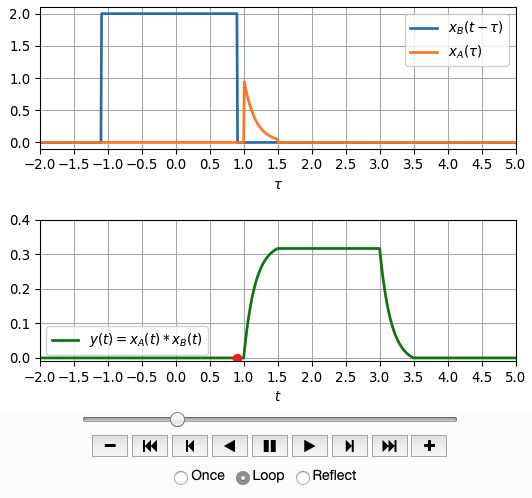
\includegraphics[width=\textwidth]{../convolution_ct/conv_var2_4_AF3B15E0D3.png}
\caption{Keine Überlappung vorne, also $y_4(t)$.}
\label{fig:AF3B15E0D3_v2_4}
\end{subfigure}
\begin{subfigure}{0.45\textwidth}
\centering
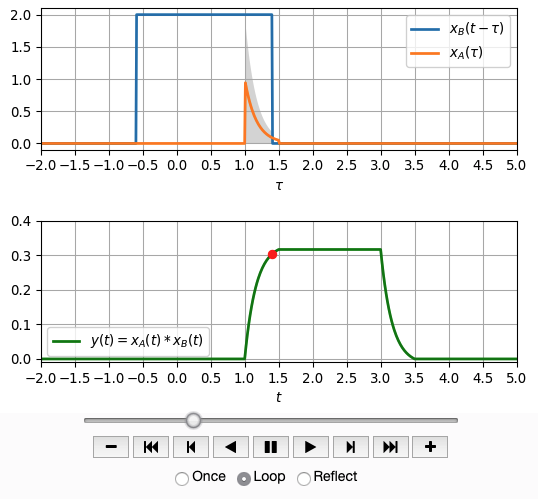
\includegraphics[width=\textwidth]{../convolution_ct/conv_var2_1_AF3B15E0D3.png}
\caption{Teilüberlappung vorn, also $y_1(t)$.}
\label{fig:AF3B15E0D3_v2_1}
\end{subfigure}
\\
\begin{subfigure}{0.45\textwidth}
\centering
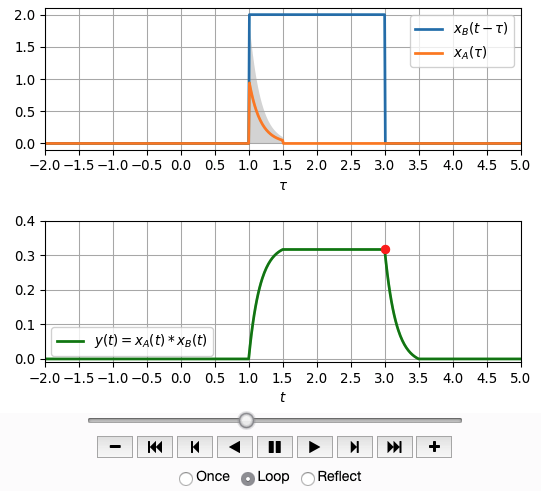
\includegraphics[width=\textwidth]{../convolution_ct/conv_var2_2_AF3B15E0D3.png}
\caption{Vollständige Überlappung, also $y_2(t)$.}
\label{fig:AF3B15E0D3_v2_2}
\end{subfigure}
\begin{subfigure}{0.45\textwidth}
\centering
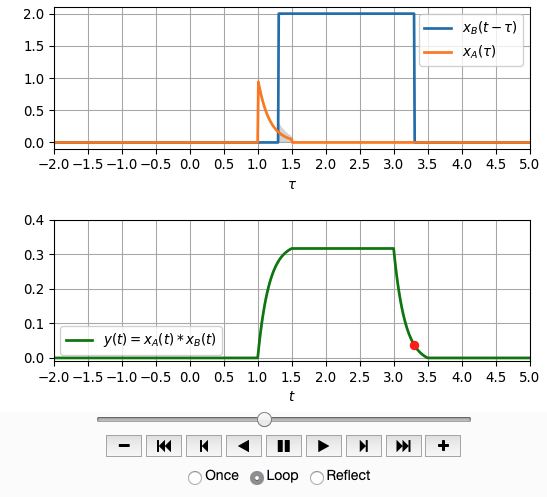
\includegraphics[width=\textwidth]{../convolution_ct/conv_var2_3_AF3B15E0D3.png}
\caption{Teilüberlappung hinten, also $y_3(t)$.}
\label{fig:AF3B15E0D3_v2_3}
\end{subfigure}
%
\caption{Faltungsprozess Aufgabe \ref{sec:AF3B15E0D3}.
\texttt{convolution\_ct\_example2\_AF3B15E0D3.ipynb}}
\label{fig:AF3B15E0D3_v2}
\end{figure*}



\clearpage
\subsection{Faltung Rechteckimpuls mit Exponentialfunktion}
\label{sec:C964DD7400}
\begin{Ziel}
Wir werden anhand einer speziellen Faltung eines endlichen Signals mit
einem unendlichen Signal, einen ganz fundamentalen Link zur Elektrotechnik
und DGLs 1. Ordnung mit konstanten Koeffizienten herstellen:
Sprungartige Spannungsänderungen an passiven Energiespeichern (Auf-/Entladen) können wir
sehr elegant mit Signal-und Systemtheorie Werkzeugen berechnen. Es wird mit
der Laplace Transformation später sogar noch eleganter.
\end{Ziel}
\textbf{Aufgabe} {\tiny C964DD7400}: Für das unten abgebildete RC-Glied
(Annahme: ideale Bauelemente)
gilt die \textbf{Impulsantwort} (wir nehmen LTI System-Eigenschaften an)
\begin{equation}
h(t) = \frac{1}{T_\mathrm{RC}} \cdot \e^{-\frac{t}{T_\mathrm{RC}}}
\qquad \mathrm{für} \qquad t \geq 0
\qquad \mathrm{mit} \qquad T_\mathrm{RC} = R \cdot C
\end{equation}
Wir betrachten das RC-Glied als ruhend, also $y(0)=0$.
%
Berechnen Sie für $T_\mathrm{RC}=\frac{1}{5}$ s und für das unten dargestellte
Eingangssignal $x(t)$ das Faltungsergebnis $y(t)=x(t) \ast h(t)$.
%
\begin{center}
\begin{circuitikz}[european, scale=0.75]
\node (in) at (1,0){};
\node (in_ground) at (1,-3){};
\node (out) at (4,0){};
\node (out_ground) at (4,-3){};
\draw (in) to [R,l_=$R$,o-] (3,0);
\draw (3,0) to [short,-o,] (out);
\draw (3,0) to [C,l_=$C$,*-*] (3,-3);
\draw (in_ground) to [short,o-o] (out_ground);
\path[draw, bend right, ->, >=latex] (in) edge node[left]{Eingangsspannung $x(t)$} (in_ground);
\path[draw, bend left, ->, >=latex] (out) edge node[right]{Ausgangsspannung $y(t)$} (out_ground);
\end{circuitikz}
\end{center}
%
\begin{tikzpicture}
\begin{axis}[
width=0.5\textwidth,
height=0.3\textwidth,
domain=0:4,
samples=50,
legend pos=outer north east,
xlabel = {t / s},
ylabel = {h(t), x(t)},
xmin=-1, xmax=4,
ymin=-0.1, ymax=1.1,
xtick={0,1,2,3},
ytick={0,0.5,1,1.5,2},
ymajorgrids=true,
xmajorgrids=true
]
\addplot[mark=None, color=C0, ultra thick]
coordinates {(-1,0)(0,0)(0,1)(2,1)(2,0)(4,0)};
\addplot[mark=None, color=C1, ultra thick]
coordinates {(-1,0)(0,0)(0,1)};
\addplot[mark=None, color=C1, ultra thick] {exp(-5*(x))};
\legend{$x(t)=\mathrm{rect}([t-1]\cdot \frac{1}{2})$,
$\frac{1}{5} \cdot h(t)=\exp(- t \cdot 5) \cdot \epsilon(t)$}
\end{axis}
\end{tikzpicture}

\noindent\textbf{Hinweis 1}: Wir werden nach der Übung~\ref{sec:ue3_laplace} (3) in der Lage sein, $h(t)$ elegant herzuleiten.
Nehmen wir das an dieser Stelle mal hin, aber bemerken auch, dass wir
diese Art Formel beim Kondensator eh schon mal gesehen haben, mutmaßlich aber
nicht im Kontext einer Impulsantwort.

\noindent\textbf{Hinweis 2}: In der Elektrotechnik verwenden wir gerne $\tau$ für die Zeitkonstante. Weil das
aber unsere Hilfsvariable in der Faltung ist, geben wir der Zeitkonstante des RC-Glieds die Variable
$T_\mathrm{RC}$.

\noindent\textbf{Hinweis 3}: Aufgabe \ref{sec:AF3B15E0D3} behandelte den \textbf{endlichen Exponentialimpuls}
mit einer Zeitkonstante $1/6$ s, hier verwenden wir die abfallende Exponentialfunktion
die sich nur asymptotisch gegen Null nähert, die also eine \textbf{unendliche Impulsantwort}
darstellt. Der schöneren Anschauung wegen, wählen wir $T_\mathrm{RC}=1/5$ s, weil
dann bei 1 s zu 99\% der finale Lade-/Entlade-Amplitudenwert erreicht ist
(vgl. $5 T_\mathrm{RC}$-Regel).

\noindent\textbf{Hinweis 4}: Machen wir uns noch klar, dass wir es hier mit der DGL 1. Ordnung
mit konstanten Koeffizienten
\begin{equation}
T_\mathrm{RC} \frac{\fsd y(t)}{\fsd t} + y(t) = x(t)
\end{equation}
mit $y(0)=0$ zu tun haben und überlegen, wie wir die Aufgabe mit
typischem Mathe-DGL Handwerk lösen würden. Siehe auch SigSys-Klausur WS19/20 Aufgabe 1.

\begin{Werkzeug}
Es ist mutmaßlich wieder schöner zu integrieren,
wenn wir $x(t)$ zeitlich umkehren und verschieben, daher Faltungsintegral
\begin{equation}
y(t) = \int\limits_{-\infty}^{+\infty} x(-\tau+t) h(\tau) \, \fsd \tau
\end{equation}

\end{Werkzeug}
\begin{Ansatz}
Die Signale zum Falten sind
\begin{equation}
h(t) =
\begin{cases}
\frac{1}{\frac{1}{5}} \e^{-\frac{t}{\frac{1}{5}}} = 5 \e^{-5 t} \quad \mathrm{für} t \geq 0\\
0 \quad \mathrm{sonst}
\end{cases}
\end{equation}
\begin{equation}
x(t)=
\begin{cases}
  1 \quad \mathrm{für} \quad 0 \leq t \leq 2\\
  0 \quad \mathrm{sonst}
\end{cases}
\end{equation}
\end{Ansatz}

\begin{ExCalc}
Wir benutzen
\textbf{Variante II: Zeitumkehr und Zeitverschiebung}  für $x(t)$
\begin{equation}
y(t) = \int\limits_{-\infty}^{+\infty} x(-\tau+t) h(\tau) \, \fsd \tau
\end{equation}
Wir können diesmal nicht unseren bereits etablierten Algorithmus verwenden, weil
der nur funktioniert, wenn beide Signale endliche Länge haben.
%
Machen wir uns hier stattdessen zu nutze, dass die Rechteckfunktion durch zwei
Sprungfunktionen dargestellt werden kann, nämlich $x(t) = \epsilon(t) - \epsilon(t-2)$.
%
Es gilt das Superpositionsprinzip bei LTI-Systemen. Daher
können wir für die beiden einzelnen Sprünge die Faltungen einzeln ausrechnen.
%
Das gelingt besonders elegant, wenn man für die Faltung die Sprünge als die
zeitumgekehrten und verschobenen Signale auffasst (damit wäre Klausuraufgabe 1
vom SS2019 ganz schnell berechnet).
%
Konkret also: Faltung mit der Sprungfunktion $x_1(t) = \epsilon(t)$ führt auf
\begin{equation}
y_1(t) = \int\limits_{0}^{t} 1 \cdot 5 \e^{- 5 \tau} \fsd \tau= \left(1-\e^{-5 t}\right)
\qquad \mathrm{für} \qquad t \geq 0
\end{equation}
%
Faltung mit der Sprungfunktion $x_2(t) = -\epsilon(t-2)$ führt auf
\begin{equation}
y_2(t) =
\begin{cases}
  0 &\qquad \mathrm{für} \qquad t < 2\\
  \int\limits_{2}^{t} -1 \cdot 5 \e^{- 5 [\tau-2]}  \fsd \tau = \left( \e^{-5 [t-2]}-1\right) &\qquad \mathrm{für} \qquad t \geq 2
\end{cases}
\end{equation}
%
% Bitte nochmal mit Wolfram Alpha gegenchecken:
% Ansatz für gedrehte Impulsantwort
% integrate -step(tau-2)*5*exp(5*tau-5*t) d tau from 0 to t
% oder Ansatz für gedrehten Reckteckimpuls
% integrate -step(-tau+t-2)*5*exp(-5*tau) d tau from 0 to t

% Mit dem zweiteren, hab ich dann für 2.217 die beiden Funktionen verschoben (bzgl. tau) und die Integralgrenzen angepasst
% integrate -step(-tau+t)*5*exp(-5*(tau-2)) d tau from 2 to t
% und wenn wir dann explizit erwähnen, dass y(t) nur für t>=2, brauchen wir die step funktion im Integral nicht mehr und wir können mit dem Integral
% integrate -5*exp(-5*(tau-2)) d tau from 2 to t
% rechnen.
% %
% Es gilt das Superpositionsprinzip bei LTI-Systemen, also einer Eingangssumme
% $x(t) = x_1(t) + x_2(t) = \epsilon(t) - \epsilon(t-2)$
% folgt die Ausgangssumme $y(t) = y_1(t) + y_2(t)$.
\end{ExCalc}

\begin{Loesung}
Das Endergebnis lautet mit Superposition
\begin{equation}
y(t) = y_1(t) + y_2(t) =
  \begin{cases}
  \left(1-\e^{-5 t}\right) &\qquad \mathrm{für} \qquad 0 \leq t < 2\\
  \left(1-\e^{-5 t}\right) + \left( \e^{-5 [t-2]}-1\right) = \e^{-5 [t-2]} - \e^{-5 t}
  &\qquad \mathrm{für} \qquad t \geq 2
  \end{cases}
\end{equation}
und wir erkennen im ersten Teil der Gleichung die typische Aufladekurve des
Kondensators. Im zweiten Teil ist die nicht ganz so offensichtliche Entladekurve
zu sehen, wir entladen erst zum Zeitpunkt $t=2$ s, das muss in der exp()-Funktion
als Zeitverschiebung mit berücksichtigt werden.
%
Die gewählte Zeitkonstante ist sehr kurz im Vergleich zum Rechtecklänge, daher
kann man für den Kondensator mit guter Näherung drei Zustände während des
Anlegens von $x(t)$ definieren:
\begin{itemize}
  \item für $0<t<1$ Aufladen
  \item für $1<t<2$ Geladen
  \item für $2<t<3$ Entladen
\end{itemize}
Wie oben schon erwähnt, erfolgt vollständiges Aufladen und Entladen mit asymptotischer
Annäherung an den Endzustand.

Spannende Frage zum Sinnieren oder vielleicht sogar Rechnen:
Wie schaut das Ausgangssignal $y(t)$ aus, wenn man den Rechtecksprung sehr,
sehr, sehr kurz macht und vielleicht sogar Fläche 1 sicherstellt?

Spannender Link I: Wir haben mit
\begin{align}
y_1(t) =
\begin{cases}
1-\e^{-5 t} \quad \text{für} \quad t\geq 0\\
0 \quad \text{sonst}
\end{cases}
\end{align}
die sogenannte \textbf{Sprungantwort} $h_\epsilon(t)$ des Systems berechnet,
sozusagen als Abfallprodukt, weil wir die Sprungfunktion als Systemeingang gewählt
haben, und das System eben antwortet mit der ... Sprungantwort.

Spannender Link II: Die \textbf{Impulsantwort} $h(t)$ ist direkt proportional zur
Entladekurve eines Kondensators, wenn der Kondensator zum Zeitpunkt $t=0$
vollständig auf $U_q$ aufgeladen war und ab $t=0+$ die Entladung erfolgt.
Aus der Elektrotechnik wissen wir, dass dann $y(t) = U_q \e^{-\tau/T_\mathrm{RC}}$ gilt,
wir sehen Ähnlichkeiten mit $h(t) = \frac{1}{T_\mathrm{RC}} \cdot \e^{-\frac{t}{T_\mathrm{RC}}}$...

Wir bekommen langsam ein Gespür für die größeren Zusammenhänge und
warum SigSys nützlich sein könnte.
\end{Loesung}


\begin{figure*}[h!]
\centering
\begin{subfigure}{0.45\textwidth}
\centering
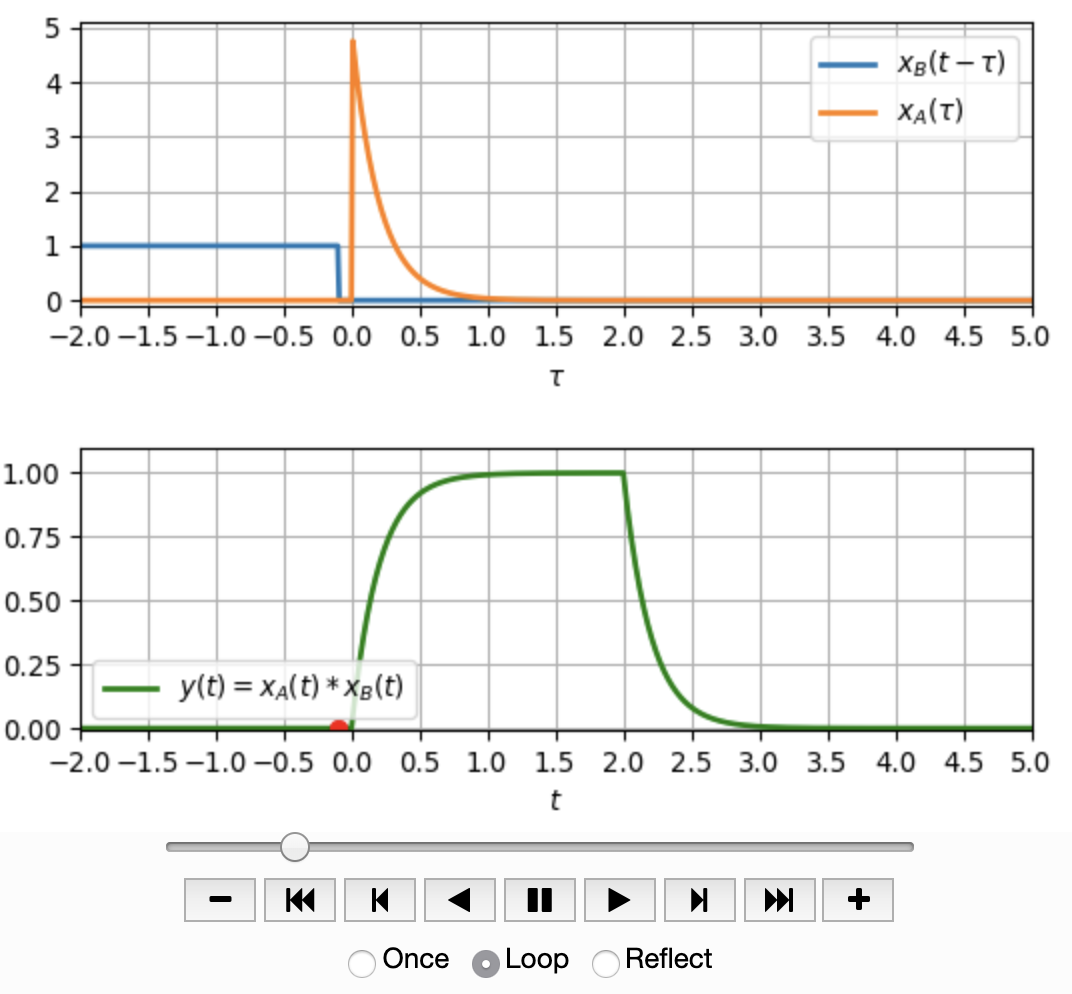
\includegraphics[width=\textwidth]{../convolution_ct/conv_var2_1_C964DD7400.png}
\caption{Keine Überlappung vorne.}
\label{fig:C964DD7400_v2_1}
\end{subfigure}
\begin{subfigure}{0.45\textwidth}
\centering
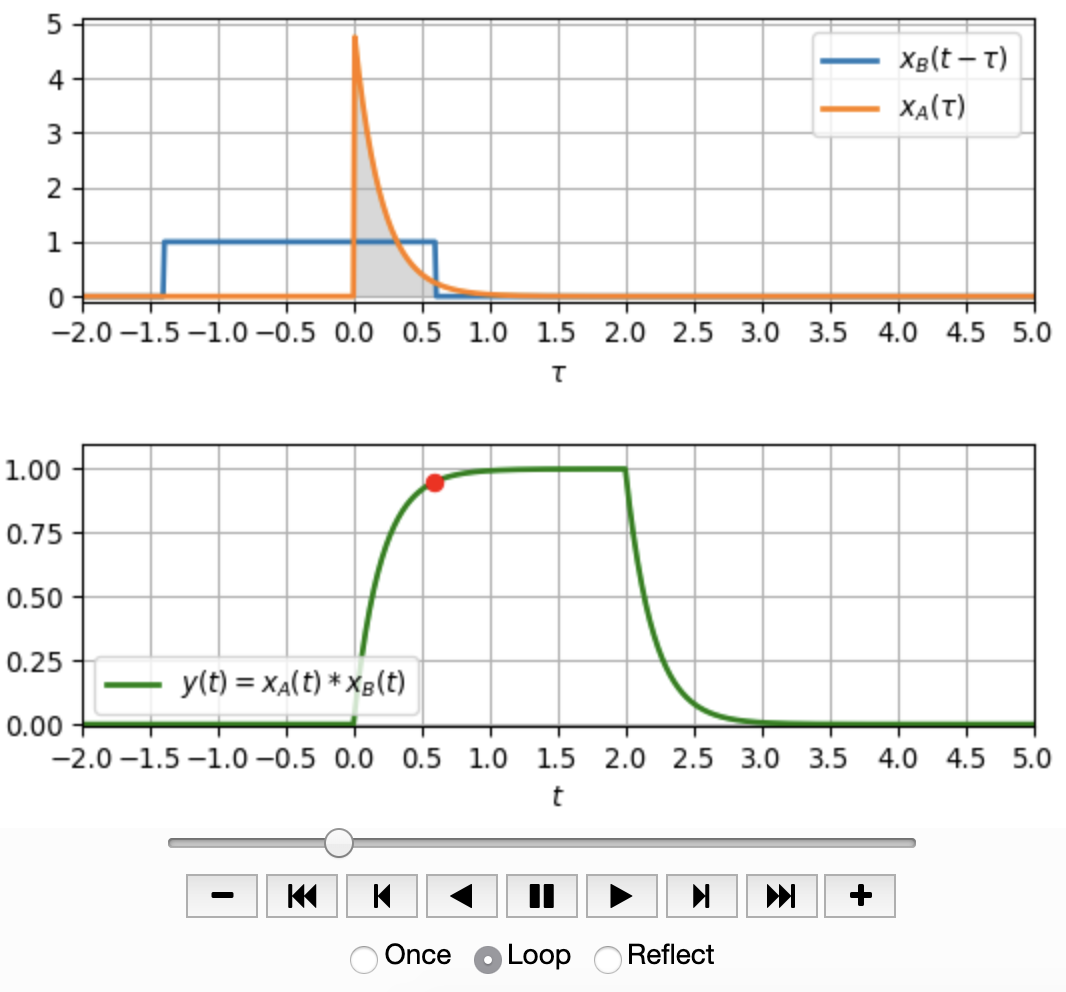
\includegraphics[width=\textwidth]{../convolution_ct/conv_var2_2_C964DD7400.png}
\caption{Teilüberlappung, Ladezustand: 95\%.}
\label{fig:C964DD7400_v2_2}
\end{subfigure}
\\
\begin{subfigure}{0.45\textwidth}
\centering
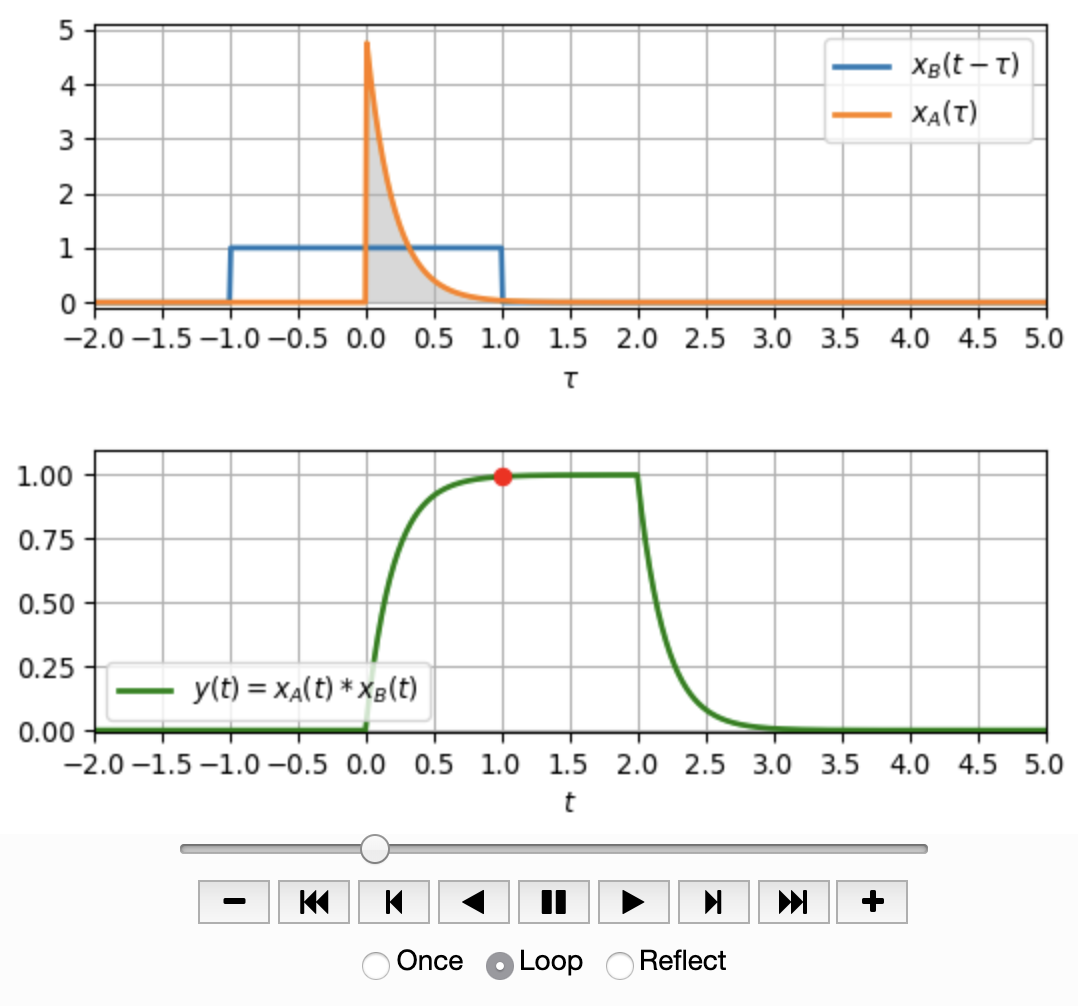
\includegraphics[width=\textwidth]{../convolution_ct/conv_var2_3_C964DD7400.png}
\caption{Teilüberlappung, Ladezustand: 99\%.}
\label{fig:C964DD7400_v2_3}
\end{subfigure}
\begin{subfigure}{0.45\textwidth}
\centering
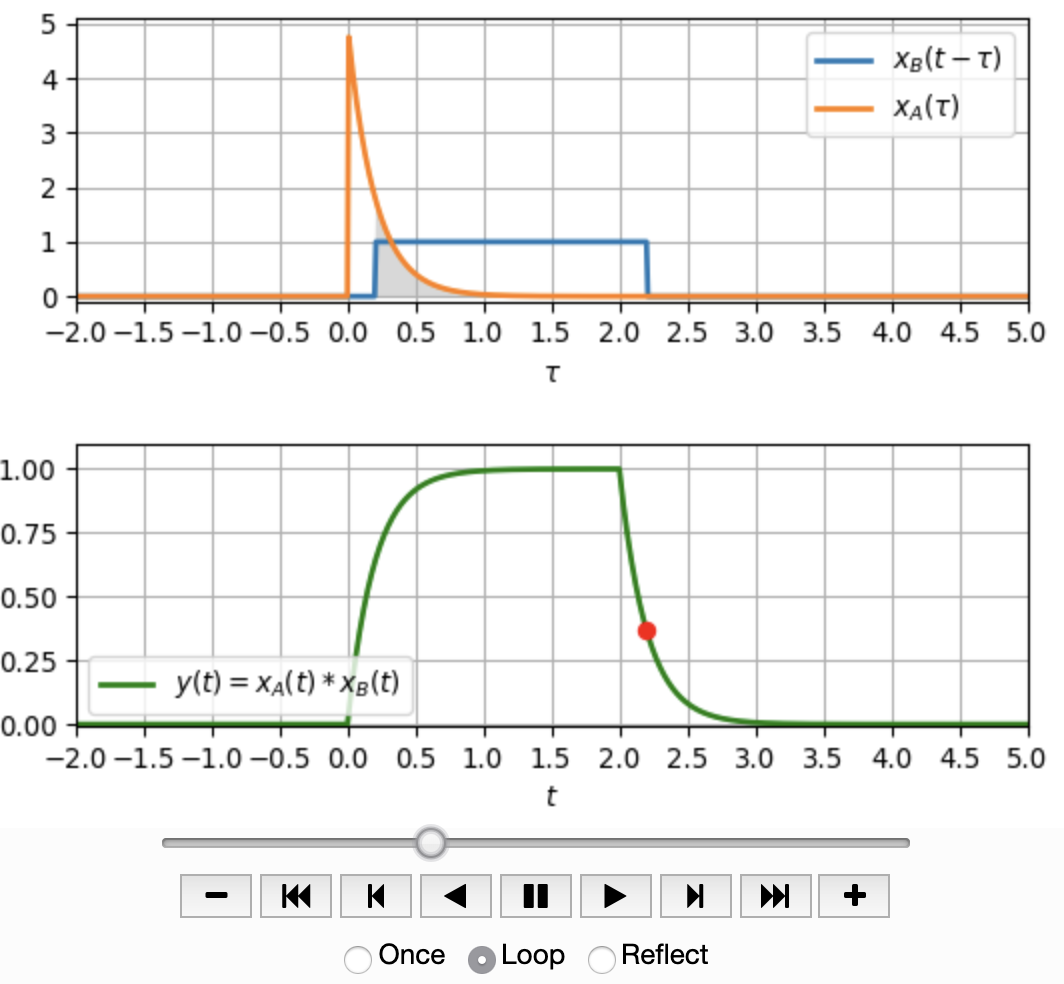
\includegraphics[width=\textwidth]{../convolution_ct/conv_var2_4_C964DD7400.png}
\caption{Teilüberlappung, Ladezustand: 37\% .}
\label{fig:C964DD7400_v2_4}
\end{subfigure}
%
\caption{Faltungsprozess Aufgabe \ref{sec:C964DD7400}.
\texttt{convolution\_ct\_example3\_C964DD7400.ipynb}}
\label{fig:C964DD7400_v2}
\end{figure*}

\newpage
Wolfram Alpha löst einfache Faltungen analytisch und plotted die Signalverläufe
des Ergebnissignals. Folgende Beispiele mit immer
dem gleichen Rechtecksignal, aber unterschiedlichen Impulsantworten

\verb| Convolve[rect(1/4*(t-2)), 2*exp(-t/(1/2))*Step(t)]|

\verb| Convolve[rect(1/4*(t-2)), tri(t)*Step(t)]|

\verb| Convolve[rect(1/4*(t-2)), tri(t-1) * rect((t-1/2))]|

\verb| Convolve[rect(1/4*(t-2)), rect(t-1/2)]|

verdeutlichen nochmal schön die unterschiedlichen Auflade- und Entlade-Vorgänge
bedingt durch unterschiedliche Impulsantwortfunktionen. Wenn wir diese Verläufe
durch Überlegung schematisch herleiten können, haben wir im Grunde das Wesen der
Faltung verstanden.
  % UE 2, signal ops, LTI, conv

\setcounter{section}{2}
%%------------------------------------------------------------------------------
\clearpage
\section{UE 3: Laplace Transformation}
\label{sec:ue3_laplace}
%
Wir haben Laplace Transformation sicherlich schon in einer Mathe Vorlesung
kennengelernt.
Laplace Transformation ist eine Integraltransformation aus der Familie
\begin{equation}
F(y) = \int\limits_{x_1}^{x_2} f(x) \cdot K(x,y) \fsd x
\end{equation}
mit dem Integralkern $K(x,y) = \e^{-x\,y}$.
Wir verwenden in SigSys vorwiegend für die Variable $x$ die Zeit $t$ und für
$y$ die Laplace/Bild Variable $s\in\mathbb{C}$ (in älterer Literatur finden
wir auch oft die Variable $p$, wahrscheinlich um den Link zur Namensgebung
La\underline{p}lace zu machen).
Als Grenzen benutzen wir oft $x_1=0$ und $x_2=\infty$ um kausale Signale und
Systeme beschreiben zu können.
%
Die Rücktransformation ist wegen $s\in\mathbb{C}$ ein komplexes Wegintegral.

Wir verwenden Signal-Transformationen, in der Hoffnung, dass a) Probleme im
transformierten Signalraum, dem sogenannten Bildbereich einfacher zu lösen
sind als im Originalbereich und b) dass Signale einfacher/kompakter darstellbar
sind (vgl. periodisches Signal vs. Koeffizienten der Fourierreihe).
%
Die Wahl der geeignetsten Transformation ist dabei entscheidend, weil eine
ungeeignete das Problem auch komplizierter machen kann.
%
Die Laplace Transformation ist nun deswegen herausragend geeignet, weil
wir Signale \textbf{und} LTI-Systeme analysieren \textbf{und} synthetisieren
können und deswegen Signale mit Systemen elegant und konsistent verknüpfen können.

Wir sollten uns klarmachen, dass der \textbf{Wunsch nach einem einfacherem Operator
für die zeitliche Ableitung} ein Ausgangspunkt für die Erfindung der Laplace
Transformation ist; das sehr lesenswerte, zeitlose Lehrwerk \cite{LangeSigSys1} enthält
einen Abschnitt über die Entwicklungshistorie bis in die 1970er.
Statt Ableiten, also Multiplizieren
\begin{equation}
  \frac{\fsd }{\fsd t} (\cdot) \rightarrow s(\cdot ) \text{ mit } s \in \mathbb{C}
\end{equation}
unter Beibehaltung der Skalierungseigenschaft (Multiplikation mit Konstanten)
und Additionseigenschaft (Superposition).
%
Viele Mathematiker*innen haben sich an dieser Fragestellung der Operatorentheorie
abgearbeitet, sie ist ja zunächst aus rein mathematischer hochspannend, und
es hat sich herausgestellt, dass ein Spezialfall
(nämlich für $y=s\in\mathbb{C}$\footnote{die Integraltransformation mit $y=\im\omega$
, also $y$ rein imaginär, erfüllt unsere Anforderung an den neuen Operator nicht ganz,
weil eben der für bestimmte Betrachtungen wichtige Realteil in $y$ fehlt.
Wir werden sie aber trotzdem sehr nützlich finden
für SigSys, es ist die Fouriertransformation.})
der obigen
Integraltransformation genau das gewünschte leistet. Es wurde definiert
\begin{align}
\mathcal{L}\{x(t)\} = \int\limits_{t=0}^{\infty} x(t) \cdot \e^{-s\,t} \fsd t,
\end{align}
später deklariert als einseitige Laplace Transformation, benutzbar
für kausale Signale.
%
Die Laplace Transformation ist ein linearer Operator, d.h.
es gilt Additionseigenschaft
\begin{align}
\mathcal{L}\{x_1(t)+x_2(t)\} = \mathcal{L}\{x_1(t)\} + \mathcal{L}\{x_2(t)\}
\end{align}
und die Skalierungseigenschaft
\begin{align}
\mathcal{L}\{a x(t)\} = a \mathcal{L}\{x(t)\}.
\end{align}

Schauen wir uns kurz an, wie der Wunsch nach
$\frac{\fsd }{\fsd t} (\cdot) \rightarrow s(\cdot )$
mittels der Integraltransformation erfüllt wird, also was passiert mit
\begin{align}
\mathcal{L}\{\frac{\fsd }{\fsd t}  x(t)\} &= \int\limits_{t=0}^{\infty} \frac{\fsd }{\fsd t}  x(t) \cdot \e^{-s\,t} \fsd t
\end{align}
Die partielle Integration hilft dies anders darzustellen
\begin{align}
&\int u v' \fsd t + \int v u' \fsd t = u\,v\\
&\int u v' \fsd t = u\,v - \int v u' \fsd t\\
&u = \e^{-s\,t}\qquad u' = -s\,\e^{-s\,t}\\
&v = x(t)\qquad v' = \frac{\fsd }{\fsd t}  x(t)\\
&\int\limits_{t=0}^{\infty} \e^{-s\,t} \frac{\fsd }{\fsd t}  x(t) \, \fsd t
= \e^{-s\,t}\,x(t)\bigg|_{t=0}^{\infty} - \int\limits_{t=0}^{\infty} x(t) \cdot (-s\,\e^{-s\,t}) \, \fsd t\\
&\int\limits_{t=0}^{\infty} \e^{-s\,t} \frac{\fsd }{\fsd t}  x(t) \, \fsd t
= s \cdot \int\limits_{t=0}^{\infty} x(t) \e^{-s\,t} \, \fsd t
+\e^{-s\,t}\,x(t)\bigg|_{t=0}^{\infty}\\
&\int\limits_{t=0}^{\infty} \e^{-s\,t} \frac{\fsd }{\fsd t}  x(t) \, \fsd t
= s \cdot \int\limits_{t=0}^{\infty} x(t) \e^{-s\,t} \, \fsd t - x(0)
\end{align}
und wir stellen fest, dass
\begin{align}
\mathcal{L}\{\frac{\fsd }{\fsd t}  x(t)\}  = s \cdot \mathcal{L}\{x(t)\} - x(0)
\end{align}
also tatsächlich die lineare Operation \textbf{zeitliche Ableitung} zur Operation
\textbf{Multiplikation mit} $s$ gemacht wurde. Dabei müssen wir zusätzlich den
\textbf{Anfangswert} $x(0)$ beachten.

Wie bildet sich nun der Umkehroperator der zeitlichen Ableitung, also die zeitliche
Integration ab? Es gilt
\begin{align}
\mathcal{L}\{\int\limits_{0}^{t} x(\tau)\fsd \tau\}  = \frac{1}{s} \cdot \mathcal{L}\{x(t)\}.
\end{align}
Damit haben wir zwei ganz wichtige Operatoreigenschaften für
$x(t)\quad\laplace\quad X(s)$ zusammengetragen:
\begin{align}
\text{Differentiation:   } &\frac{\fsd }{\fsd t}  x(t) \quad\laplace\quad s\cdot X(s) - x(0)\\
\text{Integration:   } &\int\limits_{0}^{t} x(t) \quad\laplace\quad \frac{1}{s} \cdot X(s)
\end{align}
%
Weitere fundamentale Eigenschaften, die wie oft benötigen sind
\begin{align}
\text{Zeitverschiebung:   } x(t-\tau)& \quad\laplace\quad \e^{-s\,\tau} X(s)\\
\text{Bildbereichsverschiebung:   } \e^{a\,t} \, x(t)& \quad\laplace\quad X(s-a)
\end{align}
Die Bildbereichsverschiebung ist auch als Modulationstheorem bekannt,
und wir werden es in den Aufgaben dieser Übung ausführlich kennenlernen und
benutzen.


Die eigentliche Essenz der Laplace Transformation für die Anwendung in
SigSys steckt in der Eigenschaft
\begin{align}
\label{eq:laplace_intro_ast_mult}
x(t) \ast h(t) \quad\laplace\quad X(s) \cdot H(s),
\end{align}
d.h. das 'Abfallprodukt' für die Einführung eines einfacheren Operators
für die zeitliche Ableitung ist, dass die Faltung im Zeitbereich durch die
Multiplikation im Bildbereich dargestellt wird. Das dürfen wir durchaus fancy finden, ist aber
kein Zufall.

Die mathematisch saubere Verortung des Dirac Impulses war im Erfindungsprozess
der Laplace Transformation nicht einfach. Nachdem wir uns für SigSys mit Einführung
der Definition (zur Erinnerung: kein klassisches Riemann-Integral!)
\begin{equation}
\int\limits_{-\infty}^{+\infty} \delta(t-\tau) \cdot f(t) \, \fsd t \stackrel{\mathrm{def}}= f(\tau)
\end{equation}
eine nützliches, einfaches Werkzeug gebastelt haben, sollten wir das auch
benutzen.
Wir nehmen $\tau=0$
\begin{equation}
\int\limits_{-\infty}^{+\infty} \delta(t) \cdot f(t) \, \fsd t \stackrel{\mathrm{def}}= f(0)
\end{equation}
und für den Integralkern der Laplace Transformation $f(t)=\e^{-s \cdot t}$
ergibt sich
\begin{equation}
\int\limits_{-\infty}^{+\infty} \delta(t) \cdot \e^{-s \cdot t} \, \fsd t \stackrel{\mathrm{def}}= \e^{-s \cdot 0} = 1
\end{equation}
bzw. nochmal in Operatorschreibweise, weil fundamental wichtig:
%
\begin{equation}
  \mathcal{L}\{\delta(t)\} = 1
  \text{ oder anders notiert }
  \delta(t) \quad\laplace\quad 1.
\end{equation}
%
Der Dirac Impuls bildet also die gesamte komplexe $s$-Ebene gleich gewichtet ab.
%
Wir werden in den Aufgaben sehen, dass für den Einheitssprung
\begin{equation}
  \mathcal{L}\{\epsilon(t)\} = \frac{1}{s}
  \text{ oder anders notiert }
  \epsilon(t) \quad\laplace\quad \frac{1}{s}
\end{equation}
gilt.
Die Integrationsregel der Laplace Transformation liefert uns hier sehr bequem
den einfachen Zusammenhang
\begin{equation}
  \int\limits_{0}^{t} \delta(\tau)\fsd \tau = \epsilon(t),
\end{equation}
mit dem wir uns wegen der Signalunstetigkeiten immer ein wenig schwer tun.
%
Wenn wir $x(t)=\delta(t)$ in \eq{eq:laplace_intro_ast_mult} einsetzen
\begin{align}
\delta(t) \ast h(t) \quad\laplace\quad 1 \cdot H(s)
\end{align}
und beachten, dass der Dirac Impuls das Neutralelement der Faltung ist,
also $h(t) = \delta(t) \ast h(t)$ bekommen wir
\begin{align}
h(t) \quad\laplace\quad H(s).
\end{align}
Anders herum gedacht, die Faltung eines Signals mit einem Dirac Impuls
ändert nicht das Signal (weil Dirac Neutralelement der Faltung) und
daher auch nicht die Laplace Transformierte des Signals.


Soweit der kurze (mathematisch nicht rigoroseste, es geht hier um's Wesen)
Abriss zur Laplace Transformation.
Wir müssen lernen, die Laplace Transformierte von verschiedenen
Signalen $X(s), Y(s)$ und Systemen $H(s)$ zu interpretieren. Was sehen wir in den
komplexwertigen Funktionen über die komplexe Ebene $s$?!
Ziel bzw. zunächst nur Behauptung bevor wir das nicht selbst eingesehen haben,
war ja zunächst die Rechnerei mit LTI-System zu vereinfachen.
Mindestens genauso wichtig ist, dass der Bildbereich, also die Laplace Ebene
sehr viele schöne Interpretationen zulässt, die wir im Zeitbereich nicht
anstellen können. Nur deswegen machen wir das alles, nicht weil wir so viel
Spass beim Üben des Residuensatzes haben ;-).


%\red{zeitbegrenztes Signal Band ROC Bänder}
%\red{Mod theorem gilt für s0 in C}
%\red{was passiert wenn man sigma 0 und w0 ändert}
%\red{lim schön schreiben}












\newpage
\subsection{Laplace Transformation des Sprungsignals, Konvergenzbereich}
\label{sec:A0F7C530F3}
\begin{Ziel}
Für die zweiseitige Laplace Transformation müssen wir für
$x(t) \quad \laplace \quad X(s)$
den Konvergenzbereich (Kb) der $s$-Ebene definieren, weil erst das eindeutig
macht, wie das Signal $x(t)$ über die Zeit definiert ist.
Anhand des Sprungsignals wollen wir das exemplarisch mit der
\textbf{Laplace Hintransformation} durchspielen.
\end{Ziel}
\textbf{Aufgabe} {\tiny A0F7C530F3}: Berechnen Sie für
\begin{itemize}
  \item $x(t)=\epsilon(t)$
  \item $x(t)=-\epsilon(t)$
  \item $x(t)=\epsilon(-t)$
  \item $x(t)=-\epsilon(t)$
\end{itemize}
die Laplace Transformierte und geben Sie den zugehörigen Konvergenzbereich
der $s$-Ebene an.
\begin{Werkzeug}
Zweiseitige Laplace Transformation
\begin{align}
X(s) = \int\limits_{t=-\infty}^{+\infty} x(t) \cdot \e^{-s\,t} \fsd t
\end{align}
\end{Werkzeug}
\begin{Ansatz}
Signale ins Integral einsetzen, spezifische Grenzen berücksichtigen,
Konvergenzbereich definieren, Integral lösen.
\end{Ansatz}
\begin{ExCalc}
Einheitssprung $x(t)=\epsilon(t)$, rechtsseitig:
\begin{align}
  &X(s) = \int\limits_{t=-\infty}^{+\infty} \epsilon(t) \cdot \e^{-s\,t} \fsd t
  = \int\limits_{t=0}^{+\infty} \e^{-s\,t} \fsd t
  \rightarrow \text{Konvergenz nur, wenn}\,\,\,\Re\{s\}>0
  \rightarrow\\
  &X(s) = \frac{1}{-s}\e^{-s\,t}\bigg|_{t=0}^{\infty}
  = \frac{1}{-s}\e^{-s \,\cdot\, \infty} - \frac{1}{-s}\e^{-s\,\cdot\, 0} = \frac{1}{s}
\end{align}
%
Sprung $x(t)=-\epsilon(t)$, rechtsseitig::
\begin{align}
  &X(s) = \int\limits_{t=-\infty}^{+\infty} -\epsilon(t) \cdot \e^{-s\,t} \fsd t
  = \int\limits_{t=0}^{\infty} - \e^{-s\,t} \fsd t
  \rightarrow \text{Konvergenz nur, wenn}\,\,\,\Re\{s\}>0
  \rightarrow\\
  &X(s) = -\frac{1}{-s}\e^{-s\,t}\bigg|_{t=0}^{\infty}
  = \frac{1}{s}\e^{-s\,\cdot\, \infty} - \frac{1}{s}\e^{-s\,\cdot\, 0} = -\frac{1}{s}
\end{align}
%
Sprung $x(t)=\epsilon(-t)$, linksseitig:
\begin{align}
  &X(s) = \int\limits_{t=-\infty}^{+\infty} \epsilon(-t) \cdot \e^{-s\,t} \fsd t
  = \int\limits_{t=-\infty}^{0} \e^{-s\,t} \fsd t
  \rightarrow \text{Konvergenz nur, wenn}\,\,\,\Re\{s\}<0
  \rightarrow\\
  &X(s) = \frac{1}{-s}\e^{-s\,t}\bigg|_{t=-\infty}^{0}
  = \frac{1}{-s}\e^{-s\,\cdot\, 0} - \frac{1}{-s}\e^{s\,\cdot\, \infty} = -\frac{1}{s}
\end{align}
%
Sprung $x(t)=-\epsilon(-t)$, linksseitig:
\begin{align}
  &X(s) = \int\limits_{t=-\infty}^{+\infty} -\epsilon(-t) \cdot \e^{-s\,t} \fsd t
  = \int\limits_{t=-\infty}^{0} - \e^{-s\,t} \fsd t
  \rightarrow \text{Konvergenz nur, wenn}\,\,\,\Re\{s\}<0
  \rightarrow\\
  &X(s) = -\frac{1}{-s}\e^{-s\,t}\bigg|_{t=-\infty}^{0}
  = \frac{1}{s}\e^{-s \, \cdot \, 0} - \frac{1}{s}\e^{s \, \cdot \, \infty} = \frac{1}{s}
\end{align}
\end{ExCalc}
\begin{Loesung}
%
Zusammenfassend also
\begin{align}
+\epsilon(t) \quad &\laplace \quad +\frac{1}{s} \quad\text{ für } \quad\Re\{s\} > 0\\
-\epsilon(t) \quad &\laplace \quad -\frac{1}{s} \quad\text{ für } \quad\Re\{s\} > 0\\
%\epsilon(-t) \quad &\laplace \quad \frac{1}{-s} \quad\text{ für }\quad \Re\{-s\} > 0\\
+\epsilon(-t) \quad &\laplace \quad -\frac{1}{s} \quad\text{ für }\quad \Re\{s\} < 0\\
-\epsilon(-t) \quad &\laplace \quad +\frac{1}{s} \quad\text{ für }\quad \Re\{s\} < 0,
\end{align}
wobei wir die ersten beiden und die letzten beiden Beziehungen
direkt mit der Linearitätseigenschaft
\begin{equation}
a \cdot x(t) \quad \laplace \quad a \cdot X(s)
\end{equation}
der Laplace Transformation
verknüpfen können.

Wir sehen, dass
$X(s)=\frac{1}{s}$ die Laplacetransformierte entweder von $x(t) = \epsilon(t)$
oder von $x(t)=-\epsilon(-t)$ ist, je nachdem welchen Teil der Laplace-Ebene ($s$-Ebene)
wir betrachten, also für welche $\Re\{s\}$ das Laplace Integral konvergieren sollte.
%
In \fig{fig:A0F7C530F3} sind die vier Varianten veranschaulicht.

Wir können auch die Abbildungen \fig{fig:0B03A693AD_rightsided} und
\fig{fig:0B03A693AD_leftsided} jeweils in der Mitte zu Rate ziehen, der hier
diskutierte Fall von $x(t)=\epsilon(t)$ und $x(t)=-\epsilon(-t)$ ist dort der
Spezialfall $s_0=0$.
%
\end{Loesung}


\begin{figure*}[h!]
\centering
\begin{subfigure}{0.45\textwidth}
\begin{tikzpicture}
\begin{axis}[
width=1\textwidth,
height=0.5\textwidth,
domain=-4:4,
samples=50,
legend pos=outer north east,
xlabel = {t},
ylabel = {$\epsilon(t)$},
title = {$\epsilon(t) \quad \laplace \quad \frac{1}{s} \quad\text{ für } \quad\Re\{s\} > 0$},
xmin=-4, xmax=4,
ymin=-1.1, ymax=1.1,
xtick={-4,-2,0,2,4},
ytick={-1,0,1},
ymajorgrids=true,
xmajorgrids=true
]
\addplot[mark=None, color=C0, ultra thick]
coordinates {(-4,0)(0,0)(0,1)(4,1)};
\end{axis}
\end{tikzpicture}
\caption{rechtsseitiges Signal.}
%\label{fig:}
\end{subfigure}
%
\begin{subfigure}{0.45\textwidth}
\begin{tikzpicture}
\begin{axis}[
width=1\textwidth,
height=0.5\textwidth,
domain=-4:4,
samples=50,
legend pos=outer north east,
xlabel = {t},
ylabel = {$\epsilon(-t)$},
title = {$\epsilon(-t) \quad \laplace \quad -\frac{1}{s} \quad\text{ für } \quad\Re\{s\} < 0$},
xmin=-4, xmax=4,
ymin=-1.1, ymax=1.1,
xtick={-4,-2,0,2,4},
ytick={-1,0,1},
ymajorgrids=true,
xmajorgrids=true
]
\addplot[mark=None, color=C0, ultra thick]
coordinates {(-4,1)(0,1)(0,0)(4,0)};
\end{axis}
\end{tikzpicture}
\caption{linksseitiges Signal.}
%\label{fig:}
\end{subfigure}
%

\begin{subfigure}{0.45\textwidth}
\begin{tikzpicture}
\begin{axis}[
width=1\textwidth,
height=0.5\textwidth,
domain=-4:4,
samples=50,
legend pos=outer north east,
xlabel = {t},
ylabel = {$-\epsilon(t)$},
title = {$-\epsilon(t) \quad \laplace \quad -\frac{1}{s} \quad\text{ für } \quad\Re\{s\} > 0$},
xmin=-4, xmax=4,
ymin=-1.1, ymax=1.1,
xtick={-4,-2,0,2,4},
ytick={-1,0,1},
ymajorgrids=true,
xmajorgrids=true
]
\addplot[mark=None, color=C0, ultra thick]
coordinates {(-4,0)(0,0)(0,-1)(4,-1)};
\end{axis}
\end{tikzpicture}
\caption{rechtsseitiges Signal.}
%\label{fig:}
\end{subfigure}
%
\begin{subfigure}{0.45\textwidth}
\begin{tikzpicture}
\begin{axis}[
width=1\textwidth,
height=0.5\textwidth,
domain=-4:4,
samples=50,
legend pos=outer north east,
xlabel = {t},
ylabel = {$-\epsilon(-t)$},
title = {$-\epsilon(-t) \quad \laplace \quad \frac{1}{s} \quad\text{ für } \quad\Re\{s\} < 0$},
xmin=-4, xmax=4,
ymin=-1.1, ymax=1.1,
xtick={-4,-2,0,2,4},
ytick={-1,0,1},
ymajorgrids=true,
xmajorgrids=true
]
\addplot[mark=None, color=C0, ultra thick]
coordinates {(-4,-1)(0,-1)(0,0)(4,0)};
\end{axis}
\end{tikzpicture}
\caption{linksseitiges Signal.}
%\label{fig:}
\end{subfigure}
%
%
%
\caption{Einheitssprung, Zeit- und Amplitudenskalierung mit $\pm 1$,
Aufgabe \ref{sec:A0F7C530F3}.}
\label{fig:A0F7C530F3}
\end{figure*}




\clearpage
\subsection{Laplace Transformation des modulierten Einheitssprungs,
Konvergenzbereich}
\label{sec:0B03A693AD}
\begin{Ziel}
Wir hatten schon bei der Fourier Transformation das Modulationstheorem
kennengelernt. Für die Laplace Transformation gibt es dies auch.
Wir wollen uns dies an dem Beispiel mit dem Sprungsignal erarbeiten.
Hier müssen wir auch wieder den rechts- und linksseitigen Fall über den
Konvergenzbereich definieren.
\end{Ziel}
\textbf{Aufgabe} {\tiny 0B03A693AD}: Berechnen Sie für $\e^{s_0 \, t} \cdot \epsilon(t)$
und $\e^{-s_0 \, t} \cdot -\epsilon(-t)$ die Laplace Transformierte unter Angabe
des Konvergenzbereichs.

\begin{Werkzeug}
Zweiseitige Laplace Transformation
\begin{align}
X(s) = \int\limits_{t=-\infty}^{+\infty} x(t) \cdot \e^{-s\,t} \fsd t
\end{align}
\end{Werkzeug}
\begin{Ansatz}
Wir modulieren das Sprungsignal mit $\e^{s_0 \, t}$, wobei hier
$s_0 \in \mathbb{C}$ sein darf, weil die Laplace-Ebene auch komplexwertig ist.
Falls $s_0$ (a) pur reellwertig oder (b) pur imaginär handelt es sich um die
Spezialfälle Modulation mit (a) exponentiellem Anstieg/Abfall oder (b)
harmonische, komplexe Schwingung links-/rechtsdrehend.
\end{Ansatz}

\begin{ExCalc}
Rechtsseitiges (hier sogar zusätzlich kausales) Signal:
\begin{align}
&x(t) = \e^{s_0 \, t} \cdot \epsilon(t) \qquad
X(s) = \int\limits_{t = -\infty}^{+\infty} x(t) \, \e^{-s\,t}  \fsd t\\
&X(s) = \int\limits_{t = -\infty}^{+\infty} \e^{s_0 \, t} \, \epsilon(t) \, \e^{-s\,t}  \fsd t
= \int\limits_{t = 0}^{+\infty} \e^{[s_0-s]\,t} \fsd t = \int\limits_{t = 0}^{+\infty} \e^{-[s-s_0]\,t} \fsd t\\
&X(s) = -\frac{1}{[s-s_0]}\e^{-[s-s_0]\,t}\bigg|_{t=0}^{\infty}=
-\frac{1}{[s-s_0]}\e^{-[s-s_0]\,\cdot\,\infty }
-(-\frac{1}{[s-s_0]}\e^{-[s-s_0]\,\cdot\,0})\\
&X(s) = -\frac{1}{[s-s_0]}\e^{-[s-s_0]\,\cdot\,\infty }
+\frac{1}{s-s_0}
\end{align}
Nur wenn $\Re\{s\}-\Re\{s_0\} > 0$, also wenn $\Re\{s\}>\Re\{s_0\}$, geht
der Term $\e^{-[s-s_0]\,\cdot\,\infty }$ gegen Null und das bestimmte Integral
konvergiert.
Unter dieser gestellten Bedingung lautet das Endergebnis und damit die
Korrespondenz der Laplace Transformierten dann
\begin{align}
\e^{+s_0 \, t} \cdot \epsilon(t) \quad \laplace \quad \frac{1}{s-s_0} \quad\text{ für } \quad\Re\{s\} > \Re\{+s_0\}\\
\e^{-s_0 \, t} \cdot \epsilon(t) \quad \laplace \quad \frac{1}{s+s_0} \quad\text{ für } \quad\Re\{s\} > \Re\{-s_0\}
\end{align}

Linksseitiges (hier sogar zusätzlich antikausales) Signal:
\begin{align}
&x(t) = \e^{s_0 \, t} \cdot - \epsilon(-t) \qquad
X(s) = \int\limits_{t = -\infty}^{+\infty} x(t) \, \e^{-s\,t}  \fsd t\\
&X(s) = \int\limits_{t = -\infty}^{+\infty} -\epsilon(-t) \cdot \e^{s_0 \, t} \, \e^{-s\,t}  \fsd t
= \int\limits_{t = -\infty}^{0} -\e^{[s_0-s]\,t} \fsd t = \int\limits_{t = -\infty}^{0} -\e^{-[s-s_0]\,t} \fsd t\\
&X(s) = \frac{1}{[s-s_0]}\e^{-[s-s_0]\,t}\bigg|_{t=-\infty}^{0}=
\frac{1}{[s-s_0]}\e^{-[s-s_0]\,\cdot\, 0} - \frac{1}{[s-s_0]}\e^{-[s-s_0]\,\cdot\, -\infty}\\
&X(s) = \frac{1}{s-s_0} - \frac{1}{[s-s_0]}\e^{[s-s_0]\,\cdot\, \infty}
\end{align}
Nur wenn $\Re\{s\}-\Re\{s_0\} < 0$, also wenn $\Re\{s\}<\Re\{s_0\}$, geht
der Term $\e^{[s-s_0]\,\cdot\,\infty }$ gegen Null und das bestimmte Integral
konvergiert.
Unter dieser gestellten Bedingung lautet das Endergebnis und damit die
Korrespondenz der Laplace Transformierten dann
\begin{align}
\e^{+s_0 \, t} \cdot -\epsilon(-t) \quad \laplace \quad \frac{1}{s-s_0} \quad\text{ für } \quad\Re\{s\} < \Re\{+s_0\}\\
\e^{-s_0 \, t} \cdot -\epsilon(-t) \quad \laplace \quad \frac{1}{s+s_0} \quad\text{ für } \quad\Re\{s\} < \Re\{-s_0\}
\end{align}
\end{ExCalc}
\begin{Loesung}
%
Für $s_0=\sigma_0 + \im \omega_0$ mit $\sigma_0\in\mathbb{R}$ und $\omega_0\in\mathbb{R}$
gelten die Korrespondenzen für die Laplace Transformation mit dem zugehörigen
Konvergenzbereich (KB), englisch: region of convergence (ROC).
%
\begin{itemize}
  \item kausales 1-Pol Signal / 1-Pol System:
  \begin{align}
  \e^{+s_0 \, t} \cdot \epsilon(t) \quad \laplace \quad \frac{1}{s-s_0} \quad\text{ für } \quad\Re\{s\} > \Re\{+s_0\}\\
  \e^{-s_0 \, t} \cdot \epsilon(t) \quad \laplace \quad \frac{1}{s+s_0} \quad\text{ für } \quad\Re\{s\} > \Re\{-s_0\}
  \end{align}

  siehe \fig{fig:0B03A693AD_rightsided}

  \item antikausales 1-Pol Signal / 1-Pol System:
  \begin{align}
  \e^{+s_0 \, t} \cdot -\epsilon(-t) \quad \laplace \quad \frac{1}{s-s_0} \quad\text{ für } \quad\Re\{s\} < \Re\{+s_0\}\\
  \e^{-s_0 \, t} \cdot -\epsilon(-t) \quad \laplace \quad \frac{1}{s+s_0} \quad\text{ für } \quad\Re\{s\} < \Re\{-s_0\}
  \end{align}

  siehe \fig{fig:0B03A693AD_leftsided}

\end{itemize}
%
Dieser wichtige Link geht zuweilen am Anfang unter: $s_0=0$ führt wieder zu Aufgabe \ref{sec:A0F7C530F3},
mittlere Grafik in \fig{fig:0B03A693AD_rightsided} und \fig{fig:0B03A693AD_rightsided}.
Wir schieben Pole (oder später auch Nullstellen) in der Laplace Ebene
(auch $s$-Ebene, also in der Ebene $\Im\{s\}$ über $\Re\{s\}$) herum,
und müssen uns fragen, wie sich das auf das Signal im Zeitbereich auswirkt.
%
Speziell sollten wir uns mal fragen, wie sich jeweils in
\fig{fig:0B03A693AD_rightsided} und \fig{fig:0B03A693AD_leftsided} der
Signalverlauf weiter ändern würde, wenn
wir $\sigma_0$ gegen $\pm\infty$ laufen lassen würden.
Was heißt das für den Konvergenzbereich.

Das sogenannte Modulationstheorem gilt auch allgemein, also wenn
$x(t) \,\laplace\, X(s)$
%
dann
\begin{align}
\e^{+s_0 \, t} \cdot x(t) \quad \laplace \quad X(s-s_0) \quad\text{ für } \quad\Re\{s\} > \Re\{+s_0\}\textrm{ und }\in\mathrm{KB}\{X(s)\}
\end{align}
%
\textbf{Und nochmal eine Verständnis-Quizfrage}:
Wir sollten uns klarmachen wie der Signalverlauf wäre, wenn wir
für \fig{fig:0B03A693AD_rightsided} und \fig{fig:0B03A693AD_leftsided}
$s_0$ nicht auf $\sigma_0$ beschränken, sondern $s_0\in\mathbb{C}$ zulassen!
Wenn wir für ein solchen Fall den Pol richtig in der $s$-Ebene verorten können
und den zugehörigen Signalverlauf korrekt darstellen können, haben wir
schon sehr viel vom Wesen der Laplace Transformation verstanden, so wie wir es
für SigSys als Tool brauchen.
%
Die nächste Aufgabe möge helfen.
\end{Loesung}

\begin{figure}
\begin{center}
%sigma < 0
\begin{tikzpicture}
%
\def \axisLength {4}
\def \tic {0.05}
\def \convAbsz {-1}
\fill[C2!50] (\convAbsz,-\axisLength/2)--(\convAbsz,\axisLength/2)
decorate [decoration={snake,segment length=15pt,amplitude=1pt}]
{(\convAbsz,\axisLength/2)--
(\axisLength/2,\axisLength/2)--
(\axisLength/2,-\axisLength/2)--
(\convAbsz,-\axisLength/2)};
\draw[->] (-\axisLength/2,0)--(\axisLength/2,0) node[right]{\small$\Re\{s\}$};
\draw[->] (0,-\axisLength/2)--(0,\axisLength/2) node[above]{\small$\Im\{s\}$};
\draw[C0, ultra thick] (-1,0) node{\Huge $\times$};
\draw (-1,\tic)--(-1,-\tic) node[below]{$\sigma_0$};
%\draw (-\tic,1) -- (\tic,1) node[right]{$\omega_0$};
%\draw (-\tic,-1) -- (\tic,-1) node[right]{$-\omega_0$};
\draw (1.25,+2.25) node[C2!75]{KB};
\draw (1.25,-1.75) node[draw,outer sep=0pt]{$\sigma_0<0, \omega_0=0$};
\draw (1.25,1.75) node[]{$g=+1$};
%
\begin{scope}[shift={(5,-1.5)}]
\begin{axis}[
width=0.45\textwidth,
height=0.3\textwidth,
domain=0:4,
samples=50,
legend pos=outer north east,
xlabel = {t},
ylabel = {$\e^{+s_0 t} \cdot \epsilon(t)$},
title = {$\e^{+s_0 t} \cdot \epsilon(t) \, \laplace \, \frac{1}{s-s_0}\text{ für }\Re\{s\} > \Re\{+s_0\}$},
xmin=-4, xmax=4,
ymin=-1.1, ymax=1.1,
xtick={0},
ytick={-1,0,1},
ymajorgrids=true,
xmajorgrids=true
]
\addplot[mark=None, color=C0, ultra thick]
coordinates {(-4,0)(0,0)(0,1)};
\addplot[mark=None, color=C0, ultra thick]
{exp(-x)};
\end{axis}
\end{scope}
%
\end{tikzpicture}
%
%
%
% sigma = 0
\begin{tikzpicture}
%
\def \axisLength {4}
\def \tic {0.05}
\def \convAbsz {0}
\fill[C2!50] (\convAbsz,-\axisLength/2)--(\convAbsz,\axisLength/2)
decorate [decoration={snake,segment length=15pt,amplitude=1pt}]
{(\convAbsz,\axisLength/2)--
(\axisLength/2,\axisLength/2)--
(\axisLength/2,-\axisLength/2)--
(\convAbsz,-\axisLength/2)};
\draw[->] (-\axisLength/2,0)--(\axisLength/2,0) node[right]{\small$\Re\{s\}$};
\draw[->] (0,-\axisLength/2)--(0,\axisLength/2) node[above]{\small$\Im\{s\}$};
\draw[C0, ultra thick] (0,0) node{\Huge $\times$};
\draw (0,\tic)--(0,-\tic) node[below]{$\sigma_0$};
%\draw (-\tic,1) -- (\tic,1) node[right]{$\omega_0$};
%\draw (-\tic,-1) -- (\tic,-1) node[right]{$-\omega_0$};
\draw (1.25,+2.25) node[C2!75]{KB};
\draw (1.25,-1.75) node[draw,outer sep=0pt]{$\sigma_0=0, \omega_0=0$};
\draw (1.25,1.75) node[]{$g=+1$};
%
\begin{scope}[shift={(5,-1.5)}]
\begin{axis}[
width=0.45\textwidth,
height=0.3\textwidth,
domain=0:4,
samples=50,
legend pos=outer north east,
xlabel = {t},
ylabel = {$\e^{+s_0 t} \cdot \epsilon(t)$},
title = {$\e^{+s_0 t} \cdot \epsilon(t) \, \laplace \, \frac{1}{s-s_0}\text{ für }\Re\{s\} > \Re\{+s_0\}$},
xmin=-4, xmax=4,
ymin=-1.1, ymax=1.1,
xtick={0},
ytick={-1,0,1},
ymajorgrids=true,
xmajorgrids=true
]
\addplot[mark=None, color=C0, ultra thick]
coordinates {(-4,0)(0,0)(0,1)};
\addplot[mark=None, color=C0, ultra thick]
{exp(0*x)};
\end{axis}
\end{scope}
%
\end{tikzpicture}
%
%
%
%sigma >0
\begin{tikzpicture}
%
\def \axisLength {4}
\def \tic {0.05}
\def \convAbsz {+1}
\fill[C2!50] (\convAbsz,-\axisLength/2)--(\convAbsz,\axisLength/2)
decorate [decoration={snake,segment length=15pt,amplitude=1pt}]
{(\convAbsz,\axisLength/2)--
(\axisLength/2,\axisLength/2)--
(\axisLength/2,-\axisLength/2)--
(\convAbsz,-\axisLength/2)};
\draw[->] (-\axisLength/2,0)--(\axisLength/2,0) node[right]{\small$\Re\{s\}$};
\draw[->] (0,-\axisLength/2)--(0,\axisLength/2) node[above]{\small$\Im\{s\}$};
\draw[C0, ultra thick] (1,0) node{\Huge $\times$};
\draw (1,\tic)--(1,-\tic) node[below]{$\sigma_0$};
%\draw (-\tic,1) -- (\tic,1) node[right]{$\omega_0$};
%\draw (-\tic,-1) -- (\tic,-1) node[right]{$-\omega_0$};
\draw (1.25,+2.25) node[C2!75]{KB};
\draw (1.25,-1.75) node[draw,outer sep=0pt]{$\sigma_0>0, \omega_0=0$};
\draw (1.25,1.75) node[]{$g=+1$};
%
\begin{scope}[shift={(5,-1.5)}]
\begin{axis}[
width=0.45\textwidth,
height=0.3\textwidth,
domain=0:4,
samples=50,
legend pos=outer north east,
xlabel = {t},
ylabel = {$\e^{+s_0 t} \cdot \epsilon(t)$},
title = {$\e^{+s_0 t} \cdot \epsilon(t) \, \laplace \, \frac{1}{s-s_0}\text{ für }\Re\{s\} > \Re\{+s_0\}$},
xmin=-4, xmax=4,
ymin=-1.1, ymax=12.1,
xtick={0},
ytick={0,1},
ymajorgrids=true,
xmajorgrids=true
]
\addplot[mark=None, color=C0, ultra thick]
coordinates {(-4,0)(0,0)(0,1)};
\addplot[mark=None, color=C0, ultra thick]
{exp(x)};
\end{axis}
\end{scope}
%
\end{tikzpicture}
\end{center}
%
%
%
\caption{\textbf{Kausales} 1-Pol Signal.
Links: $s$-Ebene, rechts: zugehöriges \textbf{rechtsseitiges}
Signal $\e^{s_0 t} \cdot \epsilon(t)$ für $s_0 = \sigma_0 + \im \omega_0$ mit
$\omega_0=0$ und Variation von $\sigma_0$.
Das Signal ganz unten ist nicht beschränkt.}
\label{fig:0B03A693AD_rightsided}
\end{figure}

\begin{figure}
\begin{center}
%sigma < 0
\begin{tikzpicture}
%
\def \axisLength {4}
\def \tic {0.05}
\def \convAbsz {-1}
\fill[C2!50] (\convAbsz,-\axisLength/2)--(\convAbsz,\axisLength/2)
decorate [decoration={snake,segment length=15pt,amplitude=1pt}]
{(\convAbsz,\axisLength/2)--
(-\axisLength/2,\axisLength/2)--
(-\axisLength/2,-\axisLength/2)--
(\convAbsz,-\axisLength/2)};
\draw[->] (-\axisLength/2,0)--(\axisLength/2,0) node[right]{\small$\Re\{s\}$};
\draw[->] (0,-\axisLength/2)--(0,\axisLength/2) node[above]{\small$\Im\{s\}$};
\draw[C0, ultra thick] (-1,0) node{\Huge $\times$};
\draw (-1,\tic)--(-1,-\tic) node[below]{$\sigma_0$};
%\draw (-\tic,1) -- (\tic,1) node[right]{$\omega_0$};
%\draw (-\tic,-1) -- (\tic,-1) node[right]{$-\omega_0$};
\draw (-1.75,+2.25) node[C2!75]{KB};
\draw (1.25,-1.75) node[draw,outer sep=0pt]{$\sigma_0<0, \omega_0=0$};
\draw (1.25,1.75) node[]{$g=+1$};
%
\begin{scope}[shift={(5,-1.5)}]
\begin{axis}[
width=0.45\textwidth,
height=0.3\textwidth,
domain=-4:0,
samples=50,
legend pos=outer north east,
xlabel = {t},
ylabel = {$\e^{+s_0 t} \cdot -\epsilon(-t)$},
title = {$\e^{+s_0 t} \cdot -\epsilon(-t) \, \laplace \, \frac{1}{s-s_0}\text{ für }\Re\{s\} < \Re\{+s_0\}$},
xmin=-4, xmax=4,
ymin=-12.1, ymax=1.1,
xtick={0},
ytick={-1,0},
ymajorgrids=true,
xmajorgrids=true
]
\addplot[mark=None, color=C0, ultra thick]
coordinates {(0,-1)(0,0)(4,0)};
\addplot[mark=None, color=C0, ultra thick]
{-exp(-x)};
\end{axis}
\end{scope}
%
\end{tikzpicture}
%
%
%
% sigma = 0
\begin{tikzpicture}
%
\def \axisLength {4}
\def \tic {0.05}
\def \convAbsz {0}
\fill[C2!50] (\convAbsz,-\axisLength/2)--(\convAbsz,\axisLength/2)
decorate [decoration={snake,segment length=15pt,amplitude=1pt}]
{(\convAbsz,\axisLength/2)--
(-\axisLength/2,\axisLength/2)--
(-\axisLength/2,-\axisLength/2)--
(\convAbsz,-\axisLength/2)};
\draw[->] (-\axisLength/2,0)--(\axisLength/2,0) node[right]{\small$\Re\{s\}$};
\draw[->] (0,-\axisLength/2)--(0,\axisLength/2) node[above]{\small$\Im\{s\}$};
\draw[C0, ultra thick] (0,0) node{\Huge $\times$};
\draw (0,\tic)--(0,-\tic) node[below]{$\sigma_0$};
%\draw (-\tic,1) -- (\tic,1) node[right]{$\omega_0$};
%\draw (-\tic,-1) -- (\tic,-1) node[right]{$-\omega_0$};
\draw (-1.75,+2.25) node[C2!75]{KB};
\draw (1.25,-1.75) node[draw,outer sep=0pt]{$\sigma_0=0, \omega_0=0$};
\draw (1.25,1.75) node[]{$g=+1$};
%
\begin{scope}[shift={(5,-1.5)}]
\begin{axis}[
width=0.45\textwidth,
height=0.3\textwidth,
domain=-4:0,
samples=50,
legend pos=outer north east,
xlabel = {t},
ylabel = {$\e^{+s_0 t} \cdot -\epsilon(-t)$},
title = {$\e^{+s_0 t} \cdot -\epsilon(-t) \, \laplace \, \frac{1}{s-s_0}\text{ für }\Re\{s\} < \Re\{+s_0\}$},
xmin=-4, xmax=4,
ymin=-1.1, ymax=1.1,
xtick={0},
ytick={-1,0,1},
ymajorgrids=true,
xmajorgrids=true
]
\addplot[mark=None, color=C0, ultra thick]
coordinates {(0,-1)(0,0)(4,0)};
\addplot[mark=None, color=C0, ultra thick]
{-exp(0*x)};
\end{axis}
\end{scope}
%
\end{tikzpicture}
%
%
%
%sigma >0
\begin{tikzpicture}
%
\def \axisLength {4}
\def \tic {0.05}
\def \convAbsz {+1}
\fill[C2!50] (\convAbsz,-\axisLength/2)--(\convAbsz,\axisLength/2)
decorate [decoration={snake,segment length=15pt,amplitude=1pt}]
{(\convAbsz,\axisLength/2)--
(-\axisLength/2,\axisLength/2)--
(-\axisLength/2,-\axisLength/2)--
(\convAbsz,-\axisLength/2)};
\draw[->] (-\axisLength/2,0)--(\axisLength/2,0) node[right]{\small$\Re\{s\}$};
\draw[->] (0,-\axisLength/2)--(0,\axisLength/2) node[above]{\small$\Im\{s\}$};
\draw[C0, ultra thick] (1,0) node{\Huge $\times$};
\draw (1,\tic)--(1,-\tic) node[below]{$\sigma_0$};
%\draw (-\tic,1) -- (\tic,1) node[right]{$\omega_0$};
%\draw (-\tic,-1) -- (\tic,-1) node[right]{$-\omega_0$};
\draw (-1.75,+2.25) node[C2!75]{KB};
\draw (1.25,-1.75) node[draw,outer sep=0pt]{$\sigma_0>0, \omega_0=0$};
\draw (1.25,1.75) node[]{$g=+1$};
%
\begin{scope}[shift={(5,-1.5)}]
\begin{axis}[
width=0.45\textwidth,
height=0.3\textwidth,
domain=-4:0,
samples=50,
legend pos=outer north east,
xlabel = {t},
ylabel = {$\e^{+s_0 t} \cdot -\epsilon(-t)$},
title = {$\e^{+s_0 t} \cdot -\epsilon(-t) \, \laplace \, \frac{1}{s-s_0}\text{ für }\Re\{s\} < \Re\{+s_0\}$},
xmin=-4, xmax=4,
ymin=-1.1, ymax=1.1,
xtick={0},
ytick={-1,0,1},
ymajorgrids=true,
xmajorgrids=true
]
\addplot[mark=None, color=C0, ultra thick]
coordinates {(0,-1)(0,0)(4,0)};
\addplot[mark=None, color=C0, ultra thick]
{-exp(x)};
\end{axis}
\end{scope}
%
\end{tikzpicture}
\end{center}
%
%
%
\caption{\textbf{Antikausales} 1-Pol Signal.
Links: $s$-Ebene, rechts: zugehöriges \textbf{linksseitiges}
Signal $\e^{+s_0 t} \cdot -\epsilon(-t)$ für $s_0 = \sigma_0 + \im \omega_0$ mit
$\omega_0=0$ und Variation von $\sigma_0$.
Das Signal ganz oben ist nicht beschränkt.}
\label{fig:0B03A693AD_leftsided}
\end{figure}



\clearpage
\subsection{Vom Modulationstheorem zur Essenz}
\label{sec:31AEFEF90B}
\begin{Ziel}
Cosinus-Einschaltfunktion aus moduliertem Einheitssprung. Von der
Laplace Transformation einfacher Zeitsignale zur Veranschaulichung was wir damit
in SigSys sinnvollerweise machen. Was sehen wir eigentlich in der Laplace-Funktion
über $s$. Was sehen wir in der Laplace Ebene.
\end{Ziel}
\textbf{Aufgabe} {\tiny 31AEFEF90B}: Leiten Sie mit Hilfe von
$\e^{+s_0 \, t} \cdot \epsilon(t)$ für
$s_0=\sigma_0 + \im \omega_0$,
$\sigma_0\in\mathbb{R}$,
$\omega_0\in\mathbb{R}$
die Laplace Transformierte
für das Zeitsignal $\cos(\omega_0 t) \cdot \epsilon(t)$ her.

\begin{Werkzeug}
Wir wissen aus Aufgabe \ref{sec:0B03A693AD}, dass das kausale 1-Pol Signal / 1-Pol System
die Laplace Korrespondenz
\begin{align}
\e^{+s_0 \, t} \cdot \epsilon(t) \quad \laplace \quad \frac{1}{s-s_0} \quad\text{ für } \quad\Re\{s\} > \Re\{+s_0\}
\end{align}
hat.
%
Wir brauchen die Additions- und Superpositionseigenschaft der Laplace Transformation:
\begin{align}
a_1 x_1(t) + a_2 x_2(t) \quad\laplace\quad  a_1 X_1(s) + a_2 X_2(s)
\end{align}
Nebenbemerkung zum späteren Einordnen: es existiert keine Fouriertransformierte für $\cos(\omega_0 t) \cdot \epsilon(t)$.
\end{Werkzeug}
\begin{Ansatz}
Willkürlich erscheinender Ansatz, der aber zum gewünschten Ergebnis führt
\begin{align}
\frac{1}{2}\cdot\e^{+s_0 \, t}\cdot \epsilon(t)+
\frac{1}{2}\cdot\e^{+s_0^* \, t}\cdot \epsilon(t)
\quad \laplace \quad
\frac{1}{2}\cdot\frac{1}{s-s_0} + \frac{1}{2}\cdot\frac{1}{s-s_0^*}
\quad\text{ für } \quad\Re\{s\} > \Re\{+s_0\}
\end{align}
$s_0^*$ ist die konjugiert komplexe Zahl zu $s_0$.
\end{Ansatz}
\begin{ExCalc}
Wir machen eine Superposition von Exponentialsignalen mit jeweils $s_0$ und
$s_0^*$ (also der konjugiert komplexen 'Laplace-Frequenz',
$s_0$ darf ja komplexwertig sein).

Jetzt für die linke Seite $s_0/s_0^*$ splitten in $\sigma_0$ und $\pm\im\omega_0$
Anteile, rechts ist einfache Bruchrechnung:
\begin{align}
\frac{1}{2}\cdot\e^{+\sigma_0 t}
\left(
\e^{+\im\omega_0 \, t}+
\e^{-\im\omega_0 \, t}
\right) \epsilon(t)
\quad \laplace \quad
\frac{1}{2}\cdot\frac{(s-s_0) + (s-s_0^*)}{(s-s_0)\cdot(s-s_0^*)}
\quad\text{ für } \quad\Re\{s\} > +\sigma_0
\end{align}
Damit erhalten wir links einen cos(), dann auf der rechten Seite ausformulieren
\begin{align}
\e^{+\sigma_0 t} \cos(\omega_0 \, t) \epsilon(t)
\quad \laplace \quad
\frac{1}{2}\cdot\frac{s-(\sigma_0+\im\omega_0) + s-(\sigma_0-\im\omega_0)}
{(s-(\sigma_0+\im\omega_0)) \cdot (s-(\sigma_0-\im\omega_0))}
\quad\text{ für } \quad\Re\{s\} > +\sigma_0
\end{align}
Mit Vereinfachung kommen wir zu einer wichtigen Laplace Korrespondenz
\begin{align}
\e^{+\sigma_0 t} \cos(\omega_0 \, t) \epsilon(t)
\quad \laplace \quad
\frac{s-\sigma_0}{(s-\sigma_0)^2+\omega_0^2}
\quad\text{ für } \quad\Re\{s\} >  +\sigma_0,
\end{align}
weil die sehr oft bei der Analyse von DGLs 2. Ordnung (z.B. RLC-Schaltungen)
benötigt wird.
%
Ein ähnlicher Ansatz mit der Euleridentität für den sin() liefert
\begin{align}
\e^{+\sigma_0 t} \sin(\omega_0 \, t) \epsilon(t)
\quad \laplace \quad
\frac{\omega_0}{(s-\sigma_0)^2+\omega_0^2}
\quad\text{ für } \quad\Re\{s\} >  +\sigma_0,
\end{align}

\end{ExCalc}
\begin{Loesung}
Für $s_0=\sigma_0 + \im \omega_0$,
$\sigma_0\in\mathbb{R}$,
$\omega_0\in\mathbb{R}$
gelten die Laplace Transformierten
\begin{align}
\label{eq:31AEFEF90B}
\e^{+\sigma_0 t} \cos(\omega_0 \, t) \epsilon(t)
\quad \laplace \quad
\frac{s-\sigma_0}{(s-\sigma_0)^2+\omega_0^2}
\quad\text{ für } \quad\Re\{s\} >  +\sigma_0
\\
\e^{+\sigma_0 t} \sin(\omega_0 \, t) \epsilon(t)
\quad \laplace \quad
\frac{\omega_0}{(s-\sigma_0)^2+\omega_0^2}
\quad\text{ für } \quad\Re\{s\} >  +\sigma_0
\end{align}
Speziell für $\sigma_0=0$ ist dann
\begin{align}
\cos(\omega_0 \, t) \epsilon(t)
\quad \laplace \quad
\frac{s}{s^2+\omega_0^2}
\quad\text{ für } \quad\Re\{s\} > 0
\\
\sin(\omega_0 \, t) \epsilon(t)
\quad \laplace \quad
\frac{\omega_0}{s^2+\omega_0^2}
\quad\text{ für } \quad\Re\{s\} > 0
\end{align}
%
Damit haben wir die eigentliche Aufgabenstellung gelöst und machen uns klar:
\begin{itemize}
\item wir haben mit einer einzigen bekannten Laplace Korrespondenz
quasi fast im Vorbeigehen viele weitere gefunden
ohne das Laplace Integral nochmal explizit zu lösen, sondern vielmehr Superposition
und ein bisschen Rechnen mit komplexen Zahlen angewandt
\item das war deswegen möglich, weil das 1-Pol Signal
$\e^{+s_0 \, t} \cdot \epsilon(t)$ eine Eigenlösung von LTI-Systemen ist und
daher viele Spezialfälle beinhaltet
\end{itemize}

In \fig{fig:31AEFEF90B} ist \eq{eq:31AEFEF90B}---also der praxisnahe Fall von
kausalen Signalen---für verschiedene $\sigma_0$ schematisch veranschaulicht.

In \fig{fig:31AEFEF90B_3D_surface} sind für konkrete Zahlen die Laplace
Transformierten $X(s)$ des Fundamentalsignals $x(t)=\e^{s_0 t}\,\epsilon(t)$
über die komplexe Laplace Ebene visualisiert.
Die $z$-Achse ist der Betrag in Dezibel, also
$20 \log_{10}|X(s)|$.

\textbf{}
Die Laplace Transformation hat nun die einzigartige Eigenschaft, dass sie
sowohl Signale UND Systeme \textbf{vollständig} darstellen kann
(die Fouriertransformation kann das nicht).
%
Wir haben gelernt, dass in der \textbf{Impulsantwort} $h(t)$ eines LTI-Systems die
\textbf{komplette Information zur Systembeschreibung} steckt.
%
Wir können also davon ausgehen, dass die Laplace Transformierte der Impulsantwort
auch alle Information codiert, nur halt anders. Es ist natürlich genau so, diese
\textbf{Laplace Transformierte} hat auch einen speziellen Namen, nämlich
\textbf{Übertragungsfunktion}.
Es ist sehr gängige Konvention diese mit $H(s)$ zu bezeichnen, also
\begin{equation}
h(t) \, \laplace \, H(s)
\end{equation}
%

Für ein LTI-System $\mathcal{H}$ mit Impulsantwort $h(t)$ gilt
$y(t) = \mathcal{H}\{x(t)\}$.
Für den speziellen Fall von $x(t)=\e^{+s_0 t}$ gilt (und nur dann!,
der allgemeine Fall ist \eq{eq:4408E33353_duality})
\begin{equation}
y(t) = H(s)\bigg|_{s=s_0} \cdot \e^{+s_0 t}.
\end{equation}
%
Nehmen wir also mal an, dass die in \fig{fig:31AEFEF90B_3D_surface_one_pole}
dargestellte Laplace Transformierte von einer Impulsantwort eines LTI-Systems resultiert,
konkret also die Bildunterschrift erweitert werden kann
\begin{equation}
\label{eq_31AEFEF90B_LaplaceExample_hH}
h(t) = \e^{-10 t} \epsilon(t) \, \laplace \, H(s) = \frac{1}{s+10}\text{ für }\Re\{s\} > -10.
\end{equation}
Dann können wir für ein speziell gewähltes $x(t)$ (solange wir nur $\Re\{s_0\} > -10$
für Erfüllung der Konvergenz sichergestellt haben) in der Grafik \fig{fig:31AEFEF90B_3D_surface_one_pole}
nachschauen, wie das System den Betrag des Signals ändert, also ob das Ausgangssignal
verstärkt (>0dB) oder gedämpft (<0dB) ist. Gleiches geht auch für die Phase, was
wir uns für später aufheben.


\end{Loesung}

\begin{figure}
\begin{center}
%sigma < 0
\begin{tikzpicture}
%
\def \axisLength {4}
\def \tic {0.05}
\def \sigmaz {1/4}
\def \omegaz {5/4}
\def \convAbsz {-\sigmaz}
\fill[C2!50] (\convAbsz,-\axisLength/2)--(\convAbsz,\axisLength/2)
decorate [decoration={snake,segment length=15pt,amplitude=1pt}]
{(\convAbsz,\axisLength/2)--
(\axisLength/2,\axisLength/2)--
(\axisLength/2,-\axisLength/2)--
(\convAbsz,-\axisLength/2)};
\draw[->] (-\axisLength/2,0)--(\axisLength/2,0) node[right]{\small$\Re\{s\}$};
\draw[->] (0,-\axisLength/2)--(0,\axisLength/2) node[above]{\small$\Im\{s\}$};
\draw[C0, ultra thick] (-\sigmaz,+\omegaz) node{\Huge $\times$};
\draw[C0, ultra thick] (-\sigmaz,-\omegaz) node{\Huge $\times$};
\draw[C0, ultra thick] (-\sigmaz,0) node{\Huge $\circ$};
\draw (-\sigmaz,\tic)--(-\sigmaz,-\tic) node[below]{$\sigma_0$};
\draw (-\tic,\omegaz) -- (\tic,\omegaz) node[right]{$+\omega_0$};
\draw (-\tic,-\omegaz) -- (\tic,-\omegaz) node[right]{$-\omega_0$};
\draw (1.25,+2.25) node[C2!75]{KB};
\draw (1.25,-1.75) node[draw,outer sep=0pt]{$\sigma_0<0, \omega_0>0$};
\draw (1.25,1.75) node[]{$g=+1$};
%
\begin{scope}[shift={(5,-1.5)}]
\begin{axis}[
width=0.45\textwidth,
height=0.3\textwidth,
domain=0:4,
samples=64,
legend pos=outer north east,
xlabel = {t},
ylabel = {$\e^{+\sigma_0 t} \, \cos(\omega_0 t) \, \epsilon(t)$},
title = {$\e^{+\sigma_0 t} \cos(\omega_0 t) \epsilon(t)
\, \laplace \,
\frac{s-\sigma_0}{(s-\sigma_0)^2+\omega_0^2}
\text{ für }\Re\{s\} > +\sigma_0$},
xmin=-0.1, xmax=4,
ymin=-1.1, ymax=1.1,
xtick={0},
ytick={-1,0,1},
ymajorgrids=true,
xmajorgrids=true
]
\addplot[mark=None, color=C0, ultra thick]
coordinates {(-4,0)(0,0)(0,1)};
\addplot[mark=None, color=C0, ultra thick]
{exp(-\sigmaz*4*x) * cos(deg(\omegaz*4*x)))};
\end{axis}
\end{scope}
%
\end{tikzpicture}
%
%
%

% sigma = 0
\begin{tikzpicture}
%
\def \axisLength {4}
\def \tic {0.05}
\def \sigmaz {0}
\def \omegaz {5/4}
\def \convAbsz {-\sigmaz}
\fill[C2!50] (\convAbsz,-\axisLength/2)--(\convAbsz,\axisLength/2)
decorate [decoration={snake,segment length=15pt,amplitude=1pt}]
{(\convAbsz,\axisLength/2)--
(\axisLength/2,\axisLength/2)--
(\axisLength/2,-\axisLength/2)--
(\convAbsz,-\axisLength/2)};
\draw[->] (-\axisLength/2,0)--(\axisLength/2,0) node[right]{\small$\Re\{s\}$};
\draw[->] (0,-\axisLength/2)--(0,\axisLength/2) node[above]{\small$\Im\{s\}$};
\draw[C0, ultra thick] (-\sigmaz,+\omegaz) node{\Huge $\times$};
\draw[C0, ultra thick] (-\sigmaz,-\omegaz) node{\Huge $\times$};
\draw[C0, ultra thick] (-\sigmaz,0) node{\Huge $\circ$};
\draw (-\sigmaz,\tic)--(-\sigmaz,-\tic) node[below]{$\sigma_0$};
\draw (-\tic,\omegaz) -- (\tic,\omegaz) node[right]{$+\omega_0$};
\draw (-\tic,-\omegaz) -- (\tic,-\omegaz) node[right]{$-\omega_0$};
\draw (1.25,+2.25) node[C2!75]{KB};
\draw (1.25,-1.75) node[draw,outer sep=0pt]{$\sigma_0=0, \omega_0>0$};
\draw (1.25,1.75) node[]{$g=+1$};
%
\begin{scope}[shift={(5,-1.5)}]
\begin{axis}[
width=0.45\textwidth,
height=0.3\textwidth,
domain=0:4,
samples=64,
legend pos=outer north east,
xlabel = {t},
ylabel = {$\e^{+\sigma_0 t} \, \cos(\omega_0 t) \, \epsilon(t)$},
title = {$\e^{+\sigma_0 t} \cos(\omega_0 t) \epsilon(t)
\, \laplace \,
\frac{s-\sigma_0}{(s-\sigma_0)^2+\omega_0^2}
\text{ für }\Re\{s\} > +\sigma_0$},
xmin=-0.1, xmax=4,
ymin=-1.1, ymax=1.1,
xtick={0},
ytick={-1,0,1},
ymajorgrids=true,
xmajorgrids=true
]
\addplot[mark=None, color=C0, ultra thick]
coordinates {(-4,0)(0,0)(0,1)};
\addplot[mark=None, color=C0, ultra thick]
{exp(-\sigmaz*4*x) * cos(deg(\omegaz*4*x)))};
\end{axis}
\end{scope}
%
\end{tikzpicture}
%
%
%

%sigma >0
\begin{tikzpicture}
%
\def \axisLength {4}
\def \tic {0.05}
\def \sigmaz {-1/4}
\def \omegaz {5/4}
\def \convAbsz {-\sigmaz}
\fill[C2!50] (\convAbsz,-\axisLength/2)--(\convAbsz,\axisLength/2)
decorate [decoration={snake,segment length=15pt,amplitude=1pt}]
{(\convAbsz,\axisLength/2)--
(\axisLength/2,\axisLength/2)--
(\axisLength/2,-\axisLength/2)--
(\convAbsz,-\axisLength/2)};
\draw[->] (-\axisLength/2,0)--(\axisLength/2,0) node[right]{\small$\Re\{s\}$};
\draw[->] (0,-\axisLength/2)--(0,\axisLength/2) node[above]{\small$\Im\{s\}$};
\draw[C0, ultra thick] (-\sigmaz,+\omegaz) node{\Huge $\times$};
\draw[C0, ultra thick] (-\sigmaz,-\omegaz) node{\Huge $\times$};
\draw[C0, ultra thick] (-\sigmaz,0) node{\Huge $\circ$};
\draw (-\sigmaz,\tic)--(-\sigmaz,-\tic) node[below]{$\sigma_0$};
\draw (-\tic,\omegaz) -- (\tic,\omegaz) node[right]{$+\omega_0$};
\draw (-\tic,-\omegaz) -- (\tic,-\omegaz) node[right]{$-\omega_0$};
\draw (1.25,+2.25) node[C2!75]{KB};
\draw (1.25,-1.75) node[draw,outer sep=0pt]{$\sigma_0>0, \omega_0>0$};
\draw (1.25,1.75) node[]{$g=+1$};
%
\begin{scope}[shift={(5,-1.5)}]
\begin{axis}[
width=0.45\textwidth,
height=0.3\textwidth,
domain=0:4,
samples=64,
legend pos=outer north east,
xlabel = {t},
ylabel = {$\e^{+\sigma_0 t} \, \cos(\omega_0 t) \, \epsilon(t)$},
title = {$\e^{+\sigma_0 t} \cos(\omega_0 t) \epsilon(t)
\, \laplace \,
\frac{s-\sigma_0}{(s-\sigma_0)^2+\omega_0^2}
\text{ für }\Re\{s\} > +\sigma_0$},
xmin=-0.1, xmax=4,
ymin=-10.1, ymax=10.1,
xtick={0},
ytick={-1,0,1},
ymajorgrids=true,
xmajorgrids=true
]
\addplot[mark=None, color=C0, ultra thick]
coordinates {(-4,0)(0,0)(0,1)};
\addplot[mark=None, color=C0, ultra thick]
{exp(-\sigmaz*4*x) * cos(deg(\omegaz*4*x)))};
\end{axis}
\end{scope}
%
\end{tikzpicture}
\end{center}
%
%
%
\caption{\textbf{Kausales} 2-Pol/1-NST Signal für
$\sigma_0\in\mathbb{R}$ und $\omega_0\in\mathbb{R}, >0$.
Links: $s$-Ebene, rechts: zugehöriges \textbf{rechtsseitiges}
Signal $\e^{+\sigma_0 t} \, \cos(\omega_0 t) \, \epsilon(t)$
mit Variation von $\sigma_0$.
Das Signal ganz oben geht wegen exp() und $\sigma_0<0$ asymptotisch gegen Null.
Das Signal in der Mitte ist eine harmonische cos()-Schwingung für $t>0$, weil
$\sigma_0=0$.
Das Signal ganz unten ist nicht beschränkt, weil exp() wegen $\sigma_0>0$ wächst.
}
\label{fig:31AEFEF90B}
\end{figure}


\begin{figure}
\centering
\begin{subfigure}{0.49\textwidth}
\includegraphics[width=\textwidth]{../laplace_transform/fundamental_signals_laplace_plane_31AEFEF90B_single_pole.pdf}
\caption{$\e^{-10 t} \epsilon(t) \, \laplace \, \frac{1}{s+10}\text{ für }\Re\{s\} > -10$}
\label{fig:31AEFEF90B_3D_surface_one_pole}
\end{subfigure}



\begin{subfigure}{0.49\textwidth}
\includegraphics[width=\textwidth]{../laplace_transform/fundamental_signals_laplace_plane_31AEFEF90B_cos.pdf}
\caption{$\cos(5 t) \epsilon(t)
\, \laplace \,
\frac{s}{s^2+25}
\text{ für }\Re\{s\} > 0$}
%\label{}
\end{subfigure}
\begin{subfigure}{0.5\textwidth}
\includegraphics[width=\textwidth]{../laplace_transform/fundamental_signals_laplace_plane_31AEFEF90B_sin.pdf}
%\label{}
\caption{$\sin(5 \, t) \epsilon(t)
\, \laplace \,
\frac{5}{s^2+25}
\quad\text{ für } \quad\Re\{s\} >  0$}
\end{subfigure}



\begin{subfigure}{0.49\textwidth}
\includegraphics[width=\textwidth]{../laplace_transform/fundamental_signals_laplace_plane_31AEFEF90B_double_pole_single_zero.pdf}
\caption{$\e^{-10 t} \cos(5 t) \epsilon(t)
\, \laplace \,
\frac{s+10}{(s+10)^2+25}
\text{ für }\Re\{s\} > -10$}
%\label{}
\end{subfigure}
\begin{subfigure}{0.5\textwidth}
\includegraphics[width=\textwidth]{../laplace_transform/fundamental_signals_laplace_plane_31AEFEF90B_double_pole.pdf}
%\label{}
\caption{$\e^{-10 t} \sin(5 \, t) \epsilon(t)
\, \laplace \,
\frac{5}{(s+10)^2+25}
\quad\text{ für } \quad\Re\{s\} >  -10$}
\end{subfigure}
%
%
%
\caption{Betrag von Laplace Transformierten in dB über die komplexe $s$-Ebene.}
\label{fig:31AEFEF90B_3D_surface}
\end{figure}
















\cleardoublepage
\subsection{Von der Essenz zur Anwendung: Elektrotechnik RC-Glied Tiefpass}
\label{sec:4408E33353}
\begin{Ziel}
Wir wollen mit dem SigSys-Werkzeugkoffer anhand des uns gut bekannten RC-Gliedes
bestimmte Ein-/Ausgangssignalpaare berechnen.
Anstatt zu Falten, also das Faltungsintegral zu lösen (dafür siehe Übung~\ref{sec:ue2_faltung} (2)), wollen
wir hier die Laplace Transformation zu Hilfe nehmen.
Ziel ist zu erkennen, dass der beschrittene Lösungsansatz generisch funktioniert und
vergleichsweise einfach und vor allem konsistent
die Spezialfälle der Auf-/Entlade-/Wechselstromfälle, die
wir in Elektrotechnik kennengelernt haben, abbildet.
\end{Ziel}
\textbf{Aufgabe} {\tiny 4408E33353}: Berechnen Sie mit Werkzeugen der Systemtheorie
\begin{itemize}
  \item a) die Impulsantwort
  \item b) die Sprungantwort
  \item c) den eingeschwungenen Zustand auf eine eingeschaltete harmonische
  cos()-Anregung mit der Kreisfrequenz $\omega_\mathrm{RC}=\frac{1}{R \cdot C}$
\end{itemize}
für das unten dargestellte RC-Glied mit idealen Bauelementen (also Annahme, dass dies
ein LTI-System darstellt). $x(t)$ und $y(t)$ sollen Spannungen darstellen.
%
Das System befindet sich zu $t=0$ in Ruhe, $C$ ist also nicht aufgeladen, $y(0)=0$.
%
\begin{center}
\begin{circuitikz}[european, scale=0.75]
\node (in) at (1,0){};
\node (in_ground) at (1,-3){};
\node (out) at (4,0){};
\node (out_ground) at (4,-3){};
\draw (in) to [R,l_=$R$,o-] (3,0);
\draw (3,0) to [short,-o,] (out);
\draw (3,0) to [C,l_=$C$,*-*] (3,-3);
\draw (in_ground) to [short,o-o] (out_ground);
\path[draw, bend right, ->, >=latex] (in) edge node[left]{$x(t)$} (in_ground);
\path[draw, bend left, ->, >=latex] (out) edge node[right]{$y(t)$} (out_ground);
\end{circuitikz}
\end{center}
%
\begin{Werkzeug}
Wir öffnen den großen SigSys-Koffer, den wir schon ganz gut gefüllt haben...\\
Wir könnten die Aufgabe (bis vielleicht die Impulsantwort) auch mit Mitteln
lösen, die wir bisher in Mathe und Elektrotechnik gelernt haben.
%
Wir wollen aber hier genau mal alles das anwenden was wir bisher an SigSys-Tools
kennengelernt haben.
%
Weil wir für dieses System wissen, wie die Lösungen ausschauen müssen und
diese auch schon mal in Elektrotechnik interpretiert haben, fällt es uns hier leicht die
Rechenwege vergleichend einzuordnen.
%
\end{Werkzeug}
\begin{Ansatz}
Ausgangspunkt ist die bekannte DGL für dieses RC-Gied
\begin{align}
T_\mathrm{RC}\frac{\fsd}{\fsd t} y(t) + y(t) = x(t)
\end{align}
mit der Systemzeitkonstante $T_\mathrm{RC}=R \cdot C$ bzw. der systemspezifischen
Kreisgrenzfrequenz $\omega_\mathrm{RC}=\frac{1}{R \cdot C}$.
%

\noindent\textbf{Hinweis 1}: Dieses System hat, weil 1. Ordnung, nur eine
Zeitkonstante bzw. eine Systemgrenzfrequenz.
Systeme höherer Ordnung werden mehrere Zeitkonstanten haben.

\noindent\textbf{Hinweis 2}: es gilt die
Relation $f=\frac{1}{T}$ zwischen physikalischer Frequenz $f$ und Periodendauer $T$, \textbf{aber}
es gilt die Relation $\omega_\tau = \frac{1}{T_\tau}$ zwischen der System-\textbf{Kreis}grenz\textbf{frequenz}
$\omega_\tau $ und der System-\textbf{Zeitkonstante} $T_\tau $.

\noindent \textbf{Hinweis 3}:
An dieser Stelle machen wir uns den großen Vorteil der SigSys klar:
%
Wir behandeln hier zwar ein elektrotechnisches System (weil didaktisch
Verknüpfungen zu Sachen aus den vorangegangenen Semestern hergestellt werden
sollen), aber im Grunde geht es darum diese DGL losgelöst vom naturwissenschaftlichen
Ursprung mit SigSys-Denke zu lösen und Verhaltensweisen dieser DGL elegant
interpretierbar zu machen.
%
Diese DGL modelliert als einfachste Modellannahme den Wärmestrom von einem Körper
zu einem benachbarten, also z.B. das Abkühlen von Bier in einer wasserbefüllten
Badewanne ;-), that's the message. Fragen wir bei der nächsten
Gelegenheit Physiker*innen nach der genauen DGL...
\end{Ansatz}

\begin{ExCalc}
Die DGL
\begin{align}
T_\mathrm{RC}\frac{\fsd}{\fsd t} y(t) + y(t) = x(t)\\
\end{align}
wird Laplace transformiert (Achtung: $Y(s)$ vs. $y(t)$ beachten,
gerade handschriftlich eine beliebte Fehlerquelle)
\begin{align}
T_\mathrm{RC} \cdot s \cdot Y(s) - y(t=0) + Y(s) = X(s)
\end{align}
Weil $y(t=0)=0$ als Anfangsbedingung gegeben ist, können wir vereinfachen
\begin{align}
T_\mathrm{RC} \cdot s \cdot Y(s) + Y(s) = X(s)
\end{align}
und haben die DGL damit in eine algebraische Gleichung überführt: das ist die
elegante Idee der Laplace Transformation als Operator auf eine DGL.
%
Schreiben wir um zu
\begin{align}
&(T_\mathrm{RC} \cdot s + 1 ) \cdot Y(s) = X(s)
& (\frac{s}{\omega_\mathrm{RC}} + 1 ) \cdot Y(s) = X(s) \\
&H(s) = \frac{Y(s)}{X(s)} = \frac{1}{T_\mathrm{RC} \cdot s + 1}
&H(s) = \frac{Y(s)}{X(s)} = \frac{1}{\frac{s}{\omega_\mathrm{RC}} + 1}
\end{align}
%
$H(s)$ ist die sogenannte Übertragungsfunktion, welche
die Relation zwischen Aus- und Eingangs-Laplacetransformierter beschreibt.

Links die Gleichungen mit Benutzung der Zeitkonstante $T_\mathrm{RC}$ werden in der
Regelungstechnik bevorzugt, weil das Zeitverhalten der Systeme im Vordergrund
der Diskussion steht (vgl. Anlaufen einer Rolltreppe).
%
Rechts die Gleichungen mit Benutzung der Grenzfrequenz $\omega_\mathrm{RC}$ werden
in der Nachrichtentechnik, Akustik, Video, Audio genutzt, weil das Frequenzverhalten
der Systeme eher im Vordergrund steht und Systeme oft im Sinne eines Filters
aufgefasst werden. Ein digitales Foto in bestimmten Bereichen unschärfer machen und
Bassanhebung wären zwei typische Alltagsanwendungen die mit Filtern
(also LTI-Systemen) realisiert werden.

Folgen wir hier mal der Schreibweise mit Zeitkonstante, also
\begin{align}
Y(s) = H(s) \cdot X(s) = \frac{1}{T_\mathrm{RC} \cdot s + 1} \cdot X(s)
\end{align}
was wir noch umschreiben, damit wir es später einfacher haben (hier hilft Übung und Erfahrung)
\begin{align}
Y(s) = H(s) \cdot X(s) = \frac{1}{T_\mathrm{RC}} \cdot \frac{1}{s - (-\frac{1}{T_\mathrm{RC}})} \cdot X(s)
\end{align}

Wir können jetzt alle drei Teilaufgaben immer mit
dem gleichen Ansatz lösen, nämlich

\begin{itemize}
  \item das entsprechende $X(s)$ zum gewünschten
  Eingangssignal $x(t)$ ermitteln
  \item in die Gleichung $Y(s)=H(s) \cdot X(s)$ einsetzen
  \item Laplace Rücktransformieren um mit $Y(s) \Laplace y(t)$
\end{itemize}
das Ausgangssignal zu erhalten.
%
Das erscheint im Gegensatz zum direkten Lösen der DGL mit drei eigenen Ansätzen
für die verschiedene Inhomogenitäten elegant.
%
Es ist auch geringfügigere Rechnerei, als das Faltungsintegral zu lösen.
%
Wir können argumentieren, dass wir dann eine komplexes Integral bei der Rücktrafo
lösen müssen, was stimmt, aber das haben zum Glück viele Leute vor uns schon
in aller Ausführlichkeit betrieben. Die Wahrscheinlichkeit, dass eine
unbekannte Laplace Rücktransformation in der Praxis  vorkommt ist sehr gering.
%
In den vorangegangenen Übungsaufgaben haben wir alle Laplace Korrespondenzen
zusammengetragen, um das hier vorliegende Problem direkt lösen zu können.
%

Wir müssen uns klar machen, dass wir anstatt die Faltung
\begin{align}
y(t) = h(t) \ast x(t)
\end{align}
zu berechnen, hier die Multiplikation im Laplace Bereich
\begin{align}
Y(s) = H(s) \cdot X(s)
\end{align}
benutzen, um zur Lösung zu gelangen. Beide Operationen sind (absolut nicht zufällig)
miteinander durch
\begin{align}
\label{eq:4408E33353_duality}
y(t) = h(t) \ast x(t) \quad \laplace \quad Y(s) = H(s) \cdot X(s).
\end{align}
verknüpft. Diese \textbf{Dualität Faltung} Signalbereich A (hier Zeit)
\textbf{vs. Multiplikation} Signalbereich B (hier Laplace/Bild) müssen wir auf dem Schirm haben! Das ist
eine der wichtigsten Beziehungen von SigSys und im Grunde die Essenz.
Diese Dualität gilt auch für andere Transformationen, wie die vier Fourier
Transformationen die wir kennengelernt haben bzw. noch werden.
%

%Vorrausgeschickt seien die Gemeinsamkeiten / Unterschiede der verschiedenen
%Transformationen:

%Fourier Transformationen: Signal Analyse / Synthese, System Analyse ABER keine
%System Synthese (dafür braucht es die komplexe $s$-Ebene)

%Laplace Transformation: es geht alles, also Signal Analyse / Synthese,
%System Analyse / Synthese, deswegen auch das mächtigste Tool aus dem die anderen
%im Grunde abgeleitet werden können. Das macht man leider didaktisch noch zu selten.

%Nun aber zur Lösung der Aufgabe.

\end{ExCalc}
\begin{Loesung}


\begin{itemize}
  \item a) \textbf{Impulsantwort}

  Die Impulsantwort $h(t)$ ist die Antwort des LTI-Systems auf einen Dirac Impuls unter
  verschwindenden Anfangsbedingungen (hier müssen wir $y(0_-)=0$ ansetzen, weil
  nach unserer Konvention der Dirac Impuls exakt zu $t=0$ 'explodiert').

  Die Laplace Korrespondenz ist
  \begin{equation}
  x(t)=\delta(t) \quad\laplace\quad X(s) = 1
  \end{equation}
  %
  Es ergibt sich für die Übertragungsfunktion $H(s)=\frac{Y(s)}{X(s)}$
  der Spezialfall $H(s)=Y(s)$.

  Wenn wir nun allgemein rücktransformieren $Y(s) \Laplace y(t)$, erkennen wir
  für diesen Spezialfall, dass $H(s) \Laplace h(t)$.

  Diesen weiteren fundamentalen Zusammenhang dürfen wir nie aus den Augen verlieren:
  die \textbf{Laplace Transformierte der Impulsantwort ist die Übertragungsfunktion}

  Wir lösen zu

  \begin{align}
  Y(s) = \frac{1}{T_\mathrm{RC}}\cdot\frac{1}{s - (-\frac{1}{T_\mathrm{RC}})} \cdot 1
  \quad\Laplace\quad
  y(t) = \frac{1}{T_\mathrm{RC}} \cdot \e^{-\frac{t}{T_\mathrm{RC}}} \epsilon(t)
  \end{align}
  für eine kausale Impulsantwort $h(t)=y(t)$, weil wir gut vorgearbeitet hatten
  mit der bekannten Korrespondenz
  \begin{align}
  \e^{+s_0 \, t} \cdot \epsilon(t) \quad \laplace \quad \frac{1}{s-s_0} \quad\text{ für } \quad\Re\{s\} > \Re\{+s_0\}
  \end{align}

  Mit dieser Impulsantwort haben wir schon einmal in Übung~\ref{sec:C964DD7400} (2.8) operiert, dort
  hatten wir diese gefaltet mit einem Rechteckimpuls, um zu schauen, wie das RC-Glied
  den Rechteckimpuls verschleift/filtert.

  Machen wir uns klar, dass \fig{fig:31AEFEF90B_3D_surface_one_pole}
  die Laplace Transformierte der gefundenen Impulsantwort für ein konkretes
  Zahlenbeispiel veranschaulicht, es fehlt dort aber der Zeitkonstanten-Gewichtungsfaktor.

  \item \textbf{b) Sprungantwort (i.e. Kondensatorspannung beim Aufladevorgang)}

Die Sprungantwort $h_\epsilon(t)$ ist die Antwort des LTI-Systems auf einen Einheitssprung.

Machen wir uns klar, dass bei LTI-Systemen alle Systeminformation in der Impulsantwort
steckt, siehe Übung~\ref{sec:ue1_intro} (1).

Der aus Aufgabe~\ref{sec:114F06AFAA} (2.2) bekannte Zusammenhang $\epsilon(t)' = \delta(t)$ führt bei LTI-Systemen
direkt zur Erkenntnis, dass auch
%(das können wir mit der Austasteigenschaft des
%Dirac Impulses formal für jedes $t$ zeigen)
\begin{eqnarray}
h_\epsilon(t)' = h(t)\quad\text{weil}\quad
h(t)=\mathcal{H}\{\delta(t)\}
\quad\text{und}\quad
h_\epsilon(t)=\mathcal{H}\{\epsilon(t)\}
\end{eqnarray}
gilt, also die zeitliche Ableitung der Sprungantwort die Impulsantwort darstellt.
%
Nachdem die zeitliche Ableitung ein linearer Operator ist, geht also formal keine
Information verloren: in der Sprungantwort stecken daher auch alle Systeminformationen
eines LTI-Systems, halt in anders verpackter Form.
%
Beide Anregungssignale, also der Dirac Impuls als auch der Einheitssprung sind in
der Praxis nicht exakt zu realisieren. Dirac Impuls bräuchte zu einem unendlich kurzen
Zeitpunkt unendlich viel Energie (vgl. Urknall der SigSys), der Einheitssprung
dauert nach Definition bis in alle Ewigkeit.
%
Mit einem Einheitssprung der nur sehr lange genug gegenüber der Systemzeitkonstanten
ist, bilden wir die Sprungantwort in der Praxis mit guter Näherung ab.
%
Bei Systemen die mit Gleichsignalen
(Strom, Spannung) gut klar kommen
(in der Regelungstechnik ist das oft der Fall), wäre diese Methode dann auch
praktisch umsetzbar.
%
Es gibt Systeme die nicht gut auf Gleichsignale zu sprechen sind (Lautsprecher
knacken und die darin befindliche Schwingspule wird heiß),
dort sollten wir auf die direkte Messung der Sprungantwort mittels
Einheitssprung verzichten.
%

Quizfrage: ein Lautsprecher mag eigentlich auch keinen kurzen Impuls hoher Amplitude
mit dem wir die Impulsantwort näherungsweise messen könnten. Was machen wir stattdessen
? Ist die ganze SigSys-Denke schon am Ende, weil wir es in der Praxis eh nicht
anwenden können?


Weiter mit der Lösung: die Korrespondenz des Einheitssprungs
haben wir uns vorher erarbeitet (Konvergenzbereich (KB) immer stillschweigend für kausale Signale)
\begin{equation}
x(t)=\epsilon(t) \quad \laplace \quad X(s)=\frac{1}{s}
\end{equation}

Setzen wir diese Korrespondenz ein, bekommen wir zunächst
\begin{align}
Y(s) = \frac{1}{T_\mathrm{RC}}\cdot\frac{1}{s + \frac{1}{T_\mathrm{RC}}} \cdot \frac{1}{s}
\end{align}
Ziel ist diesen Ausdruck als additive Überlagerung von bekannten Korrespondenzen
darzustellen, genau genommen in eine additive Überlagerung von Polstellen mit
unterschiedlicher Ausprägung
(reell, reell und doppelt, einfach komplex, konjugiert komplex, usw.) zu zerlegen.
Im Grunde ist das die Kochrezept-Anwendung des Residuensatzes.

Wir müssen also für die beiden Polstellen
\begin{equation}
\frac{1}{s + \frac{1}{T_\mathrm{RC}}} \cdot \frac{1}{s} =
\frac{A}{s + \frac{1}{T_\mathrm{RC}}} + \frac{B}{s}
\end{equation}
die äquivalente Darstellung über die Koeffizienten $A$, $B$ finden, bekannt als
Partialbruchzerlegung.
Wir bekommen zunächst die Ausdrücke
\begin{align}
&0\cdot s^1 + 1\cdot s^0 =
A\cdot s + B \cdot (s + \frac{1}{T_\mathrm{RC}})\\
&0\cdot s^1 + 1\cdot s^0 =
(A+B)\cdot s^1 + B \frac{1}{T_\mathrm{RC}} \cdot s^0
\end{align}
und für die Koeffizienten per Vergleich
\begin{equation}
  A=-B\qquad B = T_\mathrm{RC}
\end{equation}
Eingesetzt ergibt das
\begin{align}
&Y(s) = \frac{1}{T_\mathrm{RC}}\cdot\frac{1}{s + \frac{1}{T_\mathrm{RC}}} \cdot \frac{1}{s}\\
&Y(s) = \frac{1}{T_\mathrm{RC}}\cdot \left(\frac{A}{s + \frac{1}{T_\mathrm{RC}}} + \frac{B}{s}\right)\\
&Y(s) = \frac{1}{T_\mathrm{RC}}\cdot \left(\frac{-T_\mathrm{RC}}{s + \frac{1}{T_\mathrm{RC}}} + \frac{T_\mathrm{RC}}{s}\right)\\
&Y(s) = \frac{-1}{s - (-\frac{1}{T_\mathrm{RC}})} + \frac{1}{s}
\end{align}
Die Rücktransformation ist mit den vorher erarbeiteten Korrespondenzen schnell
erledigt
\begin{align}
Y(s) = \frac{1}{s} - \frac{1}{s - (-\frac{1}{T_\mathrm{RC}})} \quad \Laplace \quad
y(t) = \left(1-\e^{-\frac{t}{T_\mathrm{RC}}}\right)\cdot \epsilon(t),
\end{align}
und damit ist die Sprungantwort $h_\epsilon(t) = y(t)$ gefunden.
In Übung~\ref{sec:C964DD7400} (2.8) haben wir als Abfallprodukt die Sprungantwort an einem dimensionierten
RC-Glied schon mal mit berechnet. Zudem sollte uns die Formel und der Verlauf des
Signals $h_\epsilon(t)$ sehr bekannt vorkommen aus der Elektrotechnik,
im großen Kapitel Gleichspannungen und -ströme und Auf-/Entladevorgänge
an passiven Energiespeichern. Wir haben das
da mutmaßlich nicht als Sprungantwort bezeichnet.


\item c) \textbf{Steady State (Verhältnis Aus- zu Eingangsspannung des
RC-Gliedes bei Harmonischer Anregung)}

Wir setzten fort und lösen im Wesen das was wir in der Elektrotechnik als weiteres großes
Kapitel behandelt haben: eingeschwungene Zustände mit komplexer Wechselstromtechnik.
Rechnen mit komplexen Zeigern ist eine gutes Tool, aber the bigger picture erschließt
sich damit nicht notwendig als Selbstläufer.

Wir interessieren uns für den Fall, was das System im eingeschwungenen Zustand
treibt, wenn wir das RC-Glied mit einer harmonischer Schwingung (z.B. mit typischer
Stromnetzfrequenz 50 Hz) anregen.
Also eine ganz klassische Aufgabe für komplexe Spannungsteiler, Zeigerbild usw.
Das ist das einfachste und uns schon bekannte Lösungstool, aber es geht eben auch
nur! das.

Für SigSys ist die gestellte Aufgabe nun just another Eingangssignal, und wir lösen
mit dem gleichen Weg wie schon zuvor.

Machen wir den Ansatz eines zu $t=0$ eingeschalteten Cosinussignals, also benutzen
\begin{equation}
x(t)=\cos(\omega_\mathrm{RC} t ) \epsilon(t) \quad \laplace \quad X(s)=\frac{s}{s^2+\omega_\mathrm{RC}^2}
\end{equation}

Einsetzen in $Y(s) = H(s)\cdot X(s)$ bringt
%
\begin{align}
Y(s) = H(s) \cdot X(s) = \frac{1}{T_\mathrm{RC}} \cdot \frac{1}{s - (-\frac{1}{T_\mathrm{RC}})} \cdot \frac{s}{s^2+\omega_\mathrm{RC}^2}
\end{align}
Für die manuelle Rechnung ist es hier ratsam entweder nur $\omega_\mathrm{RC}$ oder
$T_\mathrm{RC}$ zu benutzen, um nicht durcheinander zu kommen.
%
Eine Partialbruchzerlegung (\textbf{das sollten wir für die Klausur ein wenig üben
anhand der Klausuraufgaben zur Laplace Transformation oder mit
\texttt{laplace\_transform\_839973EF5D}})
 führt wieder zum Ziel, d.h. additive Überlagerung von
'Polstellen' (bekannte Korrespondenzen, es sind genau genommen keine reinen Polstellen,
sondern es können auch Nullstellen vorkommen, also gebrochen rationale Funktionen).

Der Ansatz für eine reelle Polstelle und eine konjugiert-komplexe Polstelle (
$T_\mathrm{RC}$ auf die linke Seite bringen macht sich gut
)
\begin{align}
% Y(s) = H(s) \cdot X(s) = \frac{1}{T_\mathrm{RC}} \cdot \frac{1}{s - (-\frac{1}{T_\mathrm{RC}})} \cdot \frac{s}{s^2+\omega_\mathrm{RC}^2}\\
% Y(s) = H(s) \cdot X(s) = \frac{1}{T_\mathrm{RC}} \cdot \frac{1}{s + \omega_\mathrm{RC}} \cdot \frac{s}{s^2+\omega_\mathrm{RC}^2}\\
T_\mathrm{RC} Y(s) = \frac{1}{s + \omega_\mathrm{RC}} \cdot \frac{s}{s^2+\omega_\mathrm{RC}^2} = \frac{A}{s+\omega_\mathrm{RC}} + \frac{B s + C}{s^2+\omega_\mathrm{RC}^2}
\end{align}
verlangt Koeffizientenvergleich für
\begin{align}
s =& A (s^2+\omega_\mathrm{RC}^2) + (B s + C) (s+\omega_\mathrm{RC})
%s =& A s^2 + A \omega_\mathrm{RC}^2 + B s^2 + B s \omega_\mathrm{RC} + C s + C \omega_\mathrm{RC}
\end{align}
und führt zu Gleichungssystem
\begin{align}
0 =& A + B\\
1 =& B \omega_\mathrm{RC} + C\\
0 =& A \omega_\mathrm{RC}^2 + C \omega_\mathrm{RC}
\end{align}
% \begin{align}
% A =& -B\\
% 1 =& -A \omega_\mathrm{RC} + C \rightarrow 1 + A \omega_\mathrm{RC} = C\\
% 0 =& A \omega_\mathrm{RC}^2 + C \omega_\mathrm{RC}
% \end{align}
% \begin{align}
% A =& -B\\
% C = & 1 + A \omega_\mathrm{RC}\\
% 0 =& A \omega_\mathrm{RC}^2 + (1 + A \omega_\mathrm{RC}) \omega_\mathrm{RC}
% \end{align}
% \begin{align}
% A =& -B\\
% C = & 1 + A \omega_\mathrm{RC}\\
% 0 =& A \omega_\mathrm{RC}^2 + A \omega_\mathrm{RC}^2 + \omega_\mathrm{RC}
% \end{align}
% \begin{align}
% A =& -B\\
% C = & 1 + A \omega_\mathrm{RC}\\
% -\omega_\mathrm{RC} =& 2 A \omega_\mathrm{RC}^2 + A \omega_\mathrm{RC}^2
% \end{align}
% \begin{align}
% A =& -B\\
% C = & 1 + A \omega_\mathrm{RC}\\
% A =& -\frac{1}{2\omega_\mathrm{RC}}
% \end{align}
was wir lösen können zu
\begin{align}
A = -\frac{1}{2\omega_\mathrm{RC}},\,B = +\frac{1}{2\omega_\mathrm{RC}},\,C = \frac{1}{2}
\end{align}
Nun setzen wir die Koeffizienten ein
\begin{align}
T_\mathrm{RC} Y(s) = \frac{-\frac{1}{2\omega_\mathrm{RC}}}{s+\omega_\mathrm{RC}} + \frac{\frac{1}{2\omega_\mathrm{RC}} s + \frac{1}{2}}{s^2+\omega_\mathrm{RC}^2}
%T_\mathrm{RC} Y(s) = -\frac{1}{2\omega_\mathrm{RC}}\cdot\frac{1}{s+\omega_\mathrm{RC}} + \frac{\frac{1}{2\omega_\mathrm{RC}} s + \frac{1}{2}}{s^2+\omega_\mathrm{RC}^2}\\
%T_\mathrm{RC} Y(s) = -\frac{1}{2\omega_\mathrm{RC}}\cdot\frac{1}{s+\omega_\mathrm{RC}} + \frac{1}{2\omega_\mathrm{RC}}\cdot\frac{s + \omega_\mathrm{RC}}{s^2+\omega_\mathrm{RC}^2}\\
%Y(s) = -\frac{1}{2\omega_\mathrm{RC} T_\mathrm{RC} }\cdot\frac{1}{s+\omega_\mathrm{RC}} + \frac{1}{2\omega_\mathrm{RC}T_\mathrm{RC} }\cdot\frac{s + \omega_\mathrm{RC}}{s^2+\omega_\mathrm{RC}^2}\\
%Y(s) = -\frac{1}{2}\cdot\frac{1}{s+\omega_\mathrm{RC}} + \frac{1}{2}\cdot\frac{s + \omega_\mathrm{RC}}{s^2+\omega_\mathrm{RC}^2}\\
%Y(s) = -\frac{1}{2}\cdot\frac{1}{s-(-\frac{1}{T_\mathrm{RC}})} + \frac{1}{2}\cdot\frac{s + \omega_\mathrm{RC}}{s^2+\omega_\mathrm{RC}^2}
\end{align}
und stellen um ($T_\mathrm{RC}$ wieder zurück auf die rechte Seite),
bis wir bekannte Korrespondenzen entdecken, also hier
\begin{align}
Y(s) = \frac{1}{2} \left(
\frac{s}{s^2+\omega_\mathrm{RC}^2} + \frac{\omega_\mathrm{RC}}{s^2+\omega_\mathrm{RC}^2} - \frac{1}{s-(-\frac{1}{T_\mathrm{RC}})}
\right)
\end{align}
%
Die Rücktransformation der einzelnen Terme führt zum Ausgangssignal (also der
Spannung über dem Kondensator)
\begin{align}
  y(t) = \frac{1}{2}\left(
  \cos(\omega_\mathrm{RC} t) + \sin(\omega_\mathrm{RC} t) - \e^{-\frac{t}{T_\mathrm{RC}}}
  \right) \epsilon(t).
\end{align}
Dieses Ergebnis sollte noch sinnvoll vereinfacht werden, weil wir dann erst
den schönen Link zur Elektrotechnik sehen.
%
Wir könnten jetzt Additionstheoreme für die Addition von cos() und sin() nachschlagen
oder selber neu erfinden mittels Euleridentitäten.
%
Es geht in dem Fall aber auch maximal bequem mit einem einfachen Zeigerdiagramm
weil sin und cos mit gleicher Kreisfrequenz schwingen, die Zeigermethode ist hier
sehr nützlich. Wir legen den cos() auf die Phasenbezugslinie.
Das machen wir intentional, weil wir als Endergebnis
einen cos()-Term haben wollen, damit wir die Relation zum cos()-Eingangssignal
einfach sehen. Das Sinussignal ist dem Cosinussignal $\frac{\pi}{2}$ nachfolgend.
Das Zeigerdiagramm ist also
\begin{center}
\begin{tikzpicture}[scale=2]
\draw[-] (0,0)--(1.5,0) node[right]{Phasen-Bezugslinie};
\draw[->, C0, ultra thick] (0,0)--(1,0) node[above]{$A_\textrm{cos}=1$};
\draw[->, C0, ultra thick] (0,0)--(0,-1) node[left]{$A_\textrm{sin}=1$};
\draw[-, C7, thin] (0,-1)--(1,-1);
\draw[-, C7, thin] (1,0)--(1,-1);
\draw[->, C1, ultra thick] (0,0)--(1,-1) node[below]{$A_{\sum_{}^{}}=\sqrt{2}$};
\end{tikzpicture}
\end{center}
und daraus können wir zunächst aus der Vektoraddition die resultierende Amplitude und
die Lage bzgl. der Phasenbezugslinie feststellen zu
\begin{equation}
  \sin(\phi) + \cos(\phi) = \sqrt{2} \cos(\phi-\frac{\pi}{4})
\end{equation}
Damit ergibt sich
\begin{align}
  y(t) = \frac{1}{2}\left(
  \sqrt{2}\,\cos(\omega_\mathrm{RC} t - \frac{\pi}{4}) - \e^{-\frac{t}{T_\mathrm{RC}}}
  \right) \epsilon(t)
\end{align}
Ein nun wichtiger \textbf{Speziallfall} ist der sogenannte \textbf{eingeschwungene
Zustand (steady state)} des Systems.
%
Das ist der Zustand wo das Ausgangssignal keine Artefakte mehr beinhaltet, die
vom Einschalten herrühren.
In unserem speziellen Fall ist das alles was mit dem sprunghaften Einschalten
des Cosinus zu $t=0$ zu tun hat, also der
$\e^{-\frac{t}{T_\mathrm{RC}}}$-Anteil.
%
Eingeschwungener Zustand gilt ganz streng genommen, wenn $t\to\infty$.
In der Praxis erreicht ein System den eingeschwungenen Zustand wenn wir nur viel
länger (aber eben nicht unendlich) als die längste Zeitkonstante des Systems
abwarten (beim RC-Glied haben wir nur eine, nämlich $T_\mathrm{RC}$).
%
Wenn also $t \gg T_\mathrm{RC}$,
dann geht $\e^{-\frac{t}{T_\mathrm{RC}}}$ mit guter Näherung gegen Null
und es verbleibt
\begin{align}
  y(t \gg T_\mathrm{RC}) =& \frac{1}{\sqrt{2}} \,\cos(\omega_\mathrm{RC} t - \frac{\pi}{4})\\
  y(t \gg T_\mathrm{RC}) =& \frac{1}{\sqrt{2}} \,\cos(\omega_\mathrm{RC} \left[t - \frac{\pi}{4} T_\mathrm{RC}\right])
\end{align}
Zweite Gleichung weil immer $T_\mathrm{RC}\cdot \omega_\mathrm{RC} =1$ gilt, und diese Darstellung ist nun ideal für erneute Übung
zur Zeitverschiebung und Zeitskalierung.

Die spezielle Amplitudenabnahme um Faktor $\frac{1}{\sqrt{2}}$ und Phasenverschiebung
um $-\frac{\pi}{4}$ sollte uns bekannt vorkommen. Wir haben als Signalfrequenz
die sogenannte Grenzfrequenz des Systems gewählt, also
$\omega_\mathrm{RC} = \frac{1}{T_\mathrm{RC}} = \frac{1}{R \cdot C}$.
Das war natürlich didaktisch so gewählt.
%
Der Vorteil der vollständigen Lösung mit Einschalten ist, dass wir
die \textbf{absolute Phasenverschiebung} als Abfallprodukt mit dazu bekommen.
%
Wenn wir mit komplexer Wechselstromtechnik \textbf{nur den eingeschwungenen Zustand}
berechnen, kennen wir \textbf{nur die relative} Phasenverschiebung
zwischen Aus- und Eingang, wissen aber nicht, wie dieses tatsächlich zustande kommt.
Es kann ja durchaus sein, dass das System eine zusätzliche Verzögerung
um mehrere Periodendauern beinhaltet,
die im gleichen relativen Phasenwinkel $-\frac{\pi}{4}$ endet.
Oder aber (in der Praxis sehr
unwahrscheinlich, weil es keine akausalen Systeme gibt, aber um den Punkt zu machen
ein hilfreiches Bild): der Ausgang kommt früher als der Eingang.
Das sehen wir in den komplexen Zeigern nicht.

In \fig{fig:4408E33353} ist das Systemverhalten für die drei betrachteten Szenarien
übersichtlich dargestellt.
%
Die Grafik ist absichtlich nicht mit irgendeiner gewählten Dimensionierung
für $R$ und $C$ gemacht, sondern es ist alles allgemein gültig schematisch gezeichnet.
Das System wird oft als \textbf{Tiefpass 1. Ordnung} (Nachrichtentechnik) und
\textbf{PT$_1$-Glied} (Regelungstechnik) bezeichnet.

Anhand der Grafiken, sollten wir uns klarmachen, wie der Pol wandert und
wie sich damit die Signale über die Zeit ändern
wenn
\begin{itemize}
  \item $T_\mathrm{RC}$ vergrößert, also $\omega_\mathrm{RC}$ verkleinert wird
  \item $T_\mathrm{RC}$ verkleinert, also $\omega_\mathrm{RC}$ vergrößert wird
  \item was im Grenzfall passiert, wenn $T_\mathrm{RC}\to\infty$, also
  $\omega_\mathrm{RC}\to 0$ (Hinweis: idealer Integrator)
\end{itemize}

% \begin{align}
% &\frac{1}{2} \left(\frac{e^{\im x}}{2\im} - \frac{e^{-\im x}}{2\im} + \frac{e^{\im x}}{2} + \frac{e^{-\im x}}{2}\right)\\
% &\frac{1}{2} \left(\frac{e^{\im (x+\frac{\pi}{4})}}{2\im} - \frac{e^{-\im (x-\frac{\pi}{4})}}{2\im} + \frac{e^{\im (x+\frac{\pi}{4})}}{2} + \frac{e^{-\im (x-\frac{\pi}{4})}}{2}\right)
% \e^{-\im\frac{\pi}{4}}\\
% &\frac{1}{2} \left(\frac{e^{\im (x+\frac{\pi}{4}-\frac{\pi}{2})}}{2} + \frac{e^{-\im (x-\frac{\pi}{4}-\frac{\pi}{2})}}{2} + \frac{e^{\im (x+\frac{\pi}{4})}}{2} + \frac{e^{-\im (x-\frac{\pi}{4})}}{2}\right)
% \e^{-\im\frac{\pi}{4}}\\
% &\frac{1}{2} \left(\frac{e^{\im (x-\frac{\pi}{4})}}{2} + \frac{e^{-\im (x-\frac{3\pi}{4})}}{2} + \frac{e^{\im (x+\frac{\pi}{4})}}{2} + \frac{e^{-\im (x-\frac{\pi}{4})}}{2}\right)
% \e^{-\im\frac{\pi}{4}}
% \end{align}

\end{itemize}
\end{Loesung}


\begin{figure}[h]
\begin{center}
%sigma < 0
\begin{tikzpicture}
%
\def \axisLength {4}
\def \tic {0.05}
\def \sigmaz {1}
\def \omegaz {1}
\def \convAbsz {-\sigmaz}
\fill[C2!50] (\convAbsz,-\axisLength/2)--(\convAbsz,\axisLength/2)
decorate [decoration={snake,segment length=15pt,amplitude=1pt}]
{(\convAbsz,\axisLength/2)--
(\axisLength/2,\axisLength/2)--
(\axisLength/2,-\axisLength/2)--
(\convAbsz,-\axisLength/2)};
\draw[->] (-\axisLength/2,0)--(\axisLength/2,0) node[right]{\small$\Re\{s\}$};
\draw[->] (0,-\axisLength/2)--(0,\axisLength/2) node[above]{\small$\Im\{s\}$};
\draw[C0, ultra thick] (-\sigmaz,0) node{\Huge $\times$};
\draw (-\sigmaz,\tic)--(-\sigmaz,-\tic) node[below]{$-\frac{1}{T_\mathrm{RC}}$};
\draw (-\tic,\omegaz) -- (\tic,\omegaz) node[right]{$+\omega_\mathrm{RC}=+\frac{1}{T_\mathrm{RC}}$};
\draw (-\tic,-\omegaz) -- (\tic,-\omegaz) node[right]{$-\omega_\mathrm{RC}=-\frac{1}{T_\mathrm{RC}}$};
\draw (1.25,+2.25) node[C2!75]{KB};
\draw (1.25,1.75) node[]{$g=\frac{1}{T_\mathrm{RC}}$};
%
\begin{scope}[shift={(5,-1.5)}]
\begin{axis}[
width=0.45\textwidth,
height=0.3\textwidth,
domain=0:7,
samples=64,
legend pos=outer north east,
xlabel = {$t\rightarrow$},
ylabel = {$h(t)$},
title = {Impulse Response / Impulsantwort},
xmin=-0.1, xmax=7,
ymin=-0.1, ymax=1.1,
xtick={0,1,3,5},
ytick={0, 0.3678, 1},
xticklabels={$0$, $T_\mathrm{RC}$, $3 T_\mathrm{RC}$, $5 T_\mathrm{RC}$},
yticklabels={$0$, $\frac{0.37}{T_\mathrm{RC}}$, $\frac{1}{T_\mathrm{RC}}$},
ymajorgrids=true,
xmajorgrids=true
]
\addplot[mark=None, color=C0, ultra thick]
coordinates {(-4,0)(0,0)(0,1)};
\addplot[mark=None, color=C0, ultra thick]
{exp(-\sigmaz*x)};
\end{axis}
\end{scope}
%
%
%
%
\begin{scope}[shift={(-3,-6.5)}]
\begin{axis}[
width=0.45\textwidth,
height=0.3\textwidth,
domain=0:7,
samples=64,
legend pos=outer north east,
xlabel = {$t\rightarrow$},
ylabel = {$h_\epsilon(t)$},
title = {Step Response / Schrittantwort},
xmin=-0.1, xmax=7,
ymin=-0.1, ymax=1.1,
xtick={0, 1, 3, 5},
ytick={0,0.63,0.95, 1},
xticklabels={$0$, $T_\mathrm{RC}$, $3 T_\mathrm{RC}$, $5 T_\mathrm{RC}$},
yticklabels={$0$, $0.63$, $ $, $1$},
ymajorgrids=true,
xmajorgrids=true
]
\addplot[mark=None, color=C0, ultra thick]
coordinates {(-4,0)(0,0)};
\addplot[mark=None, color=C0, ultra thick]
{1-exp(-\sigmaz*x)};
\end{axis}
\end{scope}
%
%
%
%
\begin{scope}[shift={(5,-6.5)}]
\begin{axis}[
width=0.45\textwidth,
height=0.3\textwidth,
domain=0:7,
samples=50,
legend pos=outer north east,
xlabel = {$t\rightarrow$ für $t_1 \gg T_\mathrm{RC}$},
ylabel = {$\textcolor{C0}{x(t)},\,\,\,\textcolor{C3}{y(t)}$},
title = {Steady State / Eingeschwungen},
xmin=0, xmax=7,
ymin=-1.1, ymax=1.1,
xtick={0,pi/2,pi/2+pi/4,pi,pi+1,2*pi},
ytick={-1,-0.7071,0,0.7071,1},
xticklabels={$t_1$, $ $, $ $, $ $, $ $, $t_1+2\pi T_\mathrm{RC}$},
yticklabels={$-1$, $-\frac{1}{\sqrt{2}}$, $0$, $\frac{1}{\sqrt{2}}$, $1$},
ymajorgrids=true,
xmajorgrids=true
]
\addplot[mark=None, color=C0, ultra thick]
{cos(deg(x))};
\addplot[mark=None, color=C3, ultra thick]
{0.7071*cos(deg(x-pi/4))};
\addplot[mark=None, color=C7, ultra thick]
coordinates {(pi,0)(pi+1,0)};
\draw (370,130) node[]{$T_\mathrm{RC}$};
%
\addplot[mark=None, color=C7, ultra thick]
coordinates {(pi/2,0)(pi/2+pi/4,0)};
\draw (180,90) node[]{$\frac{\pi}{4} T_\mathrm{RC}$};
\end{axis}
\end{scope}
%
%
%
\end{tikzpicture}
\end{center}
%
%
%
\caption{Beschreibung des Ein-Pol LTI-Systems gemäß DGL
$T_\mathrm{RC}\frac{\fsd}{\fsd t} y(t) + y(t) = x(t)$ mittels
\textbf{Polstellen-Nullstellen Diagramm} der Laplace Transformation
$H(s)$ von der Impulsantwort $h(t)$,
Impulsantwort $h(t)$ und Sprungantwort $h_\epsilon(t)$.
Speziell: eingeschwungener Zustand für die Kreisfrequenz
$\omega_\mathrm{RC}=\frac{1}{T_\mathrm{RC}}$
mit charakteristischer Amplitudenabnahme um Faktor $\frac{1}{\sqrt{2}}$ und
Phasenverschiebung um $-\frac{\pi}{4}$. Grafik für Aufgabe \ref{sec:4408E33353}}
\label{fig:4408E33353}
\end{figure}


\clearpage
\begin{mdframed}
\textbf{Ausblick auf Übungen~\ref{sec:ue4_fouriertransformation} (4) und
\ref{sec:ue5_levelresponse} (5)}:
Wir werden in den nächsten Einheiten weiter lernen, wie sich das System
für $\omega\ll\omega_\mathrm{RC}$ und $\omega\gg\omega_\mathrm{RC}$
verhält (das wissen wir eigentlich schon aus Elektrotechnik) und wie sich das elegant
interpretieren lässt (SigSys).
Wagen wir einen kleinen Vorgriff: die Laplace Variable $s=\sigma + \im\omega$
kann ja den Fall $\sigma=0$ beinhalten, wir sind im Konvergenzbereich
für das betrachtete System. Wir werten die Übertragungsfunktion
\begin{align}
H(s) = \frac{Y(s)}{X(s)} = \frac{1}{T_\mathrm{RC} \cdot s + 1}
\end{align}
dann aus für den Fall $s=\im\omega$
\begin{align}
H(\omega) = \frac{Y(\omega)}{X(\omega)} =
\frac{1}{T_\mathrm{RC} \cdot \im\omega + 1}
\end{align}
Das könnte uns bekannt vorkommen aus der Wechselstromtechnik, vielleicht eher
notiert mit komplexen Spannungsvariablen am RC-Glied
\begin{align}
\frac{\underline{U}_A}{\underline{U}_E} =
\frac{1}{R\,C \cdot \im\omega + 1}.
\end{align}
Dies ist der \textbf{komplexe Spannungsteiler} und stellt
ausschließlich den \textbf{eingeschwungenen Zustand} dar.

In SigSys ist die Funktion $H(\omega)$ (also der Spezialfall
für $\sigma=0$!) so wichtig, dass sie einen eigenen Namen erhält: dies ist
der komplexwertige \textbf{Frequenzgang des Systems} der als Betrag und Phase
über die Kreisfrequenz dargestellt werden kann.
Wir haben mutmaßlich schon mal etwas vom Bodediagramm gehört, dahin geht die Reise...

\end{mdframed}

\textbf{Hinweise für weitere Vertiefung}:
\verb|laplace_transform_839973EF5D.pdf| Hier ist die Lösung für ein LTI-System
2. Ordnung ausführlich geschildert.
%
Es lohnt sich sehr das durchzuarbeiten.
%(Teaser erfolgt in der folgenden Präsenz Übung)
Es zeigt kompakt die Lösung der DGL mittels
\begin{itemize}
\item Fundamentalsystem
\item Laplace Transformation, Rücktrafo mit tabellierten Korrespondenzen
\item Laplace Transformation, Rücktrafo zu Fuß mit Residuensatz
\item Faltung
\end{itemize}
  % UE 3, laplace transform

\setcounter{section}{2}
%% \documentclass[11pt,a4paper,DIV=12]{scrartcl}
% \usepackage[utf8]{inputenc}
% \usepackage{fouriernc}
% \usepackage[T1]{fontenc}
% \usepackage[english]{babel}
% \usepackage[hidelinks]{hyperref}
% \usepackage{natbib}
% \usepackage{url}
% \usepackage{amsmath}
% \usepackage{amsfonts}
% \usepackage{amssymb}
% \usepackage{trfsigns}
% \usepackage{nicefrac}
% \usepackage{graphicx}
% \usepackage{caption}
% \usepackage{subcaption}
% \usepackage{xcolor}
% \usepackage{comment}
% \usepackage{mdframed}
% \usepackage{tikz}
% \usepackage{verbatim}

% %\usepackage{chngcntr}
% %\counterwithout{figure}{subsection}
% %\counterwithout{table}{subsection}

% \numberwithin{equation}{subsection}
% \numberwithin{figure}{subsection}


% \bibliographystyle{dinat}

% \newcommand\fsd{\mathrm{d}} %Ableitungsoperator
% \renewcommand{\vec}[1]{\mathbf{#1}} %Vektor
% \newcommand{\eq}[1]{Eq. (\ref{#1})}
% \newcommand{\fig}[1]{Fig. \ref{#1}} %Zitat Abbildung
% \newcommand{\red}{\textcolor{red}}
% \newcommand{\fscom}[2][red]{\textcolor{#1}{#2}}

% \usetikzlibrary{shapes.misc}
% \tikzset{cross/.style={cross out, draw,
%          minimum size=2*(#1-\pgflinewidth),
%          inner sep=0pt, outer sep=0pt}}

% \definecolor{CalcColor}{rgb}{0.0,0.0,0.5}
% \newcommand{\ExCalcCol}[2][CalcColor]{\textcolor{#1}{#2}}
% %\excludecomment{calc}
% \includecomment{calc}

% %##############################################################################
% \title{Signal- und Systemtheorie\\
% Übung\thanks{
% This tutorial is provided as Open Educational Resource (OER), to be found at
% \url{https://github.com/spatialaudio/signals-and-systems-exercises}
% accompanying the OER lecture
% \url{https://github.com/spatialaudio/signals-and-systems-lecture}.
% %
% Both are licensed under a) the Creative Commons Attribution 4.0 International
% License for text and graphics and b) the MIT License for source code.
% %
% Please attribute material from the tutorial as \textit{Frank Schultz,
% Continuous- and Discrete-Time Signals and Systems - A Tutorial Featuring
% Computational Examples, University of Rostock} with
% \texttt{main file, github URL, commit number and/or version tag, year}.
% }
% \\
% \small Universität Rostock Vst.-Nr. 24015}
% %
% \author{Dr. Frank Schultz, Prof. Sascha Spors\\
% \small Institut für Nachrichtentechnik (INT)\\
% \small Fakultät für Informatik und Elektrotechnik (IEF)\\
% \small Universität Rostock
% }
% %
% \date{Sommersemester 2020, Version: \today}

% %##############################################################################
% \begin{document}
% \setcounter{section}{2}  % UE 3 in our current sequence
% \maketitle
% \tableofcontents
\clearpage
\section{UE 3: Solving 2nd Order, Linear, Ordinary Differential Equation with
Constant Coefficients}
\subsection{Problem Statement}
\subsubsection{Electric RLC Circuit}
For a voltage source $u_0(t)=x(t)$---system input in Volt---connected to a
series circuit consisting of
a resistor with resistance $R$,
an inductor with inductance $L$ and
a capacitor with capacitance $C$,
Kirchhoff's voltage law yields
\begin{align}
\label{eq:KirchhoffLaw}
u_0(t) = u_R(t) + u_L(t) + u_C(t),
\end{align}
for the system output $y(t) = u_C(t)$ in Volt according to Fig. \ref{fig:lowpass}.
If assuming ideal elements, the circuit constitutes a linear and time-invariant
(LTI) system describable by impulse response $h(t)$ and step response
$h_\epsilon(t)$.
%
\begin{figure}[h]
\centering
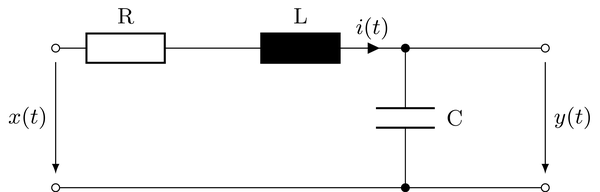
\includegraphics[width=0.5\textwidth]{../laplace_transform/lowpass.png}
\caption{Electric RLC circuit with current $i(t)$, input voltage $x(t)$
and output voltage $y(t)$.}
\label{fig:lowpass}
\end{figure}



%##############################################################################
\subsubsection{Ordinary Differential Equation (ODE)}
There is one current $i(t)$ flowing in the RLC circuit under discussion.
The corresponding current-voltage laws for the components are
$u_R(t) = R\,i(t)$,
$u_L = L\,\frac{\mathrm{d}i(t)}{\mathrm{d} t}$ and
$u_C(t) = \frac{1}{C} \, \int i(t) \mathrm{d}t$.
With these \eq{eq:KirchhoffLaw} is rewritten as
%
\begin{align}
L C \cdot \ddot{u}_C(t) + R C \cdot \dot{u}_C(t) + u_C(t) = u_0(t)
\end{align}
using
$\ddot{u}_C(t) = \frac{\mathrm{d}^2 u_C(t)}{\mathrm{d}t^2}$ and
$\dot{u}_C(t) = \frac{\mathrm{d} u_C(t)}{\mathrm{d}t}$
as temporal derivative notations.
%
With
the system input $x(t)$ and
the system output $y(t)$ this 2nd order, linear ODE with
constant coefficients is rewritten
\begin{align}
\label{eq:ODE_RLC}
L C \cdot \ddot{y}(t) + R C \cdot \dot{y}(t) + y(t) = x(t).
\end{align}



%##############################################################################
\subsubsection{Task}
The ODE in \eq{eq:ODE_RLC} with
$R = 3\,\nicefrac{\text{V}}{\text{A}}$,
$L=2\,\nicefrac{\text{V s}}{\text{A}}$,
$C=\frac{8}{25}\,\nicefrac{\text{A s}}{\text{V}}$
is to be solved for $t\geq 0$ and the cases
\begin{itemize}
\item[a)] $y_\text{particular}(t)$ when $x(t)=\delta(t)$
\item[b)] $y(t) = y_\text{hom}(t)+y_\text{particular}(t)$ when
$x(t)=1$ and initial conditions $\dot{y}(0) = 0$, $y(0)=0$
\item[c)] $y(t) = y_\text{hom}(t)+y_\text{particular}(t)$ when $x(t)=0$
and initial conditions $\dot{y}(0) = 2$, $y(0)=1$
\item[d)] $y(t) = y_\text{hom}(t)+y_\text{particular}(t)$ when $x(t)=1$
and initial conditions $\dot{y}(0) = 2$, $y(0)=1$
\item[e)] $y(t) = y_\text{hom}(t)+y_\text{particular}(t)$ when $x(t)=\sin(t)$
and initial conditions $\dot{y}(0) = 0$, $y(0)=0$
\end{itemize}
denoting the Dirac-Delta impulse $\delta(t)$.
%and Heaviside step function
%$\epsilon(t)= \{0\,\,\text{for}\,\,t < 0;\,\,\, 1\,\,\text{for}\,\,t \geq 0\}$.
%
For Dirac impulse initial conditions refer to $t=0-$ since excitation is at $t=0$.
For other signals, initial conditions refer to the exact time instance $t=0$,
excitation signals start at right limit $t=0+$.
%
The task shall be performed with help of the \textbf{fundamental system of solutions}
and and with the help of the \textbf{Laplace transform}.



%##############################################################################
%##############################################################################
\subsection{Preliminaries for Fundamental System of Solutions}



%##############################################################################
\subsubsection{Helping Variables}
Before solving any of the requested tasks, it is good scientific and engineering
practice to adapt the ODE for convenient handling and result's interpretation.
Thus (by some experience dealing with such problems and reading text books, cf.
\cite{LangeSigSys1}, \cite{Goeldner1987},  \cite{Oppenheim1997}, \cite{Strang2014}),
we introduce
\begin{equation}
\omega_0^2 = \frac{1}{L C} \rightarrow \omega_0 = \frac{1}{\sqrt{L C}}
\end{equation}
(this is the \textbf{resonance frequency} of the system when no damping would occur)
and
\begin{equation}
\sigma_0 = \frac{1}{2}\frac{R}{L},
\qquad
D = \frac{\sigma_0}{\omega_0}.
\end{equation}
(these are related to the \textbf{damping quality} of the system).
%
Furthermore,
\begin{equation}
\omega_D^2 = \omega_0^2 (1-D^2) \qquad \rightarrow \qquad \omega_D = \omega_0
\sqrt{1-D^2}
\end{equation}
becomes convenient for the case $\sigma_0^2 - \omega_0^2 < 0$.
We will later experience the usefulness of these helping variables.
For now, it is worth to note that $\omega_0$ and $\sigma_0$ intentionally share
\textbf{similarities} with the variable $s=\sigma + \im \omega$ used for the
\textbf{Laplace transform}.

By introducing the variables into \eq{eq:ODE_RLC}, we have nice formatted
\begin{align}
\label{eq:ODE_sigma0}
\boxed{
\frac{\ddot{y}}{\omega_0^2} + \frac{2 \sigma_0}{\omega_0^2} \dot{y} + y = x
}\,,
\end{align}
and
\begin{align}
\label{eq:ODE_D}
\boxed{
\frac{\ddot{y}}{\omega_0^2} + \frac{2 D}{\omega_0} \dot{y} + y = x}\,,
\end{align}
when omitting the temporal dependence $t$ in $y$ and $x$ for brevity.
%
This generalisation allows for discussion of the ODE's characteristics detached
from the underlying physical representation and helps for communication between
scientists and engineers with different job specialisation.



%##############################################################################
\subsubsection{Specific Parameters}
With the given values for the electric elements
$R = 3\,\nicefrac{\text{V}}{\text{A}}$,
$L=2\,\nicefrac{\text{V s}}{\text{A}}$,
$C=\frac{8}{25}\,\nicefrac{\text{A s}}{\text{V}}$
we can rewrite \eq{eq:ODE_RLC}
\begin{align}
\boxed{
(\frac{16}{25} \cdot \text{s}^2) \, \ddot{y} + (\frac{24}{25} \cdot \text{s})
\, \dot{y} + y = x.
}
\end{align}
Note that the straight letter s here represents the unit seconds, \textbf{not the Laplace
variable}, which is typeset as italic $s$.
%
The above variables have the quantities
\begin{equation}
\omega_0^2 = \frac{25}{16} \cdot \frac{\text{rad}^2}{\text{s}^2}
\rightarrow \omega_0 = \frac{5}{4} \cdot \frac{\text{rad}}{\text{s}}
\end{equation}
and
\begin{equation}
\sigma_0 = \frac{3}{4}\cdot \frac{\text{1}}{\text{s}}
\qquad D = \frac{3}{5}
\end{equation}
and since $\sigma_0^2 - \omega_0^2 = -1 \cdot \frac{1}{\text{s}^2}< 0\cdot \frac{1}{\text{s}^2}$
\begin{equation}
\omega_D = 1 \cdot \frac{\text{rad}}{\text{s}}.
\end{equation}
%
The chosen values for $R$, $L$, $C$ lead to convenient quantities, which is on
purpose for the upcoming manual calculus. For practical problems we should not
expect such nice numbers.
%
In the remainder we omit the physical units in the calculus, but it is always
useful to check if units are still meaningful after calculus.



%##############################################################################
\subsubsection{Homogeneous Solution}
\label{Sec:FundamentalSet}
The present 2nd order ODE can be solved by means of the
fundamental set of solutions
considering the eigenfunctions
\begin{align}
y = \mathrm{e}^{\lambda t}, \quad \lambda\in\mathbb{C}
\end{align}
of the system. Note the (intentional) similarity to $\mathrm{e}^{s t}$,
which is the integral kernel of the Laplace transform.
%
Derivatives with respect to time $t$ become (this is the nice part, why this
works at all)
\begin{align}
y = \mathrm{e}^{\lambda t},\quad
\dot{y} = \lambda \cdot \mathrm{e}^{\lambda t},\quad
\ddot{y} = \lambda^2 \cdot \mathrm{e}^{\lambda t}.
\end{align}
%
We insert these in \eq{eq:ODE_sigma0} with $x=0$, to obtain the
so called \textbf{homogeneous solution} $y_\text{hom}$, also denoted as
$y_h$.
Thus,
\begin{align}
\frac{1}{\omega_0^2} (\lambda^2 \cdot \mathrm{e}^{\lambda t}) +
\frac{2 \sigma_0}{\omega_0^2} (\lambda \cdot \mathrm{e}^{\lambda t}) +
\mathrm{e}^{\lambda t} = 0,\nonumber\\
\label{eq:CharEq}
(\underbrace{\frac{\lambda^2}{\omega_0^2} +
\frac{2 \sigma_0 \lambda}{\omega_0^2} + 1}_\text{characteristic equation})
\cdot \mathrm{e}^{\lambda t} = 0.
\end{align}
%
We are not able to force the left side of this equation to zero with the $\mathrm{e}^{\lambda t}$
function.
Thus, we calculate the zeros of the term within brackets, which is well known as
\textbf{characteristic equation}.
%
The zeros of this 2nd order polynomial are
\begin{align}
\label{lambda12}
\lambda_{1,2} = -\sigma_0 \pm \sqrt{\sigma_0^2 - \omega_0^2}.
\end{align}
%
The homogeneous solution $y_h$ depends on the characteristics
of the term $\sigma_0^2 - \omega_0^2$.
Three cases need to be considered.

\paragraph{Case I for Homogeneous Solution (Kriechfall, starke Dämpfung if $\sigma_0<0$)}
For
\begin{align}
\sigma_0^2 - \omega_0^2 > 0
\end{align}
the Ansatz reads
\begin{align}
y_h=
A \mathrm{e}^{\lambda_1 t} + B \mathrm{e}^{\lambda_2 t}
=
\mathrm{e}^{-\sigma_0 t} [A \mathrm{e}^{+t\,\sqrt{\sigma_0^2 - \omega_0^2}}
+ B \mathrm{e}^{-t\,\sqrt{\sigma_0^2 - \omega_0^2}}]
\end{align}
with the two constants $A$ and $B$ to be defined by the initial conditions
$\dot{y}(t)$ and $y(t)$ for a given $t$ (very often $t=0$)
of the the complete solution
$y(t) = y_\text{hom}(t)+y_\text{particular}(t)$.

\paragraph{Case II for Homogeneous Solution (Aperiodischer Grenzfall)}
For
\begin{align}
\sigma_0^2 - \omega_0^2 = 0
\end{align}
a double zero
\begin{align}
\lambda_{1} = \lambda_{2} = -\sigma_0
\end{align}
results for \eq{lambda12}.
Then the Ansatz reads
\begin{align}
y_h = \mathrm{e}^{-\sigma_0 t} [A t + B].
\end{align}

\paragraph{Case III for Homogeneous Solution (Schwingungsfall,
schwache Dämpfung if $\sigma_0<0$)}
\label{pg:caseIII}
For
\begin{align}
\sigma_0^2 - \omega_0^2 < 0,
\end{align}
the already introduced helping variable
\begin{align}
\omega_D^2 = \omega_0^2 - \sigma_0^2 > 0
\end{align}
rearranges \eq{lambda12} to
\begin{align}
\label{eq:lmb12_caseIII}
\lambda_{1,2} = -\sigma_0 \pm \sqrt{-\omega_D^2}
= -\sigma_0 \pm \mathrm{j}\,\omega_D,
\end{align}
yielding a complex conjugate zero pair.
Then the Ansatz reads (cf. case I)
\begin{align}
\label{eq:Ansatz_caseIIIkomplex}
\boxed{
y_h = A \mathrm{e}^{\lambda_1 t} + B \mathrm{e}^{\lambda_2 t}.
}
\end{align}
or (by using other $A$, $B$!)
\begin{align}
\label{eq:Ansatz_caseIIIsincos}
y_h = \mathrm{e}^{-\sigma_0 t}
\left[ A \sin(\omega_D t) + B \cos(\omega_D t)\right].
\end{align}
While \eq{eq:Ansatz_caseIIIkomplex} is more elegant to perform calculus,
\eq{eq:Ansatz_caseIIIsincos} directly reveals the \textbf{damped}
(parameter $\sigma_0$) sine and cosine \textbf{oscillations}
(with angular frequency $\omega_D$).
%
Case III covers the characteristics of the majority of practical systems
for signal processing.



%##############################################################################
\subsubsection{Inhomogeneous Solution}
Now, let the ODE be of form
\begin{align}
a \, \ddot{y} + b \, \dot{y} + c \, y = x.
\end{align}
with constant coefficients $a, b, c\in \mathbb{R}$.
%
There are different suitable approaches for solving such an ODE for
different inhomogeneities $x$.
We restrict our discussion to the most often asked cases.
We should check our math lecture notes for e.g. the method
\textit{variation of parameters / Variation der Konstanten} for a general
solution concept, cf. \cite{Burg2013}.

\paragraph{Polynomial Function}
The particular solution $y_p$ for the inhomogeneous ODE with
polynomial $x = P_n(t)$ of degree $n$
(for example $x = p_n t^n + p_{n-1} t^{n-1} + ... +p_0$)
requires the Ansatz
\begin{align}
y_p =
\begin{cases}
Q_n(t)&\quad a\neq 0, c\neq 0\\
t Q_n(t)&\quad a\neq 0, b\neq 0, c=0\\
t^2 Q_n(t)&\quad a\neq 0, b=0, c=0
\end{cases}
\end{align}
and solving for the coefficients $q_n, q_{n-1},...,q_0$ by comparing
coefficients in
\begin{align}
a \, \ddot{y}_p + b \, \dot{y}_p + c \, y_p = x.
\end{align}

\paragraph{Exponential Function (i.e. Eigenfunctions of the ODE)}
The particular solution $y_p$ for the inhomogeneous ODE with
$x = \e^{s_x t}$
requires the Ansatz
\begin{align}
y_p =
\begin{cases}
A \cdot \e^{s_x t}&\quad \text{if} \quad  s_x \notin \lambda_{1,2}\\
A t \cdot \e^{s_x t}&\quad \text{if} \quad s_x \in \lambda_{1 \text{ or } 2}\\
A t^2 \cdot \e^{s_x t}&\quad \text{if} \quad s_x \in \lambda_{1 \text{ and } 2}
\end{cases}
\end{align}
and solving for the coefficient $A$ by comparing coefficients.

\paragraph{Cosine / Sine Functions (i.e. Special Case of ODE's Eigenfunctions)}
\label{Sec:CosSineAnsatzInhomo}
The particular solution $y_p$ for the inhomogeneous ODE with
$x=\sin(\omega_x t)$ or $x=\cos(\omega_x t)$
requires the Ansatz
\begin{align}
y_p =
\begin{cases}
A \cdot \cos(\omega_x t) + B \cdot \sin(\omega_x t)&\quad \text{if}
\quad \im \omega_x \notin \lambda_{1,2}\\
A t \cdot \cos(\omega_x t) + B t \cdot \sin(\omega_x t)&\quad \text{if}
\quad \im \omega_x \in \lambda_{1,2}
\end{cases}
\end{align}
and solving for the coefficients $A, B$ by comparing coefficients.



%##############################################################################
\subsubsection{Full ODE Solution}
The full solution of an ODE is the superposition of the homogeneous solution
and inhomogeneous (particular) solution
\begin{align}
y(t) = y_\text{hom}(t)+y_\text{particular}(t) \qquad \rightarrow \qquad
y = y_h + y_p
\end{align}
and then resolving for the initial conditions $\dot{y}(t)$ and $y(t)$ for a
given $t$ (very often $t=0$) to obtain the specific solution $y$.



%##############################################################################
%##############################################################################
\subsection{Solutions Using Fundamental System}



%##############################################################################
\subsubsection{Task a) with Fundamental System / Impulse Response}
We shall solve
\begin{align}
\frac{16}{25} \ddot{y} + \frac{24}{25} \dot{y} + y = \delta(t)
\end{align}
for the particular solution $y_p$ in the time domain.

%
A brilliant didactical approach tailored for engineers to solve this task is
found in \cite{Strang2014}.
%
In short, the \textbf{particular solution} $y_p(t)$ of this equation
with \textbf{Dirac impulse excitation} is named the \textbf{Green's function} $g(t)$.
%
When the homogeneous solutions of the ODE are known, the Green's function can be found
by variation of parameters.
Making use of the important sifting property
$\int\limits_{-\infty}^{+\infty} \delta(t-t_0) \cdot f(t) \, \mathrm{d} t \stackrel{\mathrm{def}}= f(t_0)$
becomes a vital part when doing this.
%
However, we will not go into detail here, cf. \cite[p.133]{Strang2014} instead.
%
The important part of the story is:
Once $g(t)$ is known,
the \textbf{particular solution} $y_p$ \textbf{for any other inhomogeneity}
$x(t)$ can be derived with the \textbf{convolution} operation
$y_p(t) = x(t) * g(t)$.
%
This constitutes a fundamental (if not the most important) theorem for ODEs.
%
For our discussed ODEs in signal and
system theory (where we only handle time dependence), we call the Green's
function $g(t)$ typically the \textbf{impulse response} $h(t)$ of the
\textbf{LTI system} and use the convolution $y_p(t) = x(t) * h(t)$.

\textbf{Important detail}: Actually the problem
$\frac{16}{25} \ddot{h}(t) + \frac{24}{25} \dot{h}(t) + h(t) = \delta(t),\,\,\,
\dot{h}(0-)=0,\,\,\,h(0-)=0$
solves for the impulse response, where we need the \textbf{left sided}
limit $t=0-$, since the Dirac impulse excites at $t=0$.
%
This proof is a little bit off-topic due to lack of time.
%
Instead, we can use the particular solution only by keeping in
mind that the system was in rest before excitation.

Said that, we can make our life even more convenient, since according to
\cite[p.97]{Strang2014},
the \textbf{Green's function is also found by the homogeneous solution}
(instead of Dirac excitation)
\textbf{and new specific initial conditions}.
In general for a 2nd order ODE this means
%\begin{align}
$a \, \ddot{y} + b \, \dot{y} + c \, y = 0,
\quad y(0)=0,
\quad \dot{y}(0)=\frac{1}{a}$,
%\end{align}
and thus for our specified example
\begin{align}
\frac{16}{25} \ddot{y} + \frac{24}{25} \dot{y} + y = 0,
\quad y(0)=0,
\quad \dot{y}(0)=\frac{25}{16}
\end{align}
for $t\geq 0$.
%
Feel free to explore the solution by usage of \url{https://www.wolframalpha.com}
with the input \verb|16/25*y’’(t)+24/25*y’(t)+y(t)=0, y(0)=0, y'(0)=25/16|
or with other tools that can handle symbolic math on a computer.
%
We are going to calculate this manually in the following.
%


\paragraph{Homogeneous Solution}
\label{Sec:TaskaHomo}
First, we need the homogeneous solution of the ODE for this subtask.
%
We will also need this in general, so it is anyway a good idea to calculate
this first.
%
According to Sec. \ref{Sec:FundamentalSet} the characteristic equation for the
ODE is \eq{lambda12}
\begin{align}
\lambda_{1,2} = -\sigma_0 \pm \sqrt{\sigma_0^2 - \omega_0^2}.
\end{align}
and with the chosen quantities, we get
\begin{align}
\lambda_{1,2} = -\frac{3}{4} \pm \im,
\end{align}
i.e. a complex conjugate zero pair with intentionally very simple numbers.
Thus, we deal with \textbf{case III} (page \pageref{pg:caseIII})
for the homogeneous solution, this is the case of \textbf{damped oscillation}.
The corresponding zero pair is depicted in Fig.~\ref{fig:sketch_lambda_plane},
left.
%
Repeating \eq{eq:lmb12_caseIII}
$\lambda_{1,2} = -\sigma_0 \pm \mathrm{j}\omega_D$,
we identify $\sigma_0 = \frac{3}{4}$ and $\omega_D = 1$.
Repeating \eq{eq:Ansatz_caseIIIkomplex}
$y_h = A \mathrm{e}^{\lambda_1 t} + B \mathrm{e}^{\lambda_2 t}$,
we therefore have to deal with
\begin{align}
y_h = A \, \mathrm{e}^{(-\frac{3}{4}+\im)\,t} + B \, \mathrm{e}^{(-\frac{3}{4}-\im)\,t},
\end{align}
and since $y_p=0$
\begin{align}
y = y_h + y_p = A \, \mathrm{e}^{(-\frac{3}{4}+\im)\,t} + B \, \mathrm{e}^{(-\frac{3}{4}-\im)\,t}.
\end{align}

\paragraph{Initial Conditions}
\label{Sec:TaskaInitCond}
The initial conditions $y(0)=0$ and $\dot{y}(0)=\nicefrac{25}{16}$ require to find
the derivative
\begin{align}
\dot{y} =
(-\frac{3}{4}+\im) A \, \mathrm{e}^{(-\frac{3}{4}+\im)\,t} +
(-\frac{3}{4}-\im) B \, \mathrm{e}^{(-\frac{3}{4}-\im)\,t}.
\end{align}
%
The ease of performing this derivation makes the Ansatz \eq{eq:Ansatz_caseIIIkomplex}
more elegant than \eq{eq:Ansatz_caseIIIsincos}.
%
However, we now have slightly more effort to find the coefficients $A$ and $B$,
but it is actually more enlightening, how our final result evolves.
%
Applying the initial conditions yields
%
\begin{align}
y(0) = 0 = A + B
\qquad
\dot{y}(0) = \nicefrac{25}{16} =
(-\frac{3}{4}+\im) \, A + (-\frac{3}{4}-\im) \, B
\end{align}
Thus, comparing coefficients and using one Euler identity
$\sin(x) = \frac{\e^{\im x}-\e^{-\im x}}{2\im}$
\begin{align}
A = \frac{\nicefrac{25}{16}}{2\im}\qquad B = -\frac{\nicefrac{25}{16}}{2\im}
\quad\rightarrow\quad
y = y_h + y_p =
 \frac{\nicefrac{25}{16}}{2\im} \, \mathrm{e}^{(-\frac{3}{4}+\im)\,t}
-\frac{\nicefrac{25}{16}}{2\im} \, \mathrm{e}^{(-\frac{3}{4}-\im)\,t},
\end{align}
yields the \textbf{impulse response} of the 2nd order system / ODE under discussion
\begin{align}
\boxed{
h = y_\text{Task a} = \nicefrac{25}{16} \cdot \mathrm{e}^{-\frac{3}{4} t} \sin(t) \qquad t\geq0
}\,.
\end{align}



%##############################################################################
\subsubsection{Task b) with Fundamental System / Step Response}
We shall solve
\begin{align}
\frac{16}{25} \ddot{y} + \frac{24}{25} \dot{y} + y = 1, \quad
\dot{y}(0) = 0,\quad y(0)=0
\end{align}
for $y$ with the Ansatz of fundamental set of solutions.

\paragraph{Inhomogeneous Solution}
The source term $x(t\geq 0+)=1$ exhibits unit
amplitude over time. This can be stated as the most simple polynomial $p_0=1$.
Thus, the polynomial Ansatz $y_p = q_0$ leads to
\begin{align}
\frac{16}{25} \ddot{y}_p + \frac{24}{25} \dot{y}_p + y_p = 1
\rightarrow q_0 = 1 \rightarrow  y_p = 1.
\end{align}

\paragraph{Specific Solution with Initial Conditions}
The superposition of the homogeneous (this time we use the sin/cos-Ansatz
\eq{eq:Ansatz_caseIIIsincos} for demonstration purpose) and the inhomogeneous
solution is
\begin{align}
\label{eq:SpecificyTaskb}
y = y_h + y_p = \underbrace{
\mathrm{e}^{-\frac{3}{4} t} \cdot
\left[ A \sin(t) + B  \cos(t)\right]}_{y_h} +\underbrace{1}_{y_p}.
\end{align}
The initial condition $\dot{y}(0) = 0$ again requires to find the derivative
\begin{align}
\dot{y}
=
-\frac{3}{4}\mathrm{e}^{-\frac{3}{4} t} \cdot
\left[ A \sin(t) + B \cos(t)\right]
+
\mathrm{e}^{-\frac{3}{4} t} \cdot
\left[ A \cos(t)  - B \sin(t)\right].
\end{align}
The initial condition $\dot{y}(0) = 0$ yields
\begin{align}
0 = -\frac{3}{4}\cdot B + A \rightarrow A = \frac{3}{4}\cdot B.
\end{align}
The initial condition ${y}(0) = 0$ yields
\begin{align}
0 = B  + 1 \rightarrow B = -1.
\end{align}
The resulting coefficients
\begin{align}
A = -\frac{3}{4}\qquad B = -1
\end{align}
are inserted into \eq{eq:SpecificyTaskb}
\begin{align}
\boxed{
h_\epsilon = y_\text{Task b} =
1 - \mathrm{e}^{-\frac{3}{4} t} \cdot
\left(\frac{3}{4} \sin(t) + \cos(t)\right) \qquad t \geq 0
}\,,
\end{align}
giving the final result for task b) with $h_\epsilon(t\to\infty) = 1$.

In Fig.~\ref{fig:step_response_parts} the solution $y_\text{Task b}$ is depicted
as the thick, non-dashed orange graph. It results from the superposition of the
functions
a) unit amplitude (black),
b) exponentially damped, negative sine (green, diamonds),
c) exponentially damped, negative cosine (red, stars).
In grey colour, the pure sine and cosine functions with negative amplitude,
as well as the exponential
damping with different initial amplitude are indicated.

\begin{figure}[h!]
\centering
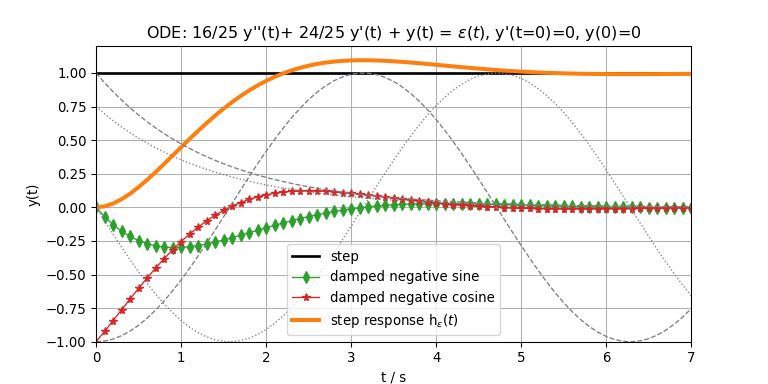
\includegraphics[width=0.75\textwidth]{../laplace_transform/step_response_parts}
\caption{Response of task b for ODE under discussion.}
\label{fig:step_response_parts}
\end{figure}

Feel free to double check this solution at Wolfram Alpha with input
\begin{verbatim}
16/25*y''(t)+24/25*y'(t)+y(t)=1,       y'(0)=0, y(0)=0
16/25*y''(t)+24/25*y'(t)+y(t)=Step[t], y'(0)=0, y(0)=0
\end{verbatim}




%##############################################################################
\subsubsection{Task a) Revisited with Fundamental System / Impulse Response}
%
The Heaviside step function
\begin{equation}
\epsilon(t) =
\begin{cases}
  0 & t\leq 0-\\
  1 & t\geq 0+
\end{cases}
\end{equation}
and
the Dirac impulse $\delta(t)$ are related by
\begin{align}
\dot{\epsilon}(t) = \delta(t).
\end{align}
In fact, in task a and b we just derived the impulse response $h(t)$ and step response
$h_\epsilon(t)$ of the ODE, respectively.
%
We can also relate the step and impulse response by
\begin{align}
\dot{h_\epsilon}(t) = h(t).
\end{align}
%
The \textbf{temporal derivative of the step response} $h_\epsilon=y_\text{Task b}$
\textbf{yields the impulse response} $h$.
Thus, for the step response
\begin{align}
h_\epsilon = y_\text{Task b} =
1 - \mathrm{e}^{-\frac{3}{4} t} \cdot
\left( \frac{3}{4} \sin(t) + \cos(t)\right)
\end{align}
the derivative is the impulse response
\begin{align}
h = \dot{h_\epsilon} = \dot{y}_\text{Task b} =
 - (-\frac{3}{4})\,\mathrm{e}^{-\frac{3}{4} t} \cdot
\left( \frac{3}{4} \sin(t) + \cos(t)\right)
- \mathrm{e}^{-\frac{3}{4} t} \cdot
\left( \frac{3}{4} \cos(t) - \sin(t)\right).
\end{align}
Rearranging yields the expected result identical to task a
\begin{align}
\boxed{
h = y_\text{Task a} = \frac{25}{16} \mathrm{e}^{-\frac{3}{4} t} \sin(t) \qquad t\geq 0
}\,.
\end{align}
%
In Fig. \ref{fig:impulse_step_response} the impulse response is depicted as
the dashed blue graph, whereas the step response is plotted in thick
orange again.
The impulse response is a weighted and exponentially damped sine function
with $h(t\to\infty) = 0$.

\begin{figure}[h!]
\centering
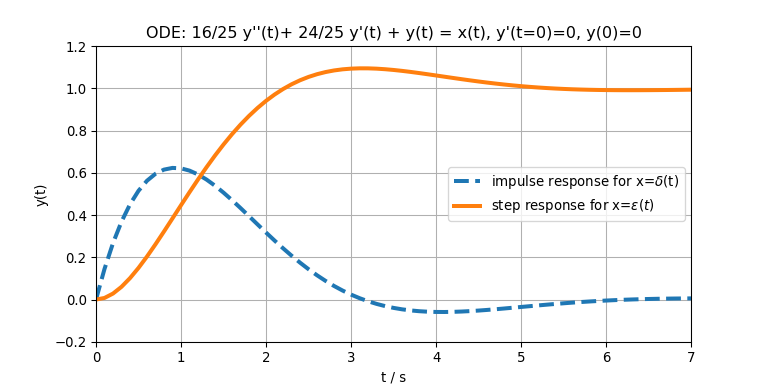
\includegraphics[width=0.75\textwidth]{../laplace_transform/impulse_step_response}
\caption{Impulse response (task a, blue, dotted) and step response (task b, orange, thick)
of the ODE under discussion.}
\label{fig:impulse_step_response}
\end{figure}

Feel free to verify that Wolfram Alpha returns the particular solution to the
input
\begin{verbatim}
16/25*y''(t)+24/25*y'(t)+y(t)=DiracDelta[t]
\end{verbatim}
precisely identical to the manually calculated impulse response.



%##############################################################################
\subsubsection{Task c) with Fundamental System}
Now, we shall solve
\begin{align}
\frac{16}{25} \ddot{y} + \frac{24}{25} \dot{y} + y = 0,
\quad \dot{y}(0) = 2,\quad y(0)=1
\end{align}
for $y$.
%
Since $y_p=0$, we can immediately adapt the solution of Sec.
\ref{Sec:TaskaHomo} and \ref{Sec:TaskaInitCond} as
%
\begin{align}
y_h + y_p = y =& A \, \mathrm{e}^{(-\frac{3}{4}+\im)\,t} + B \, \mathrm{e}^{(-\frac{3}{4}-\im)\,t}\\
\dot{y} =&
(-\frac{3}{4}+\im) A \, \mathrm{e}^{(-\frac{3}{4}+\im)\,t} +
(-\frac{3}{4}-\im) B \, \mathrm{e}^{(-\frac{3}{4}-\im)\,t}
\end{align}
%
Applying the initial conditions yields
%
\begin{align}
\dot{y}(0) = 2 =
(-\frac{3}{4}+\im) A+
(-\frac{3}{4}-\im) B
\qquad
y(0) = 1 = A + B.
\end{align}
Thus, the coefficients become
\begin{align}
A = \frac{1}{2} + \frac{11}{8\im}\qquad B = 1-A = \frac{1}{2} - \frac{11}{8\im}.
\end{align}
%
Inserting these and applying the Euler identities
$\cos(x) = \frac{\e^{\im x}+\e^{-\im x}}{2}$,
$\sin(x) = \frac{\e^{\im x}-\e^{-\im x}}{2\im}$
yields
\begin{align}
\boxed{
y_\text{Task c} = \mathrm{e}^{-\frac{3}{4} t} \cdot
\left( \frac{11}{4} \sin(t) + \cos(t)\right) \qquad t\geq 0
}\,.
\end{align}
In Fig.~\ref{fig:initial_conditions_response_parts} the brown graph depicts the
response $y_\text{Task c}$, which is decaying to zero since the inductor $L$ and capacitor $C$ are
just discharging. As typical for such ODEs, again
weighted and exponentially damped cosine (red, stars) and sine (green, diamonds)
function are superimposed.

\begin{figure}[h!]
\centering
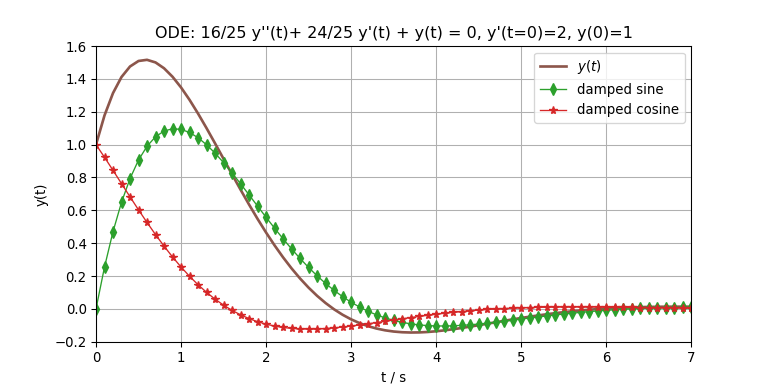
\includegraphics[width=0.75\textwidth]{../laplace_transform/initial_conditions_response_parts}
\caption{Response of task c for the ODE with initial conditions but no external input.}
\label{fig:initial_conditions_response_parts}
\end{figure}

Feel free to double check this solution at Wolfram Alpha with input
\begin{verbatim}
16/25*y''(t)+24/25*y'(t)+y(t)=0, y'(0)=2, y(0)=1
\end{verbatim}



%##############################################################################
\subsubsection{Task d) with Fundamental System}
In this task we shall solve
\begin{align}
\frac{16}{25} \ddot{y} + \frac{24}{25} \dot{y} + y = 1, \quad
\dot{y}(0) = 2,\quad y(0)=1
\end{align}
for $y$.
%
This task is the \textbf{superposition} of the solution from \textbf{task b} (exterior source
but vanishing initial conditions) and the solution of \textbf{task c} (no exterior
source, but initial conditions). Thus, we should expect
\begin{align}
&y_\text{Task d} =
y_\text{Task b} +
y_\text{Task c} = 1 + 2\mathrm{e}^{-\frac{3}{4} t} \sin(t) = \nonumber\\
&\left[1 - \mathrm{e}^{-\frac{3}{4} t} \cdot
\left( \frac{3}{4} \sin(t) + \cos(t)\right)\right]
+\left[\mathrm{e}^{-\frac{3}{4} t} \cdot
\left( \frac{11}{4} \sin(t) + \cos(t)\right)\right].
\end{align}
%
In order to reassure this result, we can start with \eq{eq:SpecificyTaskb} from
task b and rearrange this for the differing initial conditions:
The superposition of the homogeneous and inhomogeneous solution is
\begin{align}
y = y_h + y_p = \underbrace{
\mathrm{e}^{-\frac{3}{4} t} \cdot
\left( A \sin(t) + B \cos(t)\right)}_{y_h} + \underbrace{1}_{y_p}
\end{align}
Again, derivation with respect to time is
\begin{align}
\dot{y}
=
-\frac{3}{4}\,\mathrm{e}^{-\frac{3}{4} t} \cdot
\left( A \sin(t) + B \cos(t)\right)
+
\mathrm{e}^{-\frac{3}{4} t} \cdot
\left( A \cos(t)  - B \sin(t)\right).
\end{align}
The initial condition $\dot{y}(0) = 2$ yields
\begin{align}
2 = -\frac{3}{4}\cdot B + A \rightarrow A = 2 +  \frac{3}{4}\cdot B.
\end{align}
The initial condition ${y}(0) = 1$ yields
\begin{align}
1 = B  + 1 \rightarrow B = 0.
\end{align}
Thus,
\begin{align}
A = 2\qquad B = 0
\end{align}
inserted
\begin{align}
\boxed{
y_\text{Task d} =
1+\mathrm{e}^{-\frac{3}{4} t}
\, 2 \sin(t)\qquad t \geq 0
}
\end{align}
leads to the final result for task d) as expected.
%
\begin{figure}[b!]
\centering
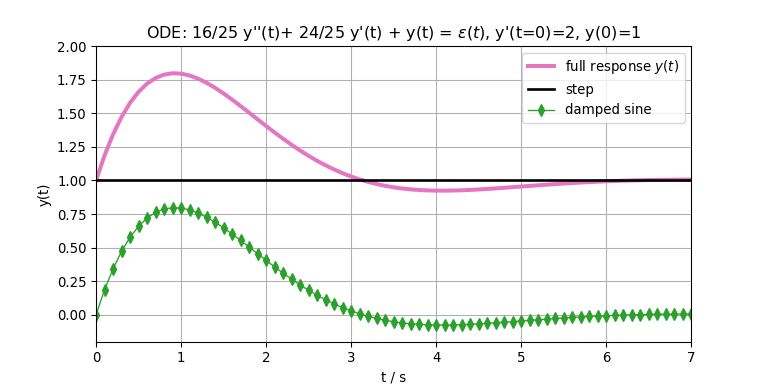
\includegraphics[width=0.75\textwidth]{../laplace_transform/response_full}
\caption{Response of task d for the ODE with initial conditions and step input.}
\label{fig:response_full}
\end{figure}
%
In Fig.~\ref{fig:response_full} the response $y_\text{Task d} $ is depicted as
magenta graph. This is the result of the superposition of the Heaviside step
function and an exponentially damped, weighted sine function.
The final result asymptotically converges to unit amplitude.
%
This is expected: as the effects of initial conditions have been vanished at $t\to\infty$
the external excitation of the step function is the dominant part for the system
response.
%
We can see this in the equations: $y_\text{Task d}(t\to\infty) = y_\text{Task b}(t\to\infty)$

Feel free to double check this solution at Wolfram Alpha with input
\begin{verbatim}
16/25*y''(t)+24/25*y'(t)+y(t)=1, y'(0)=2, y(0)=1
\end{verbatim}





%##############################################################################
\subsubsection{Task e) with Fundamental System}
In this task we shall solve
\begin{align}
\label{eq:InHomoODE_sin}
\frac{16}{25} \ddot{y} + \frac{24}{25} \dot{y} + y = \sin(t), \quad
\dot{y}(0) = 0,\quad y(0)=0
\end{align}
for $y$.
%
We already know the homogeneous solution
$y_h = \mathrm{e}^{-\frac{3}{4} t} \cdot
\left[ A \sin(t) + B \cos(t)\right]$.
%
The inhomogeneity in this case can be solved with the Ansatz (cf.
Sec. \ref{Sec:CosSineAnsatzInhomo})
\begin{align}
y_p = C \sin(t) + D \cos(t).
\end{align}
Inserting this into \eq{eq:InHomoODE_sin}, the
coefficients are solved to (still somehow nice numbers, but we see that this can
become a mess for even more complicated excitations
)
\begin{align}
C = \frac{25}{73}\qquad D = -\frac{200}{219}.
\end{align}
%
The solution then becomes
\begin{align}
y = y_h + y_p = \underbrace{\mathrm{e}^{-\frac{3}{4} t} \cdot
\left[ A \sin(t) + B \cos(t)\right]}_{\text{damped solution} \, y_h}+
\underbrace{\frac{25}{73} \sin(t) - \frac{200}{219} \cos(t)}_{\text{oscillating solution} \, y_p}.
\end{align}
By considering the initial conditions the remaining unknown coefficients solve to
\begin{align}
A = \frac{25}{73}\qquad B = \frac{200}{219}
\end{align}
giving the final result
\begin{align}
\boxed{
y_\text{Task e} = \frac{25}{73} \mathrm{e}^{-\frac{3}{4} t} \sin(t) +
\frac{200}{219} \mathrm{e}^{-\frac{3}{4} t} \cos(t) +
\frac{25}{73} \sin(t) -
\frac{200}{219} \cos(t) \qquad t\geq 0
}\, ,
\end{align}
%
\begin{figure}[h!]
\centering
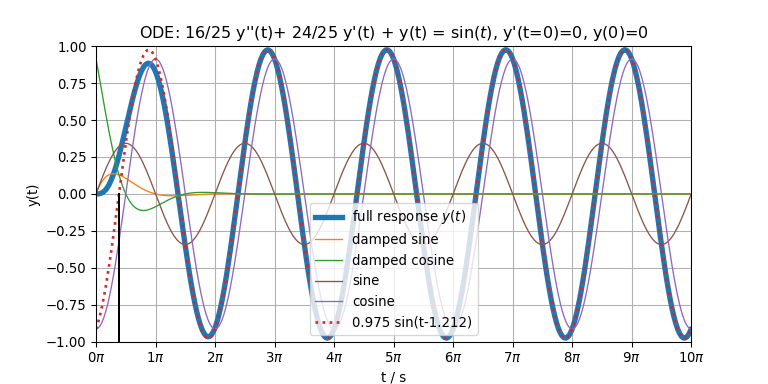
\includegraphics[width=0.75\textwidth]{../laplace_transform/sine_excitation_response}
\caption{Response of task e for the ODE with zero initial conditions and
$\sin(t)$ input.}
\label{fig:sine_excitation_response}
\end{figure}

The response is depicted in Fig.~\ref{fig:sine_excitation_response} in
thick/blue.
It results from the superposition of a) weighted and \textbf{exponentially damped}
sine and cosine functions (yellow and green graphs) and b) weighted but \textbf{undamped}
sine and cosine functions (brown and purple graphs).

\subsubsection{Steady State of the System}
%
In this example it is important to realise that the initial conditions
(exponentially damped sine and cosine) contribute
to the system response only up to approximately $t=2\pi$
seconds, i.e. in the first period $T=\frac{2\pi}{\omega_D}=2\pi$ of the
excitation's frequency here.
%
For times $t\gg2\pi$ seconds the system response is determined by the
undamped sine and cosine functions, yielding a system response of
\begin{align}
\label{eq:steadystate_timedomain}
y(t\gg 2\pi, t\to\infty) = \frac{25}{3 \sqrt{73}}\cdot
\sin\left(t-\tan^{-1}
\left[\frac{\nicefrac{200}{219}}{\nicefrac{25}{73}}\right]\right),
\end{align}
depicted as the red dotted graph in Fig.~\ref{fig:sine_excitation_response}.
This constitutes the so called \textbf{steady-state} of the system response
for $t\to\infty$.
For that, we see that the excitation signal $x=\sin(t)$ is altered in amplitude
(very subtle damping of about 0.975) and
a time delay (in terms of phase: about -70 degrees or about $-0.386 \pi$ in
radian), cf. the black line indicator in the figure.
Note that $\frac{\nicefrac{200}{219}}{\nicefrac{25}{73}} = \nicefrac{8}{3}$ again
results in simple numbers for the chosen example. We will rather not see such
for real practical problems.

The two parameters in the
\textbf{steady state}---\textbf{the amplitude and the phase offset}---and
their specific quantities are very important for the
interpretation of ODEs as LTI systems. Each excitation frequency has its own
quantity set, yielding frequency dependent system characteristics.
We will deal with it in detail when discussing ODEs in Laplace domain.
%
The so called Bode plot or \textbf{Bode diagram} is one important tool
to visualize amplitude and phase over frequency in approximated manner.
%
Nowadays, exact computation of amplitude and phase over frequency is convenient
using computers.

Feel free to double check this solution at Wolfram Alpha with input
\begin{verbatim}
16/25*y''(t)+24/25*y'(t)+y(t)=Sin[t], y'(0)=0, y(0)=0
\end{verbatim}





%##############################################################################
\subsection{Preliminaries for Laplace Transform}
We should now study the problem with the help of the Laplace transform.
For the chosen ODE and input signals the calculus effort is about the same,
however for slightly more complicated cases, the approach via Laplace transform
is often the more convenient approach for the solution.
%
For instance, Laplace transform is more powerful, when the \textbf{steady state}
system response for oscillations \textbf{at many different frequencies} is
searched for.
%
Instead of solving each individual problem with the approach that we took before,
the problem is conveniently solved by means of the \textbf{transfer function},
which stores amplitude and phase offset for each arbitrary oscillation frequency.
%
We will discover this, when solving tasks a) to e) with the help of the Laplace
transform. The solutions must be of course identical to these we have found so far.

To obtain the time functions the inverse Laplace function needs to be calculated.
%
We do not need to use the complex integral and application of the
\textbf{residue theorem}
here in SigSys, but rather make use of \textbf{correspondence tables for Laplace transforms}.
%
The English and German textbooks
\cite{Strang2010,Strang2014,GirodRabensteinStenger2007,Girod2001,Oppenheim1997,Fliege1991,
Goeldner1987,LangeSigSys1,Wunsch1972}
can be considered classics and cover the Laplace transform very well for our
purpose.




%##############################################################################
\subsubsection{Laplace Transform Fundamentals}
The Laplace transform pair reads
\begin{align}
Y(s) = \mathcal{L}\{y(t)\}= \int\limits_{-\infty}^{\infty} y(t) \e^{-s t}
\mathrm{d} t\qquad
y(t) = \mathcal{L}^{-1}\{Y(s)\}= \frac{1}{2\pi\im}\int
\limits_{\sigma-\im \infty}^{\sigma+\im\infty} Y(s) \e^{+s t} \mathrm{d} s.
\end{align}
We use the operators
$y(t) \quad \laplace \quad Y(s)$ and
$Y(s) = \mathcal{L}\{y(t)\}$
to indicate forward Laplace transform.
We use the operators
$Y(s) \quad \Laplace \quad y(t)$ and
$y(t) = \mathcal{L}^{-1}\{Y(s)\}$
to indicate inverse Laplace transform.

To make the Laplace transform helpful for solving ODEs, we first reconsider
that the Laplace transform is linear, i.e. it preserves scaling and
superposition in both signal domains
\begin{align}
A y_1(t) + B y_2(t) \quad \laplace \quad A Y_1(s) + B Y_2(s).
\end{align}
The second, fundamental important characteristics of the Laplace transform is
\begin{align}
\mathcal{L}\{\frac{\mathrm{d}^n y(t)}{\mathrm{d} t^n}\}=
s^n Y(s) - \sum_{k=1}^{n} s^{n-k} \cdot
\frac{\mathrm{d}^{k-1} y(t)}{\mathrm{d} t^{k-1}}\bigg|_{t=0},
\end{align}
The temporal derivation operation will be transformed to a multiplication
operation with Laplace variable $s$ (\textbf{differential equations} essentially \textbf{become
algebraic equations}, that is the key idea and a special case of
so called operator theory, we have seen a similar concept already for the
characteristic polynomial).
%
For typical systems up to 2nd order, we will need
\begin{align}
\label{eq:Laplace0thd}
\boxed{\mathcal{L}\{{y(t)}\} = Y(s)},
\end{align}
\begin{align}
\label{eq:Laplace1std}
\mathcal{L}\{\frac{\mathrm{d} y(t)}{\mathrm{d} t}\}=
s \cdot Y(s) - \sum_{k=1}^{1} s^{1-k} \cdot
\frac{\mathrm{d}^{k-1} y(t)}{\mathrm{d} t^{k-1}}\bigg|_{t=0}
= \boxed{\mathcal{L}\{\dot{y}\} = s \cdot Y(s) - y(0)}
\end{align}
and
\begin{align}
\label{eq:Laplace2ndd}
\mathcal{L}\{\frac{\mathrm{d}^2 y(t)}{\mathrm{d} t^2}\}=
s^2 \cdot Y(s) - \sum_{k=1}^{2} s^{2-k} \cdot
\frac{\mathrm{d}^{k-1} y(t)}{\mathrm{d} t^{k-1}}\bigg|_{t=0}
= \boxed{\mathcal{L}\{\ddot{y}\} = s^2 \cdot Y(s) - s \cdot y(0) - \dot{y}(0)}\,.
\end{align}

Note the \textbf{application of the initial conditions} in these transform rules!

%##############################################################################
\subsubsection{Algorithm for Solving ODEs via Laplace Transform}

Solving an ODE problem via the indirect way of Laplace transform is then as follows
\begin{itemize}
\item[1.] transform the ODE equation to the Laplace domain by applying rules of linearity and
derivatives
\item[2.] insert the initial conditions of $y(0)$  and $\dot{y}(0)$ and ...
(if they are zero, actually the additional terms immediately become zero,
this is very nice)
\item[3.] find the Laplace transform $X(s)$ of inhomogeneity $x(t)$ and insert
it (note that we are most often interested in $x(t)=\delta(t)$,
$x(t)=\epsilon(t)$, $x(t)=\exp(s_1 t)$ with $s_1\in\mathbb{C}$
as they tell us the most interesting things of the ODE)
\item[4.] reorganize the transformed equation for $Y(s)$
\item[5.] perform \textbf{inverse transformation} $y(t) = \mathcal{L}^{-1}\{Y(s)\}$
by means of either \textbf{partial fraction decomposition} and usage of
\textbf{transform tables}
or if this fails by means of the residue theorem...if this even fails we have a
very delicate problem at hand.
\footnote{For many systems we deal with in engineering,
someone very likely calculated the inverse Laplace transform already and we
might find it in formularies, list of integrals and textbooks.
So before trying to solve the integral of the inverse Laplace transform
manually, try to find the tabulated solution.
Though, very often the solution must be tweaked to fit into the tabulated
transforms.
Anyway, deriving solutions with residue theorem by our own is a
good exercise and enlightening.}
\end{itemize}

We aim at \textbf{right-sided}, and more specifically \textbf{causal systems and signals}.
Thus the region of convergence (ROC) is placed right of the most right pole of a
Laplace transform's function.
%
A stable LTI system requires poles only left of the $\Im(s)$-axis, i.e. only in
the left half of the $s$-plane.
%
This inherently implies, that $\Im(s)$-axis is part of the region of convergence (ROC),
and we can evaluated the frequency response of the system.

%##############################################################################
\subsubsection{Laplace Transform of the 2nd Order Linear ODE with Constant Coefficients}
The ODE under discussion is still \eq{eq:ODE_sigma0}
\begin{align}
\frac{\ddot{y}}{\omega_0^2} + \frac{2 \sigma_0}{\omega_0^2} \dot{y} + y = x
\end{align}
for which task a) to e) are to be solved by means of Laplace transform.
The general Ansatz valid for all tasks is sketched here.
%
First, considering linearity (scaling, superposition) yields
\begin{align}
\frac{1}{\omega_0^2} \ddot{y} +
\frac{2 \sigma_0}{\omega_0^2} \dot{y} + y = x
\quad \laplace \quad
\frac{1}{\omega_0^2} \mathcal{L}\{\ddot{y}\} +
\frac{2 \sigma_0}{\omega_0^2} \mathcal{L}\{\dot{y}\} + \mathcal{L}\{y\} =
\mathcal{L}\{x\}.
\end{align}
%
Second, the temporal derivative rules \eq{eq:Laplace0thd}, \eq{eq:Laplace1std}
and \eq{eq:Laplace2ndd} are applied to functions $y$ and $x$ yielding
\begin{align}
\frac{1}{\omega_0^2} \left[ s^2 \cdot Y(s) - s \cdot y(0) - \dot{y}(0)\right]  +
\frac{2 \sigma_0}{\omega_0^2} \left[ s \cdot Y(s) - y(0) \right] + Y(s) = X(s).
\end{align}
%
Rearranging for $Y(s)$ yields (we must \textbf{savely distinguish} between $Y$, $y$ and $\dot{y}$
in that equation, pay special attention with handwriting!)
\begin{align}
Y(s) = \frac{X(s)}{\frac{1}{\omega_0^2} s^2 +
\frac{2 \sigma_0}{\omega_0^2} s + 1}
+ \frac{\frac{1}{\omega_0^2} s \cdot y(0) + \frac{2 \sigma_0}{\omega_0^2} \cdot y(0) +
\frac{1}{\omega_0^2} \cdot \dot{y}(0)}{\frac{1}
{\omega_0^2} s^2 + \frac{2 \sigma_0}{\omega_0^2} s + 1}.
\end{align}
%
It is now important to realise (and that shows the links in a beautiful way)
that the \textbf{characteristic equation} (\ref{eq:CharEq})
appears as the \textbf{denominator in the Laplace function}, we only have to change
variable $\lambda\rightarrow s$.
Therefore, discussions of the characteristic equation in terms of its zeros become
discussions in terms of poles in the Laplace domain,
cf. Fig.~\ref{fig:sketch_lambda_plane} left vs. right.

\begin{figure}[h!]
\captionsetup[subfigure]{font=footnotesize}
\centering
\subcaptionbox{\textbf{Zeros} in complex $\lambda$-plane of ODE's characteristic
equation \eq{eq:CharEq}.}[.4\textwidth]{%
\begin{tikzpicture}
\draw [-latex] (-2,0) -- (3.5,0) node [right]  {$\Re(\lambda)$};
\draw [-latex] (0,-2) -- (0,2) node [above] {$\Im(\lambda)$};
\draw[dashed] (0,0) -- node[pos=0.7, right] {$\omega_0$}(135:2) node[solid, fill=white, circle, draw=blue, ultra thick] {};
\draw[dashed] (0,0) -- node[pos=0.6, above right] {$ $}(-135:2) node[solid, fill=white, circle, draw=blue, ultra thick] {};
\draw[dashed] (-1.4142,0) -- (-1.4142,+1.4142);
\draw[dashed] (-1.4142,-1.4142) -- (-1.4142,-0.5) node [left, above] {$-\sigma_0$};
\draw[dashed] (-1.4142,+1.4142) -- (0,+1.4142) node [right] {$+\omega_D$};
\draw[dashed] (-1.4142,-1.4142) -- (0,-1.4142) node [right] {$-\omega_D$};
\draw[black, -latex] (-0.75,0.75) arc (135:180:1);
\node at (1.9,1) {$\omega_D = \omega_0 \sqrt{1-D^2}$};
\node at (1.3,0.5) {$\sigma_0 = D \omega_0$};
\node at (-0.7,0.25) {$\alpha$};
\node at (1.4,-0.25) {$\cos \alpha = D$};
\end{tikzpicture}}
\subcaptionbox{\textbf{Poles} in complex $s$-plane of LTI system's transfer function, cf. Sec. \ref{sec:TransferFunction}.}[.4\textwidth]{%
\begin{tikzpicture}
\draw [-latex] (-2,0) -- (3.5,0) node [right]  {$\Re(s)$};
\draw [-latex] (0,-2) -- (0,2) node [above] {$\Im(s)$};
\draw[dashed] (0,0) -- node[pos=0.7, right] {$\omega_0$}(135:2) node[solid, fill=white, cross=6pt, draw=blue, ultra thick] {};
\draw[dashed] (0,0) -- node[pos=0.6, above right] {$ $}(-135:2) node[solid, fill=white, cross=6pt, draw=blue, ultra thick] {};
\draw[dashed] (-1.4142,0) -- (-1.4142,+1.4142);
\draw[dashed] (-1.4142,-1.4142) -- (-1.4142,-0.5) node [left, above] {$-\sigma_0$};
\draw[dashed] (-1.4142,+1.4142) -- (0,+1.4142) node [right] {$+\omega_D$};
\draw[dashed] (-1.4142,-1.4142) -- (0,-1.4142) node [right] {$-\omega_D$};
\draw[black, -latex] (-0.75,0.75) arc (135:180:1);
\node at (1.9,1) {$\omega_D = \omega_0 \sqrt{1-D^2}$};
\node at (1.3,0.5) {$\sigma_0 = D \omega_0$};
\node at (-0.7,0.25) {$\alpha$};
\node at (1.4,-0.25) {$\cos \alpha = D$};
\end{tikzpicture}}
\caption{Sketch of ODE's homogeneous solution case III with a complex conjugate
solution.}
\label{fig:sketch_lambda_plane}
\end{figure}


%##############################################################################
\subsubsection{Specific Parameters}
For our chosen quantities
$\omega_0=\frac{5}{4}$,
$\sigma_0 = \frac{3}{4}$,
$\omega_D=1$
the ODE reads
\begin{align}
\frac{16}{25} \ddot{y} + \frac{24}{25} \dot{y} + y = x.
\end{align}
Some tasks in this exercise require the initial conditions
$\dot{y}(0)=0$ and $y(0)=0$.
Then the Laplace transform becomes
\begin{align}
\boxed{
Y(s) = \frac{X(s)}{\frac{16}{25} s^2 + \frac{24}{25} s + 1}}\,.
\end{align}
Other tasks require initial conditions $\dot{y}(0)=2$ and $y(0)=1$.
Then the Laplace transform reads
\begin{align}
\boxed{
Y(s) = \frac{X(s)}{\frac{16}{25} s^2 + \frac{24}{25} s + 1}+
\frac{\frac{16}{25} s + \frac{56}{25}}{\frac{16}{25} s^2 + \frac{24}{25} s + 1}}\,.
\end{align}
%
We require the following input signals for this exercise
\begin{itemize}
  \item $x(t) = \delta(t) \quad \laplace \quad X(s) = 1$
  \quad ROC: $s \in \mathbb{C}$
  \item $x(t) = \epsilon(t) \quad \laplace \quad X(s) = \frac{1}{s}$
  \quad ROC: $\Re(s)>0$
  \item $x(t) =  \sin(\omega_D t) \epsilon(t) \quad \laplace \quad
   X(s) = \frac{\omega_D}{s^2 + \omega_D^2}$
   \quad ROC: $\Re(s)>0$ with $\omega_D=1$
\end{itemize}


%##############################################################################
%##############################################################################
\subsection{Solutions Using Laplace Transform}
\label{sec:SolutionsUsingLaplaceTransform}
%##############################################################################
\subsubsection{Task a) with Laplace Transform / Impulse Response}
\label{sec:TransferFunction}
We shall find the inverse Laplace transform
$y(t) = \mathcal{L}^{-1}\{Y(s)\}$ for
\begin{align}
Y(s) = \frac{1}{\frac{16}{25} s^2 + \frac{24}{25} s + 1}
\quad \text{ROC}: \Re(s) > -\frac{3}{4}.
\end{align}
Since the \textbf{Dirac Delta impulse} is the \textbf{input signal} here,
$Y(s)$ is here and only here by definition equivalent with the
\textbf{transfer function} $H(s)$, for which the \textbf{fundamental theorem}
\begin{align}
\boxed{y(t) = x(t)*h(t) \quad \laplace \quad Y(s) = X(s) \cdot H(s)}
\end{align}
connects time domain and Laplace domain.
%
The inverse Laplace transform can be conveniently solved by carefully
rearranging
$Y(s)$ to
\begin{align}
H(s) = Y(s) = \frac{\frac{25}{16}}{s^2 + \frac{24}{16} s + \frac{25}{16}}=
\frac{25}{16} \cdot \frac{1}{(s + \frac{3}{4})^2 + 1^2}
\end{align}
corresponding to a damped sine function (cf. Appendix) as the LTI system's
impulse response
\begin{align}
\boxed{h(t) = y_\text{Task a}(t) = \frac{25}{16} \e^{-\frac{3}{4} t} \sin(t)
\cdot \epsilon(t)}\,.
\end{align}

Feel free to double check this solution at Wolfram Alpha with input
\begin{verbatim}
InverseLaplaceTransform[1/(16/25*s^2+24/25*s+1)]
\end{verbatim}

We should make ourselves comfortable with the Laplace transform pairs of sine, cosine
functions and its exponentially damped versions in the Appendix.
These will often appear as solutions for ODEs under discussion.


%##############################################################################
\subsubsection{Task b) with Laplace Transform / Step Response}
We shall find the inverse Laplace transform $y(t) = \mathcal{L}^{-1}\{Y(s)\}$
for
\begin{align}
Y(s) = \frac{\frac{1}{s}}{\frac{16}{25} s^2 + \frac{24}{25} s + 1}
\quad \text{ROC}: \Re(s) > 0.
\end{align}
%
We solve this problem by means of partial fraction decomposition.
We have a single pole in the origin $s_{\infty,1}=0$ and a complex conjugate
pole pair $s_{\infty,2,3}=-\frac{3}{4}\pm \im$.
Thus, the Ansatz is
\begin{align}
Y(s) = \frac{1}{s}
\cdot \frac{1}{\frac{16}{25} s^2 + \frac{24}{25} s + 1} =
\frac{A}{s-s_{\infty,1}} + \frac{Bs+C}{(s-s_{\infty,2})(s-s_{\infty,3})}.
\end{align}
Rearranging yields
\begin{align}
1 =
A \cdot (\frac{16}{25} s^2 + \frac{24}{25} s + 1) +
(B s + C) \cdot s.
\end{align}
Comparison of coefficients for $s^2, s^1, s^0$ yields
\begin{align}
  A = 1\quad B = -\frac{16}{25} \quad C = -\frac{24}{25}.
\end{align}
Inserting these into the Ansatz leads to
\begin{align}
Y(s) =
\frac{1}{s} - \left[\frac{\frac{16}{25} s + \frac{24}{25}}{\frac{16}{25} s^2 + \frac{24}{25} s + 1}\right]=
\frac{1}{s} - \left[\frac{s + \frac{3}{2}}{s^2 + \frac{3}{2} s + \frac{25}{16}}\right]=
\frac{1}{s} - \left[\frac{s + \frac{3}{2}}{(s + \frac{3}{4})^2 + 1^2}\right].
\end{align}
Now, the denominator of the second fraction looks well for sine or cosine related
Laplace transforms.
Another rearranging step (this is the part, where some experience
is helpful to bring fractions to a suitable form)
\begin{align}
Y(s) =
\frac{1}{s} - \left[\frac{s + \frac{3}{4}}{(s + \frac{3}{4})^2 + 1^2} +
\frac{\frac{3}{4}}{(s+\frac{3}{4})^2 + 1^2}\right]
\end{align}
splits the term in the bracket.
Individual inverse Laplace transform of each fraction is allowed due to
linearity. Thus, we get
\begin{align}
\boxed{y(t)_\text{Task b} =
\left[1
- \e^{-\frac{3}{4} t} \cos(t)
- \frac{3}{4}\e^{-\frac{3}{4} t} \sin(t) \right] \cdot \epsilon(t)}\,.
\end{align}

Feel free to double check this solution at Wolfram Alpha with input
\begin{verbatim}
InverseLaplaceTransform[(1/s)/(16/25*s^2+24/25*s+1)]
\end{verbatim}

%##############################################################################
\subsubsection{Task c) with Laplace Transform}
We shall find the inverse Laplace transform $y(t) = \mathcal{L}^{-1}\{Y(s)\}$
for
\begin{align}
Y(s) =
\frac{\frac{16}{25} s + \frac{56}{25}}{\frac{16}{25} s^2 + \frac{24}{25} s + 1}
\quad \text{ROC}: \Re(s) > -\frac{3}{4}.
\end{align}
This particular problem becomes solvable by rearranging the fraction to
\begin{align}
Y(s) =
\frac{s + \frac{7}{2}}{s^2 + \frac{3}{2} s + \frac{25}{16}} =
\frac{s + \frac{7}{2}}{(s + \frac{3}{4})^2 + 1^2}
=\frac{s + \frac{3}{4}}{(s + \frac{3}{4})^2 + 1^2}
+\frac{\frac{11}{4}}{(s + \frac{3}{4})^2 + 1^2}.
\end{align}
This results in exponentially damped cosine and sine functions
\begin{align}
\boxed{y(t)_\text{Task c} =
\left[\e^{-\frac{3}{4} t} \cos(t)
+\frac{11}{4}\e^{-\frac{3}{4} t} \sin(t) \right] \cdot \epsilon(t)}\,.
\end{align}

Feel free to double check this solution at Wolfram Alpha with input
\begin{verbatim}
InverseLaplaceTransform[(16/25*s+56/25)/(16/25*s^2+24/25*s+1)]
\end{verbatim}


%##############################################################################
\subsubsection{Task d) with Laplace Transform}
We shall find the inverse Laplace transform $y(t) = \mathcal{L}^{-1}\{Y(s)\}$
for
\begin{align}
Y(s) = \frac{\frac{1}{s}}{\frac{16}{25} s^2 + \frac{24}{25} s + 1}+
\frac{\frac{16}{25} s + \frac{56}{25}}{\frac{16}{25} s^2 + \frac{24}{25} s + 1}
\quad \text{ROC}: \Re(s) > 0.
\end{align}
Straightforward superposition is just to be done here:
We already have calculated the individual inverse Laplace transforms in task b
and c. So the solution becomes
\begin{align}
\boxed{y(t)_\text{Task d} = y(t)_\text{Task b} + y(t)_\text{Task c}
= \left[1+\mathrm{e}^{-\frac{3}{4} t} \, 2 \sin(t) \right] \cdot \epsilon(t)
}\,.
\end{align}
We have observed this characteristics in the time domain as well.

Feel free to double check this solution at Wolfram Alpha with input
\begin{verbatim}
InverseLaplaceTransform[(1/s+16/25*s+56/25)/(16/25*s^2+24/25*s+1)]
\end{verbatim}


%##############################################################################
\subsubsection{Task e) with Laplace Transform}
We shall find the inverse Laplace transform $y(t) = \mathcal{L}^{-1}\{Y(s)\}$
for
\begin{align}
Y(s) = \frac{\frac{1}{s^2 + 1^2}}{\frac{16}{25} s^2 + \frac{24}{25} s + 1}
\quad \text{ROC}: \Re(s) > 0.
\end{align}
Here we deal with two complex conjugate pole pairs (the first one from system
characteristic, the second from the $\sin(t)$-input signal)
\begin{align}
s_{\infty,1,2} = -\frac{3}{4} \pm \im \qquad s_{\infty,3,4} = \pm \im.
\end{align}
We again try to solve with partial fraction decomposition, here with the Ansatz
\begin{align}
Y(s) = \frac{A s + B}{\frac{16}{25} s^2 + \frac{24}{25} s + 1}+
\frac{C s + D}{s^2+1}.
\end{align}
Hence,
\begin{align}
1=
(A s + B) \cdot (s^2+1)+
(C s + D) \cdot (\frac{16}{25} s^2 + \frac{24}{25} s + 1).
\end{align}
Manual comparison of coefficients becomes more and more inconvenient with growing
numbers of coefficients.
Although, in this example a matrix inversion is more calculus effort than plain
comparison of coefficients, we should keep in mind that we can set up a system
of linear equations in matrix notation
%wolfram alpha:
%inv[[[0, 1, 0, 1], [10/13, 10/13, 1, 1], [250/137, 125/137, 274/137, 1], [750/241, 250/241, 723/241, 1]]]*[1, 5/13, 25/137, 25/241]
% \begin{align}
% \underbrace{
% \begin{pmatrix}
% 0 & 1 & 0 & 1\\
% \nicefrac{10}{13} & \nicefrac{10}{13} & 1 & 1\\
% \nicefrac{250}{137} & \nicefrac{125}{137} & \nicefrac{274}{137} & 1\\
% \nicefrac{750}{241} & \nicefrac{250}{241} & \nicefrac{723}{241} & 1
% \end{pmatrix}
% }_{\mathbf{M}}
% \cdot
% \underbrace{
% \begin{pmatrix}
% A \\
% B\\
% C\\
% D
% \end{pmatrix}
% }_{\mathbf{u}}
% =
% \underbrace{
% \begin{pmatrix}
% 1\\
% \nicefrac{5}{13}\\
% \nicefrac{25}{137}\\
% \nicefrac{25}{241}
% \end{pmatrix}
% }_{\mathbf{v}}
% \end{align}
% when inserting $s=0,1,2,3$ (included in the ROC) to obtain four equations.
%
%
%
%inv[[[1, 0, 16/25, 0], [0, 1, 24/25, 16/25], [1, 0, 1, 24/25], [0, 1, 0, 1]]]*[0, 0, 0, 1]
\begin{align}
\underbrace{
\begin{pmatrix}
1 & 0 & \nicefrac{16}{25} & 0\\
0 & 1 & \nicefrac{24}{25} & \nicefrac{16}{25}\\
1 & 0 & 1 & \nicefrac{24}{25}\\
0 & 1 & 0 & 1
\end{pmatrix}
}_{\mathbf{M}}
\cdot
\underbrace{
\begin{pmatrix}
A \\
B\\
C\\
D
\end{pmatrix}
}_{\mathbf{u}}
=
\underbrace{
\begin{pmatrix}
0\\
0\\
0\\
1
\end{pmatrix}
}_{\mathbf{v}}
.
\end{align}
%
The matrix $\mathbf{M}$ is full rank (if we do not believe this, we can assure
us by checking that reduced row echelon form of $\mathbf{M}$ is the identity matrix.
The system response is unique, thus the defined linear system of equations must
have a unique solution, saying that square $\mathbf{M}$ has an excat inverse.).
%
Thus, solving $\mathbf{u} = \mathbf{M}^{-1} \cdot \mathbf{v}$ (in later practice
we might leave this job for a computer, such as e.g. input to Wolfram Alpha
\begin{verbatim}
inv[[[1, 0, 16/25, 0], [0, 1, 24/25, 16/25], [1, 0, 1, 24/25], [0, 1, 0, 1]]]*[0, 0, 0, 1]
\end{verbatim}
) yields the coefficients
\begin{align}
\label{eq:coeffABCDsinLaplace}
  A = \frac{128}{219}
  \quad B = \frac{48}{73}
  \quad C = -\frac{200}{219}
  \quad D = \frac{25}{73}.
\end{align}
%
%
Inserting these into the Ansatz results in
\begin{align}
Y(s) = \frac{\frac{128}{219} s +
\frac{48}{73}}{\frac{16}{25} s^2 +
\frac{24}{25} s + 1} +
\frac{-\frac{200}{219} s +
\frac{25}{73}}{s^2+1}.
\end{align}
This again needs to be reformulated such that \textbf{Laplace transforms of
exponentially damped and undamped sine/cosine functions}
can be revealed (this is a very typical exam task).
%
The last fraction is straightforward with regard to that:
\begin{align}
Y(s) = \frac{\frac{128}{219} s + \frac{48}{73}}{\frac{16}{25} s^2 + \frac{24}{25} s + 1}
-\frac{200}{219}\frac{s}{s^2+1^2}
+\frac{25}{73}\frac{1}{s^2+1^2}.
\end{align}
%
The first fraction is similar to the approaches of tasks a) - d) and can be
rearranged as
\begin{align}
Y(s) = &
\frac{\frac{200}{219} s + \frac{75}{73}}{s^2 + \frac{3}{2} s + \frac{25}{16}}
-\frac{200}{219}\frac{s}{s^2+1^2}
+\frac{25}{73}\frac{1}{s^2+1^2}\\
&
\frac{\frac{200}{219} s + \frac{75}{73}}{(s + \frac{3}{4})^2 + 1^2}
-\frac{200}{219}\frac{s}{s^2+1^2}
+\frac{25}{73}\frac{1}{s^2+1^2}\\
&
\frac{200}{219} \frac{s + \frac{3}{4}}{(s + \frac{3}{4})^2 + 1^2}+
\frac{\frac{25}{73}}{(s + \frac{3}{4})^2 + 1^2}
-\frac{200}{219}\frac{s}{s^2+1^2}
+\frac{25}{73}\frac{1}{s^2+1^2}.
\end{align}
This term now can be conveniently transformed back into time domain,
fraction by fraction due to the linearity of the Laplace transform
\begin{align}
\boxed{
  y_\text{Task e}(t) =
  \left[ \frac{200}{219} \e^{-\frac{3}{4} t} \cos(t) +
  \frac{25}{73} \e^{-\frac{3}{4} t} \sin(t) -
  \frac{200}{219} \cos(t) +
  \frac{25}{73} \sin(t) \right] \cdot \epsilon(t)}\,.
\end{align}

Feel free to double check this solution at Wolfram Alpha with input
\begin{verbatim}
InverseLaplaceTransform[(1/(s^2+1^2))/(16/25*s^2+24/25*s+1)]
\end{verbatim}



%##############################################################################
\subsubsection{Transfer Function and Frequency Response of the System}
%
With \eq{eq:steadystate_timedomain}
\begin{align}
y(t\gg 2\pi, t\to\infty) = \frac{25}{3 \sqrt{73}}\cdot
\sin\left(t-\tan^{-1}
\left[\frac{\nicefrac{200}{219}}{\nicefrac{25}{73}}\right]\right),
\end{align}
we explored the \textbf{steady state} of the system giving
amplitude and phase offset for $\omega=1$.
%
A convenient way to calculate the steady state for many (all) $\omega$, is to evaluate
the \textbf{Laplace transform}, i.e. \textbf{the transfer function} of the system,
see taks a)
\begin{align}
H(s) = \frac{1}{\frac{16}{25} s^2 + \frac{24}{25} s + 1}
\end{align}
along the
$\im\omega$-axis of the $s$-domain
\begin{align}
H(s)\bigg|_{s=\im\omega} =
H(\im\omega)
= \frac{1}{\frac{16}{25} s^2 + \frac{24}{25} s + 1}\bigg|_{s=\im\omega}
= \frac{1}{\frac{16}{25} (\im\omega)^2 + \frac{24}{25} \im\omega + 1}
= \frac{1}{ (1 -\frac{16}{25} \omega^2) + \im (\frac{24}{25} \omega)}.
\end{align}
This constitutes the \textbf{Fourier transform} $\mathcal{F}\{h(t)\}$
of the impulse response $h(t)$ and is known as
\textbf{frequency response} $H(\im\omega)$ of the system.
%
Typically, $H(\im\omega)$ is complex-valued (only in rare, special cases
it is real-valued), thus it is meaningful to specify the magnitude and the phase
of the complex number $H(\im\omega)$ at each $\omega$.
%
This is depicted in Fig. \ref{fig:frequency_response_mag_phase}: on top magnitude
$|H(\im\omega)|$ over angular frequency $\omega$, at the bottom plot normalized
phase $\angle H(\im\omega) / \pi$ over $\omega$.
%
%We see in the magnitude plot that, lower frequencies ($\omega<1$) can pass,
%while higher frequencies $\omega>3$ are attenuated.
%
%The system characteristics is therefore called \textbf{low-pass} filter or
%\textbf{high-cut} filter.

If we set up $\omega=1$ in the frequency response
\begin{align}
H(\im(\omega=1))
= \frac{1}{ (1 -\frac{16}{25} (1)^2) + \im (\frac{24}{25} (1))}
= \frac{1}{ \frac{9}{25} + \im \frac{24}{25}}
= \frac{\frac{9}{25} - \im \frac{24}{25}}{ \frac{81}{625} + \frac{576}{625}}
\end{align}
the complex number $H(\im(\omega=1)) = \frac{25}{73} - \im \frac{200}{219}$ results.
%
We are already familiar with these numbers as they appeared somehow in task e), cf.
$C$ and $D$ in \eq{eq:coeffABCDsinLaplace}.
%
The resulting magnitude and phase
\begin{equation}
|H(\im(\omega=1))| = \frac{25}{3 \sqrt{73}}
\qquad
\angle H(\im(\omega=1)) = -\tan^{-1}
\left[\frac{\nicefrac{200}{219}}{\nicefrac{25}{73}}\right]
= -\tan^{-1}\left[\frac{8}{3}\right]
\end{equation}
are precisely identical with \eq{eq:steadystate_timedomain},
proving that the shown concepts are consistent.
%
Thus, evaluating the frequency response give us information about the steady
state of a system.
%
\begin{figure}[h!]
\centering
\includegraphics[width=0.75\textwidth]{../laplace_transform/frequency_response_mag_phase}
\caption{Frequency response for the ODE with Laplace function
$H(s) = \left[ \frac{16}{25} s^2 + \frac{24}{25} s + 1 \right]^{-1}$.}
\label{fig:frequency_response_mag_phase}
\end{figure}
%##############################################################################
%##############################################################################
\newpage
\subsection{Preliminaries for Inverse Laplace Transform Using Residue Theorem}
\label{sec:PrelimResidueTheorem}
%
%
In the previous section we calculated the inverse Laplace transform by using partial fraction decomposition and correspondence tables. In this subsection we want to find the solution using the complex integral.
Before we start, we have to remember stuff from math lectures, most of all from complex analysis.
%
We might have a look into \cite{Strang2007}, or its german translation \cite{Strang2010}.
%
The required math tools are summarised below, for which we follow \cite{Fritzsche2019} and \cite{UlrichWeber2017}.

\subsubsection{Isolated Singularity}


May $U \subset \mathbb{C}$ be open, $z_0 \in U$ and $f : U \setminus \{z_0\} \rightarrow \mathbb{C}$ holomorph. Then $z_0$ is named \textbf{isolated singularity} of $f$, cf.~\cite{Fritzsche2019}.

Types of isolated singularities, cf.~\cite{Fritzsche2019}:

May $U \subset \mathbb{C}$ open and $f$ holomorph on $U$ besides an isolated singularity in point $z_0 \in U$.
\begin{enumerate}
	\item $z_0$ is a \textbf{removable singularity} of $f$, if there is a holomorph function $g$ on $U$, so that $f(z)=g(z)$ for $z \in U \subset \{z_0\}$.
	\item $z_0$ is a \textbf{pole} of $f$, if there is a $k >= 1$, a neighbourhood $W = W(z_0) \subset U$ and a holomorph function $g$ on $W$ with $g(z_0) \neq $, so is:
	\begin{equation}
		f(z)\cdot(z-z_0)^k=g(z)\quad \textrm{for }z \in W \setminus \{z_0\}. \nonumber
	\end{equation}
	The clear intended $k$ with this property is the pole order of $f$ in $z_0$.
	\item $z_0$ is an \textbf{essential singularity}, if it is neither a removable singularity nor a pole.
\end{enumerate}
\subsubsection{Laurent Series}
A Laurent series is a series of the form, cf.~\cite{Fritzsche2019},
\begin{align}
	f(z) = \sum_{k=-\infty}^{+\infty}c_k\cdot(z-z_0)^k.
\end{align}

\subsubsection{Residue}
The following definition and the connection with the Laurent series can be found in \cite{Fritzsche2019} as well.
May $B \subset \mathbb{C}$ open, $z_0 \in B, f: B \setminus z_0 \rightarrow \mathbb{C}$ holomorph and $\epsilon > 0$, so that it is $D_{\epsilon}(z_0)\subset\subset \mathbb{C}$. Then
\begin{align}
	\mathrm{Res}(f(z),z_0):=\frac{1}{2\pi\im}\int_{\partial D_{\epsilon}(z_0)}f(\xi)\mathrm{d}\xi
\end{align}
is named residue of $f$ in $z_0$.
The coefficient $c_{-1}$ of the Laurent series of $f$ around $z_0$ is the residue of $f$ in $z_0$:
\begin{align}
	\mathrm{Res}(f(z),z_0)=c_{-1}.
\end{align}
\subsubsection{Calculation of Residue}
If $z_0$ is a \textbf{removable singularity}, then
\begin{align}
	\mathrm{Res}(f(z),z_0)=0,
\end{align}
because $c_k$ = 0 for $k<0$, cf.~\cite{Fritzsche2019}.

\noindent Example:
\begin{align}
	f(z) &= \frac{\sin(z)}{z} \nonumber \\
	\lim\limits_{z \rightarrow 0}f(z) &= \lim\limits_{z \rightarrow 0}\frac{\cos(z)}{1}=1 \Rightarrow \mathrm{Res}(f(z),0)=0 \nonumber \\
	\sin(z) &= z-\frac{z^3}{3!}+\frac{z^5}{5!}-+\cdot\cdot\cdot\quad \quad \textrm{cf.~\cite{Bronstein}} \nonumber \\
	\frac{\sin(z)}{z} &= 1 - \frac{z^2}{3!}+\frac{z^4}{5!}-+\cdot\cdot\cdot \nonumber \\
	&\rightarrow \quad \mathrm{Res}(f(z),0)=c_{-1} = 0. \nonumber
\end{align}

\noindent If $z_0$ is a \textbf{pole of order m}, cf.~\cite{Fritzsche2019}, it follows
\begin{align}
\label{eq:ResTheorem_pole_order_m}
	\mathrm{Res}(f(z),z_0)=\lim\limits_{z \rightarrow z_0}\frac{1}{(m-1)!}\frac{\mathrm{d}^{m-1}}{\mathrm{d} z^{m-1}}\bigg [f(z)\cdot (z-z_0)^m\bigg ].
\end{align}

\noindent Example: The order 1 pole at 2
\begin{align}
	f(z) = \frac{1}{z-2} \nonumber
\end{align}
leads to
\begin{align}
	\mathrm{Res}(f(z),2)=\lim\limits_{z\rightarrow 2}\frac{1}{(1-1)!}\frac{\mathrm{d}^{1-1}}{\mathrm{d}z^{1-1}}\bigg [(z-2)\cdot\frac{1}{z-2}\bigg ] = 1 \nonumber
\end{align}
Alternatively, we can have a look at its Laurent series expansion
\begin{align}
	\frac{1}{z-2}=\frac{1}{z-2}\cdot\frac{\frac{1}{z}}{\frac{1}{z}}=\frac{1}{z}\cdot\frac{1}{1-\frac{2}{z}} \nonumber
\end{align}
Using the geometric series, cf.~\cite{Bronstein}
\begin{align}
	\sum_{k=0}^{+\infty}q^k=\frac{1}{1-q}\quad\quad|q| < 1 \nonumber,
\end{align}
we can write our function as a series:
\begin{align}
	f(z)\underset{|\frac{2}{z}|<1}{=}\frac{1}{z}\cdot\sum_{k=0}^{+\infty}\bigg (\frac{2}{z}\bigg )^k = \sum_{k=0}^{+\infty}\frac{2^k}{z^{k+1}} = z^{-1}+2z^{-2}+4z^{-3}+\cdot\cdot\cdot \nonumber \\
	\rightarrow \mathrm{Res}(f(z),2)=c_{-1}=1. \nonumber
\end{align}

\noindent If $z_0$ is an \textbf{essential singularity}, we have to find the residue by
Laurent series expansion.

\noindent Example:
\begin{align}
	f(z)=\e^{\frac{1}{z}} \nonumber
\end{align}
\begin{align}
	\e^z=1+z+\frac{z^2}{2!}+\frac{z^3}{3!}+\frac{z^4}{4!}+\cdot\cdot\cdot\quad\quad \textrm{cf.~\cite{Bronstein}} \nonumber
\end{align}
Substituting $z$ with $\frac{1}{z}$ results in
\begin{align}
	f(z)=z^{-1}+1+\frac{z^1}{2!}+\frac{z^2}{3!}+\frac{z^3}{4!}+\dots\,. \nonumber
\end{align}
\begin{align}
	\rightarrow\mathrm{Res}(f(z),0)=1 \nonumber
\end{align}
\subsubsection{Residue Theorem}
Again, we utilize \cite{Fritzsche2019} to give the definition.
May $G \subset \mathbb{C}$ a connected space, $D \subset G$ finite, $\gamma$ a closed curve in $G$ with $|\gamma| \cap D = \emptyset$ and $f: G \setminus D \rightarrow \mathbb{C}$ holomorph. Then
\begin{align}
	\frac{1}{2\pi\im}\int_{\gamma}f(\xi)\mathrm{d}\xi = \sum_{z\in D}n(\gamma,z)\mathrm{Res}(f(z),z).
\end{align}
This tells us, that we can calculate complex contour integrals
by adding $\mathrm{Res}(f(z),z_1$) to $\mathrm{Res}(f(z),z_n)$ for all
surrounded isolated singularities $z_1$ to $z_n$. \textbf{This is very important stuff.}
%
The partial fraction decomposition is doing this in essence without bothering
us too much with the theorem, but it is always a good idea to know where things
come from.

\subsubsection{Inverse Laplace Transform Using Residue Theorem}
The inverse Laplace transform is defined as, cf.~\cite{UlrichWeber2017},
\begin{align}
\mathcal{L}^{-1}[F(s)]:=\frac{1}{2\pi\im}\int_{\sigma-\im\infty}^{\sigma+\im\infty}F(s)\e^{st}\mathrm{d}s\quad\quad \sigma \geq \underset{s \in \mathrm{ROC} \{ F(s) \} }{\min}\big \{ \Re \{ s \} \big \}.
\end{align}
%
We choose a curve $C = C_1 + C_2$, where $C_1$ is a curve parallel to the imaginary axes through $\sigma$ from $\sigma -\im\omega_0$ to $\sigma + \im\omega_0$ and $C_2$ a part of a circle with radius $R$ and with center at $0$ from $\sigma +\im\omega_0$ to $\sigma - \im\omega_0$, cf.~\cite{UlrichWeber2017}.
According to \cite[Fig.~3.5]{UlrichWeber2017}, the curves in parameter form are
\begin{align}
	&C_1:\quad s = \sigma+\im x \quad x \in [-\omega_0,\omega_0] \\
	&C_2:\quad s = \underbrace{\sqrt{\omega_0^2+\sigma^2}}_R \e^{\im x} \quad x \in [\arctan\bigg (\frac{\omega_0}{\sigma}\bigg ) ,2\pi-\arctan\bigg ( \frac{\omega_0}{\sigma}\bigg ) ].
\end{align}
%
If $\omega_0$ is chosen large enough, the complex integral $\oint_CY(s)\e^{st}\mathrm{d}s$ surrounds all isolated singularities $z_1$ to $z_n$ of $Y(s)$ and we can use the residue theorem, cf.~\cite{UlrichWeber2017}:
\begin{align}
	\frac{1}{2\pi\im}\oint_C F(s)\e^{st}\mathrm{d}s=\underbrace{\frac{1}{2\pi\im}\int_{\sigma-\im\omega_0}^{\sigma+\im\omega_0}F(s)\e^{st}\mathrm{d}s}_{A}+\underbrace{\frac{1}{2\pi\im}\int_{C_2}F(s)\e^{st}\mathrm{d}s}_{B}=\sum_{k=1}^{n}\mathrm{Res}(F(s)\e^{st},z_n).
\end{align}
%
If we let $\omega_0\rightarrow\infty$, then also $R\rightarrow\infty$ and it can be shown, that $B \rightarrow 0$ for $R\rightarrow \infty$, cf.~\cite{UlrichWeber2017}.
%
Finally, we get
\begin{align}
\label{eq:InvLaplace2ResidueTheorem}
	\frac{1}{2\pi\im}\oint_C F(s)\e^{st}\mathrm{d}s\underset{\omega_0\rightarrow\infty}{=}\frac{1}{2\pi\im}\int_{\sigma-\im\infty}^{\sigma+\im\infty}F(s)\e^{st}\mathrm{d}s=\mathcal{L}^{-1}[F(s)]=\sum_{k=1}^{n}\mathrm{Res}(F(s)\e^{st},z_k).
\end{align}
\subsubsection{Simple Example for Inverse Laplace Transform Using Residue Theorem}
Let us consider a pole with order 2 at position $(0,0)$
\begin{align}
	F(s)=\frac{1}{s^2},
\end{align}
which is the only singularity of $F(s)$.
%
We aim at causal time signals, thus region of convergence $\Re\{s\} > 0$.
%
Then with \eqref{eq:ResTheorem_pole_order_m}
\begin{align}
	\mathrm{Res}(F(s)\e^{st},0)=\lim\limits_{s\rightarrow0}\frac{1}{(2-1)!}\cdot\frac{\mathrm{d}}{\mathrm{d}s}\frac{\e^{st}\cdot s^2}{s^2}=\lim\limits_{s\rightarrow0}t\e^{st}=t \epsilon(t)
\end{align}
We achieve
\begin{align}
	y(t)=\mathcal{L}^{-1}[Y(s)]=t \epsilon(t).
\end{align}
Feel free to check the solution in a correspondence table.
\pagebreak
\subsection{Solutions Using Residue Theorem}
\label{sec:ResidueTheorem}
\subsubsection{Task a) Inverse Laplace Transform with Residue Theorem}
We shall find the inverse Laplace transform of
\begin{align}
	Y(s)=\frac{\frac{25}{16}}{s^2+\frac{24}{16}s+\frac{25}{16}}
\quad \text{ROC}: \Re(s) > -\frac{3}{4}
	. \nonumber
\end{align}
First, we want to find all singularities $s_i$.
\begin{align}
	Y(s)=\frac{25}{16}\cdot\frac{1}{s^2+\frac{24}{16}s+\frac{25}{16}}=\frac{25}{16}\cdot \frac{1}{(s-(-\frac{3}{4}+\im))\cdot(s-(-\frac{3}{4}-\im))}
\end{align}
Recall from \eqref{eq:InvLaplace2ResidueTheorem}, that
\begin{align}
	\mathcal{L}^{-1}\bigg [Y(s)\bigg ] = \sum_{i=1}^{n}\mathrm{Res}(Y(s)\e^{st},s_i). \nonumber
\end{align}
Utilizing \eqref{eq:ResTheorem_pole_order_m}, we get
\begin{align}
	\mathrm{Res}(Y(s)\cdot\e^{st},-\frac{3}{4}+\im)=\lim\limits_{s\rightarrow-\frac{3}{4}+\im}Y(s)\e^{st}\cdot(s-(-\frac{3}{4}+\im))=\lim\limits_{s\rightarrow-\frac{3}{4}+\im}\frac{25}{16}\cdot\frac{\e^{st}}{s-(-\frac{3}{4}-\im)}=\frac{25}{16}\cdot\frac{\e^{(-\frac{3}{4}+\im) t}}{2\im} \nonumber \\
	\mathrm{Res}(Y(s)\cdot\e^{st},-\frac{3}{4}-\im)=\lim\limits_{s\rightarrow-\frac{3}{4}-\im}Y(s)\e^{st}\cdot(s-(-\frac{3}{4}-\im))=\lim\limits_{s\rightarrow-\frac{3}{4}-\im}\frac{25}{16}\cdot\frac{\e^{st}}{s-(-\frac{3}{4}+\im)}=\frac{25}{16}\cdot\frac{\e^{(-\frac{3}{4}-\im) t}}{-2\im}
\end{align}
We add the residue to obtain the inverse Laplace transform as
\begin{align}
	y(t)=\mathcal{L}^{-1}\bigg [ Y(s) \bigg ]= \frac{25}{16}\cdot\frac{\e^{(-\frac{3}{4}+\im)t}}{2\im}+\frac{25}{16}\cdot\frac{\e^{(-\frac{3}{4}-\im)t}}{-2\im} = \frac{25}{16}\e^{-\frac{3}{4}t}\bigg (\frac{1}{2\im}\e^{\im t}-\frac{1}{2\im}\e^{\im t} \bigg )=\frac{25}{16}\e^{-\frac{3}{4}t}\sin(t)\quad t\geq 0
\end{align}

\subsubsection{Task b) Inverse Laplace Transform with Residue Theorem}
We shall find the inverse Laplace transform of
\begin{align}
	Y(s) = \frac{1}{s}\cdot \frac{1}{\frac{16}{25}s^+\frac{24}{25}s+1}=\frac{25}{16}\cdot\frac{1}{s}\cdot\frac{1}{s^2+\frac{3}{2}s+\frac{25}{16}}=\frac{25}{16}\cdot\frac{1}{s\cdot(s-(-\frac{3}{4}+\im))\cdot(s-(-\frac{3}{4}-\im))}
\quad \text{ROC}: \Re(s) > 0
	. \nonumber
\end{align}
We have to find the residue of $Y(s)\e^{st}$ for $s_{i=1}=0, s_{i=2}=-\frac{3}{4}+\im$ and $s_{i=3}=-\frac{3}{4}-\im$.
%
Therefore:
%
\begin{align}
	\mathrm{Res}(Y(s)\cdot\e^{st},0)=\lim\limits_{s\rightarrow 0}Y(s)\cdot\e^{st} (s-0)=\lim\limits_{s\rightarrow0}\frac{25}{16}\cdot\frac{\e^{st}}{s^2 +\frac{3}{2}s+\frac{25}{16}}=\frac{25}{16}\cdot\frac{e^{0 \cdot t}}{0^2+\frac{3}{2}\cdot0+\frac{25}{16}}=\frac{25}{16}\cdot\frac{16}{25}=1
\end{align}

\begin{align}
&	\mathrm{Res}(Y(s)\cdot\e^{st},-\frac{3}{4}+\im)=\lim\limits_{s\rightarrow -\frac{3}{4}+\im}Y(s)\cdot\e^{st}(s-(-\frac{3}{4}+\im))=\lim\limits_{s\rightarrow -\frac{3}{4}+\im}\frac{25}{16}\cdot\frac{\e^{st}}{s\cdot(s-(-\frac{3}{4}-\im))} = \nonumber \\
&	\frac{25}{16}\cdot\frac{\e^{(-\frac{3}{4}+\im)t}}{(-\frac{3}{4}+\im)\cdot(-\frac{3}{4}+\im+\frac{3}{4}+\im)}=\frac{25}{16}\cdot\frac{\e^{(-\frac{3}{4}+\im)t}}{-2-\frac{3}{2}\im}=\frac{25}{16}\cdot\frac{\e^{(-\frac{3}{4}+\im)t}}{-2-\frac{3}{2}\im}\cdot\frac{-2+\frac{3}{2}\im}{-2+\frac{3}{2}\im}=\frac{25}{16}\cdot\e^{(-\frac{3}{4}+\im)t}\cdot\frac{-2+\frac{3}{2}\im}{2^2+\big (\frac{3}{2}\big)^2}=\nonumber \\
&	\frac{25}{16}\cdot\e^{(-\frac{3}{4}+\im)t}\cdot\frac{-2+\frac{3}{2}\im}{\frac{25}{4}}=\frac{1}{4}\e^{(-\frac{3}{4}+\im)t}(-2+\frac{3}{2}\im)
\end{align}

\begin{align}
&	\mathrm{Res}(Y(s)\cdot\e^{st},-\frac{3}{4}-\im)=\lim\limits_{s\rightarrow -\frac{3}{4}-\im}Y(s)\cdot\e^{st}(s-(-\frac{3}{4}-\im))=\lim\limits_{s\rightarrow -\frac{3}{4}-\im}\frac{25}{16}\cdot\frac{\e^{st}}{s\cdot(s-(-\frac{3}{4}+\im))} = \nonumber \\
& \frac{25}{16}\cdot\frac{\e^{(-\frac{3}{4}-\im)t}}{(-\frac{3}{4}-\im)\cdot(-\frac{3}{4}-\im+\frac{3}{4}-\im)}=\frac{25}{16}\cdot\frac{\e^{(-\frac{3}{4}-\im)t}}{-2+\frac{3}{2}\im}=\frac{25}{16}\cdot\frac{\e^{(-\frac{3}{4}-\im)t}}{-2+\frac{3}{2}\im}\cdot\frac{-2-\frac{3}{2}\im}{-2-\frac{3}{2}\im}=\frac{25}{16}\cdot\e^{(-\frac{3}{4}-\im)t}\cdot\frac{-2-\frac{3}{2}\im}{2^2+\big (\frac{3}{2}\big)^2}=\nonumber \\
& \frac{25}{16}\cdot\e^{(-\frac{3}{4}-\im)t}\cdot\frac{-2-\frac{3}{2}\im}{\frac{25}{4}}=\frac{1}{4}\e^{(-\frac{3}{4}-\im)t}(-2-\frac{3}{2}\im)
\end{align}
We have to add the three residue to get the inverse Laplace transform as
\begin{align}
	y(t) = \mathcal{L}^{-1}\bigg [Y(s) \bigg]&=1+\frac{1}{4}\e^{(-\frac{3}{4}+\im)t}(-2+\frac{3}{2}\im)+\frac{1}{4}\e^{(-\frac{3}{4}-\im)t}(-2-\frac{3}{2}\im)\nonumber \\
	&=1+\frac{1}{4}\e^{-\frac{3}{4}t}\bigg (-2\e^{+\im t}-2\e^{-\im t}-\frac{3}{2\im}\e^{+\im t}+\frac{3}{2\im}\e^{-\im t}\bigg )\nonumber \\
	&= 1+\frac{1}{4}\e^{-\frac{3}{4}t}\Bigg [-\frac{4}{2}\bigg (\e^{+\im t}+\e^{-\im t}\bigg )-\frac{3}{2\im}\bigg (\e^{+\im t}-\e^{-\im t} \bigg )\Bigg ] \nonumber \\
	&=1-\e^{-\frac{3}{4}t}\Bigg [\cos(t)+\frac{3}{4}\sin(t) \Bigg ] \quad t \geq 0
\end{align}
\subsubsection{Task c) Inverse Laplace Transform with Residue Theorem}
We shall find the inverse Laplace transform for
\begin{align}
	Y(s) = \frac{\frac{16}{25}s+\frac{56}{25}}{\frac{16}{25}s^2+\frac{24}{25}s+1}
\quad \text{ROC}: \Re(s) > -\frac{3}{4}
	.
\end{align}
The singularities are again $s_{i=1}=-\frac{3}{4}+\im$ and $s_{i=2}=-\frac{3}{4}-\im$.
\begin{align}
	\mathrm{Res}(Y(s)\e^{st},-\frac{3}{4}+\im)&=\lim\limits_{s\rightarrow-\frac{3}{4}+\im}Y(s)\e^{st}(s-(-\frac{3}{4}+\im))=\lim\limits_{s\rightarrow-\frac{3}{4}+\im}\frac{s+\frac{7}{2}}{(s-(-\frac{3}{4}-\im))}\e^{st}\nonumber \\
	&=\e^{(-\frac{3}{4}+\im)t}\frac{-\frac{3}{4}+\im+\frac{7}{2}}{-\frac{3}{4}+\im-(-\frac{3}{4}-\im)}=\frac{\frac{11}{4}+\im}{2\im}\e^{(-\frac{3}{4}+\im)t}
\end{align}
\begin{align}
	\mathrm{Res}(Y(s)\e^{st},-\frac{3}{4}-\im)&=\lim\limits_{s\rightarrow-\frac{3}{4}-\im}Y(s)\e^{st}(s-(-\frac{3}{4}-\im))=\lim\limits_{s\rightarrow-\frac{3}{4}-\im}\frac{s+\frac{7}{2}}{(s-(-\frac{3}{4}+\im))}\e^{st}\nonumber \\
	&=\e^{(-\frac{3}{4}-\im)t}\frac{-\frac{3}{4}-\im+\frac{7}{2}}{-\frac{3}{4}-\im-(-\frac{3}{4}+\im)}=-\frac{\frac{11}{4}-\im}{2\im}\e^{(-\frac{3}{4}-\im)t}
\end{align}
To obtain the inverse Laplace transform, we have to add both residue
\begin{align}
	y(t)=\mathcal{L}^{-1}\bigg [Y(s)\bigg]&=\frac{\frac{11}{4}+\im}{2\im}\e^{(-\frac{3}{4}+\im)t}-\frac{\frac{11}{4}-\im}{2\im}\e^{(-\frac{3}{4}-\im)t}\nonumber \\
	&=\e^{-\frac{3}{4}t}\Bigg [\frac{1}{2}\bigg (\e^{+\im t}+\e^{-\im} \bigg )+\frac{11}{4}\cdot\frac{1}{2\im}\bigg (\e^{+\im t}-\e^{-\im t} \bigg )\Bigg ]\nonumber \\
	&= \e^{-\frac{3}{4}t}\Bigg [\cos(t)+\frac{11}{4}\sin(t)\Bigg ] \quad t \geq 0
\end{align}
\subsubsection{Task d) Inverse Laplace Transform with Residue Theorem}
We shall find the inverse Laplace transform for
\begin{align}
	Y(s) = \frac{\frac{1}{s}}{\frac{16}{25} s^2 + \frac{24}{25} s + 1}+
	\frac{\frac{16}{25} s + \frac{56}{25}}{\frac{16}{25} s^2 + \frac{24}{25} s + 1}
\quad \text{ROC}: \Re(s) > 0
	.
\end{align}
This is a superposition of task b) and task c). Thus, we can add the residue of task b) and task c) to yield the inverse Laplace transform as
\begin{align}
	y(t) = \mathcal{L}^{-1}\bigg [Y(s)\bigg] &= 1 + \frac{1}{4}\e^{(-\frac{3}{4}+\im)t}(-2+\frac{3}{2}\im) + \frac{1}{4}\e^{(-\frac{3}{4}-\im)t}(-2-\frac{3}{2}\im) + \frac{\frac{11}{4}+\im}{2\im}\e^{(-\frac{3}{4}+\im)t} - \frac{\frac{11}{4}-\im}{2\im}\e^{(-\frac{3}{4}-\im)t} \nonumber \\
	&= 1 + \e^{-\frac{3}{4}t}\Bigg [\e^{+\im t}\bigg (-\frac{1}{2}-\frac{3}{8\im} +\frac{11}{8\im}+\frac{1}{2}\bigg ) + \e^{-\im t} \bigg (-\frac{1}{2}+\frac{3}{8\im} -\frac{11}{8\im}+\frac{1}{2} \bigg ) \Bigg ] \nonumber \\
	&= 1 + \e^{-\frac{3}{4}t}\Bigg [\frac{8}{8}\cdot\frac{2}{2\im}\e^{+\im t}-\frac{8}{8}\cdot\frac{2}{2\im}\e^{-\im t} \Bigg ] \nonumber \\
	&= 1 + 2\e^{-\frac{3}{4}t}\sin(t) \quad t \geq 0.
\end{align}
\subsubsection{Task e) Inverse Laplace Transform with Residue Theorem}
We shall find the inverse Laplace transform for
\begin{align}
	Y(s) = \frac{\frac{1}{s^2 + 1^2}}{\frac{16}{25} s^2 + \frac{24}{25} s + 1}
\quad \text{ROC}: \Re(s) > 0
	.
\end{align}
Here, we deal with the four singularities
$s_{i=1}=+\im$, $s_{i=2}=-\im$, $s_{i=3}=-\frac{3}{4}+\im$ and $s_{i=4}=-\frac{3}{4}-\im$
\begin{align}
	Y(s) = \frac{1}{s^2+1^2}\cdot\frac{1}{\frac{16}{25}s^2+\frac{24}{25}s+1}=\frac{25}{16}\cdot\frac{1}{(s-\im)\cdot(s+\im)\cdot(s-(-\frac{3}{4}+\im))\cdot(s-(-\frac{3}{4}-\im))}
\end{align}
Therefore the individual residue are
\begin{align}
	\mathrm{Res}(Y(s)\e^{st},+\im)&=\lim\limits_{s\rightarrow+\im}Y(s)\e^{st}(s-\im)=\lim\limits_{s\rightarrow +\im} \frac{25}{16}\cdot\frac{\e^{st}}{(s+\im)\cdot(s-(-\frac{3}{4}+\im))\cdot(s-(-\frac{3}{4}-\im))} \nonumber \\
	&= \frac{25}{16}\cdot\frac{\e^{+\im t}}{(\im+\im)\cdot(\im-(-\frac{3}{4}+\im))\cdot(\im-(-\frac{3}{4}-\im))}= \frac{25}{16}\cdot \frac{\e^{+\im t}}{2\im\cdot\frac{3}{4}\cdot(2\im+\frac{3}{4})} \nonumber \\
	&=\frac{25}{16}\cdot\frac{\e^{+\im t}}{-3+\frac{9}{8}\im}\cdot\frac{-3-\frac{9}{8}\im}{-3-\frac{9}{8}\im}=\frac{25}{16}\e^{+\im t}\frac{-3-\frac{9}{8}\im}{\frac{657}{64}}=\frac{100}{657}\e^{+\im t}(-3-\frac{9}{8}\im)
\end{align}
\begin{align}
	\mathrm{Res}(Y(s)\e^{st},-\im)&=\lim\limits_{s\rightarrow-\im}Y(s)\e^{st}(s+\im)=\lim\limits_{s\rightarrow -\im} \frac{25}{16}\cdot\frac{\e^{st}}{(s-\im)\cdot(s-(-\frac{3}{4}+\im))\cdot(s-(-\frac{3}{4}-\im))} \nonumber \\
	&= \frac{25}{16}\cdot\frac{\e^{-\im t}}{(-\im-\im)\cdot(-\im-(-\frac{3}{4}+\im))\cdot(-\im-(-\frac{3}{4}-\im))}= \frac{25}{16}\cdot \frac{\e^{-\im t}}{-2\im\cdot\frac{3}{4}\cdot(-2\im+\frac{3}{4})} \nonumber \\
	&=\frac{25}{16}\cdot\frac{\e^{-\im t}}{-3-\frac{9}{8}\im}\cdot\frac{-3+\frac{9}{8}\im}{-3+\frac{9}{8}\im}=\frac{25}{16}\e^{-\im t}\frac{-3+\frac{9}{8}\im}{\frac{657}{64}}=\frac{100}{657}\e^{-\im t}(-3+\frac{9}{8}\im)
\end{align}
\begin{align}
	\mathrm{Res}(Y(s)\e^{st},-\frac{3}{4}+\im)&=\lim\limits_{s\rightarrow-\frac{3}{4}+\im}Y(s)\e^{st}(s-(-\frac{3}{4}+\im))=\lim\limits_{s \rightarrow -\frac{3}{4}+\im}\frac{25}{16}\cdot\frac{\e^{st}}{(s+\im)\cdot(s-\im)\cdot(s-(-\frac{3}{4}-\im))} \nonumber \\
	&= \frac{25}{16}\cdot\frac{\e^{(-\frac{3}{4}+\im)t}}{(-\frac{3}{4}+\im+\im)\cdot(-\frac{3}{4}+\im-\im)\cdot(-\frac{3}{4}+\im-(-\frac{3}{4}-\im))}=\frac{25}{16}\cdot\frac{\e^{(-\frac{3}{4}+\im)t}}{(-\frac{3}{4}+2\im)\cdot(-\frac{3}{4})\cdot2\im} \nonumber \\
	&=\frac{25}{16}\cdot\frac{\e^{(-\frac{3}{4}+\im)t}}{3+\frac{9}{8}\im}\cdot\frac{3-\frac{9}{8}\im}{3-\frac{9}{8}\im}=\frac{25}{16}\e^{(-\frac{3}{4}+\im)t}\frac{3-\frac{9}{8}\im}{\frac{657}{64}}= \frac{100}{657}\e^{(-\frac{3}{4}+\im)t}(3-\frac{9}{8}\im)
\end{align}
\begin{align}
	\mathrm{Res}(Y(s)\e^{st},-\frac{3}{4}-\im)&=\lim\limits_{s\rightarrow-\frac{3}{4}-\im}Y(s)\e^{st}(s-(-\frac{3}{4}-\im))=\lim\limits_{s \rightarrow -\frac{3}{4}-\im}\frac{25}{16}\cdot\frac{\e^{st}}{(s+\im)\cdot(s-\im)\cdot(s-(-\frac{3}{4}+\im))} \nonumber \\
	&= \frac{25}{16}\cdot\frac{\e^{(-\frac{3}{4}-\im)t}}{(-\frac{3}{4}-\im+\im)\cdot(-\frac{3}{4}-\im-\im)\cdot(-\frac{3}{4}-\im-(-\frac{3}{4}+\im))}=\frac{25}{16}\cdot\frac{\e^{(-\frac{3}{4}-\im)t}}{-\frac{3}{4}\cdot(-\frac{3}{4}-2\im)\cdot(-2\im)} \nonumber \\
	&=\frac{25}{16}\cdot\frac{\e^{(-\frac{3}{4}-\im)t}}{3-\frac{9}{8}\im}\cdot\frac{3+\frac{9}{8}\im}{3+\frac{9}{8}\im}=\frac{25}{16}\e^{(-\frac{3}{4}-\im)t}\frac{3+\frac{9}{8}\im}{\frac{657}{64}}= \frac{100}{657}\e^{(-\frac{3}{4}-\im)t}(3+\frac{9}{8}\im)
\end{align}
Adding all residue leads to the inverse Laplace transform
\begin{align}
	y(t) = \mathcal{L}^{-1}\bigg [Y(s)\bigg ] &= \frac{100}{657}\e^{+\im t}(-3-\frac{9}{8}\im)+\frac{100}{657}\e^{-\im t}(-3+\frac{9}{8}\im)+\frac{100}{657}\e^{(-\frac{3}{4}+\im)t}(3-\frac{9}{8}\im)+\frac{100}{657}\e^{(-\frac{3}{4}-\im)t}(3+\frac{9}{8}\im)\nonumber \\
	&=\frac{100}{657}\Bigg [-3\cdot\frac{2}{2}\bigg (\e^{+\im t}+\e^{-\im t}\bigg )+\frac{9\cdot 2}{8\cdot2\im}\bigg (\e^{+\im t}-\e^{-\im t}\bigg )\Bigg ]\nonumber \\
	&+\frac{100}{657}\cdot\e^{-\frac{3}{4}t}\bigg [3\cdot\frac{2}{2}\bigg (\e^{+\im t}+\e^{-\im t}\bigg )+\frac{9\cdot2}{8\cdot2\im}\bigg (\e^{+\im t}-\e^{-\im t}\bigg )\Bigg ]\nonumber\\
	&=\frac{100}{657}\Bigg [-6\cos(t)+\frac{9}{4}\sin(t)]+\frac{100}{657}\e^{-\frac{3}{4}t}\Bigg [6\cos(t)+\frac{9}{4}\sin(t)\Bigg ] \nonumber \\
	&= -\frac{200}{219}\cos(t)+\frac{25}{73}\sin(t)+\e^{-\frac{3}{4}}\Bigg [\frac{200}{219}\cos(t)+\frac{25}{73}\sin(t) \Bigg ]\quad t \geq 0
\end{align}
All results are precisely identical with those derived by help of well known Laplace transform correspondences,
cf. Section \ref{sec:SolutionsUsingLaplaceTransform}.
%##############################################################################
%##############################################################################
\clearpage
\subsection*{Appendix A}

%##############################################################################
\subsubsection*{Important Laplace Transform Pairs for Right-Sided Signals}
The Dirac Delta Impulse pair reads
\begin{align}
\boxed{\delta(t) \quad \laplace \quad 1 \quad \text{ROC}: \mathbb{C}}\,.
\end{align}
The Heaviside step function pair reads
\begin{align}
\boxed{\epsilon(t) \quad \laplace \quad \frac{1}{s} \quad \text{ROC}: \Re(s)>0}\,.
\end{align}
With the modulation theorem
\begin{align}
\e^{s_0 t} x(t) \quad \laplace \quad X(s-s_0) \quad \{s \, | \, s-\Re(s_0) \in \text{ROC}(X)\}.
\end{align}
we get (this notation conveniently indicates a pole at $s_0$)
\begin{align}
\boxed{\e^{s_0 t} \epsilon(t)\quad \laplace \quad \frac{1}{s-s_0} \quad \text{ROC}: \Re(s)>\Re(s_0)}\,,
\end{align}
and with changed sign (this notation conveniently represents right-sided,
damped signals for $\Re(s_0)>0$ due to a pole at $-s_0$)
\begin{align}
\boxed{\e^{-s_0 t} \epsilon(t)\quad \laplace \quad \frac{1}{s+s_0} \quad \text{ROC}: \Re(s)>\Re(-s_0)}\,.
\end{align}
%
For the special case of $s_0 = \im \omega_0$, the addition of both versions
yields
\begin{align}
(\e^{+\im \omega_0 t} + \e^{-\im \omega_0 t})  \epsilon(t)\quad &\laplace \quad \frac{1}{s-\im \omega_0} + \frac{1}{s+\im \omega_0} \quad \text{ROC}: \Re(s)>0\\
(\e^{+\im \omega_0 t} + \e^{-\im \omega_0 t})  \epsilon(t)\quad &\laplace \quad \frac{(s+\im \omega_0) + (s-\im \omega_0)}{(s-\im \omega_0)(s+\im \omega_0)}\quad \text{ROC}: \Re(s)>0\\
(\e^{+\im \omega_0 t} + \e^{-\im \omega_0 t})  \epsilon(t)\quad &\laplace \quad \frac{2 s}{s^2 + \omega_0^2}\quad \text{ROC}: \Re(s)>0
\end{align}
\begin{align}
\boxed{\cos(\omega_0 t) \epsilon(t)\quad \laplace \quad \frac{s}{s^2 + \omega_0^2}\quad \text{ROC}: \Re(s)>0}\,,
\end{align}
for which the last is due to the Euler identity $\cos(\omega_0 t) = \frac{1}{2} (\e^{+\im \omega_0 t}+\e^{-\im \omega_0 t})$.
%
For $\sin(\omega_0 t) = \frac{1}{2 \im} (\e^{+\im \omega_0 t}-\e^{-\im \omega_0 t})$ a similar
procedure yields
\begin{align}
\boxed{
\sin(\omega_0 t)\epsilon(t)\quad \laplace \quad \frac{\omega_0}{s^2 + \omega_0^2} \quad \text{ROC}: \Re(s)>0}\,.
\end{align}
%
Modulation theorem leads to (note that $s_0 \in \mathbb{C}$, we often encounter $s_0 > 0, \in \mathbb{R}$ in ODEs)
\begin{align}
\boxed{\e^{-s_0 t} \cos(\omega_0) \epsilon(t)\quad \laplace \quad \frac{(s+s_0)}{(s+s_0)^2 + \omega_0^2}\quad \text{ROC}: \Re(s)>\Re(-s_0)}\,,
\end{align}
and
\begin{align}
\boxed{\e^{-s_0 t} \sin(\omega_0) \epsilon(t)\quad \laplace \quad \frac{\omega_0}{(s+s_0)^2 + \omega_0^2}\quad \text{ROC}: \Re(s)>\Re(-s_0)}\,.
\end{align}


%##############################################################################
%##############################################################################
\newpage
\subsection*{Appendix B}
TBD the big picture ODE 1st/2nd, cf. \cite[p.117]{Strang2014}

\subsection*{Acknowledgement}
Thanks to Robert Hauser (\url{https://github.com/robhau})
for adding the sections \ref{sec:PrelimResidueTheorem}, \ref{sec:ResidueTheorem} and
TBD: convolution.

% \bibliography{literatur}
% \end{document}
  % UE 3, laplace 2nd order pt2 elemtent t vs s domain

\setcounter{section}{3}
%\clearpage
\section{UE 4: Fourier Transformation}
\label{sec:ue4_fouriertransformation}

\textbf{Definitionsgleichungen} der Integraltransformation (SigSys Konvention:
exp(-...) bei der Transformation in den Bildbereich, $2\pi$-Normierung und exp(+...) bei der
Transformation in den Zeitbereich)
\begin{align}
X(\omega) = \int\limits_{-\infty}^{+\infty} x(t) \e^{-\im \omega t} \fsd t
&\qquad
x(t)= \frac{1}{2\pi}\int\limits_{-\infty}^{+\infty} X(\omega) \e^{+\im \omega t} \fsd \omega
\end{align}
Wir benutzen sehr häufig die verkürzte (weitgehend standardisierte)
\textbf{Operator-Schreibweise}
\begin{align}
X(\omega) = \mathcal{F}\{x(t)\}&\qquad x(t) = \mathcal{F}^{-1}\{X(\omega)\}\\
x(t) \,\fourier\, X(\omega) &\qquad X(\omega) \,\Fourier\, x(t)
\end{align}
Hinweis: Hintrafo Laplace $\laplace$, Rücktrafo Laplace $\Laplace$, Hintrafo Fourier
$\fourier$, Rücktrafo Fourier $\Fourier$.
Wir finden oft auch $\laplace$ bei der Fourier Trafo, dann muss im Kontext klar werden,
welche Trafo benutzt wird. In der Formelsammlung und Übung~\ref{sec:ue1_intro} (1)
ist das z.B. eindeutig, weil
wir dort keine Laplace, sondern nur die Fourier Transformation verwenden.
%

\noindent \textbf{Wichtigste Eigenschaften und Korrespondenzen}
\begin{itemize}
\item Linearität (Addition, Superposition)
\begin{align}
a x_1(t) + b x_2(t) &\quad \fourier \quad a X_1(\omega) + b X_2(\omega)
\end{align}

\item Dualität Zeit vs. Frequenzskalierung mit $a\in\mathbb{R}$
\begin{align}
x(a \cdot t) &\quad \fourier \quad \frac{1}{|a|}X\left(\frac{\omega}{a}\right)
\end{align}

\item Dualität Faltung vs. Multiplikation
\begin{align}
x_1(t) \ast_t x_2(t) &\quad \fourier \quad X_1(\omega) \cdot X_2(\omega)\\
x_1(t) \cdot x_2(t) &\quad \fourier \quad \frac{1}{2\pi} X_1(\omega) \ast_\omega X_2(\omega)
\end{align}

\item Dualität Verschiebung vs. Multiplikation mit komplexem Exponentialsignal
\begin{align}
x(t-\tau) &\quad \fourier \quad \e^{-\im\omega\tau} \cdot X(\omega)\\
\e^{+\im\omega_0 t} \cdot x(t) &\quad \fourier \quad X(\omega-\omega_0)
\end{align}

\item Dirac Zeitskalierung vs. Gewichtskalierung
mit $a,b\in\mathbb{R}$
\begin{align}
\delta(t) =& |a| \cdot \delta(a t)\\
\delta(t-b) = & |a| \cdot \delta(a [t-b])
\end{align}

\item Verschiebung und Skalierung in der Zeit vs. Modulation und Skalierung in der Frequenz
mit $a,b\in\mathbb{R}$
\begin{align}
x(\frac{t}{a}-b)  = x(\frac{t-a b}{a}) \quad\fourier\quad
|a| X(a \cdot \im\omega) \e^{-\im\omega a b}\\
x(a t - b)  = x(a [t-\frac{b}{a}]) \quad\fourier\quad
\frac{1}{|a|} X(\frac{\omega}{a}) \e^{-\im\omega \frac{b}{a}}
\end{align}

\item Dualität Dirac Impuls vs. Gleichsignal
\begin{align}
\delta(t) &\quad \fourier \quad 1\\
1 &\quad \fourier \quad 2\pi\delta(\omega)
\end{align}

\item Dualität Rect vs. Sinc ($T\in\mathbb{R}$, $\mathrm{sinc}(\nu) := \frac{\sin(\nu)}{\nu}$)
\begin{align}
\frac{1}{T} \mathrm{rect}(\frac{t}{T}) &\quad \fourier \quad \frac{|T|}{T} \mathrm{sinc}\left(\frac{\omega T}{2}\right)\\
\mathrm{sinc}(\frac{t}{T}) &\quad \fourier \quad \pi |T| \mathrm{rect}\left(\frac{\omega T}{2}\right)
\end{align}

\item Dualität Gaussglocke für $\Re\{T^{-2}\}>0$, Spektrum ohne Nebenzipfel bzw. ohne Seitenkeulen
\begin{align}
\e^{-\left(\frac{t}{T}\right)^2} \quad \fourier \quad \sqrt{\pi T^2} \e^{-\left(\frac{\omega T}{2}\right)^2}
\end{align}


\item komplexe Exponentialschwingung
\begin{align}
\e^{+\im\omega_0 t} &\quad \fourier \quad 2\pi\delta(\omega - \omega_0)
\end{align}

\item Cosinus aus komplexer Exponentialschwingung
\begin{align}
\frac{1}{2} \e^{+\im\omega_0 t} + \frac{1}{2}  \e^{-\im\omega_0 t} &\quad \fourier \quad \frac{1}{2} \cdot 2\pi\delta(\omega -\omega_0) +\frac{1}{2} \cdot 2\pi\delta(\omega + \omega_0)
\end{align}

\item Sinus aus komplexer Exponentialschwingung
\begin{align}
\frac{1}{2\im} \e^{+\im\omega_0 t} - \frac{1}{2\im}  \e^{-\im\omega_0 t} &\quad \fourier \quad \frac{1}{2\im} \cdot 2\pi\delta(\omega -\omega_0) - \frac{1}{2\im} \cdot 2\pi\delta(\omega + \omega_0)
\end{align}
\end{itemize}



\newpage
\begin{figure}[h!]
\centering
%
\begin{tikzpicture}[scale=0.75]
\draw[->] (-2.1 ,0) -- (2.1,0) node[right]{$t$};
\draw[->] (0,-1.1) -- (0,1.25) node[above]{$x_r(t)=\cos(\omega_0 t)$};
\begin{scope}
\draw[C2, ultra thick, domain=-1.9:1.8,variable=\t,samples=100,smooth] plot(\t,{ cos (2*pi*\t r)});
\node at (-0.25,1) {$1$};
\node at (3,0) {$\fourier$};
\end{scope}
\begin{scope}[shift={(6,0)}]
\draw[->] (-2.1,0) -- (2.1,0) node[right] {$\omega$};
\draw[->] (0,-1.1) -- (0,1.25) node[above] {$X_r(\omega)=\textcolor{C1}{\pi\delta(\omega+\omega_0)}+\textcolor{C0}{\pi\delta(\omega-\omega_0)}$};
\draw[->, C1, line width=1mm] (-1,0) -- (-1,1) node[left] {$(\pi)$};
\draw[->, C0, line width=1mm] (+1,0) -- (+1,1) node[left] {$(\pi)$};
\node at (-1,-0.25) {$-\omega_0$};
\node at (+1,-0.25) {$+\omega_0$};
\end{scope}
\end{tikzpicture}
%
%
%
%
\begin{tikzpicture}[scale=0.75]
\draw[->] (-2.1 ,0) -- (2.1,0) node[right]{$t$};
\draw[->] (0,-1.1) -- (0,1.25) node[above]{$x_i(t)=\sin(\omega_0 t)$};
\begin{scope}
\draw[C3, ultra thick, domain=-1.9:1.8,variable=\t,samples=100,smooth] plot(\t,{ sin (2*pi*\t r)});
\node at (3,0) {$\fourier$};
\node at (-0.25,1) {$1$};
\end{scope}
\begin{scope}[shift={(6,0)}]
\draw[->] (-2.1,0) -- (2.1,0) node[right] {$\omega$};
\draw[->] (0,-1.1) -- (0,1.25) node[above] {$X_i(\omega)=\textcolor{C1}{\im\pi\delta(\omega+\omega_0)}-\textcolor{C0}{\im\pi\delta(\omega-\omega_0)}$};
\draw[->, C1, line width=1mm] (-1,0) -- (-1,+1) node[left] {$(\im\pi)$};
\draw[->, C0, line width=1mm] (+1,0) -- (+1,-1) node[left] {$(\im\pi)$};
\node at (-1,-0.25) {$-\omega_0$};
\node at (+1,+0.25) {$+\omega_0$};
\end{scope}
\end{tikzpicture}
%
%
%
\caption{Korrespondenzen der Fourier Transformation für Cosinus (oben) und
Sinus (unten) schematisch für $\omega_0>0$.
Wir können uns in den Grafiken klarmachen, dass für $\omega_0=0$ die Korrespondenzen
$x_r(t)=1 \, \fourier \, X_r(\omega)=2\pi\delta(\omega)$ und
$x_i(t)=0 \, \fourier \, X_i(\omega)=0$ gelten.}
\label{fig:ue4_cos_sin_ft}
\end{figure}










\begin{figure}[h!]
\centering
%
\begin{tikzpicture}[scale=0.75]
\draw[->] (-2.1 ,0) -- (2.1,0) node[right]{$t$};
\draw[->] (0,-1.1) -- (0,1.25) node[above]{$x(t)=\textcolor{C2}{\cos(\omega_0 t)} + \im\,\textcolor{C3}{\sin(\omega_0 t)}$};
\begin{scope}
\draw[C2, ultra thick, domain=-1.9:1.8,variable=\t,samples=100,smooth] plot(\t,{ cos (2*pi*\t r)});
\draw[C3, ultra thick, domain=-1.9:1.8,variable=\t,samples=100,smooth] plot(\t,{ sin (2*pi*\t r)});
\node at (3,0) {$\fourier$};
\node at (-0.25,1) {$1$};
\end{scope}
\begin{scope}[shift={(6,0)}]
\draw[->] (-2.1,0) -- (2.1,0) node[right] {$\omega$};
\draw[->] (0,-1.1) -- (0,1.25) node[above] {$X(\omega)=\textcolor{C0}{2\pi\delta(\omega-\omega_0)}$};
\draw[->, C0, line width=1mm] (+1,0) -- (+1,1) node[right] {$(2\pi)$};
\node at (+1,-0.25) {$+\omega_0$};
\end{scope}
\end{tikzpicture}
%
%
%
\caption{Korrespondenz der Fourier Transformation für komplexe Exponentialschwingung
$\e^{\im\omega_0 t}$ für $\omega_0>0$.
Wir können uns mit dieser Grafik klarmachen, dass für $\omega_0=0$ die Korrespondenz
$x(t)=1 \, \fourier \, X(\omega)=2\pi\delta(\omega)$ gilt.}
\label{fig:ue4_exp_ft}
\end{figure}


\clearpage
\subsection{Fourier-Transformation Beispiel Rechteckfunktion}
\label{sec:8C3958BE4F}
\begin{Ziel}
Wir wollen für die Fouriertransformation die wichtige Dualität zwischen der
Rechteckfunktion und der Spaltfunktion anhand eines fundamentalen Beispiels erfassen.
Zudem enthält auch hier die ausführliche Rechnung Schritte und Umformungen
welche wir wiederkehrend brauchen werden.
\end{Ziel}
\textbf{Aufgabe} {\tiny 8C3958BE4F}: Berechnen Sie die Fourier-Transformation für
\begin{itemize}
\item axialsymmetrische Rechteckfunktion der Breite $T_h$ und Amplitude $A$
\end{itemize}

\begin{figure}[h!]
\centering
\begin{tikzpicture}[domain=0:2]
\draw[->] (-2,0) -- (2,0) node[below right] {$t$};
\draw[->] (0,0) -- (0,1.5) node[above] {$x(t)$};
\draw[-, C0, ultra thick] (-2,0) -- (-0.5,0) node[below] {$\frac{-T_h}{2}$} -- (-0.5,1) node[left] {$A$} -- (0.5,1) -- (0.5,0) node[below] {$\frac{+T_h}{2}$} -- (2,0);
\end{tikzpicture}
\end{figure}

\begin{Werkzeug}
Synthese mit Fouriertransformation
\begin{align}
x(t) = \frac{1}{2\pi} \int\limits_{-\infty}^{+\infty} X(\omega) \, \e^{+\im \omega t} \fsd \omega
\end{align}
%
Analyse mit Fouriertransformation
\begin{align}
X(\omega) = \int\limits_{-\infty}^{+\infty} x(t) \, \e^{-\im \omega t} \fsd t
\end{align}
\end{Werkzeug}

\begin{Ansatz}
\begin{equation}
X(\omega) = \int\limits_{-T_h/2}^{+T_h/2} A \e^{-\im \omega t} \mathrm{d}t
\end{equation}
\end{Ansatz}

\begin{ExCalc}
Integrieren
\begin{equation}
X(\omega) = A \frac{\e^{-\im \omega t}}{-\im \omega} \bigg|_{-T_h/2}^{+T_h/2}
\end{equation}
Grenzen einsetzen
\begin{equation}
X(\omega) = A \frac{\e^{-\im \omega T_h/2}-\e^{+\im \omega T_h/2}}{-\im \omega}
\end{equation}
Vorzeichen
\begin{equation}
X(\omega) = A \frac{\e^{+\im \omega T_h/2}-\e^{-\im \omega T_h/2}}{\im \omega}
\end{equation}
Erweitern mit dem Ziel $\sin(x) = \frac{\e^{+\im x}-\e^{-\im x}}{2\im}$, $\mathrm{sinc}(x):=\frac{\sin(x)}{x}$
\begin{equation}
X(\omega) = A \frac{\e^{+\im \omega T_h/2}-\e^{-\im \omega T_h/2}}{\im \omega} \frac{T_h/2}{T_h/2} \cdot \frac{2}{2}
\end{equation}
Umsortieren
\begin{equation}
X(\omega) = A \frac{\e^{+\im \omega T_h/2}-\e^{-\im \omega T_h/2}}{2 \im \omega T_h/2} \frac{T_h/2}{1} \cdot \frac{2}{1}
\end{equation}
\end{ExCalc}

\begin{Loesung}
\begin{equation}
\label{eq:8C3958BE4F_Loesung}
X(\omega) = A T_h \cdot \mathrm{sinc}(\omega \frac{T_h}{2})
\end{equation}

Wir bekommen wieder eine Spaltfunktion, wie schon bei der Fourierreihe aus Aufgabe
\ref{sec:D1483A84E2}, vgl. \eq{eq:D1483A84E2_Loesung}.
%
Diesmal, weil die Frequenzvariable $\omega$ kontinuierlich ist,
wird die Spaltfunktion 'überall' ausgewertet,
die Fouriertransformation ist also eine kontinuierliche Funktion über $\omega$.
%
Auch hier ist $X(\omega)\in\mathbb{R}$ ein Spezialfall.
%
Der Faktor $\frac{T_h}{2}$ im sinc-Argument bestimmt wieder die Breite der
Spaltfunktion.

Wir merken uns bzw. besser wir sehen das in den Formeln:

Je \textbf{kleiner} $T_h$, also je \textbf{schmal}er der
\textbf{Rechteck}impuls, desto \textbf{breit}er die \textbf{Spalt}funktion.

Je \textbf{größer} $T_h$, also je \textbf{breit}er der
\textbf{Rechteck}impuls, desto \textbf{schmal}er die \textbf{Spalt}funktion.
%
Dieser Zusammenhang ist fundamental in der Signalverarbeitung und der
Kommunikationstechnik und wurde in \fig{fig:8C3958BE4F} grafisch aufbereitet.

Was erwarten wir für $T_h\to 0$ (idealer Impuls) und was für $T_h\to \infty$
(Gleichspannung)? In beiden Fällen bekommen
wir Probleme beim Integrieren. Aber dies sind in der SigSys überaus wichtige
Grenzfälle, für die auch Fouriertransformierte existieren. Wir werden sie bald
kennenlernen.

Wir werden in der Vorlesung und Übung sehr oft das Elementarsignal

\begin{equation}
\text{rect}(t) := \begin{cases} 1 & |t| < \frac{1}{2} \\ \frac{1}{2} & |t| = \frac{1}{2} \\ 0 & |t| > \frac{1}{2} \end{cases}\quad,
\end{equation}
also den Rechteckimpuls mit $T_h=1$ und $A=1$, zum Rechnen benutzen.
%
Die Fouriertransformierte von $\text{rect}(t)$ lautet dann abgeleitet aus
\eq{eq:8C3958BE4F_Loesung} einfach
$X(\omega) = \mathrm{sinc}(\frac{\omega}{2})$.
%
Eine oft benutzte Schreibweise von Fouriertransformationspaaren (sogenannte
Korrespondenzen, siehe Formelsammlung) benutzt den Operator $\laplace$.
%
Wir schreiben für das soeben gefundene Transformationspaar
\begin{equation}
x(t) = \text{rect}(t) \quad \laplace \quad X(\omega) = \mathrm{sinc}(\frac{\omega}{2})
\end{equation}
%
Eine weitere Korrespondenz ist
\begin{equation}
x(t) = \text{sinc}(t) \quad \laplace \quad X(\omega) = \pi \, \mathrm{rect}(\frac{\omega}{2}),
\end{equation}
also bis auf den Faktor $\pi$ vertauscht.
%Diese Korrespondenz direkt zu
%beweisen, also die Spaltfunktion fourierzutransformieren ist nicht trivial, aber
%man kann die inverse Fourier Transformation berechnen. Das ist wieder nur der
%Rechteckimpuls unter dem Integralkern.
%
Die Dualität, also \textbf{Spaltfunktion transformiert ergibt Rechteckfunktion und umgekehrt},
dürfen wir die ganze Zeit nicht aus den Augen verlieren. Das ist so ein bisschen
wie der Satz des Pythagoras bei rechtwinkligen Dreiecken, ohne den wird's auch eher
dünne Rechnerei mit wenig Vertändnis.

Schauen wir noch kurz zurück in die \fig{fig:D1483A84E2_0} bis \fig{fig:D1483A84E2_4}.
Dort wurde in grau immer der Verlauf der hier diskutierten Fouriertransformierten
hinterlegt. Wir sehen, dass die Werte der Fourierkoeffizienten $X_\nu$
\eq{eq:D1483A84E2_Loesung} aus Aufgabe \ref{sec:D1483A84E2}
mit den Werten von $X(\omega)$ \eq{eq:8C3958BE4F_Loesung} übereinstimmen bei
$\frac{2\pi}{T} \nu = \nu \cdot \omega_0 = \omega$.
Dies ist kein Zufall. Wir werden das später als Abtastung von Spektren kennenlernen.



\end{Loesung}

\begin{figure*}[h!]
\centering
\begin{subfigure}{1\textwidth}
\centering
\includegraphics[width=\textwidth]{../ft/8C3958BE4F_1.pdf}
\caption{Rechteckimpulse für verschiedene $T_h$ und gewähltem $A=1/T_h$.
Achtung: Um die resultierenden Amplitudenunterschiede sinnvoll darstellen zu können,
ist $\log_{10}x(t)$ über $t$ aufgetragen. Da $\log_{10}(0)=-\infty$
ist nur der Signalteil mit (positiver) Amplitude $A=1/T_h$ sichtbar.}
\label{fig:8C3958BE4F_1}
\end{subfigure}
\\
\begin{subfigure}{1\textwidth}
\centering
\includegraphics[width=\textwidth]{../ft/8C3958BE4F_0.pdf}
\caption{Fouriertransformation der Rechteck-Impulse aus
\fig{fig:8C3958BE4F_1}. Durch die Wahl $A=1/T_h$ haben alle Rechteckimpulse Fläche
1 und alle Fouriertransformierten
das gleiche globale Maximum (bei $\omega=0$ rad/s) mit Wert 1.}
\label{fig:8C3958BE4F_0}
\end{subfigure}
%
\caption{Rechteckimpulse (oben) und Fouriertransformierte (unten).
Liniendickenvariation zu besseren Unterscheidbarkeit bei Graustufenanzeige.
\texttt{FourierTransformation\_8C3958BE4F.ipynb}}
\label{fig:8C3958BE4F}
\end{figure*}


\begin{figure}[h!]
\includegraphics[width=\textwidth]{../ft/8C3958BE4F_SingleCase_MagPhase.pdf}
  \caption{Betrag (oben) und Phase (unten) der rellwertigen
  Fouriertransformierten \eq{eq:8C3958BE4F_Loesung}. Für eine Variable
  $a\in\mathbb{R}$ gilt $a = -a \e^{\pm\im\pi}$, daher
  die Phasensprünge um $\pm\pi$ zum punktsymmetrisches Spektrum
  bei negativer Amplitude der Spaltfunktion.
\texttt{FourierTransformation\_8C3958BE4F.ipynb}}
  \label{fig:8C3958BE4F_SingleCase_MagPhase}
\end{figure}




\clearpage
\subsection{Fourier-Transformation Signal-Verschiebung}
\label{sec:A8A2DEE53A}
\begin{Ziel}
Wir wollen uns erarbeiten, wie sich eine Zeitverschiebung des Signals auf die
Fouriertransformierte auswirkt und damit das sogenannte Verschiebungsgesetz
kennenlernen und/oder wiederholen.
Merke bzw. besser sieh in den Formeln:
Zeitverschiebung bedeutet immer Phasenänderung in der Fouriertransformierten,
also im Spektrum. Das gilt allgemein für alle anderen Fourier-Transformationen
die wir noch kennenlernen werden, lohnt sich also vom Wesen zu verstehen.
\end{Ziel}
\textbf{Aufgabe} {\tiny A8A2DEE53A}: Berechnen Sie die Fourier-Transformation für
\begin{itemize}
\item dargestellte Rechteckfunktion der Breite $T_h$ und Amplitude $A$
\end{itemize}
%
\begin{figure}[h!]
\centering
\begin{tikzpicture}[domain=0:2]
\draw[->] (-2,0) -- (2,0) node[below right] {$t$};
\draw[->] (0,0) -- (0,1.5) node[above] {$x(t)$};
\draw[-, C0, ultra thick] (-2,0) -- (-0.0,0) node[below] {$0$} -- (-0,1) node[left] {$A$} -- (1,1) -- (1,0) node[below] {$T_h$} -- (2,0);
\end{tikzpicture}
\end{figure}
%
Wir erkennen die in Aufgabe \ref{sec:8C3958BE4F} hier um $T_h/2$, also nach rechts,
verschobene Rechteckfunktion.


\begin{Werkzeug}
nothing really new here...wir machen
Analyse mit Fouriertransformation
\begin{align}
X(\omega) = \int\limits_{-\infty}^{+\infty} x(t) \, \e^{-\im \omega t} \fsd t
\end{align}
\end{Werkzeug}
\begin{Ansatz}
\begin{equation}
X(\omega) = \int\limits_{0}^{T_h} A \e^{-\im \omega t} \mathrm{d}t
\end{equation}
\end{Ansatz}


\begin{ExCalc}
Integrieren
\begin{equation}
X(\omega) = A \frac{\e^{-\im \omega t}}{-\im \omega} \bigg|_{0}^{T_h}
\end{equation}
Grenzen einsetzen
\begin{equation}
X(\omega) = A \frac{\e^{-\im \omega T_h}-1}{-\im \omega}
\end{equation}
Vorzeichen
\begin{equation}
X(\omega) = A \frac{1 - \e^{-\im \omega T_h}}{\im \omega}
\end{equation}
Erweitern mit dem Ziel $\sin(x) = \frac{\e^{+\im x}-\e^{-\im x}}{2\im}$, $\mathrm{sinc}(x):=\frac{\sin(x)}{x}$
\begin{equation}
X(\omega) = A \frac{1 - \e^{-\im \omega T_h}}{\im \omega} \underbrace{\e^{+\im\omega\frac{T_h}{2}} \e^{-\im\omega\frac{T_h}{2}}}_{=1}=
A \frac{\e^{+\im\omega\frac{T_h}{2}} - \e^{-\im\omega\frac{T_h}{2}}}{\im\omega} \e^{-\im\omega\frac{T_h}{2}}
\end{equation}
\begin{equation}
X(\omega) = A \frac{\e^{+\im\omega\frac{T_h}{2}} - \e^{-\im\omega\frac{T_h}{2}}}{\im\omega} \e^{-\im\omega\frac{T_h}{2}}
\cdot \frac{T_h/2}{T_h/2} \cdot \frac{2}{2}
\end{equation}
Umsortieren
\begin{equation}
X(\omega) = A T_h \frac{\e^{+\im\omega\frac{T_h}{2}} - \e^{-\im\omega\frac{T_h}{2}}}{2 \im \cdot \omega T_h/2} \e^{-\im\omega\frac{T_h}{2}} =
A T_h \frac{\sin(\omega\frac{T_h}{2})}{\omega\frac{T_h}{2}} \e^{-\im\omega\frac{T_h}{2}}
\end{equation}
\end{ExCalc}


\begin{Loesung}
\begin{equation}
\label{eq:A8A2DEE53A_Loesung}
X(\omega) = A T_h \cdot \mathrm{sinc}(\omega\frac{T_h}{2}) \cdot  \e^{-\im\omega\frac{T_h}{2}}
\end{equation}
%
Wir erkennen, dass \eq{eq:8C3958BE4F_Loesung} um den komplexen Dreher / Zeiger $\e^{-\im\omega\frac{T_h}{2}}$
erweitert wird und nun $X(\omega)\in\mathbb{C}$.
%
Wir müssen bei grafischen Darstellungen daher eigentlich streng immer mindest
zwei Diagramme anfertigen:
\begin{itemize}
  \item Realteil + Imaginärteil und/oder
  \item Betrag + Phase
\end{itemize}
%
Eine Darstellung in Betrag und Phase ist üblich, weil dies bei praktischen
Problemen, schnell hilfreiche Informationen offenbart. Das haben wir auch schon
bei der komplexen Wechselstromrechnung benutzt.


Im Gegensatz zum vorherigen Beispiel und \fig{fig:8C3958BE4F_SingleCase_MagPhase},
wo $X(\omega)\in\mathbb{R}<0$ Phasensprünge um $\pi$ verursacht haben, müssen
wir hier eine stückweise stetige, linear Phasenfunktion $\phi(\omega)$ berücksichtigen.
Schauen wir schonmal auf \fig{fig:A8A2DEE53A} unten, um uns ein Bild zu machen.
%
Der Anstieg der Geradenteile lässt sich direkt aus dem komplexen Dreher rauslesen
zu $-\frac{T_h}{2}$.
%
Für die Fouriertransformierte in Betrag und Phase dargestellt, gilt mit $m\in\mathbb{Z}$
\begin{equation}
X(\omega) = \bigg|A T_h \cdot \mathrm{sinc}(\omega\frac{T_h}{2})\bigg|
\cdot  \e^{-\im\omega\frac{T_h}{2}}\cdot
\begin{cases}
\e^{\im (0+2\pi \cdot m)}\quad \text{für}\quad \mathrm{sinc}(\omega\frac{T_h}{2})\geq0\\
\e^{\im (\pi + 2\pi \cdot m)}\quad \text{für}\quad\mathrm{sinc}(\omega\frac{T_h}{2})<0.
\end{cases}
\end{equation}
Überall da wo die Spaltfunktion einen Polaritärswechsel macht, entsteht
eine Phasen-Unstetigkeitstelle, weil die Phase springt um $\pi$ bzw. wegen der
$2\pi$-Vieldeutigkeit um $\pi + 2\pi m$.
%
Die Phasenfunktion ist daher
\begin{equation}
\phi(\omega) = -\omega\frac{T_h}{2} +
\begin{cases}
2\pi m\quad \text{für}\quad \mathrm{sinc}(\omega\frac{T_h}{2})\geq0\\
\pi + 2\pi m\quad \text{für}\quad\mathrm{sinc}(\omega\frac{T_h}{2})<0,
\end{cases}
\end{equation}
Die numpy-Funktion \verb|angle()| wertet die Phase zwischen $-\pi$ und $+\pi$ aus,
deswegen bekommen wir den in \fig{fig:A8A2DEE53A} dargestellten Verlauf der Phase.

Daher nochmal: Jenseits der Phasensprünge, ist zu realisieren, dass
eine zeitliche Verschiebung um $\frac{T_h}{2}$ in der Fouriertransformierten
zu einer Phasenänderung mit Anstieg $-\frac{T_h}{2}$ (negativ, fallend)
führt und der Betrag erhalten bleibt.
%
In \fig{fig:A8A2DEE53A} ist daher das Verhalten von \eq{eq:A8A2DEE53A_Loesung} als
Betrag und Phase über $\omega$ dargestellt.

Der Betrag der Spaltfunktion ist einfach zu erhalten: wir klappen einfach alle
negativen Funktionswerte in Richtung positiver Ordinate.
%
Die Phase ist die stückweise stetig Gerade über $\omega$ durch den Ursprung
mit Anstieg $-T_h/2$, also fallend.
%
Diese \textbf{Phase}nfunktion ist bzgl. des Ursprungs \textbf{punktsymmetrisch}.
Dies gilt immer für die Fouriertransformierten $X(\omega)$ von \textbf{reellwertigen}
Signalen $x(t)$.
%
Größere Zeitverschiebung $T_h/2$ bedeutet größere Phasenverschiebung, also steilere
fallende Geradenstücke.

Das was wir anhand eines speziellen (wichtigen) Beispiels gezeigt haben, gilt auch
allgemein. Die Korrespondenz zur \textbf{Zeitverschiebung} um $\tau\in\mathbb{R}$
---bekannt als \textbf{Verschiebungssatz}---lautet
\begin{align}
x(t) & \quad \laplace \quad X(\omega)\\
x(t - \tau) & \quad \laplace \quad X(\omega) \cdot \e^{-\im\omega \tau}.
\end{align}
%
Man kann natürlich auch eine Fouriertransformierte um die Kreisfrequenz
$\omega_0\in\mathbb{R}$ verschieben, vgl. Aufgabe \ref{sec:9D652BE72B}.
%
Die Korrespondenz zur \textbf{Frequenzverschiebung}
---bekannt als \textbf{Modulationssatz}---lautet
\begin{align}
x(t) & \quad \laplace \quad X(\omega)\\
\label{eq:A8A2DEE53A_ModTheoremTime}
x(t) \cdot \e^{+\im\omega_0 t} & \quad \laplace \quad X(\omega-\omega_0).
\end{align}
%
Bemerkenswert ist der gekreuzte Zusammenhang Zeit-/ Frequenzverschiebung
vs.
Frequenz-/ Zeitmodulation,
jedoch mit anderem Vorzeichen
im komplexen Dreher.
\end{Loesung}

\begin{figure}[h!]
\centering
\includegraphics[width=0.9\textwidth]{../ft/A8A2DEE53A.pdf}
  \caption{Betrag (oben) und Phase (unten) der Fouriertransformierten \eq{eq:A8A2DEE53A_Loesung}.
\textbf{Vorsicht:} Die Grafik suggeriert, dass eine zeitliche Rechts-Verschiebung
sowohl Phase als auch Betrag ändert. Dies passiert aber hier speziell, weil wir in der
Aufgabe nach einer Verschiebung um $T_h/2$ gefragt haben, und $T_h$
im Argument der Spaltfunktion die Breite dieser bestimmt.
\texttt{FourierTransformation\_A8A2DEE53A.ipynb}}
  \label{fig:A8A2DEE53A}
\end{figure}


\clearpage
\subsection{Fourier-Transformation Signal-Zeitumkehr}
\label{sec:1CFE5FE3A1}
\begin{Ziel}
Wir wollen uns erarbeiten, wie sich eine Zeitumkehr in der Fouriertransformierten
auswirkt und dabei eine wichtige Symmetrie der Korrespondenzen kennenlernen.

Merke bzw. besser sieh in den Formeln: Zeitumkehr ist Phasenumkehr in der Fouriertransformierten.
\end{Ziel}

\textbf{Aufgabe} {\tiny 1CFE5FE3A1}: Berechnen Sie die Fourier-Transformation für
\begin{itemize}
\item dargestellte Rechteckfunktion der Breite $T_h$ und Amplitude $A$
\end{itemize}
%
\begin{figure}[h!]
\centering
\begin{tikzpicture}[domain=0:2]
\draw[->] (-2,0) -- (2,0) node[below right] {$t$};
\draw[->] (0,0) -- (0,1.5) node[above] {$x(t)$};
\draw[-, C0, ultra thick] (-2,0) -- (-1,0) node[below] {$-T_h$} -- (-1,1) node[left] {$A$} -- (0,1) -- (0,0) -- (2,0);
\end{tikzpicture}
\end{figure}
%
Wir erkennen
\begin{itemize}
\item die in Aufgabe \ref{sec:8C3958BE4F} hier um $-T_h/2$, also nach links,
verschobene Rechteckfunktion
\item die in Aufgabe \ref{sec:A8A2DEE53A} hier zeitgedrehte Rechteckfunktion
\end{itemize}

\begin{Werkzeug}
Korrespondenz Zeitverschiebung um $\tau\in\mathbb{R}$:
\begin{align}
x(t) & \quad \laplace \quad X(\omega)\\
x(t - \tau) & \quad \laplace \quad X(\omega) \cdot \e^{-\im\omega \tau}.
\end{align}
Analyse mit Fouriertransformation:
\begin{align}
X(\omega) = \int\limits_{-\infty}^{+\infty} x(t) \, \e^{-\im \omega t} \fsd t
\end{align}
\end{Werkzeug}

\begin{Ansatz}
Mit Kenntnis der Fouriertransformierten aus Aufgabe \ref{sec:8C3958BE4F}, d.h. der
unverschobenen Zeitfunktion, können wir den Zeitverschiebungssatz anwenden:

\begin{equation}
x(t - (-T_h/2)) \quad \laplace \quad X(\omega) \cdot \e^{-\im\omega (-T_h/2)}
\end{equation}
Das Endergebnis für die hier gestellte Aufgabe lautet daher
\begin{equation}
X(\omega) = A T_h \cdot \mathrm{sinc}(\omega\frac{T_h}{2}) \cdot  \e^{+\im\omega\frac{T_h}{2}}.
\end{equation}
Wir können aber auch wieder zu Fuß das Integral der Fourier Transformation
\begin{equation}
X(\omega) = \int\limits_{-T_h}^{0} A \e^{-\im \omega t} \mathrm{d}t
\end{equation}
mit ähnlichem Vorgehen wie Aufgabe \ref{sec:A8A2DEE53A} lösen und müssen das
gleiche Endergebnis bekommen, wie die folgende ausführliche Rechnung zeigt.
\end{Ansatz}
\begin{ExCalc}
%Integrieren
\begin{equation}
X(\omega) = A \frac{\e^{-\im \omega t}}{-\im \omega} \bigg|_{-T_h}^{0}
\end{equation}
%Grenzen einsetzen
\begin{equation}
X(\omega) = A \frac{1 - \e^{+\im \omega T_h}}{-\im \omega}
\end{equation}
%Vorzeichen
\begin{equation}
X(\omega) = A \frac{\e^{+\im \omega T_h}-1}{\im \omega}
\end{equation}
%Erweitern mit dem Ziel $\sin(x) = \frac{\e^{+\im x}-\e^{-\im x}}{2\im}$, $\mathrm{sinc}(x):=\frac{\sin(x)}{x}$
\begin{equation}
X(\omega) = A \frac{\e^{+\im \omega T_h}-1}{\im \omega} \underbrace{\e^{-\im\omega\frac{T_h}{2}} \e^{+\im\omega\frac{T_h}{2}}}_{=1}=
A \frac{\e^{+\im\omega\frac{T_h}{2}} - \e^{-\im\omega\frac{T_h}{2}}}{\im\omega} \e^{+\im\omega\frac{T_h}{2}}
\end{equation}
\begin{equation}
X(\omega) = A \frac{\e^{+\im\omega\frac{T_h}{2}} - \e^{-\im\omega\frac{T_h}{2}}}{\im\omega} \e^{+\im\omega\frac{T_h}{2}}
\cdot \frac{T_h/2}{T_h/2} \cdot \frac{2}{2}
\end{equation}
%Umsortieren
\begin{equation}
X(\omega) = A T_h \frac{\e^{+\im\omega\frac{T_h}{2}} - \e^{-\im\omega\frac{T_h}{2}}}{2 \im \cdot \omega T_h/2} \e^{+\im\omega\frac{T_h}{2}} =
A T_h \frac{\sin(\omega\frac{T_h}{2})}{\omega\frac{T_h}{2}} \e^{+\im\omega\frac{T_h}{2}}
\end{equation}
\end{ExCalc}
\begin{Loesung}
Das Ergebnis
\begin{equation}
\label{eq:1CFE5FE3A1_Loesung}
X(\omega) = A T_h \cdot \mathrm{sinc}(\omega\frac{T_h}{2}) \cdot  \e^{+\im\omega\frac{T_h}{2}}.
\end{equation}
ist in \fig{fig:1CFE5FE3A1} dargestellt. Der Betrag
$\bigg|A T_h \cdot \mathrm{sinc}(\omega\frac{T_h}{2})\bigg|$
ist gleich wie in Aufgabe \ref{sec:A8A2DEE53A}, weil wir gelernt haben, dass
eine Zeitverschiebung nur die Phase in der Fouriertransformierten ändert.
%

Der wichtige neue Punkt ist, dass bei zeitlicher Linksverschiebung (Voreilen)
die \textbf{unstetige Phasenfunktion} $\phi(\omega)$
\textbf{diesmal ansteigend} ist,  da mit $m\in\mathbb{Z}$
\begin{equation}
X(\omega) = \bigg|A T_h \cdot \mathrm{sinc}(\omega\frac{T_h}{2})\bigg|
\cdot  \e^{+\im\omega\frac{T_h}{2}}\cdot
\begin{cases}
\e^{\im (0+2\pi \cdot m)}\quad \text{für}\quad \mathrm{sinc}(\omega\frac{T_h}{2})\geq0\\
\e^{\im (\pi + 2\pi \cdot m)}\quad \text{für}\quad\mathrm{sinc}(\omega\frac{T_h}{2})<0.
\end{cases}
\end{equation}

\begin{equation}
\phi(\omega) = +\omega\frac{T_h}{2} +
\begin{cases}
2\pi \cdot m\quad \text{für}\quad \mathrm{sinc}(\omega\frac{T_h}{2})\geq0\\
\pi + 2\pi \cdot m\quad \text{für}\quad\mathrm{sinc}(\omega\frac{T_h}{2})<0,
\end{cases}
\end{equation}
Die Phase ist eine stückweise stetige Geradengleichung über $\omega$ durch den
Ursprung und mit Anstieg $+T_h/2$, also diesmal steigend!
%
Die \textbf{Zeitumkehr} erzeugt also eine \textbf{Phasenumkehr}, vgl.
Aufgabe \ref{sec:A8A2DEE53A} fallende Phase, Aufgabe \ref{sec:1CFE5FE3A1} hier steigende Phase.
%
Dies gilt auch wieder verallgemeinert und ist eine wichtige \textbf{Symmetrie}eigenschaft
der Fourier Transformation
%
\begin{align}
x(+t) \quad \laplace \quad X(+\omega) =& |X(\omega)| \, \e^{+\im\angle X(\omega)}\\
x(-t) \quad \laplace \quad X(-\omega) =& |X(\omega)| \, \e^{-\im\angle X(\omega)}
\end{align}
%
Zufällig (naja, die Aufgabe war so gewählt)
in unserem Beispiel konnten wir das Problem auch über Zeitverschiebung
lösen, weil wir die unverschobene Rechteckfunktion bereits gut kennen.
\end{Loesung}
%
\begin{figure}[h!]
\includegraphics[width=\textwidth]{../ft/1CFE5FE3A1.pdf}
  \caption{Betrag (oben) und Phase (unten) der Fouriertransformierten \eq{eq:1CFE5FE3A1_Loesung}.
\textbf{Erneut Vorsicht:} Die Grafik suggeriert, dass eine zeitliche Links-Verschiebung
sowohl Phase als auch Betrag ändert. Dies passiert aber hier speziell, weil wir in der
Aufgabe nach einer Verschiebung um $-T_h/2$ gefragt haben, und $T_h$
im Argument der Spaltfunktion die Breite dieser bestimmt.
\texttt{FourierTransformation\_1CFE5FE3A1.ipynb}}
  \label{fig:1CFE5FE3A1}
\end{figure}





\clearpage
\subsection{Fourier-Transformation Signal-Modulation}
\label{sec:9D652BE72B}
\begin{Ziel}
Anhand eines speziellen Beispiels erfassen wir das Wesen des Modulationstheorems.
\end{Ziel}
\textbf{Aufgabe} {\tiny 9D652BE72B}: Berechnen Sie die Fouriertransformation für
\begin{itemize}
\item axialsymmetrische Rechteckfunktion der Breite $T_h$ und Amplitude $A$
\item die mit der komplexen Schwingung $\e^{+\im \omega_0 t}$ mit Kreisfrequenz $\omega_0>0$
multipliziert wird
\end{itemize}
Wir wollen die Fouriertransformation Korrespondenz \eq{eq:A8A2DEE53A_ModTheoremTime}
\begin{align}
x(t) \cdot \e^{+\im\omega_0 t} & \quad \laplace \quad X(\omega-\omega_0)
\end{align}
nochmal am Beispiel sehen.

\begin{figure}[h!]
\centering
\begin{tikzpicture}[domain=0:2]
\draw[->] (-2,0) -- (2,0) node[below right] {$t$};
\draw[->] (0,0) -- (0,1.5) node[above] {$x(t)$};
\draw[-, C0, ultra thick] (-2,0) -- (-0.5,0) node[below] {$\frac{-T_h}{2}$} -- (-0.5,1) node[left] {$A$} -- (0.5,1) -- (0.5,0) node[below] {$\frac{+T_h}{2}$} -- (2,0);
\end{tikzpicture}
\end{figure}

\begin{Werkzeug}
Analyse mit Fouriertransformation
\begin{align}
X(\omega) = \int\limits_{-\infty}^{+\infty} x(t) \, \e^{-\im \omega t} \fsd t
\end{align}
\end{Werkzeug}
\begin{Ansatz}
\begin{align}
X_m(\omega) = \int\limits_{-T_h/2}^{+T_h/2} \e^{+\im \omega_0 t} \cdot A \, \e^{-\im \omega t} \mathrm{d}t
\end{align}
\end{Ansatz}
\begin{ExCalc}
\begin{align}
X_m(\omega) = A \int\limits_{-T_h/2}^{+T_h/2} \e^{-\im (\omega-\omega_0) t} \mathrm{d}t =
A \frac{\e^{-\im (\omega-\omega_0) t}}{-\im (\omega-\omega_0)}\bigg|_{-T_h/2}^{+T_h/2} =
A \frac{\e^{-\im (\omega-\omega_0) T_h/2} - \e^{+\im (\omega-\omega_0) T_h/2}}{-\im (\omega-\omega_0)}
\end{align}
Vorzeichen drehen, erweitern, $\sin(x) = \frac{\e^{+\im x}-\e^{-\im x}}{2\im}$, $\mathrm{sinc}(x):=\frac{\sin (x)}{x}$
\begin{align}
X_m(\omega) = A \frac{\e^{+\im (\omega-\omega_0) T_h/2} - \e^{-\im (\omega-\omega_0) T_h/2}}{\im (\omega-\omega_0)} \cdot \frac{T_h/2}{T_h/2} \cdot \frac{2}{2}
\end{align}
\end{ExCalc}
\begin{Loesung}
\begin{align}
X_m(\omega) = A T_h \cdot \mathrm{sinc}\left((\omega-\omega_0) \frac{T_h}{2}\right)
\end{align}
Wir können mit Vergleich dieser und  Aufgabe \ref{sec:8C3958BE4F} beobachten, dass
die Korrespondenz
\begin{align}
\e^{+\im \omega_0 t} \cdot x(t) \quad\laplace\quad X\left(\omega-\omega_0\right)
\end{align}
gilt.
%
Dieser Zusammenhang gilt generell und ist als Modulationstheorem der
Fourier Transformation bekannt.
%
Das Spektrum (die Fouriertransformierte) $X(\omega)$ wird im Frequenzbereich
um $\omega_0$ verschoben, wenn $x(t)$ mit der komplexen Trägerschwingung
$\e^{+\im \omega_0 t}$ multipliziert wird. In der Nachrichtentechnik bezeichnet man
diesen Vorgang als Modulation von $x(t)$ auf den Träger $\e^{+\im \omega_0 t}$.
Dies benutzt man um Spektren in einen anderen (freien) Frequenzbereich zu
verschieben. Das werden wir bald im Detail besser verstehen.
\end{Loesung}


\begin{mdframed}
\textit{Ausblick:}
%
\\\noindent Wir könnten an dieser Stelle durchaus schon in der Lage sein, uns die
Fouriertransformierten von $x(t) = \cos(\omega_0 t)$ und $x(t) = \sin(\omega_0 t)$
abzuleiten und in Betrag und Phase zu skizzieren.
%
Dazu ist es nicht ratsam, dass Transformationsintegral lösen zu wollen,
es konvergiert nicht, sondern die bisher bekannten Korrespondenzen zusammen
mit den Euler Identitäten
\begin{align}
\cos(\omega_0 t) = \frac{\e^{+\im\omega_0 t}+\e^{-\im\omega_0 t}}{2}\qquad
\sin(\omega_0 t) = \frac{\e^{+\im\omega_0 t}-\e^{-\im\omega_0 t}}{2\im}
\end{align}
zu benutzen.
%
Diese Idee durchzieht die SigSys: `Suchen nach` und `Arbeiten mit` passenden
Korrespondenzen. Wir werden als Ingenieur*innen sehr wahrscheinlich keine unbekannte
Fouriertransformierte neu finden! Überlassen wir dieses Feld hier zunächst
den Integralnerds (vgl. \cite{Gradshteyn2007}) und lernen
stattdessen was wir mit den Tools anstellen können und was sie uns im Wesen sagen.
\end{mdframed}

%
In den bisherigen Aufgaben haben wir uns mit einfachen Signalen und der
Fouriertransformierten beschäftigt, sprich wir haben geschaut, welche Frequenzen
stecken mit welcher Amplitude in den untersuchten Signalen.
%
Als Spezialfall bekamen wir für periodische Signale die komplex-wertigen Fourierkoeffizienten als Linienspektrum-Darstellung.
%
Das ist der \textbf{SigSys-Teil: Signalanalyse und -synthese}. Wir werden insgesamt
\textbf{vier Fouriertransformationen} kennenlernen, alle spezialisiert auf bestimmte
Signaltypen, zwei kennen wir nun schon ein wenig besser: Fourierreihe und
Fouriertransformation.
Die anderen beiden sind

\url{https://en.wikipedia.org/wiki/Discrete_Fourier_transform}

\url{https://en.wikipedia.org/wiki/Discrete-time_Fourier_transform}

Die Idee mit Korrespondenzen zu arbeiten, bleibt für alle Transformationen
erhalten. Auch werden wir die Sinc/Rect-Dualitäten immer wieder finden,
genauso wie Zeit-/Frequenzverschiebung.




%\begin{comment}
\newpage
\subsection{Fourier-Transformation Cosinus-Schwingung}
\label{sec:610482EF57}
\begin{Ziel}
Mit dem (eigentlich noch recht bescheidenen) Wissen zur Fourier-Transformation
können wir trotzdem schon eine ganze Menge fundamental wichtiger Aspekte ableiten,
diese sind in Büchern bereits bestens abgedeckt.
Es kann jedoch nicht schaden, hin und wieder Sachen neu zu erfinden.
Wir werden die Qualität je schmaler/breiter Rechteckfunktion desto breiter/schmaler
Spaltfunktion erfassen und uns das zunutze machen, um die auf direktem Wege
für uns noch nicht lösbare Aufgabenstellung trotzdem zu lösen.
\end{Ziel}
\textbf{Aufgabe} {\tiny 610482EF57}: Berechnen Sie die Fouriertransformation für
\begin{itemize}
\item Cosinus-Schwingung $\cos(\omega_1 t)$ mit Kreisfrequenz $\omega_1>0$
\end{itemize}
\begin{Werkzeug}
Analyse mit Fouriertransformation
\begin{align}
X(\omega) = \int\limits_{-\infty}^{+\infty} x(t) \, \e^{-\im \omega t} \fsd t
\end{align}
\end{Werkzeug}
\begin{Ansatz}
\begin{align}
X(\omega) = \int\limits_{-\infty}^{+\infty} \cos(\omega_1 t) \, \e^{-\im \omega t} \fsd t
\end{align}
Dieses Integral konvergiert nicht und suggeriert, dass es keine Lösung gibt, was
natürlich nicht stimmt, sonst gäbe es die Aufgabenstellung nicht. Wir müssen
anders herangehen.
%
Wir könnten $x(t) = \cos(\omega_1 t)$ definieren und das Modulationstheorem
aus vorheriger Aufgabe mit $\omega_0=0$ zu Hilfe nehmen. Das bringt uns nur keinen
Schritt weiter.
%
Wir könnten $x(t) = 1$ definieren und das Modulationstheorem
aus vorheriger Aufgabe mit $\omega_0=\omega_1$ zu Hilfe nehmen. Dann haben wir
zwei Probleme mehr: a) wir kennen die Transformationsregel für die Modulation
mit dem reellen Cosinussignal noch nicht und b) wir kennen die Lösung der
Fourier Transformation des unmodulierten Signals $x(t)=1$, also
\begin{align}
X(\omega) = \int\limits_{-\infty}^{+\infty} 1 \e^{-\im \omega t} \fsd t = ?
\end{align}
noch nicht. Es stresst hier wieder, dass das Integral nicht konvergiert. Mit
unendlichen Grenzen können wir hier noch nicht gut umgehen.
%
Benutzen wir also unser Handwerkszeug aus den vorigen Übungen und legen zunächst
eine endliche Integrationsgrenze fest, nämlich mit Hilfe der
axialsymmetrischen Rechteckfunktion der Breite $T$ und Amplitude $A$. Diesen
Rechteckverlauf lassen wir dann immer breiter werden, bis er sich im Grenzfall
von $-\infty$ bis
$+\infty$ erstreckt.
%
Unser Ansatz lautet also
\begin{align}
X(\omega) = \int\limits_{-T_h/2}^{+T_h/2} A \cos(\omega_1 t) \, \e^{-\im \omega t} \fsd t
\end{align}
Wir erkennen, dass der Reckteckimpuls auf den Cosinus-Träger moduliert wird, aber
wir kennen das Modulationsgesetz diesbezüglich noch nicht.
Daher lösen wir das Integral zu Fuß.
\end{Ansatz}
\begin{ExCalc}
Wir benutzen $\cos(x) = \frac{1}{2}(\e^{\im x} + \e^{-\im x})$ um
\begin{align}
X(\omega) = \int\limits_{-T_h/2}^{+T_h/2} A \frac{1}{2}(\e^{\im \omega_1} + \e^{-\im \omega_1}) \, \e^{-\im \omega t} \fsd t =
\frac{A}{2} \int\limits_{-T_h/2}^{+T_h/2} (\e^{\im \omega_1} + \e^{-\im \omega_1}) \, \e^{-\im \omega t} \fsd t
\end{align}
%
\begin{align}
X(\omega) = \int\limits_{-T_h/2}^{+T_h/2} \left(\e^{-\im (\omega-\omega_1) t} + \e^{-\im (\omega+\omega_1) t} \right) \fsd t
\end{align}
%
\begin{align}
X(\omega) =
\frac{A}{2} \frac{\e^{-\im (\omega-\omega_1) t}}{-\im (\omega-\omega_1)}\bigg|_{-T_h/2}^{+T_h/2}
+\frac{A}{2} \frac{\e^{-\im (\omega+\omega_1) t}}{-\im (\omega+\omega_1)}\bigg|_{-T_h/2}^{+T_h/2}
\end{align}
%
\begin{align}
X(\omega) =
\frac{A}{2} \frac{\e^{-\im (\omega-\omega_1) T_h/2} - \e^{+\im (\omega-\omega_1) T_h/2}}{-\im (\omega-\omega_1)}
+\frac{A}{2} \frac{\e^{-\im (\omega+\omega_1) T_h/2} - \e^{+\im (\omega+\omega_1) T_h/2}}{-\im (\omega+\omega_1)}
\end{align}
%
Vorzeichen, Erweitern
%
\begin{align}
X(\omega) =
\frac{A}{2} \frac{\e^{+\im (\omega-\omega_1) T_h/2} - \e^{-\im (\omega-\omega_1) T_h/2}}{\im (\omega-\omega_1)} \cdot \frac{T_h/2}{T_h/2}
+\frac{A}{2} \frac{\e^{+\im (\omega+\omega_1) T_h/2} - \e^{-\im (\omega+\omega_1) T_h/2}}{\im (\omega+\omega_1)} \cdot \frac{T_h/2}{T_h/2}
\end{align}
%
Mit $\sin(x) = \frac{\e^{+\im x}-\e^{-\im x}}{2\im}$, $\mathrm{sinc}(x):=\frac{\sin (x)}{x}$
\begin{align}
X(\omega) =
A \frac{T_h}{2} \mathrm{sinc}\left((\omega-\omega_1) \frac{T_h}{2}\right) +
A \frac{T_h}{2} \mathrm{sinc}\left((\omega+\omega_1) \frac{T_h}{2}\right)
\end{align}
Zur Kontrolle: für $\omega_1 = 0$ bekommen wir das Ergebnis aus Aufgabe
\ref{sec:8C3958BE4F}, ein Indiz, dass wir uns nicht verrechnet haben.
\end{ExCalc}
%
\begin{Loesung}
Wir bekommen zwei mit $A \frac{T_h}{2}$ gewichtete Spaltfunktionen,
verschoben um $\pm \omega_1$ auf der Frequenzachse. Das Maximum der ersten Spaltfunktion
liegt bei $+\omega_1$ (positive Frequenz), das Maximum der zweiten Spaltfunktion
liegt bei $-\omega_1$ (negative Frequenz).



Was ist nun mit der ursprünglichen Aufgabe die Fourier Transformierte des Cosinus
zu finden?
%
Wir können sie ehrlicherweise nur mit einem Vorgriff auf kommenden Stoff erarbeiten, das
ist aber so fundamental, dass es sich lohnt, das hier schonmal anzudeuten.
%
Die Grundidee ist bekanntes mathematisches Handwerkszeug: wir lassen
$T_h\to \infty$ gehen. Dann wird sich für beide gewichtete Spaltfunktionen ein
geschlossener Ausdruck finden lassen.

\end{Loesung}

\begin{mdframed}
\textit{Vorgriff}
%
Zunächst nehmen wir unser vorläufiges Endergebnis und schreiben die Spaltfunction
aus
\begin{align}
X(\omega) =
A \frac{T_h}{2} \frac{\sin\left((\omega-\omega_1) \frac{T_h}{2}\right)}{(\omega-\omega_1) \frac{T_h}{2}} +
A \frac{T_h}{2} \frac{\sin\left((\omega+\omega_1) \frac{T_h}{2}\right)}{(\omega+\omega_1) \frac{T_h}{2}}
\end{align}
kürzen ein wenig und erweitern mit $\pi$
\begin{align}
X(\omega) =
A \pi \frac{\sin\left((\omega-\omega_1) \frac{T_h}{2}\right)}{\pi (\omega-\omega_1)} +
A \pi \frac{\sin\left((\omega+\omega_1) \frac{T_h}{2}\right)}{\pi (\omega+\omega_1)}
\end{align}
und stellen im sin-Argument noch ein wenig die Brüche um
\begin{align}
X(\omega) =
A \pi \frac{\sin\left( \frac{(\omega-\omega_1)}{\frac{2}{T_h}}  \right)}{\pi (\omega-\omega_1)} +
A \pi \frac{\sin\left( \frac{(\omega+\omega_1)}{\frac{2}{T_h}}  \right)}{\pi (\omega+\omega_1)}
\end{align}
weil wir jetzt einen Ausdruck ähnlich $\sin(\omega / \xi)$ stehen haben.
%
Die Mathematik schenkt uns nun für folgenden Grenzübergang
\begin{align}
\delta(\omega) = \lim_{\xi\to 0} \frac{\sin(\frac{\omega}{\xi})}{\pi \omega}
\end{align}
einen geschlossenen Ausdruck $\delta(\omega)$.
%
Wenden wir $\xi\to 0$ für unseren spezifischen Term $\frac{2}{T_h}\to 0$ an,
was wie gewünscht $T_h\to \infty$ bedingt,
können wir die obige Definition verwenden und schreiben
\begin{align}
X(\omega) = A \pi \delta(\omega-\omega_1) + A \pi \delta(\omega+\omega_1)
\end{align}
%
Für $A=1$ folgt weiter trivial
\begin{align}
X(\omega) = \pi \, \delta(\omega-\omega_1) + \pi \, \delta(\omega+\omega_1)
\end{align}
%
Machen wir uns klar, dass durch die Wahl $T_h\to \infty$ (also Verbreiterung
der Rechteckfunktion bis ins Unendliche) die gesuchte Korrespondenz
\begin{align}
\cos(\omega_1 t) \quad\laplace\quad \pi \, \delta(\omega-\omega_1) + \pi \, \delta(\omega+\omega_1)
\end{align}
gefunden wurde.
%
Der Ausdruck $\delta(\omega)$ ist bekannt als Dirac-Impuls, es ist aufgrund seiner
Eigenschaften keine normale Funktion, sondern eine Distribution.
Momentan hilft es uns weiter, wenn wir uns den Dirac-Impuls $\delta(\omega)$
als unendlich hohe, unendlich schmale Rechteckfunktion der Fläche 1 an der Stelle
$\omega=0$ vorstellen, siehe Grafiken unten.

Die Fourier-Transformation des Cosinus besteht daher aus zwei mit $\pi$ gewichteten
Dirac-Impulsen, die verschoben sind. Der erste Dirac-Impuls ist bei $+\omega_1$
(positive Kreisfrequenz) und der zweite Dirac ist bei $-\omega_1$
(negative Kreisfrequenz).
%
Wir erkennen eine Analogie zur komplexen Fourierreihe bei der es auch zweier
komplexer Fourierkoeffizienten (bei $\pm k$) bedarf um eine Cosinus-Schwingung
darzustellen bzw. zu synthetisieren.
%
Dies soll als Ausblich des \textbf{Dirac-Impulses} erstmal genügen.
\end{mdframed}
%\end{comment}





\clearpage
\subsection{Fourier Transformation der rechteckbegrenzten Cosinus-Schwingung}
\label{sec:610482EF57}
\begin{Ziel}
In der Übung~\ref{sec:ue1_intro} (1) hatten wir schon ein paar wichtige Eigenschaften der Fourier Transformation
kennengelernt. Eine sehr wichtige Signalklasse, nämlich harmonische
Schwingungen soll nun in dieser Aufgabe im Vordergrund stehen.
%
Weil das Integral der Fourier Transformation für diese Signale auf den ersten
Blick nicht konvergiert, behandeln wir es erst hier, weil wir mittlerweile genug
SigSys-Werkzeug haben, um trotzdem Fourier Korrespondenzen zu finden bzw. zu
benutzen.
%
Später in der Praxis werden wir selten das Integral explizit lösen, sondern
nachdem wir das Wesen vollständig verstanden haben, eher bekannte Korrespondenzen
benutzen. Die allerwichtigsten sind am Anfang dieses Skripts zusammengetragen.

Wir wollen uns erarbeiten, wie das Spektrum einer rechteckbegrenzten Cos-Schwingung
ausschaut. Wir schauen uns dabei drei Lösungswege an, die alle einen leicht anderen
Blickwinkel auf das Wesen erlauben.
\end{Ziel}
\textbf{Aufgabe} {\tiny 610482EF57}: Berechnen Sie die Fouriertransformation für
das zeitbegrenzte Signal
\begin{equation}
x(t) = \mathrm{rect}(\frac{t}{T_h}) \cdot A \cos(\omega_0 t)
\end{equation}
mit $\omega_0>0, A>0, T_h>0$.

\begin{Werkzeug}
Fouriertransformation
\begin{align}
X(\omega) = \int\limits_{-\infty}^{+\infty} x(t) \, \e^{-\im \omega t} \fsd t
\end{align}
\end{Werkzeug}
\begin{Ansatz}
Eine Skizze ist als Einstieg immer gut. Nachdem keine speziellen Zahlen gegeben sind,
die Aufgabe also auf die generellen Zusammenhänge abzielt, müssen wir uns mit einer
schematischen und deswegen allgemeingültigen Skizze behelfen. Für den Fall
$T_0=\frac{2\pi}{\omega_0}< \frac{T_h}{2}$ ist dies unten dargestellt.
%
\begin{center}
\begin{tikzpicture}[scale=01]
\def \T {1.5}
\def \Thhalf {2.4}
\def \xmin {-3}
\def \xmax {3.2}
\def \ymin {-1}
\def \ymax {1.2}
\draw[->] (\xmin-0.1 ,0) -- (\xmax+0.1,0) node[right]{$t$};
\draw[->] (0,\ymin-0.1) -- (0,\ymax+0.1) node[above]{$x(t)$};
\draw (0.05,1) -- (-0.05,1) node[left]{\small $A$};
\draw(\T,0) node[below]{\small $\frac{2\pi}{\omega_0}$};
\begin{scope}
\draw[C0, ultra thick, domain=-\Thhalf:\Thhalf,variable=\t,samples=64,smooth] plot(\t,{ cos (2*pi/\T*\t r)});
\draw[C0, ultra thick] (\xmin,0) -- (-\Thhalf,0) node[above]{$-\frac{T_h}{2}$};
\draw[C0, ultra thick] (\Thhalf,0) node[above]{$+\frac{T_h}{2}$} -- (\xmax,0);
\draw[C7, thin, dashed] (-\Thhalf,0) -- (-\Thhalf,1) -- (+\Thhalf,1) -- (+\Thhalf,0);
\end{scope}
\end{tikzpicture}
\end{center}
%
Bevor wir rechnen, sollten wir uns die Zeit nehmen und die verschiedenen
möglichen Fälle
$T_0<T_h$, $T_0=T_h$, $T_0>T_h$ als Grafik in Gedanken durchspielen.
Das Spektrum, also die Fourier Transformierte von $x(t)$ ist entscheidend davon
geprägt wie groß $T_0$ ist und wie viele Schwingungen die Rechteckfunktion 'heraus'
multipliziert.

Außerdem sollten wir uns schon hier klarmachen, dass für $T_h\to\infty$ das Signal
$x(t) = A \cos(\omega_0 t)$ resultiert und dieses harmonische Signal
mit nur zwei Koeffizienten der komplexen Fourierreihe dargestellt werden
kann.
%
Falls die Fourier Transformation für $x(t) = A \cos(\omega_0 t)$ existiert
(wir wissen ja schon, dass es so ist), müssen wir diesen Fakt hier
irgendwie wieder finden.

Nun aber zur Rechnerei.
%
Unser Ansatz lautet
\begin{align}
X(\omega) = \int\limits_{-T_h/2}^{+T_h/2} A \cos(\omega_0 t) \, \e^{-\im \omega t} \fsd t
\end{align}
\end{Ansatz}
%
%
%
\begin{ExCalc}
\textbf{Lösungsweg I}: Stur das Integral lösen.
Dieser Weg ist der mathematischste, aber wegen des Integraloperators vielleicht auch
der un-intuitivste; und ohne Erwartungshaltung Drauflos-Rechnen ist auch nicht die beste
Vorgehensweise. Anyway...Wir müssen das Integral schon sehr lange anstarren, um das Wesen
dahinter zu entlocken. Das wird uns mit den Lösungswegen II und III eleganter gelingen.
Lösen wir aber erst einmal das Integral, das gelingt ganz ähnlich wie in Übung~\ref{sec:ue1_intro} (1).

Ein Klassiker, sobald wir mit harmonischen Schwingungen im Integral
der Fouriertransformation operieren, ist die Benutzung der Euleridentität
$\cos(\phi) = \frac{1}{2}(\e^{\im \phi} + \e^{-\im \phi})$.
Damit wird das Integral vergleichsweise einfach lösbar, es ist eigentlich mehr
Schreib- als Rechenarbeit:
\begin{align}
&X(\omega) = \frac{A}{2} \int\limits_{-T_h/2}^{+T_h/2} (\e^{\im \omega_0} + \e^{-\im \omega_0}) \, \e^{-\im \omega t} \fsd t
\\
&X(\omega) = \frac{A}{2}\int\limits_{-T_h/2}^{+T_h/2} \left(\e^{-\im (\omega-\omega_0) t} + \e^{-\im (\omega+\omega_0) t} \right) \fsd t
\\
&X(\omega) =
\frac{A}{2} \frac{\e^{-\im (\omega-\omega_0) t}}{-\im (\omega-\omega_0)}\bigg|_{-T_h/2}^{+T_h/2}
+\frac{A}{2} \frac{\e^{-\im (\omega+\omega_0) t}}{-\im (\omega+\omega_0)}\bigg|_{-T_h/2}^{+T_h/2}
\\
&X(\omega) =
\frac{A}{2} \frac{\e^{-\im (\omega-\omega_0) T_h/2} - \e^{+\im (\omega-\omega_0) T_h/2}}{-\im (\omega-\omega_0)}
+\frac{A}{2} \frac{\e^{-\im (\omega+\omega_0) T_h/2} - \e^{+\im (\omega+\omega_0) T_h/2}}{-\im (\omega+\omega_0)}
\end{align}
%
Vorzeichen, Erweitern
%
\begin{align}
X(\omega) =
A\frac{\e^{+\im (\omega-\omega_0) T_h/2} - \e^{-\im (\omega-\omega_0) T_h/2}}{2\im (\omega-\omega_0)} \cdot \frac{T_h/2}{T_h/2}
+A \frac{\e^{+\im (\omega+\omega_0) T_h/2} - \e^{-\im (\omega+\omega_0) T_h/2}}{2\im (\omega+\omega_0)} \cdot \frac{T_h/2}{T_h/2}
\end{align}
%
Mit $\sin(\phi) = \frac{\e^{+\im \phi}-\e^{-\im \phi}}{2\im}$ und Spaltfunktion
$\mathrm{sinc}(\phi):=\frac{\sin \phi}{\phi}$ wird
\begin{align}
\label{eq:610482EF57_Xjw}
X(\omega) =
\frac{A T_h}{2} \mathrm{sinc}\left([\omega-\omega_0] \frac{T_h}{2}\right) +
\frac{A T_h}{2} \mathrm{sinc}\left([\omega+\omega_0] \frac{T_h}{2}\right)
\end{align}
Zur Kontrolle: für $\omega_0 = 0$ bekommen wir das Ergebnis aus Übung~\ref{sec:8C3958BE4F} (1.2),
%
ein Indiz, dass wir uns nicht verrechnet haben.
%
Wir veranschaulichen uns das an einem konkreten Zahlenbeispiel in
\fig{fig:rect_cos_610482EF57_1}. Gewählt wurde $T_0=1$ s, dann ist
$\omega_0 = \frac{2\pi}{T_0}=2\pi$ rad/s. Die Breite der Rechteckfunktion
ist $T_h=3.2$ s. Das Verhältnis $T_0/T_h$ entspricht dann genau der
schematischen Skizze aus dem Ansatz. Der Einfachheit halber und weil
kein wesentlich neuer Erkenntnisgewinn: $A=1$ .
%
Die Grafik oben zeigt das Signal $x(t)$ in grün.
In der unteren Grafik sind die beiden Teilspektren von \eq{eq:610482EF57_Xjw}
getrennt dargestellt.
Superposition ergibt die Fouriertransformierte $X(\omega)$, das ist der schwarze
Verlauf in der mittleren Grafik.

Wir haben hier ein Spezialfall der Aufgabe~\ref{sec:9D652BE72B} (1.5) vorliegen, nämlich die Modulation
eines Signals im Zeitbereich führt zur Verschiebung des Spektrums.
Hier bekommen wir nun zwei mit $\frac{A T_h}{2}$ gewichtete Spaltfunktionen,
verschoben um $\pm \omega_0$ auf der Frequenzachse. Das Maximum der ersten Spaltfunktion
liegt bei $+\omega_0$ (positive Frequenz falls (typischerweise) $\omega_0>0$),
das Maximum der zweiten Spaltfunktion liegt bei $-\omega_0$ (negative Frequenz
falls $\omega_0>0$).


\end{ExCalc}
%
\begin{figure}[h]
\centering
  \includegraphics[width=0.8\textwidth]{../ft/rect_cos_610482EF57_1.pdf}
  \caption{Fouriertransformation des rechteckbegrenzten Cosinussignals
  aus Aufgabe \ref{sec:610482EF57}.}
  \label{fig:rect_cos_610482EF57_1}
\end{figure}









\begin{mdframed}
\textbf{Zwischenbetrachtung Grenzübergang} $T_h\to\infty$ Wir können mit
unserem bisher erlernten SigSys Werkzeug
einen schönen Zusammenhang zur Fouriertransformierten von $x(t)=\cos(\omega_0 t)$
herstellen.
Diese Korrespondenz lässt sich nicht so ohne weiteres direkt aus der Integraltransformation
ableiten, weil das Integral ja streng genommen nicht konvergiert.
%

Nehmen wir das Ergebnis aus \ref{eq:610482EF57_Xjw} und schreiben die Spaltfunktion
aus
\begin{align}
X(\omega) =
\frac{A T_h}{2} \frac{\sin\left([\omega-\omega_0]) \frac{T_h}{2}\right)}{[\omega-\omega_0] \frac{T_h}{2}} +
\frac{A T_h}{2} \frac{\sin\left([\omega+\omega_0]) \frac{T_h}{2}\right)}{[\omega+\omega_0] \frac{T_h}{2}},
\end{align}
kürzen und erweitern mit $\pi$
\begin{align}
X(\omega) =
A \pi \frac{\sin\left([\omega-\omega_0] \frac{T_h}{2}\right)}{\pi [\omega-\omega_0]} +
A \pi \frac{\sin\left([\omega+\omega_0] \frac{T_h}{2}\right)}{\pi [\omega+\omega_0]}
\end{align}
und stellen im Sinus-Argument noch ein wenig die Brüche um
\begin{align}
X(\omega) =
A \pi \frac{\sin\left( \frac{[\omega-\omega_0]}{\frac{2}{T_h}}  \right)}{\pi [\omega-\omega_0]} +
A \pi \frac{\sin\left( \frac{[\omega+\omega_0]}{\frac{2}{T_h}}  \right)}{\pi [\omega+\omega_0]}
\end{align}
damit wir einen Ausdruck ähnlich $\sin(\frac{\omega}{\epsilon})$ bekommen.
%
Die Mathematik schenkt uns den Grenzübergang
\begin{align}
\delta(\omega) = \lim_{\epsilon\to 0} \frac{\sin(\frac{\omega}{\epsilon})}{\pi \omega},
\end{align}
also den Dirac Impuls $\delta(\omega)$, hier brauchen wir ihn im Frequenzbereich.
%
In unserem Fall haben wir $\epsilon=\frac{2}{T_h} \to 0$, was $T_h\to \infty$
erfordert.
Dann können wir für das Zeitsignal
\begin{equation}
x(t) = \lim_{T_h\to\infty} \mathrm{rect}(\frac{t}{T_h}) \cdot A \cos(\omega_0 t) =
A \cos(\omega_0 t)
\end{equation}
und dessen Fourier Transformierte
\begin{align}
X(\omega) =
\lim_{T_h\to\infty}
\left(A \pi \frac{\sin\left( \frac{[\omega-\omega_0]}{\frac{2}{T_h}}  \right)}{\pi [\omega-\omega_0]} +
A \pi \frac{\sin\left( \frac{[\omega+\omega_0]}{\frac{2}{T_h}}  \right)}{\pi [\omega+\omega_0]} \right)=
A \pi \delta(\omega-\omega_0) + A \pi \delta(\omega+\omega_0)
\end{align}
schreiben, woraus dann für die Wahl $A=1$ die uns gut bekannte Korrespondenz
\begin{align}
\cos(\omega_0 t) \quad\fourier\quad \pi \, \delta(\omega-\omega_0) + \pi \, \delta(\omega+\omega_0)
\end{align}
folgt.
%
Die Fourier-Transformation des Cosinus besteht daher aus zwei mit $\pi$ gewichteten
Dirac-Impulsen, die verschoben sind. Falls $\omega_0>0$, ist der erste
Dirac-Impuls $\delta(\omega-\omega_0)$ bei $+\omega_0$ eine positive Kreisfrequenz
(rechtsverschobener Dirac)
und der zweite Dirac $\delta(\omega+\omega_0)$ ist bei $-\omega_0$ eine
negative Kreisfrequenz (linksverschobener Dirac).
%
Grafisch veranschaulichen können wir uns das mit \fig{fig:ue4_cos_sin_ft}
in der Einleitung dieser Übung.
%
Zudem sind die beiden Dirac Impulse in der mittleren Grafik von
\fig{fig:rect_cos_610482EF57_1} für das spezielle Beispiel eingemalt.
%

Wir erkennen eine Analogie zur komplexen Fourierreihe bei der es auch der
zwei komplexen Fourierkoeffizienten $X_{\pm \nu} = \frac{A}{2}$ bedarf, um diese
Cosinus-Schwingung zu analysieren bzw. zu synthetisieren (falls für die
Fourierreihe die 1. Harmonische $\omega_0$ ist, gilt dann $\nu=\pm 1$).
\end{mdframed}

%\url{https://www.wolframalpha.com/input/?i=integrate+1%2FT0++*+cos%282*pi%2FT0*t%29+*+exp%28-1i*2*pi%2FT0*k*t%29+dt+limits+-T0%2F2+to+T0%2F2}


\begin{ExCalc}
\textbf{Lösungsweg II:}
\textcolor{C0}{unendlichen} Cosinus
\textcolor{C3}{zeitlich begrenzen}
heisst
\textcolor{C0}{ideales} Dirac-Spektrum
\textcolor{C3}{verschleifen}, i.e. aus \textbf{Sicht der Signalanalyse, Fensterung}

Für diesen Ansatz benutzen wir die Dualität der Multiplikation / Faltung
\begin{align}
x_1(t) \cdot x_2(t) &\quad \fourier \quad \frac{1}{2\pi} X_1(\omega) \ast_\omega X_2(\omega),
\end{align}
die gerade gefundene Korrespondenz des Cosinus
(wir setzen hier $A=1$ ohne Allgemeingültigkeit zu verlieren)
\begin{align}
x_2(t) = \cos(\omega_0 t) \quad\fourier\quad X_2(\omega) = \pi \, \delta(\omega-\omega_0) + \pi \, \delta(\omega+\omega_0)
\end{align}
und die aus der Übung~\ref{sec:ue1_intro} (1) bekannte Korrespondenz für $T_h>0$
\begin{align}
x_1(t) = \mathrm{rect}\left(\frac{t}{T_h}\right) &\quad \fourier \quad X_1(\omega) = T_h \mathrm{sinc}\left(\frac{\omega T_h}{2}\right)
\end{align}
%
Mit der Skalierungseigenschaft
\begin{align}
x(a \cdot t) &\quad \fourier \quad \frac{1}{|a|}X(\frac{\omega}{a})
\end{align}
(wir rufen uns in Erinnerung: 'schnellere' Zeitfunktion $a>1$ bedeutet breiteres Spektrum,
'langsamere' Zeitfunktion $0<a<1$ bedeutet schmaleres Spektrum)
%
und dem Einheitsrechteckimpuls
\begin{align}
\mathrm{rect}(t) &\quad \fourier \quad \mathrm{sinc}(\frac{\omega}{2})
\end{align}
%
können wir das für $a=\frac{1}{T_h}$ auch nochmal schnell aus den Korrespondenzen
ableiten (das sollten wir in der Klausur sicher beherrschen).

Wir schreiben die Multiplikation / Faltung Dualität aus
\begin{align}
x(t) = \mathrm{rect}\left(\frac{t}{T_h}\right) \cdot \cos(\omega_0 t)
&\quad \fourier \quad
X(\omega) = \textcolor{C3}{\frac{1}{2\pi}}
T_h \mathrm{sinc}\left(\frac{\omega T_h}{2}\right) \ast_\omega
[\pi \, \delta(\omega-\omega_0) + \pi \, \delta(\omega+\omega_0)],
\end{align}
und machen uns nochmal klar, dass
$a ( X_1(\omega) \ast X_2(\omega) ) = a X_1(\omega)\ast X_2(\omega) = X_1(\omega) \ast a X_2(\omega)$.
%
Der Vorfaktor $\textcolor{C3}{\frac{1}{2\pi}}$ bei der Faltung wird gerne vergessen,
den müssen wir aber berücksichtigen, damit alles sauber aufgeht.

In SigSys versuchen wir so oft es geht die Faltung durch eine einfachere Operation
zu ersetzen (siehe Umweg mit der Laplace Transformation, Übung~\ref{sec:ue3_laplace} (3)).
Hier gelingt die Lösung nun aber sehr elegant eben genau mit der Faltung (Grund:
weil wir mit Diracs falten, da ist Faltung immer sehr einfach zu überschauen).
Die Faltung ist distributiv, also können wir schreiben
\begin{align}
X(\omega) = \frac{1}{2\pi}
T_h \mathrm{sinc}\left(\frac{\omega T_h}{2}\right) \ast_\omega
[\pi \, \delta(\omega-\omega_0)]
+
\frac{1}{2\pi}
T_h \mathrm{sinc}\left(\frac{\omega T_h}{2}\right) \ast_\omega
[\pi \, \delta(\omega+\omega_0)]
\end{align}

Die Faltung im Frequenzbereich funktioniert exakt so wie im Zeitbereich, das
Integral selber interessiert sich ja nicht, welche Variablenabhängigkeit die
beiden zu faltenden Funktionen haben.
Führen wir $\nu\in\mathbb{R}$ als Variable für die Frequenzumkehr und
-verschiebung ein, so
gelten die äquivalenten Faltungsintegrale für zwei Fouriertransformierte
$X_1$ und $X_2$
\begin{equation}
X(\omega)  =
\int\limits_{\nu=-\infty}^{+\infty} X_1(\nu) \cdot X_2(-\nu+\omega) \fsd \nu
=
\int\limits_{\nu=-\infty}^{+\infty} X_1(-\nu+\omega) \cdot X_2(\nu) \fsd \nu.
\end{equation}

Das Faltungsintegral für den ersten spektralen Anteil lautet also
\begin{equation}
\int\limits_{\nu=-\infty}^{+\infty}
\frac{1}{2\pi}
T_h \mathrm{sinc}\left(\frac{(-\nu+\omega) T_h}{2}\right)
\cdot
[\pi \, \delta(\nu-\omega_0)] \fsd \nu,
\end{equation}
was wir zunächst kürzen und leicht umformulieren
\begin{equation}
\frac{T_h}{2} \int\limits_{\nu=-\infty}^{+\infty}
\mathrm{sinc}\left(\frac{(-\nu+\omega) T_h}{2}\right)
\cdot
\delta(\nu-\omega_0) \fsd \nu.
\end{equation}
%
Anstatt das obige Faltungsintegral tatsächlich zu lösen, benutzen wir
die Austasteigenschaft des Dirac Impulses. Diese ausgeschrieben für die benutzten Variablen
\begin{equation}
\int\limits_{-\infty}^{+\infty} \delta(\nu-\omega_0) \cdot f(\nu) \, \fsd \nu \stackrel{\mathrm{def}}= f(\omega_0),
\end{equation}
bringt als Ergebnis also
\begin{equation}
\frac{T_h}{2}\mathrm{sinc}\left(\frac{(-\omega_0+\omega) T_h}{2}\right)=
\frac{T_h}{2}\mathrm{sinc}\left(\frac{[\omega-\omega_0] T_h}{2}\right)
\end{equation}
Das mag auf den ersten Blick ungewohnt erscheinen, weil es ja eine ganze Funktion
bzgl. $\omega$ und nicht nur einen Funktionswert zurückliefert.
Aber wir können uns das durchaus so vorstellen, dass wir für ein ganz bestimmtes
$\omega$ das Faltungsintegral lösen wollen, und immer!
wenn $\nu=\omega_0$ die Austasteigenschaft des Dirac Impulses 'zuschlägt',
notieren wir uns das Ergebnis.
Wenn wir das für alle möglichen $\omega$ gemacht haben, werden wir feststellen,
dass wir genau das Teilspektrum
$\frac{T_h}{2}\mathrm{sinc}\left(\frac{[\omega-\omega_0] T_h}{2}\right)$
als Ergebnis bekommen.
%
Für den zweiten Teil des Spektrums gehen wir genauso vor. Das Faltungsintegral
lautet (Dirac anders verschoben)
\begin{equation}
\frac{T_h}{2} \int\limits_{\nu=-\infty}^{+\infty}
\mathrm{sinc}\left(\frac{(-\nu+\omega) T_h}{2}\right)
\cdot
\delta(\nu-(-\omega_0)) \fsd \nu,
\end{equation}
und diesmal wird die Austasteigenschaft für $\nu=-\omega_0$ 'aktiv'.
Das zweite Teilspektrum ist daher
\begin{equation}
\frac{T_h}{2}\mathrm{sinc}\left(\frac{(-(-\omega_0)+\omega) T_h}{2}\right) =
\frac{T_h}{2}\mathrm{sinc}\left(\frac{[\omega+\omega_0] T_h}{2}\right)
\end{equation}
Die beiden Teilspektren lassen sich dann (wegen Linearität!) addieren zum erwarteten
Ergebnis (vgl. Lösungsweg I)
\begin{equation}
  X(\omega) =
  \frac{T_h}{2}\mathrm{sinc}\left(\frac{[\omega-\omega_0] T_h}{2}\right) +
  \frac{T_h}{2}\mathrm{sinc}\left(\frac{[\omega+\omega_0] T_h}{2}\right).
\end{equation}
Wir sollten ein wenig üben, um solche Faltungen mit einem Dirac
im Kopf durchführen zu können. Der Dirac ist ja das Neutralelement der Faltung.
Ein zeitlich verschobener Dirac in der Faltung kann also
nur die zeitlich verschobene Funktion zurückliefern.
Wir haben das hier in aller Ausführlichkeit neu erfunden, wir könnten zum Merken
kurz notieren die Faltung im Zeitbereich (Operator $\ast_t$)
\begin{equation}
  \delta(t-\tau) \ast_t x(t) = x(t-\tau),
\end{equation}
was sich auch in der Formelsammlung findet. Wir haben die Faltung im
Frequenzbereich verwendet (Operator $\ast_\omega$),
also bzgl. der Verschiebung um $\omega_0$
\begin{equation}
  \delta(\omega-\omega_0) \ast_\omega X(\omega) = X(\omega-\omega_0).
\end{equation}
Die Verschiebung von Funktionen (in SigSys: Signale, Spektren) bzgl. des
Arguments (Zeit, (Kreis)-Frequenz) wird also sehr oft gebraucht.

Machen wir uns nun das \textbf{Wesen von Lösungsweg II} klar: Die unendliche
Cosinus-Schwingung bringt als Fourier Transformation, d.h. als Spektrum zwei
mit $\pi$ gewichtete Dirac Impulse hervor an den Kreisfrequenzen $\pm\omega_0$.
Wichtig: Die Frequenzvariable $\omega$ ist kontinuierlich, das Spektrum unterscheidet sich
wegen der Diracs nur an zwei Frequenzen von Null.
Sobald nun dieses Cosinussignal zeitlich begrenzt wird---in unserem Beispiel
symmetrisch bezüglich $t=0$ mit der einfachen Rechteckfunktion---werden diese
'schönen' Dirac Impulse verschliffen zu 'unschönen' Sinc-Funktionen. Das handeln
wir uns durch die Faltung der Spektren $X_1$ (sinc-förmig) und $X_2$ (dirac-förmig)
ein. Die Faltung passiert deswegen, weil zwei Zeitsignale $x_1$ (rect) und $x_2$ (cos)
multipliziert wurden.
Jetzt gilt wieder Zeit-Bandbreite Dualität (siehe auch Übung~\ref{sec:ue1_intro} (1)):
Je breiter das Rechtecksignal, desto schmaler die Spaltfunktion
(im Grenzfall gilt $x_1(t)=1\fourier X_1(\omega) = 2\pi\delta(\omega)$).
Je schmaler das Rechtecksignal, desto breiter die Spaltfunktion (sehr kurzer Impuls
hat ein breitbandiges Spektrum).

Das ist ein wichtiger Aspekt in der Signalanalyse, speziell dann für
digitale Signale die mit Rechnern verarbeitet werden: Eine zeitliche Begrenzung
(auch Fensterung genannt),
welche notwendig ist, damit die Fouriertransformation mit einem Rechner
praktikabel ist,
hat unweigerlich zu Folge, dass das wirkliche Spektrum durch den Faltungsprozess
verschliffen wird. Wir müssen uns daher immer fragen, was ein guter Zeitausschnitt
des zu analysierenden Signals ist und ob die Rechteckfunktion mit dem
Sinc-Spektrum das optimale Signal zur Signalbegrenzung ist. Mehr dazu dann im Kapitel
zeitdiskrete Signale.
\end{ExCalc}


\begin{ExCalc}
\textbf{Lösungsweg III:}
das Spektrum der Rechteckfunktion im Frequenzbereich verschieben
i.e. aus \textbf{Sicht der Nachrichtentechnik, Modulation}

Für diesen Weg lösen wir die Aufgabe mit bekannten Korrespondenzen der
Fouriertransformation, inhärent steckt hier ein Spezialfall der Faltung aus
Lösungsweg II drin.

Diesmal starten wir aber aus Sicht der Rechteckfunktion
\begin{align}
x_1(t) = \mathrm{rect}\left(\frac{t}{T_h}\right) &\quad \fourier \quad X_1(\omega) = T_h \mathrm{sinc}\left(\frac{\omega T_h}{2}\right)
\end{align}
und nehmen mal an, dass dies ein Signal ist, was tatsächlich (wenn auch sehr wenig)
Information codiert und wir zu einem Empfänger (mit dem wir vorher
Alphabet und Sprache abgesprochen haben,
erst dann hat das Signal als Träger von Information
für uns potentielle Bedeutung) übertragen wollen.
In der Praxis hätten wir vielleicht eine Folge von Rechteckimpulsen
mit z.B. positiver und negativer Amplitude als ganz einfache Codierung binärer
Daten, das werden wir im Detail in Nachrichtentechnik lernen. Hier geht es um die
Grundidee im Sinne der SigSys: Dieses Signal könnten wir nun exakt so wie es ist
übertragen mit einer gewünschten elektromagnetischen Welle, also über Kabel, durch Licht,
durch Luft, was jedoch ein sehr verschwenderischer Umgang mit Ressourcen wäre.
Das Spektrum gehorcht der Spaltfunktion und ist daher nicht bandbegrenzt und
konzentriert das Energiemaximum um $\omega=0$ (also um den Gleichanteil). Signale,
die solche Spektren besitzen, nennen wir Basisbandsignale.
Die Nachrichtentechnik ist getrieben von der Idee, sehr, sehr viele Basisbandsignale
über einen einzigen Übertragungskanal zu übertragen, das führte uns Stand heute
z.B. zu 5G bei Mobilfunk. Das geht aber nur, wenn die Spektren von
Signalen sich nicht überlappen, also eigentlich streng bandbegrenzt sind
und sich nicht alle Spektren im gleichen Frequenzband 'tummeln'.
Letzteres erreichen wir durch Modulation, wir hatten den Begriff schon bei der Übung~\ref{sec:ue1_intro} (1) und \ref{sec:ue3_laplace} (3),
es geht um Verschiebung des Spektrums in einen anderen Frequenzbereich.

Das Modulationstheorem kennen wir bereits, siehe Übung~\ref{sec:9D652BE72B} (1.5)
\begin{equation}
  \e^{+\im\omega_0 t} x_1(t) \quad\fourier\quad X_1(\omega-\omega_0)
\end{equation}
Das Signal, dessen Spektrum verschoben werden soll, wird mit einem sogenannten Trägersignal,
hier also $\e^{+\im\omega_0 t}$, moduliert, wobei typischerweise $\omega_0$ sehr viel größer als
die Bandbreite des Signals ist. In unserem Beispiel des nicht bandbegrenzten Sinc-Spektrums
könnten wir annehmen, dass die zunehmend kleiner werdenden Amplituden des Sincs
immer unbedeutender für das Aussehen des Zeitsignals sind, wir könnten also praktisch eine
endliche Bandbreite definieren. Quiz Frage: wie sieht der Rechteckimpuls über der Zeit aus, wenn
wir das Sinc-Spektrum tatsächlich hart band-begrenzen würden? vgl. Analogie Fourierreihe, Gibbsches Phänomen.

Physikalische Übertragungskanäle können in der Praxis nur mit reellen Signalen operieren
(komplexe Zahlen sind ja 'nur' ein Hilfskonstrukt um die Rechnerei wesentlich zu
vereinfachen), daher
erweitern wir das Modulationstheorem gemäß Euleridentität
\begin{equation}
  \frac{1}{2}\e^{+\im\omega_0 t} x_1(t) + \frac{1}{2}\e^{-\im\omega_0 t} x_1(t)
  \quad\fourier\quad
  \frac{1}{2}X_1(\omega-\omega_0) + \frac{1}{2}X_1(\omega+\omega_0)
\end{equation}
und bekommen für unser gewähltes Beispiel
\begin{equation}
  \frac{1}{2}\e^{+\im\omega_0 t} \mathrm{rect}\left(\frac{t}{T_h}\right) +
  \frac{1}{2}\e^{-\im\omega_0 t} \mathrm{rect}\left(\frac{t}{T_h}\right)
  \quad\fourier\quad
  \frac{1}{2}T_h \mathrm{sinc}\left(\frac{[\omega-\omega_0] T_h}{2}\right) +
  \frac{1}{2}T_h \mathrm{sinc}\left(\frac{[\omega+\omega_0] T_h}{2}\right)
\end{equation}
und damit das schon bekannte Ergebnis
\begin{equation}
  x(t) = \cos(\omega_0 t) \mathrm{rect}\left(\frac{t}{T_h}\right)
  \quad\fourier\quad
  X(\omega) = \frac{T_h}{2} \mathrm{sinc}\left(\frac{[\omega-\omega_0] T_h}{2}\right) +
  \frac{T_h}{2} \mathrm{sinc}\left(\frac{[\omega+\omega_0] T_h}{2}\right)
\end{equation}

\end{ExCalc}

\begin{figure}[h]
\centering
  \includegraphics[width=0.8\textwidth]{../ft/rect_cos_610482EF57_2.pdf}
  \caption{Fouriertransformation des rechteckbegrenzten Cosinussignals
  aus Aufgabe \ref{sec:610482EF57} aus Sicht einer Modulation.
  Das Basisbandspektrum (blau, vom Rechteckimpuls mit $T_h=3.2$ s)
  wird für $\omega_0=2\pi$ rad/s mit
  $\e^{+\im\omega_0 t}$ moduliert und mit $\frac{1}{2}$ gewichtet, also einmal
  rechts verschoben (orange) und einmal links verschoben (rot). Dies entspricht
  der Modulation mit $\cos(\omega_0 t)$. Ergebnisspektrum in grün.}
  \label{fig:rect_cos_610482EF57_2}
\end{figure}


\begin{Loesung}
Die drei Lösungsvarianten liefern immer das gleiche Ergebnis
(unter der Annahme $T_h>0$)
\begin{equation}
  x(t) = A\cos(\omega_0 t) \cdot \mathrm{rect}\left(\frac{t}{T_h}\right)
  \quad\fourier\quad
  X(\omega) = \frac{A T_h}{2} \mathrm{sinc}\left(\frac{[\omega-\omega_0] T_h}{2}\right) +
  \frac{A T_h}{2} \mathrm{sinc}\left(\frac{[\omega+\omega_0] T_h}{2}\right)
\end{equation}
%

Mit der Formelsammlung finden wir nun sehr einfach einen neuen Zusammenhang
\begin{equation}
  x(t) = A\cos(\omega_0 t) \cdot \mathrm{\Lambda}\left(\frac{t}{T_h}\right)
  \quad\fourier\quad
  X(\omega) = \frac{A T_h}{2} \mathrm{sinc}^2\left(\frac{[\omega-\omega_0] T_h}{2}\right) +
  \frac{A T_h}{2} \mathrm{sinc}^2\left(\frac{[\omega+\omega_0] T_h}{2}\right)
\end{equation}
also die \textbf{Zeitbegrenzung mit der Dreiecksfunktion}. Machen wir uns hierfür klar,
dass im Vergleich zur Rechteckfunktion hier ein doppelt so langer Zeitausschnitt
dreieckig ausgeschnitten wird und
im Spektrum die \textbf{Spaltfunktion quadriert} vorkommt. Das bedeutet, dass das Spektrum
um die beiden Hauptmaxima asymptotisch schneller abklingt, aber immer noch
lokale Nebenmaxima und -minima aufweist.

Eine weitere Möglichkeit, auch direkt ableitbar aus der Formelsammlung, ergibt sich
mit \textbf{Zeitbegrenzung in Form einer Gaussglocke} (so ähnlich auch mal Klausuraufgabe)
\begin{equation}
  x(t) = A\cos(\omega_0 t) \cdot \e^{-\left(\frac{t}{T_h}\right)^2}
  \quad\fourier\quad
  X(\omega) =
  \sqrt{\pi} \frac{A T_h}{2} \e^{-\left(\frac{[\omega-\omega_0] T_h}{2}\right)^2}
  +\sqrt{\pi} \frac{A T_h}{2} \e^{-\left(\frac{[\omega+\omega_0] T_h}{2}\right)^2}
\end{equation}
Die Gaussglocke hat zwei Besonderheiten bzgl. der Fouriertransformation:
\begin{itemize}
  \item $x(t)$ als breite Gaussglocke, bringt $X(\omega)$ als schmale Gaussglocke hervor.
  $x(t)$ als schmale Gaussglocke, bringt $X(\omega)$ als breite Gaussglocke hervor.
  Es gibt kein anderes Signal was sich in der Fourier Trafo skaliert auf sich selbst abbildet,
  die Gaussglocke ist ein fancy Signal.
  \item das Spektrum hat nur die zwei Hauptmaxima, aber keine lokalen Nebenmaxima und -minima.
  Das ist im Sinne bandbegrenzter Spektren die moduliert werden sollten eine gute Eigenschaft
  und wird in der Nachrichtentechnik benutzt.
\end{itemize}


\end{Loesung}






\newpage
\subsection{Fourier Transformation des Sinus-Quadrat}
\label{sec:932EC251F7}
\begin{Ziel}
Wir wollen anhand eines einfachen Beispiels das Falten mit Dirac Impulsen
vertiefen und nebenbei ein paar nützliche Verknüpfungen finden.
\end{Ziel}
\textbf{Aufgabe} {\tiny 932EC251F7}: Berechnen Sie die Fouriertransformierte, also
das Spektrum, von $x(t)=\sin^2(\omega_0 t)$.
\begin{Werkzeug}
Wir werden an den Punkt kommen, wo wir formal in einem Faltungsintegral
zwei Dirac Impulse multiplizieren wollen. Dies ist nach Definition dieses Signals
aber nicht erlaubt bzw. definiert.
Es hilft sich klarzumachen, dass
\begin{equation}
\label{eq:ue4_dirac_conv_dirac}
  \delta(t-\tau_1) \ast \delta(t-\tau_2) = \delta(t-(\tau_1+\tau_2))
\end{equation}
gilt, was wir mit der Neutralelement-Regel deduzieren könnten. Ausschreiben des
Faltungsintegrals und Sinnieren über die Austasteigenschaft des Diracs
hilft uns sehr für's Verständnis.
\end{Werkzeug}
\begin{Ansatz}
\begin{equation}
  x(t)  = \sin^2(\omega_0 t) \quad\fourier\quad X(\omega) = \mathcal{F}\{\sin^2(\omega_0 t)\}
\end{equation}
Mit Dualität Faltung vs. Multiplikation
\begin{align}
x_1(t) \cdot x_2(t) &\quad \fourier \quad \frac{1}{2\pi} X_1(\omega) \ast_\omega X_2(\omega)
\end{align}
können wir den Ansatz machen
\begin{equation}
  x(t)  = \sin(\omega_0 t)\cdot \sin(\omega_0 t) \quad\fourier\quad X(\omega) = \frac{1}{2\pi} \mathcal{F}\{\sin(\omega_0 t)\} \ast \mathcal{F}\{\sin(\omega_0 t)\}
\end{equation}
was wir mit den Erkenntnissen aus der vorherigen Aufgabe lösen können.
\end{Ansatz}
\begin{ExCalc}
Die Korrespondenz für den Sinus ist (siehe \fig{fig:ue4_cos_sin_ft} in der Einleitung dieser Übung)
\begin{align}
\sin(\omega_0 t) &\quad \fourier \quad \frac{\pi}{\im} \delta(\omega -\omega_0) - \frac{\pi}{\im} \delta(\omega + \omega_0)
\end{align}
Einsetzen, sukzessives Vereinfachen und Dirac Faltungsregel anwenden:
\begin{equation}
  X(\omega) = \frac{1}{2\pi}
  \left(\frac{\pi}{\im} \delta(\omega -\omega_0) - \frac{\pi}{\im} \delta(\omega + \omega_0)\right)
  \ast
  \left(\frac{\pi}{\im} \delta(\omega -\omega_0) - \frac{\pi}{\im} \delta(\omega + \omega_0)\right)
\end{equation}
\begin{equation}
  X(\omega) =
  \left(\frac{1}{2\im} \delta(\omega -\omega_0) - \frac{1}{2\im} \delta(\omega + \omega_0)\right)
  \ast
  \left(\frac{\pi}{\im} \delta(\omega -\omega_0) - \frac{\pi}{\im} \delta(\omega + \omega_0)\right)
\end{equation}
\begin{align}
  X(\omega) =
  &\frac{1}{2\im} \delta(\omega -\omega_0) \ast \frac{\pi}{\im} \delta(\omega -\omega_0)\\\nonumber
  &+ \frac{1}{2\im} \delta(\omega -\omega_0) \ast - \frac{\pi}{\im} \delta(\omega + \omega_0)\\\nonumber
  &- \frac{1}{2\im} \delta(\omega + \omega_0) \ast \frac{\pi}{\im} \delta(\omega -\omega_0)\\\nonumber
  &- \frac{1}{2\im} \delta(\omega + \omega_0) \ast - \frac{\pi}{\im} \delta(\omega + \omega_0)
\end{align}
\begin{align}
  X(\omega) =
  &-\frac{\pi}{2} \delta(\omega -2 \omega_0)\\\nonumber
  &+\frac{\pi}{2} \delta(\omega -(+\omega_0)) \ast \delta(\omega - (-\omega_0))\\\nonumber
  &+\frac{\pi}{2} \delta(\omega -(-\omega_0)) \ast \delta(\omega -(+\omega_0))\\\nonumber
  &-\frac{\pi}{2} \delta(\omega -(-\omega_0)) \ast \delta(\omega -(-\omega_0))
\end{align}
\begin{align}
  X(\omega) =
  &-\frac{\pi}{2} \delta(\omega -2 \omega_0)\\\nonumber
  &+\frac{\pi}{2} \delta(\omega)\\\nonumber
  &+\frac{\pi}{2} \delta(\omega)\\\nonumber
  &-\frac{\pi}{2} \delta(\omega +2 \omega_0)\\\nonumber
  & =\pi \delta(\omega) -\frac{\pi}{2} \delta(\omega -2 \omega_0) - \frac{\pi}{2} \delta(\omega +2 \omega_0)\\\nonumber
  & =\frac{1}{2} \left(2 \pi \delta(\omega) - \pi \delta(\omega -2 \omega_0) - \pi \delta(\omega +2 \omega_0)\right)\\\nonumber
  & \Fourier \quad x(t) = \sin^2(\omega_0 t) = \frac{1}{2} (1 - \cos(2\omega_0 t))
\end{align}

\end{ExCalc}
\begin{Loesung}
Die Lösung ist in \fig{fig:932EC251F7} schematisch dargestellt.
Die Rücktransformierte liefert direkt das
Additionstheorem $x(t) = \sin^2(\omega_0 t) = \frac{1}{2} (1 - \cos(2\omega_0 t))$.
Nachdem das Signal einen Gleichanteil besitzt, muss dieser im Spektrum abgebildet werden:
das ist genau der Dirac Impuls $\delta(\omega)$ mit Gewicht $\pi$, was uns Gleichanteil
von $\frac{1}{2}$ verrät (vgl. $1 \, \fourier \, 2\pi\delta(\omega)$).
\end{Loesung}


\begin{figure}[h!]
\centering
%
\begin{tikzpicture}[scale=0.75]
\draw[->] (-2.1 ,0) -- (2.1,0) node[right]{$t$};
\draw[->] (0,-1.1) -- (0,1.25) node[above]{$x(t)=\sin^2(\omega_0 t)$};
\begin{scope}
\draw[C7, ultra thick, domain=-1.9:1.8,variable=\t,samples=100,smooth] plot(\t,{ sin (2*pi*\t r) * sin (2*pi*\t r)});
\node at (4,0) {$\fourier$};
\node at (-0.25,1) {$1$};
\end{scope}
\begin{scope}[shift={(7,0)}]
\draw[->] (-2.1,0) -- (3,0) node[right] {$\omega$};
\draw[->] (0,-1.1) -- (0,1.25) node[above] {$X(\omega)=\textcolor{C0}{\frac{-\pi}{2}\delta(\omega+2\omega_0)}+\textcolor{C2}{\pi\delta(\omega)}+\textcolor{C3}{\frac{-\pi}{2}\delta(\omega-2\omega_0)}$};
\draw[->, C0, line width=1mm] (-2,0) -- (-2,-0.5) node[left] {$(\frac{-\pi}{2})$};
\draw[->, C2, line width=1mm] (+0,0) -- (+0,1) node[right] {$(\pi)$};
\draw[->, C3, line width=1mm] (+2,0) -- (+2,-0.5) node[right] {$(\frac{-\pi}{2})$};
\node at (+2,0.25) {$+2\omega_0$};
\node at (-2,0.25) {$-2\omega_0$};
\end{scope}
\end{tikzpicture}
%
%
%
\caption{Korrespondenz der Fourier Transformation für $\sin^2(\omega_0 t)$
für $\omega_0>0$.}
%Gewichte der Dirac Impulse entsprechen den relativen Skalierungen der Pfeillängen.
%Zur besseren Übersicht sind negative Gewichte mit Pfeilen nach unten gekennzeichnet.}
\label{fig:932EC251F7}
\end{figure}





\newpage
\subsection{Fourier Transformation bei zeitlicher Ableitung}
\label{sec:04ADD03866}
\begin{Ziel}
Erinnern wir uns, dass die Laplace Transformation genau davon lebt, den
Ableitungsoperator zu vereinfachen $\frac{\fsd}{\fsd t}(\cdot) \laplace s(\cdot)$
(Anfangsbedingungen hier nicht mit notiert!).
Nachdem  die Fourier Transformation der Spezialfall von $s=\sigma+\im\omega$ für
$\sigma=0$ ist, falls!!! die Laplace Transformierte für $\sigma=0$ existiert
(Konvergenzbereich muss die imaginäre Achse der $s$-Ebene, also $\Im\{s\}$ enthalten),
gilt hier $\frac{\fsd}{\fsd t}(\cdot) \fourier \im\omega(\cdot)$. Diesen Zusammenhang
hatten wir auch schon bei eingeschwungenen Zuständen in der komplexen Wechselstromtechnik
bemüht.
Wir wollen das an einem Standardsignal der SigSys mal beispielhaft
durchspielen. Mit dem SigSys Werkzeugkoffer gelingt es uns die Problematik der
Signalunstetigkeiten elegant zu umschiffen.
\end{Ziel}
\textbf{Aufgabe} {\tiny 04ADD03866}: Berechnen Sie unter der Annahme $T_h>0$
\begin{equation}
  X(\omega) = \mathcal{F}\{\frac{\fsd}{\fsd t} \mathrm{rect}\left(\frac{t}{T_h}\right)\}
\end{equation}
\begin{Werkzeug}
\begin{equation}
  \epsilon'(t) = \delta(t)
\end{equation}
\begin{equation}
\frac{\fsd}{\fsd t} x(t) \quad\fourier\quad \im\omega X(\omega)
\end{equation}
\end{Werkzeug}
\begin{Ansatz}
Im \textbf{Zeitbereich} ähnlich wie Aufgabe~\ref{sec:114F06AFAA} (2.2).

Klassiker: Darstellung des rect-Signals als zwei Sprünge (eine gute Gelegenheit
Zeitverschiebung und -skalierung nochmal aufzufrischen)
\begin{equation}
  \mathrm{rect}\left(\frac{t}{T_h}\right) = \epsilon(t+\frac{T_h}{2}) - \epsilon(t-\frac{T_h}{2})
\end{equation}
\end{Ansatz}

\begin{ExCalc}
Nun anwenden von $\epsilon'(t) = \delta(t)$
\begin{equation}
\frac{\fsd}{\fsd t} \mathrm{rect}\left(\frac{t}{T_h}\right) = \delta(t+\frac{T_h}{2}) - \delta(t-\frac{T_h}{2})
\end{equation}
Mit den uns mittlerweile gut bekannten Korrespondenzen
\begin{align}
\delta(t) &\quad \fourier \quad 1\\
x(t-\tau) &\quad \fourier \quad \e^{-\im\omega\tau} \cdot X(\omega)
\end{align}
finden wir
\begin{equation}
X(\omega) = \e^{+\im\omega\frac{T_h}{2}}\cdot 1 - \e^{-\im\omega\frac{T_h}{2}}\cdot 1
= \frac{2\im}{2\im}(\e^{+\im\omega\frac{T_h}{2}} - \e^{-\im\omega\frac{T_h}{2}})
= 2\im \sin(\omega\frac{T_h}{2})
= 2\sin(\omega\frac{T_h}{2}) \e^{\im \nicefrac{\pi}{2}}
\end{equation}
\end{ExCalc}

\begin{Ansatz}
Für die Lösung im \textbf{Frequenzbereich} benutzen wir die Korrespondenzen
\begin{align}
&\mathrm{rect}(\frac{t}{T_h}) \quad \fourier \quad |T_h| \mathrm{sinc}\left(\frac{\omega T}{2}\right)\\
&\frac{\fsd}{\fsd t} x(t) \quad\fourier\quad \im\omega X(\omega)
\end{align}
\end{Ansatz}

\begin{ExCalc}
\begin{align}
\frac{\fsd}{\fsd t} \mathrm{rect}(\frac{t}{T_h}) &\quad \fourier \quad \im\omega |T_h| \mathrm{sinc}\left(\frac{\omega T_h}{2}\right)
\end{align}
Spaltfunktion ausgeschrieben und $T_h>0$ beachtet
\begin{align}
\frac{\fsd}{\fsd t} \mathrm{rect}(\frac{t}{T_h}) &\quad \fourier \quad \im\omega T_h \frac{\sin (\frac{\omega T_h}{2})}{\frac{\omega T_h}{2}}
=2\im\sin (\frac{\omega T_h}{2})
=2\sin(\frac{\omega T_h}{2}) \e^{\im \nicefrac{\pi}{2}}
\end{align}
bringt das gleiche Ergebnis wie im Zeitbereich.
\end{ExCalc}


\begin{Loesung}
\begin{equation}
  \frac{\fsd}{\fsd t} \mathrm{rect}\left(\frac{t}{T_h}\right) \quad\fourier\quad
  2\im\sin (\frac{\omega T_h}{2})
\end{equation}
führt auf ein rein imaginäres Spektrum.
Wir könnten äquivalent auch
\begin{equation}
\label{eq:04ADD03866_Sym1}
- \delta(t-\frac{T_h}{2}) + \delta(t+\frac{T_h}{2})  \quad\fourier\quad
2\im\sin (\frac{\omega T_h}{2})
\end{equation}
schreiben bzw. wenn wir die Amplitudenskalierung anders wählen
\begin{equation}
\label{eq:04ADD03866_Sym2}
\frac{\im}{2}\delta(t-\frac{T_h}{2}) - \frac{\im}{2}\delta(t+\frac{T_h}{2})\quad\fourier\quad
\sin(\frac{\omega T_h}{2})
\end{equation}
Hier können wir uns sehr schön ein Beispiel für Symmetrien der Korrespondenzen
klarmachen, siehe dazu Vorlesungsfolie 5-13 "'Symmetrien für allgemeine Zeitsignale"`.
%
Für \eq{eq:04ADD03866_Sym1} ist das Zeitsignal rein reell und ungerade, korrespondierend
mit rein imaginärer und ungerader Fouriertransformierten.
Für \eq{eq:04ADD03866_Sym2} ist das Zeitsignal rein imaginär und ungerade.
Dies korrespondiert mit einer rein reellen und ungeraden Fouriertransformierten.
Wenn wir uns dann noch merken, dass gerade Funktionen die rein reell/imaginär sind,
korrespondieren mit geraden Transformierten die rein reellen/imaginären sind,
haben wir alle möglichen Fälle der Symmetrien abgebildet.
Bemerkenswert ist die Dualität unseres Ergebnisses zu der bekannten Korrespondenz
\begin{equation}
\sin(\omega_0 t) \quad \fourier \quad \frac{\pi}{\im} \delta(\omega -\omega_0) - \frac{\pi}{\im} \delta(\omega + \omega_0)
\end{equation}
\end{Loesung}
















\newpage
\subsection{Parseval'sches Theorem / Signalenergie im Zeit- und Frequenzbereich}
\label{sec:0A13DD5E57}
\begin{Ziel}
Wir wollen anhand einer wichtigen Korrespondenz der Fouriertransformation das
Parseval'sche Theorem erkunden, also Signalenergieäquivalenz.
In der Praxis ist dies sehr hilfreich,
um die Signalenergie aus dem Signalspektrum zu ermitteln.
In der Aufgabe hier ist die Berechnung der Signalenergie aus dem Sektrum
absichtlich mühsamer als im Zeitbereich, damit wir uns das Parseval'sche Theorem
mit einem plakativen Beispiel merken.
\end{Ziel}
\textbf{Aufgabe} {\tiny 0A13DD5E57}: Zeigen Sie, dass die Korrespondenz
\begin{equation}
x(t) = \frac{1}{2} \mathrm{rect}(\frac{1}{2}t - 1) \quad\fourier\quad X(\omega)=\e^{-2 \im \omega} \cdot \mathrm{sinc}(\omega)
\end{equation}
gilt.
Berechnen Sie dann die Signalenergie, sowohl im Zeit- als auch im Frequenzbereich mit dem
Parseval'schen Theorem.
\begin{Werkzeug}
\begin{align}
\text{Amplituden- und Zeitskalierung:   } A x(a \cdot t) \quad\fourier\quad A \frac{1}{|a|} X(\frac{\omega}{a})\\
\text{Zeitverschiebung:  } x(t - \tau)  \quad\fourier\quad \e^{-\im \omega \tau} \cdot X(\omega)
\end{align}
Signalenergie, i.e. \textbf{Parseval'schen Theorem}
\begin{equation}
  \int\limits_{-\infty}^{+\infty} |x(t)|^2 \fsd t
  \quad\fourier\quad
  \frac{1}{2\pi}\int\limits_{-\infty}^{+\infty} |X(\omega)|^2 \fsd \omega
\end{equation}
\end{Werkzeug}
\begin{Ansatz}
\textbf{Fourier Korrespondenz}

In der Formelsammlung finden wir die uns gut bekannte
\begin{equation}
\mathrm{rect}(t) \quad\fourier\quad \mathrm{sinc}\left(\frac{\omega}{2}\right)
\end{equation}
\end{Ansatz}
\begin{ExCalc}
Wir hangeln uns Schritt für Schritt zurück zu dieser Korrespondenz:
\begin{align}
\frac{1}{2} \mathrm{rect}(\frac{1}{2}t - 1) &\quad\fourier\quad \e^{-2 \im \omega} \cdot \mathrm{sinc}(\omega)\\
\frac{1}{2} \mathrm{rect}(\frac{1}{2} [t - 2]) &\quad\fourier\quad \e^{-2 \im \omega} \cdot \mathrm{sinc}(\omega)\\
\frac{1}{2} \mathrm{rect}(\frac{1}{2} (t)) &\quad\fourier\quad \mathrm{sinc}(\omega)\\
\mathrm{rect}(\frac{1}{2} t) &\quad\fourier\quad 2 \mathrm{sinc}(\omega)\\
\mathrm{rect}(\frac{1}{2} t \cdot 2) &\quad\fourier\quad 2 \frac{1}{|2|} \mathrm{sinc}(\omega \cdot \frac{1}{2})\\
\mathrm{rect}(t) &\quad\fourier\quad \mathrm{sinc}(\frac{\omega}{2})
\end{align}
Vorwärts hangeln also mit obigen Werkzeug-Korrespondenzen für $a=\frac{1}{2}$, A = $\frac{1}{2}$ und $\tau=2$.
Wichtig ist hier wieder, dass wir $(\frac{1}{2} [t - 2])$ für das Argument des rect()
schreiben müssen, um nacheinander
Zeitverschiebung und Zeitskalierung durchzuführen. Dem Ausgangspunkt $\frac{1}{2}t - 1$
sehen wir das nicht sofort an.
\end{ExCalc}

\begin{Ansatz}
\textbf{Signalenergie im Zeitbereich} ist vergleichsweise einfach.

Der Rechteckimpuls $\frac{1}{2} \mathrm{rect}(\frac{1}{2} [t - 2])$ hat Amplitude
$\frac{1}{2}$ für $1 < t < 3$ wegen Zeitverzögerung um $2$ und Skalierung um $\frac{1}{2}$
('langsamere' Funktion, bzw. breiter)
%
\begin{equation}
  E = \int\limits_{1}^{3} |\frac{1}{2}|^2 \fsd t
\end{equation}
%
Hinweis: durch das Quadrat ist das Integral nicht unmittelbar die Fläche
des Rechtecks, daher sollten wir das nicht übereilt per Auge lösen bzw.
wenn schon dann das Quadrat in der Amplitude berücksichtigen.
\end{Ansatz}

\begin{ExCalc}
\begin{equation}
  E = \int\limits_{1}^{3} |\frac{1}{2}|^2 \fsd t = \frac{1}{4} t\bigg|_{1}^{3} =
  \frac{3}{4} - \frac{1}{4} = \frac{1}{2}
\end{equation}
\end{ExCalc}


\begin{Ansatz}
\textbf{Signalenergie im Frequenzbereich} ist vergleichsweise unangenehm.

Das wird uns oft begegnen und genau deswegen benutzen wir Zeit- \textbf{und}
Frequenzbereichslösungen:
in einem Bereich ist eine Lösung fast trivial im anderen Bereich artet das in
 Rechnerei aus.
%
Die bequemere Lösung können wir dann in der Praxis bevorzugen.
%

Dieses ausartende Rechenbeispiel hilft uns das \textbf{Parsevalsche Theorem}
zu erinnern, sprich die Signalenergie ist sowohl im Zeitsignal als auch im
Spektrum vollständig codiert und je nachdem was vorliegt oder einfacher
zu rechnen ist, benutzen wir entweder den Zeit- oder Frequenzbereich.

Hier also wegen gewünschter Didaktik, der Frequenzbereich. Für die Energiebetrachtung spielt die
Phase keine Rolle.
Daher nun unser Ansatz im Frequenzbereich
\begin{align}
\label{eq:0A13DD5E57_Energie_Freq_Ansatz}
E = \frac{1}{2\pi}\int\limits_{-\infty}^{+\infty} |\e^{-2 \im \omega} \mathrm{sinc}(\omega)|^2 \fsd \omega
=\frac{1}{2\pi}\int\limits_{-\infty}^{+\infty} \mathrm{sinc}^2(\omega) \fsd \omega
\end{align}

\end{Ansatz}

\begin{figure}
\centering
\includegraphics[width=0.7\textwidth]{../ft/sine_intergral_0A13DD5E57.pdf}
\caption{Integralsinus $\mathrm{Si}(\omega)$.}
\label{fig:sine_intergral_0A13DD5E57}
\end{figure}


\begin{ExCalc}
Wir brauchen zur Lösung des obigen Integrals den Integralsinus
\begin{equation}
  \mathrm{Si}(\omega) := \int_{0}^{\omega} \frac{\sin \nu}{\nu} \fsd \nu
\end{equation}
mit $\nu\in\mathbb{R}$, dargestellt in \fig{fig:sine_intergral_0A13DD5E57}.
Es gilt
\begin{equation}
  \lim_{\omega\to+\infty} \mathrm{Si}(\omega) = \frac{\pi}{2},
\end{equation}
was wir aus \fig{fig:sine_intergral_0A13DD5E57} auch erahnen könnten.

Wir wollen also das Integral in \eq{eq:0A13DD5E57_Energie_Freq_Ansatz} lösen,
um die Signalenergie im Frequenzbereich zu ermitteln.
%
Dies gelingt mit partieller Integration und nachfolgend einer Variablensubstitution
bei einem Integral, siehe auch \url{https://calculus.subwiki.org/wiki/Sinc-squared_function}.
Mit der Schreibweise $a' = \frac{\fsd}{\fsd \nu} a$
\begin{align}
&\int a b' \fsd \nu + \int a' b \fsd \nu = a\,b\\
&\int a b' \fsd \nu = a\,b - \int a' b \fsd \nu\\
&a = \sin^2 \nu \quad\rightarrow\quad a'=\sin(2 \nu)\\ % über Euleridentität und binomische Formel
&b=-\frac{1}{\nu} \quad\leftarrow\quad b'=\frac{1}{\nu^2}\\
&\int\limits_0^\omega \frac{\sin^2 \nu}{\nu^2} \fsd \nu  =
-\frac{\sin^2 \nu}{\nu}\bigg|_0^\omega
- \int\limits_0^\omega -\frac{\sin(2 \nu)}{\nu} \fsd \nu\\
&\int\limits_0^\omega \frac{\sin^2 \nu}{\nu^2} \fsd \nu  =
-\frac{\sin^2 \omega}{\omega}
+\underbrace{\left(\lim_{\nu\to 0}\frac{\sin^2 \nu}{\nu}\right)}_{0}
+ \int\limits_0^\omega \frac{\sin(2 \nu)}{\nu} \fsd \nu
\end{align}
%
Vergeben wir $a$ nun neu für eine Variablensubstitution
$a = 2 \nu\rightarrow\frac{\fsd a}{\fsd \nu} = 2\rightarrow\fsd a = 2 \fsd \nu\rightarrow\fsd \nu = \frac{\fsd a}{2}$
und substituieren im letzten Integral, dann wird
\begin{align}
&\int\limits_0^\omega \frac{\sin^2 \nu}{\nu^2} \fsd \nu  =
-\frac{\sin^2 \omega}{\omega} + \int\limits_0^{2 \omega} \frac{\sin a}{a} \fsd a \\
&\int\limits_0^\omega \frac{\sin^2 \nu}{\nu^2} \fsd \nu  =
- \frac{\sin^2 \omega}{\omega} + \mathrm{Si}(2 \omega).
\end{align}
In der zweiten Gleichung sind wir das Integral dann 'losgeworden' weil ersetzt
mit der Definition des Integralsinus.
Nun für die Grenzen $0\dots +\infty$, also positive Kreisfrequenzen, zwei
Grenzübergänge (den des Integralsinus kennen wir von oben)
\begin{align}
\int\limits_0^{\omega=\infty} \frac{\sin^2 \nu}{\nu^2} \fsd \nu  =
- \lim_{\omega\to\infty}\frac{\sin^2 \omega}{\omega} + \lim_{\omega\to\infty}
\mathrm{Si}(2 \omega) = -0 + \frac{\pi}{2}.
\end{align}
%
Für den Integrationsbereich $-\infty\dots 0$ legen wir $\omega<0$ fest und machen
ausgehend von der partiellen Integration den gleichen Ansatz:
\begin{align}
&\int\limits_{\omega}^0 \frac{\sin^2 \nu}{\nu^2} \fsd \nu  =
-\frac{\sin^2 \nu}{\nu}\bigg|_{\omega}^0
- \int\limits_{\omega}^0 -\frac{\sin(2 \nu)}{\nu} \fsd \nu\\
&\int\limits_{\omega}^0 \frac{\sin^2 \nu}{\nu^2} \fsd \nu  =
-\lim_{\nu\to 0}\frac{\sin^2 \nu}{\nu}
+\frac{\sin^2 \omega}{\omega}
+ \int\limits_{\omega}^0 \frac{\sin(2 \nu)}{\nu} \fsd \nu\\
&\int\limits_{\omega}^0 \frac{\sin^2 \nu}{\nu^2} \fsd \nu  =
\frac{\sin^2 \omega}{\omega}
+ \int\limits_{\omega}^0 \frac{\sin(2 \nu)}{\nu} \fsd \nu\\
&\int\limits_{\omega}^0 \frac{\sin^2 \nu}{\nu^2} \fsd \nu  =
\frac{\sin^2 \omega}{\omega}
-\int\limits_{0}^\omega \frac{\sin(2 \nu)}{\nu} \fsd \nu\\
&\int\limits_{\omega}^0 \frac{\sin^2 \nu}{\nu^2} \fsd \nu  =
\frac{\sin^2 \omega}{\omega}
-\mathrm{Si}(2\omega)\\
&\int\limits_{\omega=-\infty}^0 \frac{\sin^2 \nu}{\nu^2} \fsd \nu  =
\lim_{\omega \to -\infty}\frac{\sin^2 \omega}{\omega}
-\lim_{\omega \to -\infty}\mathrm{Si}(2\omega)\\
&\int\limits_{\omega=-\infty}^0 \frac{\sin^2 \nu}{\nu^2} \fsd \nu  =
\lim_{\omega \to -\infty}\frac{\sin^2 \omega}{\omega}
+\lim_{\omega \to \infty}\mathrm{Si}(2\omega) = 0 + \frac{\pi}{2}
\end{align}
%
Die letzte Gleichung finden wir weil $\mathrm{Si}(-x)=-\mathrm{Si}(+x)$.
Mit dieser langwierigen Rechnung finden wir schlussendlich
\begin{align}
\int\limits_{-\infty}^{+\infty} \mathrm{sinc}^2(\omega) \fsd \omega = \pi
\end{align}
und damit die Signalenergie
\begin{align}
E = \frac{1}{2\pi}\int\limits_{-\infty}^{+\infty} \mathrm{sinc}^2(\omega) \fsd \omega
= \frac{1}{2\pi} \pi = \frac{1}{2}.
\end{align}
Das Parseval'sche Theorem liefert wie gewünscht das gleiche Ergebnis wie beim
Zeitbereichsansatz, nur hier deutlich komplizierter.


\end{ExCalc}

\begin{Loesung}
Für das gewählte Signal $x(t)$ und die Fouriertransformierte $X(\omega)$ ist die
Signalenergie
\begin{equation}
  \int\limits_{-\infty}^{+\infty} |x(t)|^2 \fsd t
  =\frac{1}{2}\quad\fourier\quad
  \frac{1}{2\pi}\int\limits_{-\infty}^{+\infty} |X(\omega)|^2 \fsd \omega=\frac{1}{2}
\end{equation}
Falls $x(t)$ eine Einheit hat, ist die Signalenergie in Einheit$^2$ $\cdot$ Sekunde
gegeben.
\end{Loesung}


% \noindent Kurzer Rückgriff zur Übung 1:
% Dort hatten wir für $\epsilon\in\mathbb{N}^+$
% \begin{equation}
% \delta_\epsilon(x) := \frac{\sin(\epsilon x)}{\pi x}
% \end{equation}
% definiert als einen mögliche Funktion für den Grenzübergang zum Dirac Impuls.
% Für die Fläche dieser Funktion also
% \begin{equation}
% \int\limits_{-\infty}^{+\infty} \frac{\sin(\epsilon x)}{\pi x} \fsd x =
% \int\limits_{-\infty}^{0} \frac{\sin(\epsilon x)}{\pi x} \fsd x +
% \int\limits_{0}^{\infty} \frac{\sin(\epsilon x)}{\pi x} \fsd x
% \end{equation}
% sehen wir, dass auch wieder der Integralsinus nützlich angewendet werden kann
% und dann tatsächlich
% \begin{equation}
% \int\limits_{-\infty}^{+\infty} \frac{\sin(\epsilon x)}{\pi x} \fsd x = 1
% \end{equation}
% resuliert.
  % UE 4, fourier

\setcounter{section}{4}
%% \documentclass[11pt,a4paper,DIV=12]{scrartcl}
% \usepackage[utf8]{inputenc}
% \usepackage{fouriernc}
% \usepackage[T1]{fontenc}
% \usepackage[]{babel}
% \usepackage[hidelinks]{hyperref}
% \usepackage{natbib}
% \usepackage{url}
% \usepackage{amsmath}
% \usepackage{amsfonts}
% \usepackage{amssymb}
% \usepackage{trfsigns}
% \usepackage{nicefrac}
% \usepackage{graphicx}
% \usepackage{subcaption}
% \usepackage{xcolor}
% \usepackage{comment}
% \usepackage{mdframed}
% \usepackage{tikz,circuitikz,pgfplots}

% \usetikzlibrary{shapes.misc}
% \tikzset{cross/.style={cross out, draw,
%          minimum size=2*(#1-\pgflinewidth),
%          inner sep=0pt, outer sep=0pt}}

% \usetikzlibrary{matrix}

% \bibliographystyle{dinat}

% \numberwithin{equation}{section}
% \numberwithin{figure}{section}

% \newcommand\fsd{\mathrm{d}} %der/int operator
% \newcommand{\sysH}[1]{\mathcal{H}{\{#1\}}}  % system operator
% \renewcommand{\vec}[1]{\mathbf{#1}} %vector
% \newcommand{\eq}[1]{Eq. (\ref{#1})} %ref equation
% \newcommand{\fig}[1]{Fig. \ref{#1}} %ref figure
% \newcommand{\red}{\textcolor{red}}
% \newcommand{\blue}{\textcolor{blue}}

% %Sha symbol:
% \DeclareFontFamily{U}{wncy}{}
% \DeclareFontShape{U}{wncy}{m}{n}{<->wncyr10}{}
% \DeclareSymbolFont{mcy}{U}{wncy}{m}{n}
% \DeclareMathSymbol{\Sha}{\mathord}{mcy}{"58}

% %matplotlib colors:
% \definecolor{C0}{HTML}{1f77b4}
% \definecolor{C1}{HTML}{ff7f0e}
% \definecolor{C2}{HTML}{2ca02c}
% \definecolor{C3}{HTML}{d62728}
% \definecolor{C7}{HTML}{7f7f7f}

% \specialcomment{Ziel}{\begin{mdframed}[backgroundcolor=C2!10] \textit{Aim}\\\noindent}{\end{mdframed}\noindent}
% \specialcomment{Werkzeug}{\begin{mdframed}[backgroundcolor=C7!10] \textit{Tools}\\\noindent}{\end{mdframed}\noindent}
% \specialcomment{Ansatz}{\begin{mdframed}[backgroundcolor=C3!10] \textit{Ansatz}\\\noindent}{\end{mdframed}\noindent}
% \specialcomment{ExCalc}{\begin{mdframed}[backgroundcolor=C1!10]\noindent \textit{Calculus}\\\noindent}{\end{mdframed}\noindent}
% \specialcomment{Loesung}{\begin{mdframed}[backgroundcolor=C0!10] \textit{Solution}\\\noindent}{\end{mdframed}\noindent}

% %\excludecomment{Ziel}
% %\excludecomment{Werkzeug}
% %\excludecomment{ExCalc}

% %------------------------------------------------------------------------------
% \title{Signal- und Systemtheorie\\
% Übung\thanks{
% This tutorial is provided as Open Educational Resource (OER), to be found at
% \url{https://github.com/spatialaudio/signals-and-systems-exercises}
% accompanying the OER lecture
% \url{https://github.com/spatialaudio/signals-and-systems-lecture}.
% %
% Both are licensed under a) the Creative Commons Attribution 4.0 International
% License for text and graphics and b) the MIT License for source code.
% %
% Please attribute material from the tutorial as \textit{Frank Schultz,
% Continuous- and Discrete-Time Signals and Systems - A Tutorial Featuring
% Computational Examples, University of Rostock} with
% \texttt{main file, github URL, commit number and/or version tag, year}.
% }
% \\
% \small Universität Rostock Vst.-Nr. 24015}
% %
% \author{Dr. Frank Schultz, Prof. Sascha Spors\\
% \small Institut für Nachrichtentechnik (INT)\\
% \small Fakultät für Informatik und Elektrotechnik (IEF)\\
% \small Universität Rostock
% }
% %
% \date{Sommersemester 2020, Version: \today}
% %------------------------------------------------------------------------------
% \begin{document}
% \maketitle
% \tableofcontents
% \setcounter{section}{4}
% %##############################################################################
% %##############################################################################

\newpage
\section{UE 5: LTI Systems in Spectral Domain: The Level Response}
\label{sec:ue5_levelresponse}
For some weird reason this exercise was written in English.

\noindent In this exercise we will learn how to interpret LTI systems in the spectral
domain, also called the frequency domain. We stress the bigger
picture of SigSys and we will be able to sort things that we have already mastered
in basic electrical engineering courses.

Thus, in this exercise we will learn how to draw a Bode plot of the
magnitude (more precisely the level in Decibel) over frequency.
Although computers can perform this task for us, it is good to
know what is going in essence.
Most likely we are already familiar with the Bode plot from analysis of RLC
circuits in electrical engineering. We will see how this viewpoint will
perfectly fit into the SigSys world. We should start thinking of LTI systems as
poles and zeros description in the Laplace domain and what these poles and zeros
are doing in terms of the frequency response, the impulse and the step response.
Finally, a deeper understanding is required how these poles and zeros of the system affect arbitrary input signals. This is probably easier to see in the frequency domain rather than in the convolution integral.

\begin{mdframed}
SigSys for an LTI system denoted with operator $\mathcal{H}$ is in essence described
by the very important SigSys equations / relationships
\begin{align}
&h(t) = \mathcal{H}\{\delta(t)\}\\
&h_\epsilon(t) = \mathcal{H}\{\epsilon(t)\}\\
& \epsilon(t)' = \delta(t)\\
&h_\epsilon(t)' = h(t)\\
&h(t) \,\laplace\, H(s)\\
&h_\epsilon(t) \,\laplace\, \frac{1}{s} \cdot H(s)\\
&y(t) = x(t) \ast h(t) \,\laplace\, Y(s) = X(s) \cdot H(s),
\end{align}
which we already know very good.
%
It includes the concept of the impulse response $h(t)$, its convolution with input
signal $x(t)$ to yield the output signal $y(t)$, and the equivalence in the Laplace
domain using multiplication with the transfer function $H(s)$; further we have the link between the step response $h_\epsilon(t)$ and the impulse response $h(t)$.

If we are only interested in the steady state of the system
(if it exists), we can evaluate the Fourier transform as a special case of evaluating the Laplace transform at $s=\im\omega$
\begin{align}
&h(t) = \mathcal{H}\{\delta(t)\}\\
&h(t) \quad\laplace\quad H(s)\bigg|_{s=\im\omega}\\
&y(t) = x(t) \ast h(t) \quad\laplace\quad Y(s)\big|_{s=\im\omega} = X(s)\big|_{s=\im\omega} \cdot H(s)\big|_{s=\im\omega}.
\end{align}
%
We note that the Fourier domain has its dedicated relations (but step response is tricky)
\begin{align}
&h(t) = \mathcal{H}\{\delta(t)\}\\
&h(t) \quad\fourier\quad H(\omega)\\
&y(t) = x(t) \ast h(t) \quad\fourier\quad Y(\omega) = X(\omega) \cdot H(\omega).
\end{align}
\end{mdframed}

\clearpage

\begin{figure}
\centering
\begin{tikzpicture}
\def \axisLength {4}
\def \tic {0.05}
\def \sigmaz {3/4}
\def \omegaz {1}
\def \convAbsz {-\sigmaz}
\fill[C2!50] (\convAbsz,-\axisLength/2)--(\convAbsz,\axisLength/2)
decorate [decoration={snake,segment length=15pt,amplitude=1pt}]
{(\convAbsz,\axisLength/2)--
(\axisLength/2,\axisLength/2)--
(\axisLength/2,-\axisLength/2)--
(\convAbsz,-\axisLength/2)};
\draw[->] (-\axisLength/2,0)--(\axisLength/2,0) node[right]{\small$\Re\{s\}$};
\draw[->] (0,-\axisLength/2)--(0,\axisLength/2) node[above]{\small$\Im\{s\}$};
\draw[-, C3, ultra thick] (0,+\axisLength/2)--(0,-\axisLength/2-1/2) node[below]{\small$\textcolor{C3}{H(\omega)}$};
\draw[C0, ultra thick] (-\sigmaz,+\omegaz) node{\Huge $\times$};
\draw[C0, ultra thick] (-\sigmaz,-\omegaz) node{\Huge $\times$};
\draw (-\sigmaz,\tic)--(-\sigmaz,-\tic) node[below]{$-\frac{3}{4}$};
\draw (-\tic,\omegaz) -- (\tic,\omegaz) node[right]{$+1$};
\draw (-\tic,-\omegaz) -- (\tic,-\omegaz) node[right]{$-1$};
\draw (1.25,+2.25) node[C2!75]{ROC};
\draw (1.25,1.75) node[]{$H_0=\frac{25}{16}$};
\end{tikzpicture}
\caption{Pole-zero map with region of convergence (ROC) for the causal LTI system
described by the \textbf{transfer function} $H(s) = \left[\frac{16}{25} s^2 + \frac{24}{25} s + 1\right]^{-1}$.
The $\Im\{s\}$-axis (red) is included in the ROC, thus $H(s)\bigg|_{s=\im\omega} = H(\omega)$ can be evaluated as
the \textcolor{C3}{\textbf{frequency response}} of this LTI system.}
\label{fig:pzmap_44EB4169E9}
\end{figure}



From exercise \texttt{laplace\_transform\_839973EF5D} we know a special 2nd order lowpass LTI system very well.
Due to our detailed analytical treatment, we can qualify and quantify this system
with the following SigSys tools:
\begin{itemize}
\setlength\itemsep{-0.25em}
  \item ODE: $\frac{16}{25} \ddot{y}(t) + \frac{24}{25} \dot{y}(t) + y(t) = x(t)$
  \item Impulse response: $h(t) = \frac{25}{16} \mathrm{e}^{-\frac{3}{4} t} \sin(t) \epsilon(t)$
  \item Step response: $h_\epsilon(t)=\left[1
  - \e^{-\frac{3}{4} t} \cos(t)
  - \frac{3}{4}\e^{-\frac{3}{4} t} \sin(t) \right]\epsilon(t)$
  \item Transfer function:
  $H(s) = \frac{1}{\frac{16}{25} s^2 + \frac{24}{25} s + 1}\Laplace h(t)
  \qquad\text{ROC: }\Re\{s\}>-\frac{3}{4}$
  \item Pole-zero map in \fig{fig:pzmap_44EB4169E9} and as 3D plot in
  \fig{fig:bodeplot_example_approximations_pzmaps3D_44EB4169E9}
  \item Frequency response $H(s)\big|_{s=\im\omega}$:
  $H(\omega) = \frac{1}{-\frac{16}{25}\omega^2 + \frac{24}{25}\im\omega  + 1}
  \Fourier h(t \geq 0)$
  \item Magnitude response (over angular frequency): $|H(\omega)|$
  \item Phase response (over angular frequency): $\angle H(\omega)$ in radian or degree
  \item Level response (over angular frequency): $20 \log_{10}|H(\omega)|$ in Dezibel
\end{itemize}

We will have a detailed look at the last item \textit{Level over angular frequency}
in this exercise.
%In the next exercise 6, we will
%discuss the phase response a bit more.

Based on this long list, we will get a feeling that although the fundamentals
lie in the ODE representation, it is the SigSys tools, that will simplify our
engineering lives.

\begin{mdframed}
In essence, when discussing an LTI system in time and frequency domain, the
graphs of \fig{fig:pzmap_44EB4169E9} and \fig{fig:lowpass2nd_44EB4169E9}
will help to interpret the system characteristic from different viewpoints.
Pole/zero/gain map, impulse response, step response, level response and
phase response are the most important
ones and essentially this is must have knowledge in engineering.
The so called Nyquist plot and the so called Nichols plot are common in
control system engineering.
We need to learn interpreting all these graphs.
\end{mdframed}




\begin{figure}
  \includegraphics[width=\textwidth]{../laplace_system_analysis/lowpass2nd_44EB4169E9.pdf}
  \caption{Full SigSys picture of the 2nd order lowpass system from
  \fig{fig:pzmap_44EB4169E9}. \texttt{lowpass2nd\_44EB4169E9.ipynb}}
  \label{fig:lowpass2nd_44EB4169E9}
\end{figure}


\begin{figure}
  \includegraphics[width=\textwidth]{../laplace_system_analysis/bodeplot_example_approximations_pzmaps3D_44EB4169E9.pdf}
  \caption{3D view of Laplace domain for 2nd order lowpass system from
  \fig{fig:pzmap_44EB4169E9}.
  The thick red curve corresponds to the magnitude response along $-\omega...+\omega$.
  Typically we are only interested in the physical frequencies $\omega\geq0$.
  Very often the frequency axis is plotted in logarithmic fashion.
  \texttt{bodeplot\_example\_approximations\_pzmaps3D.ipynb}}
  \label{fig:bodeplot_example_approximations_pzmaps3D_44EB4169E9}
\end{figure}




\begin{figure}
  \includegraphics[width=\textwidth]{../laplace_system_analysis/bodeplot_examples_pt1_element.pdf}
  \caption{Full SigSys picture of the \textbf{1st order lowpass system from
  exercise~\ref{sec:4408E33353} (3.4)} with $T_\mathrm{RC} = \frac{1}{\omega_\mathrm{RC}} = 1$ s.
  \texttt{bodeplot\_examples.ipynb}}
  \label{fig:bodeplot_examples_pt1_element}
\end{figure}



\newpage
\subsection{Lowpass 2nd Order / PT2 Element}
\label{sec:44EB4169E9}
\begin{Ziel}
We should explore the Bode plot approximations based on zeros and poles.
In pre-computer decades this was a vivid part of signal
processing and control system engineering jobs.
Although nowadays a computer calculates the frequency response faster and plots it
probably nicer, we should be able to grasp the picture of the frequency response
by rough estimation. Furthermore, by doing this we learn how zeros and poles
of an LTI system actually  contribute to the frequency response. This knowledge
is indeed basic engineering stuff and engineering thinking, and that is why we do
it here in detail...still nowadays.
\end{Ziel}
\textbf{Task} {\tiny 44EB4169E9}:
Let us consider the Laplace transform (note that we already know this from
exercise \texttt{laplace\_transform\_839973EF5D})
\begin{align}
\label{eq:H_ODE}
H(s) = \frac{1}{\frac{16}{25} s^2 + \frac{24}{25} s + 1}\qquad\text{ROC: }
\Re\{s\}>-\frac{3}{4}
\end{align}
as transfer function of a causal LTI system.
%
We shall discuss the level response in terms of the (approximated) Bode plot.
%
Note again: The frequency response exists only if the $\Im(s)$-axis is included
in the region of convergence (ROC), which is the case here.

\begin{Werkzeug}
A potential and nice approach to solve the task is given in the Appendix of this exercise.
If we don't like this one, we might check text books for other approaches, there are several options how to do this nicely.
\end{Werkzeug}
\begin{Ansatz}
Quasi-standardized notation with coefficients $b\in\mathbb{R}$ for the numerator and
$a\in\mathbb{R}$ for the denominator
\begin{align}
H(s) = \frac{b_2 s^2+b_1 s + b_0}{a_2 s^2+a_1 s +a_0}
\end{align}
Thus, for
$H(s) = \frac{1}{\frac{16}{25} s^2 + \frac{24}{25} s + 1}$,
the coefficients are given as
$b_0 = 1$, $a_0=1$, $a_1 = \frac{24}{25}$ and
$a_2 = \frac{16}{25}$, $b_1=b_2=0$.
%
In \textbf{pole/zero factorization} this could be reformulated
\begin{align}
H(s) =& H_0 \frac{1}{(s-s_{\infty,1}) (s-s_{\infty,2})}\\
H(s) =& \frac{25}{16}\cdot\frac{1}{[s-(-\frac{3}{4}+\im)] [s-(-\frac{3}{4}-\im)]}
=
\frac{25}{16}\cdot\frac{1}{s^2 + \frac{24}{16} s  + \frac{25}{16}}
\end{align}
when considering $b_{m=0} = 1$ and $a_{n=2}=\frac{16}{25}$ for
$H_0 = \frac{b_{M=0}}{a_{N=2}}=\frac{25}{16}$ and the pole pair
$s_{\infty,1,2} = -\frac{3}{4} \pm \im$.
\end{Ansatz}

\begin{mdframed}
\textit{Some notes on generalization}


Our system under discussion exhibits a complex conjugate pole pair and no zeros.
It is thus given as
\begin{align}
H(s) =
\frac{K}{\frac{1}{\omega_0^2} s^2 + \frac{2 D}{\omega_0} s + 1}=
\frac{K \omega_0^2}{s^2 + 2 D \omega_0 s + \omega_0^2} =
\frac{H_0}{s^2 + \frac{\omega_0}{Q_{\infty,1}} s + \omega_0^2} =
\frac{H_0}{s^2 + \frac{|s_{\infty,1}|}{Q_{\infty,1}} s + |s_{\infty,1}|^2}.
\end{align}
and
\begin{align}
\label{eq:Hs_general}
H(s) = \frac{K}{\frac{1}{\omega_0^2} s^2 + \frac{2 D}{\omega_0} s + 1}
= \frac{K}{\tau_0^2 s^2 + 2 D \tau_0 s + 1}.
\end{align}
These are all common general notations of this 2nd order system.

The so called damping factor $0\leq D \leq 1$ realizes differently damped,
stable LTI systems for a chosen cutoff frequency $\omega_0=\nicefrac{1}{\tau_0}$.
Furthermore, we can link the so called pole quality $Q_{\infty,1} $ to the damping factor
$D$ by
\begin{align}
Q_{\infty,1} = \frac{1}{2 D}.
\end{align}
Both qualities allow for convenient interpretation and discussion of the
system characteristics. We note the special case of equal quantity
$D = Q_{\infty,1} = \frac{1}{\sqrt{2}}$. This yields a 2nd order
lowpass filter with so called Butterworth characteristics (a very famous filter type).
%\begin{figure}[b!]
%\centering
\begin{center}
\begin{tikzpicture}
\draw [-latex] (-2,0) -- (3.5,0) node [right]  {$\Re(s)$};
\draw [-latex] (0,-2) -- (0,2) node [above] {$\Im(s)$};
\draw[dashed] (0,0) -- node[pos=0.7, right] {$\omega_0$}(135:2) node[solid, fill=white, cross=6pt, draw=blue, ultra thick] {};
\draw[dashed] (0,0) -- node[pos=0.6, above right] {$ $}(-135:2) node[solid, fill=white, cross=6pt, draw=blue, ultra thick] {};
\draw[dashed] (-1.4142,0) -- (-1.4142,+1.4142);
\draw[dashed] (-1.4142,-1.4142) -- (-1.4142,-0.5) node [left, above] {$-\sigma_0$};
\draw[dashed] (-1.4142,+1.4142) -- (0,+1.4142) node [right] {$+\omega_D$};
\draw[dashed] (-1.4142,-1.4142) -- (0,-1.4142) node [right] {$-\omega_D$};
\draw[black, -latex] (-0.75,0.75) arc (135:180:1);
\node at (1.9,1) {$\omega_D = \omega_0 \sqrt{1-D^2}$};
\node at (1.3,0.5) {$\sigma_0 = D \omega_0$};
\node at (-0.7,0.25) {$\alpha$};
\node at (1.4,-0.25) {$\cos \alpha = D$};
\end{tikzpicture}
%\caption{Pole-zero map of 2nd order LTI system under discussion with a complex
%conjugate pole pair.}
%\label{fig:sketch_lambda_plane}
%\end{figure}
%
\end{center}
%
For $D=0$ the poles are located on $\Im(s)$-axis (i.e. semi-stable),
the system behaves very resonant at $\omega_0$.
For higher $D$ this resonant characteristics becomes increasingly
damped, since the poles increasingly move away from the $\Im(s)$-axis.
%
This is why $D$ is typically termed damping factor. It is directly
proportional to $\sigma_0$ of the system's poles shown in the figure above.
We can write this as $D\propto \sigma_0$.

Note, that in \eq{eq:Hs_general} the first version using cutoff frequency $\omega_0$ is
common in filter design, whereas the second version with the time
constant $\tau_0$ is often used in controlling engineering.
%
This is meaningful since in filter design often the frequency response is to be
optimised, whereas a controller is rather optimised for a dedicated
temporal behaviour.
%
The system under discussion is thus called either a \textbf{lowpass of 2nd order}
(frequency design view) or a \textbf{PT$_2$-element} (control system view).
These are just names dealing with the same LTI system.
Despite of that, we need to figure out how to describe its behaviour in the
frequency domain in the following.
A valuable reference for further reading on the topic are \cite[Chapter 6.5.2]{Oppenheim1997} or \cite[Chapter 4.3]{Fliege1991}.
%
%
%

From the pole-zero map in the $s$-domain given above
%\ref{fig:sketch_lambda_plane}
we can deduce helpful variables
\begin{equation}
D = \cos \alpha = \frac{\sigma_0}{\omega_0},\qquad
\omega_D^2 = \omega_0^2 (1-D^2) \quad \rightarrow \quad \omega_D = \omega_0
\sqrt{1-D^2}.
\end{equation}
where we assume $\sigma_0\geq 0$, $\omega_D\geq 0$, $\omega_0\geq 0$.
%
The two poles of the LTI system under discussion then can be given in terms of
these variables
\begin{align}
s_{\infty,1,2} = -\sigma_0 \pm \im\,\omega_D
\end{align}
%
Thus, from the given quantities we find for our special example
\begin{equation}
K=1, \qquad \omega_0^2 = \frac{25}{16} \cdot \frac{1}{\text{s}^2}
\rightarrow \omega_0 = \frac{5}{4} \cdot \frac{\text{1}}{\text{s}},
\qquad D = \frac{3}{5},\qquad
Q_{\infty,1} = \frac{5}{6}
\end{equation}
and by that the real and imaginary parts of the poles
\begin{equation}
\sigma_0 = \frac{3}{4}\cdot \frac{\text{1}}{\text{s}},\qquad
\omega_D = 1 \cdot \frac{\text{1}}{\text{s}},
\end{equation}
%
and thus $s_{\infty,1,2} = -\frac{3}{4} \pm 1\cdot\im$
omitting the physical unit \textit{second} in the following.
%
Note that magnitude $|s_{\infty,1,2}| = \omega_0=\frac{5}{4}$ of the complex number,
which is later required.
%
The ROC is $\Re\{s\}>-\frac{3}{4}$ and thus includes the $\Im(s)$-axis.
%
We therefore can evaluate the frequency response of the system, which is the
Fourier transform of the impulse response,
which is a special case of $H(s)$ using $s=\sigma+\im\omega$ for $\sigma=0$.
\end{mdframed}







\begin{ExCalc}
The poles constitute a complex conjugate pair, thus
$|s_{\infty,1}| = |s_{\infty,2}| = \frac{5}{4}$, $|s_{\infty,1}|^2 = |s_{\infty,2}|^2 = \frac{25}{16}$.
%
With \eq{eq:H0tilde}
\begin{align}
\tilde{H_0} = \frac{H_0}{|s_{\infty,1}|^2} = \frac{\nicefrac{25}{16}}{\nicefrac{25}{16}} = 1
\end{align}
and the suitable prototypes \eq{eq:Hs_sorted_for_Bode_dB_gain} and \eq{eq:Hs_sorted_for_Bode_dB_ccpole}
we get
\begin{align}
20 \text{lg} |H(s)| =
+20 \text{lg} |\tilde{H_0}|
-20 \text{lg} \bigg|\frac{s^2}{|s_{\infty,1}|^2} + \frac{s}{|s_{\infty,1}| Q_{\infty,1}} + 1\bigg|.
\end{align}
Since here we have $20 \text{lg} |\tilde{H_0}|=0\mathrm{dB}$ we only need
\begin{align}
20 \text{lg} |H(s)| =
-20 \text{lg} \bigg|\frac{s^2}{|s_{\infty,1}|^2} + \frac{s}{|s_{\infty,1}| Q_{\infty,1}} + 1\bigg|.
\end{align}
This directly corresponds to the prototype \eq{eq:Hs_sorted_for_Bode_dB_ccpole}, which
is schematically depicted in Fig. \ref{fig_bode_mag_conj_poles}.
For
\begin{align}
\frac{s^2}{|s_{\infty,1}|^2} + \frac{s}{|s_{\infty,1}| Q_{\infty,1}} + 1
\end{align}
we already know that $Q_{\infty,1}=\frac{5}{6}$, which however is irrelevant for the
approximated Bode plot.
%
%However we are aware that this conjugate complex pole pair corresponds
%to the case of underdamping.
%
We are ready to design the approximated Bode plot for the magnitude.

In essence, we recast the Laplace transform $H(s)$ to prototypes of transfer function
from which we know the (simple) frequency responses. In the dB-domain
we then just add them up to yield the final level response in dB.
This corresponds to a series connection, also known as filter cascade
$H(s)=H_1(s)\cdot H_2(s)\cdot\dots$, of the used prototypes.

%
\end{ExCalc}
\begin{Loesung}
The Bode plot of \eq{eq:H_ODE} is depicted in
\fig{fig:bodeplot_example_approximations_44EB4169E9}.


%
In \fig{bodeplot_example_approximations_level_44EB4169E9} the approximation is plotted as
black graph with a slope of -40 dB per decade starting at
$\omega_0 = |s_{\infty,1}|=\frac{5}{4}$.
The slope is also often referenced to frequency doubling, i.e. here
-12 dB/octave\footnote{Slopes correspond to the order $o$ of a lowpass system,
hence $-o\cdot 20$ dB/decade, $-o\cdot 6$ dB/octave.
We deal with $o=2$ order system due to two poles.},
cf. this at frequencies $\omega=2.5, 5, 10$ rad/s in the plot.

The exact solution with $Q_{\infty,1}=\frac{5}{6}$ and thus exact magnitude plot
is depicted as olive graph. This pole quality leads to $\approx 0$ dB at
$\omega_D=1$ rad/s and a very flat response for frequencies up to $\omega_D$
with only very slight overshoot at around $\omega = 0.5$ to $0.8$ rad/s.
Note that by decreasing $Q\rightarrow 0.5$ (thus $D\rightarrow 1$)
the system becomes less resonant.
A special case---called Butterworth filter characteristic---is
$Q = \frac{1}{\sqrt{2}}$, where -3.01 dB at $\omega_0 = \frac{5}{4}$ rad/s is
obtained, cf. Fig. \ref{fig_bode_mag_conj_poles}.
By increasing $Q$ (thus $D\rightarrow 0$) a more resonant system characteristic at $\omega_0$ is achieved.
%
The phase response of the 2nd order lowpass under discussion is depicted
in \fig{bodeplot_example_approximations_phase_44EB4169E9}.
It exhibits typical phase shift of zero at very low frequencies near 0 rad/s and -180 deg phase at very high frequencies.
A phase shift of -90 deg is generally obtained at $\omega_0$ independently of
the pole quality.
This is the reason why $w_0$ is often referred to as the cut frequency
of the lowpass filter, since it marks the borderline between the two general
characteristics: $\omega \ll \omega_0$ defines the so called passband,
$\omega \gg \omega_0$ defines the so called stop band of the lowpass.
The transition
(the steepness of the slope and its style) between the two bands is
determined by the filter order (number of poles) and characteristics (position of poles within $s$-plane).
For details there are numerous book on filter design. The standard reference Tietze, U.; Schenk, Ch.; Gamm, E. (2008): "\textit{Electronic Circuits --- Handbook for Design and Applications}", Springer, 2nd ed. is a good starting point for filter design.

We are ready to play with poles in the Laplace domain.

The
input \verb|bode plot (1)/(16/25*s^2+24/25*s+1)|
to
\url{https://www.wolframalpha.com/}
is a convenient tool. Furthermore, the Jupyter notebooks
at

\url{https://github.com/spatialaudio/signals-and-systems-exercises/tree/master/laplace_system_analysis}

might be helpful.
\end{Loesung}

\begin{figure}[h!]
\centering
\subfloat[Level over frequency, cf. Fig. \ref{fig_bode_mag_conj_poles}.
Undamped natural frequency $\omega_0=\frac{5}{4}$ rad/s. $\omega_D=1$ rad/s,
$Q_\infty=\frac{5}{6}$, $D=\frac{3}{5}$.
This is a lowpass with slope of -40 dB/decade, i.e. -12 dB/octave
(cf. the markers $\omega=\frac{5}{2}$ rad/s and $\omega=5$ rad/s).
\label{bodeplot_example_approximations_level_44EB4169E9}]{%
\includegraphics[width=0.6\textwidth]{../laplace_system_analysis/bodeplot_example_approximations_level_44EB4169E9}
}

\subfloat[Phase over frequency.
Note -90 deg at $\omega_0$, 0 deg for $\omega \rightarrow 0 $ and -180 deg for
$\omega\rightarrow \infty$. \label{bodeplot_example_approximations_phase_44EB4169E9}]{%
\includegraphics[width=0.6\textwidth]{../laplace_system_analysis/bodeplot_example_approximations_phase_44EB4169E9}
}
\caption{Bode plot of LTI system \eq{eq:H_ODE}.
\texttt{bodeplot\_example\_approximations.ipynb}.}
\label{fig:bodeplot_example_approximations_44EB4169E9}
\end{figure}





\clearpage
\subsection{Bandpass 2nd Order}
\label{sec:590A7AFD51}
\begin{Ziel}
Another Bode diagram. Here we deal with a zero at the origin and two real
poles. The overall gain $\tilde{H}_0$ deviates from 1.
\end{Ziel}
\textbf{Task} {\tiny 590A7AFD51}: Discuss the level response in terms
of the (approximated) Bode plot for the causal LTI system
\begin{align}
H(s) = \frac{100 s}{10 s^2 + 101 s + 10}\qquad\text{ROC: }
\Re\{s\}>-\frac{1}{10}.
\end{align}
\begin{Werkzeug}
See Appendix.
\end{Werkzeug}
\begin{Ansatz}
We need to recast to pole/zero/gain representation, i.e. the \textbf{pole/zero factorisation}
\begin{align}
H(s) = H_0\frac{(s-s_{0,1})}{(s-s_{\infty,1})\cdot(s-s_{\infty,2})}
\end{align}
to handle a superposition of the level response prototypes shown in
\fig{fig:magbodeprototype}.
\end{Ansatz}

\begin{ExCalc}
For system interpretation we always need the poles, the zeros and the gain of
the system:

$s_{0,1}=0$,
$s_{\infty,1}=-\frac{1}{10}$,
$s_{\infty,2}=-10$

$|s_{\infty,1}|=\frac{1}{10}$,
$|s_{\infty,2}|=10$

$H_0=10$

\begin{center}
\begin{tikzpicture}
\centering
\def \axisLength {4}
\def \tic {0.05}
\def \sigmaz {1/2}
\def \omegaz {1}
\def \convAbsz {-\sigmaz}
\fill[C2!50] (\convAbsz,-\axisLength/2)--(\convAbsz,\axisLength/2)
decorate [decoration={snake,segment length=15pt,amplitude=1pt}]
{(\convAbsz,\axisLength/2)--
(\axisLength/2,\axisLength/2)--
(\axisLength/2,-\axisLength/2)--
(\convAbsz,-\axisLength/2)};
\draw[->] (-\axisLength/2-5,0)--(\axisLength/2,0) node[right]{\small$\Re\{s\}$};
\draw[->] (0,-\axisLength/2)--(0,\axisLength/2) node[above]{\small$\Im\{s\}$};
\draw[-, C3] (0,+\axisLength/2+1/2)--(0,-\axisLength/2-1/2) node[below]{\small$\textcolor{C3}{H(\omega)}$};
\draw[C0, ultra thick] (-5,0) node{\Huge $\times$};
\draw[C0, ultra thick] (-\sigmaz,0) node{\Huge $\times$};
\draw[C0, ultra thick] (0,0) node{\Huge $\circ$};
\draw (-\sigmaz,\tic)--(-\sigmaz,-\tic) node[below]{$-\frac{1}{10}$};
\draw (-5,\tic)--(-5,-\tic) node[below]{$-10$};
\draw (1.25,+2.25) node[C2!75]{ROC};
\draw (1.25,1.75) node[]{$H_0=10$};
\draw (-5,-1) node[]{not to scale!};
\end{tikzpicture}
\end{center}

Checking:
\begin{align}
H(s) = H_0\frac{(s-s_{0,1})}{(s-s_{\infty,1})(s-s_{\infty,2})} = 10\frac{(s-0)}{(s-(-0.1))(s-(-10))}
=\frac{100 s}{10 s^2 + 101 s + 10}.
\end{align}
%
Now we are ready to elaborate the level response prototypes for this
LTI system in order to obtain the Bode plot approximation.
%
Four contributions from \eq{eq:Hs_sorted_for_Bode_dB_gain} to \eq{eq:Hs_sorted_for_Bode_dB_ccpole} need to be considered
\begin{align}
20\mathrm{lg}|H(s)| = 20\mathrm{lg}|\tilde{H_0}| + 20\mathrm{lg}|s| - 20\mathrm{lg}|\frac{s}{|s_{\infty,1}|}-1|
- 20\mathrm{lg}|\frac{s}{|s_{\infty,2}|}-1|,
\end{align}
and \eq{eq:H0tilde} becomes
\begin{align}
\tilde{H_0} = \frac{H_0}{|s_{\infty,1}| \cdot |s_{\infty,2}|} = 10 \rightarrow 20\mathrm{lg}|\tilde{H_0}| = 20 \mathrm{dB}.
\end{align}
Note: zeros or poles in the origin are not considered for calculation of $\tilde{H}_0$.
\end{ExCalc}
\begin{Loesung}

We draw the prototypes as level in dB over angular frequency $\omega$
\begin{itemize}
\item blue: 20 dB line frequency independent due to \eq{eq:Hs_sorted_for_Bode_dB_gain}
\item orange: 20dB/decade (6dB/octave) rising line due to the zero in the origin,
\eq{eq:Hs_sorted_for_Bode_dB_origin}
\item green: first real pole, thus -20dB/decade (-6dB/octave) starting from $|s_{\infty,1}| = \frac{1}{10}$, due to
\eq{eq:Hs_sorted_for_Bode_dB_pole}
\item red: second real pole, thus -20dB/decade (-6dB/octave) starting from $|s_{\infty,2}| = 10$, due to
\eq{eq:Hs_sorted_for_Bode_dB_ccpole}
\end{itemize}
We add up all these curves in the diagram. Due to log law this corresponds to the final approximation
in dB, shown in black, this is the approximated magnitude Bode plot.
The exact result is plotted in olive, this is the magnitude Bode plot.
The graphs are depicted in \fig{fig:bodeplot_example_approximations_590A7AFD51}.
The system has bandpass characteristics, which means very low and very high
frequencies are attenuated and a certain frequency band can pass the filter:
Angular frequencies between 0.1 and 10 rad/s can pass
thru.
\end{Loesung}

\begin{figure}[h!]
\centering
\includegraphics[width=0.75\textwidth]{../laplace_system_analysis/bodeplot_example_approximations_590A7AFD51.pdf}
\caption{Level over frequency of 2nd order bandpass.
\texttt{bodeplot\_example\_approximations.ipynb}.}
\label{fig:bodeplot_example_approximations_590A7AFD51}
\end{figure}
















\clearpage
\subsection{Highpass 2nd Order with Resonance}
\label{sec:1EC316D8B2}
\begin{Ziel}
Just another Bode diagram for further practice. Here we deal with two real zeros,
one of them is in the origin. Furthermore a conjugate complex pole pair has to be
considered. This results in the most curvy level response we have seen so far.
We get an idea on the placement of zeros and poles in the $s$-domain.
\end{Ziel}
\textbf{Task} {\tiny 1EC316D8B2}:  Discuss the level response in terms
of the (approximated) Bode plot for the causal LTI system
\begin{align}
H(s) = \frac{s^2+10 s}{s^2+\sqrt{2} s +1}\qquad\text{ROC: }
\Re\{s\}>-\frac{1}{\sqrt{2}}
\end{align}
\begin{Werkzeug}
The same as before. We should see the beauty of SigSys: we defined a system
in the Laplace domain completely detached from a RLC circuit or a mass-spring-damp construction or any other physical device that is completely described by a
linear ODE with constant coefficients.
Although, it is good to know on which fundamentals SigSys is founded, we don't need
any RLC circuit analogies to grasp the working principles, once we got into the
SigSys mindset. Congratulations, we've mastered a very important step in knowledge!
\end{Werkzeug}
\begin{Ansatz}
In practice most often causal systems are considered. The ROC is typically
not explicitly stated then, but it is inherently assumed that the ROC is right of the most right pole(s).
By doing so: If then \textbf{all poles are in the left} $s$-plane, the system is \textbf{stable},
which is the case here.
In other words: an unstable system does not include the $\Im\{s\}$-axis and therefore
no Fourier transform exists, and therefore no frequency responses exists, since unstable
behaviour is by definition not a steady state.

A 2nd order system is commonly denoted as
\begin{align}
H(s) = \frac{b_2 s^2+b_1 s + b_0}{a_2 s^2+a_1 s +a_0}
\end{align}
here with numerator coefficients $b_2 = 1, b_1 = 10, b_0=0$ and denominator
coefficients
$a_2 = 1, a_1 = \sqrt{2}, a_0=1$ with ROC: $\Re\{s\}>-\frac{1}{\sqrt{2}}$.
We can recast this in pole / zero representation
\begin{align}
H(s) = H_0\frac{(s-s_{0,1}) \cdot (s-s_{0,2})}{(s-s_{\infty,1}) \cdot (s-s_{\infty,2})}
\end{align}
which is needed to draw the Bode approximation of the level over frequency.
\end{Ansatz}
\begin{ExCalc}
Collect all ingredients (this recipe mindset might help)
\begin{align}
&s_{0,1} = 0\rightarrow |s_{0,1}| = 0\\
&s_{0,2} = -10 \rightarrow |s_{0,2}| = 10\\
&s_{\infty,1,2} = -\frac{\sqrt{2}}{2} \pm \sqrt{\frac{2}{4}-1} = -\frac{1}{\sqrt{2}} \pm \text{j} \frac{1} {\sqrt{2}} \rightarrow |s_{\infty,1,2}|^2 = 1\\
&|H_0| = 1\\
&|\tilde{H}_0| = 1 \cdot \frac{|s_{0,2}|}{|s_{\infty,1,2}|^2} = 10 \rightarrow 20\text{lg}|\tilde{H}_0|=20 \text{dB}
\end{align}
Note: zeros or poles in the origin are not considered for calculation of $|\tilde{H}_0|$.

\begin{center}
\begin{tikzpicture}
\centering
\def \axisLength {4}
\def \tic {0.05}
\def \sigmaz {1}
\def \omegaz {1}
\def \convAbsz {-\sigmaz}
\fill[C2!50] (\convAbsz,-\axisLength/2)--(\convAbsz,\axisLength/2)
decorate [decoration={snake,segment length=15pt,amplitude=1pt}]
{(\convAbsz,\axisLength/2)--
(\axisLength/2,\axisLength/2)--
(\axisLength/2,-\axisLength/2)--
(\convAbsz,-\axisLength/2)};
\draw[->] (-\axisLength/2-5,0)--(\axisLength/2,0) node[right]{\small$\Re\{s\}$};
\draw[->] (0,-\axisLength/2)--(0,\axisLength/2) node[above]{\small$\Im\{s\}$};
\draw[-, C3] (0,+\axisLength/2+1/2)--(0,-\axisLength/2-1/2) node[below]{\small$\textcolor{C3}{H(\omega)}$};
\draw[C0, ultra thick] (0,0) node{\Huge $\circ$};
\draw[C0, ultra thick] (-5,0) node{\Huge $\circ$};
\draw[C0, ultra thick] (-\sigmaz,+\omegaz) node{\Huge $\times$};
\draw[C0, ultra thick] (-\sigmaz,-\omegaz) node{\Huge $\times$};
\draw (-\sigmaz,\tic)--(-\sigmaz,-\tic) node[below]{$-\frac{1}{\sqrt{2}}$};
\draw (\tic,\omegaz)--(-\tic,\omegaz) node[right]{$\frac{1}{\sqrt{2}}$};
\draw (\tic,-\omegaz)--(-\tic,-\omegaz) node[right]{$-\frac{1}{\sqrt{2}}$};
\draw (-5,\tic)--(-5,-\tic) node[below]{$-10$};
\draw (1.25,+2.25) node[C2!75]{ROC};
\draw (1.25,1.75) node[]{$H_0=1$};
\draw (-5,-1) node[]{not to scale!};
\end{tikzpicture}
\end{center}

\end{ExCalc}
%
\begin{Loesung}
We draw the prototypes as level in dB over angular frequency $\omega$
\begin{itemize}
\item blue: 20 dB line frequency independent due to \eq{eq:Hs_sorted_for_Bode_dB_gain}
\item orange: 20dB/decade (6dB/octave) rising line due to the zero in the origin,
\eq{eq:Hs_sorted_for_Bode_dB_origin}
\item green: real zero, thus 20dB/decade (6dB/octave) starting from $|s_{0,2}| = 10$, due to
\eq{eq:Hs_sorted_for_Bode_dB_zero}
\item red: conjugate complex pole pair, thus -40dB/decade (-12dB/octave) that starts from
$|s_{\infty,1,2}|^2 = 1$, due to \eq{eq:Hs_sorted_for_Bode_dB_ccpole}
\end{itemize}
We add up all these curves in the diagram. Due to log law this corresponds to the final approximation
in dB, shown in black, this is the approximated magnitude Bode plot.
The exact result is plotted in olive, this is the magnitude Bode plot.
The graphs are depicted in \fig{fig:bodeplot_example_approximations_1EC316D8B2}.
\end{Loesung}

\begin{figure}[h!]
\centering
\includegraphics[width=0.75\textwidth]{../laplace_system_analysis/bodeplot_example_approximations_1EC316D8B2.pdf}
\caption{Level over frequency of 2nd order highpass with slight resonance
at $\omega=1$. \texttt{bodeplot\_example\_approximations.ipynb}.}
\label{fig:bodeplot_example_approximations_1EC316D8B2}
\end{figure}



















\clearpage
\subsection{Appendix: How To Approximate the Level Bode Plot}
\subsubsection{Rational Function in Pole-Zero Notation}
We often discuss LTI systems with help of the \textbf{transfer function} that
is described by a \textbf{rational function}
\begin{align}
\label{eq:Hs_b_a}
H(s) = \frac
{b_M s^M + b_{M-1} s^{M-1} + \dots + b_2 s^2 + b_1 s^1 + b_0 s^0}
{a_N s^N + a_{N-1} s^{N-1} + \dots + a_2 s^2 + a_1 s^1 + a_0 s^0}
\end{align}
with coefficients $b,a \in \mathbb{R}$ and $M,N \in \mathbb{N}$ being the
polynomial orders of numerator and denominator, respectively.
%
Note that this corresponds to the ordinary differential equation with the
constant coefficients with vanishing initial conditions
\begin{align}
a_N \frac{\fsd^N}{\fsd t^N}y(t) + a_{N-1} \frac{\fsd^{N-1}}{\fsd t^{N-1}}y(t) + \dots a_0 y(t)=
b_M \frac{\fsd^M}{\fsd t^M}x(t) + b_{M-1} \frac{\fsd^{M-1}}{\fsd t^{M-1}}x(t) + \dots b_0 x(t)
\end{align}
for input signal $x(t)$ and output signal $y(t)$ of an LTI system.
%
Not solving the ODE directly was our motivation to introduce the Laplace transform
and the transfer function \eq{eq:Hs_b_a}.
\textbf{Recall that the zeros of the ODE's characteristic polynomial are equivalent to
the poles of the transfer function.}
%

We can rewrite \eq{eq:Hs_b_a} as \textbf{pole/zero-factorization}
\begin{align}
\label{eq:Hs_H0_z_p}
H(s) = H_0 \cdot \frac
{(s-s_{0,1}) (s-s_{0,2}) \dots (s-s_{0,M-1}) (s-s_{0,M})}
{(s-s_{\infty,1}) (s-s_{\infty,2}) \dots (s-s_{\infty,N-1}) (s-s_{\infty,N})}
\end{align}
with $M$ zeros $s_{0,(\cdot)}$ and $N$ poles $s_{\infty,(\cdot)}$
and the gain factor
\begin{align}
H_0 = \frac{b_M}{a_N}.
\end{align}
%
We should note that in a pole-zero map, the information on the frequency
independent gain factor $H_0 \in \mathbb{R}$ is lost, \textbf{unless it is
additionally and explicitly stated somewhere in the map}.

To work with computer algebra packages, we need to arrange the vectors / arrays
\begin{align}
b = (b_M, b_{M-1}, \dots, b_2, b_1, b_0)^\mathrm{T}, \qquad
a = (a_N, a_{N-1}, \dots, a_2, a_1, a_0)^\mathrm{T}
\end{align}
to be used with
\begin{itemize}
  \item \verb|w, H = scipy.signal.freqs(b, a, w)| in Python
  \item \verb|h = freqs(b,a,w)| in Matlab,
\end{itemize}
that evaluate $H(s)\big|_{s=\im\omega}$ for
those desired angular frequencies $\omega$ specified in the vector \verb|w|.



\subsubsection{Magnitude and Phase Response}
The Laplace domain transfer function is typically complex valued and can be
split into magnitude and phase
\begin{align}
H(s) = |H(s)| \e^{\im \angle H(s)}.
\end{align}
%
Due to the zero/pole product notation in \eq{eq:Hs_H0_z_p}
we can conveniently state the \textbf{magnitude}
\begin{align}
\label{eq:Hs_H0_z_p_mag}
|H(s)| = |H_0| \cdot \frac
{|s-s_{0,1}| \cdot |s-s_{0,2}| \cdot  \,\,\dots \,\,\cdot  |s-s_{0,M-1}| \cdot  |s-s_{0,M}|}
{|s-s_{\infty,1}| \cdot  |s-s_{\infty,2}| \cdot  \,\,\dots\,\, \cdot |s-s_{\infty,N-1}| \cdot |s-s_{\infty,N}|}
\end{align}
and the \textbf{phase}
\begin{align}
\label{eq:Hs_H0_z_p_phase}
\angle H(s)| =& \angle H_0\nonumber\\
&
+\angle (s-s_{0,1})
+\angle (s-s_{0,2})
+\dots
+\angle (s-s_{0,M-1})
+\angle (s-s_{0,M})\nonumber\\
&
-\angle (s-s_{\infty,1})
-\angle (s-s_{\infty,2})
-\dots
-\angle (s-s_{\infty,N-1})
-\angle (s-s_{\infty,N}).
\end{align}


\subsubsection{Zero/Pole Characteristics}
In practice we aim at

a) causal and b) bounded input, bound output (BIBO) stable LTI systems, which requires

a) $M\leq N$ and b) poles only in the left $s$-plane.
%

Only real zeros, real poles, complex conjugate pairs of zeros and
complex conjugate pairs of poles yield
real coefficients $b,a \in \mathbb{R}$, and thus systems which can be built in
practice as well.
%
Vice versa, we very often analyse practical systems where precisely these types
of poles and zeros will occur.
%
Thus, let us assume these types of zeros and poles only, when now following the
description given in the book Norbert Fliege (1991): "Systemtheorie", Teubner,
Stuttgart.
%
With
\begin{itemize}
\item $m_0$ zeros in the origin
\item $m_1$ real zeros
\item $m_2$ complex conjugate pairs of zeros
\item $n_0$ poles in the origin
\item $n_1$ real poles
\item $n_2$ complex conjugate pairs of poles,
\end{itemize}
in total $M = m_0 + m_1 + 2 m_2$ zeros and $N = n_0 + n_1 + 2 n_2$ poles,
we can rewrite \eq{eq:Hs_H0_z_p} to
\begin{align}
\label{eq:Hs_sorted_for_Bode}
H(s) = H_0
\cdot
\frac
{s^{m_0}}
{s^{n_0}}
\cdot
\frac
{\prod\limits_{j=1}^{m_1} [s-s_{0,j}]}
{\prod\limits_{i=1}^{n_1} [s-s_{\infty,i}]}
\cdot
\frac
{\prod\limits_{j=m_1+1}^{m_1+m_2} [s^2 + \frac{|s_{0,j}|}{Q_{0,j}} s + |s_{0,j}|^2]}
{\prod\limits_{i=n_1+1}^{n_1+n_2} [s^2 + \frac{|s_{\infty,i}|}{Q_{\infty,i}} s + |s_{\infty,i}|^2]}.
\end{align}
%
In the last fraction a complex conjugate pair of zeros (numerator)
/ poles (numerator) is combined to a second order polynomial.
We introduce the quality $Q_{0,j}$ of zero pair $j$ and
quality $Q_{\infty,i}$ of pole pair $i$.


The magnitude for \eq{eq:Hs_sorted_for_Bode} is given as
\begin{align}
%\label{eq:Hs_sorted_for_Bode_Mag}
|H(s)| = |H_0|
\cdot
\frac
{|s^{m_0}|}
{|s^{n_0}|}
\cdot
\frac
{\prod\limits_{j=1}^{m_1} \bigg|s-s_{0,j}\bigg|}
{\prod\limits_{i=1}^{n_1} \bigg|s-s_{\infty,i}\bigg|}
\cdot
\frac
{\prod\limits_{j=m_1+1}^{m_1+m_2} \bigg|s^2 + \frac{|s_{0,j}|}{Q_{0,j}} s + |s_{0,j}|^2\bigg|}
{\prod\limits_{i=n_1+1}^{n_1+n_2} \bigg|s^2 + \frac{|s_{\infty,i}|}{Q_{\infty,i}} s + |s_{\infty,i}|^2\bigg|},
\end{align}
which can be rearranged to
\begin{align}
\label{eq:Hs_sorted_for_Bode_Mag}
|H(s)| = |\tilde{H_0}|
\cdot
|s^{m_0-n_0}|
\cdot
\frac
{\prod\limits_{j=1}^{m_1} \bigg|\frac{s}{s_{0,j}}-1\bigg|}
{\prod\limits_{i=1}^{n_1} \bigg|\frac{s}{s_{\infty,i}}-1\bigg|}
\cdot
\frac
{\prod\limits_{j=m_1+1}^{m_1+m_2} \bigg|\frac{s^2}{|s_{0,j}|^2} + \frac{s}{|s_{0,j}| Q_{0,j}} + 1\bigg|}
{\prod\limits_{i=n_1+1}^{n_1+n_2} \bigg|\frac{s^2}{|s_{\infty,i}|^2} + \frac{s}{|s_{\infty,i}| Q_{\infty,i}} + 1\bigg|},
\end{align}
using the factor $|\tilde{H_0}|$ (we make sure to recognize the tilde above $H_0$)
\begin{align}
\label{eq:H0tilde}
|\tilde{H_0}| = |{H_0}|
\cdot
\frac
{\prod\limits_{j=1}^{m_1} |s_{0,j}|}
{\prod\limits_{i=1}^{n_1} |s_{\infty,i}|}
\cdot
\frac
{\prod\limits_{j=m_1+1}^{m_1+m_2} |s_{0,j}|^2}
{\prod\limits_{i=n_1+1}^{n_1+n_2} |s_{\infty,i}|^2}
= \big|\frac{b_M}{a_N}\big|
\cdot
\frac
{\prod\limits_{j=1}^{m_1} |s_{0,j}|}
{\prod\limits_{i=1}^{n_1} |s_{\infty,i}|}
\cdot
\frac
{\prod\limits_{j=m_1+1}^{m_1+m_2} |s_{0,j}|^2}
{\prod\limits_{i=n_1+1}^{n_1+n_2} |s_{\infty,i}|^2}
\end{align}
%
Again, we make sure that $|\tilde{H_0}|$ and $|{H_0}|=|\frac{b_M}{a_N}|$ are different things here.
$H_0$ needs to be stated in the pole/zero map, whereas we need $|\tilde{H_0}|$ for the bode plot.

The magnitude $|H(s)|$ of an LTI system---that is described by a rational function---can
thus be \textbf{discussed in terms of six prototypical functions given in
\eq{eq:Hs_sorted_for_Bode_Mag}}, namely
\begin{itemize}
\item overall gain factor $|\tilde{H_0}|$
\item poles and zeros in the origin (i.e. second term $|s^{m_0-n_0}|$)
\item single, real zeros (i.e. $|\cdot|$ in the numerator of the first fraction)
\item single, real poles (i.e. $|\cdot|$ in the denominator of the first fraction)
\item complex conjugate zero pairs (i.e. $|\cdot|$ in the numerator of the second fraction)
\item complex conjugate pole pairs (i.e. $|\cdot|$ in the denominator of the second fraction)
\end{itemize}

\subsubsection{Logarithmic Values: The Dezibel}
The laws of logarithm $\log_\mu (a \, b) = \log_\mu a + \log_\mu b$,
$\log_\mu (\frac{a}{b}) = \log_\mu a - \log_\mu b$
and
$\log_\mu(a^b) = b \log_\mu a$
%\end{align}
considerably simplify our discussion, that's why we do it :-).
%
We might take $\text{ln}(\cdot) = \log_\e(\cdot)$ to write
\begin{align}
H(s) = |H(s)| \e^{\im \angle H(s)} = \e^{\text{ln}(|H(s)|)} \e^{\im \angle H(s)}=
\e^{\text{ln}(|H(s)|)+\im \angle H(s)}
\end{align}
Then the expression $\text{ln}(|H(s)|)$ could be used for further discussion
of the magnitude characteristics.
%
While this is very elegant in terms of mathematics
(and indeed was used for long time in engineering; the unit of this
measure is "Neper"),
another suitable measure was also introduced, which is the so called Decibel (dB)
\footnote{Easy to handle power ratios like 1/2, 1/10, ... produce somewhat nicer numbers in dB
than in Neper, which however is a matter of taste and experience.}.
The dB is defined as the \textbf{ratio of two powers} (always powers!)
expressed as ($\text{lg}(\cdot) = \log_{10}(\cdot)$)
\begin{align}
  10 \lg (\frac{P_o}{P_i}) \quad \text{in dB}.
\end{align}
%
In terms of voltages at Ohm-like resistors we can write
\begin{align}
  10 \lg (\frac{\frac{U_o^2}{R_o}}{\frac{U_i^2}{R_i}}) \quad \text{in dB}.
\end{align}
Only in the case of $R_o = R_i$ this simplifies to
\begin{align}
  10 \lg (\frac{U^2_o}{U^2_i}) = 20 \lg (\frac{U_o}{U_i}) \quad \text{in dB},
\end{align}
which is widely used in system theory, to provide an easy to handle ratio between
output magnitude $Y=U_o$ and input magnitude $X=U_i$ of a system.

\subsubsection{Magnitude Bode Plot Prototypes}
We now use the dB definition and laws of logarithm to rearrange \eq{eq:Hs_sorted_for_Bode_Mag}:
\begin{align}
10 \text{lg} |H(s)|^2 =
& 10 \text{lg} \frac{|Y(s)|^2}{|X(s)|^2} =
20 \text{lg} |H(s)| = 20 \text{lg} \bigg|\frac{Y(s)}{X(s)}\bigg| =\nonumber\\
\label{eq:Hs_sorted_for_Bode_dB_gain}
& +20 \text{lg} |\tilde{H_0}|\\
\label{eq:Hs_sorted_for_Bode_dB_origin}
& +(m_0-n_0) \, 20 \text{lg} |s|\\
\label{eq:Hs_sorted_for_Bode_dB_zero}
& +\sum\limits_{j=1}^{m_1} 20 \text{lg}  \bigg|\frac{s}{s_{0,j}}-1\bigg|\\
\label{eq:Hs_sorted_for_Bode_dB_cczero}
& +\sum\limits_{j=m_1+1}^{m_1+m_2} 20 \text{lg} \bigg|\frac{s^2}{|s_{0,j}|^2} + \frac{s}{|s_{0,j}| Q_{0,j}} + 1\bigg|\\
\label{eq:Hs_sorted_for_Bode_dB_pole}
&-\sum\limits_{i=1}^{n_1} 20 \text{lg} \bigg|\frac{s}{s_{\infty,i}}-1\bigg|\\
\label{eq:Hs_sorted_for_Bode_dB_ccpole}
&-\sum\limits_{i=n_1+1}^{n_1+n_2} 20 \text{lg} \bigg|\frac{s^2}{|s_{\infty,i}|^2} + \frac{s}{|s_{\infty,i}| Q_{\infty,i}} + 1\bigg|.
\end{align}
%
Multiplication/division is transformed to addition/subtraction by the logarithm.
Thus, we can discuss the system characteristics by the \textbf{level response prototypes}
\eq{eq:Hs_sorted_for_Bode_dB_gain} to \eq{eq:Hs_sorted_for_Bode_dB_ccpole} and
their \textbf{additive/subtractive interaction}.

\begin{figure}[!ht]
\subfloat[Gain, \eq{eq:Hs_sorted_for_Bode_dB_gain}.\label{fig_bode_mag_gain}]{%
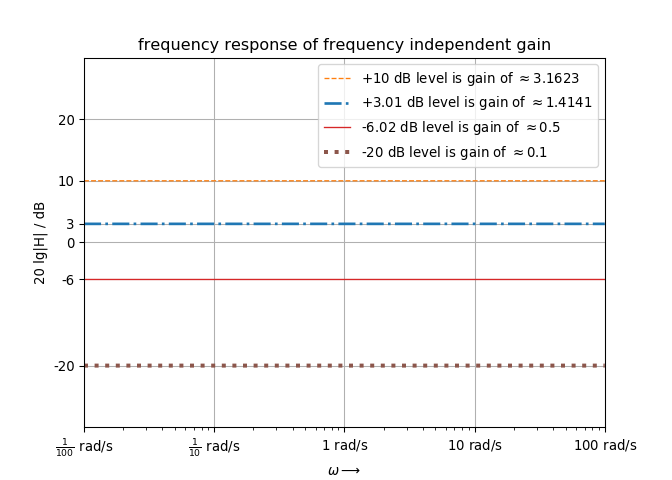
\includegraphics[width=0.5\textwidth]{../laplace_system_analysis/fig_bode_mag_gain}
}
\subfloat[Zeros and poles in origin of $s$-plane, \eq{eq:Hs_sorted_for_Bode_dB_origin}.\label{fig_bode_mag_origin_zeros_poles}]{%
\includegraphics[width=0.5\textwidth]{../laplace_system_analysis/fig_bode_mag_origin_zeros_poles}
}

\subfloat[Single, real zero, \eq{eq:Hs_sorted_for_Bode_dB_zero}.\label{fig_bode_mag_single_zero}]{%
\includegraphics[width=0.5\textwidth]{../laplace_system_analysis/fig_bode_mag_single_zero}
}
\subfloat[Complex conjugate pair of zeros, \eq{eq:Hs_sorted_for_Bode_dB_cczero}.\label{fig_bode_mag_conj_zeros}]{%
\includegraphics[width=0.5\textwidth]{../laplace_system_analysis/fig_bode_mag_conj_zeros}
}

\subfloat[Single, real pole, \eq{eq:Hs_sorted_for_Bode_dB_pole}.\label{fig_bode_mag_single_pole}]{%
\includegraphics[width=0.5\textwidth]{../laplace_system_analysis/fig_bode_mag_single_pole}
}
\subfloat[Complex conjugate pair of poles, \eq{eq:Hs_sorted_for_Bode_dB_ccpole}.\label{fig_bode_mag_conj_poles}]{%
\includegraphics[width=0.5\textwidth]{../laplace_system_analysis/fig_bode_mag_conj_poles}
}
\caption{Level responses of zero / pole prototypes for $s = \sigma + \im \omega$ with $\sigma=0$.
\texttt{bodeplot\_magnitude\_prototypes.ipynb}}
\label{fig:magbodeprototype}
\end{figure}

Recall that for the Laplace variable $s=\sigma + \im\omega$ a chosen  $\sigma=0$
leads to the Fourier transform of $H(s)$, i.e. only harmonic oscillating events
are considered, which we know as steady state.
This is precisely used to discuss the frequency response of an LTI system with
help of the Bode plot.
The level response of the Bode plot evaluates $20 \text{lg} |H(s)\big|_{s=\im \omega}|$.

The \textbf{prototype} systems \eq{eq:Hs_sorted_for_Bode_dB_gain} to
\eq{eq:Hs_sorted_for_Bode_dB_ccpole} exhibit an interesting characteristic,
when being plotted \textbf{over a logarithmic frequency axis}:
In the limiting cases, i.e. for frequencies much larger/smaller than around the pole/zero magnitude, the level response \textbf{can be approximated by straight-line equations}.
These approximations are visualised in Fig. \ref{fig:magbodeprototype}.
For example, for a single, real zero $s_{0,j}$ the prototype level response is $20 \text{lg}  \bigg|\frac{s}{s_{0,j}}-1\bigg|$
according to \eq{eq:Hs_sorted_for_Bode_dB_zero}.
For $|s| \ll |s_{0,j}|$, the value of one is dominating, yielding a line at 0 dB.
For $|s| \gg |s_{0,j}|$, the fraction is prevailing, yielding a line with a rise of 20 dB per decade (i.e. a tenfold increase of frequency).
The asymptotic characteristics changes at $|s| = |s_{0,j}|$.
This is depicted in Fig. \ref{fig_bode_mag_single_zero}.



\clearpage
\subsubsection{Manual Logarithmic Diagram}
It is very helpful when we are able to draw an approximated Bode plot sketch manually.
In order to do this we need to know how the logarithmic frequency axis is designed.
%
In SigSys either the $\log_{10}$ (w.r.t. frequency decade) or $\log_{2}$
(w.r.t. frequency octave) are commonly used.
%
Most important is to realize that each decade (10 times of a reference frequency)
or each octave (2 times of a reference frequency) takes always the same distance
on the x-axis.
%
This is the idea of the log plot.
%
Second, minor grid lines can be set up. For the $\log_{10}$ plot
this is standardized being the numbers from 1 to 10 within one decade.
\begin{center}
\begin{tikzpicture}
\centering
\def \tic {0.05}
\begin{scope}
\draw[->] (-0.5,0) -- (4.5,0) node[right]{$\log_{10} \frac{\omega}{\omega_r}$};
\draw[-] (0,-\tic) -- (0,+\tic) node[below]{$10^{-1}$};
\draw[-] (1,-\tic) -- (1,+\tic) node[below]{$10^{0}$};
\draw[-] (2,-\tic) -- (2,+\tic) node[below]{$10^{1}$};
\draw[-] (3,-\tic) -- (3,+\tic) node[below]{$10^{2}$};
\draw[-] (4,-\tic) -- (4,+\tic) node[below]{$10^{3}$};
\draw[->] (-0.5,0) -- (-0.5,2) node[above]{dB};
\draw[-] (-0.5-\tic,0.5) -- (-0.5+\tic,0.5) node[left]{20};
\draw[-] (-0.5-\tic,1.5) -- (-0.5+\tic,1.5) node[left]{40};
\draw[C0, -, ultra thick] (1,0.5) -- (2,1.5) node[right]{+20dB / decade};
\draw[-.,C7] (0.0,0.5) -- (0.0,1.5);
\draw[-.,C7] (0.30103,0.5) -- (0.30103,1.5);
\draw[-.,C7] (0.47712125,0.5) -- (0.47712125,1.5);
\draw[-.,C7] (0.60205999,0.5) -- (0.60205999,1.5);
\draw[-.,C7] (0.69897,0.5) -- (0.69897,1.5);
\draw[-.,C7] (0.77815125,0.5) -- (0.77815125,1.5);
\draw[-.,C7] (0.84509804,0.5) -- (0.84509804,1.5);
\draw[-.,C7] (0.90308999,0.5) -- (0.90308999,1.5);
\draw[-.,C7] (0.95424251,0.5) -- (0.95424251,1.5);
\draw[-.,C7] (1,0.5) -- (1,1.5);
\end{scope}
%
\begin{scope}[shift={(7,0)}]
\draw[->] (-0.5,0) -- (4.5,0) node[right]{$\log_{2}  \frac{\omega}{\omega_r}$};
\draw[-] (0,-\tic) -- (0,+\tic) node[below]{$2^{-1}$};
\draw[-] (1,-\tic) -- (1,+\tic) node[below]{$2^{0}$};
\draw[-] (2,-\tic) -- (2,+\tic) node[below]{$2^{1}$};
\draw[-] (3,-\tic) -- (3,+\tic) node[below]{$2^{2}$};
\draw[-] (4,-\tic) -- (4,+\tic) node[below]{$2^{3}$};
\draw[->] (-0.5,0) -- (-0.5,2) node[above]{dB};
\draw[-] (-0.5-\tic,0.5) -- (-0.5+\tic,0.5) node[left]{6};
\draw[-] (-0.5-\tic,1.5) -- (-0.5+\tic,1.5) node[left]{12};
\draw[C0, -, ultra thick] (1,0.5) -- (2,1.5) node[right]{$\approx$+6dB / octave};
\draw[-.,C7] (0.0,0.5) -- (0.0,1.5);
\draw[-.,C7] (0.13750352,0.5) -- (0.13750352,1.5);
\draw[-.,C7] (0.26303441,0.5) -- (0.26303441,1.5);
\draw[-.,C7] (0.37851162,0.5) -- (0.37851162,1.5);
\draw[-.,C7] (0.48542683,0.5) -- (0.48542683,1.5);
\draw[-.,C7] (0.5849625,0.5) -- (0.5849625,1.5);
\draw[-.,C7] (0.67807191,0.5) -- (0.67807191,1.5);
\draw[-.,C7] (0.76553475,0.5) -- (0.76553475,1.5);
\draw[-.,C7] (0.84799691,0.5) -- (0.84799691,1.5);
\draw[-.,C7] (0.92599942,0.5) -- (0.92599942,1.5);
\draw[-.,C7] (1,0.5) -- (1,1.5);
\end{scope}
\end{tikzpicture}
\end{center}

%log10 axis spacing:
%[0.         0.30103    0.47712125 0.60205999 0.69897    0.77815125
% 0.84509804 0.90308999 0.95424251 1.        ]
%log2 axis spacing:
%[0.         0.13750352 0.26303441 0.37851162 0.48542683 0.5849625
% 0.67807191 0.76553475 0.84799691 0.92599942 1.        ]


\begin{itemize}
  \item $\log_{10}$:
  (Standardised) grid lines for the first decade in the above example at
  \begin{align}
  10^{-1} \cdot [1,2,3,...,9,10] = [0.1,0.2,0.3,...,0.9,1]
  \end{align}
  to cover frequencies from $\omega=10^{-1} \omega_r$ to $\omega=10^1 \cdot 10^{-1} \omega_r= 10^0 \omega_r$
  can be drawn by the spacing values $\log_{10}[1,2,3,...,9,10]$
  along the relative line from 0 to 1 within this decade.
  \item $\log_{2}$:
  (Potentially meaningful) grid lines for the first octave at
  \begin{align}
  2^{-1} \cdot [1.0, 1.1, 1.2, 1.3,...,2.0]
  \end{align}
  to cover frequencies from $\omega=2^{-1} \omega_r$ to $\omega=2^1 \cdot 2^{-1} \omega_r = 2^0 \omega_r$
  can be drawn by the spacing values $\log_{2}[1,1.1,1.2,...,1.9,2]$
  along the relative line from 0 to 1 within this octave.
\end{itemize}
%
Often $\omega_r = 1$ is chosen.
In SigSys we often deal LTI systems that exhibit slopes of $\pm o \cdot 20$ dB / decade.
20 dB / decade correspond to $20\cdot \log_{10}(2) \approx 6.02$ dB / octave
in a $\log_2$ plot.
Then $\pm$40 dB / decade correspond to $\approx\pm$ 12 dB / octave and so on.





% %\bibliographystyle{IEEEtranSA.bst}
% %\bibliography{literature}
% \clearpage
% \bibliography{literatur}
% \end{document}
  % UE 5, LTI systems in spectral domain, bode plot

\setcounter{section}{5}
%%------------------------------------------------------------------------------
\clearpage
\section{UE 6: Eigenschaften von zeitkontinuierlichen LTI Systemen}

Wir haben mittlerweile den SigSys Werkzeugkoffer gut aufgefüllt um
zeitkontinuierliche Signale und Systeme beschreiben zu können.

In dieser Übung werden wir uns aus diesen Grundzutaten ein paar wichtige
komplexere Werkzeuge zusammenbauen, um Systeme noch besser interpretierbar zu
machen. Das machen wir anhand von drei ganz einfachen Systemen erster Ordnung,
die jeweils einen Pol und eine Nullstelle haben. Ihre Lage bestimmt ganz wesentlich
was das System genau macht. Wenn wir das Wesen hinter diesen neuen Werkzeugen
bzw. Sichtweisen verstanden haben, ist es eine vergleichsweise einfache
Leistung das auf komplexere Systeme (also Systeme mit noch mehr Nullstellen
und Polstellen) zu übertragen.
%
Buzzwords für diese Übung sind
\begin{itemize}
  \item Minimalphasensystem, Maximalphasensystem, Allpass, gemischtphasiges System
  \item Bode Diagramm, Pegeldiagramm
  \item Systementzerrung
  \item Reihenschaltung, Parallelschaltung von Systemen
  \item Phasenfrequenzgang, Gruppenlaufzeit
\end{itemize}
Das sind alles Dinge die in aufbauenden Fächern immer wieder benötigt
werden, z.B. für Regelungstechnik, Mechatronik, Nachrichtentechnik,
Nachrichtenübertragungstechnik und Hochfrequenztechnik.

Diese Übung ist auch wieder sehr dicht und diesmal eigentlich sogar zu viel für
eine Einheit!
Es wäre jedoch schade, nach allem was wir uns wie didaktisch erarbeitet haben,
Inhalte zu kürzen, nur um dem aktuellen verkürzten Semestertakt gerechter
zu werden. Mutmaßlich interessiert es langfristig niemanden, ob wir im SS2020
nur 12 Semesterwochen für SigSys und alle anderen Fächer betrieben haben,
wir brauchen das Handwerk ja so oder so. Das komplette Neudesign der Übungen
war initial genauso angelegt, dass mit dieser Übung 6 der erste große Bogen,
sozusagen die erste Staffel, zu Ende geht und wir die Essenz der SigSys
gesehen haben.
Wir werden in der zweiten Staffel viele bereits bekannte Werkzeuge wiedertreffen.

\newpage
\subsection{Diskussion dreier Systeme 1. Ordnung}
\label{sec:E1E7E53CFF}
\begin{Ziel}
An dieser Stelle wollen wir anhand dreier vergleichsweise einfacher System
nochmal die wichtigsten Berechnungsvorschriften und Kenngrößen von
zeitkontinuierlichen Systemen durchspielen.
Dabei werden wir sehen, dass ein paar Rechnungen schon bei diesen einfachen
Systemen, vergleichsweise komplizierte Formeln erzeugen.
Wir sollten das hier jedoch einmal manuell durchleiden, um die Vorzüge der
Computer Algebra zu schätzen wissen. Systeme höherer Ordnung, also mehr Null-
und Polstellen sind im Grund nicht mehr sinnvoll auf dem Papier zu handhaben.
Daher werden wir in der Praxis diese Systeme aufsplitten in Reihen- oder
Parallelschaltung von Systemen 1. und 2. Ordnung. Es ist daher sehr sinnvoll,
wenn wir uns bei 1./2. Ordnung Systemen 'zu Hause' fühlen.
Hier also zunächst reines Zusammentragen von Ergebnissen, im Grunde stumpfes
Abarbeiten mittlerweile bekannter SigSys-Dinge. Danach werden wir mit diesen
drei Systemen in den nächsten Aufgaben dann noch zu weiteren Erkenntnisse
erlangen.
\end{Ziel}
\textbf{Aufgabe} {\tiny E1E7E53CFF}: Gegeben sind die drei Laplace
Übertragungsfunktionen
\begin{align}
H(s)_\mathrm{max} = \frac{2 s-4}{s+\frac{1}{2}}\qquad
H(s)_\mathrm{min} = \frac{2 s+4}{s+\frac{1}{2}}\qquad
H(s)_\mathrm{all} = \frac{s-2}{s+2}
\end{align}
von kausalen Systemen. Wir berücksichtigen keine Anfangszustände, die Systeme
befinden sich also zum Anregungszeitpunkt in Ruhe.
%
Prüfen Sie die Korrektheit der folgenden Angaben (die Idee ist natürlich,
dass alles stimmt, Typos wären nicht absichtlich):
\begin{itemize}
  \item Impulsantwort (für die Laplace Rücktrafo führt hier die Polynomdivision schneller zum Ziel als Partialbruchzerlegung)
  \begin{align}
  &h(t)_\mathrm{max} = 2\delta(t) - 5\,\e^{-\frac{t}{2}}\,\epsilon(t)\\
  &h(t)_\mathrm{min} = 2\delta(t) + 3\,\e^{-\frac{t}{2}}\,\epsilon(t)\\
  &h(t)_\mathrm{all} = \delta(t) - 4\,\e^{-2\,t}\,\epsilon(t)
  \end{align}
  \item Sprungantwort (Partialbruchzerlegung)
  \begin{align}
  &h_\epsilon(t)_\mathrm{max} = -8 \epsilon(t) + 10 \, \e^{-\frac{t}{2}}\,\epsilon(t)\\
  &h_\epsilon(t)_\mathrm{min} = +8 \epsilon(t) -6 \, \e^{-\frac{t}{2}}\,\epsilon(t)\\
  &h_\epsilon(t)_\mathrm{all} = -\epsilon(t) + 2 \, \e^{-2\,t}\,\epsilon(t)
  \end{align}
  \item Pol-/Nullstellen/Konstante-Diagramme mit Angabe des Konvergenzbereichs

  \begin{tikzpicture}
  \def \axisLength {4}
  \def \tic {0.05}
  \begin{scope}
  \def \sigmaROC {-1/4}
  \def \zero {1}
  \def \convAbsz {\sigmaROC}
  \fill[C2!50] (\convAbsz,-\axisLength/2)--(\convAbsz,\axisLength/2)
  decorate [decoration={snake,segment length=15pt,amplitude=1pt}]
  {(\convAbsz,\axisLength/2)--
  (\axisLength/2,\axisLength/2)--
  (\axisLength/2,-\axisLength/2)--
  (\convAbsz,-\axisLength/2)};
  \draw[->] (-\axisLength/2,0)--(\axisLength/2,0) node[right]{\small$\Re\{s\}$};
  \draw[->] (0,-\axisLength/2)--(0,\axisLength/2) node[above]{\small$\Im\{s\}$};
  \draw[-, C3] (0,+\axisLength/2+1/2)--(0,-\axisLength/2-1/2) node[below]{\small$\textcolor{C3}{H(\im\omega)_\mathrm{max}}$};
  \draw[C0, ultra thick] (\sigmaROC,0) node{\Huge $\times$};
  \draw[C0, ultra thick] (\zero,0) node{\Huge $\circ$};
  \draw (\sigmaROC,\tic)--(\sigmaROC,-\tic) node[below]{$-\frac{1}{2}$};
  \draw (\zero,\tic)--(\zero,-\tic) node[below]{$2$};
  \draw (1.25,+2.25) node[C2!75]{ROC};
  \draw (1.25,1.75) node[]{$H_0=2$};
  \draw (3,1) node[]{\Large$=$};
  \end{scope}
  %
  %
  %
  \begin{scope}[shift={(5,0)}]
  \def \sigmaROC {-1/4}
  \def \zero {-1}
  \def \convAbsz {\sigmaROC}
  \fill[C2!50] (\convAbsz,-\axisLength/2)--(\convAbsz,\axisLength/2)
  decorate [decoration={snake,segment length=15pt,amplitude=1pt}]
  {(\convAbsz,\axisLength/2)--
  (\axisLength/2,\axisLength/2)--
  (\axisLength/2,-\axisLength/2)--
  (\convAbsz,-\axisLength/2)};
  \draw[->] (-\axisLength/2,0)--(\axisLength/2,0) node[right]{\small$\Re\{s\}$};
  \draw[->] (0,-\axisLength/2)--(0,\axisLength/2) node[above]{\small$\Im\{s\}$};
  \draw[-, C3] (0,+\axisLength/2+1/2)--(0,-\axisLength/2-1/2) node[below]{\small$\textcolor{C3}{H(\im\omega)_\mathrm{min}}$};
  \draw[C0, ultra thick] (\sigmaROC,0) node{\Huge $\times$};
  \draw[C0, ultra thick] (\zero,0) node{\Huge $\circ$};
  \draw (\sigmaROC,\tic)--(\sigmaROC,-\tic) node[below]{$-\frac{1}{2}$};
  \draw (\zero,\tic)--(\zero,-\tic) node[below]{$-2$};
  \draw (1.25,+2.25) node[C2!75]{ROC};
  \draw (1.25,1.75) node[]{$H_0=2$};
  \draw (3,1) node[]{\Large$\cdot$};
  \end{scope}
  %
  %
  %
  \begin{scope}[shift={(10,0)}]
  \def \sigmaROC {-1}
  \def \zero {+1}
  \def \convAbsz {\sigmaROC}
  \fill[C2!50] (\convAbsz,-\axisLength/2)--(\convAbsz,\axisLength/2)
  decorate [decoration={snake,segment length=15pt,amplitude=1pt}]
  {(\convAbsz,\axisLength/2)--
  (\axisLength/2,\axisLength/2)--
  (\axisLength/2,-\axisLength/2)--
  (\convAbsz,-\axisLength/2)};
  \draw[->] (-\axisLength/2,0)--(\axisLength/2,0) node[right]{\small$\Re\{s\}$};
  \draw[->] (0,-\axisLength/2)--(0,\axisLength/2) node[above]{\small$\Im\{s\}$};
  \draw[-, C3] (0,+\axisLength/2+1/2)--(0,-\axisLength/2-1/2) node[below]{\small$\textcolor{C3}{H(\im\omega)_\mathrm{all}}$};
  \draw[C0, ultra thick] (\sigmaROC,0) node{\Huge $\times$};
  \draw[C0, ultra thick] (\zero,0) node{\Huge $\circ$};
  \draw (\sigmaROC,\tic)--(\sigmaROC,-\tic) node[below]{$-2$};
  \draw (\zero,\tic)--(\zero,-\tic) node[below]{$+2$};
  \draw (1.25,+2.25) node[C2!75]{ROC};
  \draw (1.25,1.75) node[]{$H_0=1$};
  \end{scope}
  \end{tikzpicture}

\item Bode Diagramm Approximation für Pegel über Kreisfrequenz

\begin{tikzpicture}
\begin{scope}
\def \tic {0.05}
\draw[->] (-0.5,0) -- (4.5,0) node[right]{$\log_{2}  \omega$};
\draw[-] (0,-\tic) -- (0,+\tic) node[below]{$2^{-2}$};
\draw[-] (1,-\tic) -- (1,+\tic) node[below]{$2^{-1}$};
\draw[-] (2,-\tic) -- (2,+\tic) node[below]{$2^{0}$};
\draw[-] (3,-\tic) -- (3,+\tic) node[below]{$2^{1}$};
\draw[-] (4,-\tic) -- (4,+\tic) node[below]{$2^{2}$};
\draw[->] (-0.5,0) -- (-0.5,3.5) node[above]{dB};
\draw[-] (-0.5-\tic,1) -- (-0.5+\tic,1) node[left]{$6$};
\draw[-] (-0.5-\tic,2) -- (-0.5+\tic,2) node[left]{$12$};
\draw[-] (-0.5-\tic,3) -- (-0.5+\tic,3) node[left]{$18$};
\draw[C0, -, ultra thick] (-0.5,3) -- (1,3) -- (3,1) -- (4,1);
\draw (1,1) node[]{$20\mathrm{lg}|H(\im\omega)_\mathrm{max}|$};
\draw (1,0.5) node[]{$20\mathrm{lg}|H(\im\omega)_\mathrm{min}|$};
\end{scope}
%
%
%
\begin{scope}[shift={(7,0)}]
\def \tic {0.05}
\draw[->] (-0.5,0) -- (4.5,0) node[right]{$\log_{2}  \omega$};
\draw[-] (0,-\tic) -- (0,+\tic) node[below]{$2^{-2}$};
\draw[-] (1,-\tic) -- (1,+\tic) node[below]{$2^{-1}$};
\draw[-] (2,-\tic) -- (2,+\tic) node[below]{$2^{0}$};
\draw[-] (3,-\tic) -- (3,+\tic) node[below]{$2^{1}$};
\draw[-] (4,-\tic) -- (4,+\tic) node[below]{$2^{2}$};
\draw[->] (-0.5,0) -- (-0.5,3.5) node[above]{dB};
\draw[-] (-0.5-\tic,1) -- (-0.5+\tic,1) node[left]{$-6$};
\draw[-] (-0.5-\tic,2) -- (-0.5+\tic,2) node[left]{$0$};
\draw[-] (-0.5-\tic,3) -- (-0.5+\tic,3) node[left]{$+6$};
\draw[C0, -, ultra thick] (-0.5,2) -- (4,2);
\draw (1,1) node[]{$20\mathrm{lg}|H(\im\omega)_\mathrm{all}|$};
\end{scope}
\end{tikzpicture}

\item Analytische Kurvendiskussion für $H(s)_\mathrm{max}$
\begin{align}
%&H(s)_\mathrm{max} = 2\cdot\frac{s-2}{s+\frac{1}{2}}\\
&H(\im\omega)_\mathrm{max} = 2\cdot\frac{\im\omega-2}{\im\omega+\frac{1}{2}}=
\frac{8\,\omega^2 - 8}{1+4\,\omega^2}+
\im\cdot \frac{20\omega}{1+4\,\omega^2}\\
&20 \log_{10}|H(\im\omega)_\mathrm{max}| =
10 \log_{10} \left(\frac{(8 \omega^2 -8)^2 + 400 \omega^2}{(1+4\omega^2)^2}\right)\text{in dB}\\
&\angle H(\im\omega)_\mathrm{max} =
\mathrm{atan}\left(\frac{20}{8\omega-\frac{8}{\omega}}\right)\text{in rad}\\
&-\frac{\fsd}{\fsd \omega} \angle H(\im\omega)_\mathrm{max}=
\frac{10(\omega^2+1)}{4\omega^4+17\omega^2+4}\text{in s}\\
&|H(\im[\omega\to 0])_\mathrm{max}| = 8, \angle H(\im[\omega\to 0])_\mathrm{max} = \pi\\
&|H(\im[\omega\to\infty])_\mathrm{max}| = 2, \angle H(\im[\omega\to\infty])_\mathrm{max} = 0\\
&|H(\im[\omega\to 1])_\mathrm{max}| = 4, \angle H(\im[\omega\to 1])_\mathrm{max} = \frac{\pi}{2}
\end{align}

\item Analytische Kurvendiskussion für $H(s)_\mathrm{min}$
\begin{align}
%&H(s)_\mathrm{min} = 2\cdot\frac{s+2}{s+\frac{1}{2}}\\
&H(\im\omega)_\mathrm{min} = 2\cdot\frac{\im\omega+2}{\im\omega+\frac{1}{2}}=
\frac{8\,\omega^2 + 8}{1+4\,\omega^2}-
\im\cdot \frac{12\omega}{1+4\,\omega^2}
\\
&20 \log_{10}|H(\im\omega)_\mathrm{min}| =
10 \log_{10} \left(\frac{(8\,\omega^2 + 8)^2 + 144\omega^2}{(1+4\,\omega^2)^2}\right)\text{in dB}\\
&\angle H(\im\omega)_\mathrm{min} =
\mathrm{atan}\left(\frac{-12}{8\omega+\frac{8}{\omega}}\right)\text{in rad}\\
&-\frac{\fsd}{\fsd \omega} \angle H(\im\omega)_\mathrm{min}=
\frac{-6(\omega^2-1)}{4\omega^4+17\omega^2+4}\text{in s}\\
&|H(\im[\omega\to 0])_\mathrm{min}| = 8 = , \angle H(\im[\omega\to 0])_\mathrm{min} = 0\\
&|H(\im[\omega\to\infty])_\mathrm{min}| = 2 = , \angle H(\im[\omega\to\infty])_\mathrm{min} = 0\\
&|H(\im[\omega\to 1])_\mathrm{min}| = 4, \angle H(\im[\omega\to 1])_\mathrm{min} = -\mathrm{atan}(\nicefrac{3}{4}) \approx -36.87^\circ
\end{align}

\item Analytische Kurvendiskussion für $H(s)_\mathrm{all}$
\begin{align}
%&H(s)_\mathrm{all} = \frac{s-2}{s+2}\\
&H(\im\omega)_\mathrm{all} = \frac{\im\omega-2}{\im\omega+2}=
\frac{\omega^2-4}{\omega^2+4}+
\im\cdot\frac{4\omega}{\omega^2+4}\\
&20 \log_{10}|H(\im\omega)_\mathrm{all}| =
10 \log_{10} \left(\frac{(\omega^2-4)^2+16\omega^2}{(\omega^2+4)^2}\right)\text{in dB}\\
&\angle H(\im\omega)_\mathrm{all} =
\mathrm{atan}\left(\frac{4}{\omega-\frac{4}{\omega}}\right)\text{in rad}\\
&-\frac{\fsd}{\fsd \omega} \angle H(\im\omega)_\mathrm{all}=
\frac{4}{\omega^2+4}\text{in s}\\
&|H(\im[\omega\to 0])_\mathrm{all}| = 1, \angle H(\im[\omega\to 0])_\mathrm{all} = \pi\\
&|H(\im[\omega\to\infty])_\mathrm{all}| = 1, \angle H(\im[\omega\to\infty])_\mathrm{all} = 0\\
&|H(\im[\omega\to 1])_\mathrm{all}| = 1, \angle H(\im[\omega\to 1])_\mathrm{all} = \pi - \mathrm{atan}(\nicefrac{4}{3}) \approx +126.87^\circ
\end{align}

\item die in \fig{fig:MaxMinPhaseAllpass_numpy_E1E7E53CFF} gezeichneten exakten
Bode Diagramme. Wir sollten in der Lage sein, mit einem Computer Algebra Programm
unserer Wahl diese Grafiken selber erzeugen und mit den Ergebnissen
aus den Kurvendiskussion auf Plausibilität prüfen zu können.

\end{itemize}

\noindent \textbf{Computer Algebra Hilfsmittel}

\noindent Unter

\url{https://github.com/spatialaudio/signals-and-systems-exercises}

\noindent im Ordner

\texttt{system\_properties\_ct}

\noindent stehen die beiden Jupyter Notebooks

\texttt{MaxMinPhaseAllpass\_numpy\_E1E7E53CFF.ipynb}

\texttt{MaxMinPhaseAllpass\_sympy\_E1E7E53CFF.ipynb}

\noindent zur Verfügung, mit denen Bode Diagramme der betrachteten Beispiele visualisiert
werden können. Dies eignet sich auch für weitere Experimente.
Sehr bequem kann das Bode Diagramm auch bei Wolfram Alpha, z.B. mit

\url{https://www.wolframalpha.com/input/?i=bode+plot+2*%28s-2%29%2F%28s%2B1%2F2%29}

\noindent  berechnet und dargestellt werden. Nützlich ist dort auch die Möglichkeit
der Partialbruchzerlegung

\url{https://www.wolframalpha.com/input/?i=partial+fraction+expansion+2*%28s-2%29%2F%28s%2B1%2F2%29}

\noindent Der Matlab Code in \texttt{laplace\_system\_analysis/bode\_diagramme.m}
könnte auch nützlich sein.

\clearpage
\begin{figure*}[h]
\centering
\begin{subfigure}{0.7\textwidth}
\includegraphics[width=\textwidth]{../system_properties_ct/MaxMinPhaseAllpass_numpy_E1E7E53CFF_maxphase.pdf}
\caption{Bode Diagramm für System $H(s)_\mathrm{max}$}
\label{fig:MaxMinPhaseAllpass_numpy_E1E7E53CFF_maxphase}
\end{subfigure}
\begin{subfigure}{0.7\textwidth}
\includegraphics[width=\textwidth]{../system_properties_ct/MaxMinPhaseAllpass_numpy_E1E7E53CFF_minphase.pdf}
\caption{Bode Diagramm für System $H(s)_\mathrm{min}$}
\label{fig:MaxMinPhaseAllpass_numpy_E1E7E53CFF_minphase}
\end{subfigure}
\begin{subfigure}{0.7\textwidth}
\includegraphics[width=\textwidth]{../system_properties_ct/MaxMinPhaseAllpass_numpy_E1E7E53CFF_allpass.pdf}
\caption{Bode Diagramm für System $H(s)_\mathrm{all}$}
\label{fig:MaxMinPhaseAllpass_numpy_E1E7E53CFF_allpass}
\end{subfigure}
\caption{Systeme aus Aufgabe \ref{sec:E1E7E53CFF}. \texttt{MaxMinPhaseAllpass\_numpy\_E1E7E53CFF.ipynb}}
\label{fig:MaxMinPhaseAllpass_numpy_E1E7E53CFF}
\end{figure*}
\clearpage
%\begin{Werkzeug}
%SigSys...
%\end{Werkzeug}
%\begin{Ansatz}
%\end{Ansatz}
%\begin{ExCalc}
%\end{ExCalc}
%\begin{Loesung}
%\end{Loesung}


% Impulsantworten mittels Polynomdivision, einfache Parallelschaltungen:
% \begin{align}
% H(s)_\mathrm{max} = H(s)_\mathrm{Max Phase} = 2 - \frac{5}{s+\nicefrac{1}{2}}
% &\quad\Laplace\quad h(t)_\mathrm{max} = 2\delta(t) - 5\,\e^{-\frac{t}{2}}\,\epsilon(t)\\
% H(s)_\mathrm{min}  = H(s)_\mathrm{Min Phase} = 2 + \frac{3}{s+\nicefrac{1}{2}}
% &\quad\Laplace\quad h(t)_\mathrm{min} = 2\delta(t) + 3\,\e^{-\frac{t}{2}}\,\epsilon(t)\\
% H(s)_\mathrm{all}  = H(s)_\mathrm{Allpass} =  1 - \frac{4}{s+2}
% &\quad\Laplace\quad h(t)_\mathrm{all} = \delta(t) - 4\,\e^{-2\,t}\,\epsilon(t)
% \end{align}
%
% Sprungantworten mit PZB:
% \begin{align}
% H(s)_\mathrm{max} \cdot \frac{1}{s} = 2\cdot\frac{s-2}{s+\frac{1}{2}} \cdot \frac{1}{s}
% &\quad\Laplace h_\epsilon(t)_\mathrm{max} = -8 \epsilon(t) + 10 \, \e^{-\frac{t}{2}}\,\epsilon(t)\\
% H(s)_\mathrm{min} \cdot \frac{1}{s} = 2\cdot\frac{s+2}{s+\frac{1}{2}} \cdot \frac{1}{s}
% &\quad\Laplace h_\epsilon(t)_\mathrm{min} = +8 \epsilon(t) -6 \, \e^{-\frac{t}{2}}\,\epsilon(t)\\
% H(s)_\mathrm{all} \cdot \frac{1}{s} = \frac{s-2}{s+2} \cdot \frac{1}{s}
% &\quad\Laplace h_\epsilon(t)_\mathrm{all} = -\epsilon(t) + 2 \, \e^{-2\,t}\,\epsilon(t)
% \end{align}






































\newpage
\subsection{Zerlegung in Reihenschaltung aus Minimalphasensystem und Allpass}
\label{sec:68CD3A7F90}
\begin{Ziel}
Wir wollen uns anhand eines
einfachen Beispiels die Begriffe maximalphasig, minimalphasig und Allpass erarbeiten.
Jedes stabile, kausale System kann zerlegt werden in eine Reihenschaltung aus
Minimalphasensystem und Allpass.
\end{Ziel}
\textbf{Aufgabe} {\tiny 68CD3A7F90}: Gegeben ist die Laplace
Übertragungsfunktion
\begin{align}
H(s)_\mathrm{max} = \frac{2 s-4}{s+\frac{1}{2}}\qquad
\end{align}
eines kausalen Systems. Wir berücksichtigen keine Anfangszustände.
Zerlegen Sie dieses System in seinen Allpass- und minimalphasigen Anteil.





\begin{Werkzeug}
\begin{itemize}
  \item Reihenschaltung von $H_1(s)$ und $H_2(s)$ ergibt Gesamtübertragungsfunktion
  \begin{align}
    H(s) = H_1(s) \cdot H_2(s)
  \end{align}
  und wir erinnern uns, dass $H_1(s)\cdot H_2(s) \,\Laplace\, h_1(t)\ast h_2(t)$
  und $h(t) = h(t)\ast \delta(t)$
  \item \textbf{Minimalphasensystem}: Nullstellen nur in der linken $s$-Ebene. Da prinzipiell
  Stabilität gefordert wurde, gilt also die Regel: alle Pole und alle Nullstellen
  befinden sich in der linken $s$-Ebene.
  \item \textbf{Maximalphasensystem}: Nullstellen nur in der rechten $s$-Ebene. Da prinzipiell
  Stabilität gefordert wurde, gilt also die Regel: alle Pole in der linken
  $s$-Ebene und alle Nullstellen in der rechten $s$-Ebene.
  \item \textbf{Allpasssystem}: nur spiegelbildliche Pol-Nullstellenpaare bzgl.
  der $\im\omega$-Achse. Da prinzipiell Stabilität gefordert wurde, gilt also
  die Regel: alle Pole in der linken $s$-Ebene und zu jedem Pol gehört
  eine an $\im\omega$ gespiegelte Nullstelle in der rechten $s$-Ebene.
  Betrag über $\omega$ ist konstant, Konvention: Betrag ist 1.
\end{itemize}


\end{Werkzeug}
\begin{Ansatz}
Zu lösen entweder analytisch, also mit der Übertragungsfunktion als Formel
oder grafisch anhand von Pol-Nullstellen Diagrammen.
\end{Ansatz}

\begin{ExCalc}
\textbf{Analytisch}:
Wir können $H(s)_\mathrm{max} $ zunächst in Pol-, Nullstellen und frequenzunabhängige
Konstante Darstellung bringen
\begin{align}
H(s)_\mathrm{max} = 2\cdot\frac{s-2}{s+\frac{1}{2}}
\end{align}
und sehen schnell, dass die einzige Nullstelle in der rechten $s$-Ebene liegt.
Für ein Minimalphasensystem brauchen wir aber eine Nullstelle, die bzgl. der Auswertung
Betragsfrequenzgangs entlang der $\im\omega$-Achse das selbe macht, allerdings
eben wie gefordert in der linken $s$-Ebene.
Das ist die Nullstelle exakt an der $\im\omega$-Achse gespiegelt.
Wir können uns das klar machen, wenn wir uns nochmal anschauen, wie das Bode
Diagramm approximiert gezeichnet wird (siehe UE 5):
Wir benutzen die Beträge $|s_{0,\cdot}|$ um die Knickpunkte für
die stückweisen Geraden zu bestimmen.
Der Vorzeichenwechsel des Realteils einer Nullstelle entspricht genau der
geforderten Spiegelung an $\im\omega$, der Betrag der komplexen Zahl ändert
sich dadurch aber nicht. Das Pegeldiagramm bleibt daher gleich. Vorsicht: der
Phasenfrequenzgang ändert sich sehr wohl, das ist der Gag an der Sache. Wir kommen
später in der Übung darauf zurück.

Wir erweitern,
nun die Übertragungsfunktion um den Bruch
\begin{align}
H(s)_\mathrm{max} = 2\cdot\frac{s-2}{s+\frac{1}{2}} \cdot \frac{s+2}{s+2},
\end{align}
also mit der gespiegelten Nullstelle, die wir aber mit einer Polstelle
an der gleichen Stelle gleich wieder 'entschärfen', sich aufhebende Pole und Nullstellen
ändern ja nichts an der Übertragungsfunktion und in Folge auch nicht am Betrags-
und Phasenfrequenzgang.
Der eher langweilige Teil ist nun, die richtigen Anteile in dem Bruchausdruck
jeweils dem Allpass und dem Minimalphasensystem zuzuordnen.
Dazu müssen die obigen Regeln befolgt werden.

Erfahrungsgemäß ist es einfacher mit dem Minimalphasensystem zu beginnen, also
alle Pole und alle Nullstellen zu separieren, die in der linken $s$-Ebene sind.
Das ist also
\begin{align}
H(s)_\mathrm{min}  = H(s)_\mathrm{Min Phase} = 2\cdot\frac{s+2}{s+\frac{1}{2}},
\end{align}
wo wir auch noch den Verstärkungsfaktor mitnehmen, weil nach unserer Konvention
der Allpass immer Betrag 1 hat.
Die übrig gebliebenen Terme
\begin{align}
H(s)_\mathrm{all}  = H(s)_\mathrm{Allpass} =  \frac{s-2}{s+2}
\end{align}
ergeben dann, wenn wir alles richtig gemacht haben, den Allpass.
Nochmal zur Kontrolle:
\begin{align}
H(s) =
\underbrace{\left(2\cdot\frac{s-2}{s+\frac{1}{2}}\right)}_{\mathrm{max phase}} =
\underbrace{\left(2\cdot\frac{s+2}{s+\frac{1}{2}}\right)}_{\mathrm{min phase}}
\cdot \underbrace{\frac{s-2}{s+2}}_{\mathrm{Allpass}}
\end{align}
Das erscheint hier noch sehr übersichtlich, bei Systemen höherer Ordnung
müssen wir dann schon genauer hinschauen und alles sorgfältig aufschreiben.
%
Wir kennen diese Systeme natürlich schon, es sind jene aus Aufgabe \ref{sec:E1E7E53CFF}.

\textbf{Hinweis}: Wir haben es hier mit einem Spezialfall der Zerlegung zu tun,
weil unser Ausgangssystem die zusätzliche Eigenschaft eines Maximalphasensystems
hat. Das ist didaktisch sinnvoll gewählt.
Wir können aber jedes beliebige System (oft gemischtphasig bezeichnet) einer
Zerlegung unterziehen, solange es nur stabil ist. Wenn wir also praktischerweise
kausale Systeme einfordern, haben wir es dann mit Polen nur in der linken $s$-Ebene
und Nullstellen beliebig verteilt (reell oder konjugiert-komplex)
in der $s$-Ebene zu tun.
Die Nullstellen die dann schon in der linken $s$-Ebene sind, haben
dann für sich schon minimalphasige Eigenschaft, wir müssen uns dann nur noch
um die in der rechten $s$-Ebene kümmern.

In einem anderen Spezialfall
könnten wir ein bereits minimalphasiges System in Minimalphasensystem und
Allpasssystem zerlegen wollen, das ist ja nicht verboten.
Quizfrage: Wie lautet die Übertragungsfunktion und die Impulsantwort des dann
resultierenden Allpasses.

\end{ExCalc}

%Zerlegung in ein System mit minimaler Phase und ein System mit Allpasscharakteristik
%\begin{align}
%H(s)_\mathrm{max} = H(s)_\mathrm{Max Phase} =& 2\cdot\frac{s-2}{s+\frac{1}{2}}\\
%H(s)_\mathrm{min}  = H(s)_\mathrm{Min Phase} =& 2\cdot\frac{s+2}{s+\frac{1}{2}}\\
%H(s)_\mathrm{all}  = H(s)_\mathrm{Allpass} =&  \frac{s-2}{s+2}
%\end{align}

\begin{tikzpicture}
\def \axisLength {4}
\def \tic {0.05}
\begin{scope}
\def \sigmaROC {-1/4}
\def \zero {1}
\def \convAbsz {\sigmaROC}
\fill[C2!50] (\convAbsz,-\axisLength/2)--(\convAbsz,\axisLength/2)
decorate [decoration={snake,segment length=15pt,amplitude=1pt}]
{(\convAbsz,\axisLength/2)--
(\axisLength/2,\axisLength/2)--
(\axisLength/2,-\axisLength/2)--
(\convAbsz,-\axisLength/2)};
\draw[->] (-\axisLength/4,0)--(\axisLength/2,0) node[right]{\small$\Re\{s\}$};
\draw[->] (0,-\axisLength/2)--(0,\axisLength/2) node[above]{\small$\Im\{s\}$};
\draw[-, C3] (0,+\axisLength/2+1/2)--(0,-\axisLength/2-1/2) node[below]{\small$\textcolor{C3}{H(\im\omega)_\mathrm{max}}$};
\draw[C0, ultra thick] (\sigmaROC,0) node{\Huge $\times$};
\draw[C0, ultra thick] (\zero,0) node{\Huge $\circ$};
\draw (\sigmaROC,\tic)--(\sigmaROC,-\tic) node[below]{$-\frac{1}{2}$};
\draw (\zero,\tic)--(\zero,-\tic) node[below]{$2$};
\draw (1.25,+2.25) node[C2!75]{ROC};
\draw (1.25,1.75) node[]{$H_0=2$};
\draw (3,1) node[]{\Large$=$};
\end{scope}
%
%
%
\begin{scope}[shift={(4.5,0)}]
\def \sigmaROC {-1/4}
\def \zero {1}
\def \convAbsz {\sigmaROC}
\fill[C2!50] (\convAbsz,-\axisLength/2)--(\convAbsz,\axisLength/2)
decorate [decoration={snake,segment length=15pt,amplitude=1pt}]
{(\convAbsz,\axisLength/2)--
(\axisLength/2,\axisLength/2)--
(\axisLength/2,-\axisLength/2)--
(\convAbsz,-\axisLength/2)};
\draw[->] (-\axisLength/4,0)--(\axisLength/2,0) node[right]{\small$\Re\{s\}$};
\draw[->] (0,-\axisLength/2)--(0,\axisLength/2) node[above]{\small$\Im\{s\}$};
\draw[-, C3] (0,+\axisLength/2+1/2)--(0,-\axisLength/2-1/2) node[below]{\small$\textcolor{C3}{H(\im\omega)_\mathrm{max}}$};
\draw[C0, ultra thick] (\sigmaROC,0) node{\Huge $\times$};
\draw[C3, ultra thick] (\zero,0) node{\Huge $\circ$};
\draw[C0, ultra thick] (-\zero,0) node{\Huge $\circ$};
\draw[C3, ultra thick] (-\zero,0) node{\Huge $\times$};
\draw (\sigmaROC,\tic)--(\sigmaROC,-\tic) node[below]{$-\frac{1}{2}$};
\draw (\zero,\tic)--(\zero,-\tic) node[below]{$2$};
\draw (-\zero,\tic)--(-\zero,-\tic) node[below]{$-2$};
\draw (1.25,+2.25) node[C2!75]{ROC};
\draw (1.25,1.75) node[]{$H_0=2$};
\draw (3,1) node[]{\Large$=$};
\end{scope}
%
%
%
\begin{scope}[shift={(9,0)}]
\def \sigmaROC {-1/4}
\def \zero {-1}
\def \convAbsz {\sigmaROC}
\fill[C2!50] (\convAbsz,-\axisLength/2)--(\convAbsz,\axisLength/2)
decorate [decoration={snake,segment length=15pt,amplitude=1pt}]
{(\convAbsz,\axisLength/2)--
(\axisLength/2,\axisLength/2)--
(\axisLength/2,-\axisLength/2)--
(\convAbsz,-\axisLength/2)};
\draw[->] (-\axisLength/4,0)--(\axisLength/2,0) node[right]{\small$\Re\{s\}$};
\draw[->] (0,-\axisLength/2)--(0,\axisLength/2) node[above]{\small$\Im\{s\}$};
\draw[-, C3] (0,+\axisLength/2+1/2)--(0,-\axisLength/2-1/2) node[below]{\small$\textcolor{C3}{H(\im\omega)_\mathrm{min}}$};
\draw[C0, ultra thick] (\sigmaROC,0) node{\Huge $\times$};
\draw[C0, ultra thick] (\zero,0) node{\Huge $\circ$};
\draw (\sigmaROC,\tic)--(\sigmaROC,-\tic) node[below]{$-\frac{1}{2}$};
\draw (\zero,\tic)--(\zero,-\tic) node[below]{$-2$};
\draw (1.25,+2.25) node[C2!75]{ROC};
\draw (1.25,1.75) node[]{$H_0=2$};
\draw (3,1) node[]{\Large$\cdot$};
\end{scope}
%
%
%
\begin{scope}[shift={(13.5,0)}]
\def \sigmaROC {-1}
\def \zero {+1}
\def \convAbsz {\sigmaROC}
\fill[C2!50] (\convAbsz,-\axisLength/2)--(\convAbsz,\axisLength/2)
decorate [decoration={snake,segment length=15pt,amplitude=1pt}]
{(\convAbsz,\axisLength/2)--
(\axisLength/2,\axisLength/2)--
(\axisLength/2,-\axisLength/2)--
(\convAbsz,-\axisLength/2)};
\draw[->] (-\axisLength/4,0)--(\axisLength/2,0) node[right]{\small$\Re\{s\}$};
\draw[->] (0,-\axisLength/2)--(0,\axisLength/2) node[above]{\small$\Im\{s\}$};
\draw[-, C3] (0,+\axisLength/2+1/2)--(0,-\axisLength/2-1/2) node[below]{\small$\textcolor{C3}{H(\im\omega)_\mathrm{all}}$};
\draw[C3, ultra thick] (\sigmaROC,0) node{\Huge $\times$};
\draw[C3, ultra thick] (\zero,0) node{\Huge $\circ$};
\draw (\sigmaROC,\tic)--(\sigmaROC,-\tic) node[below]{$-2$};
\draw (\zero,\tic)--(\zero,-\tic) node[below]{$+2$};
\draw (1.25,+2.25) node[C2!75]{ROC};
\draw (1.25,1.75) node[]{$H_0=1$};
\end{scope}
\end{tikzpicture}

\begin{ExCalc}
\textbf{Grafische Lösung}: Dieser Weg ist in der Klausur beliebt.
Bei einem System höherer Ordnung herrscht ein wenig mehr Übersichtlichkeit,
wir müssen nur darauf achten den frequenzunabhängigen Term $H_0$ nicht zu vergessen.

Die Lösung ist in der Grafik oben veranschaulicht. Zunächst ganz links unser
Ausgangspunkt, das zu zerlegende System, hier maximalphasig, d.h.
alle Nullstellen (hier eine) sind in der rechten $s$-Ebene.
Durch den gegebenen Konvergenzbereich wissen wir, dass das System kausal ist.
Da alle Pole (hier einer) in der linken $s$-Ebene liegen, ist das System
stabil.

Für das nächste Bild müssen wir nun alle rechtsseitigen Nullstellen
suchen und die gespiegelten linksseitigen Nullstellen hinzufügen und unmittelbar
mit Polstellen kompensieren.
Im Beispiel ist das bei $s=-2$ eine Nullstelle und eine Polstelle,
die sich in ihrer Wirkung aufheben, daher ist das immer noch das gleiche
Systemverhalten wie ganz links.

Danach erfolgt die Zerlegung, die grafisch u.U. anschaulicher gelingt, als in Formeln.
Diesmal ist es günstiger mit dem Allpass anzufangen.
Wir suchen dafür alle rechtsseitigen Nullstellen (die sehen wir sehr schnell, weil
in der rechten $s$-Ebene bei staibilen Systemen sonst nix weiter sein sollte)
und die dazu passenden gespiegelten Polstellen, also im Beispiel bei $s=\pm 2$.
Dies ist im Bild ganz rechts zu sehen.

Die verbleibenden Pole und Nullstellen müssen in der linken $s$-Ebene liegen und
bilden das Minimalphasensystem, dieses bekommt dann noch den Faktor $H_0$ des
ursprünglichen Systems zugewiesen, also hier $H_0=2$, im dritten Bild von links.

Zur Kontrolle können wir die Reihenschaltung nochmal in Gedanken durchführen:
beide Pol-Nullstellendiagramme auf transparentem Papier übereinandergelegt,
muss das ursprüngliche Pol-Nullstellendiagramm ergeben.

\end{ExCalc}


\begin{Loesung}
\begin{align}
H(s) =
\underbrace{\left(2\cdot\frac{s-2}{s+\frac{1}{2}}\right)}_{\mathrm{max phase}} =
\underbrace{\left(2\cdot\frac{s+2}{s+\frac{1}{2}}\right)}_{\mathrm{min phase}}
\cdot \underbrace{\frac{s-2}{s+2}}_{\mathrm{Allpass}}
\end{align}

Quizfrage: Der Allpass hat ja frequenzunabhängigen Betragsfrequenzgang von 1,
können wir uns das anhand der Pol- und Nullstellenlage erklären?
\end{Loesung}






\newpage
\subsection{Inversion von Übertragungsfunktionen}
\label{sec:4926427BA9}
\begin{Ziel}
Oft ist die Entzerrung eines Systems $H(s)$ mit einem in Reihe
geschalteten Korrektursystem $H_i(s)$
erwünscht, so dass ideal das Gesamtsystemverhalten $H_r(s)$
\begin{align}
\label{eq:4926427BA9_EQing}
  H_r(s) = H(s)\cdot H_i(s) = 1 \Laplace h_t(t)=\delta(t)
\end{align}
resultiert.
Eine nicht ganz so strenge Version wäre
\begin{align}
  H_r(s) = H(s)\cdot H_i(s) = \e^{-\im\omega\tau} \Laplace h_r(t)=\delta(t-\tau)
\end{align}
mit zugelassener Verzögerung $\tau>0$, d.h. das Gesamtsystem hat diracförmige
Impulsantwort, aber mit Verzögerung. Warum streben wir das an? Erinnern wir uns:
Für $y(t) = h_r(t)\ast x(t)$ wird $x(t-\tau) = \delta(t-\tau)\ast x(t)$, d.h.
das Signal erfährt außer der Verzögerung keine weitere Manipulation bei der Faltung
mit der Impulsantwort des Gesamtsystems, also des hier perfekt entzerrten Systems.
In der Nachrichtenübertragung spielt das eine wichtige Rolle, weil wir
gewillt sind unsere mühevoll erzeugten Sendesignale nicht zu stark
bei der Übertragung (was durch Systeme modelliert wird) zu verformen.
Wir betrachten Übertragungskanalentzerrung hier als Einstieg extrem vereinfacht mit
\eq{eq:4926427BA9_EQing} und es stellt sich die Frage, wann $H_i(s)$ eigentlich
existiert oder in SigSys-Sprech unter welchen Bedingungen $H_i(s)$
ein stabiles, kausales und deshalb praktikables System ist.
\end{Ziel}
\textbf{Aufgabe} {\tiny 4926427BA9}: Gegeben sind die Laplace
Übertragungsfunktionen
\begin{align}
H(s)_\mathrm{max} = \frac{2 s-4}{s+\frac{1}{2}}\qquad
H(s)_\mathrm{min} = \frac{2 s+4}{s+\frac{1}{2}}\qquad
\end{align}
die wir aus Aufgabe \ref{sec:E1E7E53CFF} kennen.
Bestimmen Sie jeweils die inversen Systeme, so dass \eq{eq:4926427BA9_EQing} gilt
und charakterisieren Sie Stabilität. Wir wollen kausale System annehmen.

\begin{Werkzeug}
Pol-/Nullstellen/Konstante-Darstellung und Diagramme. Bode Diagramm für Pegel.
\end{Werkzeug}
\begin{Ansatz}
Für $H(s)_\mathrm{max}$:
Dies geht auch wieder analytisch mit Formeln oder grafisch mit dem
Pol-Nullstellendiagramm.
Zunächst \textbf{analytisch}:
Wieder in Pol/NST/$H_0$ Form bringen und Inversion durchführen:
\begin{align}
H(s)_\mathrm{max} = 2\cdot\frac{s-2}{s+\frac{1}{2}}\rightarrow
H(s)_\mathrm{max}^{-1} = \frac{1}{2}\cdot\frac{s+\frac{1}{2}}{s-2}
\end{align}
\end{Ansatz}

\begin{ExCalc}
Bei geübten SigSys-Blick schrillen beim Anblick von $H(s)_\mathrm{max}^{-1}$
die Alarmglocken: wir haben eine Polstelle in der rechten $s$-Ebene.
Dies bedeutet ein instabiles System.
Es ist sinnvoll, wenn wir uns das nochmal im Detail klarmachen, anhand der
Rücktransformation zur Impulsantwort.
Es lohnt ein Blick auf Abb. 3.2 in Übung 3.
%
Wir können mit Polynomdivision rasch zeigen, dass
\begin{align}
H(s)_\mathrm{max}^{-1} = \frac{1}{2}\cdot\frac{s+\frac{1}{2}}{s-2}
= \frac{1}{2} ( 1 + \frac{5}{2}\cdot\frac{1}{s-2}).
\end{align}
Dies führt auf Korrespondenzen die in der Formelsammlung gegebenen
sind.
Die Rücktransformation ergibt dann
\begin{align}
H(s)_\mathrm{max}^{-1} = \frac{1}{2} ( 1 + \frac{5}{2}\cdot\frac{1}{s-2})
\,\Laplace\,
h(t)_\mathrm{max}^{-1} = \frac{1}{2}\delta(t) + \frac{5}{4}\e^{+2 t}\epsilon(t).
\end{align}
%
Eine Methode die Stabilität von Systemen zu prüfen, ist eine absolut integrierbare
Impulsantwort einzufordern. Dies ist als Bounded-Input Bounded-Output
Stabilitätskriterium
$\int\limits_{-\infty}^{+\infty} |h(t)|\fsd t < \infty$
bekannt.
Die Impulsantwort $h(t)_\mathrm{max}^{-1} $ verletzt das BIBO Kriterium, weil
die $e$-Funktion über alle Maßen für $t\to\infty$ steigt. Das System ist
instabil.
Mit dieser Impulsantwort möchten wir ungern falten müssen.
Bzw. weiter gedacht: wir können mit diesem System keine Systementzerrung betreiben.
\end{ExCalc}

\begin{tikzpicture}
\def \axisLength {4}
\def \tic {0.05}
\begin{scope}
\def \sigmaROC {-1/4}
\def \zero {1}
\def \convAbsz {\sigmaROC}
\fill[C2!50] (\convAbsz,-\axisLength/2)--(\convAbsz,\axisLength/2)
decorate [decoration={snake,segment length=15pt,amplitude=1pt}]
{(\convAbsz,\axisLength/2)--
(\axisLength/2,\axisLength/2)--
(\axisLength/2,-\axisLength/2)--
(\convAbsz,-\axisLength/2)};
\draw[->] (-\axisLength/4,0)--(\axisLength/2,0) node[right]{\small$\Re\{s\}$};
\draw[->] (0,-\axisLength/2)--(0,\axisLength/2) node[above]{\small$\Im\{s\}$};
\draw (0,-\axisLength/2-1/2) node[below]{\small$\textcolor{C0}{H(s)_\mathrm{max}}$};
\draw[C0, ultra thick] (\sigmaROC,0) node{\Huge $\times$};
\draw[C0, ultra thick] (\zero,0) node{\Huge $\circ$};
\draw (\sigmaROC,\tic)--(\sigmaROC,-\tic) node[below]{$-\frac{1}{2}$};
\draw (\zero,\tic)--(\zero,-\tic) node[below]{$2$};
\draw (1.25,+2.25) node[C2!75]{ROC};
\draw (1.25,1.75) node[]{$H_0=2$};
\end{scope}
%
%
%
\begin{scope}[shift={(4.5,0)}]
\def \sigmaROC {1}
\def \zero {-1/4}
\def \convAbsz {\sigmaROC}
\fill[C2!50] (\convAbsz,-\axisLength/2)--(\convAbsz,\axisLength/2)
decorate [decoration={snake,segment length=15pt,amplitude=1pt}]
{(\convAbsz,\axisLength/2)--
(\axisLength/2,\axisLength/2)--
(\axisLength/2,-\axisLength/2)--
(\convAbsz,-\axisLength/2)};
\draw[->] (-\axisLength/4,0)--(\axisLength/2,0) node[right]{\small$\Re\{s\}$};
\draw[->] (0,-\axisLength/2)--(0,\axisLength/2) node[above]{\small$\Im\{s\}$};
\draw (0,-\axisLength/2-1/2) node[below]{\small{$H(s)_\mathrm{max}^{-1}$}\Large\Frowny};
\draw[black, ultra thick] (\sigmaROC,0) node{\Huge $\times$};
\draw[black, ultra thick] (\zero,0) node{\Huge $\circ$};
\draw (\sigmaROC,\tic)--(\sigmaROC,-\tic) node[below]{$2$};
\draw (\zero,\tic)--(\zero,-\tic) node[below]{$-\frac{1}{2}$};
\draw (1.25,+2.25) node[C2!75]{ROC};
\draw (1.25,1.75) node[]{$H_0=\nicefrac{1}{2}$};
\end{scope}
%
%
%
\begin{scope}[shift={(9,0)}]
\def \sigmaROC {-1/4}
\def \zero {-1}
\def \convAbsz {\sigmaROC}
\fill[C2!50] (\convAbsz,-\axisLength/2)--(\convAbsz,\axisLength/2)
decorate [decoration={snake,segment length=15pt,amplitude=1pt}]
{(\convAbsz,\axisLength/2)--
(\axisLength/2,\axisLength/2)--
(\axisLength/2,-\axisLength/2)--
(\convAbsz,-\axisLength/2)};
\draw[->] (-\axisLength/4,0)--(\axisLength/2,0) node[right]{\small$\Re\{s\}$};
\draw[->] (0,-\axisLength/2)--(0,\axisLength/2) node[above]{\small$\Im\{s\}$};
\draw (0,-\axisLength/2-1/2) node[below]{\small$\textcolor{C0}{H(s)_\mathrm{min}}$};
\draw[C0, ultra thick] (\sigmaROC,0) node{\Huge $\times$};
\draw[C0, ultra thick] (\zero,0) node{\Huge $\circ$};
\draw (\sigmaROC,\tic)--(\sigmaROC,-\tic) node[below]{$-\frac{1}{2}$};
\draw (\zero,\tic)--(\zero,-\tic) node[below]{$-2$};
\draw (1.25,+2.25) node[C2!75]{ROC};
\draw (1.25,1.75) node[]{$H_0=2$};
\end{scope}
%
%
%
\begin{scope}[shift={(13.5,0)}]
\def \sigmaROC {-1}
\def \zero {-1/4}
\def \convAbsz {\sigmaROC}
\fill[C2!50] (\convAbsz,-\axisLength/2)--(\convAbsz,\axisLength/2)
decorate [decoration={snake,segment length=15pt,amplitude=1pt}]
{(\convAbsz,\axisLength/2)--
(\axisLength/2,\axisLength/2)--
(\axisLength/2,-\axisLength/2)--
(\convAbsz,-\axisLength/2)};
\draw[->] (-\axisLength/4,0)--(\axisLength/2,0) node[right]{\small$\Re\{s\}$};
\draw[->] (0,-\axisLength/2)--(0,\axisLength/2) node[above]{\small$\Im\{s\}$};
\draw (0,-\axisLength/2-1/2) node[below]{\small$\textcolor{C3}{H(s)_\mathrm{min}^{-1}}$};
\draw[C3, ultra thick] (\sigmaROC,0) node{\Huge $\times$};
\draw[C3, ultra thick] (\zero,0) node{\Huge $\circ$};
\draw (\sigmaROC,\tic)--(\sigmaROC,-\tic) node[below]{$-2$};
\draw (\zero,\tic)--(\zero,-\tic) node[below]{$-\frac{1}{2}$};
\draw (1.25,+2.25) node[C2!75]{ROC};
\draw (1.25,1.75) node[]{$H_0=\nicefrac{1}{2}$};
\end{scope}
%
%
%
\end{tikzpicture}

\begin{ExCalc}
Für $H(s)_\mathrm{max}$: Wir können uns das auch wieder \textbf{grafisch}
überlegen anhand von Pol-Nullstellen-Diagrammen, wie oben dargestellt.

Bei der Inversion werden Pole und Nullstellen vertauscht und $H_0\rightarrow \frac{1}{H_0}$
(nicht vergessen!).
Der Konvergenzbereich des invertierten Systems wird jetzt neu bestimmt, rechts
vom rechtsliegendsten Pol.
In unserem Beispiel bedeutet, dass wir für das intendiert kausale
System $H(s)_\mathrm{max}^{-1}$ einen Konvergenzbereich $\Re\{s\}>2$ fordern
müssen, vgl. Abb. 3.2 und 3.3. Dieser ist in der rechten $s$-Ebene und schließt die imaginäre Achse
\textbf{nicht} mit ein. Für Systeme ein sicheres Indiz, dass die
Fouriertransformierte, also der Frequenzgang des Systems nicht existiert.
Frequenzgang bedeutet Systemverhalten im eingeschwungenen Zustand. Ein instabiles
System kann keinen eingeschwungenen Zustand einnehmen, daher existiert die
Fouriertransformierte nicht.


\end{ExCalc}



\begin{Ansatz}
Für $H(s)_\mathrm{min}$:
Wieder in Pol/NST/$H_0$ Form bringen und Inversion durchführen:
\begin{align}
\label{eq:4926427BA9_Hsmininv_series}
H(s)_\mathrm{min} = 2\cdot\frac{s+2}{s+\frac{1}{2}}\rightarrow
H(s)_\mathrm{min}^{-1} = \frac{1}{2}\cdot\frac{s+\frac{1}{2}}{s+2}
\end{align}
\end{Ansatz}

\begin{ExCalc}
\textbf{analytisch}: Polynomdivision ist erneut schnell gemacht
\begin{align}
\label{eq:4926427BA9_Hsmininv_parallel}
H(s)_\mathrm{min}^{-1} = \frac{1}{2} (1-\frac{3}{2}\cdot\frac{1}{s+2})
\end{align}
und damit die Rücktransformation
\begin{align}
H(s)_\mathrm{min}^{-1} = \frac{1}{2} (1-\frac{3}{2}\cdot\frac{1}{s+2})
\,\Laplace\,
h(t)_\mathrm{min}^{-1} = \frac{1}{2}\delta(t) - \frac{3}{4}\e^{-2 t}\epsilon(t).
\end{align}
Abfallende Exponentialfunktionen für wachsendes $t>0$ sind immer etwas sehr
Gutes in SigSys. Sie indizieren nämlich, dass die Impulsantwort absolut
integrierbar ist. Das System erfüllt also das BIBO Kriterium und ist damit stabil.

\noindent\textbf{grafische} Lösung:
Im Pol-Nullstellendiagramm auch wieder Pole mit Nullstellen vertauschen
und $H_0\to\frac{1}{H_0}$. Der KB $\Re\{s\}>-2$ für $H(s)_\mathrm{min}^{-1}$
als kausales System, liefert ein stabiles System. Pol ist in der linken $s$-Ebene,
der KB schließt die $\im\omega$-Achse mit ein. So wünschen wir uns das für
praktische Systeme.
\end{ExCalc}


\begin{Loesung}
Wir haben gesehen, dass \textbf{minimalphasige} Systeme ohne Gefahr \textbf{immer! invertierbar}
sind. Für minimalphasige Systeme $H(s)$
können wir also \eq{eq:4926427BA9_EQing} ansetzen.
$H_i(s)$ ist auch wieder minimalphasig.

Die \textbf{Inversion} von maximalphasigen Systemen, allgemeiner von Systemen
die Nullstellen in der rechten $s$-Ebene haben, also \textbf{gemischtphasige Systeme},
bringt \textbf{instabile Systeme} $H_i(s)$ hervor.
Daher zerlegen wir diese Systeme sehr oft in Allpass und Minimalphasensystem,
dann können wir wenigstens das letztere invertieren. Genau deswegen spielt
diese Zerlegung eine wichtige Rolle und deswegen haben wir uns das im Detail
angeschaut.

Als SigSyslerInnen haben wir also zweifache Verantwortung: a) falls wir
ein System designen müssen, sollten wir es möglichst so auslegen, dass es
invertierbar ist (weil empfängerseitig z.B. entzerrt werden soll)
und b) falls wir ein System invertieren müssen, sollten wir
drauf achten, dass wir stabile Systeme designen.

\end{Loesung}

\begin{mdframed}
\textbf{Bode Diagramm und Inversion}
Machen wir uns an dieser Stelle klar, was die Inversion einer
minimalphasigen Übertragungsfunktion für Auswirkungen auf das Pegel Bode Diagramm
hat. Wahrscheinlich müssen wir es einmal zu Fuß gehen, aber im Grunde ist
es schnell einzusehen: Nachdem wir Pole mit Nullstellen vertauschen und
$\tilde{H}_0\to \frac{1}{\tilde{H}_0}$ (beachte Tilde) wird, spiegelt sich
das Pegeldiagramm in dB bzgl. der Ordinate, also der dB-Achse. Das gleiche
gilt für den Phasenfrequenzgang, also Spiegelung an der deg-Achse.
Wir können das in \fig{fig:inversion_4926427BA9_plus_tikz} nachvollziehen
und nochmal üben.


\end{mdframed}

\begin{figure*}[h]
\centering
\begin{subfigure}{\textwidth}
\includegraphics[width=\textwidth]{../system_properties_ct/inversion_4926427BA9.pdf}
\caption{Bode Diagramm Pegel- und Phasenfrequenzgang. \texttt{inversion\_4926427BA9.ipynb}}
\label{fig:inversion_4926427BA9}
\end{subfigure}
\begin{subfigure}{\textwidth}
%\begin{center}
\centering
\begin{tikzpicture}
\begin{scope}
\def \tic {0.05}
\draw[->] (-0.25,0) -- (4.5,0) node[right]{$\log_{2}  \omega$};
\draw[-] (0,-\tic) -- (0,+\tic) node[below]{$2^{-2}$};
\draw[-] (1,-\tic) -- (1,+\tic) node[below]{$2^{-1}$};
\draw[-] (2,-\tic) -- (2,+\tic) node[below]{$2^{0}$};
\draw[-] (3,-\tic) -- (3,+\tic) node[below]{$2^{1}$};
\draw[-] (4,-\tic) -- (4,+\tic) node[below]{$2^{2}$};
\draw[->] (-0.5,-3.5) -- (-0.5,3.5) node[above]{dB};
\draw[-] (-0.5-\tic,-3) -- (-0.5+\tic,-3) node[left]{$-18$};
\draw[-] (-0.5-\tic,-2) -- (-0.5+\tic,-2) node[left]{$-12$};
\draw[-] (-0.5-\tic,-1) -- (-0.5+\tic,-1) node[left]{$-6$};
\draw[-] (-0.5-\tic,0) -- (-0.5+\tic,0) node[left]{$0$};
\draw[-] (-0.5-\tic,1) -- (-0.5+\tic,1) node[left]{$6$};
\draw[-] (-0.5-\tic,2) -- (-0.5+\tic,2) node[left]{$12$};
\draw[-] (-0.5-\tic,3) -- (-0.5+\tic,3) node[left]{$18$};
\draw[C0, -, ultra thick] (-0.5,3) -- (1,3) -- (3,1) -- (4,1);
\draw (3.5,+2.5) node[]{$\textcolor{C0}{20\mathrm{lg}|H(\im\omega)_\mathrm{min}|}$};
\draw (3.5,+2) node[]{$\textcolor{C0}{20\mathrm{lg}|H(\im\omega)_\mathrm{max}|}$};
\draw[C1, -, ultra thick] (-0.5,-3) -- (1,-3) -- (3,-1) -- (4,-1);
\draw (3.5,-2.5) node[]{$\textcolor{C1}{20\mathrm{lg}|H(\im\omega)_\mathrm{min}^{-1}|}$};
\draw[C2, -, ultra thick] (-0.5,0) -- (4,0);
\draw[C7, dashed, thin] (-0.5, 2) -- (2,2);
\draw[C7, dashed, thin] (-0.5, -2) -- (2,-2);
\draw[C7, dashed, thin] (1, -3) -- (1,3);
\draw[C7, dashed, thin] (2, -2) -- (2,2);
\draw[C7, dashed, thin] (3, -1) -- (3,1);
\end{scope}
\end{tikzpicture}
%\end{center}
\caption{Bode Diagramm Pegel-Approximation.}
\label{fig:bode_tikz_4926427BA9}
\end{subfigure}
\caption{$H(s)_\mathrm{min}$ (blau) und dessen Inversion (orange),
Reihenschaltung beider Systeme ergibt grün, also Gesamtimpulsantwort $h_r(t)=\delta(t)$.
Frequenzachse bzgl. $\log_2$, also in Frequenzverdopplung bietet sich
hier wegen der Knickstellen an.}
\label{fig:inversion_4926427BA9_plus_tikz}
\end{figure*}
\clearpage







\newpage
\subsection{Reihen- und Parallelschaltung von Systemen}
\label{sec:081294E23C}
\begin{Ziel}
Die Verkettung von Einzelsystemen zu Systemen höherer Ordnung und damit
höherer Komplexität spielt eine wichtige Rolle im SigSys Alltagshandwerk.
Anders herum gedacht, und das hatten wir vorher schon anklingen lassen, die
Zerlegung von komplexeren Systemen in Systeme 1. und 2. Ordnung ist
sehr beliebt, damit wir handhabbare und überschaubare Einzelsysteme interpretieren
können.

Die Reihen- und Parallelschaltung (ganz äquivalent zu Widerständen in der Elektrotechnik)
sind hierfür unsere Tools.
In den \fig{fig:tikz_series_081294E23C} und \fig{fig:tikz_parallel_081294E23C}
ist diese übersichtlich dargestellt. Es leitet sich eigentlich 'nur' aus dem
Distributivgesetz und dem Assoziativitätsgesetz der Faltung und der
Faltung-Multiplikation-Dualität ab, alles Dinge die wir schon gut kennen.
Deswegen müssen wir das auch nicht auswendig lernen, sondern können uns
die Zusammenhänge herleiten.

Diese Verkettung gilt für idealisierte, \textbf{rückwirkungsfreie Systeme}.
Das ist eine berechtigte Annahme, wenn wir z.B. in der Elektrotechnik Systeme
betrachten, die eher im Leerlauf betrieben werden als unter Last mit hohem Stromfluss.


Wir müssen nun einen klassischen Stolperstein vorbeugend aus dem Weg räumen.
Für das Anfertigen von \textbf{Bode Diagrammen}, so wie wir es in Aufgabe 5 gelernt haben,
brauchen wir die \textbf{Reihenschaltung von Einzelsystemen}. Das sind
genau die Prototypen von einzelnen Polen, Nullstellen in Abb. 5.8.
Das funktioniert deswegen so elegant, weil die Multiplikation der
Einzelübertragungsfunktionen die Addition von Pegelverläufen (log-Gesetze)
bedeutet.

Hingegen können wir eine Parallelschaltung \textbf{nicht} ohne weiteres
als Bode Diagramm darstellen.
Die Addition von komplexwertigen Übertragungsfunktionen bzw. Frequenzgängen
erfolgt vor der Pegelberechnung. Hier lassen sich die log-Gesetze nicht anwenden.
Wir müssten eine Parallelschaltung also vorher in eine Reihenschaltung überführen.
%
Anhand unserer einfachen Systeme, die uns diese Übung begleiten, spielen wir das
mal durch.

\end{Ziel}
\textbf{Aufgabe} {\tiny 081294E23C}: Machen Sie sich klar, dass das minimalphasige System
aus Aufgabe \ref{sec:4926427BA9}
als Reihenschaltung von drei Einzelsystemen, vgl. \eq{eq:4926427BA9_Hsmininv_series}
\begin{align}
H(s)_\mathrm{min}^{-1} = \underbrace{\frac{1}{2}}_{H_{\mathrm{ser}1}} \cdot \underbrace{(s+\frac{1}{2})}_{H_{\mathrm{ser}2}} \cdot \underbrace{\frac{1}{s+2}}_{H_{\mathrm{ser}3}}
\end{align}
und als Parallelschaltung von zwei Einzelsystemen, vgl. \eq{eq:4926427BA9_Hsmininv_parallel}
\begin{align}
H(s)_\mathrm{min}^{-1} = \underbrace{\frac{1}{2}}_{H_{\mathrm{par}1}} - \underbrace{\frac{3}{4}\cdot\frac{1}{s+2}}_{H_\mathrm{par2}},
\end{align}
(wenn wir die letzten beiden Terme als ein System mit $H_0=\frac{3}{4}$ auffassen
wollen) darstellbar ist.
%
Wie sehen die Bode Diagramme der Einzelsysteme $H_{\mathrm{ser}\cdot}$,
$H_{\mathrm{par}\cdot}$ aus?
%
Skizzieren Sie Blockschaltbilder der Reihen- und Parallelschaltung im Bildbereich,
wo in den Blöcken das Pegeldiagramm skizzenhaft angedeutet wird.
Solche Signalflussdiagramme sind sehr vorteilhaft in der Diskussion von
verschalteteten Systemen.

\begin{Werkzeug}
Pegel Bode Diagramm, Reihenschaltung, Parallelschaltung,
\fig{fig:tikz_series_081294E23C}, \fig{fig:tikz_parallel_081294E23C}, Abb. 5.8
\end{Werkzeug}
%\begin{Ansatz}
%Wir wissen für die Einzelsysteme wie das Bode Pegeldiagramm approxmiert ausschaut.
%\end{Ansatz}
%\begin{ExCalc}
%Wir haben alle Tools in vorherigen Übungen und hier schon benutzt und
%können die Lösung selbst bestimmen.
%\end{ExCalc}
\begin{Loesung}
Siehe \fig{fig:series_vs_parallel_bode_level_081294E23C}.
Die Skizze der Parallelschaltung müssen wir mit äußerster Vorsicht genießen.
Es werden komplexwertige Übertragungsfunktionen von Einzelsystemen addiert
(da geht also auch die Phase mit ein!). Erst danach können wir mit
Betragsbildung und Dezibelrechnung den Pegel des Gesamtsystems bestimmen
Daher ist die Darstellung mit den \textbf{skizzierten Pegelverläufen für die
Parallelschaltung streng genommen falsch}!!!
Wir finden es jedoch oft in der Literatur.
\end{Loesung}

\begin{figure}[h]
\centering
\includegraphics[width=1\textwidth]{../system_properties_ct/series_vs_parallel_bode_level_081294E23C.png}
\caption{Reihenschaltung (oben) und Parallelschaltung (unten) für
Aufgabe \ref{sec:081294E23C}.}
\label{fig:series_vs_parallel_bode_level_081294E23C}
\end{figure}


\begin{figure}
\centering
\begin{tikzpicture}[scale=1]
%
\tikzstyle{filtBlock} = [draw, rectangle, minimum height=2em, minimum width=2em, anchor=center]
\tikzstyle{filtMult} = [draw, circle, inner sep=1pt, node distance=0.8cm, anchor=center]
\tikzstyle{filtBranch}=[fill=C0, shape=circle, minimum size=5pt, inner sep=0pt, anchor=center]
\tikzstyle{filtSum} = [draw, circle, inner sep=1pt,node distance=0.8cm,anchor=center]
\tikzstyle{filtBranch2}=[fill,minimum size=0.5pt,inner sep=0pt,anchor=center]
%
%
%
\begin{scope}[shift={(0,0)}]
\matrix[row sep=5mm, column sep=5mm, ampersand replacement=\&]
{ % 1x4
\node (in){$x(t)$}; \& \node(h1)[filtBlock]{$\ast h_1(t)$}; \& \node(h2)[filtBlock]{$\ast h_2(t)$}; \& \node (out){$y(t)$};\\
};
\draw[->, C0, ultra thick] (in) -- (h1) -- (h2) -- (out);
\end{scope}
%
%
%
\begin{scope}[shift={(6,0)}]
\matrix[row sep=5mm, column sep=5mm, ampersand replacement=\&]
{ % 1x4
\node (in){$X(s)$}; \& \node(h1)[filtBlock]{$\cdot H_1(s)$}; \& \node(h2)[filtBlock]{$\cdot H_2(s)$}; \& \node (out){$Y(s)$};\\
};
\draw[->, C0, ultra thick] (in) -- (h1) -- (h2) -- (out);
\end{scope}
%
%
%
\begin{scope}[shift={(0,-1.5)}]
\matrix[row sep=5mm, column sep=5mm, ampersand replacement=\&]
{ % 1x3
\node (in){$x(t)$}; \&  \node(h1h2)[filtBlock]{$\ast\,[\,h_1(t) \ast h_2(t)\,]$}; \&  \node (out){$y(t)$}; \\
};
\draw[->, C0, ultra thick] (in) -- (h1h2) -- (out);
\end{scope}
%
%
%
\begin{scope}[shift={(6,-1.5)}]
\matrix[row sep=5mm, column sep=5mm, ampersand replacement=\&]
{ % 1x3
\node (in){$X(s)$}; \&  \node(h1h2)[filtBlock]{$\cdot\,[\,H_1(s) \cdot H_2(s)\,]$}; \&  \node (out){$Y(s)$}; \\
};
\draw[->, C0, ultra thick] (in) -- (h1h2) -- (out);
\end{scope}
\end{tikzpicture}
\caption{Reihenschaltung von zwei Systemen, links Zeitbereich, rechts Bildbereich.
Assoziativitätsgesetz der Faltung
$[x(t)\ast h_1(t)]\ast h_2(t) = x(t) \ast [h_1(t)\ast h_2(t)]$
und Dualität $x(t)\ast h(t) \laplace X(s) \cdot H(s)$.
Gesamtübertragungsfunktion $H_1(s) \cdot H_2(s)$.}
\label{fig:tikz_series_081294E23C}
\end{figure}
%
%
%
\begin{figure}
\centering
\begin{tikzpicture}[scale=1]
%
\tikzstyle{filtBlock} = [draw, rectangle, minimum height=2em, minimum width=2em, anchor=center]
\tikzstyle{filtMult} = [draw, circle, inner sep=1pt, node distance=0.8cm, anchor=center]
\tikzstyle{filtBranch}=[fill=C0, shape=circle, minimum size=5pt, inner sep=0pt, anchor=center]
\tikzstyle{filtSum} = [draw, circle, inner sep=1pt,node distance=0.8cm,anchor=center]
\tikzstyle{filtBranch2}=[fill,minimum size=0.5pt,inner sep=0pt,anchor=center]
%
%
%
\begin{scope}[shift={(0,0)}]
\matrix[row sep=5mm, column sep=5mm, ampersand replacement=\&]
{ % 3x5
\&  \& \node(h1)[filtBlock]{$\ast h_1(t)$}; \& \& \\
\node (in){$x(t)$}; \& \node (split)[filtBranch]{}; \&  \& \node (join) [filtSum]{$+$};  \& \node (out){$y(t)$};\\
\&  \& \node(h2)[filtBlock]{$\ast h_2(t)$}; \& \& \\
};
\draw[-, C0, ultra thick] (in) -- (split);
\draw[->, C0, ultra thick] (split) -- (h1);
\draw[->, C0, ultra thick] (split) -- (h2);
\draw[->, C0, ultra thick] (h1) -- (join);
\draw[->, C0, ultra thick] (h2) -- (join);
\draw[->, C0, ultra thick] (join) -- (out);
\end{scope}
%
%
%
\begin{scope}[shift={(6,0)}]
\matrix[row sep=5mm, column sep=5mm, ampersand replacement=\&]
{ % 3x5
\&  \& \node(h1)[filtBlock]{$\cdot H_1(s)$}; \& \& \\
\node (in){$X(s)$}; \& \node (split)[filtBranch]{}; \&  \& \node (join) [filtSum]{$+$};  \& \node (out){$Y(s)$};\\
\&  \& \node(h2)[filtBlock]{$\cdot H_2(s)$}; \& \& \\
};
\draw[-, C0, ultra thick] (in) -- (split);
\draw[->, C0, ultra thick] (split) -- (h1);
\draw[->, C0, ultra thick] (split) -- (h2);
\draw[->, C0, ultra thick] (h1) -- (join);
\draw[->, C0, ultra thick] (h2) -- (join);
\draw[->, C0, ultra thick] (join) -- (out);
\end{scope}
%
%
%
\begin{scope}[shift={(0,-2.5)}]
\matrix[row sep=5mm, column sep=5mm, ampersand replacement=\&]
{ % 1x3
\node (in){$x(t)$}; \&  \node(h1h2)[filtBlock]{$\ast\,[\,h_1(t) + h_2(t)\,]$}; \&  \node (out){$y(t)$}; \\
};
\draw[->, C0, ultra thick] (in) -- (h1h2) -- (out);
\end{scope}
%
%
%
\begin{scope}[shift={(6,-2.5)}]
\matrix[row sep=5mm, column sep=5mm, ampersand replacement=\&]
{ % 1x3
\node (in){$X(s)$}; \&  \node(h1h2)[filtBlock]{$\cdot\,[\,H_1(s) + H_2(s)\,]$}; \&  \node (out){$Y(s)$}; \\
};
\draw[->, C0, ultra thick] (in) -- (h1h2) -- (out);
\end{scope}
%
\end{tikzpicture}
\caption{Parallelschaltung von zwei Systemen, links Zeitbereich, rechts Bildbereich.
Distributivgesetz der Faltung
$[x(t)\ast h_1(t)]+[x(t) \ast h_2(t)] = x(t) \ast [h_1(t)+h_2(t)]$
und Dualität $x(t)\ast h(t) \laplace X(s) \cdot H(s)$.
Gesamtübertragungsfunktion $H_1(s) + H_2(s)$.}
\label{fig:tikz_parallel_081294E23C}
\end{figure}

















\clearpage
\subsection{Fourier Transformation eines schmalbandigen Impulses (Frequenzgruppe)}
\label{sec:8844932657}
\begin{Ziel}
Wir machen an dieser Stelle einen kleinen Rückgriff auf Übung 4, thematisch
also Fouriertransformation.
Wir wollen das Spektrum eines modulierten Gaussimpuls berechnen.
Dies wird uns als Modell eines schmalbandigen Spektrums---für das wir in der nächsten
Aufgabe die sogenannte Gruppenlaufzeit berechnen wollen---gute
Dienste leisten.
\end{Ziel}
\textbf{Aufgabe} {\tiny 8844932657}: Gegeben ist das Signal
\begin{align}
  x(t) = \cos(\omega_0 [t-t_0]) \cdot \e^{-\alpha^2 [t-t_0]^2}
\end{align}
für $\omega_0 = \frac{1}{10}$ rad/s und $\alpha=\nicefrac{3}{800}$, $t_0 = 600$ s,
also eine Gaussglocke moduliert mit einen Cosinusträger, beides zeitverzögert.

Zeigen Sie, dass die Korrespondenz der Fourier Transformation
\begin{align}
  &x(t) = \cos\left(\frac{1}{10} [t-600]\right) \cdot \e^{-\left(\nicefrac{3}{800}\right)^2 [t-600]^2}\\
  &\fourier\nonumber\\
  &X(\im\omega) = \frac{400}{3}\sqrt{\pi}\left(
  \e^{-\left(\frac{400}{3}\right)^2 \omega^2 + \left(-\left(\frac{400}{3\sqrt{5}}\right)^2-600\im\right)\omega - \left(\frac{40}{3}\right)^2}+
  \e^{-\left(\frac{400}{3}\right)^2 \omega^2 + \left(\left(\frac{400}{3\sqrt{5}}\right)^2-600\im\right)\omega - \left(\frac{40}{3}\right)^2}\right)
\end{align}
gilt.
Skizzieren Sie das Signal $x(t)$ und das Betragsspektrum $|X(\im\omega)|$.

\begin{Werkzeug}
Siehe UE 4. Mit Korrespondenzentabelle arbeiten. Es ist ein wenig Schreibarbeit,
aber es artet noch nicht ganz so aus.
\end{Werkzeug}
\begin{Ansatz}
Empfehlenswert, da LTI: zuerst unverschobene Signale transformieren,
dann Zeitverzögerung berücksichtigen.
\end{Ansatz}
\begin{ExCalc}
Wir sind mittlerweile sicher genug, das ohne Musterlösung hinzubringen.
In der Not Wolfram Alpha oder sympy o.ä. befragen ist immer eine gute Idee.
\end{ExCalc}
\begin{Loesung}
Wir sehen anhand dieses vergleichsweise einfachen Signals, dessen Parameter
didaktisch sinnvoll getuned sind, dass hinter unseren SigSys-Berechnungsvorschriften
langwierige Rechnungen stecken können. Daher können wir heutzutage froh sein,
wenn der Rechner uns die Arbeit abnimmt.
Wir sollten allerdings ein Gefühl dafür entwickeln, welcher Aufwand hinter
einer Lösung steckt, und ob ein computer-generiertes Ergebnis stimmen
kann. Bei dem Spektrum, was wir gerade berechnet haben, kann z.B.
kein $w^3$ Term auftreten. Solche Sachen deuten dann sehr schnell auf Fehler hin.
Daher, je mehr wir per Hand durchgerechnet haben (in SigSys reichen zunächst
Systeme 1. und 2. Ordnung), desto besser können wir dem Computer beibringen, was er
für uns Rechnen soll.

In \fig{fig:frequency_group_8844932657} ist das Signal (oben) und dessen
Betragsspektrum (unten) visualisiert.
%
Wir sehen, dass der Gaussimpuls mittels Cosinus zu $\omega=\pm \frac{1}{10}$ rad/s
moduliert wurde.
Oder wieder andere Sichtweise: Die beiden Dirac Impulse des idealen, unendlichen
Cosinus werden durch zeitliche Begrenzung verschmiert (Faltung mit der Gaussglocke).
%

Wir haben uns ein sehr feines Beispiel gebastelt, um uns den
Begriff einer kleinen Frequenzgruppe anschaulich zu machen.
Das Spektrum ist zwar streng genommen nicht bandbegrenzt, weil die Gaussglocke
nur asymptotisch gegen Null geht, aber die Hauptenergie des Spektrums
steckt in dem sichtbaren Gaussimpuls.
Und diese konzentriert sich \textbf{relativ} zu $\omega_0=\frac{1}{10}$ rad/s in einem
\textbf{kleinen Frequenzbereich}. Dies wird gerne \textbf{Frequenzgruppe} genannt.
Hinweis: eine noch kleinere Frequenzgruppe wäre im Sinne der Mathematik noch
eleganter, aber dann sehen wir in den Grafiken nicht mehr die wesentlichen Dinge.
\end{Loesung}

\begin{figure}[h]
\centering
\includegraphics[width=1\textwidth]{../system_properties_ct/frequency_group_8844932657.pdf}
\caption{Aufgabe \ref{fig:frequency_group_8844932657}. \texttt{frequency\_group\_8844932657.ipynb}.}
\label{fig:frequency_group_8844932657}
\end{figure}


% \begin{align}
%   &x(t) = \cos(\omega_0 [t]) \cdot \e^{-\alpha^2 [t]^2}
%   \fourier
%   X(\im\omega) = \frac{1}{2\pi} \left([\pi\delta(\omega+\omega_0)+\pi\delta(\omega-\omega_0)]\ast\sqrt{\frac{\pi}{\alpha^2}}\e^{-\frac{\omega^2}{4\alpha^2}}\right)\\
%   &x(t) = \cos(\omega_0 [t-\tau]) \cdot \e^{-\alpha^2 [t-\tau]^2}
%   \fourier
%   X(\im\omega) = \frac{1}{2\pi} \left([\pi\delta(\omega+\omega_0)+\pi\delta(\omega-\omega_0)]\ast\sqrt{\frac{\pi}{\alpha^2}}\e^{-\frac{\omega^2}{4\alpha^2}}\right) \e^{-\im \omega \tau}
% \end{align}
% Mit Zahlen
% \begin{align}
%   &x(t) = \cos(\frac{1}{10} [t-600]) \cdot \e^{-(\nicefrac{3}{800})^2 [t-600]^2}
%   \fourier
%   X(\im\omega) = \frac{1}{2\pi} \left([\pi\delta(\omega+\frac{1}{10})+\pi\delta(\omega-\frac{1}{10})]\ast\sqrt{\frac{\pi}{(\nicefrac{3}{800})^2}}\e^{-\frac{\omega^2}{4(\nicefrac{3}{800})^2}}\right) \e^{-\im \omega 600}
% \end{align}
% vereinfacht
% \begin{align}
%   &x(t) = \cos(\frac{1}{10} [t-600]) \cdot \e^{-(\nicefrac{3}{800})^2 [t-600]^2}
%   \fourier
%   X(\im\omega) = \left([\delta(\omega+\frac{1}{10})+\delta(\omega-\frac{1}{10})]\ast\sqrt{\pi}\frac{400}{3}\e^{-\omega^2(\nicefrac{400}{3})^2}\right) \e^{-\im \omega 600}
% \end{align}
% Austast
% \begin{align}
%   &x(t) = \cos(\frac{1}{10} [t-600]) \cdot \e^{-(\nicefrac{3}{800})^2 [t-600]^2}
%   \fourier
%   X(\im\omega) = \sqrt{\pi}\frac{400}{3}\left(\e^{-[\omega+\frac{1}{10}]^2(\nicefrac{400}{3})^2}+\e^{-[\omega-\frac{1}{10}]^2(\nicefrac{400}{3})^2}\right) \e^{-\im \omega 600}
% \end{align}
% \begin{align}
%   &x(t) = \cos\left(\frac{1}{10} [t-600]\right) \cdot \e^{-\left(\nicefrac{3}{800}\right)^2 [t-600]^2}\\
%   &\fourier\\
%   &X(\im\omega) = \frac{400}{3}\sqrt{\pi}\left(
%   \e^{-\left(\frac{400}{3}\right)^2 \omega^2 + \left(-\left(\frac{400}{3\sqrt{5}}\right)^2-600\im\right)\omega - \left(\frac{40}{3}\right)^2}+
%   \e^{-\left(\frac{400}{3}\right)^2 \omega^2 + \left(\left(\frac{400}{3\sqrt{5}}\right)^2-600\im\right)\omega - \left(\frac{40}{3}\right)^2}\right)
% \end{align}


\newpage
\subsection{Phasenfrequenzgang und Gruppenlaufzeit}
\label{sec:AB91F8317C}
\begin{Ziel}
Wir wollen uns den Phasenfrequenzgang und die sogenannte Gruppenlaufzeit
genauer anschauen. Neben der Beurteilung des Pegels über die Frequenz,
also wie selektiv ein System Signale mit bestimmten Frequenzen und/oder
Frequenzgruppen durchlässt, ist auch die Phasenlage dieser Frequenzen und/oder
-gruppen von entscheidender Bedeutung, weil sie mitbestimmt, wie ein Eingangssignal
zeitlich 'verschliffen' wird.
Wir werden uns das wieder mit einem einfachen Beispiel der hier eingeführten
Systeme und Signale erarbeiten.
\end{Ziel}
\textbf{Aufgabe} {\tiny AB91F8317C}:

\noindent I. Berechnen Sie die Gruppenlaufzeit
der in Aufgabe \ref{sec:E1E7E53CFF} gegebenen Systeme und
tragen Sie diese zusammen mit dem Phasenfrequenzgang über die Kreisfrequenz auf.

\noindent II. Interpretieren Sie die \fig{fig:envelope_AB91F8317C}. Diese Grafiken
zeigen das Eingangssignal aus Aufgabe \ref{sec:8844932657} und die um den
Betragsfrequenzgang kompensierten Ausgangssignale der drei betrachteten
Systeme.

\begin{Werkzeug}
\begin{align}
\text{Gruppenlaufzeit (group delay)}
\qquad&\tau_\mathrm{GD}(\omega) = -\frac{\fsd}{\fsd \omega} \angle H(\im\omega)\\
\text{Phasenlaufzeit (phase delay)}
\qquad&\tau_\mathrm{PD}(\omega) = -\frac{\angle H(\im\omega)}{\omega}
\end{align}
\end{Werkzeug}
\begin{Ansatz}
I. Wir brauchen für den Phasenfrequenzgang die
Phase von $H(s)\bigg|_{s=\im\omega}$, also die Funktion $\angle H(\im\omega)$.
Die Gruppenlaufzeit $\tau_\mathrm{GD}(\omega)$ als Funktion über $\omega$
berechnet sich dann gemäß der Berechnungsvorschrift aus der negativen Ableitung
der Phase nach der Kreisfrequenz.
Wir haben beides bereits in Aufgabe \ref{sec:E1E7E53CFF} für alle drei
Systeme berechnet.
\end{Ansatz}
%\begin{ExCalc}
%\end{ExCalc}
\begin{Loesung}
\textbf{Teilaufgabe I}: Wir sehen, dass die vergleichsweise einfachen Systeme
schon relativ  komplizierte Funktionen hervorbringen, die wir nach den Regeln der
Kurvendiskussion (vor allem Max/Minima, Wendepunkte) analysieren könnten.
%
\begin{align}
&\angle H(\im\omega)_\mathrm{max} =
\mathrm{atan}\left(\frac{20}{8\omega-\frac{8}{\omega}}\right)\text{in rad}
&-\frac{\fsd}{\fsd \omega} \angle H(\im\omega)_\mathrm{max}=
\frac{10(\omega^2+1)}{4\omega^4+17\omega^2+4}\text{in s}
\\
&\angle H(\im\omega)_\mathrm{min} =
\mathrm{atan}\left(\frac{-12}{8\omega+\frac{8}{\omega}}\right)\text{in rad}
&-\frac{\fsd}{\fsd \omega} \angle H(\im\omega)_\mathrm{min}=
\frac{-6(\omega^2-1)}{4\omega^4+17\omega^2+4}\text{in s}
\\
&\angle H(\im\omega)_\mathrm{all} =
\mathrm{atan}\left(\frac{4}{\omega-\frac{4}{\omega}}\right)\text{in rad}
&-\frac{\fsd}{\fsd \omega} \angle H(\im\omega)_\mathrm{all}=
\frac{4}{\omega^2+4}\text{in s}
\end{align}
%

Wir begnügen uns an dieser Stelle damit, die Funktionen von einem Computer zeichnen
zu lassen, aber nicht ohne zumindest die markanten Frequenzen $\omega\to 0$,
$\omega\to \infty$ und für die speziellen Systeme $\omega = 1$ zu checken, siehe
Aufgabe \ref{sec:E1E7E53CFF}. Dann haben wir für die Grafiken eine
bessere Erwartungshaltung.
%
Für Teilaufgabe I sind nun in
\fig{fig:group_delay_AB91F8317C} der Phasenfrequenzgang
und die Gruppenlaufzeit über die logarithmische Kreisfrequenz aufgetragen.
%
Was können wir aus den Grafiken herauslesen?

Erinnern wir uns an Aufgabe 3.4,
das RC Glied, als Tiefpass 1. Ordnung, das sogenannte PT1-Glied.
Dort hatten wir für eine spezielle Frequenz, die Grenzfrequenz des Systems
den eingeschwungenen Zustand ausgerechnet und den typischen 45 Grad Phasenversatz
zwischen Ausgangs- und Eingangssignal wiedergefunden (genau genommen: der Ausgang
folgt dem Eingang um 45 Grad verzögert). Damals hatten wir uns das nur für
eine Frequenz angeschaut und kannten das Konzept des Phasenfrequenzgangs noch
nicht. Daher konnten wir mit dem einzelnen Phasen-Offset auch nicht genau sagen,
wie die absolute Phasenlage ist. Wir hatten daher die relativ Phasenverschiebung
als Konstrukt eingeführt. Das ist für die Wechselstromtechnik immer noch
ein valides Konstrukt.

Mit unseren SigSys Werkzeugen können wir nun aber eine viel genauere Aussage zur
Phasenlage machen, wir können nämlich auf die \textbf{absolute Phasenverschiebung}
für eingeschwungene Zustände zurückschließen, wenn wir nur den
kompletten Phasenfrequenzgang, also die Funktion Phase über die Frequenz kennen.
Diese ist für praktische Systeme immer stetig und wird bei $\omega=0$ immer mit
$k \cdot 180^\circ$, $k\in\mathbb{R}$ sein. Für gerade $k$ ist die Polarität
des Ausgangssignals gleich der des Eingangssignals. Für ungerade $k$ ist die
Polarität des Ausgangssignals invertiert.
Wir können uns das anhand $\cos(\omega t - \pi) = -\cos(\omega t)$ und $\omega\to 0$
klarmachen. Die Funktion bleibt stetig beim Übergang von $\omega\to 0$ zu $\omega=0$.
Phasenfrequenzgang für $\omega\to 0$ codiert also den Polaritätsunterschied
zwischen Ausgang und Eingang, für $\omega=0$ heisst das nichts anderes als
positiver oder negativer Gleichanteil, falls der Betrag bei $\omega=0$
ungleich Null ist.

Nun müssen wir uns klarmachen, dass nach unserer Konvention (d.h. mit der Wahl der
Vorzeichen in $\e^{\pm \im \omega t}$ in der Fouriertransformation),
positiver Phasenwert ein voreilendes Ausgangssignal und negativer Phasenwert
ein nacheilendes Ausgangssignal (weil zeitliche Verzögerung) bedeutet.

Mit diesen Informationen können wir den \textbf{Phasenfrequenzgang} in
\fig{fig:group_delay_AB91F8317C} oben nun \textbf{deuten}. Wichtig ist dafür zunächst,
in Gedanken nur ein harmonisches Signal zu berücksichtigen.
Und wir können es nicht oft genug betonen: wir schauen uns den eingeschwungenen
Zustand an.

Das maximalphasig System und der Allpass invertieren hier die Polarität, das
minimalphasige System ändert nicht die Polarität.

Für Frequenzen $\omega\ll 0.1$ rad/s und $\omega\gg 10$ rad/s gibt es
beim minimalphasigen System keine Phasenverschiebung zwischen Aus- und Eingangssignal.
Im Bereich $0.1 < \omega < 10$ rad/s resultiert beim minimalphasigen System
ein nacheilendes Ausgangssignal,
mit einer maximalen Verzögerung bei exakt $\omega=1$ rad/s um ca. $37^\circ$.
Bemerkenswert ist, dass dieser Phasengang über logarithmische Frequenz Axialsymmetrie
bzgl. $\omega=1$ aufweist. Das ist zufällig nützlich für das menschliche Hören.
Es ist sehr unwahrscheinlich (aber auch nicht ausschließbar bzw.
ganz korrekt: ich habe nicht nach eventuell vorhandener Forschungsliteratur
gesucht und eine tendenziöse Hypothese in den Raum gestellt...schlechte
Vorgehensweise),
dass sich das menschliche Gehör in der Evolution an SigSys-Eigenschaften
orientiert hat, daher dürfen uns da mal wundern und freuen gleichzeitig.

Das maximalphasige System liefert voreilende Ausgangssignale (um genau die Hälfte
der Periodendauer, diese Info liefert uns die Phasenlaufzeit) für ca.
$\omega<0.1$ rad/s. Keine Verzögerung für ca. $\omega>10$ rad/s.
In dem Bereich $0.1 < \omega < 10$ rad/s ist die Phase fallend.
Bei der markanten Frequenz $\omega=1$ rad/s ist die Phase exakt $90^\circ$, d.h.
voreilend, d.h. $\cos(t+\frac{\pi}{2})\to -\sin(t)$.

Der Allpass verhält sich ähnlich wie das maximalphasige System, der abfallende
Verlauf erfolgt jedoch erst eine Oktave später, so dass sich für
$\omega=2$ rad/s die Phase $90^\circ$ findet. Es handelt sich jedoch nicht um eine
reine Verschiebung des maximalphasigen Phasenfrequenzgangs!!

Nun zur \textbf{Deutung der Gruppenlaufzeit Teilaufgabe II}:
%Ohne diese konkret zu berechnen, können wir uns die Folgen einer negative
%Ableitung der Phase nach der Kreisfrequenz klarmachen. Der Logarithmus
%streckt bzw. staucht den Funktionsverlauf, aber nicht deren prinzipielles
%Aussehen.

Um die Idee der Gruppenlaufzeit zu verinnerlichen, müssen wir das Konzept des
eingeschwungenen Zustands ein wenig aufweichen und das eher trockener
anhand der Fouriertransformation einer Frequenzgruppe diskutieren, also
$y(t) = x(t)\ast h(t)\fourier Y(\im\omega)=X(\im\omega)\cdot H(\im\omega)$
bemühen. Dafür hatten wir in Aufgabe \ref{sec:8844932657} das Signal $x(t)$
designed, welches wir nun durch die drei Systeme schicken.

Wenn wir bei den Ausgangssignalen dann die Systemverstärkung oder -dämpfung
kompensieren, sehen wir bei gleichzeitiger Darstellung von Ein- und Ausgangssignal
über die Zeit die Phasenlaufzeit aus den Signalen selber und die \textbf{Gruppenlaufzeit}
aus den sogenannten \textbf{Einhüllenden} der Signale.
In unserem Beispiel ist die Einhüllende die
Gaussglocke mit der wir das Eingangssignal mit $\omega_0=0.1$ rad/s erzeugt hatten.

In \fig{fig:envelope_AB91F8317C} ist oben das maximalphasige System, in
der Mitte das minimalphasige System und unten der Allpass dargestellt. In blau
der Eingangsimpuls und die Einhüllende davon, in orange das Ausgangssignal
und dessen Einhüllende.

Wir sehen deutlich die unterschiedlichen Phasenlaufzeiten. Bei $\omega_0=0.1$ rad/s
haben wir bei eingeschwungenen Zustand annähernd 180 Grad Phasenverschiebung
beim Maximalphasensystem und beim Allpass, was sich in dem Phasenunterschied
des Cosinusträgers äußert (es ist kein exakter Polaritätswechsel, da nicht exakt
180 Grad). Für das minimalphasige System durchläuft ein Signal mit
$\omega_0=0.1$ rad/s fast keine Phasenverschiebung, daher liegen Aus- und Eingangsimpulse
fast übereinander.

Die Verzögerung (oder das Voreilen)
der Einhüllenden des Ausgangssignals im Vergleich zur Einhüllenden des
Eingangssignals ist nun die sogenannte Gruppenlaufzeit für die betrachtete
Frequenzgruppe. Das ist in der untenstehenden Prinzip-Grafik ersichtlich.
\begin{center}
\includegraphics[width=0.5\textwidth]{../system_properties_ct/PhasenGruppenlaufzeit.pdf}
\end{center}
Die Gruppenlaufzeit ist also die Zeit die zwischen den beiden Einhüllenden
einer infinitesimale Frequenzgruppe liegt. Wenn wir das für alle 'Frequenzgruppen'
$\fsd w$ über $\omega$ machen, bekommen wir die Gruppenlaufzeit als Funktion
über die Kreisfrequenz.

In unserer Grafik ist ein Bereich von 1200 s dargestellt, die Gruppenlaufzeit
für die Frequenzgruppe bei $\omega_0=0.1$ rad/s beträgt zwischen 1 s und 2.5 s, je
nach System. Daher ist der Offset zwischen den Einhüllenden nicht sichtbar
und als Text angegeben.
Um die Grafik zu erstellen, wurde ein zeitdiskretes Filter und Signal entworfen,
was den zeitkontinuierlichen Fall praxisnah annähert. Daher kommen die
leichten Abweichungen zur analytischen Lösung, diese Abweichungen könnten wir
noch kleiner machen, dann aber einhergehend mit höherem Computer-Rechenaufwand,
der hier gespart werden sollte.

Hinzu kommt aber noch, dass unsere erzeugte Frequenzgruppe eine praktische
Annäherung einer infinitesimale Frequenzgruppe $\fsd \omega$ ist, was naturgemäß
Abweichungen vom analytischen Ergebnis erzeugt.

Wir sehen aber, dass die Gruppenlaufzeiten bei der Frequenzgruppe
$\omega=0.1$ rad/s aus \fig{fig:group_delay_AB91F8317C} in
\fig{fig:envelope_AB91F8317C} als Textangabe wiederzufinden sind.
\end{Loesung}

\begin{mdframed}
\textbf{Was bedeutet min/maximalphasig?}
Dies ist ein Punkt den wir leider nicht im Detail analytisch anschauen können
(dafür seien \cite{LangeSigSys1, Fliege1991} empfohlen), der aber vom Wesen sehr
wichtig ist.

Wenn wir einen Betragsfrequenzgang mit exakt dem Phasenfrequenzgang
mit geringstmöglicher Phasenverschiebung verknüpfen, ist dies ein minimalphasiges
System. Es hat die geringstmögliche Gruppenlaufzeit für alle Frequenzgruppen.

Wenn wir einen Betragsfrequenzgang mit exakt dem Phasenfrequenzgang
mit maximal möglicher Phasenverschiebung verknüpfen, ist dies ein maximalphasiges
System. Es hat die größtmögliche Gruppenlaufzeit für alle Frequenzgruppen.

Wir haben z.B. ein System 1. Ordnung, können also nur einen reellen Pol und
eine reelle Nullstelle platzieren. Ein kausales System fordert den Pol in der linken
$s$-Ebene. Je nach Pol, Nullstellenlage resultiert ein Betragsfrequenzgang,
was wir als Pegel Bode Diagramm darstellen können.
Es existiert nun ein System, was Frequenzgruppen so schnell wie möglich durchlässt
(noch schneller kann das System nicht), das ist das minimalphasige System.
Ein anderes System (es gibt hier nur die beiden Möglichkeiten, bei Systemen
höherer Ordnung gibt es dann gemischtphasige Möglichkeiten)
verzögert die Frequenzgruppen so lange wie es mit einem Pol und einer
Nullstelle eben geht (noch langsamer kann das System nicht), das ist das maximalphasige
System.
Das können wir uns auch nochmal in \fig{fig:MaxMinPhaseAllpass_numpy_E1E7E53CFF}
verdeutlichen.

\end{mdframed}


\begin{figure}[h]
\centering
\includegraphics[width=\textwidth]{../system_properties_ct/group_delay_AB91F8317C.pdf}
\caption{Phasenfrequenzgang und Gruppenlaufzeit für Aufgabe \ref{sec:AB91F8317C}.
\texttt{groupdelay\_AB91F8317C.ipynb}.}
\label{fig:group_delay_AB91F8317C}
\end{figure}
%
%
%
\begin{figure}[h]
\centering
\includegraphics[width=1\textwidth]{../system_properties_ct/envelope_AB91F8317C.pdf}
\caption{Signale und Signaleinhüllende für Aufgabe \ref{sec:AB91F8317C}.
\texttt{groupdelay\_AB91F8317C.ipynb}.}
\label{fig:envelope_AB91F8317C}
\end{figure}
  % UE 6, min/max/allpass phase, group delay

\setcounter{section}{6}
%\clearpage
\section{UE 7: Abtastung von Signalen und Spektren}

Wir lernen in dieser Übungseinheit die sogenannte äquidistante Abtastung bezüglich
der Variable Zeit (Aufgabe 1) und der Variable (Kreis)-Frequenz (Aufgabe 2) kennen.
%

Dies ist wichtig, um den Übergang zur zeitdiskreten Signalverarbeitung
herstellen zu können.
%
Die meisten (wenn nicht alle?!) natürlich vorkommenden Signale sind zeit- und
wertekontinuierlich.
%
Um die Signale mit einem Rechner verarbeiten zu können, müssen wir sie bzgl. der
Zeit (oder einer anderen Variable, z.B. Ort bei Bild/Video)
diskretisieren (also abtasten) und bzgl. der Werte diskretisieren
(also quantisieren).
%
Nach Abtasten und Quantisieren erhält man ein digitales Signal.
%
Hier in SigSys werden wir nun zunächst die Abtastung kennenlernen, im Mastermodul
Digital Signal Processing folgt dann die Quantisierung.
%

Ein anderer wichtiger Punkt ideale Abtastung und die Rekonstruktion zurück
zu kontinuierlichen Signalen (oder Spektren) als SigSys Werkzeug einzuführen, ist
die Verknüpfung von verschiedenen Fourier Transformationen.
%
Es gibt im Grunde ja keine verschiedenen Fourier Transformationen, sondern
eigentlich 'nur' mindestens 4 verschiedene Typen, die jeweils für eine bestimmte
Signal/Spektrum-Charakteristik gelten.
%
Wir kennen bisher die Fourier Reihe und die Fourier Transformation.
%
Wir werden lernen die beiden über Abtastung und Rekonstruktion elegant zu
verknüpfen, siehe die Vorbetrachtung vor Aufgabe~\ref{sec:45C76AFB33}.

%
\begin{figure}[h]
\centering
\begin{tikzpicture}[align=center,node distance=0.5cm and 0.5cm]
\tikzstyle{block} = [draw, rectangle, minimum height=3em, minimum width=3em]
\begin{scope}
\node (input) {$\displaystyle x(t)$};
\node [draw, circle, right=of input, minimum size=7.5mm] (op1) {$\cdot$};
\node [above=of op1] (sop1) {$s(t)$};
\node [block, right=of op1] (mult) {$1$};
\node [draw, circle, right=of mult, minimum size=7.5mm, xshift=0.5cm] (op2) {$\ast_t$};
\node [above=of op2] (sop2) {$h_\mathrm{r}(t)$};
\node [right=of op2] (output) {$x_\mathrm{r}(t)$};
\draw [->] (input) -- (op1);
\draw [->] (op1) -- (mult);
\draw [->] (mult) node[below, xshift=1.1cm, yshift=0cm] {$x_\mathrm{s}(t)$} -- (op2);
\draw [->] (op2) -- (output);
\draw [->] (sop1) -- (op1);
\draw [->] (sop2) -- (op2);
\node [right=of output, xshift=-0.4cm, yshift=0.5cm] (fourier) {$\fourier$};
\end{scope}
%
\begin{scope}[shift={(8,0)}]
\node (input) {$\displaystyle X(\im\omega)$};
\node [draw, circle, right=of input, minimum size=7.5mm] (op1) {$\ast_\omega$};
\node [above=of op1] (sop1) {$S(\im\omega)$};
\node [block, right=of op1] (mult) {$\frac{1}{2\pi}$};
\node [draw, circle, right=of mult, minimum size=7.5mm, xshift=0.5cm] (op2) {$\cdot$};
\node [above=of op2] (sop2) {$H_\mathrm{r}(\im\omega)$};
\node [right=of op2] (output) {$X_\mathrm{r}(\im\omega)$};
\draw [->] (input) -- (op1);
\draw [->] (op1) -- (mult);
\draw [->] (mult) node[below, xshift=+1.1cm, yshift=0cm] {$X_\mathrm{s}(\im\omega)$} -- (op2);
\draw [->] (op2) -- (output);
\draw [->] (sop1) -- (op1);
\draw [->] (sop2) -- (op2);
\end{scope}
\end{tikzpicture}
\caption{Abtastung und Rekonstruktion für \textbf{zeitliche Signale} mit Dirac Impuls Kamm
$s(t)\fourier  S(\im\omega)$ und Rekonstruktionsfilter $h_\mathrm{r}(t) \fourier H_\mathrm{r}(\im \omega)$.}
\label{fig:sampling_model_time_domain_signals}
\end{figure}
%
\begin{figure}[h]
\centering
\begin{tikzpicture}[align=center,node distance=0.5cm and 0.5cm]
\tikzstyle{block} = [draw, rectangle, minimum height=3em, minimum width=3em]
\begin{scope}
\node (input) {$\displaystyle x(t)$};
\node [draw, circle, right=of input, minimum size=7.5mm] (op1) {$\ast_t$};
\node [above=of op1] (sop1) {$s(t)$};
\node [draw, circle, right=of op1, minimum size=7.5mm, xshift=0.5cm] (op2) {$\cdot$};
\node [above=of op2] (sop2) {$h_\mathrm{r}(t)$};
\node [block, right=of op2] (mult) {$1$};
\node [right=of mult] (output) {$x_\mathrm{r}(t)$};
\draw [->] (input) -- (op1);
\draw [->] (op1) node[below, xshift=0.9cm, yshift=0cm] {$x_\mathrm{s}(t)$} -- (op2);
\draw [->] (op2) -- (mult);
\draw [->] (mult) -- (output);
\draw [->] (sop1) -- (op1);
\draw [->] (sop2) -- (op2);
\node [right=of output, xshift=-0.4cm, yshift=0.5cm] (fourier) {$\fourier$};
\end{scope}
%
\begin{scope}[shift={(8,0)}]
\node (input) {$\displaystyle X(\im\omega)$};
\node [draw, circle, right=of input, minimum size=7.5mm] (op1) {$\cdot$};
\node [above=of op1] (sop1) {$S(\im\omega)$};
\node [draw, circle, right=of op1, minimum size=7.5mm, xshift=0.5cm] (op2) {$\ast_\omega$};
\node [above=of op2] (sop2) {$H_\mathrm{r}(\im\omega)$};
\node [block, right=of op2] (mult) {$\frac{1}{2\pi}$};
\node [right=of mult] (output) {$X_\mathrm{r}(\im\omega)$};
\draw [->] (input) -- (op1);
\draw [->] (op1) node[below, xshift=0.9cm, yshift=0cm] {$X_\mathrm{s}(\im\omega)$} -- (op2);
\draw [->] (op2) -- (mult);
\draw [->] (mult) -- (output);
\draw [->] (sop1) -- (op1);
\draw [->] (sop2) -- (op2);
\end{scope}
\end{tikzpicture}
\caption{Abtastung und Rekonstruktion für \textbf{Frequenz-Spektren} mit Dirac Impuls Kamm
$S(\im\omega) \Fourier s(t)$ und Rekonstruktionsspektrum $H_\mathrm{r}(\im\omega) \Fourier h_\mathrm{r}(t)$.}
\label{fig:sampling_model_frequency_domain_signals}
\end{figure}



\subsection*{Werkzeuge für Abtastung / Rekonstruktion}

Wir brauchen drei wesentliche Zutaten: i) ein Modell als Signalflussgraph und
zwei fundamentale Signale/Spektren: ii) den Dirac Impuls Kamm (Variable $s$ bzw. $S$)
um die Abtastung zu modellieren und iii) Impulsantwort/Fenster bzw. deren
Spektren (Variable $h_\mathrm{r}$ bzw. $H_\mathrm{r}$) für die Rekonstruktion.

\subsubsection*{i) Modell für Abtastung und Rekonstruktion}
Die Modelle sind in \fig{fig:sampling_model_time_domain_signals}
und \fig{fig:sampling_model_frequency_domain_signals} dargestellt. Sie leben
von der Dualität Faltung vs. Multiplikation.
Die Multiplikation des abzutastenden Signals/Spektrums mit einem Dirac Impuls Kamm
bestimmt, in welchem Bereich wir abtasten.
Daher sehen wir in \fig{fig:sampling_model_time_domain_signals} die Abtastung
von Zeitsignalen mit Dirac-Kamm $s(t)$. In \fig{fig:sampling_model_frequency_domain_signals}
sehen wir die Abtastung von Spektren, also Abtastung einer Fouriertransformierten
mit Dirac-Kamm $S(\im\omega)$.









\subsubsection*{ii) Abtastung als Multiplikation mit Dirac Impuls Kamm}
%
In der Übung 4 zur Fouriertransformation hatten wir ein wichtiges
Signalpaar und gleichzeitig eine wichtige Dualität (absichtlich) unterschlagen.
%
Diese soll nun hier im Mittelpunkt stehen, weil wir sie für unser Abtastmodell
brauchen: die Dualität des sogenannten Dirac Impuls Kamms.
%
Genauso wie die Gaussglocke bildet sich der Dirac Impuls Kamm bei der
Fouriertransformation in skalierter Form auf sich selbst ab.
%
Genau dieser Eigenschaft verdanken wir die elegante und kompakte Veranschaulichung
der Signal- oder Spektren-abtastung.

Für das Folgende benutzen wir den kyrillischen Buchstaben $\Sha$ (genannt `Scha`,
gesprochen wie das 'Sch' in Schule oder Shannon) als Formelzeichen.
%
Die Korrespondenz der Fourier Transformation des Dirac Impuls Kamms lautet
\begin{mdframed}
\begin{equation}
\frac{1}{T_\mathrm{s}} {\Sha}(\frac{t}{T_\mathrm{s}}) \quad\fourier\quad
{\Sha}(\frac{\omega T_\mathrm{s}}{2 \pi}) =
\Sha(\frac{\omega}{\omega_\mathrm{s}})
%{\Sha}(\frac{\Omega}{2 \pi})
\end{equation}
\end{mdframed}
mit dem zeitlichen Abtastintervall $T_\mathrm{s} = \frac{1}{f_\mathrm{s}}>0$
und der (Kreis)-Abtastfrequenz
\begin{align}
\omega_\mathrm{s} = \frac{2 \pi}{T_\mathrm{s}}  = 2 \pi f_\mathrm{s}.
\end{align}
%
Diese Korrespondenz ist sehr wichtig und wir müssen in der Lage sein, diese
aus der allgemeinen Definition des Dirac Impuls Kamms (in der Formelsammlung gegeben)
\begin{equation}
{\Sha}(t) := \sum_{m=-\infty}^{+\infty} \delta(t-m)% \quad\mathrm{für}\quad m\in\mathbb{Z}.
\end{equation}
fehlerfrei und schnell ableiten zu können.
%
Dazu brauchen wir die Skalierungseigenschaft des Dirac Impulses ($a\in\mathbb{R}$)
\begin{equation}
\delta(a t) = \frac{1}{|a|} \delta(t) \quad\longleftrightarrow\quad
\delta(t) = |a| \delta(a t),
\end{equation}
wobei die zweitere Darstellung übersichtlicher angewendet werden kann.
%
Für ein beliebiges, zeitliches Abtastintervall $T_\mathrm{s}>0$ können wir
für einen verschobenen Dirac Impuls
\begin{equation}
\delta(t - m T_\mathrm{s}) =
\frac{1}{T_\mathrm{s}}\cdot \delta(\frac{t - m T_\mathrm{s}}{T_\mathrm{s}}) =
\frac{1}{T_\mathrm{s}} \cdot \delta(\frac{t}{T_\mathrm{s}}-m)
\end{equation}
schreiben, wenn wir für die Skalierung $a=\frac{1}{T_\mathrm{s}}$ verwenden.
%
Daraus folgen die äquivalenten Darstellungen, wenn wir eine Summe
verschobener Dirac Impulse einführen
\begin{equation}
\sum_{m=-\infty}^{+\infty} \delta(t-m T_\mathrm{s}) =
\frac{1}{T_\mathrm{s}}\sum_{m=-\infty}^{+\infty} \delta(\frac{t}{T_\mathrm{s}}-m) =
\frac{1}{T_\mathrm{s}} {\Sha}(\frac{t}{T_\mathrm{s}}).
\end{equation}
Die erste Darstellung ist sinnvoll um sich anhand von Skizzen die zeitliche
Lage und das Gewicht $1$ der Dirac Impulse klarzumachen. Die letzte
Darstellung können wir für kompakte Schreibweise bei Rechnungen benutzen. Das
mag zu Beginn unnötig erscheinen, aber erleichtert den Rechen- und Lesefluss
erheblich, sobald wir in dieser Formel im Kopf sofort sehen, wie der Dirac Kamm
ausschaut. Das gelingt mit ein wenig Übung (unbedingt zu empfehlen).
%Vielleicht hilft es, wenn wir
%uns nochmal klarmachen, dass das Signal
%$\frac{1}{T_\mathrm{s}}\mathrm{rect}(\frac{t}{T_\mathrm{s}})$
%eine Rechteckfunktion der Fläche 1 mit Breite $T_\mathrm{s}$ und daher
%Höhe $\frac{1}{T_\mathrm{s}}$ darstellt. Dies ist eine ähnliche Zeit- und
%Amplitudenskalierung.

Wir können die allgemeine Definition des Dirac Impuls Kamms
auch für die Frequenzvariable benutzen, also
\begin{equation}
{\Sha}(\omega) := \sum_{\nu=-\infty}^{+\infty} \delta(\omega-\nu)
%\quad\mathrm{für}\quad \nu\in\mathbb{Z}
\end{equation}
einführen.
Führen wir nun die Kreis-Abtastfrequenz $\omega_\mathrm{s}>0$ ein, mit der Motivation
diesbezüglich ganzzahlig verschobene Dirac Impulse $\delta(\omega - \nu \omega_s)$
zu realisieren.
Erneut die Skalierungseigenschaft angewandt ergibt dann diesmal für
$a=\frac{1}{\omega_\mathrm{s}}$
\begin{equation}
\delta(\omega - \nu \omega_s) =
\frac{1}{\omega_s}\delta(\frac{\omega - \nu \omega_s}{\omega_s}) =
\frac{1}{\omega_s} \cdot \delta(\frac{\omega}{\omega_s}-\nu).
\end{equation}
%
Damit lässt sich jetzt der Link zum Scha-Operator herstellen
\begin{equation}
\omega_s \sum_{\nu=-\infty}^{+\infty} \delta(\omega-\nu \omega_s) =
\frac{\omega_s}{\omega_s} \sum_{\nu=-\infty}^{+\infty} \delta(\frac{\omega}{\omega_s}-\nu) =
{\Sha}(\frac{\omega}{\omega_s}).
\end{equation}
%
In der Formelsammlung ist 'nur' die Korrespondenz
\begin{align}
  \Sha(t) \quad\fourier\quad \Sha(\frac{\omega}{2\pi})
\end{align}
gegeben, die wir nun allgemein auch ohne genaue Kenntnis des Scha-Operators zeitlich
skalieren können, also genauso wie wir das z.B. bei der rect()-Funktion machen würden,
\begin{align}
  \Sha(\frac{t}{T_\mathrm{s}}) \quad\fourier\quad
  T_\mathrm{s} \Sha(\frac{\omega T_\mathrm{s}}{2\pi}).
\end{align}
Wir sehen wegen $\omega_\mathrm{s} = \frac{2 \pi}{T_\mathrm{s}} $,
dass dies exakt das Ergebnis von oben ist, unsere Werkzeuge
sind erfreulicherweise konsistent.
%
Damit erhalten wir zusammenfassend die äquivalenten Korrespondenzen
(aus der Formelsammlung ableitbar, üben...)
\begin{mdframed}
\begin{equation}
\frac{1}{T_\mathrm{s}} {\Sha}(\frac{t}{T_\mathrm{s}}) \quad\fourier\quad
{\Sha}(\frac{\omega T_\mathrm{s}}{2 \pi}) =
\Sha(\frac{\omega}{\omega_\mathrm{s}})
%{\Sha}(\frac{\Omega}{2 \pi})
\end{equation}
\end{mdframed}
Für Skizzen und tatsächliche Rechnungen ist eventuell anschaulicher
\begin{mdframed}
\begin{equation}
\sum_{m=-\infty}^{+\infty} \delta(t-m T_\mathrm{s}) \quad\fourier\quad
\omega_s \sum_{\nu=-\infty}^{+\infty} \delta(\omega-\nu \omega_s)
\end{equation}
\end{mdframed}
%
In \fig{fig:DiracImpulsKammSkizze} ist die Korrespondenz der Dirac Impuls Kämme
skizziert, dies werden wir sehr oft brauchen bzw. zur Veranschaulichung benutzen
müssen.

\begin{figure}[h!]
\centering
%
\begin{tikzpicture}[scale=0.75]
\begin{scope}
\draw[->] (-2.1 ,0) -- (2.4,0) node[right]{$t$};
\draw[->] (0,-1.1) -- (0,1.75) node[above]{$x(t)=\frac{1}{T_\mathrm{s}}\Sha(\frac{t}{T_\mathrm{s}})$};
\draw[->, C0, line width=1mm] (+0,0) -- (+0,1);
\draw[->, C0, line width=1mm] (-1,0) -- (-1,1);
\draw[->, C0, line width=1mm] (-2,0) -- (-2,1);
\draw[->, C0, line width=1mm] (-3,0) -- (-3,1);
\draw[->, C0, line width=1mm] (1,0) -- (1,1) node[above] {$(1)$};
\draw[->, C0, line width=1mm] (2,0) -- (2,1);
\draw[->, C0, line width=1mm] (3,0) -- (3,1);
\node at (4,0) {$\fourier$};
\node at (1,-0.4) {$T_\mathrm{s}$};
\node at (-1,-0.4) {$-T_\mathrm{s}$};
\node at (2,-0.4) {$2 T_\mathrm{s}$};
\end{scope}
\begin{scope}[shift={(8,0)}]
\draw[->] (-2.1 ,0) -- (2.4, 0) node[right]{$\omega$};
\draw[->] (0,-1.1) -- (0,1.75) node[above]{$X(\im\omega)=\Sha(\frac{\omega T_\mathrm{s}}{2\pi})$};
\draw[->, C3, line width=1mm] (+0,0) -- (+0,1);
\draw[->, C3, line width=1mm] (-1,0) -- (-1,1);
\draw[->, C3, line width=1mm] (-2,0) -- (-2,1);
\draw[->, C3, line width=1mm] (-3,0) -- (-3,1);
\draw[->, C3, line width=1mm] (1,0) -- (1,1) node[above] {$(\omega_\mathrm{s})$};
\draw[->, C3, line width=1mm] (2,0) -- (2,1);
\draw[->, C3, line width=1mm] (3,0) -- (3,1);
\node at (1,-0.4) {$\omega_\mathrm{s}$};
\node at (-1,-0.4) {$-\omega_\mathrm{s}$};
\node at (2,-0.4) {$2 \omega_\mathrm{s}$};
\end{scope}
\end{tikzpicture}
%
%
%

\caption{Korrespondenz der Fourier Transformation für den Dirac Impuls Kamm.
Dirac Impulse sind äquidistant bzgl. der Zeitachse (links) und
der Frequenzachse (rechts). Zeit-Austast-Intervall $T_\mathrm{s}$.
Kreis-Frequenz-Austast-Intervall $\omega_\textrm{s}=\frac{2\pi}{T_\mathrm{s}}$.
%
Dirac Gewichte 1 im Zeitbereich. Dirac Gewichte $\omega_\text{s}$ im Spketralbereich.}
\label{fig:DiracImpulsKammSkizze}
\end{figure}


\textbf{Hinweis I:} In der Praxis arbeiten und denken wir wahrscheinlich
lieber mit der physikalischen
Frequenz $f$ als mit der Kreisfrequenz $\omega$. Es bietet sich jedoch hier an, bei der Denke
mit Kreisfrequenzen zu bleiben, weil wir dann konsistent in unserer SigSys-Welt
weitermachen können. Andere Argumentation: jetzt bei der Abtastung von Zeitsignalen
die physikalische Frequenz $f$ zu benutzen, erscheint vielleicht elegant,
weil zunächst einfacher vorstellbar und praxisbezogener,
aber macht wegen vielen Umnormierungen mehr Arbeit und bietet Raum für
Schusselfehler und Verwirrung.
Daher die Empfehlung, SigSys einfach weiter mit $\omega$ durchzuziehen,
alle Aufgaben sind auch so gestellt. Wenn die SigSys Tools dann sitzen, ist die
Transferleistung zu physikalischen Frequenzen $f$ vergleichsweise einfach, z.B.
ganz am Schluss von Rechnungen bei der grafischen Darstellung.


\subsubsection*{iii) Rekonstruktion}
Aus der Formelsammlung und den bisher behandelten Themen kennen wir vier
Korrespondenzen der Fourier Transformation die für eine Rekonstruktion
in Frage kommen könnten (vgl. \fig{fig:ReconstructionSplines})
\begin{align}
h_\mathrm{r}(t) \quad\fourier\quad  & H_\mathrm{r}(\im\omega)\\
\text{rect}(t) \quad\fourier\quad  &\text{sinc}\left( \frac{\omega}{2} \right)\text{ für Abtastung im Zeit-/Frequenzbereich}\\
\text{sinc}(t)  \quad\fourier\quad  &\pi \,\text{rect}\left(\frac{\omega}{2}\right)\text{ für Abtastung im Zeit-/Frequenzbereich}\\
\Lambda(t) \quad\fourier\quad  &\text{sinc}^2\left( \frac{\omega}{2} \right)  \text{ für Abtastung im Zeitbereich}\\
\text{sinc}^2\left( t \right) \quad\fourier\quad  &\pi\Lambda(\frac{\omega}{2})\text{ für Abtastung im Frequenzbereich}
\end{align}
Es gibt natürlich viel mehr Korrespondenzen, die für die Praxis auch deutlich mehr
Sinn ergeben. Aber das ist dann Spezialwissen, wenn wir
Rekonstruktion vertiefter betreiben wollen, Stichwort wäre hier u.a. Splines.
Wir beschränken uns hier darauf das Wesen der Rekonstruktion didaktisch möglichst
zugänglich zu gestalten und dafür sind ideale Modelle sehr gut geeignet.

Für die \textbf{ideale Abtastung und Rekonstruktion im Zeitbereich} benutzen
wir in dieser Übung
\begin{align}
h_\mathrm{r}(t) = \frac{1}{\pi}\text{sinc}(t)
\quad\fourier\quad
H_\mathrm{r}(\im\omega) = \text{rect}\left(\frac{\omega}{2}\right).
\end{align}
Wenn wir $h_\mathrm{r}(t)$ als Impulsantwort eines LTI-Systems auffassen (laut
Modell in Abb.~\ref{fig:sampling_model_time_domain_signals} falten wir mit diesem Signal), können wir
dessen Spektrum als ideales Tiefpassfilter mit Grenzfrequenz $\omega_c=1$ rad/s auffassen (vgl. gestreckte Rechteckfunktion).
%

Für die \textbf{ideale Abtastung und Rekonstruktion im Frequenzbereich} benutzen
wir in dieser Übung
\begin{align}
H_\mathrm{r}(\im\omega) = \text{sinc}\left( \frac{\omega}{2} \right)
\quad\Fourier\quad
h_\mathrm{r}(t)  = \text{rect}(t)
\end{align}
Wir können $h_\mathrm{r}(t)$ als Zeitfenster um $t=0$ mit Breite 1 auffassen,
weil wir laut Modell in Abb.~\ref{fig:sampling_model_frequency_domain_signals}
damit multiplizieren.
Mit diesen Rekonstruktionen wurde das Abtasttheorem initial eingeführt und
bewiesen. Eine historische Abhandlung und wie diese Rekonstruktion
aus einer verallgemeinernden Sichtweise einzuordnen ist, findet sich in
\url{https://doi.org/10.1109/5.843002}.

\textbf{Hinweis II}: Wir können uns das nicht oft genug klarmachen: die ganzen
Formeln der Transformationen interessieren sich nicht welchen Bereich wir wie
interpretieren,
also was wir als Zeitbereich und was als Frequenzbereich deklarieren. Daher werden
wir alle Dinge die wir für einen Bereich lernen, also Signaloperationen, Zusammenhänge usw.
auch im anderen Bereich wieder entdecken, denken wir an die Modulations-/Verschiebungsdualität,
die uns schon oft nützlich war.
Hier ist es nun die Abtastung, die wir in beiden Domänen anwenden können und
im Grunde nicht zwei völlig verschiedene Dinge erlernen müssen. Bis auf ein
paar Normierungen ist das Gedankenkonstrukt völlig identisch. Kopfweh macht
erfahrungsgemäß das sichere Hin- und Herspringen zwischen dem deklarierten
Zeit- und Bildbereich,
das braucht Übung und auch Erfahrung, zugegeben! Es wird uns aber allgemein
einfacher fallen, wenn wir Abtastung als fundamentale Operation
nicht nur als Spezialfall im Zeitbereich einführen, sondern als fundamentaleres
Konzept. Daher unser didaktischer Faden in der Vorlesung und hier in der
Übung.



\begin{figure}
\includegraphics[width=\textwidth]{../sampling/ReconstructionSplines.pdf}
  \caption{Für die \textbf{Abtastung im Zeitbereich}: Impulsantworten (links) und
  Spektren (rechts) von
  Rekonstruktionsfiltern. In blau, links die Sinc-Impulsantwort des idealen
  Tiefpassfilters mit zugehörigem Rechtecksprektrum (rechts),
  \texttt{ReconstructionSplines.ipynb}}
  \label{fig:ReconstructionSplines}
\end{figure}



\clearpage
\subsection{Abtastung und Rekonstruktion eines Zeitsignals: Sinus}
\label{sec:EF235EE3D8}
\begin{Ziel}
Wir wollen das ideale Abtast- und Rekonstruktionsmodell einmal
anhand speziell gewählter Parameter durchspielen, sowohl im Zeitbereich, als
in der nächsten Aufgabe dann auch im Bildbereich. Wir werden wieder sehen,
dass einfach zu interpretierende
Ergebnisse in einem Bereich, schwer zugängliche Darstellungen im anderen Bereich
bedingen. Hier wird uns der Frequenzbereich eine deutlich anschaulichere Lösung
liefern. Quasi während unserer Rechnerei werden wir auf die
Sinc-Interpolationsformel im Zeitbereich stoßen, die als Grundlage des
Abtasttheorems 1925 (Whittaker) bzw. 1933 (Kotelnikov) streng bewiesen wurde, vgl.
\url{https://en.wikipedia.org/wiki/Nyquist-Shannon_sampling_theorem}
\end{Ziel}
\textbf{Aufgabe} {\tiny EF235EE3D8}:
Für das dargestellte zeitliche Abtast- und Rekonstruktionsmodell
\begin{center}
\begin{tikzpicture}[align=center,node distance=0.5cm and 0.5cm]
\tikzstyle{block} = [draw, rectangle, minimum height=3em, minimum width=3em]
\begin{scope}
\node (input) {$\displaystyle x(t)$};
\node [draw, circle, right=of input, minimum size=7.5mm] (op1) {$\cdot$};
\node [above=of op1] (sop1) {$s(t)$};
\node [block, right=of op1] (mult) {$1$};
\node [draw, circle, right=of mult, minimum size=7.5mm, xshift=0.5cm] (op2) {$\ast_t$};
\node [above=of op2] (sop2) {$h_\mathrm{r}(t)$};
\node [right=of op2] (output) {$x_\mathrm{r}(t)$};
\draw [->] (input) -- (op1);
\draw [->] (op1) -- (mult);
\draw [->] (mult) node[below, xshift=1.1cm, yshift=0cm] {$x_\mathrm{s}(t)$} -- (op2);
\draw [->] (op2) -- (output);
\draw [->] (sop1) -- (op1);
\draw [->] (sop2) -- (op2);
\node [right=of output, xshift=-0.4cm, yshift=0.5cm] (fourier) {$\fourier$};
\end{scope}
%
\begin{scope}[shift={(8,0)}]
\node (input) {$\displaystyle X(\im\omega)$};
\node [draw, circle, right=of input, minimum size=7.5mm] (op1) {$\ast_\omega$};
\node [above=of op1] (sop1) {$S(\im\omega)$};
\node [block, right=of op1] (mult) {$\frac{1}{2\pi}$};
\node [draw, circle, right=of mult, minimum size=7.5mm, xshift=0.5cm] (op2) {$\cdot$};
\node [above=of op2] (sop2) {$H_\mathrm{r}(\im\omega)$};
\node [right=of op2] (output) {$X_\mathrm{r}(\im\omega)$};
\draw [->] (input) -- (op1);
\draw [->] (op1) -- (mult);
\draw [->] (mult) node[below, xshift=+1.1cm, yshift=0cm] {$X_\mathrm{s}(\im\omega)$} -- (op2);
\draw [->] (op2) -- (output);
\draw [->] (sop1) -- (op1);
\draw [->] (sop2) -- (op2);
\end{scope}
\end{tikzpicture}
\end{center}
soll für
\begin{align}
x(t)= \sin(3 t)\qquad
%\end{align}
%
%\begin{align}
s(t) = \frac{2}{\pi} {\Sha}(\frac{2 t}{\pi})\qquad
%\end{align}
%
%\begin{align}
H_r(\mathrm{j}\omega) = \frac{\pi}{2}\mathrm{rect}(\frac{\omega}{4})
\end{align}
die Abtastung und die Rekonstruktion berechnet und skizziert werden.

\begin{itemize}
  \item Berechnen Sie die Spektren $X(\im\omega)$, $S(\im\omega)$, $X_\mathrm{s}(\im\omega)$, $X_\mathrm{r}(\im\omega)$.
  \item Berechnen Sie die Signale $x_\mathrm{s}(t)$, $h_\mathrm{r}(t)$ und $x_\mathrm{r}(t)$.
  \item Skizzieren Sie alle Signale, d.h. $x(t)$, $s(t)$, $x_\mathrm{s}(t)$, $h_\mathrm{r}(t)$ und $x_\mathrm{r}(t)$
  \item Skizzieren Sie alle Spektren, d.h.  $X(\im\omega)$, $S(\im\omega)$, $X_\mathrm{s}(\im\omega)$, $H_\mathrm{r}(\im\omega)$ und $X_\mathrm{r}(\im\omega)$
  \item Ist die Rekonstruktion des Zeitsignals erfolgreich?
\end{itemize}






\begin{Werkzeug}
Alles was wir bisher im SigSys Koffer sortiert vorfinden :-)
\end{Werkzeug}
\begin{Ansatz}
Wir finden zunächst für alle gegebenen Signale und Spektren die direkten
Fouriertransformierten.

\textbf{Eingang, Signal und Spektrum}:
Wir haben
\begin{equation}
x(t) = \sin(\omega_0 t) = \sin(3 t),
\end{equation}
also  $\omega_0=3$ rad/s gegeben. Das sind 3 Schwingungen pro $2\pi$ oder eben
als Periodendauer $T_0 = \frac{2\pi}{3}$ s.
Die blaue Kurve in \fig{fig:EF235EE3D8_TimeDomain} zeigt das Sinussignal.
Daraus folgt die Fourier Transformierte
\begin{equation}
X(\mathrm{j} \omega) =
\mathrm{j} \pi \left( \delta(\omega+\omega_0) - \delta(\omega-\omega_0) \right) =
\mathrm{j} \pi \left( \delta(\omega+3) - \delta(\omega-3) \right),
\end{equation}
also ein rein imagiäres, ungerades Spektrum. Es ist in \fig{fig:Sampling_02_Sine_EF235EE3D8}
dargestellt.

\textbf{Abtastung mit Dirac Impuls Kamm, Signal und Spektrum}:
Wir können $T_\mathrm{s} = \frac{\pi}{2}$ und
$\omega_\mathrm{s} = \frac{2 \pi}{T_\mathrm{s}} = \frac{2 \pi}{\frac{\pi}{2}} = 4$
herauslesen und damit die Korrespondenz
\begin{equation}
s(t) = \frac{2}{\pi} {\Sha}(\frac{2 t}{\pi}) =
\sum_{m=-\infty}^{+\infty} \delta(t-m \frac{\pi}{2})
\quad\fourier\quad
S(\mathrm{j}\omega) = {\Sha}(\frac{\omega}{4}) =
4 \sum_{\nu=-\infty}^{+\infty} \delta(\omega-4 \nu)
\end{equation}
angeben. Das Spektrum, also der Dirac Impuls Kamm $S(\mathrm{j}\omega)$
ist in \fig{fig:Sampling_01_DiracComb_EF235EE3D8}
dargestellt. Hier erfolgt die Darstellung mit Pfeil und Gewicht so wie wir es
für den Dirac Impuls eingeführt haben.

In \fig{fig:EF235EE3D8_TimeDomain} ist der Dirac Impuls Kamm $s(t)$ des Zeitbereichs
in rot dargestellt. Hier erfolgt die Darstellung der Dirac Impulse leicht abgewandelt
mit einer Raute. Es ist leichter in dem Diagramm alle beteiligten Signale einheitlich
zu programmieren und wir stellen so die Verknüpfung zur sogenannten
\texttt{stem}-Darstellung von diskreten Folgen her, auch wenn $s(t)$ streng genommen
noch keine zeitdiskrete Folge ist.

\textbf{Rekonstruktionsfilter mit idealem Tiefpass, Signal und Spektrum}:
Wir sind mittlerweile sehr sicher bei den Korrespondenzen zur Rechteck- und
Spaltfunktion und finden
\begin{equation}
h_\mathrm{r}(t) = \mathrm{sinc}(2 t) \quad\fourier\quad
H_\mathrm{r}(\mathrm{j}\omega) = \frac{\pi}{2}\mathrm{rect}(\frac{\omega}{4}).
\end{equation}

Die Impulsantwort ist in \fig{fig:Sampling_05_LowpassIR_EF235EE3D8} aufgetragen,
das Spektrum, also der Frequenzgang in \fig{fig:Sampling_04_LowpassSpectrum_EF235EE3D8}.
Es handelt sich um das ideale Tiefpassfilter (das Filter als Neutrum ist die in der
Signalverarbeitung üblichere Bezeichnung) mit einer Grenzfrequenz von $\omega_c=2$ rad/s.
Das Filter lässt Signalanteile der Frequenzen $0\leq |\omega_c|<2$ perfekt passieren
(mit Amplitude $\nicefrac{\pi}{2}$ gewichtet), höherfrequente
Signalanteile, also $|\omega_c|>2$, werden perfekt unterdrückt.
Das Filter ist nicht realisierbar, da es eine unendliche Impulsantwort hat
und das System nicht kausal ist.
Es ist aber bestens geeignet, die Theorie der Abtastung und Rekonstruktion
zu beschreiben, in fact: damit wurde das Abtasttheorem erfunden. Dies ist verglichen
mit anderen Tools aus SigSys noch gar nicht so lange her. Die potentielle
Rekonstruktion mit der Sinc-Funktion datiert auf 1910er Jahre (1915 Whittaker),
die Abtastung und fehlerfreie Rekonstruktion auf die 1930er (1933 Kotelnikov).
Ab 1948 ist es auch in der westlichen Literatur durch 'Neuerfindung' von Shannon
flächendeckend bekannt geworden und dann als Shannon'sches Abtasttheorem in die
Technikhistorie eingegangen.
\end{Ansatz}
\begin{ExCalc}
Wir müssen nun 'einfach' dem Signaflussgraphen des idealen Abtast-Rekonstruktionsmodells
folgen und nach und nach alle Signale und deren Spektren zusammentragen und dabei
verstehen, was im Detail passiert.

\textbf{Abtastung}:
Die Abtastung in Formeln aufgeschrieben lautet für den Zeitbereich
\begin{equation}
x_\mathrm{s}(t) = \sin(3 t) \cdot \frac{2}{\pi} {\Sha}(\frac{2 t}{\pi}) =
\sin(3 t) \cdot \sum_{m=-\infty}^{+\infty} \delta(t-m \frac{\pi}{2})=
\sum_{m=-\infty}^{+\infty} \sin(3 m \frac{\pi}{2}) \cdot \delta(t-m \frac{\pi}{2}),
\end{equation}
letzteres unter Ausnutzung der Multiplikationseigenschaft des Dirac Impulses.

In \fig{fig:TimeSignals_EF235EE3D8} ist das der mit $\sin(3 m \frac{\pi}{2})$
gewichtete  Dirac Impuls Kamm in schwarz, der Abstand der Dirac Impulse ist jeweils
$T_\mathrm{s}=\nicefrac{\pi}{2}$ s,
die Gewichte können durch das Sinusargument nur $0$ oder $\pm 1$ sein.
Machen wir uns hier klar: Diese Dirac Impulse enger zusammenschieben und daher
den Sinus noch genauer über noch mehr unterschiedliche Gewichte erfassen, erfordert
Abtastintervall $T_\mathrm{s}$ verringern, also (Kreis)-Abtastfrequenz $\omega_\mathrm{s}$
erhöhen.

Im Frequenzbereich korrespondiert dieses abgetastete Signal mit der Faltung der Spektren
\begin{equation}
X_\mathrm{s}(\im\omega) = \frac{1}{2\pi}
\left[
\mathrm{j} \pi \left( \delta(\omega+3) - \delta(\omega-3) \right)
\ast_\omega 4 \sum_{\nu=-\infty}^{+\infty} \delta(\omega-4 \nu)
\right].
\end{equation}
%
Hier im gewählten Beispiel haben wir es wieder einmal mit der Faltung zweier
Dirac Impulse zu tun. Es hilft uns nun wieder die Beziehung (vgl. Glg. (4.63))
\begin{align}
\delta(\omega-\omega_1) \ast_\omega \delta(\omega-\omega_2)=
\delta(\omega-[\omega_1+\omega_2]).
\end{align}
Nehmen wir das einmal in aller Ausführlichkeit auseinander, wir müssen es einmal
gesehen haben, später können wir uns das anhand von Skizzen veranschaulichen.
Zunächst erst einmal aufteilen und die Vorfaktoren ein wenig vereinfachen
%
% \begin{equation}
% X_\mathrm{s}(\im\omega) = \frac{4\pi\im}{2\pi}
% \left[
% \delta(\omega+3)
% \ast_\omega \sum_{\nu=-\infty}^{+\infty} \delta(\omega-4 \nu)
% \right]-
% \frac{4\pi\im}{2\pi}
% \left[
% \delta(\omega-3)
% \ast_\omega \sum_{\nu=-\infty}^{+\infty} \delta(\omega-4 \nu)
% \right].
% \end{equation}
%
\begin{equation}
X_\mathrm{s}(\im\omega) = 2\im
\delta(\omega+3)
\ast_\omega \sum_{\nu=-\infty}^{+\infty} \delta(\omega-4 \nu)
\quad-
2\im
\delta(\omega-3)
\ast_\omega \sum_{\nu=-\infty}^{+\infty} \delta(\omega-4 \nu).
\end{equation}
Danach, damit wir es schneller sehen, umschreiben mit Vorzeichen
\begin{equation}
X_\mathrm{s}(\im\omega) = 2\im
\delta(\omega-(-3))
\ast_\omega \sum_{\nu=-\infty}^{+\infty} \delta(\omega-4 \nu)
\quad-
2\im
\delta(\omega-(+3))
\ast_\omega \sum_{\nu=-\infty}^{+\infty} \delta(\omega-4 \nu).
\end{equation}
Jetzt können wir die Faltung zweier Dirac Impulse für jedes einzelne $\nu$
der Summe durchspielen
\begin{align}
\delta(\omega-(-3)) \ast_\omega \delta(\omega-4 \nu) = \delta(\omega - [(-3)+4\nu])\\
\delta(\omega-(+3)) \ast_\omega \delta(\omega-4 \nu) = \delta(\omega - [(+3)+4\nu])
\end{align}
und können irgendwann einsehen, dass wir für die Berücksichtigung aller $\nu$
wieder Summen einführen können in der Form
\begin{equation}
X_\mathrm{s}(\im\omega) = 2\im
\sum_{\nu=-\infty}^{+\infty} \delta(\omega - [(-3)+4\nu])
\quad-
2\im
\sum_{\nu=-\infty}^{+\infty} \delta(\omega - [(+3)+4\nu]).
\end{equation}
Die erste Summe ist ein Dirac Impulskamm mit positiven Gewichten $2\im$, die
zweite ein Dirac Impulskamm mit negativen Gewichten $-2\im$. Der Abstand zwischen
den Dirac Impulsen beträgt $4$ rad/s, wobei wir hier die Einheit der
Übersichtlichkeit nicht mitschreiben.
%
Wir können uns das nochmal anders sortieren bzgl. der Variation mit $\nu$,
nämlich in Linksverschiebung eines Diracs $\delta(\omega)$
(die beiden ersten Terme) und in Rechtsverschiebung
(die beiden letzten Terme) auftrennen, also
\begin{align}
X_\mathrm{s}(\im\omega) =
&+2\im\sum_{\nu=-\infty}^{0} \delta(\omega - [4\nu-3])
-2\im\sum_{\nu=-\infty}^{-1} \delta(\omega - [4\nu+3])\\
&+2\im\sum_{\nu=1}^{+\infty} \delta(\omega - [4\nu-3])
-2\im\sum_{\nu=0}^{+\infty} \delta(\omega - [4\nu+3]).
\end{align}
Zu Erinnerung: die Zahl $4$ ist unsere Abtast-Kreisfrequenz und die Zahl $3$
die Kreisfrequenz des Sinus, also die gegebenen Parameter aus der Aufgabenstellung.

Damit können wir uns nun klarmachen, wie
\fig{fig:Sampling_03_DiscreteSine_EF235EE3D8} entsteht. Wir haben das Gesamtspektrum
in 4 Dirac Impuls Kämme zerlegt, die immer mit dem gleichen Frequenzabstand
(der Abtast-Kreisfrequenz agieren, das ist ja der Sinn der Sache) und wegen
des abgetasteten Sinussignals einen Offset von $\pm 3$ rad/s und $\pm 2\im$ Gewicht
aufweisen.
Wenn wir das in Skizzen später aufmalen, müssen wir 'nur' das Eingangsspektrum
sukzessive um Vielfache der Abtast-Kreisfrequenz verschieben und für die Amplitude
den bei der Faltung entstehenden Faktor $\frac{1}{2\pi}$ nicht vergessen, vgl.
Vorlesungsfolie 9-5.
\end{ExCalc}
\begin{Loesung}
\textbf{Rekonstruktion}:
Die Rekonstruktion ist im \textbf{Frequenzbereich} vergleichsweise einfach einzusehen,
da wir die Spektren $X_\mathrm{s}(\im\omega)$ und $H_\mathrm{r}(\im\omega)$
multiplizieren, was anschaulich gelingt, siehe
\fig{fig:Sampling_06_DiscreteSineLowpassSpectrum_EF235EE3D8}.
In Formeln ist das ein wenig umständlicher, aber im Vergleich zum Zeitbereich immer
noch überschaubar. Wir tragen zusammen
\begin{align}
&X_\mathrm{r}(\im\omega) =
H_\mathrm{r}(\mathrm{j}\omega) \cdot X_\mathrm{s}(\im\omega) =\\
&2\im
\frac{\pi}{2}\mathrm{rect}(\frac{\omega}{4}) \cdot \sum_{\nu=-\infty}^{+\infty} \delta(\omega - [(-3)+4\nu])
\quad-
2\im
\frac{\pi}{2}\mathrm{rect}(\frac{\omega}{4}) \cdot \sum_{\nu=-\infty}^{+\infty} \delta(\omega - [(+3)+4\nu]).
\end{align}
%
Jetzt können wir wieder einzelne $\nu$ anschauen, also überlegen, für welche $\nu$
der Ausdruck
\begin{equation}
\pm 2\im \frac{\pi}{2}\mathrm{rect}(\frac{\omega}{4}) \cdot \delta(\omega - [(\mp 3)+4\nu])
\end{equation}
nicht Null ist. Das Tiefpassfilter unterdrückt alle Frequenzen $|(\mp 3)+4\nu|>2$,
und weil $\nu\in\mathbb{Z}$ bleiben nur die beiden Frequenzanteile bei $\nu=\pm 1$,
die innerhalb des Durchlassbereichs des Rekonstruktionsfilters liegen
und daher eine Rolle im Spektrum spielen. Es verbleiben also die Summen-Anteile
\begin{equation}
\pm \im \pi  \delta(\omega - [(\mp 3)+4 \cdot (\pm 1)]) \rightarrow
+ \im \pi  \delta(\omega - [-3+4]) - \im \pi  \delta(\omega - [3-4])=
\im \pi  \delta(\omega - 1) - \im \pi  \delta(\omega + 1),
\end{equation}
und somit das rekonstruierte Spektrum (rein imaginär, punktsymmetrisch)
\begin{align}
X_\mathrm{r}(\im\omega) = \im \pi  \delta(\omega - 1) - \im \pi  \delta(\omega + 1),
\end{align}
welches in \fig{fig:Sampling_07_ReconstructedSine_EF235EE3D8} dargestellt ist.
Wir finden das korrespondierende rekonstruierte Zeitsignal ohne viel Mühe, weil
es eine gut bekannte Korrespondenz (nur mit mit invertierter Polarität, vgl.
Skalierungseigenschaft LTI System!) ist, also
\begin{equation}
x_r(t) = -\quad\sin(1\cdot t) \quad\fourier\quad X_r(\mathrm{j} \omega) =
 -\quad\mathrm{j} \pi [\delta(\omega+1) - \delta(\omega-1)].
\end{equation}
In \fig{fig:TimeSignals_EF235EE3D8} ist es das orangfarbene Sinussignal.
Aus $x(t)=\sin(3\,t)$ ist nach dieser Abtastung und Rekonstruktion mit idealem
Tiefpassfilter das Signal $x_r(t) = -\sin(1\cdot t)$ geworden. Falls wir uns nicht verrechnet
haben (sollten wir nicht, es könnten nur irgendwo unbeabsichtigte Typos am Start sein),
müssen wir also konstatieren, dass die Rekonstruktion nicht fehlerfrei gelingt,
weil offensichtlich $x(t) \neq x_r(t)$.

Im \textbf{Zeitbereich} ist die Rechnerei ein wenig komplizierter (es ist aber
nichts Neues, sondern Anwendung bekannter SigSys Werkzeuge), die Interpretation
ist deutlich komplizierter.
Machen wir zunächst den Ansatz gemäß Signalflussgraph
\begin{align}
&x_\mathrm{s}(t) =
\sum_{m=-\infty}^{+\infty} \sin(3 m \frac{\pi}{2}) \cdot \delta(t-m \frac{\pi}{2})\\
&h_\mathrm{r}(t) = \mathrm{sinc}(2 t)\\
&x_\mathrm{r}(t) = h_\mathrm{r}(t) \ast_t x_\mathrm{s}(t)
\end{align}
Wir erinnern uns, dass wir die Faltung eigentlich umgehen wollen, indem
wir die Multiplikation/Faltung-Dualität verwenden (haben wir im Frequenzbereich
ja gerade gemacht), hier aber jetzt didaktisch explizit gewollt.
Also schreiben wir das Faltungsintegral tatsächlich hin (zeitliche Spiegelung beim sinc)
\begin{align}
x_\mathrm{r}(t) =&
\mathrm{sinc}(2 t)
\ast_t
\sum_{m=-\infty}^{+\infty} \sin(3 m \frac{\pi}{2}) \cdot \delta(t-m \frac{\pi}{2})\\
=&
\int\limits_{-\infty}^{\infty}
\sum_{m=-\infty}^{+\infty} \sin(3 m \frac{\pi}{2}) \cdot \delta(\tau-m \frac{\pi}{2})
\cdot \mathrm{sinc}(2 [-\tau + t]) \fsd \tau\\
=&
\sum_{m=-\infty}^{+\infty} \sin(3 m \frac{\pi}{2}) \cdot
\int\limits_{-\infty}^{\infty} \delta(\tau-m \frac{\pi}{2})
\cdot \mathrm{sinc}(2 [-\tau + t]) \fsd \tau\\
=&
\sum_{m=-\infty}^{+\infty} \sin(3 m \frac{\pi}{2}) \cdot \mathrm{sinc}(2 [-m \frac{\pi}{2} + t]),
\label{eq:EF235EE3D8_SincSpecialResult}
\end{align}
wobei letzteres der Austasteigenschaft des Diracs zu verdanken ist.
Das Faltungsintegral selber war also gar nicht so schlimm.
%
Wir erinnern uns, dass wir die Parameter Abtastintervall, $T_\mathrm{s}=\frac{\pi}{2}$ s,
Abtast-Kreisfrequenz $\omega_\mathrm{s}=4$  rad/s, Grenzfrequenz ideales
Tiefpassfilter $\omega_\mathrm{c} = 2$ rad/s und Sinusfrequenz $\omega_0=3$ rad/s
speziell gewählt hatten.
\end{Loesung}
%
%

\begin{mdframed}
Jetzt steht als letztes Ergebnis eine Summendarstellung, die allgemeingültig
\begin{align}
x_\mathrm{r}(t)
= \sum_{m=-\infty}^{+\infty} x(m T_\mathrm{s}) \cdot \mathrm{sinc}(\omega_\mathrm{c} [-m T_\mathrm{s} + t]),
\end{align}
lautet.
Nehmen wir nun für die Grenzfrequenz des idealen Tiefpassfilters
\begin{align}
\textbf{1.}:\quad\omega_\mathrm{c} = \frac{\omega_\mathrm{s}}{2}
\end{align}
an, dann lässt sich mit dem Zusammenhang
$\omega_\mathrm{s} = \frac{2\pi}{T_\mathrm{s}}$
\begin{align}
\label{eq:EF235EE3D8:ZeitSincInterpolation}
x_\mathrm{r}(t)=
\sum_{m=-\infty}^{+\infty} x(m T_\mathrm{s}) \cdot \mathrm{sinc}(\frac{\omega_\mathrm{s}}{2} [-m T_\mathrm{s} + t])=
\sum_{m=-\infty}^{+\infty} x(m T_\mathrm{s}) \cdot \mathrm{sinc}\left(\pi \cdot \frac{t-m T_\mathrm{s}}{T_\mathrm{s}}\right)
\end{align}
schreiben. Diese Formel gilt zunächst immer noch allgemein, 'nur' jetzt mit der
fixen Verknüpfung der Grenzfrequenz des idealen Tiefpasses mit der \textbf{halben Abtastfrequenz}.
Nehmen wir nun weiter an, dass das abzutastende Signal $x(t)$ nur Frequenzen
\begin{align}
\textbf{2.}:\quad<\omega_\mathrm{c}\quad\text{also}\quad<\frac{\omega_\mathrm{s}}{2}
\end{align}
enthält, dann (und nur dann, also bei Einhaltung von 1. und 2.) gilt
\begin{align}
x_\mathrm{r}(t) \equiv x(t).
\end{align}
Der mathematisch saubere Beweis dieser \textbf{perfekten Rekonstruktion}
mittels der Summenformel (sogenannte \textbf{Sinc-Interpolation}, 1915, Whittaker)
unter den beiden Bedingungen \textbf{1./2.} (1933, Kotelnikov) bilden die theoretische
Grundlage des \textbf{Abtasttheorem}s für tiefpassbegrenzte Signale.
%

Hinweis: in anderer Literatur ist $\mathrm{sinc}(x)=\frac{\sin(\pi x)}{\pi x}$ definiert,
dann schreiben wir den Interpolator in der Form
$\mathrm{sinc}\left(\frac{t-m T_\mathrm{s}}{T_\mathrm{s}}\right)$.
\end{mdframed}


\begin{Loesung}
Wir sehen relativ schnell ein, dass wir in der gestellten Aufgabe Bedingung 1.
erfüllen, aber nicht Bedingung 2., daher müssen wir erwarten, dass die perfekte
Rekonstruktion $x_\mathrm{r}(t) \equiv x(t)$ nicht gelingt,
was wir ja auch schon wissen.
%
Anders als im Frequenzbereich, werden wir unserer Summendarstellung
\eq{eq:EF235EE3D8_SincSpecialResult} im Zeitbereich das analytische Ergebnis
$x_\mathrm{r}(t)=-\sin(t)$ nicht so einfach analytisch entlocken können.
Das wollen wir uns hier auch nicht zur Aufgabe machen, weil wir ja elegantere
SigSys Tools haben, die uns das einfacher zeigen.
%

Sehr viel wichtiger müssen wir uns klar machen, was diese Summierung über
verschobene, gewichtetet Spaltfunktionen macht, das numerische Auswerten
überlassen wir dem Computer. Dazu mag die
\fig{fig:SincInterpolation_Aliasing_EF235EE3D8}
und
\fig{fig:SincInterpolation_NoAliasing_EF235EE3D8}
helfen.


\fig{fig:SincInterpolation_Aliasing_EF235EE3D8} zeigt exakt den Fall
\eq{eq:EF235EE3D8_SincSpecialResult}.
%
Für \fig{fig:SincInterpolation_NoAliasing_EF235EE3D8} wurde die Abtastfrequenz
auf $\omega_\mathrm{s}=8$ rad/s und gemäß Bedingung 1. die Grenzfrequenz
auf $\omega_\mathrm{c}=4$ rad/s erhöht. Wir sehen, dass wir nun auch Bedingung
2., also $\omega_0 < \frac{\omega_\mathrm{s}}{2}$ einhalten und damit
$x_\mathrm{r}(t) \equiv x(t)$ gilt, also fehlerfreie Abtastung und Rekonstruktion.

Wir müssen zu einer wichtigen Erkenntnis erlangen, um die Sinc-Interpolation
vom Wesen zu verstehen.
Es kommen zeitlich verschobene Sinc-Funktionen vor,
also $\mathrm{sinc}\left(\pi \cdot \frac{t-m T_\mathrm{s}}{T_\mathrm{s}}\right)$,
deren absolutes Maximum jeweils exakt bei $m T_\mathrm{s}$ liegt. Das ist
genau an der Stelle des $m$-ten Abtastwerts, also wo das Gewicht
$x(m T_\mathrm{s})$ mittels des Dirac Impuls Kamms ausgetastet wurde.
Die Nullstellen der Sinc-Funktionen liegen
nun durch 'geschickte' zeitliche Skalierung genau in allen anderen
$m T_\mathrm{s}$. D.h.
eine einzige Sinc-Funktion berücksichtigt nur einen einzigen Abtastwert.
Die Überlagerung aller Sinc-Funktionen (was wir schwer per Auge überblicken können)
liefert dann die rekonstruierte Funktion.

In \fig{fig:SincInterpolation_Aliasing_EF235EE3D8} sind die gewichteten Sinc-Funktionen
beispielhaft
für $m=1,2,3,4,5$ bunt dargestellt. Die Gewichte (also die Abtastwerte) für $m=2,4$
sind Null, wegen $\sin(3 m \frac{\pi}{2})$, daher ist auch die Sinc Funktion für diese
$m$ Null. Für $m=1$ resultiert die grüne Sinc-Funktion mit Gewicht -1, für $m=3$
die lila Kurve mit Gewicht 1, und magenta für $m=5$ mit Gewicht -1.

Viele weitere (eine endliche Zahl Sinc-Funktionen) sind in in grauen dünnen Linien
mit eingemalt. Die Überlagerung liefert die Sinc-Interpolation als rekonstruiertes
Signal, im Computer wurde $-200\leq m\leq 200$ berücksichtigt,
was ausreichend hoch gewählt ist,
dass das simulierte Ergebnis auch mit dem analytischen Ergebnis übereinstimmt.

\end{Loesung}










\begin{figure*}[h!]
\centering
\begin{subfigure}{0.49\textwidth}
\includegraphics[width=\textwidth]{../sampling/Sampling_02_Sine_EF235EE3D8.pdf}
\caption{Eingang $X(\im\omega)$.}
\label{fig:Sampling_02_Sine_EF235EE3D8}
\end{subfigure}
\begin{subfigure}{0.49\textwidth}
\includegraphics[width=\textwidth]{../sampling/Sampling_01_DiracComb_EF235EE3D8.pdf}
\caption{Dirac Impuls Kamm $S(\im\omega)$.}
\label{fig:Sampling_01_DiracComb_EF235EE3D8}
\end{subfigure}
\begin{subfigure}{0.49\textwidth}
\includegraphics[width=\textwidth]{../sampling/Sampling_03_DiscreteSine_EF235EE3D8.pdf}
\caption{Abtastversion $X_\mathrm{s}(\im\omega)$.}
\label{fig:Sampling_03_DiscreteSine_EF235EE3D8}
\end{subfigure}
\begin{subfigure}{0.49\textwidth}
\includegraphics[width=\textwidth]{../sampling/Sampling_04_LowpassSpectrum_EF235EE3D8.pdf}
\caption{Rekonstruktionsfilter Übertragungsfunktion $H_\mathrm{r}(\im\omega)$.}
\label{fig:Sampling_04_LowpassSpectrum_EF235EE3D8}
\end{subfigure}
\begin{subfigure}{0.49\textwidth}
\includegraphics[width=\textwidth]{../sampling/Sampling_06_DiscreteSineLowpassSpectrum_EF235EE3D8.pdf}
\caption{
\fig{fig:Sampling_03_DiscreteSine_EF235EE3D8}
und
\fig{fig:Sampling_04_LowpassSpectrum_EF235EE3D8}
zusammen.
}
\label{fig:Sampling_06_DiscreteSineLowpassSpectrum_EF235EE3D8}
\end{subfigure}
\begin{subfigure}{0.49\textwidth}
\includegraphics[width=\textwidth]{../sampling/Sampling_07_ReconstructedSine_EF235EE3D8.pdf}
\caption{Rekonstruierter Ausgang $X_\mathrm{r}(\im\omega)$.}
\label{fig:Sampling_07_ReconstructedSine_EF235EE3D8}
\end{subfigure}
\caption{Aufgabe \ref{sec:EF235EE3D8} Frequenzbereich. \texttt{IdealSamplingReconstruction\_EF235EE3D8.ipynb}}
\label{fig:EF235EE3D8_FrequencyDomain}
\end{figure*}






\begin{figure*}[h!]
\centering
\begin{subfigure}{0.75\textwidth}
\includegraphics[width=\textwidth]{../sampling/Sampling_05_LowpassIR_EF235EE3D8.pdf}
\caption{Rekonstruktionsfilter Impulsantwort $h_\mathrm{r}(t)$}
\label{fig:Sampling_05_LowpassIR_EF235EE3D8}
\end{subfigure}

\begin{subfigure}{0.75\textwidth}
\includegraphics[width=\textwidth]{../sampling/TimeSignals_EF235EE3D8.pdf}
\caption{blau: Eingang $x(t)$, rot: Dirac Impuls Kamm $s(t)$,
schwarz: Abtastversion $x_\mathrm{s}(t)$, orange: rekonstruierter Ausgang $x_\mathrm{r}(t)$}
\label{fig:TimeSignals_EF235EE3D8}
\end{subfigure}
\caption{Aufgabe \ref{sec:EF235EE3D8} Zeitbereich. \texttt{IdealSamplingReconstruction\_EF235EE3D8.ipynb}}
\label{fig:EF235EE3D8_TimeDomain}
\end{figure*}





\begin{figure*}[h!]
\centering
\begin{subfigure}{0.75\textwidth}
\includegraphics[width=\textwidth]{../sampling/SincInterpolation_Aliasing_EF235EE3D8.pdf}
\caption{Abtastung im Zeitbereich und \textbf{nicht fehlerfreie Rekonstruktion}
durch Unterabtastung (Bedingung 2. verletzt).}
\label{fig:SincInterpolation_Aliasing_EF235EE3D8}
\end{subfigure}

\begin{subfigure}{0.75\textwidth}
\includegraphics[width=\textwidth]{../sampling/SincInterpolation_NoAliasing_EF235EE3D8.pdf}
\caption{Abtastung im Zeitbereich und \textbf{fehlerfreie Rekonstruktion},
Bedingung 1. und 2. eingehalten.}
\label{fig:SincInterpolation_NoAliasing_EF235EE3D8}
\end{subfigure}
\caption{Aufgabe \ref{sec:EF235EE3D8} Zeitbereich.
Darstellung der Sinc-Interpolation. \texttt{IdealSamplingReconstruction\_EF235EE3D8.ipynb}}
\label{fig:SincInterpolation_EF235EE3D8}
\end{figure*}






\clearpage
\subsection*{Vorbetrachtung: Zusammenhang zwischen Fourier Reihe und Fourier
Transformation,
oder:
Abtastung \& Rekonstruktion eines Fourier-Transformation-Spektrums}
%
Betrachten wir die komplexe Fourierreihe für die Periodendauer
$T_s$ und die Grundkreisfrequenz $\omega_s=\frac{2\pi}{T_s}$.
Dann ist die Signalsynthese für ein $T_s$-periodisches Signal mittels Fourierreihe
gegeben %, vgl. Glg.~(1.2)
\begin{align}
  \tilde{x}(t) = \frac{1}{T_s}\sum_{\nu=-\infty}^{+\infty} X[\nu\,\omega_s]
  \e^{+\im\,(\omega_s \nu)\cdot t}.
\end{align}
Wir bezeichnen hier die Fourierkoeffizienten mit der Schreibweise
$X[\nu\,\omega_s]$,
dann sind wir mit dem Großbuchstaben $X$ besser in unserer SigSys-Welt unterwegs und mit
dem Term $\nu\,\omega_s$ können wir sofort sehen,
welche tatsächliche Kreisfrequenz $\omega$ welcher Harmonischen $\nu$ zuzuordnen ist.
Die eckigen Klammern sollen andeuten, dass
es abzählbare $\nu$ gibt, also dass die 'Funktion' $X[\nu\omega_s]$
als Zahlenfolge von Fourierkoeffizienten aufzufassen ist.
Wir hatten das bei der Fourierreihe
als Linienspektrum bezeichnet.
Diese Schreibweise werden wir für das Kapitel zeitdiskrete
Signale- und Systeme oft benutzen.
%
Nehmen wir ein weiteres Signal
\begin{align}
  x(t) =
  \begin{cases}
  \tilde{x}(t)&\text{für}\quad-\frac{T_s}{2} \leq t < \frac{T_s}{2}\\
  0&\text{sonst}
  \end{cases}
\end{align}
an, welches mit dem periodischen Signal $\tilde{x}(t)$
in einer einzelnen Periode um $t=0$ herum übereinstimmt
und außerhalb dieses Zeitbereichs Null ist, also ein einmaliger Vorgang.
Wenn wir weiter annehmen, dass die Amplitude in dieser Periode beschränkt ist,
können wir die Fouriertransformierte
\begin{align}
  X(\im\omega) = \int\limits_{-\frac{T_s}{2}}^{+\frac{T_s}{2}} x(t) \e^{-\im\omega t} \fsd t
\end{align}
ansetzen.
Nun können wir für $x(t)$ die Syntheseformel der komplexen Fourierreihe einsetzen,
also
\begin{align}
X(\im\omega) = \int\limits_{-\frac{T_s}{2}}^{+\frac{T_s}{2}}
\left(\frac{1}{T_s}\sum_{\nu=-\infty}^{+\infty} X[\nu\,\omega_s] \e^{\im\,(\omega_s \nu)\cdot t}\right)
\e^{-\im\omega t} \fsd t.
\end{align}
Das lässt sich umstellen und ausrechnen zu
\begin{align}
&X(\im\omega) = \frac{1}{T_s}\sum_{\nu=-\infty}^{+\infty} X[\nu\,\omega_s]
\int\limits_{-\frac{T_s}{2}}^{+\frac{T_s}{2}}
\e^{-\im (\omega-\nu\omega_s) t} \fsd t=
\frac{1}{T_s}\sum_{\nu=-\infty}^{+\infty} X[\nu\,\omega_s]
\frac{\e^{-\im (\omega-\nu\omega_s) t}}{-\im (\omega-\nu\omega_s)}
\bigg|_{-\frac{T_s}{2}}^{+\frac{T_s}{2}}\\
%\end{align}
%Grenzen einsetzen und wie üblich (siehe Übung 1) vereinfachen
%\begin{align}
&X(\im\omega) = \sum_{\nu=-\infty}^{+\infty} X[\nu\,\omega_s]\left(
-\frac{\e^{-\im (\omega-\nu\omega_s)\frac{T_s}{2}}}{2 \im (\omega-\nu\omega_s) \frac{T_s}{2}}+
\frac{\e^{\im (\omega-\nu\omega_s)\frac{T_s}{2}}}{2 \im (\omega-\nu\omega_s) \frac{T_s}{2}}\right)
=
\sum_{\nu=-\infty}^{+\infty} X[\nu\,\omega_s] \cdot
\mathrm{sinc}\left((\omega-\nu\omega_s)\frac{T_s}{2}\right).
\end{align}
Wenn wir mit $T_s=\frac{2\pi}{\omega_s}$ den sinc noch umschreiben
\begin{align}
\label{eq:SamplingFreqSincInterp}
X(\im\omega) = \sum_{\nu=-\infty}^{+\infty} X[\nu\,\omega_s] \cdot
\mathrm{sinc}\left(\pi\cdot\frac{\omega-\nu\omega_s}{\omega_s}\right),
\end{align}
dann erkennen wir eine \textbf{verblüffende Ähnlichkeit mit der Sinc-Interpolation
im Zeitbereich} \eq{eq:EF235EE3D8:ZeitSincInterpolation}.
%
Wir können mutmaßen (es ist tatsächlich so), dass wir es hier mit einem
Abtast- und Rekonstruktionsproblem zu tun haben und gerade die Rekonstruktionsformel
neu erfunden haben, über die sich die Fourierreihe $X[\nu\,\omega_s]$
und die Fouriertransformation $X(\im\omega)$
verknüpfen lassen: Wir tasten Spektren ab und rekonstruieren diese.

Es ist nun sinnvoll, wenn wir uns nochmal Übung 1 hervorholen, speziell
die Aufgaben 1.1 und 1.2. Die beiden Grafiken der Zeitsignale und die
Ergebnis-Formeln der Spektren sind unten abgebildet, angepasst an unsere
jetzige Notation mit $\omega_s=\frac{2\pi}{T_s}$.
\label{pg:UE7:SpectrumInterpPlots}
%
\begin{center}
\begin{tikzpicture}[domain=0:2]
\def\T{0.4}
%
\begin{scope}[shift={(0,0)}]
\draw[->] (-3,0) -- (3,0) node[below right] {$t$};
\draw[->] (0,0) -- (0,1.5) node[above] {$\tilde{x}(t)$};
\foreach \pos in {-2,...,2} {
\draw[-, C1, ultra thick] (\pos-\T,0) -- (\pos-\T,1) -- (\pos+\T,1) -- (\pos+\T,0) -- (\pos+1-\T,0);
};
\draw[-, C1, ultra thick] (-\T,0) node[below] {$\frac{-T_h}{2}$};
\draw[-, C1, ultra thick] (+\T,0) node[below] {$\frac{+T_h}{2}$};
\draw[-, C1, ultra thick] (1,0) node[below] {$T_s$};
\draw[-, C1, ultra thick] (2,0) node[below] {$2 T_s$};
\draw[-, C1, ultra thick] (-2-\T,1) node[left] {$A$};
\draw[-, C7, thin] (0.5,0) -- (0.5,1.1) node[above] {$\frac{T_\mathrm{s}}{2}$};
\draw[-, C7, thin] (-0.5,0) -- (-0.5,1.1) node[above] {$\frac{-T_\mathrm{s}}{2}$};
\draw[-, black, ultra thick] (3.5,-1.1) node[left]
{Glg. (1.12): $X[\nu\,\omega_s] = A T_h \cdot \mathrm{sinc}(\omega_s \nu \frac{T_h}{2})$}; %hard coded ref!!!
\end{scope}
%
\begin{scope}[shift={(8,0)}]
\draw[->] (-3,0) -- (3,0) node[below right] {$t$};
\draw[->] (0,0) -- (0,1.5) node[above] {${x}(t)$};
\foreach \pos in {-0,...,0} {
\draw[-, C0, ultra thick] (\pos-\T-2,0) -- (\pos-\T,0) -- (\pos-\T,1) -- (\pos+\T,1) -- (\pos+\T,0) -- (\pos+1-\T+2,0);
};
\draw[-, C0, ultra thick] (-\T,0) node[below] {$\frac{-T_h}{2}$};
\draw[-, C0, ultra thick] (+\T,0) node[below] {$\frac{+T_h}{2}$};
\draw[-, C0, ultra thick] (1,0) node[below] {$T_s$};
\draw[-, C0, ultra thick] (2,0) node[below] {$2 T_s$};
\draw[-, C0, ultra thick] (0-\T,1) node[left] {$A$};
\draw[-, C7, thin] (0.5,0) -- (0.5,1.1) node[above] {$\frac{T_\mathrm{s}}{2}$};
\draw[-, C7, thin] (-0.5,0) -- (-0.5,1.1) node[above] {$\frac{-T_\mathrm{s}}{2}$};
\draw[-, black, ultra thick] (3.5,-1.1) node[left]
{Glg. (1.22): $X(\im \omega) = A T_h \cdot \mathrm{sinc}(\omega \frac{T_h}{2})$}; %hard coded ref!!!
\end{scope}
\end{tikzpicture}
\end{center}
%
Spielen wir die Abtastung eines Spektrums nun mal mit den beiden Grafiken
in Gedanken durch (wir rechnen es gleich im Detail aus):
\begin{itemize}
  \item es gibt ein zeitlich begrenztes Signal $x(t)$ (blau)
  und dazu gehört ein nicht bandbegrenztes, kontinuierliches Spektrum
  (Fouriertransformation), wir wissen, dass es ein sinc-förmiges Spektrum ist (Abb. 1.6)
  \item dieses Spektrum wird nun abgetastet, es entsteht ein sogenanntes
  Linienspektrum, vgl. Abb. 1.1 blaue Punkte
  \item Abtastung ist Multiplikation mit Dirac Impulskamm, im anderen Bereich
  Faltung mit Dirac Impulskamm:
  hier also im Zeitbereich periodische Wiederholungen
  des zeitlich begrenzten Signals, es entsteht ein periodisches Zeitsignal
  $\tilde{x}(t)$ (orange Abb. oben, vgl. Aufgabe 1.1)
  \item periodische Zeitsignale haben ein Linienspektrum (komplexe Fourierreihe)
  \item Bei der Rekonstruktion wird mittels der oben gefundenen Sinc-Interpolation
  \eq{eq:SamplingFreqSincInterp}
  aus diesem Linienspektrum wieder ein kontinuierliches Spektrum, im besten
  Fall (d.h. perfekter Rekonstruktion) erhalten wir das originale Spektrum zurück
  \item im Zeitbereich bedeutet dies äquivalent, dass alle periodischen
  Wiederholungen weggeschnitten werden und wieder nur das zeitlich begrenzte,
  originale Signal übrig bleibt.
\end{itemize}
Die Rekonstruktion gelingt dann fehlerfrei, wenn der zeitlich begrenzte
Signalausschnitt nicht über $\pm \frac{T_s}{2}$ hinausragt, also für die Skizze
$\frac{T_h}{2}<\frac{T_s}{2}$. Dann (und nur dann)
beinhaltet das Linienspektrum der Fourierreihe \textbf{alle} Information,
um das Spektrum der Fouriertransformation
des zeitlich begrenzten Signalausschnitts beschreiben zu können. Dafür gibt es
nur einen einzig möglichen Verlauf, der mittels der Sinc-Interpolationsformel
definiert ist. Diese Erkenntnis ist verpackt im Abtasttheorem für
zeitlich begrenzte Signale um den Nullpunkt $t=0$.

Ähnlich wie in der vorhergehenden Aufgabe, kann man in der Sinc-Interpolationsformel
wieder nicht sofort sehen, dass perfekt rekonstruiert werden kann, was in dem anderen
Bereich (hier jetzt der Zeitbereich) schnell und übersichtlich offenbart wird.

\newpage
\subsection{Abtastung und Rekonstruktion eines Spektrums: Sinc}
\label{sec:45C76AFB33}
\begin{Ziel}
Mit einem einfachen Beispiel wollen wir die Abtastung/Rekonstruktion von Spektren
mal durchspielen und dabei die gewonnene Erkenntnisse aus der
Vorbetrachtung vertiefen.
Diesmal wird der Dirac Impuls Kamm im Frequenzbereich multipliziert und daraus
folgt eine Faltung mit dem Dirac Impuls Kamm im Zeitbereich.
Im Frequenzbereich wird mit dem Rekonstruktionsspektrum gefaltet, daher
im Zeitbereich mit einem Rekonstruktionszeitfenster multipliziert.
Im Frequenzbereich bekommen wir die Sinc-Interpolationsformel, der wir
mit bloßem Auge nicht ansehen, dass sie in dem gewählten Beispiel perfekt
rekonstruiert. Im Zeitbereich ist das mit einfachen Skizzen sofort ersichtlich.
\end{Ziel}
\textbf{Aufgabe} {\tiny 45C76AFB33}:
Für das dargestellte Abtast- und Rekonstruktionsmodell von Spektren
\begin{center}
\begin{tikzpicture}[align=center,node distance=0.5cm and 0.5cm]
\tikzstyle{block} = [draw, rectangle, minimum height=3em, minimum width=3em]
\begin{scope}
\node (input) {$\displaystyle x(t)$};
\node [draw, circle, right=of input, minimum size=7.5mm] (op1) {$\ast_t$};
\node [above=of op1] (sop1) {$s(t)$};
\node [draw, circle, right=of op1, minimum size=7.5mm, xshift=0.5cm] (op2) {$\cdot$};
\node [above=of op2] (sop2) {$h_\mathrm{r}(t)$};
\node [block, right=of op2] (mult) {$1$};
\node [right=of mult] (output) {$x_\mathrm{r}(t)$};
\draw [->] (input) -- (op1);
\draw [->] (op1) node[below, xshift=0.9cm, yshift=0cm] {$x_\mathrm{s}(t)$} -- (op2);
\draw [->] (op2) -- (mult);
\draw [->] (mult) -- (output);
\draw [->] (sop1) -- (op1);
\draw [->] (sop2) -- (op2);
\node [right=of output, xshift=-0.4cm, yshift=0.5cm] (fourier) {$\fourier$};
\end{scope}
%
\begin{scope}[shift={(8,0)}]
\node (input) {$\displaystyle X(\im\omega)$};
\node [draw, circle, right=of input, minimum size=7.5mm] (op1) {$\cdot$};
\node [above=of op1] (sop1) {$S(\im\omega)$};
\node [draw, circle, right=of op1, minimum size=7.5mm, xshift=0.5cm] (op2) {$\ast_\omega$};
\node [above=of op2] (sop2) {$H_\mathrm{r}(\im\omega)$};
\node [block, right=of op2] (mult) {$\frac{1}{2\pi}$};
\node [right=of mult] (output) {$X_\mathrm{r}(\im\omega)$};
\draw [->] (input) -- (op1);
\draw [->] (op1) node[below, xshift=0.9cm, yshift=0cm] {$X_\mathrm{s}(\im\omega)$} -- (op2);
\draw [->] (op2) -- (mult);
\draw [->] (mult) -- (output);
\draw [->] (sop1) -- (op1);
\draw [->] (sop2) -- (op2);
\end{scope}
\end{tikzpicture}
\end{center}
soll für
\begin{align}
X(\im\omega) = \frac{3}{2}\mathrm{sinc}(\frac{\omega}{6})\qquad
%
S(\im\omega)=\frac{1}{\omega_s}\Sha(\frac{\omega}{\omega_s})\qquad
%
h_r(t) = \frac{2\pi}{T_s}\mathrm{rect}(\frac{t}{T_s})
\end{align}
die Abtastung von $X(\im\omega)$ und die Rekonstruktion zu $X_\mathrm{r}(\im\omega)$
mit $\omega_s = 3 \pi$ berechnet und skizziert werden.

\begin{itemize}
  \item Berechnen und skizzieren Sie alle Signale, d.h. $x(t)$, $s(t)$, $x_\mathrm{s}(t)$, $h_\mathrm{r}(t)$ und $x_\mathrm{r}(t)$
  \item Berechnen und skizzieren Sie alle Spektren, d.h.  $X(\im\omega)$, $S(\im\omega)$, $X_\mathrm{s}(\im\omega)$, $H_\mathrm{r}(\im\omega)$ und $X_\mathrm{r}(\im\omega)$
  \item Ist die Rekonstruktion des Spektrums erfolgreich?
\end{itemize}

\begin{Werkzeug}
Siehe Aufgabe \ref{sec:EF235EE3D8}.
$$\omega_s = \frac{2\pi}{T_s}$$
\end{Werkzeug}
\begin{Ansatz}
Siehe Aufgabe \ref{sec:EF235EE3D8}, in Gedanken müssen wir hier Faltung und
Multiplikation drehen. Das kann am Anfang für Verwirrung sorgen, wenn wir das
aber mal durchgespielt haben, werden wir mit einem
universellen Blick auf die Dinge belohnt.
\end{Ansatz}
\begin{ExCalc}
$$T_s = \frac{2\pi}{\omega_s} = \frac{2}{3}$$
\textbf{Eingang, Signal und Spektrum}:
\begin{align}
x(t) = \frac{9}{2} \mathrm{rect}(3 t)
\quad\fourier\quad
X(\im\omega) = \frac{3}{2}\mathrm{sinc}(\frac{\omega}{6})
\end{align}
allgemeiner mit $A = \frac{9}{2}$ und $T_h=\frac{1}{3}$:
\begin{align}
x(t) = A \mathrm{rect}(\frac{t}{T_h})
\quad\fourier\quad
X(\im\omega) = A T_h\mathrm{sinc}(\frac{\omega T_h}{2})
\end{align}
%
\textbf{Abtastung, Signal und Spektrum}:
Fundament für eine sinnvolle Bearbeitung solcher Abtastaufgaben ist zunächst die
Dirac Impuls Kamm Dualität fehlerfrei niederzuschreiben
\begin{align}
\frac{1}{T_\mathrm{s}} {\Sha}(\frac{t}{T_\mathrm{s}}) \quad\fourier\quad
{\Sha}(\frac{\omega T_\mathrm{s}}{2 \pi}) =
\Sha(\frac{\omega}{\omega_\mathrm{s}})\\
\sum_{m=-\infty}^{+\infty} \delta(t-m T_\mathrm{s}) \quad\fourier\quad
\omega_s \sum_{\nu=-\infty}^{+\infty} \delta(\omega-\nu \omega_s).
\end{align}
%
Der Dirac Impuls Kamm im Frequenzbereich aus der Aufgabenstellung ist nun noch
(intentional für resultierendes Dirac Gewicht 1) gewichtet mit $\frac{1}{\omega_s}$,
was wir beidseitig einführen (Linearitätseigenschaft)
\begin{align}
s(t) = \frac{1}{\omega_s}\cdot\frac{1}{T_\mathrm{s}} {\Sha}(\frac{t}{T_\mathrm{s}}) &\quad\fourier\quad
S(\im\omega) = \frac{1}{\omega_s} {\Sha}(\frac{\omega T_\mathrm{s}}{2 \pi}) =
\frac{1}{\omega_s}\Sha(\frac{\omega}{\omega_\mathrm{s}})\\
s(t) = \frac{1}{\omega_s} \sum_{m=-\infty}^{+\infty} \delta(t-m T_\mathrm{s}) &\quad\fourier\quad
S(\im\omega) = \sum_{\nu=-\infty}^{+\infty} \delta(\omega-\nu \omega_s)
\end{align}
%
Für das \textbf{Rekonstruktionszeitfenster} können wir direkt aus der Formelsammlung
\begin{align}
h_r(t) = \frac{2\pi}{T_s}\mathrm{rect}(\frac{t}{T_s})
\quad\fourier\quad
H_r(\im\omega) = 2\pi \mathrm{sinc}(\frac{\omega T_s}{2})
\end{align}
ableiten...auch eine sehr bekannte Korrespondenz.
%
\end{ExCalc}
\begin{Loesung}
%
Die Abtastung/Rekonstruktion des Spektrums ist mit \textbf{Lösung im Zeitbereich}
vergleichsweise einfach einzusehen, vor allem mit der begleitenden Grafik unten.
Wir sehen, dass in diesem Fall perfekte Rekonstruktion möglich ist, also
$x_\mathrm{r}(t) \equiv x(t)$.

\noindent Faltung mit Dirac Impulskamm
\begin{align}
x_\mathrm{s}(t) = x(t) \ast_t s(t) = \int\limits_{-\infty}^{+\infty} x(-\tau+t) \cdot s(\tau) \fsd\tau
= \int\limits_{-\infty}^{+\infty} A \mathrm{rect}(\frac{1}{T_h}[-\tau + t]) \cdot \frac{1}{\omega_s} \sum_{m=-\infty}^{+\infty} \delta(\tau-m T_\mathrm{s}) \fsd\tau
\end{align}
Reihenfolge Integral und Summe
\begin{align}
x_\mathrm{s}(t) = \frac{A}{\omega_s} \sum_{m=-\infty}^{+\infty} \int\limits_{-\infty}^{+\infty} \mathrm{rect}(\frac{1}{T_h}[-\tau + t]) \delta(\tau-m T_\mathrm{s}) \fsd\tau
\end{align}
Austasteigenschaft Dirac
\begin{align}
x_\mathrm{s}(t)
= \frac{A}{\omega_s} \sum_{m=-\infty}^{+\infty} \mathrm{rect}(\frac{1}{T_h}[-m T_\mathrm{s} + t])
= \frac{A}{\omega_s} \sum_{m=-\infty}^{+\infty} \mathrm{rect}(\frac{1}{T_h}[t - m T_\mathrm{s}])
\end{align}
Das ergibt also um $T_s$ verschobene Rechteckpulse.

\noindent Rekonstruktion
\begin{align}
x_\mathrm{r}(t) = h_\mathrm{r}(t) \cdot x_\mathrm{s}(t) =
\left(\frac{2\pi}{T_s}\mathrm{rect}(\frac{t}{T_s})\right) \cdot
\left(\frac{A}{\omega_s} \sum_{m=-\infty}^{+\infty} \mathrm{rect}(\frac{1}{T_h}[t - m T_\mathrm{s}]))\right)
\end{align}
Falls $T_h < T_s$ bzw. $\frac{T_h}{2} < \frac{T_s}{2}$
(dies ist im Zahlenbeispiel erfüllt),
bleibt von der Summe über $m$ nur die Rechteckfunktion bei $m=0$ übrig.
Alle anderen $m$-Beiträge macht die erste Rect-Funktion zu Null.
%
Weil $\frac{2\pi}{T_s \omega_s} = \frac{2\pi}{2\pi} = 1$ verbleibt also
\begin{align}
x_\mathrm{r}(t) = A \mathrm{rect}(\frac{t}{T_h}) \equiv x(t)
\end{align}
in allgemeiner Schreibweise aber unter Berücksichtigung unseres Zahlenbeispiels.
Ohne Zahlen sieht man aber schöner, was die Variablen während der Rechnung machen.

%
\begin{center}
\begin{tikzpicture}[domain=0:2]
\def\T{0.1667}
%
\begin{scope}[shift={(0,0)}]
\draw[->] (-3,0) -- (3,0) node[below right] {$t$};
\draw[->] (0,0) -- (0,1.5) node[above] {$x(t)$};
\foreach \pos in {-0,...,0} {
\draw[-, C0, ultra thick] (\pos-\T-2,0) -- (\pos-\T,0) -- (\pos-\T,1) -- (\pos+\T,1) -- (\pos+\T,0) -- (\pos+1-\T+2,0);
};
\draw[-, C0, ultra thick] (-\T,0) node[below] {$\frac{-1}{6}$};
\draw[-, C0, ultra thick] (+\T,0) node[below] {$\frac{1}{6}$};
\draw[-, C0, ultra thick] (0.667,0) node[below] {$\frac{2}{3}$};
\draw[-, C0, ultra thick] (2*0.667,0) node[below] {$\frac{4}{3}$};
\draw[-, C0, ultra thick] (-\T,1) node[left] {$\frac{9}{2}$};
\end{scope}
%
\begin{scope}[shift={(7,0)}]
\draw[->] (-3,0) -- (3,0) node[below right] {$t$};
\draw[->] (0,0) -- (0,1.5) node[above] {$s(t)$};
\foreach \pos in {-2,...,2} {
\draw[->, black, ultra thick] (\pos*2/3,0) -- (\pos*2/3,1);
};
\draw[-, C0, ultra thick] (-\T,0) node[below] {$\frac{-1}{6}$};
\draw[-, C0, ultra thick] (+\T,0) node[below] {$\frac{1}{6}$};
\draw[-, black, ultra thick] (0.667,0) node[below] {$\frac{2}{3}$};
\draw[-, black, ultra thick] (1.334,0) node[below] {$\frac{4}{3}$};
\draw[-, black, ultra thick] (-2*2/3-\T,1) node[left] {$(\frac{1}{3\pi})$};
\end{scope}
%
\begin{scope}[shift={(0,-3)}]
\draw[->] (-3,0) -- (3,0) node[below right] {$t$};
\draw[->] (0,0) -- (0,1.5) node[above] {$x_\mathrm{s}(t) = x(t)\ast_t s(t)$};
\foreach \pos in {-2,...,2} {
\draw[-, C1, ultra thick] (\pos*2/3-\T,0) -- (\pos*2/3-\T,1) -- (\pos*2/3+\T,1) -- (\pos*2/3+\T,0) -- (\pos*2/3+1*2/3-\T,0);
};
\draw[-, C1, ultra thick] (-\T,0) node[below] {$\frac{-1}{6}$};
\draw[-, C1, ultra thick] (+\T,0) node[below] {$\frac{1}{6}$};
\draw[-, C1, ultra thick] (1*2/3,0) node[below] {$\frac{2}{3}$};
\draw[-, C1, ultra thick] (2*2/3,0) node[below] {$\frac{4}{3}$};
\draw[-, C1, ultra thick] (-2*2/3-\T,1) node[left] {$\frac{9}{2} \cdot \frac{1}{3\pi}$};
\end{scope}
%
\begin{scope}[shift={(7,-3)}]
\draw[->] (-3,0) -- (3,0) node[below right] {$t$};
\draw[->] (0,0) -- (0,1.5) node[above] {$h_\mathrm{r}(t)$};
\draw[-, C2, ultra thick] (-3,0) -- (-1/3,0) -- (-1/3,1) -- (+1/3,1) -- (+1/3,0) -- (3,0);
\draw[-, C2, ultra thick] (-1/3,0) node[below] {$\frac{-1}{3}$};
\draw[-, C2, ultra thick] (+1/3,0) node[below] {$\frac{1}{3}$};
\draw[-, C2, ultra thick] (2/3,0) node[below] {$\frac{2}{3}$};
\draw[-, C2, ultra thick] (4/3,0) node[below] {$\frac{4}{3}$};
\draw[-, C2, ultra thick] (-1/2,1) node[left] {$\frac{2\pi}{\nicefrac{2}{3}}$};
\end{scope}
%
\begin{scope}[shift={(3.5,-6)}]
\draw[->] (-3,0) -- (3,0) node[below right] {$t$};
\draw[->] (0,0) -- (0,1.5) node[above] {$x_\mathrm{r}(t) = x_\mathrm{s}(t) \cdot h_\mathrm{r}(t)$};
\foreach \pos in {-0,...,0} {
\draw[densely dashed, C3, ultra thick] (\pos-\T-2,0) -- (\pos-\T,0) -- (\pos-\T,1) -- (\pos+\T,1) -- (\pos+\T,0) -- (\pos+1-\T+2,0);
};
\draw[-, C3, ultra thick] (-\T,0) node[below] {$\frac{-1}{6}$};
\draw[-, C3, ultra thick] (+\T,0) node[below] {$\frac{1}{6}$};
\draw[-, C3, ultra thick] (1*2/3,0) node[below] {$\frac{2}{3}$};
\draw[-, C3, ultra thick] (2*2/3,0) node[below] {$\frac{4}{3}$};
\draw[-, C3, ultra thick] (-\T,1) node[left] {$\frac{9}{2}$};
\end{scope}
%
\end{tikzpicture}
\end{center}
%
%
%

Die Abtastung eines Spektrums und dessen Rekonstruktion ist mit
\textbf{Lösung im Frequenzbereich} deutlich frickeliger.
Es ist im Grunde aber die gleiche Rechnung wie in der vorangegangenen Aufgabe.

Abtastung eines Spektrums ist Multiplikation mit Dirac Impulskamm im Frequenzbereich:
\begin{align}
X_s(\im\omega)
&= X(\im\omega) \cdot S(\im\omega)\\
&= A T_h\mathrm{sinc}(\frac{\omega T_h}{2}) \cdot \sum_{\nu=-\infty}^{+\infty} \delta(\omega-\nu \omega_s)
\end{align}
Das schreit nach Multiplikationseigenschaft beim Dirac
\begin{align}
X_s(\im\omega)
&= A T_h \sum_{\nu=-\infty}^{+\infty} \mathrm{sinc}(\frac{\omega T_h}{2}) \delta(\omega-\nu \omega_s)\\
&= A T_h \sum_{\nu=-\infty}^{+\infty} \mathrm{sinc}(\frac{\nu \omega_s T_h}{2}) \delta(\omega-\nu \omega_s)
\end{align}
und ergibt offenbar ein Linienspektrum, dargestellt als verschobene Dirac Impulse (bei Vielfachen von $\omega_s$)
und mit den Gewichten $A T_h \mathrm{sinc}(\frac{\nu \omega_s T_h}{2})$. Diese Gewichte
entsprechen den Fourierreihenkoeffizienten aus Aufgabe 1.1, siehe Glg.~(1.12).

Nun folgt die Rekonstruktion. Wir müssen wieder das Faltungsintegral explizit aufschreiben (als
Frequenzhilfsvariable $\xi$ für das Faltungsintegral, also da wo wir sonst $\tau$ nehmen)
und geschickt umformen zur Sinc-Interpolation, diesmal im Frequenzbereich.
%
Also, Ansatz
\begin{align}
X_r(\im\omega)
=& \frac{1}{2\pi} X_s(\im\omega) \ast_\omega H_r(\im\omega)\\
=& \frac{1}{2\pi} \left(A T_h \sum_{\nu=-\infty}^{+\infty} \mathrm{sinc}(\frac{\nu \omega_s T_h}{2}) \delta(\omega-\nu \omega_s)\right)
\ast_\omega \left(2\pi \mathrm{sinc}(\frac{\omega T_s}{2})\right)
\end{align}
%
Faltungsintegral im Frequenzbereich allgemein ($H_r(\omega)$ spiegeln und über
die Frequenzachse schieben scheint eleganter)
\begin{align}
X_r(\omega) = \frac{1}{2\pi}\int\limits_{\xi=-\infty}^{+\infty} X_s(\xi) \cdot H_r(-\xi + \omega) \fsd\xi
\end{align}
ausformuliert
\begin{align}
X_r(\im\omega)
=& \frac{1}{2\pi} \int\limits_{\xi=-\infty}^{+\infty}
\left(A T_h \sum_{\nu=-\infty}^{+\infty} \mathrm{sinc}(\frac{\nu \omega_s T_h}{2}) \delta(\xi-\nu \omega_s)\right)
\left(2\pi \mathrm{sinc}(\frac{(-\xi + \omega) T_s}{2})\right)
\fsd\xi
\end{align}
Die $2\pi$ kürzen sich raus, das war intentional so gewollt, damit wir amplitudengetreu rekonstruieren können.
\begin{align}
X_r(\im\omega)
=& A T_h \int\limits_{\xi=-\infty}^{+\infty}
\left(\sum_{\nu=-\infty}^{+\infty} \mathrm{sinc}(\frac{\nu \omega_s T_h}{2}) \delta(\xi-\nu \omega_s)\right)
\left(\mathrm{sinc}(\frac{(-\xi + \omega) T_s}{2})\right)
\fsd\xi
\end{align}
Reihenfolge Integral und Summe
\begin{align}
X_r(\im\omega)
=& A T_h \sum_{\nu=-\infty}^{+\infty} \mathrm{sinc}(\frac{\nu \omega_s T_h}{2})
\int\limits_{\xi=-\infty}^{+\infty}
 \delta(\xi-\nu \omega_s)
\mathrm{sinc}(\frac{(-\xi + \omega) T_s}{2})
\fsd\xi
\end{align}
Austasteigenschaft Dirac
\begin{align}
X_r(\im\omega)
=& A T_h \sum_{\nu=-\infty}^{+\infty} \mathrm{sinc}(\frac{\nu \omega_s T_h}{2})
\mathrm{sinc}(\frac{(-\nu \omega_s + \omega) T_s}{2})
\end{align}
Im Argument der zweiten Sinc-Funktion noch mit $\pi$ erweitern bringt uns
\begin{align}
X_r(\im\omega)
=& \sum_{\nu=-\infty}^{+\infty} \underbrace{A T_h \mathrm{sinc}\left(\nu \omega_s \frac{T_h}{2}\right)}_{\text{Koeff Fourier Reihe}}
\mathrm{sinc}\left(\pi \frac{\omega -\nu \omega_s}{\omega_s}\right)
\equiv A T_h \mathrm{sinc}\left(\omega \frac{T_h}{2}\right) = X(\im\omega)
\end{align}
und damit zu \eqref{eq:SamplingFreqSincInterp}. Die Gleichheit $X_r(\im\omega)
\equiv X(\im\omega)$ gilt nur, wenn $T_h < T_s$, das ist in unserem Fall erfüllt.
Der mathematisch strenge Beweis zu dieser Formel wurde erstmal von Kotelnikov 1933 geführt, der
heute als Urheber des Abtasttheorems gilt.

Koeffizienten der Fourierreihe (die das periodisierte Signal $x(t)$ beschreiben, vgl. Aufgabe 1.1, Glg.~(1.12))
werden genutzt um zwischen den Stützfrequenzen
$\mu \omega_s$ für beliebige Frequenzen $\omega$ das Spektrum zu interpolieren.
Der Interpolator ist die in der Formel hintere Sinc Funktion in der $\omega$ und
$\mu \omega_s$ als Terme im Argument auftauchen (müssen, wenn man eine Interpolation bauen will).

Wenn das Abtasttheorem für den Bereich $\omega$ eingehalten wird---wir wissen aus
vorheriger Rechnung, dass es für unser Zahlenbeispiel so ist---
kann aus den Fourreihekoeffizienten der periodisierten Zeitfunktion
das eindeutige Spektrum der Fouriertransformation vom einmaligen Rechteckimpuls $x(t)$
interpoliert (rekonstruiert werden). Genau das haben wir in der Vorbetrachtung und
jetzt am speziellen Beispiel gemacht.

Es ist wichtig sich klarzumachen, dass die Interpolationsformel immer gilt,
der Sinc Interpolator weiss ja nichts davon, dass/ob ein Abtasttheorem eingehalten wird.
Die Information korrekter Abtastung kann also nur in den Fourierreihenkoeffizienten stecken.

Wir sehen der Sinc-Interpolationsformel die perfekte Rekonstruktion wieder nicht an,
in der mit Computer errechneten Grafik \fig{fig:SpectrumSampling_Th_Ts1_2_45C76AFB33},
können wir das gut herauslesen, auch wenn dort nur über endliche Anzahl der
wichtigsten $\nu$ summiert wurde.

In grau sind die einzelnen $\mathrm{sinc}(\pi\cdot\frac{\omega-\nu 3 \pi}{3\pi})$
gewichtet mit ihrem zugehörigen Abtastwert dagestellt.
Diese Sinc-Funktionen haben jeweils ihr absolutes Maximum bei $\nu 3 \pi$ (durch
Verschiebung entlang der Frequenzachse). Durch ihre spezielle Frequenzskalierung
besitzen sie Nullstellen für alle anderen $\nu$. Deswegen
berücksichtigt $\mathrm{sinc}(\pi\cdot\frac{\omega-\nu 3 \pi}{3\pi})$
exakt nur den Abtastwert bei $\nu 3 \pi$. Das ist die Grundidee der Rekonstruktion
mit unendlich langer Sinc-Funktion. Die Überlagerung (dessen Ergebnis wir eben nur schwer
in der Summen-Formel sehen, früher wurde mühsam mit tabelliertem Sinc per Hand summiert)
aller Sinc-Funktionen liefert dann die kontinuierliche Funktion,
hier das Spektrum der Fourier Transformation.



%
In \fig{fig:SpectrumSampling_Th_TsXX45C76AFB33} sind zwei weitere Beispiele
dargestellt, für die $T_h$ variiert wurde.
In \fig{fig:SpectrumSampling_Th_Ts4_3_45C76AFB33} sehen wir den Fall der
Unterabtastung des Spektrums, im Zeitbereich überlappen sich jetzt die
Rechteckimpulse (das malen wir uns am besten in Ruhe mal auf).
Genau deswegen, kann keine fehlerfreie Rekonstruktion gelingen. Die Sinc-Interpolation
interpoliert zwar fleißig (sie weiß ja nichts von einer Unterabtastung), aber aufgrund
der zur Verfügung stehenden (zu wenigen) Abtastwerte eben nicht zum originalen Spektrum.
\end{Loesung}


\begin{figure}
\centering
\includegraphics[width=0.75\textwidth]{../sampling/SpectrumSampling_Th_Ts1_2_45C76AFB33.pdf}
\caption{Aufgabe \ref{sec:45C76AFB33}. Frequenzbereich. \texttt{IdealSamplingReconstruction\_45C76AFB33.ipynb}}
\label{fig:SpectrumSampling_Th_Ts1_2_45C76AFB33}
\end{figure}



\begin{figure*}[h]
\centering
\begin{subfigure}{0.75\textwidth}
\includegraphics[width=\textwidth]{../sampling/SpectrumSampling_Th_Ts3_4_45C76AFB33.pdf}
\caption{Rekonstruktion perfekt, weil $\frac{T_h}{2}<\frac{T_s}{2}$.}
\label{fig:SpectrumSampling_Th_Ts3_4_45C76AFB33}
\end{subfigure}

\begin{subfigure}{0.75\textwidth}
\includegraphics[width=\textwidth]{../sampling/SpectrumSampling_Th_Ts4_3_45C76AFB33.pdf}
\caption{Rekonstruktion (gestrichelt) nicht perfekt, Unterabtastung, weil $\frac{T_h}{2}>\frac{T_s}{2}$.}
\label{fig:SpectrumSampling_Th_Ts4_3_45C76AFB33}
\end{subfigure}
% \begin{subfigure}{0.49\textwidth}
% \includegraphics[width=\textwidth]{../sampling/SpectrumSampling_Th_Ts1_1_45C76AFB33.pdf}
% \caption{Kritische Abtastung, d.h. $\frac{T_h}{2}=\frac{T_s}{2}$ erzeugt ein
% Gleichanteil im Zeitbereich, wo nur ein Fourierkoeffizient $\mu=0$ zur Beschreibung
% nötig ist.}
% \label{fig:SpectrumSampling_Th_Ts1_1_45C76AFB33}
% \end{subfigure}
\caption{Spektrenabtastung- und rekonstruktion. \texttt{IdealSamplingReconstruction\_45C76AFB33.ipynb}}
\label{fig:SpectrumSampling_Th_TsXX45C76AFB33}
\end{figure*}
  % UE 7, t/f sampling/reconstruction

\setcounter{section}{7}
%\clearpage
\section{UE 8: Zeitdiskrete Signale, Beschreibung diskreter Systeme im Zeitbereich}
\label{sec:ue8_dt_systems_intro_conv}
%
In der zeitdiskreten Signal- und Systemtheorie haben wir mit Signalen zu tun,
die wir in der Mathematik als Folgen betrachten. Es gibt Folgen, die wir analytisch
als Formeln darstellen können.
Ein einfaches Beispiel wäre die Folge bestehend aus ganz bestimmten Cosinuswerten
\begin{align}
x[k] = \cos(\Omega_0 \cdot k)\quad\text{für}\quad k\in\mathbb{Z},\,\Omega_0\in\mathbb{R}.
\end{align}
Wir benutzen zur Kenntlichmachung von Folgen / von zeitdiskreten Signalen eckige
Klammern $x[k]$ und konsistent $k$ als Folgenindex, der daher $k\in\mathbb{Z}$ ist.
%
Die obige Folge könnte aus einem zeitlichen Abtastprozess (englisch \textit{sampling})
entstanden sein. Mit dem
\textbf{Abtastintervall / Abtasttakt} $T_s$ werden zu den Zeitpunkten $t = k \cdot T_s$
die Signalwerte $x(t = k \cdot T_s)$ eines zeitkontinuierlichen Signals $x(t) = \cos(\omega_0 t)$
der Folge $x[k]$ zugewiesen, als
\begin{align}
x[k] := x(k T_s) = \cos(\omega_0 T_s k).
\end{align}

%
\begin{figure*}[h]
\centering
\begin{subfigure}{\textwidth}
\centering
\begin{tikzpicture}[scale=0.9]
\def\tic{0.1};
\def\Om{360/8}
\draw[help lines, C7!25, step=1cm] (0,-1) grid (7,1);
\draw[->] (-1.5,0) -- (9,0) node[right]{$k$};
\draw[->] (0,-1) -- (0,2) node[left]{$x[k]=\cos(\frac{2\pi}{8}k)$};
\foreach \x in {-1,0,...,8}{\draw (\x,+\tic) -- (\x,-\tic)  node[left]{$\x$};};
\foreach \y in {-1,1}{\draw (\tic,\y) -- (-\tic,\y)  node[left]{$\y$};};
\foreach \k in {-1,0,...,8}{\draw[stem2] plot coordinates{(\k,{cos(\Om*\k)})};};
\foreach \k in {-1,8}{\draw[stem2, C3] plot coordinates{(\k,{cos(\Om*\k)})};};
\end{tikzpicture}
\caption{$N=8\in\mathbb{Z}$, daher periodisch in 8 Signalwerten / 8 Folgengliedern,
Periode in blau.}
\label{fig:cos8}
\end{subfigure}
%
\begin{subfigure}{\textwidth}
\centering
\begin{tikzpicture}[scale=0.9]
\def\tic{0.1};
\def\Om{360/8.5}
\draw[->] (-1.5,0) -- (9,0) node[right]{$k$};
\draw[->] (0,-1) -- (0,2) node[left]{$x[k]=\cos(\frac{2\pi}{8.5}k)$};
\foreach \x in {-1,0,...,8}{\draw (\x,+\tic) -- (\x,-\tic)  node[left]{$\x$};};
\foreach \y in {-1,1}{\draw (\tic,\y) -- (-\tic,\y)  node[left]{$\y$};};
\foreach \k in {-1,0,...,8}{\draw[stem2,C1] plot coordinates{(\k,{cos(\Om*\k)})};};
\end{tikzpicture}
\caption{$N=8.5\notin\mathbb{Z}$, daher \textbf{nicht} periodisch in $N$.
Aber periodisch in $2 N = 17$.}
\label{fig:cos8.5}
\end{subfigure}
%
%
%
\begin{subfigure}{\textwidth}
\centering
\begin{tikzpicture}[scale=0.9]
\def\tic{0.1};
\def\Om{360/9}
\draw[help lines, C7!25, step=1cm] (0,-1) grid (8,1);
\draw[->] (-1.5,0) -- (9,0) node[right]{$k$};
\draw[->] (0,-1) -- (0,2) node[left]{$x[k]=\cos(\frac{2\pi}{9}k)$};
\foreach \x in {-1,0,...,9}{\draw (\x,+\tic) -- (\x,-\tic)  node[left]{$\x$};};
\foreach \y in {-1,1}{\draw (\tic,\y) -- (-\tic,\y)  node[left]{$\y$};};
\foreach \k in {-1,0,...,9}{\draw[stem2] plot coordinates{(\k,{cos(\Om*\k)})};};
\foreach \k in {-1,9}{\draw[stem2, C3] plot coordinates{(\k,{cos(\Om*\k)})};};
\end{tikzpicture}
\caption{$N=9\in\mathbb{Z}$, daher periodisch in 9 Werten, Periode in blau.}
\label{fig:cos9}
\end{subfigure}
\caption{Cosinusfolgen mit $\Omega_0=\frac{2\pi}{N}$ für $N=8,\,8.5$ und $9$ über
\textit{Sample}-Index $k$ (z.B. entlang diskreter Zeitpunkte) als
sogenannter Stem-Plot (\textit{stem} [englisch] - Stiel, Halm, Stängel [deutsch]).}
\label{fig:Cosinusfolgen}
\end{figure*}
%
Wir können mit der \textbf{Samplingfrequenz / Abtastfrequenz} in Hertz
\begin{align}
f_s=\frac{1}{T_s}
\end{align}
die Umformungen
\begin{align}
\Omega = \omega T_s = \frac{\omega}{f_s} = \frac{2\pi f}{f_s}
\end{align}
zusammentragen. Die Variable $\Omega$ ist als \textbf{digitale, zeitdiskrete oder auch
normierte Kreisfrequenz} bekannt, wir werden sie sehr häufig benutzen.
%
Die Abtastfrequenz $f_s$ bildet sich gemäß Formel auf $\Omega_s = 2 \pi$ ab
(d.h. 360 Grad in einer Kreisdarstellung), die
halbe Abstastfrequenz $\frac{f_s}{2}$ konsistent auf $\Omega=\frac{\Omega_s}{2}=\pi$
(180 Grad auf einem Kreis).


In \fig{fig:Cosinusfolgen} sind drei Cosinusfolgen für verschiedene
$\Omega_0=\frac{2\pi}{N}$ skizziert.
%
Nur für $N\in\mathbb{N}$ ist eine Folge periodisch in $N$, also
im Beispiel $N=8$ und $N=9$. Die Wahl $N=8.5$ führt zu einer nichtperiodischen
Cosinusfolge, d.h. der Cosinus schwingt zwar munter vor sich hin, wir haben
ausreichend Signalwerte, um das sogar grafisch zu sehen, aber wir
können die exakte Periode bzgl. des Signalindex $k$ nicht ganzzahlig angeben,
zumindest nicht in $N$. Weiter unten werden wir sehen, dass es Folgen gibt,
die für $N=\frac{M}{K}$, $M$-periodisch sind, falls $M$ und $K$ ganzzahlig.

\subsection*{Analogien zeitkontinuierlich / zeitdiskret}
%
Wir haben die wesentlichen Werkzeuge für die zeitkontinuierlichen Vorgänge
kennengelernt. Diese Konzepte haben alle Analogien in der zeitdiskreten Welt,
siehe Tabelle \ref{tbl:Analogien_CT_DT}.
%
Wenn wir also das entsprechende Werkzeug und dessen Wesen zeitkontinuierlich
verstanden haben,
wird uns die Anpassung an zeitdiskrete Vorgänge vergleichsweise wenig Mühe
bereiten. Erfahrungsgemäß gestalten sich die zeitdiskreten Vorgänge praktisch
ein wenig zugänglicher, weil wir viel näher an der numerischen Auswertung
mit Computerhilfe sind.
%
Das Probieren und Testen mit kleinen eigenen Signalverarbeitungsprogrammen
ist mutmaßlich einladender, als symbolische Computeralgebra oder
manuelles Rechnen zu betreiben.
%
Jedoch sollten wir uns klarmachen, dass wir viel mehr Probleme geschlossen analytisch
in der zeitkontinuierlichen SigSys durchdringen können, als es bei zeitdiskreter
SigSys der Fall ist.
%
Es gibt deutlich mehr analytische Lösungen von Integralen als von
Summen.
%
Summen sind aber erfahrungsgemäß am Anfang des Studiums beliebter als
Integrale, obwohl Summen mathematisch mehr Stress bedeuten.
%
Wir werden (hoffentlich) in SigSys beide Welten zu schätzen wissen.
%
%
\begin{table}[t]
\begin{center}
\begin{tabular}{ | c | c | }
\hline
zeitkontinuierliche LTI SigSys & zeitdiskrete LTI SigSys\\\hline
Differentialgleichung & Differenzengleichung \\
Eingangssignal $x(t)$ & Eingangsfolge $x[k]$ \\
Ausgangssignal $y(t)$ & Ausgangsfolge $y[k]$ \\
Impulsantwort $h(t)$ & Impulsantwort $h[k]$ \\
Sprungantwort $h_\epsilon(t)$ & Sprungantwort $h_\epsilon[k]$ \\
Faltungsintegral & Faltungssumme \\
Laplace Transformation $s$ & $z$-Transformation \\
komplexe $s$-Ebene & komplexe $z$-Ebene\\
Übertragungsfunktion $H(s)$ & Übertragungsfunktion $H(z)$ \\
imaginäre Achse der $s$-Ebene & Einheitskreis in der $z$-Ebene\\
Pole in der linken $s$-Ebene &
Pole im Einheitskreis der $z$-Ebene \\
Frequenzvariable $\omega$ & Frequenzvariable $\Omega=\frac{\omega}{f_s}$ \\
Frequenzgang $H(s=\im\omega)$ & Frequenzgang $H(z=\e^{\im\Omega})$ \\
Fourier Transformation (FT)  & discrete-time Fourier transform (DTFT)\\
Fourier Reihe (FS)  & discrete Fourier transform (DFT) \\\hline
\end{tabular}
\end{center}
\caption{Entsprechungen von zeitkontinuierlicher und zeitdiskreter LTI-Systemtheorie.}
\label{tbl:Analogien_CT_DT}
\end{table}








\subsection*{Standardsignale}
Die aus der zeitkontinuierlichen SigSys bekannten Standardsignale haben entsprechende
Pendants im zeitdiskreten Bereich. Die vier wichtigsten sind, vgl.
Abb.~\ref{fig:ex08:Standardsignale}:
\begin{itemize}
\item Dirac Impuls (Link zu LTI-Systemen: Impulsantwort)
\begin{align}
\delta[k] =
\begin{cases}
1 & k=0\\
0 & \text{sonst}
\end{cases}
%\end{align}
%\begin{align}
%=\delta[k] =
=\epsilon[k] - \epsilon[k-1]
\end{align}
\item Einheitssprungfolge (Link zu LTI-Systemen: Sprungantwort)
\begin{align}
\epsilon[k] =
\begin{cases}
1 & k \geq 0\\
0 & \text{sonst}
\end{cases}
=\sum_{\kappa=-\infty}^k \delta[\kappa]
\end{align}
\item Rechteckfolge der Länge $N$ (also $N$ Folgenwerte, in SigSys oft auch Samples genannt)
\begin{align}
\mathrm{rect}_N[k] =
\begin{cases}
1 & 0 \leq k < N\\
0 & \text{sonst}
\end{cases}
%\end{align}
%\begin{align}
%=\mathrm{rect}_N[k]
= \epsilon[k] - \epsilon[k-N]
\end{align}
wir beachten den Spezialfall $\mathrm{rect}_{N=1}[k] = \epsilon[k] - \epsilon[k-1] = \delta[k]$

\item Exponentialfolge (Link zu LTI-Systemen: Eigenfunktion bzw. -folge)

\noindent Mit der komplexen Zahl $z\in\mathbb{C}$ (für $\Sigma,\Omega\in\mathbb{R}$)
\begin{align}
z = \e^{(\Sigma + \im\Omega)} = \e^{\Sigma} \cdot \e^{\im\Omega}
\end{align}
und deren Zerlegung in Betrag und Phasenwinkel
\begin{align}
|z| = |\e^{\Sigma}|,\quad
\angle z = \Omega
\end{align}
können wir eine Exponentialfolge definieren
\begin{align}
x[k] =& \e^{(\Sigma_0 + \im\Omega_0) \, k} = (\e^{(\Sigma_0 + \im\Omega_0)})^k = z_0^k\\
x[k] =& |z_0|^k \cdot (\e^{\im \angle z_0})^k
\end{align}
$|z_0|<1$ ist eine abklingende Folge, $|z_0|>1$ ist eine aufklingende Folge,
Für $|z_0|=1$ erhalten wir eine harmonische, komplexwertige Schwingung,
$x[k] = \e^{\im \Omega_0 k} = \cos(\Omega_0 k) + \im \sin(\Omega_0 k)$,
die periodisch in einer gewissen Länge sein kann, siehe oben.
\end{itemize}
%
\begin{figure}[h]
\centering
\begin{tikzpicture}[scale=0.5]
\def\tic{0.1};
\begin{scope}
\draw[->] (-4.5,0) -- (4.5,0) node[right]{$k$};
\draw[->] (0,-1.5) -- (0,1.5) node[above]{$\delta[k]$};
\draw[stem] plot coordinates{(-4,0) (-3,0) (-2,0) (-1,0) (0,1) (1,0) (2,0) (3,0) (4,0)};
\foreach \x in {-1,1}{\draw (\x,+\tic) -- (\x,-\tic)  node[below]{$\x$};};
\foreach \y in {1}{\draw (\tic,\y) -- (-\tic,\y)  node[left]{$\y$};};
\end{scope}
\begin{scope}[xshift=11cm]
\draw[->] (-4.5,0) -- (4.25,0) node[right]{$k$};
\draw[->] (0,-1.5) -- (0,1.5) node[above]{$\epsilon[k]$};
\draw[stem] plot coordinates{(-4,0) (-3,0) (-2,0) (-1,0) (0,1) (1,1) (2,1) (3,1) (4,1) (5,1)};
\foreach \x in {-1,1}{\draw (\x,+\tic) -- (\x,-\tic)  node[below]{$\x$};};
\foreach \y in {1}{\draw (\tic,\y) -- (-\tic,\y)  node[left]{$\y$};};
\draw (5,0.75) node[right]{$\dots$};
\end{scope}
\begin{scope}[xshift=22cm]
\draw[->] (-4.5,0) -- (4.5,0) node[right]{$k$};
\draw[->] (0,-1.5) -- (0,1.5) node[above]{$\mathrm{rect}_{N=4}[k]$};
\draw[stem] plot coordinates{(-4,0) (-3,0) (-2,0) (-1,0) (0,1) (1,1) (2,1) (3,1) (4,0)};
\foreach \x in {-1,1,3}{\draw (\x,+\tic) -- (\x,-\tic)  node[below]{$\x$};};
\foreach \y in {1}{\draw (\tic,\y) -- (-\tic,\y)  node[left]{$\y$};};
\draw (4,\tic) -- (4,-\tic)  node[below]{$N$};
\end{scope}
\end{tikzpicture}
\caption{Links: zeitdiskreter Dirac Impuls $\delta[k]$,
Mitte: Einheitssprungfolge $\epsilon[k]$,
rechts: Rechteckfolge $\mathrm{rect}_N[k]$ (Achtung: bei zeitdiskreter SigSys ist diese nicht axialsymmetrisch!).}
\label{fig:ex08:Standardsignale}
\end{figure}





\newpage
\subsection*{Dirac Impuls und Faltung im zeitdiskreten Bereich}
Im Gegensatz zur zeitkontinuierlichen SigSys, ist der Dirac Impuls in der zeitdiskreten
SigSys eine definierte Folge
\begin{align}
\delta[k] =
\begin{cases}
1 & k=0\\
0 & \text{sonst}
\end{cases}
\end{align}
mit der wir direkt rechnen dürfen, also keinen (gedanklichen) Umweg nehmen müssen
über eine Distribution und Anwendung von deren Eigenschaften.
%
Die \textbf{Austasteigenschaft}
\begin{align}
x[k] = \sum_{\kappa=-\infty}^{+\infty} x[\kappa]
\cdot \delta[k-\kappa]
\end{align}
kann daher als tatsächliche Rechenvorschrift verstanden werden, aus der wir
auch direkt die \textbf{Multiplikationseigenschaft}
\begin{align}
x[k] \cdot \delta[k-\kappa] = x[\kappa] \cdot \delta[k-\kappa]
\end{align}
ableiten können, wenn wir nur ein spezielles $\kappa$ aus der Summe betrachten
wollen.

Der Dirac Impuls ist das \textbf{Neutralelement der Faltung}, an diesem fundamentalen
Konzept halten wir auch in der zeitdiskreten Welt fest. Daher repräsentiert die
obige Austasteigenschaft
\begin{align}
x[k] = x[k] \ast_k \delta[k] = \sum_{\kappa=-\infty}^{+\infty} x[\kappa]
\cdot \delta[k-\kappa]
\end{align}
eine spezielle Faltungssumme. Für ein LTI-System $\mathcal{H}$ können wir
die Impulsantwort $h[k]=\mathcal{H}\{\delta[k]\}$ definieren, und damit
Eingang $x[k]$ und Ausgang $y[k]$ verknüpfen mit der \textbf{Faltung}
\begin{align}
x[k] = x[k] \ast_k h[k] = \sum_{\kappa=-\infty}^{+\infty} x[\kappa]
\cdot h[k-\kappa].
\end{align}
%

In \fig{fig:convolution_discrete_pt1_xhy} ist ein Beispiel für eine Faltung
zweier Folgen dargestellt, es entspricht einer möglichen zeitdiskreten
Variante der Übungsaufgabe~\ref{sec:AF3B15E0D3} (2.7).
%
\begin{figure}[t]
\centering
\includegraphics[width=\textwidth]{../convolution_dt/convolution_discrete_pt1_xhy.pdf}
\caption{Zeitdiskrete Faltung zweier endlicher Folgen, vgl. den zeitkontinuierlichen
Fall aus Aufgabe~\ref{sec:AF3B15E0D3} (2.7). \texttt{convolution\_discrete\_pt1.ipynb}}
\label{fig:convolution_discrete_pt1_xhy}
\end{figure}
%
In \fig{fig:convolution_discrete_pt1_y_over_kt_zoom} ist das Ausgangssignal noch
einmal mit vergrößertem Ausschnitt dargestellt, um den Stem-Plot und damit den
Charakter einer Signalfolge deutlicher zu machen.
%
Zwei Dinge sollten wir hier mitnehmen:
\begin{itemize}
\item das Ausrechnen der Faltungssumme per Hand macht aufgrund der krummen Zahlenwerte
schon für dieses sehr einfache Beispiel (es ähnelt wieder Tiefpassverhalten 1. Ordnung)
keinen Spaß.
Deswegen werden wir Faltungen im Folgenden mit sehr künstlichen Signalen
üben, um halbwegs schöne Zahlen zu bekommen. Das wird uns nun
sehr oft begegnen in der zeitdiskreten Welt:
analytisches Rechnen mit praxisfernen Systemen/Signalen,
praxisnahe Systeme eher simulieren mit dem Rechner. Damit Zweiteres fehlerfrei und
sicher wird, müssen wir Ersteres beherrschen. Nur dann sind wir in der
Lage, Software mit analytischen Referenzlösungen zu validieren.
Ohne dieses wissenschaftliche Vorgehen wäre es nur Bastelei mit Computern...sehr gefährlich gerade im Bereich Machine Learning!
\item Ein System mit \textbf{endlicher Impulsantwort}, also wie das hier einführende Beispiel
vgl. Aufgabe~\ref{sec:AF3B15E0D3} (2.7), ist eine Spezialität das
\textbf{praktisch} sinnvoll \textbf{nur zeitdiskret} zu realisieren geht. In der Literatur
ist dies als \textbf{Finite Impulse Response (FIR)} Filter bekannt, ein Kapitel
zu diesem Filtertyp findet sich in jedem Lehrbuch zu digitaler Signalverarbeitung.
Es dürfte schwierig bis unmöglich sein, analoge Systeme zu bauen die eine
exakt endliche Impulsantwort haben. In Aufgabe~\ref{sec:AF3B15E0D3} (2.7) war das ein didaktisches
Konzept, um die Grenzen des Faltungsintegrals zu verinnerlichen.
\end{itemize}
%
\begin{figure}[t]
\centering
\includegraphics[width=0.7\textwidth]{../convolution_dt/convolution_discrete_pt1_y_over_kt_zoom.pdf}
\caption{Ausgangssignal $y$ aus \fig{fig:convolution_discrete_pt1_xhy},
vergrößerter Ausschnitt und aufgetragen über $k$ und $t=k T_s$.}
\label{fig:convolution_discrete_pt1_y_over_kt_zoom}
\end{figure}

\subsection*{Lernziel}
In dieser Übung werden wir Abtastung verlinken mit Folgen.
Zu einem Ingenieursstudiengang gehört das erfolgreiche Erarbeiten
der Faltung, und weil im Digital Age überaus praxisrelevant,
werden wir auch den zeitdiskreten Fall vertieft üben.
Dafür fallen anderen Themen aus dieser Einheit ein wenig runter, z.B.
der Check von Systemen auf Linearität und Zeitinvarianz, also die Analogie zu
Aufgabe~\ref{sec:25F7F29E2A} (2.4). Die Transferleistung ist jedoch vergleichsweise einfach.
Des weiteren heben wir uns das Konzept der Differenzengleichungen für die folgenden
Einheiten auf, weil sie im Kontext der $z$-Transformation besser aufgehoben sind.


\newpage
\subsection{Mehrdeutigkeit von Folgen}
\label{sec:625E151299}
\begin{Ziel}
Wir wollen die Mehrdeutigkeit von Cosinusfolgen vertiefen und mit
der Abtastung von Zeitsignalen verknüpfen.
\end{Ziel}
\textbf{Aufgabe} {\tiny 625E151299}: Zeigen Sie, dass die $N=8$ periodischen
Cosinusfolgen $x_3[k] = \cos(3\cdot\frac{2\pi}{8}k)$ und
$x_5[k] = \cos(5\cdot\frac{2\pi}{8}k)$
identisch sind.
%
Erklären Sie mittels des idealen Abtastprozesses, warum das so sein muss.
%
\begin{center}
\begin{tikzpicture}[scale=1]
\def\tic{0.1};
\def\Om{360/8}
\draw[help lines, C7!25, step=1cm] (0,-1) grid (7,1);
\draw[->] (-1.5,0) -- (9,0) node[right]{$k$};
\draw[->] (0,-1) -- (0,2) node[above]{$x[k]=\cos(3\cdot\frac{2\pi}{8}k)=\cos(5\cdot\frac{2\pi}{8}k)$};
\foreach \x in {-1,0,...,8}{\draw (\x,+\tic) -- (\x,-\tic)  node[left]{$\x$};};
\foreach \y in {-1,1}{\draw (\tic,\y) -- (-\tic,\y)  node[left]{$\y$};};
\foreach \k in {-1,0,...,8}{\draw[stem2] plot coordinates{(\k,{cos(3*\Om*\k)})};};
\foreach \k in {-3,-2,-1,8,9,10}{\draw[stem2, C3] plot coordinates{(\k,{cos(3*\Om*\k)})};};
\end{tikzpicture}
\end{center}

\begin{Werkzeug}
Trigonometrie, ideales Abtastmodell.
\end{Werkzeug}
\begin{Ansatz}
$2\pi$-Periodizität checken, Signale und Abtastspektren skizzieren.
\end{Ansatz}
\begin{ExCalc}
für $2\pi$-Vielfache Hilfsvariable $n\in\mathbb{Z}$
\begin{align}
\cos(3\cdot\frac{2\pi}{8}k) = \cos(5\cdot\frac{2\pi}{8}k)\\
\cos\left(\left(3\cdot\frac{2\pi}{8} + 2\pi n\right)k\right) = \cos(5\cdot\frac{2\pi}{8}k)\\
%\cos\left(\left(3\cdot\frac{2\pi}{8} + \frac{16}{8}\pi n\right)k\right) = \cos(5\cdot\frac{2\pi}{8}k)\\
\cos\left(\frac{2\pi}{8}\left(3 + 8 n\right)k\right) = \cos(5\cdot\frac{2\pi}{8}k)
\end{align}
für $n=-1$
\begin{align}
\cos\left(\frac{2\pi}{8}\left(3 - 8\right)k\right) = \cos(5\cdot\frac{2\pi}{8}k)
\quad
\rightarrow
\quad
\cos\left(\frac{2\pi}{8}\left(-5\right)k\right) = \cos(5\cdot\frac{2\pi}{8}k)
\end{align}
Übereinstimmung, weil Cosinus eine axialsymmetrische Funktion ist, also
$\cos(\phi) = \cos(-\phi)$.
%
Es ist immer schön, wenn wir etwas mit Formeln belegen können.
%
Ein wenig greifbarer wird das aber erst, wenn wir in den Formeln auch sehen,
was da im Wesen passiert.
%
Weil wir in der Übung~\ref{sec:ue7_abtastung} (7) Abtastung betrieben haben, ist es didaktisch sinnvoll,
hier eine Verknüpfung dazu herzustellen: Wir könnten uns überlegen, dass diese
Folgen aus einem Abtastprozess zeitkontinuierlicher Signale entstanden
sind.
%
Wir sind dafür völlig frei in der Wahl der Abtast-(Kreis)-Frequenz!
%
Die Folge $x[k]$ selbst 'lebt' über $k$.
%
Was wir damit über die tatsächliche Zeit machen, also wie wir die diskreten Zeitpunkte
$t=k T_s$ mittels $T_s$ definieren, interessiert $x[k]$ nicht.
%
Machen wir uns es nun nicht schwerer als nötig und legen die Abtast-Kreis-Frequenz
$\omega_s=8$\,rad/s fest. Das ist sinnvoll, weil die Folgen periodisch in 8 sind,
und alle weiteren Zahlen dann auch ganzzahlig bzw. schnell überschaubare
Vielfache von $\pi$ werden.
%
Es folgt das Abtastintervall
$T_s = \frac{2\pi}{\omega_s}=\frac{\pi}{4}$ s.
%
Damit können wir die physikalischen Frequenzen der beiden zeitkontinuierlichen
Cosinussignale ermitteln. Wir kennen den Zusammenhang
\begin{align}
\Omega = \frac{2\pi}{N} \leftrightarrow \Omega = \omega T_s
\end{align}
und daher für $x_{3,5}[k]$
\begin{align}
\Omega_3 = 3\frac{2\pi}{8} = \omega_3 T_s \rightarrow \omega_3 = 3 \text{ rad/s},\quad\quad
\Omega_5 = 5\frac{2\pi}{8} = \omega_5 T_s \rightarrow \omega_5 = 5 \text{ rad/s}
\end{align}
%
Die Folge $x_3[k]=x_5[k]$ könnte also aus den beiden Signalen $x_3(t)=\cos(3 t)$
und $x_5(t) = \cos(5 t)$ durch ideale Abtastung mit Abtast-kreis-frequenz
$\omega_s = 8$\,rad/s entstanden sein, halbe Abtast-kreis-frequenz also
$\frac{\omega_s}{2} = 4$\,rad/s.
%
Das können wir nochmal prüfen, indem wir für $t=k T_s$
einsetzen und für die ganzzahligen $k$ die Cosinuswerte ausrechnen.
In \fig{fig:mehrdeutigkeit_625E151299} ist das grafisch aufbereitet.
%
Das Abtasttheorem verrät uns, dass das Signal $x_5(t) = \cos(5 t)$ unterabgetastet
ist, ein erster Hinweis, dass $x_3(t)$ und $x_5(t)$ nach der Abtastung keine
unterschiedlichen Folgen ergeben könnten.
%
Machen wir uns das anhand der Spektren der abgetasteten Signale klar. Siehe Skizze
unten (das können wir nochmal wiederholend üben, siehe Übung~\ref{sec:ue7_abtastung} (7)).
%
\begin{center}
\begin{tikzpicture}[scale=1]
\def\freqs{8}
\def\mult{0.2}
\begin{scope}
\def\freq{3}
\draw[help lines, C7!80, step=\mult*\freqs*0.5 cm] (-\freqs*\mult*3,0) grid (\freqs*\mult*3,1.5);
\draw[->] (-5 ,0) -- (5,0) node[below]{$\omega$  / (rad/s)};
\draw[->] (0,-0.1) -- (0,1.5) node[above]{$\mathcal{F}\{\cos(3 t) \cdot \frac{4}{\pi}\Sha\left(\frac{4 t}{\pi}\right)\}$};
\draw[->, C1, line width=0.75mm] (-\freq*\mult,0) node[below]{$-\freq$} -- (-\freq*\mult,1) node[above]{$(4)$};
\foreach \y in {-2,-1,1,2,3}{\draw[->, C0, line width=0.75mm] (-\freq*\mult+\y*\freqs*\mult,0) -- (-\freq*\mult+\y*\freqs*\mult,1);};
\draw[->, C1, line width=0.75mm] (+\freq*\mult,0) node[below]{$+\freq$} -- (+\freq*\mult,1);
\foreach \y in {-3,-2,-1,1,2}{\draw[->, C0, line width=0.75mm] (+\freq*\mult+\y*\freqs*\mult,0) -- (+\freq*\mult+\y*\freqs*\mult,1);};
\draw[C0] (-5,0.5) node{$\dots$};
\draw[C0] (+5,0.5) node{$\dots$};
\end{scope}
\begin{scope}[shift={(0,-2.5)}]
\def\freq{5}
\draw[help lines, C7!80, step=\mult*\freqs*0.5 cm] (-\freqs*\mult*3,0) grid (\freqs*\mult*3,1.5);
\draw[->] (-5 ,0) -- (5,0) node[below]{$\omega$ / (rad/s)};
\draw[->] (0,-0.1) -- (0,1.5) node[above]{$\mathcal{F}\{\cos(5 t) \cdot \frac{4}{\pi}\Sha\left(\frac{4 t}{\pi}\right)\}$};
\draw[->, C3, line width=0.75mm] (-\freq*\mult,0) node[below]{$-\freq$} -- (-\freq*\mult,1)  node[above]{$(4)$};
\foreach \y in {-2,-1,1,2,3}{\draw[->, C0, line width=0.75mm] (-\freq*\mult+\y*\freqs*\mult,0) -- (-\freq*\mult+\y*\freqs*\mult,1);};
\draw[->, C3, line width=0.75mm] (+\freq*\mult,0) node[below]{$+\freq$} -- (+\freq*\mult,1);
\foreach \y in {-3,-2,-1,1,2}{\draw[->, C0, line width=0.75mm] (+\freq*\mult+\y*\freqs*\mult,0) -- (+\freq*\mult+\y*\freqs*\mult,1);};
\draw[C0] (-5,0.5) node{$\dots$};
\draw[C0] (+5,0.5) node{$\dots$};
\end{scope}
\end{tikzpicture}
\end{center}
%
Die Spektren sind identisch, unterschiedlich bunt sind sie nur deswegen,
damit wir schneller die Zusammenhänge des jeweiligen Abtastprozesses erkennen.
%
Zu einem Spektrum gehört nur ein einziges Zeitsignal, daher
müssen die beiden Folgen $x_3[k]$ und $x_5[k]$ identisch sein.
%
Das Spektrum ist a) periodisch und besitzt nur bei diskreten Frequenzen einen
Eintrag (Dirac), d.h. es ist ein sogenanntes b) Linienspektrum.
%
Daraus lässt sich für den Zeitbereich folgern: a) es ist eine Folge und b)
es ist eine periodische Folge.
Die jeweiligen Bedingungen a) und b) korrespondieren direkt.
%
Es gibt eine spezielle Fouriertransformation für diesen speziellen Folgen- bzw.
Spektrentyp, es ist die sogenannte \textbf{Diskrete Fourier Transformation (DFT)}.
%
Wir werden diese bald kennenlernen.
%
\end{ExCalc}
%\begin{Loesung}
%\end{Loesung}
%
\begin{figure*}[h]
\centering
\begin{subfigure}{0.75\textwidth}
\includegraphics[width=\textwidth]{../fundamental_signals_dt/mehrdeutigkeit_625E151299_w3.pdf}
\caption{Drei Schwingungen pro $2\pi$ ausreichend abgetastet.}
\label{fig:mehrdeutigkeit_625E151299_w3}
\end{subfigure}
%
\begin{subfigure}{0.75\textwidth}
\includegraphics[width=\textwidth]{../fundamental_signals_dt/mehrdeutigkeit_625E151299_w5.pdf}
\caption{Fünf Schwingungen pro $2\pi$ unterabgetastet.}
\label{fig:mehrdeutigkeit_625E151299_w5}
\end{subfigure}
\caption{Oben: korrekte Abtastung vs. unten: Unterabtastung für
gewählte Abtast-(kreis)-frequenz $\omega_s = 8$ rad/s,
also Abtastintervall $T_s = \frac{2\pi}{\omega_s} = \frac{\pi}{4}$ s.
Für beide Fälle resultiert die gleiche Folge $x[k]$. Dies mündet in die
Mehrdeutigkeit periodischer Folgen, die aber auch ganz unabhängig von
Signal-Abtastung gilt.}
\label{fig:mehrdeutigkeit_625E151299}
\end{figure*}


















\clearpage
\subsection{Faltungssumme für zwei endliche, zeitdiskrete Signale---Lösungsweg I, II \& III}
\label{sec:FD58EEB1EC}
\begin{Ziel}
Wir wollen uns die Faltung von (endlichen) zeitdiskreten Signalen erarbeiten.
Die Faltungsoperation selber funktioniert genau wie bei zeitkontinuierlichen
Signalen, das Integral wird hier durch eine Summenoperation ersetzt.
Die Analogie wird deutlich wenn wir uns die Faltung in den beiden
Signaldomänen mal nebeneinander schreiben
\begin{align}
y(t) = \int\limits_{-\infty}^{+\infty} h(-\tau+t) \cdot x(\tau) \, \fsd \tau\qquad
y[k] = \sum\limits_{\kappa = -\infty}^{+\infty} h[-\kappa+k] \cdot x[\kappa].
\end{align}
Die Variablen haben analoge Entsprechungen, also $t \leftrightarrow k$ als
Zeitvariable des Ausgangssignals und
die Hilfsvariable $\tau \leftrightarrow \kappa$ für das Integral bzw. die Summe.
%
Deswegen ist alles was wir schon zur zeitkontinuierlichen Faltung verstanden haben,
hier nützlich.
%
Nachdem wir kein Integral lösen müssen, sondern eine Summe,
fällt es vielleicht sogar leichter, die 'Algorithmik' des Faltungsprozesses
für ein gewähltes $k$, also eine bestimmte Überlagerung der beiden zu faltenden
Signale, nachzuvollziehen.
%
Wir werden uns das unter anderem grafisch erarbeiten. In der Klausur empfiehlt sich z.B.
die Benutzung von zwei Papierstreifen auf denen $x[\kappa]$ und $h[-\kappa]$
aufgetragen sind, und $h[-\kappa]$ sukzessive verschoben wird um $k$. Die
Multiplikation der exakt überlagerten Signalwerte und die Summe davon ergibt
dann das Faltungsergebnis bei $k$. Das besagt die Faltungsformel.
\end{Ziel}
\textbf{Aufgabe} {\tiny FD58EEB1EC}: Berechnen Sie die zeitdiskrete Faltung
$y[k] = x[k] \ast h[k]$ für die unten gegebenen Signale.
%
%% Signal x[k], h[k]
\begin{center}
\begin{tikzpicture}[scale=0.5]
\def\tic{0.1};
\draw[->] (-0.5,0) -- (6.5,0) node[right]{$k$};
\draw[->] (0,-1.5) -- (0,3) node[above]{$x[k]$};
\draw[stem] plot coordinates{(0,0) (1,1) (2,1) (3,2) (4,-1) (5,0) };
\foreach \y in {-1, 1, 2}{\draw (\tic,\y) -- (-\tic,\y)  node[left]{$\y$};};
\draw (1,\tic) -- (1,-\tic)  node[below]{$1$};
\begin{scope}[xshift=11cm]
\draw[->] (-1.5,0) -- (4,0) node[right]{$k$};
\draw[->] (0,-1.5) -- (0,3) node[above]{$h[k]$};
\foreach \y in {-1,1,2}{\draw (\tic,\y) -- (-\tic,\y)  node[left]{$\y$};};
\draw[stem] plot coordinates{ (-1,0) (0,2) (1,1) (2,-1) (3,0)};
\draw (1,\tic) -- (1,-\tic)  node[below]{$1$};
\end{scope}
\end{tikzpicture}
\end{center}
%
Es ist sinnvoll auch den analytischen Lösungsweg aus Aufgabe \ref{sec:4CBF4358D5}
für die beiden Signale durchzuspielen.
Siehe auch Python/Matlab Skripe: \texttt{convolution\_discrete\_FD58EEB1EC.ipynb/.m}
\begin{Werkzeug}
Wir machen uns anhand \fig{fig:FD58EEB1EC_Methods} klar, wie die Signaloperationen
zeitliche Verschiebung und Drehung auf eine zeitdiskrete Folge wirken. Methode II
ist eine mögliche, elegante Sichtweise zur Verwendung in der Faltungssumme
\begin{align}
y[k]
= h[k] \ast_k x[k]
= x[k] \ast_k h[k]
= \sum_{\kappa=-\infty}^{+\infty} h[-\kappa + k] \cdot x[\kappa]
= \sum_{\kappa=-\infty}^{+\infty} h[\kappa] \cdot x[-\kappa + k].
\end{align}
D.h. ein beteiligtes Signal,
hier $h[\kappa]$ wird zunächst einmal zeitlich gedreht zu $h[-\kappa]$ und
dann sukzessive mit der Variable $k$ verschoben, für $k>0$ nach rechts, für
$k<0$ nach links.
\end{Werkzeug}
%
\begin{figure*}[h]
\centering
\begin{subfigure}{0.7\textwidth}
\begin{tikzpicture}[scale=0.5]
\def\tic{0.1};
\begin{scope}[xshift=0cm]
\draw[->] (-1.5,0) -- (4,0) node[right]{$\kappa$};
\draw[->] (0,-1.5) -- (0,3) node[above]{$h[\kappa]$};
\foreach \y in {-1,1,2}{\draw (\tic,\y) -- (-\tic,\y)  node[left]{$\y$};};
\draw[stem] plot coordinates{ (-1,0) (0,2) (1,1) (2,-1) (3,0)};
\draw (1,\tic) -- (1,-\tic)  node[below]{$1$};
\end{scope}
\begin{scope}[xshift=9cm]
\draw[->] (-1.5,0) -- (4,0) node[right]{$\kappa$};
\draw[->] (0,-1.5) -- (0,3) node[above]{$h[\kappa-2]$};
\foreach \y in {-1,1,2}{\draw (\tic,\y) -- (-\tic,\y)  node[left]{$\y$};};
\draw[stem, C1] plot coordinates{ (-1+2,0) (0+2,2) (1+2,1) (2+2,-1) (3+2,0)};
\draw (1,\tic) -- (1,-\tic)  node[below]{$1$};
\draw (2,\tic) -- (2,-\tic)  node[below]{$2$};
\end{scope}
\begin{scope}[xshift=18cm]
\draw[->] (-1.5,0) -- (4,0) node[right]{$\kappa$};
\draw[->] (0,-1.5) -- (0,3) node[above]{$h[-(\kappa-2)] = h[-\kappa+2]$};
\foreach \y in {-1,1,2}{\draw (\tic,\y) -- (-\tic,\y)  node[left]{$\y$};};
\draw[stem] plot coordinates{ (-1,0) (0,-1) (1,1) (2,2) (3,0)};
\draw (1,\tic) -- (1,-\tic)  node[below]{$1$};
\draw (2,\tic) -- (2,-\tic)  node[below]{$2$};
\end{scope}
\end{tikzpicture}
\caption{Methode I: zunächst Verschiebung, dann Spiegelung bzgl. $\kappa=2$ Achse}
\label{fig:FD58EEB1EC_MethodI}
\end{subfigure}
%
%
%
\begin{subfigure}{0.7\textwidth}
\begin{tikzpicture}[scale=0.5]
\def\tic{0.1};
\begin{scope}[xshift=0cm]
\draw[->] (-1.5,0) -- (4,0) node[right]{$\kappa$};
\draw[->] (0,-1.5) -- (0,3) node[above]{$h[\kappa]$};
\foreach \y in {-1,1,2}{\draw (\tic,\y) -- (-\tic,\y)  node[left]{$\y$};};
\draw[stem] plot coordinates{ (-1,0) (0,2) (1,1) (2,-1) (3,0)};
\draw (1,\tic) -- (1,-\tic)  node[below]{$1$};
\end{scope}
\begin{scope}[xshift=9cm]
\draw[->] (-3,0) -- (4,0) node[right]{$\kappa$};
\draw[->] (0,-1.5) -- (0,3) node[above]{$h[-\kappa]$};
\foreach \y in {-1,1,2}{\draw (\tic,\y) -- (-\tic,\y)  node[left]{$\y$};};
\draw[stem, C3] plot coordinates{ (-3,0) (-2,-1) (-1,1) (0,2) (1,0)};
\draw (1,\tic) -- (1,-\tic)  node[below]{$1$};
\draw (2,\tic) -- (2,-\tic)  node[below]{$2$};
\end{scope}
\begin{scope}[xshift=18cm]
\draw[->] (-1.5,0) -- (4,0) node[right]{$\kappa$};
\draw[->] (0,-1.5) -- (0,3) node[above]{$h[-\kappa+2]$};
\foreach \y in {-1,1,2}{\draw (\tic,\y) -- (-\tic,\y)  node[left]{$\y$};};
\draw[stem] plot coordinates{ (-1,0) (0,-1) (1,1) (2,2) (3,0)};
\draw (1,\tic) -- (1,-\tic)  node[below]{$1$};
\draw (2,\tic) -- (2,-\tic)  node[below]{$2$};
\end{scope}
\end{tikzpicture}
\caption{Methode II: zunächst Spiegelung bzgl. $\kappa=0$ Achse, dann Verschiebung.}
\label{fig:FD58EEB1EC_MethodII}
\end{subfigure}
%
\caption{Zeitliche Signaloperationen für $h[\kappa] \rightarrow h[-\kappa+k]$ , $k=2$.
Methode III: direkte Spiegelung von $h[\kappa]$ bzgl. $\kappa=\frac{k}{2}=\frac{2}{2}=1$-Achse;
nicht dargestellt, weil es nichts zu malen gibt.
Methode II ist vorteilhaft für die Faltungssumme.}
\label{fig:FD58EEB1EC_Methods}
\end{figure*}
%
%
%
\begin{Ansatz}
Die Signale sind endlich, daher ist auch das Ergebnis $y[k]$ endlich.
Es gilt allgemein die Formel
\begin{align}
N_y = N_x + N_h-1
\end{align}
%$N_y = N_x + N_h-1$
mit den Längen $N$ für $y,x,h$.
Das Signal $y[k]$ 'beginnt' bei $k_y=k_x+k_h$, wenn $k_x$ und $k_h$ die
sich zeitlichen Startwerte der beiden Signale $x$ und $h$ sind, wo die Samples
nicht Null sind, also die Signale 'losgehen'.

Hier also: $k_x=1$, $k_h = 0$, d.h. $k_y=k_x+k_h = 1$ und
$N_x = 4$, $N_h=3$, d.h. $N_y = N_x+N_h-1 = 6$.

\end{Ansatz}
%\begin{ExCalc}
%Die grafische Lösung ist auf den nächsten Seiten aufbereitet.
%\end{ExCalc}
\begin{Loesung}
%
Das grafische Lösungsschema (Lösungsweg I) ist auf den nächsten Seiten aufbereitet.
\begin{center}
\begin{tikzpicture}[scale=0.5]
\def\tic{0.1};
\def\k{7}
\begin{scope}
\draw[help lines, C7!25, step=1cm] (0,-3) grid (6,4);
\foreach \y in {-3,-2,-1,0,1,2,3,4}{\draw (\tic,\y) -- (-\tic,\y)  node[left]{$\y$};};
\draw (1,\tic) -- (1,-\tic)  node[below]{$1$};
\draw (2,\tic) -- (2,-\tic)  node[below]{$2$};
\draw (3,\tic) -- (3,-\tic)  node[below]{$3$};
\draw (4,\tic) -- (4,-\tic)  node[above]{$4$};
\draw (5,\tic) -- (5,-\tic)  node[above]{$5$};
\draw (6,\tic) -- (6,-\tic)  node[below]{$6$};
\draw[->] (-0.5,0) -- (8,0) node[right]{$k$};
\draw[->] (0,-3.2) -- (0,5) node[above]{$y[k]$};
\foreach \y in {-3,...,4}{\draw (\tic,\y) -- (-\tic,\y);};
\draw[stem] plot coordinates{(0,0) (1,2) (2,3) (3,4) (4,-1) (5,-3) (6,1) (7,0)};
\end{scope}
\end{tikzpicture}
\end{center}
\end{Loesung}
%
%
%
\clearpage
%% k = 0
\begin{center}
\begin{tikzpicture}[scale=0.5]
\def\tic{0.1};
\def\k{0}
\begin{scope}
\draw[->] (-3.5,0) -- (8,0) node[below]{$\kappa$};
\draw[->] (0,-1.5) -- (0,4) node[above]{\shortstack{\textcolor{C0}{$x[\kappa]\,,$}\\\textcolor{C1}{$h[-\kappa+\k]$}}};
\foreach \y in {-1, 1, 2}{\draw (\tic,\y) -- (-\tic,\y);};
\draw[stem, C1, xshift=2pt, yshift=1pt] plot coordinates{ (-2+\k, -1) (-1+\k,1) (0+\k,2)};
\draw[stem] plot coordinates{(0,0) (1,1) (2,1) (3,2) (4,-1) (5,0) };
\node at (-5,1){$k=\k$};
\end{scope}
\begin{scope}[yshift=-7cm]
\draw[->] (-0.5,0) -- (6,0) node[right]{$\kappa$};
\draw[->] (0,-2.5) -- (0,4) node[above]{$x[\kappa]\cdot h[-\kappa+\k]$};
\foreach \y in {-2,...,3}{\draw (\tic,\y) -- (-\tic,\y);};
\draw[stem, C3] plot coordinates{(0,0) (1,0) (2,0) (3,0) (4,0) (5,0) };
\node at (8,4){$y[\k] = \sum_{\kappa} x[\kappa]\cdot h[-\kappa+\k] = +0$};
\end{scope}
\begin{scope}[yshift=-7cm, xshift=10cm]
\draw[->] (-0.5,0) -- (8,0) node[right]{$k$};
\draw[->] (0,-3.2) -- (0,5) node[above]{$y[k]$};
\foreach \y in {-3,...,4}{\draw (\tic,\y) -- (-\tic,\y);};
\draw[stem, C2!10] plot coordinates{(0,0) (1,2) (2,3) (3,4) (4,-1) (5,-3) (6,1) (7,0)};
\draw[stem, C2, dashed] plot coordinates{(0,0)};
\end{scope}
\end{tikzpicture}
\end{center}
%
%
%
\clearpage
%% k = 1
\begin{center}
\begin{tikzpicture}[scale=0.5]
\def\tic{0.1};
\def\k{1}
\begin{scope}
\draw[->] (-3.5,0) -- (8,0) node[right]{$\kappa$};
\draw[->] (0,-1.5) -- (0,4) node[above]{\shortstack{\textcolor{C0}{$x[\kappa]\,,$}\\\textcolor{C1}{$h[-\kappa+\k]$}}};
\foreach \y in {-1, 1, 2}{\draw (\tic,\y) -- (-\tic,\y);};
\draw[stem, C1, xshift=2pt, yshift=1pt] plot coordinates{ (-2+\k, -1) (-1+\k,1) (0+\k,2)};
\draw[stem] plot coordinates{(0,0) (1,1) (2,1) (3,2) (4,-1) (5,0) };
\node at (-5,1){$k=\k$};
\end{scope}
\begin{scope}[yshift=-7cm]
\draw[->] (-0.5,0) -- (6,0) node[right]{$\kappa$};
\draw[->] (0,-2.5) -- (0,4) node[above]{$x[\kappa]\cdot h[-\kappa+\k]$};
\foreach \y in {-2,...,3}{\draw (\tic,\y) -- (-\tic,\y);};
\draw[stem, C3] plot coordinates{(0,0) (1,2) (2,0) (3,0) (4,0) (5,0) };
\node at (8,4){$y[\k] = \sum_{\kappa} x[\kappa]\cdot h[-\kappa+\k] = +2$};
\end{scope}
\begin{scope}[yshift=-7cm, xshift=10cm]
\draw[->] (-0.5,0) -- (8,0) node[right]{$k$};
\draw[->] (0,-3.2) -- (0,5) node[above]{$y[k]$};
\foreach \y in {-3,...,4}{\draw (\tic,\y) -- (-\tic,\y);};
\draw[stem, C2!10] plot coordinates{(0,0) (1,2) (2,3) (3,4) (4,-1) (5,-3) (6,1) (7,0)};
\draw[stem,  C2!75] plot coordinates{(0,0) (1,2)};
\draw[stem, C2, dashed] plot coordinates{(1,2)};
\end{scope}
\end{tikzpicture}
\end{center}
%
%
%
\clearpage
%% k=2
\begin{center}
\begin{tikzpicture}[scale=0.5]
\def\tic{0.1};
\def\k{2}
\begin{scope}
\draw[->] (-3.5,0) -- (8,0) node[right]{$\kappa$};
\draw[->] (0,-1.5) -- (0,4) node[above]{\shortstack{\textcolor{C0}{$x[\kappa]\,,$}\\\textcolor{C1}{$h[-\kappa+\k]$}}};
\foreach \y in {-1, 1, 2}{\draw (\tic,\y) -- (-\tic,\y);};
\draw[stem, C1, xshift=2pt, yshift=1pt] plot coordinates{ (-2+\k, -1) (-1+\k,1) (0+\k,2)};
\draw[stem] plot coordinates{(0,0) (1,1) (2,1) (3,2) (4,-1) (5,0) };
\node at (-5,1){$k=\k$};
\end{scope}
\begin{scope}[yshift=-7cm]
\draw[->] (-0.5,0) -- (6,0) node[right]{$\kappa$};
\draw[->] (0,-2.5) -- (0,4) node[above]{$x[\kappa]\cdot h[-\kappa+\k]$};
\foreach \y in {-2,...,3}{\draw (\tic,\y) -- (-\tic,\y);};
\draw[stem, C3] plot coordinates{(0,0) (1,1) (2,2) (3,0) (4,0) (5,0) };
\node at (8,4){$y[\k] = \sum_{\kappa} x[\kappa]\cdot h[-\kappa+\k] = +3$};
\end{scope}
\begin{scope}[yshift=-7cm, xshift=10cm]
\draw[->] (-0.5,0) -- (8,0) node[right]{$k$};
\draw[->] (0,-3.2) -- (0,5) node[above]{$y[k]$};
\foreach \y in {-3,...,4}{\draw (\tic,\y) -- (-\tic,\y);};
\draw[stem, C2!10] plot coordinates{(0,0) (1,2) (2,3) (3,4) (4,-1) (5,-3) (6,1) (7,0)};
\draw[stem,  C2!75] plot coordinates{(0,0) (1,2) (2,3) };
\draw[stem, C2, dashed] plot coordinates{(2,3)};
\end{scope}
\end{tikzpicture}
\end{center}
%
%
%
\clearpage
%% k=3
\begin{center}
\begin{tikzpicture}[scale=0.5]
\def\tic{0.1};
\def\k{3}
\begin{scope}
\draw[->] (-3.5,0) -- (8,0) node[right]{$\kappa$};
\draw[->] (0,-1.5) -- (0,4) node[above]{\shortstack{\textcolor{C0}{$x[\kappa]\,,$}\\\textcolor{C1}{$h[-\kappa+\k]$}}};
\foreach \y in {-1, 1, 2}{\draw (\tic,\y) -- (-\tic,\y);};
\draw[stem, C1, xshift=2pt, yshift=1pt] plot coordinates{ (-2+\k, -1) (-1+\k,1) (0+\k,2)};
\draw[stem] plot coordinates{(0,0) (1,1) (2,1) (3,2) (4,-1) (5,0) };
\node at (-5,1){$k=\k$};
\end{scope}
\begin{scope}[yshift=-7cm]
\draw[->] (-0.5,0) -- (6,0) node[right]{$\kappa$};
\draw[->] (0,-2.5) -- (0,4) node[above]{$x[\kappa]\cdot h[-\kappa+\k]$};
\foreach \y in {-2,...,3}{\draw (\tic,\y) -- (-\tic,\y);};
\draw[stem, C3] plot coordinates{(0,0) (1,-1) (2,1) (3,4) (4,0) (5,0) };
\node at (8,4){$y[\k] = \sum_{\kappa} x[\kappa]\cdot h[-\kappa+\k] = +4$};
\end{scope}
\begin{scope}[yshift=-7cm, xshift=10cm]
\draw[->] (-0.5,0) -- (8,0) node[right]{$k$};
\draw[->] (0,-3.2) -- (0,5) node[above]{$y[k]$};
\foreach \y in {-3,...,4}{\draw (\tic,\y) -- (-\tic,\y);};
\draw[stem, C2!10] plot coordinates{(0,0) (1,2) (2,3) (3,4) (4,-1) (5,-3) (6,1) (7,0)};
\draw[stem,  C2!75] plot coordinates{(0,0) (1,2) (2,3) (3,4) };
\draw[stem, C2, dashed] plot coordinates{(3,4)};
\end{scope}
\end{tikzpicture}
\end{center}
%
%
%
\clearpage
%% k=4
\begin{center}
\begin{tikzpicture}[scale=0.5]
\def\tic{0.1};
\def\k{4}
\begin{scope}
\draw[->] (-3.5,0) -- (8,0) node[right]{$\kappa$};
\draw[->] (0,-1.5) -- (0,4) node[above]{\shortstack{\textcolor{C0}{$x[\kappa]\,,$}\\\textcolor{C1}{$h[-\kappa+\k]$}}};
\foreach \y in {-1, 1, 2}{\draw (\tic,\y) -- (-\tic,\y);};
\draw[stem, C1, xshift=2pt, yshift=1pt] plot coordinates{ (-2+\k, -1) (-1+\k,1) (0+\k,2)};
\draw[stem] plot coordinates{(0,0) (1,1) (2,1) (3,2) (4,-1) (5,0) };
\node at (-5,1){$k=\k$};
\end{scope}
\begin{scope}[yshift=-7cm]
\draw[->] (-0.5,0) -- (6,0) node[right]{$\kappa$};
\draw[->] (0,-2.5) -- (0,4) node[above]{$x[\kappa]\cdot h[-\kappa+\k]$};
\foreach \y in {-2,...,3}{\draw (\tic,\y) -- (-\tic,\y);};
\draw[stem, C3] plot coordinates{(0,0) (1,0) (2,-1) (3,2) (4,-2) (5,0) };
\node at (8,4){$y[\k] = \sum_{\kappa} x[\kappa]\cdot h[-\kappa+\k] = -1$};
\end{scope}
\begin{scope}[yshift=-7cm, xshift=10cm]
\draw[->] (-0.5,0) -- (8,0) node[right]{$k$};
\draw[->] (0,-3.2) -- (0,5) node[above]{$y[k]$};
\foreach \y in {-3,...,4}{\draw (\tic,\y) -- (-\tic,\y);};
\draw[stem, C2!10] plot coordinates{(0,0) (1,2) (2,3) (3,4) (4,-1) (5,-3) (6,1) (7,0)};
\draw[stem,  C2!75] plot coordinates{(0,0) (1,2) (2,3) (3,4) (4,-1)};
\draw[stem, C2, dashed] plot coordinates{(4,-1)};
\end{scope}
\end{tikzpicture}
\end{center}
%
%
%
\clearpage
%% k=5
\begin{center}
\begin{tikzpicture}[scale=0.5]
\def\tic{0.1};
\def\k{5}
\begin{scope}
\draw[->] (-3.5,0) -- (8,0) node[right]{$\kappa$};
\draw[->] (0,-1.5) -- (0,4) node[above]{\shortstack{\textcolor{C0}{$x[\kappa]\,,$}\\\textcolor{C1}{$h[-\kappa+\k]$}}};
\foreach \y in {-1, 1, 2}{\draw (\tic,\y) -- (-\tic,\y);};
\draw[stem, C1, xshift=2pt, yshift=1pt] plot coordinates{ (-2+\k, -1) (-1+\k,1) (0+\k,2)};
\draw[stem] plot coordinates{(0,0) (1,1) (2,1) (3,2) (4,-1) (5,0) };
\node at (-5,1){$k=\k$};
\end{scope}
\begin{scope}[yshift=-7cm]
\draw[->] (-0.5,0) -- (6,0) node[right]{$\kappa$};
\draw[->] (0,-2.5) -- (0,4) node[above]{$x[\kappa]\cdot h[-\kappa+\k]$};
\foreach \y in {-2,...,3}{\draw (\tic,\y) -- (-\tic,\y);};
\draw[stem, C3] plot coordinates{(0,0) (1,0) (2,0) (3,-2) (4,-1) (5,0) };
\node at (8,4){$y[\k] = \sum_{\kappa} x[\kappa]\cdot h[-\kappa+\k] = -3$};
\end{scope}
\begin{scope}[yshift=-7cm, xshift=10cm]
\draw[->] (-0.5,0) -- (8,0) node[right]{$k$};
\draw[->] (0,-3.2) -- (0,5) node[above]{$y[k]$};
\foreach \y in {-3,...,4}{\draw (\tic,\y) -- (-\tic,\y);};
\draw[stem, C2!10] plot coordinates{(0,0) (1,2) (2,3) (3,4) (4,-1) (5,-3) (6,1) (7,0)};
\draw[stem,  C2!75] plot coordinates{(0,0) (1,2) (2,3) (3,4) (4,-1) (5,-3)};
\draw[stem, C2, dashed] plot coordinates{(5,-3)};
\end{scope}
\end{tikzpicture}
\end{center}
%
%
%
\clearpage
%% k=6
\begin{center}
\begin{tikzpicture}[scale=0.5]
\def\tic{0.1};
\def\k{6}
\begin{scope}
\draw[->] (-3.5,0) -- (8,0) node[right]{$\kappa$};
\draw[->] (0,-1.5) -- (0,4) node[above]{\shortstack{\textcolor{C0}{$x[\kappa]\,,$}\\\textcolor{C1}{$h[-\kappa+\k]$}}};
\foreach \y in {-1, 1, 2}{\draw (\tic,\y) -- (-\tic,\y);};
\draw[stem, C1, xshift=2pt, yshift=1pt] plot coordinates{ (-2+\k, -1) (-1+\k,1) (0+\k,2)};
\draw[stem] plot coordinates{(0,0) (1,1) (2,1) (3,2) (4,-1) (5,0) };
\node at (-5,1){$k=\k$};
\end{scope}
\begin{scope}[yshift=-7cm]
\draw[->] (-0.5,0) -- (6,0) node[right]{$\kappa$};
\draw[->] (0,-2.5) -- (0,4) node[above]{$x[\kappa]\cdot h[-\kappa+\k]$};
\foreach \y in {-2,...,3}{\draw (\tic,\y) -- (-\tic,\y);};
\draw[stem, C3] plot coordinates{(0,0) (1,0) (2,0) (3,0) (4,1) (5,0) };
\node at (8,4){$y[\k] = \sum_{\kappa} x[\kappa]\cdot h[-\kappa+\k] = +1$};
\end{scope}
\begin{scope}[yshift=-7cm, xshift=10cm]
\draw[->] (-0.5,0) -- (8,0) node[right]{$k$};
\draw[->] (0,-3.2) -- (0,5) node[above]{$y[k]$};
\foreach \y in {-3,...,4}{\draw (\tic,\y) -- (-\tic,\y);};
\draw[stem, C2!10] plot coordinates{(0,0) (1,2) (2,3) (3,4) (4,-1) (5,-3) (6,1) (7,0)};
\draw[stem,  C2!75] plot coordinates{(0,0) (1,2) (2,3) (3,4) (4,-1) (5,-3) (6,1)};
\draw[stem, C2, dashed] plot coordinates{(6,1)};
\end{scope}
\end{tikzpicture}
\end{center}
%
%
%
\clearpage
%% k=7
\begin{center}
\begin{tikzpicture}[scale=0.5]
\def\tic{0.1};
\def\k{7}
\begin{scope}
\draw[->] (-3.5,0) -- (8,0) node[right]{$\kappa$};
\draw[->] (0,-1.5) -- (0,4) node[above]{\shortstack{\textcolor{C0}{$x[\kappa]\,,$}\\\textcolor{C1}{$h[-\kappa+\k]$}}};
\foreach \y in {-1, 1, 2}{\draw (\tic,\y) -- (-\tic,\y);};
\draw[stem, C1, xshift=2pt, yshift=1pt] plot coordinates{ (-2+\k, -1) (-1+\k,1) (0+\k,2)};
\draw[stem] plot coordinates{(0,0) (1,1) (2,1) (3,2) (4,-1) (5,0) };
\node at (-5,1){$k=\k$};
\end{scope}
\begin{scope}[yshift=-7cm]
\draw[->] (-0.5,0) -- (6,0) node[right]{$\kappa$};
\draw[->] (0,-2.5) -- (0,4) node[above]{$x[\kappa]\cdot h[-\kappa+\k]$};
\foreach \y in {-2,...,3}{\draw (\tic,\y) -- (-\tic,\y);};
\draw[stem, C3] plot coordinates{(0,0) (1,0) (2,0) (3,0) (4,0) (5,0) };
\node at (8,4){$y[\k] = \sum_{\kappa} x[\kappa]\cdot h[-\kappa+\k] = +0$};
\end{scope}
\begin{scope}[yshift=-7cm, xshift=10cm]
\draw[->] (-0.5,0) -- (8,0) node[right]{$k$};
\draw[->] (0,-3.2) -- (0,5) node[above]{$y[k]$};
\foreach \y in {-3,...,4}{\draw (\tic,\y) -- (-\tic,\y);};
\draw[stem, C2!10] plot coordinates{(0,0) (1,2) (2,3) (3,4) (4,-1) (5,-3) (6,1) (7,0)};
\draw[stem,  C2!75] plot coordinates{(0,0) (1,2) (2,3) (3,4) (4,-1) (5,-3) (6,1) (7,0)};
\draw[stem, C2, dashed] plot coordinates{(7,0)};
\end{scope}
\end{tikzpicture}
\end{center}

\noindent\textbf{Lösungsweg II: Einzel Diracs / Toeplitz Matrix}

\noindent Statt Papierstreifen (gedanklich) rumzuschieben, können wir die Faltung
auch anders lösen.
%
Dies ist vielleicht sogar der erhellendere, schnellere und weniger fehlerträchtige Weg.
%
Wir wissen, dass der Dirac Impuls das Neutralelement der Faltung ist, d.h. es gilt
\begin{align}
x[k - \kappa] = x[k] \ast_k \delta[k-\kappa]
\end{align}
Wir können dem Dirac ein Gewicht $a$ geben
\begin{align}
a \cdot x[k - \kappa] = x[k] \ast_k (a \cdot \delta[k-\kappa])
\end{align}
und es resultiert das mit $a$ gewichtete $x[k - \kappa]$ Signal.
%
Wenn wir die Samples aus $h[k]$ als Gewichte nehmen, können wir die Teilsignale
\begin{align}
y_\kappa = h[\kappa] \cdot x[k - \kappa] = x[k] \ast_k (h[\kappa] \cdot \delta[k-\kappa])
\end{align}
erzeugen, die das Eingangssignal $x[k]$ um $\kappa$ verschoben und um $h[\kappa]$ gewichtet beinhalten.
%
Die Summe aller Teilsignale ist nun das gesuchte Faltungsergebnis
\begin{align}
\label{eq:LinKombDiskFaltung}
y[k] = \sum\limits_{\kappa} y_\kappa = \sum\limits_{\kappa} h[\kappa] \cdot x[-\kappa + k],
\end{align}
weil ja im letzten Term wieder die Faltungssummenformel rauskommt.
%
Wir können uns das mit dem gewählten Zahlenbeispiel mit der nächsten Grafik durchdenken.

\newpage
\begin{center}
\begin{tikzpicture}[scale=0.5]
\def\tic{0.1};
\draw[->] (-0.5,0) -- (6.5,0) node[right]{$k$};
\draw[->] (0,-1.5) -- (0,3) node[above]{$x[k]$};
\draw[stem] plot coordinates{(0,0) (1,1) (2,1) (3,2) (4,-1) (5,0) };
\foreach \y in {-1, 1, 2}{\draw (\tic,\y) -- (-\tic,\y)  node[left]{$\y$};};
\draw (1,\tic) -- (1,-\tic)  node[below]{$1$};
\begin{scope}[xshift=11cm]
\draw[->] (-1.5,0) -- (4,0) node[right]{$k$};
\draw[->] (0,-1.5) -- (0,3) node[above]{$h[k]$};
\foreach \y in {-1,1,2}{\draw (\tic,\y) -- (-\tic,\y)  node[left]{$\y$};};
\draw[stem] plot coordinates{ (-1,0) (0,2) (1,1) (2,-1) (3,0)};
\draw (1,\tic) -- (1,-\tic)  node[below]{$1$};
\end{scope}
\end{tikzpicture}
\end{center}


\begin{center}
\begin{tikzpicture}[scale=0.5]
\def\tic{0.1};
\draw[->] (-0.5,0) -- (6.5,0) node[right]{$k$};
\draw[->] (0,-1.5) -- (0,3) node[above]{$x[k]$};
\draw[stem] plot coordinates{(0,0) (1,1) (2,1) (3,2) (4,-1) (5,0) };
\foreach \y in {-1, 1, 2}{\draw (\tic,\y) -- (-\tic,\y)  node[left]{$\y$};};
\draw (1,\tic) -- (1,-\tic)  node[below]{$1$};
\begin{scope}[xshift=11cm]
\draw[->] (-1.5,0) -- (4,0) node[right]{$k$};
\draw[->] (0,-1.5) -- (0,3) node[above]{$h[0] \cdot \delta[k-0]$};
\foreach \y in {-1,1,2}{\draw (\tic,\y) -- (-\tic,\y)  node[left]{$\y$};};
\draw[stem] plot coordinates{ (-1,0) (0,2) (1,0) (2,0) (3,0)};
\draw (1,\tic) -- (1,-\tic)  node[below]{$1$};
\end{scope}
\begin{scope}[xshift=19cm]
\draw[help lines, C7!25, step=1cm] (0,-3) grid (6,4);
\draw[->] (-1.5,0) -- (7.5,0) node[right]{$k$};
\draw[->] (0,-1.5) -- (0,4.5) node[above]{$y_{0} = x[k] \ast_k (h[0] \cdot \delta[k-0])$};
\foreach \y in {-1,1,2,3,4}{\draw (\tic,\y) -- (-\tic,\y)  node[left]{$\y$};};
\draw[stem] plot coordinates{(0,0) (1,2) (2,2) (3,4) (4,-2) (5,0) (6,0) (7,0)};
\draw (1,\tic) -- (1,-\tic)  node[below]{$1$};
\end{scope}
\end{tikzpicture}
\end{center}




\begin{center}
\begin{tikzpicture}[scale=0.5]
\def\tic{0.1};
\draw[->] (-0.5,0) -- (6.5,0) node[right]{$k$};
\draw[->] (0,-1.5) -- (0,3) node[above]{$x[k]$};
\draw[stem] plot coordinates{(0,0) (1,1) (2,1) (3,2) (4,-1) (5,0) };
\foreach \y in {-1, 1, 2}{\draw (\tic,\y) -- (-\tic,\y)  node[left]{$\y$};};
\draw (1,\tic) -- (1,-\tic)  node[below]{$1$};
\begin{scope}[xshift=11cm]
\draw[->] (-1.5,0) -- (4,0) node[right]{$k$};
\draw[->] (0,-1.5) -- (0,3) node[above]{$h[1] \cdot \delta[k-1]$};
\foreach \y in {-1,1,2}{\draw (\tic,\y) -- (-\tic,\y)  node[left]{$\y$};};
\draw[stem] plot coordinates{ (-1,0) (0,0) (1,1) (2,0) (3,0)};
\draw (1,\tic) -- (1,-\tic)  node[below]{$1$};
\end{scope}
\begin{scope}[xshift=19cm]
\draw[help lines, C7!25, step=1cm] (0,-3) grid (6,4);
\draw[->] (-1.5,0) -- (7.5,0) node[right]{$k$};
\draw[->] (0,-1.5) -- (0,4.5) node[above]{$y_{1} = x[k] \ast_k (h[1] \cdot \delta[k-1])$};
\foreach \y in {-1,1,2,3,4}{\draw (\tic,\y) -- (-\tic,\y)  node[left]{$\y$};};
\draw[stem] plot coordinates{(0,0) (1,0) (2,1) (3,1) (4,2) (5,-1) (6,0) (7,0)};
\draw (1,\tic) -- (1,-\tic)  node[below]{$1$};
\end{scope}
\end{tikzpicture}
\end{center}



\begin{center}
\begin{tikzpicture}[scale=0.5]
\def\tic{0.1};
\draw[->] (-0.5,0) -- (6.5,0) node[right]{$k$};
\draw[->] (0,-1.5) -- (0,3) node[above]{$x[k]$};
\draw[stem] plot coordinates{(0,0) (1,1) (2,1) (3,2) (4,-1) (5,0) };
\foreach \y in {-1, 1, 2}{\draw (\tic,\y) -- (-\tic,\y)  node[left]{$\y$};};
\draw (1,\tic) -- (1,-\tic)  node[below]{$1$};
\begin{scope}[xshift=11cm]
\draw[->] (-1.5,0) -- (4,0) node[right]{$k$};
\draw[->] (0,-1.5) -- (0,3) node[above]{$h[2] \cdot \delta[k-2]$};
\foreach \y in {-1,1,2}{\draw (\tic,\y) -- (-\tic,\y)  node[left]{$\y$};};
\draw[stem] plot coordinates{ (-1,0) (0,0) (1,0) (2,-1) (3,0)};
\draw (1,\tic) -- (1,-\tic)  node[below]{$1$};
\end{scope}
\begin{scope}[xshift=19cm]
\draw[help lines, C7!25, step=1cm] (0,-3) grid (6,4);
\draw[->] (-1.5,0) -- (7.5,0) node[right]{$k$};
\draw[->] (0,-1.5) -- (0,4.5) node[above]{$y_{2} = x[k] \ast_k (h[2] \cdot \delta[k-2])$};
\foreach \y in {-1,1,2,3,4}{\draw (\tic,\y) -- (-\tic,\y)  node[left]{$\y$};};
\draw[stem] plot coordinates{(0,0) (1,0) (2,0) (3,-1) (4,-1) (5,-2) (6,+1) (7,0)};
\draw (1,\tic) -- (1,-\tic)  node[below]{$1$};
\end{scope}
\end{tikzpicture}
\end{center}



\begin{center}
\begin{tikzpicture}[scale=0.5]
\def\tic{0.1};
\def\k{7}
\begin{scope}
\draw[help lines, C7!25, step=1cm] (0,-3) grid (6,4);
\foreach \y in {-3,-2,-1,0,1,2,3,4}{\draw (\tic,\y) -- (-\tic,\y)  node[left]{$\y$};};
\draw (1,\tic) -- (1,-\tic)  node[below]{$1$};
\draw (2,\tic) -- (2,-\tic)  node[below]{$2$};
\draw (3,\tic) -- (3,-\tic)  node[below]{$3$};
\draw (4,\tic) -- (4,-\tic)  node[above]{$4$};
\draw (5,\tic) -- (5,-\tic)  node[above]{$5$};
\draw (6,\tic) -- (6,-\tic)  node[below]{$6$};
\draw[->] (-0.5,0) -- (8,0) node[right]{$k$};
\draw[->] (0,-3.2) -- (0,5) node[above]{$y[k] = y_0 + y_1 + y_2$};
\foreach \y in {-3,...,4}{\draw (\tic,\y) -- (-\tic,\y);};
\draw[stem] plot coordinates{(0,0) (1,2) (2,3) (3,4) (4,-1) (5,-3) (6,1) (7,0)};
\end{scope}
\end{tikzpicture}
\end{center}






Richtig elegant für händisches Rechnen statt Malen wird es,
wenn wir die Summe \eqref{eq:LinKombDiskFaltung} als
Linearkombination auffassen und
sie tatsächlich als Matrix-Vektor Produkt rechnen. Wir wissen, dass $N_y=N_x+N_h-1=4+3-1=6$.
%
Die von Null verschiedenen Samples von $x[k]$
bauen wir in eine Matrix mit Dimension $N_y \times N_h = 6 \times 3$
wie folgt:
%
In die erste Spalte kommen oben die vier Werte von $x[k]$, die restlichem zwei
Spaltenwerte füllen wir mit Null auf, damit wir auf insgesamt $N_y$ Werte kommen.
%
Die zweite Spalte enthält die vier Werte von $x[k]$ zentriert, auffüllen jeweils
einer Null unten und oben (letztere realisiert die Verzögerung von $x[k]$
um ein Sample).
%
Die dritte Spalte enthält dann die vier Werte von $x[k]$ unten, d.h. es sind
zwei Nullen oben eingefügt entsprechend einer Verzögerung von $x[k]$ um zwei Samples.
%
Die fertige Matrix ist eine \textbf{Toeplitz Matrix} (konstante Diagonalen;
komplett definiert, wenn 1. Spalte und 1. Zeile bekannt)
und realisiert in den Spalten
die verschobenen $x[k-\kappa]$ Signale.
%
Die Folge $h$ kommt in einen Spaltenvektor, also Dimension $N_h \times 1 = 3 \times 1$,
und realisiert die Gewichte.
%
Produkt von Toeplitz-Matrix und Gewichtungsvektor ergibt das Faltungsergebnis,
wobei das erste Element davon dem Zeitindex $k_y = k_x + k_h = 1 + 0 = 1$ zuzuordnen
ist, so wie wir das oben schon diskutiert haben.
%
Die Linearkombination von Toeplitz-Matrix-Spaltenvektoren erscheint hier sehr geeignet,
das Ergebnis auf sehr übersichtliche Weise zu berechnen:
%
\begin{align}
\begin{pmatrix}
1 & 0 & 0 \\
1 & 1 & 0 \\
2 & 1 & 1 \\
-1 & 2 & 1 \\
0 & -1 & 2 \\
0 & 0 & -1
\end{pmatrix}
\cdot
\begin{pmatrix}
2\\1\\-1
\end{pmatrix}
=
(2) \cdot
\begin{pmatrix}
1\\
1\\
2\\
-1\\
0 \\
0
\end{pmatrix}
\quad+\quad
(1) \cdot
\begin{pmatrix}
0\\
1\\
1\\
2\\
-1\\
0
\end{pmatrix}
\quad+\quad
(-1) \cdot
\begin{pmatrix}
0 \\
0 \\
1 \\
1 \\
2 \\
-1
\end{pmatrix}
=
\begin{pmatrix}
2 \\
3 \\
4 \\
-1 \\
-3 \\
1
\end{pmatrix}
\end{align}

Wenn wir die $k_y = k_x + k_h$ Regel nicht mögen, können wir auch beide Signale
beim Index Null anfangen zu betrachten, dann beginnt das Faltungsergebnis automatisch
beim Zeitindex $k_y = 0 + 0$. Das geht natürlich nur, wenn
die Signale wirklich Null sind für $k<0$ und es ist u.U. sehr aufwändig, wenn
sehr viele Nullen ab $k=0$ auftauchen, bevor die Signale 'richtig losgehen'. Hier im
Beispiel ist es vergleichsweise überschaubar, weil wir nur das zusätzliche
Sample bei $x[k=0]$ mit in der Toeplitz Matrix berücksichtigen müssen.
Also, $N_x = 5$, $N_h = 3$, daher Faltungsergebnis mit der Länge $N_y = N_x + N_h -1 = 7$ und
daher Toeplitz-Dimension $N_y \times N_h = 7 \times 3$.
%
Erneut Linearkombination
\begin{align}
\begin{pmatrix}
0 & 0 & 0 \\
1 & 0 & 0 \\
1 & 1 & 0 \\
2 & 1 & 1 \\
-1 & 2 & 1 \\
0 & -1 & 2 \\
0 & 0 & -1
\end{pmatrix}
\cdot
\begin{pmatrix}
2\\1\\-1
\end{pmatrix}
=
(2) \cdot
\begin{pmatrix}
0 \\
1\\
1\\
2\\
-1\\
0 \\
0
\end{pmatrix}
\quad+\quad
(1) \cdot
\begin{pmatrix}
0 \\
0\\
1\\
1\\
2\\
-1\\
0
\end{pmatrix}
\quad+\quad
(-1) \cdot
\begin{pmatrix}
0 \\
0 \\
0 \\
1 \\
1 \\
2 \\
-1
\end{pmatrix}
=
\begin{pmatrix}
0 \\
2 \\
3 \\
4 \\
-1 \\
-3 \\
1
\end{pmatrix}
\end{align}
%
bringt im Ergebnisspaltenvektor das Signal $y[k]$ für $0 \leq k \leq 6$.

Wir sehen, dass die diskrete Faltung sehr eng verküpft ist mit linearer Algebra, speziell
mit Toeplitz-Matrizen. Das ist gut so, denn dann ist die Faltung auf ganz natürliche Weise
eingebettet in die Mathematik und keine reine SigSys-Erfindung.

\newpage
\noindent\textbf{Lösungsweg III: Mit Umweg über die z-Transformation}

\noindent Dieser Lösungsweg passt eigentlich hier didaktisch nicht, weil wir bestimmtes
Wissen noch nicht haben.
Er ist aber hin und wieder in der Klausur benutzt worden und führt, wenn man sich
beim Ausmultiplizieren nicht vertut, auch vergleichsweise schnell zum Ergebnis.
Daher soll er hier der Vollständigkeit und als Ausblick wo es hingeht, mit betrachtet werden.

Zunächst schreiben wir die beiden Signale in Form gewichteter Dirac Impulse, also
%
\begin{align}
&x[k] = 1 \cdot \delta[k-1] + 1 \cdot \delta[k-2] + 2 \cdot \delta[k-3]  - 1 \cdot \delta[k-4]\\
&h[k] = 2 \cdot \delta[k] + 1 \cdot \delta[k-1] - 1 \cdot \delta[k-2]
\end{align}
%
Mit den Korrespondenzen (vom Wesen bekannt: Dirac ist neutral,
zeitliche Verschiebung dreht 'Phase';
hier nun aber etwas komplizierter als nur die Phase, weil $z^{-\kappa}$)
$$\delta[k] \ztransf 1$$
$$x[k - \kappa] \ztransf X(z) z^{-\kappa}$$
und der Dualität (Faltung vs. Multiplikation)
$$x[k] \ast_k h[k] \ztransf X(z) \cdot H(z)$$
können wir zunächst $z$-transformieren
\begin{align}
&X(z) = 1 \cdot z^{-1} + 1 \cdot z^{-2} + 2 \cdot z^{-3}  - 1 \cdot z^{-4}\\
&H(z) = 2 \cdot z^{0} + 1 \cdot z^{-1} - 1 \cdot z^{-2}
\end{align}
und dann (Konzentration beim Ausmultiplizieren und beim gleiche Potenzen zusammensammeln)
\begin{align}
Y(z) = X(z)\cdot H(z) =
&(1 \cdot z^{-1} + 1 \cdot z^{-2} + 2 \cdot z^{-3}  - 1 \cdot z^{-4}) \cdot
(2 \cdot z^{0} + 1 \cdot z^{-1} - 1 \cdot z^{-2})\\
=
&2  z^{-1} + 3 z^{-2} + 4 z^{-3} - z^{-4} - 3 z^{-5} + z^{-6}
\end{align}
und dann mit inverser z-Transformation
\begin{align}
y[k] =
2  \delta[k-1] + 3 \delta[k-2] + 4 \delta[k-3] - \delta[k-4] - 3 \delta[k-5] + \delta[k-6]
\end{align}
finden.
Streng genommen, müssten wir hier noch Konvergenzbereichbetrachtungen durchführen,
was wir uns mal für später aufheben.


\newpage
\subsection{Faltungssumme für zwei endliche, zeitdiskrete Signale---Lösungsweg IV}
\label{sec:4CBF4358D5}
\begin{Ziel}
Nochmal eine Faltungssumme zweier endlicher Signale. Diesmal analytische
Rechnerei in aller Ausführlichkeit, damit wir sehen, was die Formel macht.
Nachdem wir die Toeplitz-Matrix Methode und den Umweg über z-Transformation
aus der vorhigen Aufgabe kennen, wird
uns das hier vielleicht sehr umständlich vorkommen. Es komplettiert aber die
Sicht auf die Dinge.
Damit es ein bisschen spannend bleibt, nehmen wir nun mal zwei andere Signale.
\end{Ziel}
\textbf{Aufgabe} {\tiny 4CBF4358D5}: Berechnen Sie die Faltung $y[k] = x[k] * h[k]$
für
\begin{align}
&x[k] = 1\cdot\delta[k-2] + 2\cdot\delta[k-3] + 3\cdot\delta[k-4] + 4\cdot\delta[k-5]\\
&h[k] = 8\cdot\delta[k+2] + 7\cdot\delta[k]   + 6\cdot\delta[k-1] + 5\cdot\delta[k-2]
\end{align}
%\begin{align}
%&x[k] = [1,2,3,4] \quad &\mathrm{for} \quad &k = [2,3,4,5]\\
%&h[k] = [8,0,7,6,5] \quad &\mathrm{for} \quad &k = [-2,-1,0,1,2]
%\end{align}
und skizzieren Sie die Signale $x[k]$, $h[k]$, $y[k]$.

Es ist sinnvoll auch die Lösungswege aus Aufgabe \ref{sec:FD58EEB1EC}
für diese beiden Signale durchzuspielen. Jede Klausur hat eine Faltungsaufgabe
zum Üben, checken können wir mit Python/Matlab, vgl. \texttt{convolution\_discrete\_4CBF4358D5.ipynb}.

%\begin{Werkzeug}
%\end{Werkzeug}
%\begin{Ansatz}
%\end{Ansatz}
%\begin{ExCalc}
%\end{ExCalc}
\begin{Loesung}
%% Signal x[k], h[k]
\begin{center}
%
\begin{tikzpicture}[scale=0.5]
\def\tic{0.1};
\begin{scope}
\draw[help lines, C7!50, step=1cm] (0,0) grid (5,4);
\draw[->] (0,0) -- (6.5,0) node[right]{$k$};
\draw[->] (0,0) -- (0,5) node[above]{$x[k]$};
\foreach \x in {0,1,2,3,4,5}{\draw (\x,+\tic) -- (\x,-\tic)  node[below]{$\x$};};
\foreach \y in {0, 1, 2, 3, 4}{\draw (\tic,\y) -- (-\tic,\y)  node[left]{$\y$};};
%
\draw[stem] plot coordinates{(0,0) (1,0) (2,1) (3,2) (4,3) (5,4) (6,0)};
%
\end{scope}
%
\begin{scope}[xshift=11cm]
\def\g{0.5}
\draw[help lines, C7!50, step=\g cm] (-2,0) grid (4,4);
\draw[->] (-3,0) -- (4,0) node[right]{$k$};
\draw[->] (0,0) -- (0,5) node[above]{$h[k]$};
\foreach \x in {-2,0,2,4}{\draw (\x,+\tic) -- (\x,-\tic)  node[below]{$\x$};};
\foreach \y in {2,4,6,8}{\draw (\tic,\y*\g) -- (-\tic,\y*\g)  node[left]{$\y$};};
%
\draw[stem] plot coordinates{ (-3,0*\g) (-2,8*\g) (-1,0*\g) (0,7*\g) (1,6*\g) (2,5*\g) (3,0*\g)};
%
\end{scope}
%
\begin{scope}[xshift=5.5cm, yshift=-10cm]
\def\g{0.1}
\draw[help lines, C7!50, step=0.5cm] (0,0) grid (8,7);
\draw[->] (0,0) -- (9,0) node[right]{$k$};
\draw[->] (0,0) -- (0,7) node[above]{$y[k]$};
\foreach \x in {0,2,4,6,8}{\draw (\x,+\tic) -- (\x,-\tic)  node[below]{$\x$};};
\foreach \y in {0,10,20,30,40,50,60}{\draw (\tic,\y*\g) -- (-\tic,\y*\g)  node[left]{$\y$};};
%
\draw[stem] plot coordinates{ (0,8*\g) (1,16*\g) (2,31*\g) (3,52*\g) (4,38*\g) (5,56*\g) (6,39*\g) (7,20*\g) (8,0*\g)};
%
\end{scope}
%
\end{tikzpicture}
\end{center}

$k_x=2$, $k_h=-2$, also $k_y=k_x+k_y = 0$
$N_x=4$, $N_h=5$, also $N_y=N_x + N_h -1 = 8$
%
\begin{align}
y[k] =&
8\,\delta[k]+
16\,\delta[k-1]+
31\,\delta[k-2]+
52\,\delta[k-3]+
38\,\delta[k-4]\nonumber\\
&+56\,\delta[k-5]+
39\,\delta[k-6]+
20\,\delta[k-7]
\end{align}
%
Im Folgenden ist eine Rechnung Schritt für Schritt durchgeführt.
\end{Loesung}



\clearpage
%% k = 0
Für die ausführliche analytische Lösung, wählen wir für das zu spiegelnde/verschiebende
Signal $x[k]$.
D.h. nach Variablensubstitution zu $\kappa$ ergibt die zeitliche
Drehung und Verschiebung $x[-\kappa+k]=x[k-\kappa]$.
%
Wir können feststellen, dass hier $y[k<0]=0$ und $y[k>N_y-1]=0$, d.h.
wir müssen das Faltungsergebnis für $0\leq k \leq N_y-1$ ermitteln.
%
Bei der Faltung zweier endlicher Signale, bestimmt das aktuelle $k$, welche $\kappa$
wir in der Faltungssumme berücksichtigen müssen.
Es ist daher hilfreich, wenn wir uns das kleinste und größte $\kappa$ suchen,
so dass potentiell alle Nicht-Null-Signalwerte für $x[\nu=k-\kappa]$ and $h[\nu=\kappa]$
berücksichtigt werden.
Für $k=0$, führt das zu
\begin{itemize}
\item $\kappa=-5$, weil $x[\nu=k-\kappa=5]=4$, $h[\nu=\kappa=5]=0$
\item $\kappa=+2$, weil $x[\nu=k-\kappa=-2]=0$, $h[\nu=\kappa=2]=5$
\end{itemize}
Dafür können wir jetzt die Faltungssumme im Detail aufschreiben
(das länglich, umständlich aufgeschriebene Berücksichtigen von Summentermen
entspricht in der zeitkontinuierlichen Welt der Integraloperation bei der Faltung):
%
\begin{align}
y[k=0] = &\sum\limits_{\kappa = -5}^{+2} x[0 -\kappa] \cdot h[\kappa] =\\
&x[0 -(-5)] \cdot h[-5]\nonumber\\
+&x[0 -(-4)] \cdot h[-4]\nonumber\\
+&x[0 -(-3)] \cdot h[-3]\nonumber\\
+&x[0 -(-2)] \cdot h[-2]\nonumber\\
+&x[0 -(-1)] \cdot h[-1]\nonumber\\
+&x[0 -(0)] \cdot h[0]\nonumber\\
+&x[0 -(1)] \cdot h[1]\nonumber\\
+&x[0 -(2)] \cdot h[2]
\end{align}
In einem zweiten Schritt können wir nun genau die Terme finden, die durch
Multiplikation nicht zu Null werden (weil da eins der beiden Signale den Wert
Null hat).
Dazu können wir alle Terme analytisch einzeln durchgehen, oder uns das wie
in der vorherigen Aufgabe~\ref{sec:FD58EEB1EC} grafisch überlegen.
Wir kommen für $k=0$ darauf, dass nur bei $\kappa=-2$ die beiden Signale so
überlagern, dass deren Multiplikation in die Faltungssumme eingeht, also
\begin{align}
y[k=0] = & \sum\limits_{\kappa = -2}^{-2} x[0 -\kappa] \cdot h[\kappa] =\\
&x[0 -(-2)] \cdot h[-2] = 1 \cdot 8 = 8\nonumber
\end{align}
Dies ist dann auch schon unser erster Ergebniswert der Faltung. Für alle weiteren
$k$ werden die beiden hier diskutierten Schritte im Detail aufgezeigt und
wir errechnen dadurch sukzessive alle weiteren Ergebniswerte.

\clearpage
%% k = 1
\begin{align}
y[k=1] = &\sum\limits_{\kappa = -4}^{+2} x[1 -\kappa] \cdot h[\kappa] =\\
&x[1 -(-4)] \cdot h[-4]\nonumber\\
+&x[1 -(-3)] \cdot h[-3]\nonumber\\
+&x[1 -(-2)] \cdot h[-2]\nonumber\\
+&x[1 -(-1)] \cdot h[-1]\nonumber\\
+&x[1 -(0)] \cdot h[0]\nonumber\\
+&x[1 -(1)] \cdot h[1]\nonumber\\
+&x[1 -(2)] \cdot h[2]\nonumber\\
y[k=1] = & \sum\limits_{\kappa = -2}^{-1} x[1 -\kappa] \cdot h[\kappa] =\nonumber\\
&x[1 -(-2)] \cdot h[-2]\nonumber\\
+&x[1 -(-1)] \cdot h[-1] = 2\cdot 8 + 1\cdot 0 = 16\nonumber
\end{align}

%\clearpage
%% k = 2
\begin{align}
y[k=2] =& \sum\limits_{\kappa = -3}^{+2} x[2 -\kappa] \cdot h[\kappa] =\\
&x[2 -(-3)] \cdot h[-3]\nonumber\\
+&x[2 -(-2)] \cdot h[-2]\nonumber\\
+&x[2 -(-1)] \cdot h[-1]\nonumber\\
+&x[2 -(0)] \cdot h[0]\nonumber\\
+&x[2 -(1)] \cdot h[1]\nonumber\\
+&x[2 -(2)] \cdot h[2]\nonumber\\
y[k=2] = & \sum\limits_{\kappa = -2}^{0} x[2 -\kappa] \cdot h[\kappa] =\nonumber\\
&x[2 -(-2)] \cdot h[-2]\nonumber\\
+&x[2 -(-1)] \cdot h[-1]\nonumber\\
+&x[2 -(0)] \cdot h[0] = 3\cdot 8 + 2\cdot 0 + 1\cdot 7 = 31\nonumber
\end{align}

\clearpage
%% k = 3
\begin{align}
y[k=3] = & \sum\limits_{\kappa = -2}^{+2} x[3 -\kappa] \cdot h[\kappa] =\\
&x[3 -(-2)] \cdot h[-2]\nonumber\\
+&x[3 -(-1)] \cdot h[-1]\nonumber\\
+&x[3 -(0)] \cdot h[0]\nonumber\\
+&x[3 -(1)] \cdot h[1]\nonumber\\
+&x[3 -(2)] \cdot h[2]\nonumber\\
y[k=3] = & \sum\limits_{\kappa = -2}^{+1} x[3 -\kappa] \cdot h[\kappa] =\nonumber\\
&x[3 -(-2)] \cdot h[-2]\nonumber\\
+&x[3 -(-1)] \cdot h[-1]\nonumber\\
+&x[3 -(0)] \cdot h[0]\nonumber\\
+&x[3 -(1)] \cdot h[1] = 4\cdot 8 + 3\cdot 0 + 2\cdot 7 + 1\cdot 6 = 52\nonumber
\end{align}

%\clearpage
%% k = 4
\begin{align}
y[k=4] =& \sum\limits_{\kappa = -2}^{+2} x[4 -\kappa] \cdot h[\kappa] =\\
&x[4 -(-2)] \cdot h[-2]\nonumber\\
+&x[4 -(-1)] \cdot h[-1]\nonumber\\
+&x[4 -(0)] \cdot h[0]\nonumber\\
+&x[4 -(1)] \cdot h[1]\nonumber\\
+&x[4 -(2)] \cdot h[2]\nonumber\\
y[k=4] = & \sum\limits_{\kappa = -1}^{+2} x[4 -\kappa] \cdot h[\kappa] =\nonumber\\
&x[4 -(-1)] \cdot h[-1]\nonumber\\
+&x[4 -(0)] \cdot h[0]\nonumber\\
+&x[4 -(1)] \cdot h[1]\nonumber\\
+&x[4 -(2)] \cdot h[2] = 4\cdot 0 + 3\cdot 7 + 2\cdot 6 + 1\cdot 5 = 38\nonumber
\end{align}

\clearpage
%% k = 5
\begin{align}
y[k=5] = & \sum\limits_{\kappa = -2}^{+3} x[5 -\kappa] \cdot h[\kappa] =\\
&x[5 -(-2)] \cdot h[-2]\nonumber\\
+&x[5 -(-1)] \cdot h[-1]\nonumber\\
+&x[5 -(0)] \cdot h[0]\nonumber\\
+&x[5 -(1)] \cdot h[1]\nonumber\\
+&x[5 -(2)] \cdot h[2]\nonumber\\
+&x[5 -(3)] \cdot h[3]\nonumber\\
y[k=5] = & \sum\limits_{\kappa = 0}^{+2} x[5 -\kappa] \cdot h[\kappa] =\nonumber\\
&x[5 -(0)] \cdot h[0]\nonumber\\
+&x[5 -(1)] \cdot h[1]\nonumber\\
+&x[5 -(2)] \cdot h[2] = 4\cdot 7 + 3\cdot 6 + 2\cdot 5 = 56\nonumber
\end{align}

%\clearpage
%% k = 6
\begin{align}
y[k=6] =& \sum\limits_{\kappa = -2}^{+4} x[6 -\kappa] \cdot h[\kappa] =\\
&x[6 -(-2)] \cdot h[-2]\nonumber\\
+&x[6 -(-1)] \cdot h[-1]\nonumber\\
+&x[6 -(0)] \cdot h[0]\nonumber\\
+&x[6 -(1)] \cdot h[1]\nonumber\\
+&x[6 -(2)] \cdot h[2]\nonumber\\
+&x[6 -(3)] \cdot h[3]\nonumber\\
+&x[6 -(4)] \cdot h[4]\nonumber\\
y[k=6] =& \sum\limits_{\kappa = +1}^{+2} x[6 -\kappa] \cdot h[\kappa] =\nonumber\\
&x[6 -(1)] \cdot h[1]\nonumber\\
+&x[6 -(2)] \cdot h[2] = 4\cdot 6 + 3\cdot 5 = 39\nonumber
\end{align}

\clearpage
%% k=7
\begin{align}
y[k=7] =& \sum\limits_{\kappa = -2}^{+5} x[7 -\kappa] \cdot h[\kappa] =\\
&x[7 -(-2)] \cdot h[-2]\nonumber\\
+&x[7 -(-1)] \cdot h[-1]\nonumber\\
+&x[7 -(0)] \cdot h[0]\nonumber\\
+&x[7 -(1)] \cdot h[1]\nonumber\\
+&x[7 -(2)] \cdot h[2]\nonumber\\
+&x[7 -(3)] \cdot h[3]\nonumber\\
+&x[7 -(4)] \cdot h[4]\nonumber\\
+&x[7 -(5)] \cdot h[5]\nonumber\\
y[k=7] =& \sum\limits_{\kappa = +2}^{+2} x[7 -\kappa] \cdot h[\kappa] =\nonumber\\
+&x[7 -(2)] \cdot h[2] = 4\cdot 5 = 20\nonumber
\end{align}







\newpage
\subsection{Faltungssumme für zwei Rechteckfolgen}
\label{sec:99D5D9F1C9}
\begin{Ziel}
Anhand eines allgemeinen Beispiels, d.h. ohne speziell gegebene Parameter
wollen wir uns die Faltung zweier Rechteckfolgen erarbeiten.
%
Dadurch müssen wir allgemeingültiger über die Faltung nachdenken
und wiederholen ein paar wichtige Zusammenhänge bzgl. der zeitlichen Lage und
Länge des Faltungsergebnisses.
\end{Ziel}
\textbf{Aufgabe} {\tiny 99D5D9F1C9}: Berechnen Sie die zeitdiskrete Faltung
$y[k] = \rectN{M}{k-\kappa_M} \, \ast \,\rectN{N}{k-\kappa_N}$.
Skizzieren Sie die Signale
\begin{align}
x[k]=\rectN{M}{k-\kappa_M}\\
h[k] = \rectN{N}{k-\kappa_N}
\end{align}
und $y[k]$ für den allgemeinen Fall mit
$N,M, \kappa_N, \kappa_M$. Die Variablen $\kappa_N, \kappa_M$ dienen zur Verschiebung der
Rechteckfolgen, sie sind nicht zu verwechseln mit der Faltungshilfsvariable, die wir typisch
auch mit $\kappa$ bezeichnen.
%\begin{Werkzeug}
%\end{Werkzeug}
%
\begin{Ansatz}
Für verschiedene $M$ und $N$ grafisch durchspielen und
daraus eine allgemeingültige Formel ableiten.
\end{Ansatz}
%
\begin{ExCalc}
Wir müssen 'rausfinden':
\begin{itemize}
\item Beginn des Faltungsprodukts bei $k=\kappa_M+\kappa_N$
\item Länge des Faltungsprodukts $L=M+N-1$ Samples
\item Maximalwert der Faltungssumme $\hat{y} = \min\{M,N\}$ bei vollständiger Überlappung der beiden Rechtecksignale
\item Maximalwert $\hat{y}$ im Signal für $|M-N|+1$ Samples in der 'Mitte'
\item Teilüberlappungen am Anfang und am Ende für $\hat{y}-1$ Samples (ohne das Maximum)
\end{itemize}
\end{ExCalc}
\begin{Loesung}
%
Möglichst elegant allgemein aufschreiben. Check mit z.B. Matlab Skript
\texttt{conv\_99D5D9F1C9.m}
\begin{center}
\begin{tikzpicture}[scale=0.5]
\def\tic{0.4};
\draw[->] (-0.5,0) -- (6.5,0) node[right]{$k$};
\draw[->] (0,0) -- (0,1.5) node[above]{$x[k]$};
\draw[stem] plot coordinates{(0,0) (1,1) (2,1) (3,1) (4,1) (5,1) (6,0)};
\foreach \y in {0, 1}{\draw (\tic,\y) -- (-\tic,\y)  node[left]{$\y$};};
\draw (1,\tic) -- (1,-\tic)  node[below]{$\kappa_M$};
\draw (5,\tic) -- (5,-\tic)  node[below]{$\kappa+M-1$};
\begin{scope}[xshift=16cm]
\draw[->] (-5,0) -- (5,0) node[right]{$k$};
\draw[->] (0,0) -- (0,1.5) node[above]{$h[k]$};
\foreach \y in {1}{\draw (\tic,\y) -- (-\tic,\y)  node[above]{$\y$};};
\draw[stem] plot coordinates{ (-4,0) (-3,1) (-2,1) (-1,1) (0,1) (1,1) (2,1) (3,1) (4,0)};
\draw (-3,\tic) -- (-3,-\tic)  node[below]{$\kappa_N$};
\draw (3,\tic) -- (3,-\tic)  node[below]{$\kappa_N+N-1$};
\end{scope}
\end{tikzpicture}
\end{center}
%
\begin{align*}
y[k] &= \begin{cases}
k - \kappa_M-\kappa_N +1 & \text{ für } \kappa_M+\kappa_N \leq k < \kappa_M+\kappa_N+\hat{y} -1\\
\hat{y} & \text{ für } \kappa_M+\kappa_N+\hat{y} - 1 \leq k \leq \kappa_M+\kappa_N+L-\hat{y}\\
\kappa_M+\kappa_N+L-k & \text{ für } \kappa_M+\kappa_N+L-\hat{y} < k \leq \kappa_M+\kappa_N+L-1\\
0 & \text{ sonst} \\
\end{cases}
\end{align*}
%
\begin{center}
\begin{tikzpicture}[scale=1]
\begin{axis}[stemaxis,
x=0.5cm, y=0.5cm,
xtick={3,6,9,12}, x tick label style ={rotate=90},
xticklabels={$\kappa_M+\kappa_N$, $\kappa_M+\kappa_N+\hat{y}-1$,$\kappa_M+\kappa_N+L-\hat{y}$, $\kappa_M+\kappa_N+L-1$},
ytick={4}, yticklabels={$\hat{y}$},
xlabel=$k$, ylabel={$y[k]$},
grid=both]
\addplot[stem2] plot coordinates{(1,0) (2,0) (3,1) (4,2) (5,3) (6,4) (7,4) (8,4) (9,4) (10,3) (11,2) (12,1) (13,0) (14,0)};
\end{axis}
\end{tikzpicture}
\end{center}
%
Wir sollten uns klar machen, dass für $M=N$ ein Dreieckssignal resultiert,
das kennen wir schon aus der zeitkontinuierlichen Signalverarbeitung, nämlich
\begin{align}
\mathrm{tri}(t) = \mathrm{rect}(t) \ast_t \mathrm{rect}(t).
\end{align}
\end{Loesung}
  % UE 8, LTI, conv discrete

\setcounter{section}{8}
%\clearpage
\section{UE 9: z-Transformation}
%
Die $z$-Transformation bildet zeitdiskrete Signale, also Folgen, $x[k]$
($x\in\mathbb{C}$, $k\in\mathbb{Z}$)
auf Funktionen $X(z)$ ($X\in\mathbb{C}$, $z\in\mathbb{C}$)
ab.
%
Wir arbeiten im sogenannten Bildbereich also in der komplexwertigen $z$-Ebene mit
komplexwertigen Funktionen $X(z)$.
%
In speziellen, aber in SigSys oft benutzen, Fällen ist $x\in\mathbb{R}$, besteht
also aus reellen Folgengliedern bzw. Samples.
%
Wie mittlerweile etabliert, versuchen wir hier auch so viel wie möglich mit
vergleichsweise einfachen Rechnungen und viel Anschauung zugänglich zu machen,
um das Wesen zu erfassen.
%


\subsection*{Transformationspaar}
Die Hintransformation lautet
\begin{align}
X(z) = \sum_{k=-\infty}^{\infty} x[k] \, z^{-k},
\end{align}
die Rücktransformation lautet
\begin{align}
x[k] = \frac{1}{2\pi \im} \oint\limits_{C \subset \text{KB}} X(z) \, z^{k-1} \, \fsd z.
\end{align}
%
Die Rücktransformation ist im Grunde die Anwendung des Cauchy
Integralsatzes, wie sich mit untenstehender Rechnung zeigen lässt, vgl.
\cite[S.\,152]{Wunsch1972}, \cite[S.\,180ff]{Wunsch2006a}
\begin{align}
\text{Ansatz mit Hilfsvariable k':   } X(z) =& \sum_{k'=-\infty}^{\infty} x[k'] \, z^{-k'}\\
\text{Erweitern:   } z^{k-1} X(z) =& z^{k-1} \sum_{k'=-\infty}^{\infty} x[k'] \, z^{-k'}\\
\text{Term kann in die Summe:   } X(z) z^{k-1} =& \sum_{k'=-\infty}^{\infty} \frac{x[k']}{z^{k'}} z^{k-1}\\
\text{Exponenten zusammen (Achtung k vs k'):    } X(z) z^{k-1} =& \sum_{k'=-\infty}^{\infty} \frac{x[k']}{z^{k'-k+1}}\\
\text{Ringintegral im KB:   } \oint\limits_{C \subset \text{KB}} X(z) z^{k-1} \fsd z =&
\oint\limits_{C \subset \text{KB}}
\sum_{k'=-\infty}^{\infty} \frac{x[k']}{z^{k'-k+1}} \fsd z\\
\text{Summe / Integral tauschen:   }
\oint\limits_{C \subset \text{KB}} \frac{X(z)}{z^{-k+1}} \fsd z =&
\sum_{k'=-\infty}^{\infty}
\oint\limits_{C \subset \text{KB}}
\frac{x[k']}{z^{k'-k+1}} \fsd z
\end{align}
Gemäß Cauchy Integraltheorie, vgl.~\cite[Kap.\,5]{Strang2007,Strang2010}, \cite[Kap.\,2]{Burg2013b},
ergibt sich für das Ringintegral auf der rechten Seite in der letzten Formel
\begin{itemize}
  \item für $k' \neq k$ das Ergebnis Null
  \item für $k' = k$ das Ergebnis $2\pi \im \cdot x[k]$
\end{itemize}
Die Summe über alle $k'$ liefert also die oben schon eingeführte Rücktransformationsformel
\begin{align}
\frac{1}{2\pi \im} \oint\limits_{C \subset \text{KB}} \frac{X(z)}{z^{-k+1}} \, \fsd z
= x[k].
\end{align}
%
Die $z$-Transformation ist daher keine Erfindung der SigSys, sondern in der
Mathematik, speziell komplexer Funktionsanalysis, wohlbekannt als spezielle
Form der Laurent Reihe~\cite[S.\,56ff]{Wunsch1972}
\begin{align}
f(z) = \sum_{k=-\infty}^{\infty} c_k (z - z_0)^k
\end{align}
mit $f\in\mathbb{C}$, $c\in\mathbb{C}$, $z\in\mathbb{C}$, $z_0\in\mathbb{C}$, $k\in\mathbb{Z}$
und der analytischen Darstellung der komplexen Reihenkoeffizienten $c_k$
\begin{align}
c_k = \frac{1}{2\pi\im}\oint\limits_{C \subset \text{KB}}
\frac{f(z)}{(z-z_0)^{k+1}}\fsd z.
\end{align}
%
In SigSys benutzen wir $z_0=0$, also die Entwicklung der Reihe um den
Koordinatenursprung.
%
Weiterhin schreiben wir statt $f(z)$ die z-Transformierten mit Großbuchstaben,
z.B. $X(z), H(z), Y(z)$ und Reihenkoeffizienten $c_k$ sind bei uns die typischen
zeitdiskreten Signale $x[k], h[k], y[k]$.
%
Schreiben wir es also für die Übersichtlichkeit nochmal untereinander
\begin{align}
\text{z-Trafo in SigSys:   } X(z) = \sum_{k=-\infty}^{\infty} x[k] \, z^{-k}\qquad
&x[k] = \frac{1}{2\pi \im} \oint\limits_{C \subset \text{KB}} X(z) \, z^{k-1} \, \fsd z\\
\text{Laurent Reihe in Mathe:   } f(z) = \sum_{k=-\infty}^{\infty} c_k (z - z_0)^k\qquad
&c_k = \frac{1}{2\pi\im}\oint\limits_{C \subset \text{KB}}
f(z) (z-z_0)^{-k-1}\fsd z.
\end{align}
Wir beachten, dass die Vorzeichen für $k$ im Exponenten zwischen Mathe und SigSys
unterschiedlich sind.
%
Beides ist korrekt, weil 'Hin/Rück'-Transformationspaar jeweils in sich
konsistent sind.
%
Die SigSys Schreibweise ist für SigSys pragmatischer, weil Ergebnisse
bezüglich Zeitverschiebung einfacher interpretierbar sind.
%
Die z-Rücktransformation kann mit dem Residuensatz
\begin{align}
x[k] = \frac{1}{2\pi \im} \oint\limits_{C \subset \text{KB}} X(z) \, z^{k-1} \, \fsd z
= \text{Res}\{X(z) \, z^{k-1}\}
\end{align}
erfolgen.
%
Wir werden das im Rahmen dieser Übung leider
aus Zeitmangel nicht benutzen, sondern uns wieder mit bekannten Korrespondenzen,
Partialbruchzerlegung und Polynomdivision behelfen.
%
Für das Selbststudium sind ein paar inverse Transformationen mittels Residuensatz
im Abschnitt 1.3 in der Aufgabe \texttt{inverse\_ztransform\_474386F843}
gerechnet.


Als verkürzte Operatorschreibweise können wir entweder
\begin{align}
x[k] \quad\ztransf\quad X(z)\\
X(z) \quad\Ztransf\quad x[k]
\end{align}
oder
\begin{align}
X(z) = \mathcal{Z}\{x[k]\} \\
x[k] = \mathcal{Z}^{-1}\{X(z)\}
\end{align}
schreiben.
Wenn es im Kontext eindeutig klar ist, ginge auch $x[k] \quad\laplace\quad X(z)$,
also mit dem Operator der Laplace Transformation.
%
So wie $s$ als komplexe Frequenzvariable bei der Laplace-Transformation die
$s$-Ebene aufspannt, haben wir es bei $z$ mit der zeitdiskreten, komplexwertigen
Frequenzvariable
\begin{align}
z = \e^{\Sigma + \im \Omega} = \e^{\Sigma} \cdot \e^{+\im \Omega}
\end{align}
zu tun mit $\Sigma,\Omega\in\mathbb{R}$ und spannen die komplexe $z$-Ebene auf.
%
\subsection*{Arbeiten im Bildbereich}
Ziel der Transformation, also das Arbeiten im Bildbereich, ist
entweder Rechnungen stark zu vereinfachen bzw. überhaupt erst zu ermöglichen und
Sachverhalte schöner interpretieren zu können.
%
Nachdem wir mittlerweile wissen, dass die Impuls- und Sprungantwort ein LTI-System
vollständig repräsentieren, und somit spezielle
Signale sind, können wir also im $z$-Bildbereich sowohl Signale als auch Systeme
analysieren \textbf{und} synthetisieren.
%
Dazu benötigen wir, ganz ähnlich zur zeitkontinuierlichen Betrachtungsweise, auch
wieder Pole und Nullstellen, Übertragungsfunktion und Frequenzgang aufgetrennt
in Betrag, Phase und Grupppenlaufzeit.
%
All das steckt sehr elegant in der $z$-Transformation an Information drin.
%
\subsection*{Differenzengleichung vs. gebrochen rationale Funktion}
Wir haben gelernt, dass die Laplace Transformation einen starken Bezug zu
Differentialgleichungen mit konstanten Koeffizienten hat.
%
Die $z$-Transformation ist nun für den SigSys-Kontext verknüpfbar
(sie kann viel mehr) zu
\textbf{Differenzengleichungen mit konstanten Koeffizienten} (DGL) der Form
\begin{align}
\sum_{n=0}^N a_n y[k-n] = \sum_{m=0}^M b_m x[k-m]
\end{align}
mit Eingang (Anregung, Störglied) $x[k]$ und Ausgang $y[k]$.
%
Wir können den Ausgang separieren
\begin{align}
a_0 y[k] = \sum_{m=0}^M b_m x[k-m] - \sum_{n=1}^N a_n y[k-n]
\end{align}
%
Eine sehr häufige Konvention ist, dass $y[k]$ mit Eins gewichtet sein soll, was wir erreichen mit
Normierung
\begin{align}
1 \cdot y[k] = \sum_{m=0}^M \left(\frac{b_m}{a_0}\right) x[k-m] - \sum_{n=1}^N \left(\frac{a_n}{a_0}\right) y[k-n].
\end{align}
%
Der Verschiebungssatz, also Zeitverschiebung führt zu
Phasenverschiebung im Spektrum, lautet
\begin{align}
x[k-\kappa] \quad\ztransf\quad z^{-\kappa} \cdot X(z),
\end{align}
speziell also: die Verzögerung des Dirac Impulses um \textbf{einen} Folgenindex (Abtastwert)
führt zu
\begin{align}
\delta[k-1] \quad\ztransf\quad z^{-1} \cdot 1,
\end{align}
können wir anwenden auf die DGL und bekommen die Darstellung im Bildbereich
\begin{equation}
H(z) = \frac{Y(z)}{X(z)} =
\frac{\sum\limits_{m=0}^{M} b_m z^{-m}}{\sum\limits_{n=0}^{N} a_n z^{-n}}=
\frac{b_0 + b_1 z^{-1} + b_2 z^{-2} + \dots + b_M z^{-M}}{a_0 + a_1 z^{-1} + a_2 z^{-2} + \dots + a_N z^{-N}},
\end{equation}
also das Verhältnis von Ausgangs-$z$- zu Eingangs-$z$-Transformierter.
Diese Darstellung---meist wieder normiert, so dass $a_0=1$---wird in
den üblichen SigSys-nahen Programmiersprachen (Matlab,
\texttt{scipy.signal} Paket für Python) einheitlich verwendet.
\textbf{Nichtrekursives System}: falls alle! $a_{n>0} = 0$, also nur
\begin{equation}
H(z) = \frac{Y(z)}{X(z)} =
\frac{\sum\limits_{m=0}^{M} b_m z^{-m}}{a_0}=
\frac{b_0 + b_1 z^{-1} + b_2 z^{-2} + \dots + b_M z^{-M}}{a_0},
\end{equation}
haben wir es mit einem rein-nichtrekursiven System zu tun. Das schauen wir uns
vertiefter in der nächsten Übung~\ref{sec:ue10_dtft} (10) an.
%
\textbf{Rekursives System}: Falls irgendwelche
$a_{n>0} \neq 0$ haben wir es mit Rückkopplung des Ausgangs zurück in das System zu tun,
Stichwort nicht ganz zufällig: Rekursion. Das bezeichnen wir als rekursives System.

\subsection*{Konvergenz}
Betrachten wir das rechtsseitige, und sogar kausale Signal
\begin{align}
x[k] = a^k \epsilon[k]
\end{align}
für $a\in\mathbb{C}$.
%
Wie lautet die $z$-Transformierte dieses Signals. Gemäß Transformationsvorschrift
\begin{align}
X(z) = \sum_{k=0}^{\infty} a^k \, z^{-k} = \sum_{k=0}^{\infty} (a \, z^{-1})^k.
\end{align}
Damit diese Summe konvergiert, also bzgl. des gewählten $z$, ein endlicher Wert
für $X(z)$ rauskommt, also damit
\begin{align}
X(z) = \sum_{k=0}^{\infty} |a \, z^{-1}|^k < \infty
\end{align}
gilt, müssen wir! explizit sicherstellen (nämlich durch die Angabe des
Konvergenzbereichs), dass wir uns nur solche $z$ anschauen, wo diese Konvergenz
sichergestellt ist. In unserem Fall muss
\begin{align}
|a z^{-1}| < 1
\end{align}
gelten, also
\begin{align}
|z| > |a|.
\end{align}
%
Wenn uns das an den Konvergenzradius aus der Funktionentheorie erinnert,
haben wir genau die richtige Schublade.
%
Wenn wir den Betrag $|z|=|a|$
der komplexen Zahl $z = |a| \e^{\im\phi}$ über alle möglichen Winkel $\phi$,
skizzieren, bekommen wir einen Kreis mit Radius $|a|$.
\textbf{Außerhalb dieses Kreises}
ist also Konvergenz sichergestellt, das ist der Konvergenzbereich (KB).
Dieser gilt für \textbf{rechtsseitige Signale}. Wir vertiefen die Betrachtung
hier nicht für linksseitige Signale, dazu sein ein SigSys Buch empfohlen.
%
Aus der Vorlesung ist aber bekannt, dass für \textbf{linksseitige Signale}
der KB im inneren eines Kreises zu finden ist, und für \textbf{beidseitige Signale}
eine Kreisscheibe/Kreisring als KB gilt.

Es ist nun nicht zufällig, dass unsere gesuchte
Korrespondenz mittels der unendlichen geometrischen Reihe
\begin{align}
\sum_{k=0}^\infty q^k = \frac{1}{1-q}\text{ für }|q|<1
\end{align}
gefunden werden kann, nämlich
\begin{align}
\sum_{k=0}^\infty (a z^{-1})^k = \frac{1}{1-a z^{-1}}\text{ für }|a z^{-1}|<1
\end{align}
Wenn wir das noch umschreiben
\begin{align}
X(z) = \sum_{k=0}^\infty (a z^{-1})^k = \frac{z}{z-a}\text{ für } |z|>|a|
\end{align}
landen wir bei der Darstellung in unserer Formelsammlung.
%

Wir machen uns in SigSys nun im Grunde 'nur' zu Nutze, dass $a\in\mathbb{C}$
sein darf, und spezielle Folgen der Form $a^k=(\e^{\Sigma_0 +\im\Omega_0})^k$
\textbf{Eigenfolgen von zeitdiskreten Systemen sind}, welche uns für SigSys speziell
interessiert.
%
Der einfachste Fall ist $a=1$ ($\Sigma_0=0$, $\Omega_0=0$),
dann bekommen wir den Einheitssprung und dessen Korrespondenz.
%
Andere einfache Fälle wären $\Sigma_0 \neq 0$ aber $\Omega_0=0$,
dann haben wir es mit exponentiell ansteigenden oder abklingenden Folgen zu tun.
Ähnlicher Blick auf die Dinge, wie damals in Aufgabe~\ref{sec:A0F7C530F3} (3.1) und \ref{sec:0B03A693AD} (3.2) als wir
mit der Laplace Transformation angefangen haben.

In \fig{fig:single_pole_rightsided_tikz} und
\fig{fig:single_pole_rightsided_alter_tikz}
sind für genau diese Fälle, die Pol-Nullstellen der z-Transformierten
und die resultierenden Zeit-Folgen skizziert.
%
Für $a<0$ haben die Folgen eine zusätzliche Eigenschaft: sie sind alternierend.
Für $a>1$ sind die Folgen nicht beschränkt, sie wachsen also an. Das sollten wir
bei praktischer SigSys unbedingt vermeiden, ist aber im Kontext der
Konvergenzbetrachtung durchaus erlaubt.

Wenn wir diese Abbildungen verstehen und die Analogien zu den Beispielen
der Laplace Transformation \fig{fig:0B03A693AD_rightsided} (3.2)
einordnen können, sind wir bereit für
die kommenden Rechenaufgaben.

\begin{figure}
\centering
\begin{tikzpicture}[scale=1.5]
\def \tic {0.05}
\def \zre{0} %real of zero
\def \zim{0} %imag of zero
\def \pre{0.8} %real of pole
\def \pim{0} %imag of pole
\def \pabs{\pre} % largest radius for poles to determine roc
\def \rocmax{1.6} % sketch of outer roc domain
%
\begin{scope}
% basic diagram features:
\filldraw[even odd rule,C2!50] (0,0) circle(\pabs) decorate
[decoration={snake, segment length=15pt, amplitude=1pt}]
{(0,-3pt) circle(\rocmax)}; % sketch the roc domain
%
\draw[help lines, C7!50, step=0.25cm] (-\rocmax,-\rocmax) grid (\rocmax,\rocmax);
%
\draw[C3, thick] (0,0) circle(1);  % unit circle, i.e. DTFT domain
%\draw (-2*\tic,1+2*\tic) node{$1$};
\draw (1+2*\tic,-2*\tic) node{$1$}; % indicate that this is the unit circle
\draw[->] (-1.75,0)--(1.75,0) node[right]{$\Re\{z\}$}; % axis label
\draw[->] (0,-1.75)--(0,1.75) node[above]{$\Im\{z\}$}; % axis label
%
\draw (1.2*0.86602540378*\rocmax,1.2*0.5*\rocmax) node[C2!75]{KB}; % indicate the roc
%
% the z-transfer function specific stuff:
\draw (1,1) node[black]{$g=+1$}; % indicate gain factor
%
% draw the poles / zeros and if desired ticks:
\draw[C0, ultra thick] (\pre,+\pim) node{\Huge $\times$};
\draw[C0, ultra thick] (\pre,-\pim) node{\Huge $\times$};
\draw[C0, ultra thick] (\zre,+\zim) node{\Huge $\circ$};
\draw[C0, ultra thick] (\zre,-\zim) node{\Huge $\circ$};
%
\draw (-\tic,\zim) -- (\tic,\zim) node[right]{$\zim$};
\draw (-\tic,\pim) -- (\tic,\pim) node[right]{$\pim$};
\draw (\zre,\tic) -- (\zre,-\tic) node[below]{$\zre$};
\draw (\pre,\tic) -- (\pre,-\tic) node[below]{$\pre$};
\end{scope}
%
\begin{scope}[scale=0.5, xshift=8cm]
\def\tic{0.1};
\def\Om{360/8}
\draw[help lines, C7!25, step=0.5cm] (-1,-1) grid (8,1);
\draw[->] (-1.5,0) -- (8.5,0) node[right]{$k$};
\draw[->] (0,-1) -- (0,2) node[above]{$x[k]=\pabs^k \epsilon[k] \,\ztransf\, X(z)=\frac{z}{z-\pre}$ für $|z|>\pabs$};
\foreach \x in {-1,0,...,8}{\draw (\x,+\tic) -- (\x,-\tic)  node[left]{$\x$};};
\foreach \y in {-1,1}{\draw (\tic,\y) -- (-\tic,\y)  node[left]{$\y$};};
\foreach \k in {-2,-1}
{
  \draw[stem] plot coordinates
  {
    (\k,{0*\k})
  };
};
\foreach \k in {0,1,...,8}{\draw[stem] plot coordinates{(\k,{\pabs^\k})};};
\end{scope}
%
\end{tikzpicture}
%
%
%
\begin{tikzpicture}[scale=1.5]
\def \tic {0.05}
\def \zre{0} %real of zero
\def \zim{0} %imag of zero
\def \pre{1} %real of pole
\def \pim{0} %imag of pole
\def \pabs{\pre} % largest radius for poles to determine roc
\def \rocmax{1.6} % sketch of outer roc domain
%
\begin{scope}
% basic diagram features:
\filldraw[even odd rule,C2!50] (0,0) circle(\pabs) decorate
[decoration={snake, segment length=15pt, amplitude=1pt}]
{(0,-3pt) circle(\rocmax)}; % sketch the roc domain
%
\draw[help lines, C7!50, step=0.25cm] (-\rocmax,-\rocmax) grid (\rocmax,\rocmax);
%
\draw[C3, thick] (0,0) circle(1);  % unit circle, i.e. DTFT domain
%\draw (-2*\tic,1+2*\tic) node{$1$};
\draw (1+2*\tic,-2*\tic) node{$1$}; % indicate that this is the unit circle
\draw[->] (-1.75,0)--(1.75,0) node[right]{$\Re\{z\}$}; % axis label
\draw[->] (0,-1.75)--(0,1.75) node[above]{$\Im\{z\}$}; % axis label
%
\draw (1.2*0.86602540378*\rocmax,1.2*0.5*\rocmax) node[C2!75]{KB}; % indicate the roc
%
% the z-transfer function specific stuff:
\draw (1,1) node[black]{$g=+1$}; % indicate gain factor
%
% draw the poles / zeros and if desired ticks:
\draw[C0, ultra thick] (\pre,+\pim) node{\Huge $\times$};
\draw[C0, ultra thick] (\pre,-\pim) node{\Huge $\times$};
\draw[C0, ultra thick] (\zre,+\zim) node{\Huge $\circ$};
\draw[C0, ultra thick] (\zre,-\zim) node{\Huge $\circ$};
%
\draw (-\tic,\zim) -- (\tic,\zim) node[right]{$\zim$};
\draw (-\tic,\pim) -- (\tic,\pim) node[right]{$\pim$};
\draw (\zre,\tic) -- (\zre,-\tic) node[below]{$\zre$};
\draw (\pre,\tic) -- (\pre,-\tic) node[below]{$\pre$};
\end{scope}
%
\begin{scope}[scale=0.5, xshift=8cm]
\def\tic{0.1};
\def\Om{360/8}
\draw[help lines, C7!25, step=0.5cm] (-1,-1) grid (8,1);
\draw[->] (-1.5,0) -- (8.5,0) node[right]{$k$};
\draw[->] (0,-1) -- (0,2) node[above]{$x[k]=\pabs^k \epsilon[k] \,\ztransf\, X(z)=\frac{z}{z-\pre}$ für $|z|>\pabs$};
\foreach \x in {-1,0,...,8}{\draw (\x,+\tic) -- (\x,-\tic)  node[left]{$\x$};};
\foreach \y in {-1,1}{\draw (\tic,\y) -- (-\tic,\y)  node[left]{$\y$};};
\foreach \k in {-2,-1}
{
  \draw[stem] plot coordinates
  {
    (\k,{0*\k})
  };
};
\foreach \k in {0,1,...,8}{\draw[stem] plot coordinates{(\k,{\pabs^\k})};};
\end{scope}
%
\end{tikzpicture}
%
%
%
\begin{tikzpicture}[scale=1.5]
\def \tic {0.05}
\def \zre{0} %real of zero
\def \zim{0} %imag of zero
\def \pre{1.2} %real of pole
\def \pim{0} %imag of pole
\def \pabs{\pre} % largest radius for poles to determine roc
\def \rocmax{1.6} % sketch of outer roc domain
%
\begin{scope}
% basic diagram features:
\filldraw[even odd rule,C2!50] (0,0) circle(\pabs) decorate
[decoration={snake, segment length=15pt, amplitude=1pt}]
{(0,-3pt) circle(\rocmax)}; % sketch the roc domain
%
\draw[help lines, C7!50, step=0.25cm] (-\rocmax,-\rocmax) grid (\rocmax,\rocmax);
%
\draw[C3, thick] (0,0) circle(1);  % unit circle, i.e. DTFT domain
%\draw (-2*\tic,1+2*\tic) node{$1$};
\draw (1+2*\tic,-2*\tic) node{$1$}; % indicate that this is the unit circle
\draw[->] (-1.75,0)--(1.75,0) node[right]{$\Re\{z\}$}; % axis label
\draw[->] (0,-1.75)--(0,1.75) node[above]{$\Im\{z\}$}; % axis label
%
\draw (1.2*0.86602540378*\rocmax,1.2*0.5*\rocmax) node[C2!75]{KB}; % indicate the roc
%
% the z-transfer function specific stuff:
\draw (1,1) node[black]{$g=+1$}; % indicate gain factor
%
% draw the poles / zeros and if desired ticks:
\draw[C0, ultra thick] (\pre,+\pim) node{\Huge $\times$};
\draw[C0, ultra thick] (\pre,-\pim) node{\Huge $\times$};
\draw[C0, ultra thick] (\zre,+\zim) node{\Huge $\circ$};
\draw[C0, ultra thick] (\zre,-\zim) node{\Huge $\circ$};
%
\draw (-\tic,\zim) -- (\tic,\zim) node[right]{$\zim$};
\draw (-\tic,\pim) -- (\tic,\pim) node[right]{$\pim$};
\draw (\zre,\tic) -- (\zre,-\tic) node[below]{$\zre$};
\draw (\pre,\tic) -- (\pre,-\tic) node[below]{$\pre$};
\end{scope}
%
\begin{scope}[scale=0.5, xshift=8cm]
\def\tic{0.1};
\def\Om{360/8}
\draw[help lines, C7!25, step=0.5cm] (-1,-1) grid (8,1);
\draw[->] (-1.5,0) -- (8.5,0) node[right]{$k$};
\draw[->] (0,-1) -- (0,2) node[above]{$x[k]=\pabs^k \epsilon[k] \,\ztransf\, X(z)=\frac{z}{z-\pre}$ für $|z|>\pabs$};
\foreach \x in {-1,0,...,8}{\draw (\x,+\tic) -- (\x,-\tic)  node[left]{$\x$};};
\foreach \y in {-1,1}{\draw (\tic,\y) -- (-\tic,\y)  node[left]{$\y$};};
\foreach \k in {-2,-1}
{
  \draw[stem] plot coordinates
  {
    (\k,{0*\k})
  };
};
\foreach \k in {0,1,...,8}{\draw[stem] plot coordinates{(\k,{\pabs^\k})};};
\end{scope}
%
\end{tikzpicture}
%
\caption{\textbf{Kausales} 1-Pol Signal mit fester Nullstelle in $z=0$.
Links $z$-Ebene, rechts: zugehörige \textbf{rechtseitige} Folge
$z_0^k \cdot \epsilon[k]$ für $z_0 = \e^{\Sigma_0+\im\Omega_0}$ mit $\Omega_0=0$
und Variation $\Sigma_0$. Die Folge ganz unten ist nicht beschränkt.
Vgl. Abb. 3.2 für Laplace Bereich.}
\label{fig:single_pole_rightsided_tikz}
\end{figure}

\begin{figure}
\centering
\begin{tikzpicture}[scale=1.5]
\def \tic {0.05}
\def \zre{0} %real of zero
\def \zim{0} %imag of zero
\def \pre{-0.8} %real of pole
\def \pim{0} %imag of pole
\def \pabs{0.8} % largest radius for poles to determine roc
\def \rocmax{1.6} % sketch of outer roc domain
%
\begin{scope}
% basic diagram features:
\filldraw[even odd rule,C2!50] (0,0) circle(\pabs) decorate
[decoration={snake, segment length=15pt, amplitude=1pt}]
{(0,-3pt) circle(\rocmax)}; % sketch the roc domain
%
\draw[help lines, C7!50, step=0.25cm] (-\rocmax,-\rocmax) grid (\rocmax,\rocmax);
%
\draw[C3, thick] (0,0) circle(1);  % unit circle, i.e. DTFT domain
%\draw (-2*\tic,1+2*\tic) node{$1$};
\draw (1+2*\tic,-2*\tic) node{$1$}; % indicate that this is the unit circle
\draw[->] (-1.75,0)--(1.75,0) node[right]{$\Re\{z\}$}; % axis label
\draw[->] (0,-1.75)--(0,1.75) node[above]{$\Im\{z\}$}; % axis label
%
\draw (1.2*0.86602540378*\rocmax,1.2*0.5*\rocmax) node[C2!75]{KB}; % indicate the roc
%
% the z-transfer function specific stuff:
\draw (1,1) node[black]{$g=+1$}; % indicate gain factor
%
% draw the poles / zeros and if desired ticks:
\draw[C0, ultra thick] (\pre,+\pim) node{\Huge $\times$};
\draw[C0, ultra thick] (\pre,-\pim) node{\Huge $\times$};
\draw[C0, ultra thick] (\zre,+\zim) node{\Huge $\circ$};
\draw[C0, ultra thick] (\zre,-\zim) node{\Huge $\circ$};
%
\draw (-\tic,\zim) -- (\tic,\zim) node[right]{$\zim$};
\draw (-\tic,\pim) -- (\tic,\pim) node[right]{$\pim$};
\draw (\zre,\tic) -- (\zre,-\tic) node[below]{$\zre$};
\draw (\pre,\tic) -- (\pre,-\tic) node[below]{$\pre$};
\end{scope}
%
\begin{scope}[scale=0.5, xshift=8cm]
\def\tic{0.1};
\def\Om{360/8}
\draw[help lines, C7!25, step=0.5cm] (-1,-1) grid (8,1);
\draw[->] (-1.5,0) -- (8.5,0) node[right]{$k$};
\draw[->] (0,-1) -- (0,2) node[above]{$x[k]=(\pre)^k \epsilon[k] \,\ztransf\, X(z)=\frac{z}{z-(\pre)}$ für $|z|>\pabs$};
\foreach \x in {-1,0,...,8}{\draw (\x,+\tic) -- (\x,-\tic)  node[left]{$\x$};};
\foreach \y in {-1,1}{\draw (\tic,\y) -- (-\tic,\y)  node[left]{$\y$};};
\foreach \k in {-2,-1}
{
  \draw[stem] plot coordinates
  {
    (\k,{0*\k})
  };
};
\foreach \k in {0,1,...,8}{\draw[stem] plot coordinates{(\k,{(\pre)^\k})};};
\end{scope}
%
\end{tikzpicture}
%
%
%
\begin{tikzpicture}[scale=1.5]
\def \tic {0.05}
\def \zre{0} %real of zero
\def \zim{0} %imag of zero
\def \pre{-1} %real of pole
\def \pim{0} %imag of pole
\def \pabs{1} % largest radius for poles to determine roc
\def \rocmax{1.6} % sketch of outer roc domain
%
\begin{scope}
% basic diagram features:
\filldraw[even odd rule,C2!50] (0,0) circle(\pabs) decorate
[decoration={snake, segment length=15pt, amplitude=1pt}]
{(0,-3pt) circle(\rocmax)}; % sketch the roc domain
%
\draw[help lines, C7!50, step=0.25cm] (-\rocmax,-\rocmax) grid (\rocmax,\rocmax);
%
\draw[C3, thick] (0,0) circle(1);  % unit circle, i.e. DTFT domain
%\draw (-2*\tic,1+2*\tic) node{$1$};
\draw (1+2*\tic,-2*\tic) node{$1$}; % indicate that this is the unit circle
\draw[->] (-1.75,0)--(1.75,0) node[right]{$\Re\{z\}$}; % axis label
\draw[->] (0,-1.75)--(0,1.75) node[above]{$\Im\{z\}$}; % axis label
%
\draw (1.2*0.86602540378*\rocmax,1.2*0.5*\rocmax) node[C2!75]{KB}; % indicate the roc
%
% the z-transfer function specific stuff:
\draw (1,1) node[black]{$g=+1$}; % indicate gain factor
%
% draw the poles / zeros and if desired ticks:
\draw[C0, ultra thick] (\pre,+\pim) node{\Huge $\times$};
\draw[C0, ultra thick] (\pre,-\pim) node{\Huge $\times$};
\draw[C0, ultra thick] (\zre,+\zim) node{\Huge $\circ$};
\draw[C0, ultra thick] (\zre,-\zim) node{\Huge $\circ$};
%
\draw (-\tic,\zim) -- (\tic,\zim) node[right]{$\zim$};
\draw (-\tic,\pim) -- (\tic,\pim) node[right]{$\pim$};
\draw (\zre,\tic) -- (\zre,-\tic) node[below]{$\zre$};
\draw (\pre,\tic) -- (\pre,-\tic) node[below]{$\pre$};
\end{scope}
%
\begin{scope}[scale=0.5, xshift=8cm]
\def\tic{0.1};
\def\Om{360/8}
\draw[help lines, C7!25, step=0.5cm] (-1,-1) grid (8,1);
\draw[->] (-1.5,0) -- (8.5,0) node[right]{$k$};
\draw[->] (0,-1) -- (0,2) node[above]{$x[k]=(\pre)^k \epsilon[k] \,\ztransf\, X(z)=\frac{z}{z-(\pre)}$ für $|z|>\pabs$};
\foreach \x in {-1,0,...,8}{\draw (\x,+\tic) -- (\x,-\tic)  node[left]{$\x$};};
\foreach \y in {-1,1}{\draw (\tic,\y) -- (-\tic,\y)  node[left]{$\y$};};
\foreach \k in {-2,-1}
{
  \draw[stem] plot coordinates
  {
    (\k,{0*\k})
  };
};
\foreach \k in {0,1,...,8}{\draw[stem] plot coordinates{(\k,{(\pre)^\k})};};
\end{scope}
%
\end{tikzpicture}
%
%
%
\begin{tikzpicture}[scale=1.5]
\def \tic {0.05}
\def \zre{0} %real of zero
\def \zim{0} %imag of zero
\def \pre{-1.2} %real of pole
\def \pim{0} %imag of pole
\def \pabs{1.2} % largest radius for poles to determine roc
\def \rocmax{1.6} % sketch of outer roc domain
%
\begin{scope}
% basic diagram features:
\filldraw[even odd rule,C2!50] (0,0) circle(\pabs) decorate
[decoration={snake, segment length=15pt, amplitude=1pt}]
{(0,-3pt) circle(\rocmax)}; % sketch the roc domain
%
\draw[help lines, C7!50, step=0.25cm] (-\rocmax,-\rocmax) grid (\rocmax,\rocmax);
%
\draw[C3, thick] (0,0) circle(1);  % unit circle, i.e. DTFT domain
%\draw (-2*\tic,1+2*\tic) node{$1$};
\draw (1+2*\tic,-2*\tic) node{$1$}; % indicate that this is the unit circle
\draw[->] (-1.75,0)--(1.75,0) node[right]{$\Re\{z\}$}; % axis label
\draw[->] (0,-1.75)--(0,1.75) node[above]{$\Im\{z\}$}; % axis label
%
\draw (1.2*0.86602540378*\rocmax,1.2*0.5*\rocmax) node[C2!75]{KB}; % indicate the roc
%
% the z-transfer function specific stuff:
\draw (1,1) node[black]{$g=+1$}; % indicate gain factor
%
% draw the poles / zeros and if desired ticks:
\draw[C0, ultra thick] (\pre,+\pim) node{\Huge $\times$};
\draw[C0, ultra thick] (\pre,-\pim) node{\Huge $\times$};
\draw[C0, ultra thick] (\zre,+\zim) node{\Huge $\circ$};
\draw[C0, ultra thick] (\zre,-\zim) node{\Huge $\circ$};
%
\draw (-\tic,\zim) -- (\tic,\zim) node[right]{$\zim$};
\draw (-\tic,\pim) -- (\tic,\pim) node[right]{$\pim$};
\draw (\zre,\tic) -- (\zre,-\tic) node[below]{$\zre$};
\draw (\pre,\tic) -- (\pre,-\tic) node[below]{$\pre$};
\end{scope}
%
\begin{scope}[scale=0.5, xshift=8cm]
\def\tic{0.1};
\def\Om{360/8}
\draw[help lines, C7!25, step=0.5cm] (-1,-1) grid (8,1);
\draw[->] (-1.5,0) -- (8.5,0) node[right]{$k$};
\draw[->] (0,-1) -- (0,2) node[above]{$x[k]=(\pre)^k \epsilon[k] \,\ztransf\, X(z)=\frac{z}{z-(\pre)}$ für $|z|>\pabs$};
\foreach \x in {-1,0,...,8}{\draw (\x,+\tic) -- (\x,-\tic)  node[left]{$\x$};};
\foreach \y in {-1,1}{\draw (\tic,\y) -- (-\tic,\y)  node[left]{$\y$};};
\foreach \k in {-2,-1}
{
  \draw[stem] plot coordinates
  {
    (\k,{0*\k})
  };
};
\foreach \k in {0,1,...,8}{\draw[stem] plot coordinates{(\k,{(\pre)^\k})};};
\end{scope}
%
\end{tikzpicture}
%
\caption{\textbf{Kausales} 1-Pol Signal mit fester Nullstelle in $z=0$.
Links $z$-Ebene, rechts: zugehörige \textbf{rechtseitige} Folge
$z_0^k \cdot \epsilon[k]$ für $z_0 = \e^{\Sigma_0+\im\Omega_0}$ mit $\Omega_0=0$
und Variation $\Sigma_0$. Die Folge ganz unten ist nicht beschränkt.
Wegen $\Sigma_0<0$ \textbf{alternierende Folgen}.}
\label{fig:single_pole_rightsided_alter_tikz}
\end{figure}






\newpage
\subsection{Addition von komplexen Ein-Pol Signalen}
\label{sec:542FA69517}
\begin{Ziel}
Die $z$-Transformation ist ein sehr mächtiges Werkzeug zur Analyse und Synthese
von zeitdiskreten Signalen und Systemen. Sie lebt in der komplexen $z$-Ebene.
Nachdem wir einleitend für ein paar Standardsignale Korrespondenzen
kennengelernt hatten, wollen wir mit einem einfachen Beispiel ein paar
typische Rechnungen durchgehen, die in ähnlicher Form immer wiederkehren.
Dabei wollen wir vor allem verinnerlichen, welchen Einfluss Pole haben
und wie Zeit- und Bildbereich miteinander verknüpft sind. Wenn wir anhand
eines Zeitsignals eine Erwartungshaltung entwickeln können, wie die $z$-Transformierte
dazu ausschaut und anders herum, haben wir einen guten Zugang zu dem Werkzeug.
Wenn wir es dann noch rechnerisch korrekt und sicher anwenden können, sind wir
bestens aufgehoben in der SigSys-Community.
\end{Ziel}
\textbf{Aufgabe} {\tiny 542FA69517}:
Gegeben sind die kausalen Signale (hier zeitdiskret, also Folgen)
\begin{align}
&x_+[k]=\e^{+\im\frac{\pi}{4} k} \epsilon[k]\\
&x_-[k]=\e^{-\im\frac{\pi}{4} k} \epsilon[k]
\end{align}
Geben Sie die Pol-Nullstellen-Diagramme für
$X_+(z) \ztransf x_+[k]$,
$X_-(z) \ztransf x_-[k]$ und
$X(z) = X_+(z) + X_-(z)$ an und skizzieren Sie die Signale
$x_+[k]$, $x_-[k]$, $x[k]=x_+[k]+x_-[k]$

\begin{Werkzeug}
komplexe Zahlen, Euler Identität,
Korrespondenz Formelsammlung $a^k \epsilon[k] \ztransf \frac{z}{z-a}$ für $|z|>|a|$,
Pole, Nullstellen und in komplexe Ebene skizzieren. Diese Grundzutaten brauchen wir
sehr sehr oft. Die Interpretation der Dinge ist hier zunächst wieder wichtiger
als sehr, sehr schwierige Mathe rechnen zu können.
\end{Werkzeug}
\begin{Ansatz}
Wir müssen zunächst erkennen, dass $x_\pm[k]$ komplexe Signale sind. Des weiteren
sind sie hier periodisch, wegen $\frac{\pi}{4}=\frac{2\pi}{8}$ in $N=8$.
$x_+[k]$ hat eine positive digitale Kreisfrequenz $+\frac{2\pi}{8}$, $x_-[k]$ eine negative $-\frac{2\pi}{8}$. Oder
andere Sichtweise: der mit $k$ variierende Zeiger $x_+[k]$ läuft mathematisch
positiv, der Zeiger $x_-[k]$ negativ. Also im Grunde alles genauso, wie wir
es mit Einführung der komplexen Fourierreihe und -transformation schon kennen.

Ein weiterer Klassiker ist, dass die Addition dieser beiden Signale auf
die reellwertige Cosinus-Folge
\begin{align}
x_+[k] + x_-[k]=
\e^{+\im\frac{\pi}{4} k} \epsilon[k] + \e^{-\im\frac{\pi}{4} k} \epsilon[k]
= 2 \cos(\frac{\pi}{4} k) \epsilon[k]
\end{align}
führt, weil beide die gleiche digitale Kreisfrequenz $\frac{\pi}{4}$ haben und
nur das Vorzeichen unterschiedlich ist, also direkt Euler Identität.
%
Wir werden für die $z$-Ebene die Euler Identitäten sehr oft sinnstiftend
anwenden können.
%
Wir könnten also (das machen wir auch) die $z$-Transformierte für diese Folge neu
erfinden, wenn wir nur die Korrespondenz $a^k \epsilon[k] \ztransf \frac{z}{z-a}$
kennen.
\end{Ansatz}
\begin{ExCalc}
\begin{align}
&X_+(z) = \frac{z}{z-\e^{+\im\frac{\pi}{4}}}\text{ für } |z|>1 \\
&X_-(z) = \frac{z}{z-\e^{-\im\frac{\pi}{4}}}\text{ für } |z|>1 \\
&X(z) = X_+(z) + X_-(z) = \frac{z}{z-\e^{+\im\frac{\pi}{4}}} + \frac{z}{z-\e^{-\im\frac{\pi}{4}}}\text{ , i.e. eine Parallelschaltung}\\
&X(z) = \frac{z \left(z-\e^{-\im\frac{\pi}{4}}\right) + z \left(z-\e^{+\im\frac{\pi}{4}}\right)}
{\left(z-\e^{+\im\frac{\pi}{4}}\right)\cdot \left(z-\e^{-\im\frac{\pi}{4}}\right)}\text{ , i.e. eine Reihenschaltung}\\
&X(z)  = \frac{z \left(z-\e^{-\im\frac{\pi}{4}}\right) + z \left(z-\e^{+\im\frac{\pi}{4}}\right)}
{z^2 - z \e^{+\im\frac{\pi}{4}} - z \e^{-\im\frac{\pi}{4}} + 1}=
\frac{z \left(z-\e^{-\im\frac{\pi}{4}}\right) + z \left(z-\e^{+\im\frac{\pi}{4}}\right)}
{z^2 - 2 z \cos(\frac{\pi}{4}) + 1}\\
&X(z) = \frac{z^2 - z \e^{-\im\frac{\pi}{4}} + z^2 - z \e^{+\im\frac{\pi}{4}}}
{z^2 - 2 z \cos(\frac{\pi}{4}) + 1} =
\frac{2 z^2 - z (\e^{+\im\frac{\pi}{4}} + \e^{-\im\frac{\pi}{4}} )}
{z^2 - 2 z \cos(\frac{\pi}{4}) + 1}\\
&X(z) =\frac{2 z^2 - 2 z \cos(\frac{\pi}{4})}{z^2 - 2 z \cos(\frac{\pi}{4}) + 1}=
2 \cdot \frac{z^2 - z \cos(\frac{\pi}{4})}{z^2 - 2 z \cos(\frac{\pi}{4}) + 1}\\
&X(z) = 2 \cdot \frac{z^2-\frac{1}{\sqrt{2}} z}{z^2-\sqrt{2} z +1}\text{ für } |z|>1
\end{align}
%
Wir finden eine passende Korrespondenz in der Formelsammlung, wenn wir
$\Omega_0=\frac{\pi}{4}$ einsetzen. Für Konvergenzbereich $|z|>1$ können wir
zurück transformieren zum zeitdiskreten Signal
$x[k] = 2\cos(\Omega_0 k) \epsilon[k] = 2 \cos(\frac{2\pi}{8} k) \epsilon[k]$.
Wir bekommen eine 8-Werte periodische Cosinus-Folge.
%
Andererseits wussten wir bereits aus dem Ansatz, dass falls wir uns nicht
verrechnet haben, das Ergebnis $X(z)$ genau zu
$x[k] = 2\cos(\Omega_0 k) \epsilon[k]$ gehören muss,
weil auch die $z$-Transformation Linearitätseigenschaft--also Addition bildet sich
auf Addition ab---aufweist.

Um das Pol-Nullstellen Diagramm für $X(z)$ in der $z$-Ebene zeichnen zu können,
brauchen wir  die Pole, Nullstellen und den Verstärkungsfaktor.
Das ist ganz analog zu der Betrachtung die wir im $s$-Bereich bei der Laplace
Transformation gemacht haben.
%
Wir sollten uns klarmachen, dass wir bei der obigen Umformung die Pole nicht
verändert haben. Zur Sicherheit rechnen wir sie nochmal aus. Mit der pq-Formel
\begin{align}
z_{\infty,1,2} = -\frac{-2\cos(\frac{\pi}{4})}{2} \pm \sqrt{(\frac{-2 \cos(\frac{\pi}{4})}{2})^2-1}
=
\frac{1}{\sqrt{2}} \pm \sqrt{\frac{1}{2}-1}
=
\frac{1}{\sqrt{2}} \pm \im \frac{1}{\sqrt{2}},
\end{align}
und in sinnvoller zu überschauender Polardarstellung
\begin{align}
z_{\infty,1,2} = 1 \cdot \e^{\pm \im \frac{\pi}{4}}.
\end{align}
Kein überraschendes Ergebnis, schließlich hatten wir die Aufgabe ja so begonnen.
%
Für die Nullstellen brauchen wir nicht unbedingt die pq-Formel,
es lässt sich hier viel schneller erledigen, weil wir ausklammern können
\begin{align}
z_{0,1,2} (z_{0,1,2} - \cos(\frac{\pi}{4})) = 0,
\end{align}
d.h.
\begin{align}
z_{0,1} = 0\quad \text{und} \quad z_{0,2} = \cos(\frac{\pi}{4})=\frac{1}{\sqrt{2}}.
\end{align}
Hier haben wir wieder den Fall, dass entweder konjugiert-komplexe Nullstellen
und/oder rein reellwertige Nullstellen auftreten dürfen (gilt auch für die Pole),
damit $X(z)$ eine gebrochen rationale Funktion mit reellen Koeffizienten
darstellt, was wiederum rein reellwertige Signale nach sich zieht. In der Praxis
wollen wir meistens genau mit reellwertigen Signalen arbeiten.
%

Die $z$-Transformierte kann jetzt in Pol/Nullstellen/Verstärkung-Darstellung
angegeben werden zu
\begin{align}
X(z) = 2 \cdot \frac{(z-0) (z-\frac{1}{\sqrt{2}})}{(z-(\frac{1}{\sqrt{2}} + \im \frac{1}{\sqrt{2}})) (z-(\frac{1}{\sqrt{2}} - \im \frac{1}{\sqrt{2}}))}
\end{align}
was nichts anderes ist als
\begin{align}
X(z) = 2 \cdot \frac{(z-0) (z-\frac{1}{\sqrt{2}})}{(z-\e^{+ \im \frac{\pi}{4}})(z-\e^{-\im \frac{\pi}{4}})},
\end{align}
die wohl übersichtlichste Form, um das PN-Diagramm malen zu können. Wir sehen
die reellwertigen Nullstellen sofort und das komplex-konjugierte Polstellenpaar
springt einem auch unmittelbar ins Auge, und der Verstärkungsfaktor steht
vor dem Bruch.
%
\end{ExCalc}
\begin{Loesung}
In \fig{fig:542FA69517} sind nun alle geforderten Skizzen zusammengetragen.
\end{Loesung}
\begin{figure}
\centering
\begin{tikzpicture}[scale=1.5]
\def \tic {0.05}
\def \zre{0} %real of zero
\def \zim{0} %imag of zero
\def \pre{0.7071} %real of pole
\def \pim{0.7071} %imag of pole
\def \pabs{1} % largest radius for poles to determine roc
\def \rocmax{1.6} % sketch of outer roc domain
%
\begin{scope}
% basic diagram features:
\filldraw[even odd rule,C2!50] (0,0) circle(\pabs) decorate
[decoration={snake, segment length=15pt, amplitude=1pt}]
{(0,-3pt) circle(\rocmax)}; % sketch the roc domain
%
\draw[help lines, C7!50, step=0.25cm] (-\rocmax,-\rocmax) grid (\rocmax,\rocmax);
%
\draw[C3, thick] (0,0) circle(1);  % unit circle, i.e. DTFT domain
%\draw (-2*\tic,1+2*\tic) node{$1$};
\draw (1+2*\tic,-2*\tic) node{$1$}; % indicate that this is the unit circle
\draw[->] (-1.75,0)--(1.75,0) node[right]{$\Re\{z\}$}; % axis label
\draw[->] (0,-1.75)--(0,1.75) node[above]{$\Im\{z\}$}; % axis label
%
\draw (1.2*0.86602540378*\rocmax,1.2*0.5*\rocmax) node[C2!75]{KB}; % indicate the roc
%
% the z-transfer function specific stuff:
\draw (1,1) node[black]{$g=+1$}; % indicate gain factor
%
% draw the poles / zeros and if desired ticks:
\draw[C0, ultra thick] (\pre,+\pim) node{\Huge $\times$};
%\draw[C0, ultra thick] (\pre,-\pim) node{\Huge $\times$};
\draw[C0, ultra thick] (\zre,+\zim) node{\Huge $\circ$};
\draw[C0, ultra thick] (\zre,-\zim) node{\Huge $\circ$};
%
%\draw (-\tic,\zim) -- (\tic,\zim) node[right]{$\zim$};
%\draw (-\tic,\pim) -- (\tic,\pim) node[right]{$\pim$};
%\draw (\zre,\tic) -- (\zre,-\tic) node[below]{$\zre$};
%\draw (\pre,\tic) -- (\pre,-\tic) node[below]{$\pre$};
\draw[dashed, C7] (0,0) --(1,+1);
\draw[dashed, C7] (0,0) --(1,-1);
\end{scope}
%
\begin{scope}[scale=0.5, xshift=9cm]
\def\tic{0.1};
\def\Om{360/8}
\draw[help lines, C7!25, step=0.5cm] (-1,-1) grid (8,1);
\draw[->] (-1.5,0) -- (8.5,0) node[right]{$k$};
\draw[->] (0,-1) -- (0,2.5) node[above]{$x_+[k]=a_+^k \epsilon[k] \,\ztransf\, X_+(z)=\frac{z}{z-a_+}$ für $|z|>1$, $a_+=\e^{+\im\frac{\pi}{4}}$};
\foreach \x in {-1,0,...,8}{\draw (\x,+\tic) -- (\x,-\tic)  node[left]{$\x$};};
\foreach \y in {-1,1}{\draw (\tic,\y) -- (-\tic,\y)  node[left]{$\y$};};
\foreach \k in {-2,-1}
{
  \draw[stem] plot coordinates
  {
    (\k,{0*\k})
  };
};
\foreach \k in {0,1,...,8}{\draw[stem] plot coordinates{(\k,{cos(360/8*\k)})};};
\foreach \k in {0,1,...,8}{\draw[stem, C1, ultra thin] plot coordinates{(\k,{sin(360/8*\k)})};};
\draw[C0] (0.75,1.5)node{$\Re\{x[k]\}$};
\draw[C1] (2.75,1.5)node{$\Im\{x[k]\}$};
\end{scope}
%
\end{tikzpicture}
%
%
%
\begin{tikzpicture}[scale=1.5]
\def \tic {0.05}
\def \zre{0} %real of zero
\def \zim{0} %imag of zero
\def \pre{+0.7071} %real of pole
\def \pim{-0.7071} %imag of pole
\def \pabs{1} % largest radius for poles to determine roc
\def \rocmax{1.6} % sketch of outer roc domain
%
\begin{scope}
% basic diagram features:
\filldraw[even odd rule,C2!50] (0,0) circle(\pabs) decorate
[decoration={snake, segment length=15pt, amplitude=1pt}]
{(0,-3pt) circle(\rocmax)}; % sketch the roc domain
%
\draw[help lines, C7!50, step=0.25cm] (-\rocmax,-\rocmax) grid (\rocmax,\rocmax);
%
\draw[C3, thick] (0,0) circle(1);  % unit circle, i.e. DTFT domain
%\draw (-2*\tic,1+2*\tic) node{$1$};
\draw (1+2*\tic,-2*\tic) node{$1$}; % indicate that this is the unit circle
\draw[->] (-1.75,0)--(1.75,0) node[right]{$\Re\{z\}$}; % axis label
\draw[->] (0,-1.75)--(0,1.75) node[above]{$\Im\{z\}$}; % axis label
%
\draw (1.2*0.86602540378*\rocmax,1.2*0.5*\rocmax) node[C2!75]{KB}; % indicate the roc
%
% the z-transfer function specific stuff:
\draw (1,1) node[black]{$g=+1$}; % indicate gain factor
%
% draw the poles / zeros and if desired ticks:
\draw[C0, ultra thick] (\pre,+\pim) node{\Huge $\times$};
%\draw[C0, ultra thick] (\pre,-\pim) node{\Huge $\times$};
\draw[C0, ultra thick] (\zre,+\zim) node{\Huge $\circ$};
\draw[C0, ultra thick] (\zre,-\zim) node{\Huge $\circ$};
%
%\draw (-\tic,\zim) -- (\tic,\zim) node[right]{$\zim$};
%\draw (-\tic,\pim) -- (\tic,\pim) node[right]{$\pim$};
%\draw (\zre,\tic) -- (\zre,-\tic) node[below]{$\zre$};
%\draw (\pre,\tic) -- (\pre,-\tic) node[below]{$\pre$};
\draw[dashed, C7] (0,0) --(1,+1);
\draw[dashed, C7] (0,0) --(1,-1);
\end{scope}
%
\begin{scope}[scale=0.5, xshift=9cm]
\def\tic{0.1};
\def\Om{360/8}
\draw[help lines, C7!25, step=0.5cm] (-1,-1) grid (8,1);
\draw[->] (-1.5,0) -- (8.5,0) node[right]{$k$};
\draw[->] (0,-1) -- (0,2.5) node[above]{$x_-[k]=a_-^k \epsilon[k] \,\ztransf\, X_-(z)=\frac{z}{z-a_-}$ für $|z|>1$, $a_-=\e^{-\im\frac{\pi}{4}}$};
\foreach \x in {-1,0,...,8}{\draw (\x,+\tic) -- (\x,-\tic)  node[left]{$\x$};};
\foreach \y in {-1,1}{\draw (\tic,\y) -- (-\tic,\y)  node[left]{$\y$};};
\foreach \k in {-2,-1}
{
  \draw[stem] plot coordinates
  {
    (\k,{0*\k})
  };
};
\foreach \k in {0,1,...,8}{\draw[stem] plot coordinates{(\k,{cos(360/8*\k)})};};
\foreach \k in {0,1,...,8}{\draw[stem, C1, ultra thin] plot coordinates{(\k,{sin(-360/8*\k)})};};
\draw[C0] (0.75,1.5)node{$\Re\{x[k]\}$};
\draw[C1] (2.75,1.5)node{$\Im\{x[k]\}$};
\end{scope}
%
\end{tikzpicture}
%
%
%
\begin{tikzpicture}[scale=1.5]
\def \tic {0.05}
\def \pre{0.7071} %real of pole
\def \pim{0.7071} %imag of pole
\def \pabs{1} % largest radius for poles to determine roc
\def \rocmax{1.6} % sketch of outer roc domain
%
\begin{scope}
% basic diagram features:
\filldraw[even odd rule,C2!50] (0,0) circle(\pabs) decorate
[decoration={snake, segment length=15pt, amplitude=1pt}]
{(0,-3pt) circle(\rocmax)}; % sketch the roc domain
%
\draw[help lines, C7!50, step=0.25cm] (-\rocmax,-\rocmax) grid (\rocmax,\rocmax);
%
\draw[C3, thick] (0,0) circle(1);  % unit circle, i.e. DTFT domain
%\draw (-2*\tic,1+2*\tic) node{$1$};
\draw (1+2*\tic,-2*\tic) node{$1$}; % indicate that this is the unit circle
\draw[->] (-1.75,0)--(1.75,0) node[right]{$\Re\{z\}$}; % axis label
\draw[->] (0,-1.75)--(0,1.75) node[above]{$\Im\{z\}$}; % axis label
%
\draw (1.2*0.86602540378*\rocmax,1.2*0.5*\rocmax) node[C2!75]{KB}; % indicate the roc
%
% the z-transfer function specific stuff:
\draw (1,1) node[black]{$g=+2$}; % indicate gain factor
%
% draw the poles / zeros and if desired ticks:
\draw[C0, ultra thick] (\pre,+\pim) node{\Huge $\times$};
\draw[C0, ultra thick] (\pre,-\pim) node{\Huge $\times$};
\draw[C0, ultra thick] (0,0) node{\Huge $\circ$};
\draw[C0, ultra thick] (\pre,0) node{\Huge $\circ$};
%
%\draw (-\tic,\zim) -- (\tic,\zim) node[right]{$\zim$};
%\draw (-\tic,\pim) -- (\tic,\pim) node[right]{$\pim$};
%\draw (\zre,\tic) -- (\zre,-\tic) node[below]{$\zre$};
%\draw (\pre,\tic) -- (\pre,-\tic) node[below]{$\pre$};
\draw[dashed, C7] (0,0) --(1,+1);
\draw[dashed, C7] (0,0) --(1,-1);
\draw[dashed, C7] (0.7071,0.7071) -- (0.7071,-0.7071);
\end{scope}
%
\begin{scope}[scale=0.5, xshift=9cm]
\def\tic{0.1};
\def\Om{360/8}
\draw[help lines, C7!25, step=0.5cm] (-2,-2) grid (8,2);
\draw[->] (-1.5,0) -- (8.5,0) node[right]{$k$};
\draw[->] (0,-2) -- (0,2.5) node[above]{$x[k]=x_+[k]+x_-[k]=2 \cdot \cos(\frac{2\pi}{8})\epsilon[k] \,\ztransf\,
X(z)=2 \cdot \frac{z^2-\frac{1}{\sqrt{2}} z}{z^2-\sqrt{2} z +1}$ für $|z|>1$};
\foreach \x in {-1,0,...,8}{\draw (\x,+\tic) -- (\x,-\tic)  node[left]{$\x$};};
\foreach \y in {-1,1}{\draw (\tic,\y) -- (-\tic,\y)  node[left]{$\y$};};
\foreach \k in {-2,-1}
{
  \draw[stem] plot coordinates
  {
    (\k,{0*\k})
  };
};
\foreach \k in {0,1,...,8}{\draw[stem] plot coordinates{(\k,{2*cos(360/8*\k)})};};
\end{scope}
%
\end{tikzpicture}
%
\caption{Aufgabe \ref{sec:542FA69517}. Oben \& Mitte: \textbf{Kausale, komplexe}
1-Pol Signale $x_+[k]$, $x_-[k]$ mit fester Nullstelle in $z=0$.
Unten: 2-Pol/2-Nullstellen \textbf{kausales, reelles} Signal resultierend aus
der Addition $x_+[k]+x_-[k]$.
Durch Pole auf dem Einheitskreis sind es \textbf{harmonisch schwingende}
Signale bzw.
\textbf{grenzstabile} Systeme (hier sogar periodisch mit $N=8$).
Addition ist eine Parallelschaltung von Systemen, dies
erfordert Umformung in eine Reihenschaltung zur Darstellung des unteren
PN-Diagramms.}
\label{fig:542FA69517}
\end{figure}



\newpage
\subsection{z-Transformation Sinus und Modulation}
\label{sec:EF72605A91}
\begin{Ziel}
Wir könnten den Ansatz aus Aufgabe \ref{sec:542FA69517} wählen, um die
$z$-Transformierte für $x[k]=\sin(\Omega_0 k)$ zu finden.
Damit die Aufgabe nun noch ein bisschen spannender wird, verschieben wir die Pole
weg vom Einheitskreis ins Innere, d.h. die Pole haben dann Betrag kleiner 1,
und damit erhalten wir gedämpfte/abklingende Schwingungen.
Das können wir uns auch einfacher mit Hilfe des Modulationstheorems erarbeiten,
was wir im folgenden mal durchspielen.
\end{Ziel}
\textbf{Aufgabe} {\tiny EF72605A91}: Berechnen Sie die $z$-Transformierte
\begin{align}
x[k] = 2 \left(\frac{3}{4}\right)^k \cdot \sin(\frac{\pi}{3} k) \cdot \epsilon[k]
\end{align}
und skizzieren Sie das PN-Diagramm mit Angabe des Konvergenzbereichs.
\begin{Werkzeug}
Korrespondenzen:
%
Modulation des Einheitssprungs mit Sinussignal im Zeitbereich
\begin{align}
\sin(\Omega_0 k)\epsilon[k]\quad\ztransf\quad\frac{z\sin(\Omega_0)}{z^2 -2 z \cos(\Omega_0)+1}
\end{align}
führt im Bildbereich zur Polverschiebung (konjugiert-komplex) auf dem Einheitskreis.
%
Dies ist ein Spezialfall des allgemeingültigen Modulationstheorems für
$a\in\mathbb{C}$
\begin{align}
a^k x[k] \quad\ztransf\quad X\left(\frac{z}{a} \right)
\end{align}
\end{Werkzeug}
\begin{Ansatz}
Korrespondenzen benutzen
\end{Ansatz}
\begin{ExCalc}
Zunächst den Sinus einzeln transformieren mit
$\sin(\frac{\pi}{3}) = \frac{\sqrt{3}}{2}$, $\cos(\frac{\pi}{3}) = \frac{1}{2}$
\begin{align}
\sin(\frac{\pi}{3} k) \epsilon[k] \quad\ztransf\quad X_s(z) = \frac{\frac{\sqrt{3}}{2}z}{z^2 - z +1}
\end{align}
dann Amplitudenskalierung $2$ und Modulationstheorem mit $a=\frac{3}{4}$ berücksichtigen
\begin{align}
x[k] \quad\ztransf\quad X(z) = 2 \cdot X_s(\frac{z}{a}) =
2 \cdot \frac{\frac{\sqrt{3}}{2} \frac{z}{\nicefrac{3}{4}}}{(\frac{z}{\nicefrac{3}{4}})^2 - \frac{z}{\nicefrac{3}{4}} +1}
=
2 \cdot \frac{\frac{3\sqrt{3}}{8} z}{z^2 - \frac{3}{4}z + \frac{9}{16}}
\end{align}
%
Verstärkungsfaktor: $g=+2$,
%
Nullstelle: $z_{0,1} = 0$,
%
Polstellen: $z_{\infty,1,2} = \frac{\sqrt{3}}{8} \pm \frac{3\sqrt{3}}{8} \im \approx 0.375 \pm 0.65\im$,
%
Polstellen in Polardarstellung: $z_{\infty,1,2} = \frac{3}{4}\e^{\pm\im \frac{\pi}{3}}$,
%
Polstellenbetrag (dieser Radius bestimmt den KB): $|z_{\infty,1,2}| = \frac{3}{4}$,
%
KB: $|z|>|z_{\infty,1,2}| = \frac{3}{4}$

\end{ExCalc}
\begin{Loesung}
\begin{center}
\begin{tikzpicture}
\def \tic {0.05}
\filldraw[even odd rule,C2!50] (0,0) circle(0.75)
decorate [decoration={snake,segment length=15pt,amplitude=1pt}]{(0,-3pt) circle(1.5)};;
\draw[help lines, C7!50, step=0.25cm] (-1,-1) grid (1,1);
\draw[C3] (0,0) circle(1);
\node at (0.5, 1.5){\tiny $g = +2$};
\draw (1.2*0.86602540378*1.5,1.2*0.5*1.5) node[C2!75]{KB};
\draw[->] (-1.8,0)--(2,0) node[right]{$\Re\{z\}$};
\draw[->] (0,-1.8)--(0,2) node[above]{$\Im\{z\}$};
\draw (0.375,+0.649519052838329) node[C0]{\Large $\times$};
\draw (0.375,-0.649519052838329) node[C0]{\Large $\times$};
\draw (0,0) node[C0]{\Large $\circ$};
\draw (1+2*\tic,-2*\tic) node{$1$};
\draw (2.5,-1) node{$X(z) = 2 \cdot \frac{\frac{3\sqrt{3}}{8} z}{z^2 - \frac{3}{4}z + \frac{9}{16}}$};
\end{tikzpicture}
\end{center}
Wir machen uns klar, dass $\frac{\pi}{3}$ exakt 60 Grad entspricht.
\end{Loesung}


\begin{figure}
\centering
\begin{tikzpicture}[scale=1.5]
\def \tic {0.05}
\def \zre{0} %real of zero
\def \zim{0} %imag of zero
\def \pre{0.375} %real of pole
\def \pim{0.649519052838329} %imag of pole
\def \pabs{0.75} % largest radius for poles to determine roc
\def \rocmax{1.6} % sketch of outer roc domain
%
\begin{scope}
% basic diagram features:
\filldraw[even odd rule,C2!50] (0,0) circle(\pabs) decorate
[decoration={snake, segment length=15pt, amplitude=1pt}]
{(0,-3pt) circle(\rocmax)}; % sketch the roc domain
%
\draw[help lines, C7!50, step=0.25cm] (-\rocmax,-\rocmax) grid (\rocmax,\rocmax);
%
\draw[C3, thick] (0,0) circle(1);  % unit circle, i.e. DTFT domain
%\draw (-2*\tic,1+2*\tic) node{$1$};
\draw (1+2*\tic,-2*\tic) node{$1$}; % indicate that this is the unit circle
\draw[->] (-1.75,0)--(1.75,0) node[right]{$\Re\{z\}$}; % axis label
\draw[->] (0,-1.75)--(0,1.75) node[above]{$\Im\{z\}$}; % axis label
%
\draw (1.2*0.86602540378*\rocmax,1.2*0.5*\rocmax) node[C2!75]{KB}; % indicate the roc
%
% the z-transfer function specific stuff:
\draw (1,1) node[black]{$g=+1$}; % indicate gain factor
%
% draw the poles / zeros and if desired ticks:
\draw[C0, ultra thick] (\pre,+\pim) node{\Huge $\times$};
%\draw[C0, ultra thick] (\pre,-\pim) node{\Huge $\times$};
\draw[C0, ultra thick] (\zre,+\zim) node{\Huge $\circ$};
\draw[C0, ultra thick] (\zre,-\zim) node{\Huge $\circ$};
%
%\draw (-\tic,\zim) -- (\tic,\zim) node[right]{$\zim$};
%\draw (-\tic,\pim) -- (\tic,\pim) node[right]{$\pim$};
%\draw (\zre,\tic) -- (\zre,-\tic) node[below]{$\zre$};
%\draw (\pre,\tic) -- (\pre,-\tic) node[below]{$\pre$};
\draw[dashed, C7] (0,0) -- (0.5,+0.86602540);
\draw[dashed, C7] (0,0) -- (0.5,-0.86602540);
\end{scope}
%
\begin{scope}[scale=0.5, xshift=9cm]
\def\tic{0.1};
\def\Om{360/8}
\draw[help lines, C7!25, step=0.5cm] (-1,-1) grid (8,1);
\draw[->] (-1.5,0) -- (8.5,0) node[right]{$k$};
\draw[->] (0,-1) -- (0,2.5) node[above]{$x_+[k]=a_+^k \epsilon[k] \,\ztransf\, X_+(z)=\frac{z}{z-a_+}$ für $|z|>\frac{3}{4}$, $a_+=\frac{3}{4}\e^{+\im\frac{\pi}{3}}$};
\foreach \x in {-1,0,...,8}{\draw (\x,+\tic) -- (\x,-\tic)  node[left]{$\x$};};
\foreach \y in {-1,1}{\draw (\tic,\y) -- (-\tic,\y)  node[left]{$\y$};};
\foreach \k in {-2,-1}
{
  \draw[stem] plot coordinates
  {
    (\k,{0*\k})
  };
};
\foreach \k in {0,1,...,8}{\draw[stem] plot coordinates{(\k,{0.75^\k*cos(360/6*\k)})};};
\foreach \k in {0,1,...,8}{\draw[stem, C1, ultra thin] plot coordinates{(\k,{0.75^\k*sin(360/6*\k)})};};
\draw[C0] (0.75,1.5)node{$\Re\{x[k]\}$};
\draw[C1] (2.75,1.5)node{$\Im\{x[k]\}$};
\end{scope}
%
\end{tikzpicture}
%
%
%
\begin{tikzpicture}[scale=1.5]
\def \tic {0.05}
\def \zre{0} %real of zero
\def \zim{0} %imag of zero
\def \pre{0.375} %real of pole
\def \pim{-0.649519052838329} %imag of pole
\def \pabs{0.75} % largest radius for poles to determine roc
\def \rocmax{1.6} % sketch of outer roc domain
%
\begin{scope}
% basic diagram features:
\filldraw[even odd rule,C2!50] (0,0) circle(\pabs) decorate
[decoration={snake, segment length=15pt, amplitude=1pt}]
{(0,-3pt) circle(\rocmax)}; % sketch the roc domain
%
\draw[help lines, C7!50, step=0.25cm] (-\rocmax,-\rocmax) grid (\rocmax,\rocmax);
%
\draw[C3, thick] (0,0) circle(1);  % unit circle, i.e. DTFT domain
%\draw (-2*\tic,1+2*\tic) node{$1$};
\draw (1+2*\tic,-2*\tic) node{$1$}; % indicate that this is the unit circle
\draw[->] (-1.75,0)--(1.75,0) node[right]{$\Re\{z\}$}; % axis label
\draw[->] (0,-1.75)--(0,1.75) node[above]{$\Im\{z\}$}; % axis label
%
\draw (1.2*0.86602540378*\rocmax,1.2*0.5*\rocmax) node[C2!75]{KB}; % indicate the roc
%
% the z-transfer function specific stuff:
\draw (1,1) node[black]{$g=+1$}; % indicate gain factor
%
% draw the poles / zeros and if desired ticks:
\draw[C0, ultra thick] (\pre,+\pim) node{\Huge $\times$};
%\draw[C0, ultra thick] (\pre,-\pim) node{\Huge $\times$};
\draw[C0, ultra thick] (\zre,+\zim) node{\Huge $\circ$};
\draw[C0, ultra thick] (\zre,-\zim) node{\Huge $\circ$};
%
%\draw (-\tic,\zim) -- (\tic,\zim) node[right]{$\zim$};
%\draw (-\tic,\pim) -- (\tic,\pim) node[right]{$\pim$};
%\draw (\zre,\tic) -- (\zre,-\tic) node[below]{$\zre$};
%\draw (\pre,\tic) -- (\pre,-\tic) node[below]{$\pre$};
\draw[dashed, C7] (0,0) -- (0.5,+0.86602540);
\draw[dashed, C7] (0,0) -- (0.5,-0.86602540);
\end{scope}
%
\begin{scope}[scale=0.5, xshift=9cm]
\def\tic{0.1};
\def\Om{360/8}
\draw[help lines, C7!25, step=0.5cm] (-1,-1) grid (8,1);
\draw[->] (-1.5,0) -- (8.5,0) node[right]{$k$};
\draw[->] (0,-1) -- (0,2.5) node[above]{$x_-[k]=a_-^k \epsilon[k] \,\ztransf\, X_-(z)=\frac{z}{z-a_-}$ für $|z|>\frac{3}{4}$, $a_-=\frac{3}{4}\e^{-\im\frac{\pi}{3}}$};
\foreach \x in {-1,0,...,8}{\draw (\x,+\tic) -- (\x,-\tic)  node[left]{$\x$};};
\foreach \y in {-1,1}{\draw (\tic,\y) -- (-\tic,\y)  node[left]{$\y$};};
\foreach \k in {-2,-1}
{
  \draw[stem] plot coordinates
  {
    (\k,{0*\k})
  };
};
\foreach \k in {0,1,...,8}{\draw[stem] plot coordinates{(\k,{0.75^\k*cos(360/6*\k)})};};
\foreach \k in {0,1,...,8}{\draw[stem, C1, ultra thin] plot coordinates{(\k,{0.75^\k*sin(-360/6*\k)})};};
\draw[C0] (0.75,1.5)node{$\Re\{x[k]\}$};
\draw[C1] (2.75,1.5)node{$\Im\{x[k]\}$};
\end{scope}
%
\end{tikzpicture}
%
%
%
\begin{tikzpicture}[scale=1.5]
\def \tic {0.05}
\def \pre{0.375} %real of pole
\def \pim{0.649519052838329} %imag of pole
\def \pabs{0.75} % largest radius for poles to determine roc
\def \rocmax{1.6} % sketch of outer roc domain
%
\begin{scope}
% basic diagram features:
\filldraw[even odd rule,C2!50] (0,0) circle(\pabs) decorate
[decoration={snake, segment length=15pt, amplitude=1pt}]
{(0,-3pt) circle(\rocmax)}; % sketch the roc domain
%
\draw[help lines, C7!50, step=0.25cm] (-\rocmax,-\rocmax) grid (\rocmax,\rocmax);
%
\draw[C3, thick] (0,0) circle(1);  % unit circle, i.e. DTFT domain
%\draw (-2*\tic,1+2*\tic) node{$1$};
\draw (1+2*\tic,-2*\tic) node{$1$}; % indicate that this is the unit circle
\draw[->] (-1.75,0)--(1.75,0) node[right]{$\Re\{z\}$}; % axis label
\draw[->] (0,-1.75)--(0,1.75) node[above]{$\Im\{z\}$}; % axis label
%
\draw (1.2*0.86602540378*\rocmax,1.2*0.5*\rocmax) node[C2!75]{KB}; % indicate the roc
%
% the z-transfer function specific stuff:
\draw (1,1) node[black]{$g=+2$}; % indicate gain factor
%
% draw the poles / zeros and if desired ticks:
\draw[C0, ultra thick] (\pre,+\pim) node{\Huge $\times$};
\draw[C0, ultra thick] (\pre,-\pim) node{\Huge $\times$};
\draw[C0, ultra thick] (0,0) node{\Huge $\circ$};
%
%\draw (-\tic,\zim) -- (\tic,\zim) node[right]{$\zim$};
%\draw (-\tic,\pim) -- (\tic,\pim) node[right]{$\pim$};
%\draw (\zre,\tic) -- (\zre,-\tic) node[below]{$\zre$};
%\draw (\pre,\tic) -- (\pre,-\tic) node[below]{$\pre$};
\draw[dashed, C7] (0,0) -- (0.5,+0.86602540);
\draw[dashed, C7] (0,0) -- (0.5,-0.86602540);
\draw[dashed, C7] (0.7071,0.7071) -- (0.7071,-0.7071);
\end{scope}
%
\begin{scope}[scale=0.5, xshift=9cm]
\def\tic{0.1};
\def\Om{360/8}
\draw[help lines, C7!25, step=0.5cm] (-2,-2) grid (8,2);
\draw[->] (-1.5,0) -- (8.5,0) node[right]{$k$};
\draw[->] (0,-2) -- (0,2.5) node[above]{$x[k]=\frac{x_+[k]-x_-[k]}{\im} =2 \left(\frac{3}{4}\right)^k \sin(\frac{2\pi}{6})\epsilon[k] \,\ztransf\,
X(z)=2 \cdot \frac{\frac{3\sqrt{3}}{8} z}
{z^2 - \frac{3}{4}z + \frac{9}{16}}$};
\foreach \x in {-1,0,...,8}{\draw (\x,+\tic) -- (\x,-\tic)  node[left]{$\x$};};
\foreach \y in {-1,1}{\draw (\tic,\y) -- (-\tic,\y)  node[left]{$\y$};};
\foreach \k in {-2,-1}
{
  \draw[stem] plot coordinates
  {
    (\k,{0*\k})
  };
};
\foreach \k in {0,1,...,8}{\draw[stem] plot coordinates{(\k,{0.75^\k*2*sin(360/6*\k)})};};
\end{scope}
%
\end{tikzpicture}
%
\caption{Aufgabe \ref{sec:EF72605A91}. Oben \& Mitte: \textbf{Kausale, komplexe}
1-Pol Signale $x_+[k]$, $x_-[k]$ mit fester Nullstelle in $z=0$.
Unten: 2-Pole/1-Nullstelle \textbf{kausales, reelles} Signal resultierend aus
der Superposition $(x_+[k]-x_-[k])\,/\,\im$.
Gedämpft \textbf{schwingende}
Signale (ungedämpft wäre es sogar periodisch in $N=6$).
Addition/Subtraktion ist eine Parallelschaltung von Systemen, dies
erfordert Umformung in eine Reihenschaltung zur Darstellung des unteren
PN-Diagramms.}
\label{fig:EF72605A91}
\end{figure}

\begin{mdframed}
%
Der gleiche Gedankengang und Rechenweg wie in Aufgabe \ref{sec:542FA69517} ist
im Folgenden darstellt, siehe dazu die \fig{fig:EF72605A91}.

Für $k\geq 0$
\begin{align}
x[k]=\frac{x_+[k]-x_-[k]}{\im} =
\frac{
\left(\frac{3}{4}\right)^k \e^{+\im\frac{\pi}{3} k} -
\left(\frac{3}{4}\right)^k \e^{-\im\frac{\pi}{3} k}
}{\im}
=
2 \left(\frac{3}{4}\right)^k
\frac{
\e^{+\im\frac{\pi}{3} k} -
\e^{-\im\frac{\pi}{3} k}
}{2\im}
=
2 \left(\frac{3}{4}\right)^k \sin(\frac{\pi}{3} k)
\end{align}
%
\begin{align}
x_+[k] = \left(\frac{3}{4}\right)^k \e^{+\im\frac{\pi}{3} k} =
\left(\frac{3}{4} \e^{+\im\frac{\pi}{3}}\right)^k
\ztransf
X_+(z) = \frac{z}{z-\frac{3}{4}\e^{+\im\frac{\pi}{3}}}\\
%\end{align}
%\begin{align}
x_-[k] = \left(\frac{3}{4}\right)^k \e^{-\im\frac{\pi}{3} k} =
\left(\frac{3}{4} \e^{-\im\frac{\pi}{3}}\right)^k
\ztransf
X_-(z) = \frac{z}{z-\frac{3}{4}\e^{-\im\frac{\pi}{3}}}
\end{align}
Nun $x[k] \ztransf X(z)$, wobei wir das $\frac{1}{\im}$ der besseren Übersichtlichkeit erst einmal
zu $X(z)$ packen:
\begin{align}
\im X(z) = X_+(z) - X_-(z) =
\frac{z}{z-\frac{3}{4}\e^{+\im\frac{\pi}{3}}} - \frac{z}{z-\frac{3}{4}\e^{-\im\frac{\pi}{3}}}
%\end{align}
%
%\begin{align}
\\
\im X(z) =
\frac{z(z-\frac{3}{4}\e^{-\im\frac{\pi}{3}}) - z(z-\frac{3}{4}\e^{+\im\frac{\pi}{3}})}
{(z-\frac{3}{4}\e^{+\im\frac{\pi}{3}})(z-\frac{3}{4}\e^{-\im\frac{\pi}{3}})}
%\end{align}
%
%\begin{align}
\\
\im X(z) =
\frac{z^2-z\frac{3}{4}\e^{-\im\frac{\pi}{3}} - z^2 + z\frac{3}{4}\e^{+\im\frac{\pi}{3}}}
{(z-\frac{3}{4}\e^{+\im\frac{\pi}{3}})(z-\frac{3}{4}\e^{-\im\frac{\pi}{3}})}
=
\frac{\frac{3}{4}z(\e^{+\im\frac{\pi}{3}}-\e^{-\im\frac{\pi}{3}})}
{(z-\frac{3}{4}\e^{+\im\frac{\pi}{3}})(z-\frac{3}{4}\e^{-\im\frac{\pi}{3}})}
%\end{align}
%
%\begin{align}
\\
X(z) =
\frac{\frac{3}{2}z(\frac{\e^{+\im\frac{\pi}{3}}-\e^{-\im\frac{\pi}{3}}}{2\im})}
{(z-\frac{3}{4}\e^{+\im\frac{\pi}{3}})(z-\frac{3}{4}\e^{-\im\frac{\pi}{3}})}=
2 \cdot \frac{\frac{3}{4} z \sin(\frac{\pi}{3})}
{(z-\frac{3}{4}\e^{+\im\frac{\pi}{3}})(z-\frac{3}{4}\e^{-\im\frac{\pi}{3}})}
%\end{align}
%
%\begin{align}
\\
X(z) =
2 \cdot \frac{\frac{3}{4} z \sin(\frac{\pi}{3})}
{z^2 - z \frac{3}{4}\e^{-\im\frac{\pi}{3}} - z \frac{3}{4}\e^{+\im\frac{\pi}{3}} + \frac{9}{16}}=
2 \cdot \frac{\frac{3}{4} \cdot z \sin(\frac{\pi}{3})}
{z^2 - \frac{3}{4} \cdot 2 z \cos(\frac{\pi}{3}) + \frac{9}{16}}
\end{align}
Die allgemeine Formel für ein konjugiert-komplexes Polpaar
$z_{\infty,1,2} = r_0 \e^{\pm \im \phi_0}$ mit Radius $r_0\in\mathbb{R}$ und
Winkel $\phi_0\in\mathbb{R}$ (in zeitdiskreter SigSys ist das $\Omega_0$)
und eine Nullstelle $z_0 = 0$ lautet
\begin{align}
r^k \sin(\Omega_0 k)\epsilon[k] \ztransf \frac{(r\sin\Omega_0)z}{z^2 -(2r\cos\Omega_0)z + r^2}
\end{align}
Das finden wir exakt in unserer Rechnung wieder.
%
Lösen wir noch ein wenig weiter auf mit
$\Omega_0 = \frac{\pi}{3}$,
$\sin(\Omega_0)=\sin(\frac{\pi}{3}) = \frac{\sqrt{3}}{2}$,
$\cos(\Omega_0)=\cos(\frac{\pi}{3}) = \frac{1}{2}$
erhalten wir
\begin{align}
X(z) =
2 \cdot \frac{\frac{3\sqrt{3}}{8} z}
{z^2 - \frac{3}{4}z + \frac{9}{16}}
=
\frac{\frac{3\sqrt{3}}{4} z^{-1}}
{1 - \frac{3}{4}z^{-1} + \frac{9}{16} z^{-2}}
\quad \Ztransf \quad
x[k] = 2 \left(\frac{3}{4}\right)^k \sin(\frac{\pi}{3} k) \epsilon[k]
\end{align}
und bestätigen unseren ersten Rechenweg.
Der zweite Bruch für $X(z)$ ist die für Matlab / Python sinnvolle Darstellung. In Matlab
können wir z.B. mit den Kommandos
\\\texttt{x=impz([0 3*sqrt(3)/4 0],[1 -3/4 9/16])}
und
\\\texttt{x=zplane([0 3*sqrt(3)/4 0],[1 -3/4 9/16])}
prüfen, ob wir richtig gerechnet haben, wenn wir mit dem händisch implementierten
Zeitsignal und PN-Diagramm vergleichen.
\end{mdframed}



\newpage
\subsection{Impuls-/Sprungantwort für rekursives System 1. Ordnung über z-Transformation}
\label{sec:A1D74A9E5B}
\begin{Ziel}
Ähnlich wie Aufgabe~\ref{sec:4408E33353} (3.4) wollen wir uns anhand eines einfachen LTI-Systems
die Benutzung der z-Transformation erarbeiten. Dabei soll rumkommen, dass
der Umweg über den Bildbereich eine elegante Methode ist Differenzengleichungen
zu 'lösen'.
\end{Ziel}
\textbf{Aufgabe} {\tiny A1D74A9E5B}: Gegeben ist die Differenzengleichung (DGL)
\begin{align}
y[k] = x[k] + \frac{1}{2} y[k-1]
\end{align}
eines zeitdiskreten Systems, welches wir für $k \geq 0$ und $y[-1]=0$ betrachten
wollen, also ein kausales System mit verschwindenden Anfangsbedingungen.
Berechnen Sie die Impulsantwort $h[k]$ und die Sprungantwort $h_\epsilon[k]$
im Zeitbereich und über den Umweg der z-Transformation.
\begin{Werkzeug}
Machen wir uns klar, dass die DGL eine Rekursionsformel ist, die vor allem
in Mathematik $y_k = x_k + \frac{1}{2} y_{k-1}$ geschrieben wird. D.h. alles
was wir aus der Mathe/Numerik zu Rekursion wissen, können wir hier verlinken.
Wir werden sehen, dass wir in SigSys sehr elegante Bildbereich-Werkzeuge haben,
diese Rekursionen auszurechnen und viel wichtiger sie aus SigSys-Sicht
interpretieren zu können.
\end{Werkzeug}
\begin{Ansatz}
\textbf{Lösung im Zeitbereich}:
Falls wir den SigSys-Werkzeugkoffer nicht parat haben, könnten wir die
Aufgabenstellung zu Fuß lösen. Da spricht zunächst nichts dagegen.

\textbf{Impulsantwort}
Sei also die obige DGL die Systembeschreibung eines LTI-Systems $\mathcal{H}$.
Dann erhalten wir bei Anregung mit der Dirac Impuls Folge $\delta[k]$, die Impulsantwort $h[k]$
dieses Systems, also $h[k] = \mathcal{H}\{\delta[k]\}$. Machen wir das gleiche
was ein Computer machen würde, wenn wir diese DGL als for-Schleife programmieren
würden. Wir brauchen einen Zwischenspeicher für $y[k-1]$ und müssen für jedes
$k$ die Berechnungsvorschrift ausführen. Auf Papier ist das sehr übersichtlich
in Tabellenform. Jedes Signal aus der DGL (also Eingang $x[k]$, Ausgang $y[k]$
und Zwischenspeicher / rekursives Element $y[k-1]$ bekommt eine Spalte) und
über die Zeilen wird $k$ inkrementiert. Diese Tabelle müssen wir nun ausgehend
von $k=0$ sukzessive ausfüllen. Da das System rekursiv ist, würde die Tabelle
unendlich viele Zeilen beinhalten müssen, wenn wir die gesamte Impulsantwort
in Zahlenform angeben wollen. Das System hier ist natürlich wieder mal didaktisch
so gewählt, dass wir irgendwann mal einen analytischen Zusammenhang sehen.

Also Tabelle ausfüllen:
\begin{center}
\begin{tabular}{||c | c | c | c||}
\hline
$k$ & $x[k]$ & $y[k-1]$ & $y[k]$ \\
\hline\hline
$k$ & $x[k]=\delta[k]$ & $y[k-1]$ & $y[k] = h[k]$ \\
\hline
0 & 1 & 0 & 1  \\\hline
1 & 0 & 1  & $\nicefrac{1}{2}$ \\\hline
2 & 0 & $\nicefrac{1}{2}$ & $\nicefrac{1}{4}$ \\\hline
3 & 0 & $\nicefrac{1}{4}$ & $\nicefrac{1}{8}$ \\\hline
4 & 0 & $\nicefrac{1}{8}$ & $\nicefrac{1}{16}$ \\\hline
5 & 0 & $\nicefrac{1}{16}$ & $\nicefrac{1}{32}$ \\\hline
6 & 0 & $\nicefrac{1}{32}$ & $\nicefrac{1}{64}$ \\\hline
: & : & : & : \\\hline
$K > 0$ & 0 & $\nicefrac{1}{2^{K-1}}$ & $\nicefrac{1}{2^K}$ \\\hline
\end{tabular}
\end{center}
Wir finden eine Regelmäßigkeit, die wir analytisch angeben können
\begin{align}
h[k] = \left(\frac{1}{2}\right)^k \epsilon[k],
\end{align}
was sich noch verallgemeinern lässt für $a\in\mathbb{C}$
\begin{align}
y[k] = x[k] + a \cdot y[k-1] \rightarrow h[k] = a^k \epsilon[k]
\end{align}
Für $|a|<1$ führt dies auf eine abklingende Folge. In unserem ganz einfachen
Beispiel ist $a$ reell und führt daher zu der Folge, der wir sofort die
analytische Berechnungsvorschrift ansehen. Dass es hier so einfach ist, ist
wieder intentional weil es um das Wesen gehen soll.

\textbf{Sprungantwort}
Wenn wir nochmal zeitdiskrete Faltung üben wollen, wäre das eine willkommene
Stelle: wir können die Sprungantwort mittels
\begin{align}
h_\epsilon[k] = \epsilon[k] \ast_k h[k]
\end{align}
berechnen.
Ansonsten funktioniert es auch hier wieder mit Hilfe einer
Tabelle. Wir wählen als Eingangssignal den Einheitssprung $x[k]=\epsilon[k]$
um $h_\epsilon[k] = \mathcal{H}\{\epsilon[k]\}$ zu erhalten.
%
\begin{center}
\begin{tabular}{||c | c | c | c||}
\hline
$k$ & $x[k]$ & $y[k-1]$ & $y[k]$ \\
\hline\hline
$k$ & $x[k]=\epsilon[k]$ & $y[k-1]$ & $y[k] = h_\epsilon[k]$ \\
\hline
0 & 1 & 0 & 1  \\\hline
1 & 1 & 1  & $1+\nicefrac{1}{2}$ \\\hline
2 & 1 & $1+\nicefrac{1}{2}$ & $1+\nicefrac{1}{2}+\nicefrac{1}{4}$ \\\hline
3 & 1 & $1+\nicefrac{1}{2}+\nicefrac{1}{4}$ & $1+\nicefrac{1}{2}+\nicefrac{1}{4}+\nicefrac{1}{8}$ \\\hline
4 & 1 & $1+\nicefrac{1}{2}+\nicefrac{1}{4}+\nicefrac{1}{8}$ & $1+\nicefrac{1}{2}+\nicefrac{1}{4}+\nicefrac{1}{8}+\nicefrac{1}{16}$ \\\hline
5 & 1 & $1+\nicefrac{1}{2}+\nicefrac{1}{4}+\nicefrac{1}{8}+\nicefrac{1}{16}$ & $1+\nicefrac{1}{2}+\nicefrac{1}{4}+\nicefrac{1}{8}+\nicefrac{1}{16}+\nicefrac{1}{32}$ \\\hline
6 & 1 & $1+\nicefrac{1}{2}+\nicefrac{1}{4}+\nicefrac{1}{8}+\nicefrac{1}{16}+\nicefrac{1}{32}$ & $1+\nicefrac{1}{2}+\nicefrac{1}{4}+\nicefrac{1}{8}+\nicefrac{1}{16}+\nicefrac{1}{32}+\nicefrac{1}{64}$ \\\hline
: & : & : & : \\\hline
$K \geq 0$ & 1 & $\sum_{k'=0}^{K-1} \nicefrac{1}{2^{k'}}$ & $\sum_{k'=0}^K \nicefrac{1}{2^{k'}}$ \\\hline
\end{tabular}
\end{center}
Auch hier können wir die Regelmäßigkeit schnell in eine Formel überführen, also für $k\geq 0$
\begin{align}
h_\epsilon[k] = \sum_{k'=0}^k \frac{1}{2^{k'}} = \sum_{k'=0}^k \left(\frac{1}{2}\right)^{k'}
\end{align}
Wir haben hier einen bereits bekannten Zusammenhang neu 'erfunden': die Sprungantwort
ist die kumulierte Summe der Impulsantwort
\begin{align}
h_\epsilon[k] = \sum_{k'=-\infty}^{k} h[k'].
\end{align}
%
Für $k \to \infty$, kennen wir sogar den Wert an den sich unsere betrachtete Folge
asymptotisch annähert. Die Formel ist ja die früher schon mal bemühte
geometrische Reihe
\begin{align}
\sum_{k'=0}^{\infty} a^{k'} = \frac{1}{1-a}\text{ für } a<1
\end{align}
In unserem Fall mit $a=\nicefrac{1}{2}$ ist daher $h_\epsilon[k=\infty] = 2$.
Um eine Analogie
herzustellen, was wir da vor uns haben, wäre das die finale Kondensatorspannung
nach Anlegen von Gleichspannung bei einem digitalen RC-Glied. In der Tat hat
dieses zeitdiskrete System Tiefpasscharakter, wir werden das später vertiefen.

Ok, Aufgabe gelöst?!?! Ja und nein. Ja, weil die eigentliche Aufgabenstellung
tatsächlich gelöst ist. Nein, weil, sobald die Rekursionsformel geringfügig
komplexer wird, wird es sehr mühsam und mutmaßlich sogar unmöglich aus dieser
Rekursionsformel die analytisch geschlossene Berechnungsvorschrift zu extrahieren.
Stellen wir uns vor, dass sich die Impuls- und/oder Sprungantwort zusammensetzt
aus der Summe mehrerer analytischer Berechnungsvorschriften (Linearität),
das ist in der Tat sehr praxisnah für typische SigSys-Systeme. Wir werden diesen
Fakt nur sehr schwer aus den finalen Ergebniszahlen re-engineeren können, vielleicht
ist es sogar unmöglich, das wissen Mathematiker*innen besser.
Wir können also solche Systeme zwar ohne viel Aufwand mit einem Computerprogramm
realisieren, aber wir wissen dann nicht zwangsläufig was das System macht.
Das wäre wieder Gebastel und wir wollen ja ingenieurig arbeiten.
%
Wir haben erfreulicherweise ein hervorragendes Werkzeug dafür: die z-Transformation.
Mit dem Umweg im Bildbereich zu rechnen und die Rücktransformation durchzuführen,
haben wir genau die Chance die Lösung als Summe analytischer Berechnungsvorschriften
darzustellen. Natürlich nur dann, wenn die Rücktransformationen auch bekannt sind,
was für die meisten praxisnahen Fälle zum Glück der Fall ist. Es ist daher ähnlich
wie bei der Laplace Transformation: falls wir wirklich mal in die Lage kommen
sollten, eine Rücktransformation nicht in Tabellenwerken zu finden und selber
erfinden zu müssen, haben wir ein sehr delikates Problem vor uns, was
wissenschaftliches Neuland sein dürfte.
\end{Ansatz}
\begin{ExCalc}
\textbf{Lösung im Bildbereich}:
Die Idee ist wieder eine Differenzengleichung in eine algebraische Gleichung zu überführen,
weil wir damit viel einfacher rechnen können.
Aus dieser lässt sich die Übertragungsfunktion $H(z)$ des Systems in Form einer
gebrochen rationalen Funktion angeben. Das dahinterliegende Wesen ist einer der
schönsten Zusammenhänge des Ingenieurshandwerks, ganz analog zur Laplace
Transformation (hier leider wegen Zeitmangel keine Anfangsbedingungen,
da sei auf die SigSys Literatur verwiesen).
\begin{align}
&y[k] = x[k] + \frac{1}{2} y[k-1] \leftrightarrow y_k = x_k + \frac{1}{2} y_{k-1}\\
&y[k] - \frac{1}{2} y[k-1] = x[k] \,\ztransf\, Y(z) - \frac{1}{2} z^{-1} Y(z) = X(z)\\
&Y(z) (1-\frac{1}{2} z^{-1}) = X(z) \rightarrow H(z) = \frac{Y(z)}{X(z)} =
\frac{1}{1-\frac{1}{2} z^{-1}} = \frac{z}{z-\frac{1}{2}}
\end{align}
Die z-Transformierte des Ausgangssignals findet sich also über
\begin{align}
\label{eq:Y_HX_zTrafo_A1D74A9E5B}
Y(z) = H(z) \cdot X(z) = \frac{1}{1-\frac{1}{2} z^{-1}} \cdot X(z)
\end{align}

\textbf{Impulsantwort}
Machen wir uns klar, dass die Faltung/Multiplikations-Dualität gilt
\begin{align}
x[k] \ast_k h[k] \quad\ztransf\quad X(z) \cdot H(z)
\end{align}
Der Dirac Impuls hat folgende $z$-Trafo Korrespondenz
\begin{align}
\delta[k] \quad\ztransf\quad 1\text{ mit KB:} \in\mathbb{C}
\end{align}
Der Dirac Impuls ist auch in der zeitdiskreten SigSys das Neutralelement der Faltung,
also
\begin{align}
\delta[k] \ast_k h[k] \quad\ztransf\quad 1 \cdot H(z)\\
h[k] \quad\ztransf\quad H(z)
\end{align}
womit wir wieder den Zusammenhang zwischen Impulsantwort und Übertragungsfunktion
gefunden haben, alles ganz analog zur Laplace Transformation.
%
Wenn wir also die Impulsantwort zu Fuß ausrechnen wollen
mit \eq{eq:Y_HX_zTrafo_A1D74A9E5B}, dann müssen wir $X(z)=1$ ansetzen.
%
Oder wir transformieren direkt die Übertragungsfunktion
\begin{align}
H(z) = \frac{1}{1-\frac{1}{2} z^{-1}} = \frac{z}{z-\frac{1}{2}}
\quad\Ztransf\quad
h[k] = \left(\frac{1}{2}\right)^k \epsilon[k]
\end{align}
zurück, weil wir den Zusammenhang ja mittlerweile bestens kennen.
Aus \fig{fig:single_pole_rightsided_tikz} oben ist uns diese Korrespondenz
bereits bekannt, es ist das 1-Pol Signal mit reellem Pol und
der Nullstelle im Ursprung.
%Das war natürlich wieder eine intentionale Verknüpfung
%zu Dingen die wir schon kennen.

\textbf{Sprungantwort}
Die Korrespondenz des Einheitssprungs kennen wir auch schon gut
\begin{align}
x[k]=\epsilon[k] \quad\ztransf\quad X(z) = \frac{z}{z-1} = \frac{1}{1-z^{-1}}
\end{align}
$X(z)$ setzen wir in \eq{eq:Y_HX_zTrafo_A1D74A9E5B} ein. Wir erhalten
\begin{align}
Y(z) = H_\epsilon(z) = \frac{1}{1-\frac{1}{2} z^{-1}} \cdot \frac{1}{1-z^{-1}} =
\frac{z}{z-\frac{1}{2}} \cdot \frac{z}{z-1}
\end{align}
Für die Rücktransformation $h_\epsilon[k] \Ztransf H_\epsilon(z)$ bietet sich
wieder die Partialbruchzerlegung an, wir haben ja das Ziel die gebrochen rationale
Funktionen in die Superpositionen einfacher Korrespondenzen zu zerlegen.
Hier ist jetzt ein \textbf{Trick} sinnvoll, der zur
\textbf{Kategorie sollte man wissen} gehört,
sonst wird die Rechnerei eher unschön:
Wir schreiben um
\begin{align}
\frac{H_\epsilon(z)}{z} = \frac{z}{(z-\frac{1}{2})(z-1)}
\end{align}
und führen die Partialbruchzerlegung für den rechten Term aus. Wir werden beim letzten Schritt der
Rechnung sehen, warum das elegant ist.
\begin{align}
\frac{H_\epsilon(z)}{z} = \frac{z}{(z-\frac{1}{2})(z-1)} = \frac{A}{z-\frac{1}{2}} + \frac{B}{z-1}
\end{align}
Damit bekommen wir
\begin{align}
&z = \frac{A(z-\frac{1}{2})(z-1)}{z-\frac{1}{2}} + \frac{B (z-\frac{1}{2})(z-1)}{z-1}\\
%&z = A(z-1) + B(z-\frac{1}{2})\\
%&z = A z - A + B z - \frac{1}{2} B \\
&z = (A+B) z - (A + \frac{1}{2}B)
\end{align}
Mit Koeffizientenvergleich erhalten wir $A = -1$ und $B=2$.
% \begin{align}
% 0 = - (A + \frac{1}{2}B)\\
% 1 = A+B\\
% 1-A = B\\
% 0 = - A - \frac{1}{2}(1-A)\\
% 0 = - A - \frac{1}{2}(1-A)\\
% A = - \frac{1}{2} + \frac{1}{2} A\\
% \frac{1}{2}A = -\frac{1}{2}\\
% A = -1
% 1-(-1) = B = 2
% \end{align}
Einsetzen
\begin{align}
\frac{H_\epsilon(z)}{z} = \frac{-1}{z-\frac{1}{2}} + \frac{2}{z-1}
\end{align}
Nun das $z$ der linken Seite wieder auf die rechte Seite bringen
\begin{align}
H_\epsilon(z) = -\frac{z}{z-\frac{1}{2}} + \frac{2 z}{z-1},
\end{align}
weil uns das auf wohlbekannte Korrespondenzen führt (deswegen der 'Trick'),
die wir schon benutzt haben und die in der Formelsammlung stehen:
\begin{align}
H_\epsilon(z) = -\frac{z}{z-\frac{1}{2}} + 2\cdot\frac{z}{z-1}
\quad\Ztransf\quad
h_\epsilon[k] = - \left(\frac{1}{2}\right)^k \epsilon[k] + 2 \epsilon[k]
\end{align}
Erinnern wir uns an die Lösung für $k \geq 0$ im Zeitbereich mit Hilfe der Tabelle
\begin{align}
h_\epsilon[k] = \sum_{k'=0}^k \left(\frac{1}{2}\right)^{k'}
\end{align}
Die beiden Lösungen sind identisch, die Darstellung ohne Summe erscheint
eleganter, zumindest im Kontext der SigSys. Mit geübtem SigSys Blick
sehen wir hier viel schneller was grundlegend passiert: die Sprungantwort
läuft asymptotisch gegen 2, weil der erste Term, also
$(\frac{1}{2})^k \epsilon[k]$, für sehr große $k$ gegen Null geht.
Für kleine $k$ ist dieser Term relevanter, und wir können uns überlegen, dass
es sich um eine Art Aufladevorgang handelt, der bei $1$ startet.

Wir sollten immer versuchen, Summen zu vermeiden, und analytisch geschlossene
Darstellungen finden. Für praktische Systeme ist das nicht immer möglich.
Daher ist es wichtig, dass wir uns in der analytischen Welt gut auskennen, um
Programmcode mit bekannten analytischen Lösungen validieren zu können.
%
Das hier diskutierte Beispiel lässt sich entweder als Rekursion oder in geschlossener
Form mit ein paar Zeilen Code checken, so eine Art \texttt{Hello World} Programm
in der SigSys Welt...das sollten wir mal in Python und/oder Matlab checken.
\end{ExCalc}
\begin{Loesung}
Die Differenzengleichung
\begin{align}
y[k] = x[k] + \frac{1}{2} y[k-1]
\end{align}
ist ein LTI-System und hat die Impuls- und Sprungantwort
\begin{align}
h[k] = \left(\frac{1}{2}\right)^k \epsilon[k]\qquad
h_\epsilon[k] = - \left(\frac{1}{2}\right)^k \epsilon[k] + 2 \epsilon[k].
\end{align}
Die beiden Signale sind unten skizziert. Ähnliche Verläufe hatten wir in
\fig{fig:4408E33353} (3.6) / Aufgabe~\ref{sec:4408E33353} (3.4)
erarbeitet und aus der \fig{fig:bodeplot_examples_pt1_element} (5.4) wissen wir, dass dieses
zeitkontinuierliche System ein Tiefpass 1. Ordnung darstellt.
%
Wir haben hier die Analogie eines einfachen 1-Pol Tiefpasses im zeitdiskreten
Bereich vorliegen. Wir werden den Frequenzgang später diskutieren, wenn
wir die zugehörige Fouriertransformation, das ist die DTFT, kennengelernt haben.
%

\begin{tikzpicture}
\begin{scope}[scale=0.75, xshift=0cm]
\def\tic{0.1};
\draw[help lines, C7!25, step=0.25cm] (-2,0) grid (6,2);
\draw[->] (-1.5,0) -- (6.5,0) node[right]{$k$};
\draw[->] (0,0) -- (0,2.5) node[above]{$h[k]$};
\foreach \x in {-1,0,...,6}{\draw (\x,+\tic) -- (\x,-\tic)  node[left]{$\x$};};
\foreach \y in {0,1,2}{\draw (\tic,\y) -- (-\tic,\y)  node[left]{$\y$};};
\foreach \k in {-2,-1}
{
  \draw[stem] plot coordinates
  {
    (\k,{0*\k})
  };
};
\foreach \k in {0,1,...,6}{\draw[stem] plot coordinates{(\k,{(1/2)^\k})};};
\end{scope}
%
%
%
\begin{scope}[scale=0.75, xshift=11cm]
\def\tic{0.1};
\draw[help lines, C7!25, step=0.25cm] (-2,0) grid (6,2);
\draw[->] (-1.5,0) -- (6.5,0) node[right]{$k$};
\draw[->] (0,0) -- (0,2.5) node[above]{$h_\epsilon[k]$};
\foreach \x in {-1,0,...,6}{\draw (\x,+\tic) -- (\x,-\tic)  node[left]{$\x$};};
\foreach \y in {0,1,2}{\draw (\tic,\y) -- (-\tic,\y)  node[left]{$\y$};};
\foreach \k in {-2,-1}
{
  \draw[stem] plot coordinates
  {
    (\k,{0*\k})
  };
};
\foreach \k in {0,1,...,6}{\draw[stem] plot coordinates{(\k,{2 - (1/2)^\k})};};
\end{scope}
%
\end{tikzpicture}
%
Wir haben bisher also die Konzepte: PN-Diagramm, Impulsantwort, Sprungantwort,
Faltung vs. Multiplikation wieder entdeckt.
%
Komplexere Systeme, heißt im Grunde wieder 'nur': mehr Polstellen und mehr
Nullstellen. Das Wesen bleibt das Gleiche, was wir hier durchgespielt
haben. Die Rechnerei wird nur deutlich mühsamer und wegen meist 'krummer' Zahlen
auf dem Papier eigentlich nicht mehr sinnvoll handhabbar.

Ein schöne eigenständige Übung, wäre die ganze Rechnerei mal für den allgemein
gegebenen Fall reelles $|a|<1$ (Beschränkung auf stabile Systeme)
\begin{align}
y[k] = x[k] + a y[k-1]
\end{align}
durchzuspielen und zu überlegen, wie die Signalverläufe, PN-Diagramm usw.
variieren. Das ist dann schon ein sehr fancy aufgebohrtes \texttt{Hello World}.

Die Jupyter Notebooks

\texttt{z\_system\_analysis2.ipynb}

\texttt{z\_system\_analysis\_A1D74A9E5B\_94A7A6D9E9.ipynb}

sind u.U. hilfreich.
\end{Loesung}


\newpage
\subsection{Impulsantwort für rekursives System 2. Ordnung über z-Transformation}
\label{sec:94A7A6D9E9}
\begin{Ziel}
Wir erweitern den Aufgabentypus von \ref{sec:A1D74A9E5B} um ein Blockschaltbild
und eine komplexere Differenzengleichung. Wir dürfen also erwarten, dass
die Rechnerei mühsamer wird, das Beispiel ist natürlich wieder so gewählt, dass
es sich in Grenzen hält und schöne Zahlen rauskommen. Das sichere Herauslesen
von Differenzengleichungen und Übertragungsfunktionen aus Bockschaltbildern
ist eins der wichtigsten Werkzeuge in der zeitdiskreten SigSys. Ohne dies
können wir auch keinen Computer sinnvoll programmieren, die Aufgabe numerisch
für uns zu lösen. Es ist das Pendant
zum Aufstellen der Maschen-/Knotengleichungen bei der Analyse eines elektrischen
Netzwerks, um zur Differentialgleichung und daraus dann zur Laplace Transformierten
zu gelangen.
\end{Ziel}
\textbf{Aufgabe} {\tiny 94A7A6D9E9}: Gegeben ist ein zeitdiskretes, rekursives,
kausales LTI-System als Blockschaltbild, also als Signalflussdiagramm.
\begin{center}
\begin{tikzpicture}[thick, scale=0.7]
%\newcommand{\filtDelay}{$z^{-1}$}
\newcommand{\filtDelay}{$\ast_k \delta[k-1]$}
\tikzstyle{filtBlock} = [draw, rectangle, minimum height=2em, minimum width=2em,anchor=center]
\tikzstyle{filtBranch}=[fill,shape=circle,minimum size=4pt,inner sep=0pt,anchor=center]
\tikzstyle{filtSum} = [draw, circle, inner sep=1pt,node distance=0.8cm,anchor=center]
\begin{footnotesize}
\def \bNull {$1$}
\def \bEins {$-1$}
\def \bZwei {$2$}
\def \einsDurchANull {$1$}
\def \minusAEins {$\frac{1}{2}$}
\def \minusAZwei {$-\frac{1}{4}$}

\matrix (m) [matrix of nodes, row sep=1em, column sep=1em]{
\node (input) [anchor=center]{$x[k]$}; & \node (ffsplit0) [filtBranch]{}; & \node (b0) [filtBlock]{\bNull}; & \node (join0) [filtSum]{$+$};
& \node (a0) [filtBlock]{\einsDurchANull}; & \node (fbsplit0) [filtBranch]{}; & \node (output)[anchor=center]{$y[k]$}; \\
& \node [filtBlock](ffdelay1) {\filtDelay}; & & & & \node (fbdelay1)[filtBlock] {\filtDelay};  \\
& \node (ffsplit1) [filtBranch]{}; & \node (b1) [filtBlock]{\bEins}; & \node (join1) [filtSum]{$+$};
& \node (a1) [filtBlock]{\minusAEins}; & \node (fbsplit1) [filtBranch]{}; \\
& \node [filtBlock](ffdelay2) {\filtDelay}; & & & & \node (fbdelay2)[filtBlock] {\filtDelay};  \\
& \node (ffsplit2) [coordinate]{}; & \node (b2) [filtBlock]{\bZwei}; & \node (join2) [filtSum]{$+$};
& \node (a2) [filtBlock]{\minusAZwei}; & \node (fbsplit2) [coordinate]{};  \\
};
%\node [above=of join0] {\Large $\mathcal{H}_1$};

\draw [->] (input) -- (ffsplit0) -- (b0); \draw [->] (b0) -- (join0); \draw [->] (ffsplit0) -- (ffdelay1);
\draw [->] (ffdelay1) -- (ffsplit1) -- (b1); \draw [->] (b1) -- (join1); \draw [->] (join1) -- (join0);
\draw [->] (ffsplit1) -- (b1); \draw [->] (b1) -- (join1); \draw [->] (ffsplit1) -- (ffdelay2); \draw[->] (ffdelay2) -- (ffsplit2) -- (b2);
\draw [->] (b2) -- (join2); \draw [->] (join2) -- (join1);
\draw [->] (join0) -- (a0); \draw [->] (a0) -- (fbsplit0) -- (output);
\draw [->] (fbsplit0) -- (fbdelay1); \draw[->] (fbdelay1) -- (fbsplit1) -- (a1);
\draw [->] (a1) -- (join1);
\draw [->] (fbsplit1) -- (fbdelay2); \draw[->] (fbdelay2) -- (fbsplit2) -- (a2);
\draw [->] (a2) -- (join2);
\end{footnotesize}
\end{tikzpicture}
\end{center}

Das System soll sich zu $k=0$ in Ruhe befinden, d.h. alle Zustandsspeicher
sind initial Null.

\begin{itemize}
\item[a)] Geben Sie die Differenzengleichung an
\item[b)] Skizzieren Sie das Blockschaltbild im $z$-Bereich
\item[c)] Geben Sie die Übertragungsfunktion $H(z)=\frac{Y(z)}{X(z)}$
\item[d)] Skizzieren sie das Pol-Nullstellen Diagramm mit Konvergenzbereich
\item[e)] Geben Sie die Impulsantwort $h[k]$ geschlossen analytisch an
\end{itemize}

\begin{Werkzeug}
wie zuvor, jetzt neu: Blockschaltbild-Lesen
\end{Werkzeug}
%\begin{Ansatz}
%\end{Ansatz}
%\begin{ExCalc}
%\end{ExCalc}
\begin{Loesung}
\textbf{zuerst b) Blockschaltbild}
mit $x[k] \ast_k \delta[k-1] \ztransf X(z) \cdot z^{-1}$ und Linearität
können wir skizzieren:
\begin{center}
\begin{tikzpicture}[thick, scale=0.7]
\newcommand{\filtDelay}{$z^{-1}$}
%\newcommand{\filtDelay}{$\ast_k \delta[k-1]$}
\tikzstyle{filtBlock} = [draw, rectangle, minimum height=2em, minimum width=2em,anchor=center]
\tikzstyle{filtBranch}=[fill,shape=circle,minimum size=4pt,inner sep=0pt,anchor=center]
\tikzstyle{filtSum} = [draw, circle, inner sep=1pt,node distance=0.8cm,anchor=center]
\begin{footnotesize}
\def \bNull {$1$}
\def \bEins {$-1$}
\def \bZwei {$2$}
\def \einsDurchANull {$1$}
\def \minusAEins {$\frac{1}{2}$}
\def \minusAZwei {$-\frac{1}{4}$}

\matrix (m) [matrix of nodes, row sep=1em, column sep=1em]{
\node (input) [anchor=center]{$X(z)$}; & \node (ffsplit0) [filtBranch]{}; & \node (b0) [filtBlock]{\bNull}; & \node (join0) [filtSum]{$+$};
& \node (a0) [filtBlock]{\einsDurchANull}; & \node (fbsplit0) [filtBranch]{}; & \node (output)[anchor=center]{$Y(z)$}; \\
& \node [filtBlock](ffdelay1) {\filtDelay}; & & & & \node (fbdelay1)[filtBlock] {\filtDelay};  \\
& \node (ffsplit1) [filtBranch]{}; & \node (b1) [filtBlock]{\bEins}; & \node (join1) [filtSum]{$+$};
& \node (a1) [filtBlock]{\minusAEins}; & \node (fbsplit1) [filtBranch]{}; \\
& \node [filtBlock](ffdelay2) {\filtDelay}; & & & & \node (fbdelay2)[filtBlock] {\filtDelay};  \\
& \node (ffsplit2) [coordinate]{}; & \node (b2) [filtBlock]{\bZwei}; & \node (join2) [filtSum]{$+$};
& \node (a2) [filtBlock]{\minusAZwei}; & \node (fbsplit2) [coordinate]{};  \\
};
%\node [above=of join0] {\Large $\mathcal{H}_1$};

\draw [->] (input) -- (ffsplit0) -- (b0); \draw [->] (b0) -- (join0); \draw [->] (ffsplit0) -- (ffdelay1);
\draw [->] (ffdelay1) -- (ffsplit1) -- (b1); \draw [->] (b1) -- (join1); \draw [->] (join1) -- (join0);
\draw [->] (ffsplit1) -- (b1); \draw [->] (b1) -- (join1); \draw [->] (ffsplit1) -- (ffdelay2); \draw[->] (ffdelay2) -- (ffsplit2) -- (b2);
\draw [->] (b2) -- (join2); \draw [->] (join2) -- (join1);
\draw [->] (join0) -- (a0); \draw [->] (a0) -- (fbsplit0) -- (output);
\draw [->] (fbsplit0) -- (fbdelay1); \draw[->] (fbdelay1) -- (fbsplit1) -- (a1);
\draw [->] (a1) -- (join1);
\draw [->] (fbsplit1) -- (fbdelay2); \draw[->] (fbdelay2) -- (fbsplit2) -- (a2);
\draw [->] (a2) -- (join2);
\end{footnotesize}
\end{tikzpicture}
\end{center}
\textbf{Hinweis}: in der SigSys-Literatur ist es üblich Elemente aus Zeit- und Bildbereich
zu mischen, also z.B. $z^{-1}$ im Blockschaltbild des Zeitbereichs zu verwenden,
obwohl es da streng genommen nichts zu suchen hat. Das Bild sieht etwas
übersichtlicher aus, als das der Aufgabenstellung, daher wird die diese Konvention
gerne gewählt, also:
\begin{center}
\begin{tikzpicture}[thick, scale=0.7]
\newcommand{\filtDelay}{$z^{-1}$}
%\newcommand{\filtDelay}{$\ast_k \delta[k-1]$}
\tikzstyle{filtBlock} = [draw, rectangle, minimum height=2em, minimum width=2em,anchor=center]
\tikzstyle{filtBranch}=[fill,shape=circle,minimum size=4pt,inner sep=0pt,anchor=center]
\tikzstyle{filtSum} = [draw, circle, inner sep=1pt,node distance=0.8cm,anchor=center]
\begin{footnotesize}
\def \bNull {$1$}
\def \bEins {$-1$}
\def \bZwei {$2$}
\def \einsDurchANull {$1$}
\def \minusAEins {$\frac{1}{2}$}
\def \minusAZwei {$-\frac{1}{4}$}

\matrix (m) [matrix of nodes, row sep=1em, column sep=1em]{
\node (input) [anchor=center]{$x[k]$}; & \node (ffsplit0) [filtBranch]{}; & \node (b0) [filtBlock]{\bNull}; & \node (join0) [filtSum]{$+$};
& \node (a0) [filtBlock]{\einsDurchANull}; & \node (fbsplit0) [filtBranch]{}; & \node (output)[anchor=center]{$y[k]$}; \\
& \node [filtBlock](ffdelay1) {\filtDelay}; & & & & \node (fbdelay1)[filtBlock] {\filtDelay};  \\
& \node (ffsplit1) [filtBranch]{}; & \node (b1) [filtBlock]{\bEins}; & \node (join1) [filtSum]{$+$};
& \node (a1) [filtBlock]{\minusAEins}; & \node (fbsplit1) [filtBranch]{}; \\
& \node [filtBlock](ffdelay2) {\filtDelay}; & & & & \node (fbdelay2)[filtBlock] {\filtDelay};  \\
& \node (ffsplit2) [coordinate]{}; & \node (b2) [filtBlock]{\bZwei}; & \node (join2) [filtSum]{$+$};
& \node (a2) [filtBlock]{\minusAZwei}; & \node (fbsplit2) [coordinate]{};  \\
};
%\node [above=of join0] {\Large $\mathcal{H}_1$};

\draw [->] (input) -- (ffsplit0) -- (b0); \draw [->] (b0) -- (join0); \draw [->] (ffsplit0) -- (ffdelay1);
\draw [->] (ffdelay1) -- (ffsplit1) -- (b1); \draw [->] (b1) -- (join1); \draw [->] (join1) -- (join0);
\draw [->] (ffsplit1) -- (b1); \draw [->] (b1) -- (join1); \draw [->] (ffsplit1) -- (ffdelay2); \draw[->] (ffdelay2) -- (ffsplit2) -- (b2);
\draw [->] (b2) -- (join2); \draw [->] (join2) -- (join1);
\draw [->] (join0) -- (a0); \draw [->] (a0) -- (fbsplit0) -- (output);
\draw [->] (fbsplit0) -- (fbdelay1); \draw[->] (fbdelay1) -- (fbsplit1) -- (a1);
\draw [->] (a1) -- (join1);
\draw [->] (fbsplit1) -- (fbdelay2); \draw[->] (fbdelay2) -- (fbsplit2) -- (a2);
\draw [->] (a2) -- (join2);
\end{footnotesize}
\end{tikzpicture}
\end{center}
Wahlweise könnten wir auch mit dem Abtastintervall $T_s$ arbeiten und einen
Block definieren, der genau um ein Sample verzögert, also:
\begin{center}
\begin{tikzpicture}[thick, scale=0.7]
%\newcommand{\filtDelay}{$z^{-1}$}
\newcommand{\filtDelay}{$T_s$}
\tikzstyle{filtBlock} = [draw, rectangle, minimum height=2em, minimum width=2em,anchor=center]
\tikzstyle{filtBranch}=[fill,shape=circle,minimum size=4pt,inner sep=0pt,anchor=center]
\tikzstyle{filtSum} = [draw, circle, inner sep=1pt,node distance=0.8cm,anchor=center]
\begin{footnotesize}
\def \bNull {$1$}
\def \bEins {$-1$}
\def \bZwei {$2$}
\def \einsDurchANull {$1$}
\def \minusAEins {$\frac{1}{2}$}
\def \minusAZwei {$-\frac{1}{4}$}

\matrix (m) [matrix of nodes, row sep=1em, column sep=1em]{
\node (input) [anchor=center]{$x[k]$}; & \node (ffsplit0) [filtBranch]{}; & \node (b0) [filtBlock]{\bNull}; & \node (join0) [filtSum]{$+$};
& \node (a0) [filtBlock]{\einsDurchANull}; & \node (fbsplit0) [filtBranch]{}; & \node (output)[anchor=center]{$y[k]$}; \\
& \node [filtBlock](ffdelay1) {\filtDelay}; & & & & \node (fbdelay1)[filtBlock] {\filtDelay};  \\
& \node (ffsplit1) [filtBranch]{}; & \node (b1) [filtBlock]{\bEins}; & \node (join1) [filtSum]{$+$};
& \node (a1) [filtBlock]{\minusAEins}; & \node (fbsplit1) [filtBranch]{}; \\
& \node [filtBlock](ffdelay2) {\filtDelay}; & & & & \node (fbdelay2)[filtBlock] {\filtDelay};  \\
& \node (ffsplit2) [coordinate]{}; & \node (b2) [filtBlock]{\bZwei}; & \node (join2) [filtSum]{$+$};
& \node (a2) [filtBlock]{\minusAZwei}; & \node (fbsplit2) [coordinate]{};  \\
};
%\node [above=of join0] {\Large $\mathcal{H}_1$};

\draw [->] (input) -- (ffsplit0) -- (b0); \draw [->] (b0) -- (join0); \draw [->] (ffsplit0) -- (ffdelay1);
\draw [->] (ffdelay1) -- (ffsplit1) -- (b1); \draw [->] (b1) -- (join1); \draw [->] (join1) -- (join0);
\draw [->] (ffsplit1) -- (b1); \draw [->] (b1) -- (join1); \draw [->] (ffsplit1) -- (ffdelay2); \draw[->] (ffdelay2) -- (ffsplit2) -- (b2);
\draw [->] (b2) -- (join2); \draw [->] (join2) -- (join1);
\draw [->] (join0) -- (a0); \draw [->] (a0) -- (fbsplit0) -- (output);
\draw [->] (fbsplit0) -- (fbdelay1); \draw[->] (fbdelay1) -- (fbsplit1) -- (a1);
\draw [->] (a1) -- (join1);
\draw [->] (fbsplit1) -- (fbdelay2); \draw[->] (fbdelay2) -- (fbsplit2) -- (a2);
\draw [->] (a2) -- (join2);
\end{footnotesize}
\end{tikzpicture}
\end{center}
Das setzt dann aber voraus, das wir einen Zeitbezug herstellen, was wir
bei Folgen aber gar nicht unbedingt machen müssten. Die ersten beiden von den
vier gezeigten Signalflussgraphen sind daher die technisch saubersten,
das dritte mutmaßlich die am häufigsten benutzte Darstellung.
%
In der Literatur wird der Terminus rekursives System, was wir hier aufgrund
der Rückkopplung vorliegen haben, gleichgesetzt mit der Begrifflichkeit
des \textbf{infinite impulse response (IIR) filter}, also ein Filter
mit unendlicher Impulsantwort. Dies deswegen, weil rekursiv allermeist
(aber eben nicht immer!) heisst, dass das System unendlich lange ausschwingt.


\noindent\textbf{a) Differenzengleichung}
\begin{align}
y[k] &= x[k] - x[k-1] + 2x[k-2] + \frac{1}{2}y[k-1] - \frac{1}{4}y[k-2] \\
y[k] - \frac{1}{2}y[k-1] + \frac{1}{4}y[k-2] &= x[k] - x[k-1] + 2x[k-2]
\end{align}
Wir sollten zunächst alle Pfade, die von $x[k]$ ausgehen zu $y[k]$ einzeln
verfolgen und vielleicht farbig markieren. Dann haben wir schonmal den
nichtrekursiven Teil des Systems erfasst. Die nun noch nicht berücksichtigten
Pfade, die noch nicht bunt markiert sind, gehören zum rekursiven Teil
des Systems, d.h. hier wird der Ausgang verzögert rückgekoppelt.

\noindent\textbf{c) Übertragungsfunktion}
\begin{align}
\mathcal{Z}\{y[k] - \frac{1}{2}y[k-1] + \frac{1}{4}y[k-2]\} &= \mathcal{Z}\{x[k] - x[k-1] + 2x[k-2]\} \\
Y(z) - \frac{1}{2}z^{-1}Y(z) + \frac{1}{4}z^{-2}Y(z) &= X(z) - z^{-1}X(z) + 2z^{-2}X(z) \\
\left(1 - \frac{1}{2}z^{-1} + \frac{1}{4}z^{-2}\right)Y(z) &= \left(1 - z^{-1} + 2z^{-2}\right)X(z) \\
H(z) = \frac{Y(z)}{X(z)} &= \frac{1 - z^{-1} + 2z^{-2}}{1 - \frac{1}{2}z^{-1} + \frac{1}{4}z^{-2}}
= \frac{z^2 - z + 2}{z^2 - \frac{1}{2}z + \frac{1}{4}}
\end{align}

\noindent\textbf{d) Pol-Nullstellen-Diagramm}
Pol- und Nullstellen:
\begin{align}
z_{0,1,2} &= \frac{1}{2} \pm \frac{\sqrt{7}}{2}\im = \sqrt{2} \e^{\pm \im \mathrm{atan}(\sqrt{7})} \approx \sqrt{2} \e^{\pm \im 69.3^\circ}\qquad
z_{\infty,1,2} &= \frac{1}{4} \pm \frac{\sqrt{3}}{4}\im = \frac{1}{2}\e^{\pm \im \frac{\pi}{3}} = \frac{1}{2}\e^{\pm \im 60^\circ}
\end{align}
Konvergenzbereich: für kausales System ist der KB außerhalb des Kreises mit dem Radius
der betragsmäßig größten Polstelle, also
\begin{align}
\text{KB: } |z| > |z_{\infty,1,2}| = \frac{1}{2}
\end{align}
%
Darstellung in Pol-/ Nullstellen/Verstärkungsfaktor-Form zum Malen des PN-Bilds:
\begin{align}
H(z) = \frac{z^2 - z + 2}{z^2 - \frac{1}{2}z + \frac{1}{4}}
= 1 \cdot \frac
{(z-\sqrt{2} \e^{+\im \mathrm{atan}(\sqrt{7})}) \cdot (z-\sqrt{2} \e^{-\im \mathrm{atan}(\sqrt{7})})}
{(z-\frac{1}{2}\e^{+\im \frac{\pi}{3}}) \cdot (z-\frac{1}{2}\e^{-\im \frac{\pi}{3}})}
\end{align}
%
Darstellung für Matlab / Python (hier kann man die Koeffizienten $b_m$, $a_n$ direkt
herauslesen):
\begin{align}
H(z) = \frac{1 z^0 - 1 z^{-1} + 2 z^{-2}}{1 z^0 - \frac{1}{2} z^{-1} + \frac{1}{4} z^{-2}}
\end{align}
\begin{verbatim}
% e.g. check in Matlab
b = [1 -1 2] % numerator coefficients
a = [1 -1/2 1/4] % denominator coefficients
h = impz(b,a) % get impulse response
zplane(b,a) % plot pole/zero plot
\end{verbatim}

\begin{center}
\begin{tikzpicture}[scale=1.5]
\def \tic {0.05}
%\def \zR{0.05}
\filldraw[even odd rule,C2!50] (0,0) circle(0.5)
decorate [decoration={snake,segment length=15pt,amplitude=1pt}]{(0,-3pt) circle(1.6)};
\draw[help lines, C7!50, step=0.25cm] (-1.5,-1.5) grid (1.5,1.5);
\draw (0,0) circle(1);
\draw (1+2*\tic,-2*\tic) node{$1$}; % indicate that this is the unit circle
\node at (1, 1){$g=1$};
\draw[->] (-1.8,0)--(1.9,0) node[right]{$\Re\{z\}$};
\draw[->] (0,-1.8)--(0,1.8) node[above]{$\Im\{z\}$};
\node[C0] at (0.25,+0.43301270189){\Huge $\times$};
\node[C0] at (0.25,-0.43301270189){\Huge $\times$};
\node[C0] at (0.5,+1.3228756555){\Huge $\circ$};
\node[C0] at (0.5,-1.3228756555){\Huge $\circ$};
\node at (0,+0.43301270189)[left]{\tiny$\frac{\sqrt{3}}{4}$};
\node at (0,-0.43301270189)[left]{\tiny$\frac{-\sqrt{3}}{4}$};
\node at (0,+1.3228756555)[left]{\tiny$\frac{\sqrt{7}}{2}$};
\node at (0,-1.3228756555)[left]{\tiny$\frac{-\sqrt{7}}{2}$};
\node at (0.25,0)[below]{\tiny$\frac{1}{4}$};
\node at (0.5,0)[below]{\tiny$\frac{1}{2}$};
\end{tikzpicture}
\end{center}
\textbf{e) Impulsantwort mittels Partialbruchzerlegung} wieder mit dem $1/z$-'Trick'.
Wir haben hier ein konjugiert-komplexes Polpaar, daher benötigen wir den
Ansatz
%
\begin{align}
H(z) =& \frac{z^2 - z + 2}{z^2 - \frac{1}{2}z + \frac{1}{4}}\\
\frac{H(z)}{z} =& \frac{z^2 - z +2}{z(z^2-\frac{1}{2}z +\frac{1}{4})} =
\frac{A}{z} + \frac{Bz+C}{z^2-\frac{1}{2}z +\frac{1}{4}}\\
\rightarrow z^2 - z +2 &= A(z^2-\frac{1}{2}z +\frac{1}{4}) + Bz^2 + Cz
\end{align}
Koeffizientenvergleich
\begin{align}
z^2 - z +2 =& A z^2 -\frac{1}{2}A z +\frac{1}{4}A + B z^2 + Cz\\
z^2:\quad& 1 = A + B\\
z^1:\quad& -1 = -\frac{1}{2}A + C\\
z^0:\quad& 2 = \frac{1}{4}A
\end{align}
bringt
\begin{align}
A = 8\quad B=-7\quad C=3
\end{align}
Einsetzen
\begin{align}
\frac{H(z)}{z} = \frac{8}{z} + \frac{-7 z + 3 }{z^2-\frac{1}{2}z +\frac{1}{4}}
\end{align}
$1/z$ von links wieder nach rechts bringen, also 'Trick' rückgängig machen
\begin{align}
H(z) = 8 + \frac{-7 z^2 + 3 z}{z^2-\frac{1}{2}z +\frac{1}{4}}
\end{align}
Hier jetzt kurz innehalten (in der Klausur ein guter Zeitpunkt die bisherige
Rechnung nochmal gegenzuchecken, $z$ und $2$ sind \textbf{handschriftlich schnell mal
verwechselt} und Bruchrechnung neu falsch erfinden, gilt es auch zu
vermeiden):
Wir könnten mittlerweile eine Erwartungshaltung entwickeln, aus welchen Einzeltermen
die Impulsantwort aufgebaut sein wird/muss. Bei der einzelnen 8 ist der gewichtete
Dirac Impuls direkt ersichtlich, bei dem Bruch wird es per Auge schwieriger.
Aber: wir haben einen konjugiert-komplexen Pol. Wir haben vorher in dieser Übung
angeschaut, was für Zeitsignale dafür korrespondieren.
Wir können daher erwarten, dass wir eine gedämpfte cos und/oder sin-Schwingung
als Rücktransformation bekommen, das System kann uns mit diesem Polpaar gar nichts
anderes anbieten. In der (englischsprachigen und länglichen) Übungsaufgabe
zum zeitkontinuierlichen Tiefpasssystem 2. Ordnung mittels Laplace Transformation
(\texttt{laplace\_transform\_839973EF5D})
war das ganz genauso.

Wir müssen also die gebrochen rationale Funktion so umformen, dass wir in
die gedämpfte cos und/oder sin-Folge
\begin{align}
r^k \cos(\Omega_0 k)\epsilon[k] \ztransf \frac{z^2 -(r\cos\Omega_0)z}{z^2 -(2r\cos\Omega_0)z + r^2}\\
r^k \sin(\Omega_0 k)\epsilon[k] \ztransf \frac{(r\sin\Omega_0)z}{z^2 -(2r\cos\Omega_0)z + r^2}
\end{align}
zerlegen können. Das war SigSys-Erwartungshaltung, jetzt wieder stumpf ausrechnen:
Fangen wir mit dem Nenner an, der ist ja für sin/cos gleich
\begin{align}
H(z) = 8 - 7\cdot\frac{z^2-\frac{3}{7}z}{z^2-(2r\cos\Omega_0)z +r^2},
\end{align}
mit $r = \frac{1}{2}$, $r^2=\frac{1}{4}$ und $\Omega_0 = \frac{\pi}{3}$ (deswegen
die Polardarstellung von $z_{\infty,1,2}$ oben beim PN-Diagramm),
$\cos(\Omega_0)=\frac{1}{2}$.
%
Jetzt kommt ein weiterer Klassiker bei der Umformung: wir müssen so erweitern,
damit wir zwei Brüche auseinander ziehen können, die dann jeweils den cos() und sin()
darstellen. Wir führen also im Zähler $-(r\cos\Omega_0)z + (r\cos\Omega_0)z$
ein und verteilen das dann sinnvoll
\begin{align}
H(z) = 8 -7\bigg(\underbrace{\frac{z^2-(r\cos\Omega_0)z}{z^2-(2r\cos\Omega_0)z +r^2}}_{\Ztransf \quad r^k \cos[\Omega_0 k]\epsilon[k]}
\quad + \quad \frac{-\frac{3}{7}z+(r\cos\Omega_0)z}{z^2-(2r\cos\Omega_0)z +r^2}\bigg)
\end{align}
dann ist der linke Bruch schon direkt zurücktransformierbar zum cos.
Jetzt erweitern wir mit $\frac{r\sin\Omega_0}{r\sin\Omega_0}$, weil wir dann
umstellen können zu
\begin{align}
H(z) = 8 -7\bigg(\frac{z^2-(r\cos\Omega_0)z}{z^2-(2r\cos\Omega_0)z +r^2}
\quad -\quad  \frac{\frac{3}{7}-r\cos\Omega_0}{r\sin\Omega_0}
\cdot \underbrace{\frac{(r\sin\Omega_0)z}{z^2-(2r\cos\Omega_0)z +r^2}}_{\Ztransf \quad r^k \sin[\Omega_0 k]\epsilon[k]}\bigg)
\end{align}
also im rechten Bruch den sin() bekommen.
Nun können wir zurücktransformieren. Wir brauchen noch $\sin(\Omega_0) = \frac{\sqrt{3}}{2}$
und sollten den Vorfaktor vorm sin() schonmal ausfüllen
\begin{align}
\frac{\frac{3}{7}-r\cos\Omega_0}{r\sin\Omega_0} = \frac{\frac{3}{7}-\frac{1}{4}}{\frac{\sqrt{3}}{4}}
\end{align}
Damit erhalten wir
\begin{align*}
h[k] =& 8\delta[k] -7\left(
\left(\frac{1}{2}\right)^k \cos(\frac{\pi}{3} k) \epsilon[k]
-
\frac{\frac{3}{7} - \frac{1}{4}}{\frac{\sqrt{3}}{4}}
\cdot \left(\frac{1}{2}\right)^k \sin(\frac{\pi}{3} k) \epsilon[k] \right) \\
=& 8\delta[k] \, + \, \frac{1}{2^k}
\left( -7\cos(\frac{\pi}{3} k) + \frac{5}{\sqrt{3}} \sin(\frac{\pi}{3} k)\right)
\epsilon[k]
\end{align*}
Mühsam, nicht? Aber ein Klassiker des Ingenieurshandwerks:
wir haben eine Erwartungshaltung (konjugiert-komplexe Polstelle muss gedämpft
sin/cos im Zeitbereich ergeben) und versuchen uns dahin zu rechnen.
%
Es ist die gleiche Idee, wie zeitkontinuierlich: Systeme 2. Ordnung
(also 2 Pole, 2 Nullstellen) sind gerade noch schön zu Papier zu bringen
und die Impulsantwort kann eigentlich nur aus gedämpften sin()/cos() oder
einfach gedämpften
Verläufen bestehen. Falls wir Pol/Nullstellen-Winkel haben, welche gute Teiler zu
$2\pi$ darstellen, sind die cos()/sin()-Werte dann auch noch schöne Brüche. Ansonsten
endet es in krummen Zahlen, was für eine Klausuraufgabe nie intendiert ist!

Daher zerlegen wir zur besseren Übersichtlichkeit und
Interpretation Systeme höherer Ordnung auch wieder
in Systeme 2. Ordnung (englisch sogenannte second order sections, SOSs oder auch
biquads),
entweder als Reihen- oder Parallelschaltung.

Die numerische Lösung mittels Tabelle könnten wir wie folgt angehen:
\begin{center}
\begin{tabular}{|| c | c | c | c | c | c | c ||}
\hline
DGL Koeff & $\cdot 1$ & $\cdot-1$ & $\cdot2$ & $\cdot1$ & $\cdot\nicefrac{1}{2}$ & $\cdot-\nicefrac{1}{4}$ \\
\hline
$k$ & $x[k]$ & $x[k-1]$ & $x[k-2]$ & $y[k]$ & $y[k-1]$ & $y[k-2]$ \\
\hline\hline
$k$ & $x[k]=\delta[k]$ & $x[k-1]$ & $x[k-2]$ & $y[k]$ & $y[k-1]$ & $y[k-2]$ \\
\hline
0 & 1  & 0 & 0 & \qquad 1 $\searrow$ & 0 & 0  \\\hline
1 & 0 & 1  & 0 & $-\nicefrac{1}{2}$ & \qquad 1 $\searrow$ & 0  \\\hline
2 & 0 & 0 & 1 & $+\nicefrac{3}{2}$ & $-\nicefrac{1}{2}$ & 1  \\\hline
3 & 0 & 0 & 0 & $+\nicefrac{7}{8}$ & $+\nicefrac{3}{2}$ & $-\nicefrac{1}{2}$   \\\hline
: & : & :& :& :& :& :\\\hline
\end{tabular}
\end{center}
Wie oben schon angedeutet, bis auf die Algorithmik ist es eigentlich nicht wirklich
erhellend. Hin und wieder ist dies aber eine sinnvolle Methode um for-Schleifen
basierten Programmcode zu validieren, gerade wenn eine analytische Lösung bekannt
ist mit der wir vergleichen können.
Vgl. \texttt{z\_system\_analysis\_A1D74A9E5B\_94A7A6D9E9.ipynb}
\end{Loesung}

\begin{figure}
\includegraphics[width=\textwidth]{../z_system_analysis/system_94A7A6D9E9.pdf}
\caption{LTI-System Diskussion für Aufgabe \ref{sec:94A7A6D9E9}.
Oben rechts: Impulsantwort, mittig rechts: Sprungantwort,
unten rechts: PN-Diagramm. So wie bei der Laplace
Transformation können wir auch mittels des Frequenzgangs viele Systemeigenschaften
interpretieren, das werden wir in den nächsten Einheiten kennenlernen, also
speziell Pegel (oben links), Phase (mittig links), Gruppenlaufzeit
(unten links) über normierte Achsen der digitalen Kreisfrequenz $\Omega$.
%
\texttt{z\_system\_analysis.ipynb}
}
\label{fig:94A7A6D9E9}
\end{figure}
 % UE 9, z transform

\setcounter{section}{9}
%\clearpage
\section{UE 10: Discrete-Time Fourier Transform (DTFT)}
\label{sec:ue10_dtft}

Die DTFT ist eine von vier Fouriertransformationen, nämlich die FT für
zeitdiskrete Signale, welche nicht notwendigerweise periodisch sind
und für $-\infty \leq k \leq +\infty$ definiert sind.
Diese Signale werden bzgl. der digitalen Kreisfrequenz $\Omega$ analysiert.
%
Die \textbf{Analyseformel} lautet daher
\begin{align}
X(\e^{\im\Omega}) = \sum\limits_{k=-\infty}^{+\infty} x[k] \e^{-\im\Omega k}
\end{align}
%
Damit steht die DTFT in enger Verbindung zur $z$-Transformation
\begin{align}
X(z) = \sum\limits_{k=-\infty}^{+\infty} x[k] z^{-k}
\end{align}
wenn wir für die komplexe Zahl $z$ nur komplexe Zahlen mit Betrag 1 zulassen.
%
Wir erinnern uns an die komplexe Frequenz $z=\e^\Sigma \e^{\im\Omega}$.
%
Die DTFT bildet sich dann als Spezialfall für $\Sigma=0$ ab, also ungedämpfte
komplexe Schwingungen.
%
Damit ist die DTFT als Werkzeug zur Spektralanalyse und Signalsynthese geeignet,
hat aber eher theoretischen Charakter, weil wir unendliche lange Signale
nicht mit einem Computer verarbeiten können.
%
Praktisch relevant sind endliche oder endlich gemachte Folgen.
%
Für diesen Signalausschnitt könnten wir die endliche Summe der DTFT Analyse
ausrechnen, manchmal sogar mit analytischen Lösungen.
%
Wenn wir diesen endlichen Signalausschnitt dann periodisiert auffassen,
gelangen wir zu vierten, uns noch fehlenden Fouriertransformation, der diskreten
Fourier Transformation (DFT).
%
Um jedoch die DFT vollumfänglich zu verstehen, sollten wir zunächst die DTFT
sicher beherrschen.
%
DFT und DTFT sind auch wieder über Abtastung und Interpolation
verknüpft, ähnlich wie wir das für die Fourierreihe und -transformation
kennengelernt hatten.
%
Des weiteren ist die DTFT ein nützliches SigSys-Tool, weil
sie den Frequenzgang von zeitdiskreten Systemen darstellt, also die Auswertung
der Übertragungsfunktion $H(z)$ auf dem Einheitskreis.
%
Wir werden die \textbf{Rücktransformation}
\begin{align}
x[k] = \frac{1}{2\pi} \int\limits_{0}^{2\pi} X(\e^{\im\Omega}) \e^{+\im\Omega k} \fsd \Omega
\end{align}
im Rahmen der Übung mit bekannten Korrespondenzen
\begin{align}
&\delta[k] \dtft 1\\
&1 \dtft \Sha(\frac{\Omega}{2\pi})\\
&\mathrm{rect}_N[k]
\dtft
\e^{-\im\frac{\Omega(N-1)}{2}}\cdot\frac{\sin\left(N\frac{\Omega}{2}\right)}{\sin\left(\frac{\Omega}{2}\right)}\\
&\e^{+\im \Omega_0 k} \dtft \Sha\left(\frac{\Omega-\Omega_0}{2\pi}\right)
\end{align}
meistern, wofür der DTFT-Operator $x[k] \,\dtft\, X(\e^{\im\Omega})$ gilt.
%
Die letzte Korrespondenz bildet Eigenfunktionen für LTI-Systeme in den Bildbereich ab.
Das zugehörige DTFT-Spektrum ist ein Dirac Impuls Kamm und unten beispielhaft skizziert.
%
\begin{center}
\begin{tikzpicture}[scale=0.75]
\begin{scope}
\draw[help lines, C7!50, step=0.5cm] (-4,0) grid (4,1);
\draw[->] (-4 ,0) -- (4.75,0) node[right]{$\Omega$};
\draw[->] (0,-0.1) -- (0,1.75) node[above]{$x[k]=\e^{\im\Omega_0 k} \dtft X(\e^{\im\Omega})=\Sha(\frac{\Omega-\Omega_0}{2\pi})$ für $\Omega_0>0$};
\draw[->, C0, line width=1mm] (0.5,0) node[below]{$\Omega_0$} -- (0.5,1) node[above]{$(2\pi)$};
\draw[->, C0, line width=1mm] (2.5,0) node[below]{$2\pi+\Omega_0$} -- (2.5,1);
\draw[->, C0, line width=1mm] (4.5,0) -- (4.5,1);
\draw[->, C0, line width=1mm] (-1.5,0) -- (-1.5,1);
\draw[->, C0, line width=1mm] (-3.5,0) -- (-3.5,1);
\end{scope}
\end{tikzpicture}
\end{center}
Für $\Omega_0=0$ folgt die Korrespondenz $1 \dtft \Sha(\frac{\Omega}{2\pi})$.

\newpage
\subsection{Faltung komplexe Schwingung mit endlichem Signal}
\label{sec:DF08FCF870}
\begin{Ziel}
Wir wollen anhand eines einfachen LTI Systems mit endlicher Impulsantwort
die Anregung mit einer komplexen Schwingung betrachten und das resultierende
Ausgangssignal im Bildbereich mit der DTFT und im Zeitbereich berechnen und
dabei typische Rechenwege kennenlernen. Für das gewählte
Beispiel ist der Rechenaufwand für Bild- und Zeitbereich
vergleichsweise ähnlich.
%
Wir berechnen wegen der Wahl einer Eigenfunktion als Eingangssignal
am Systemausgang den stationären Zustand. Wir werten also den Frequenzgang
an einer speziellen Frequenz aus, das LTI System ändert nur Amplitude und Phase
des Eingangssignals. Dies finden wir codiert im komplexen Gewichtungsfaktor
im Bildbereich.
\end{Ziel}
\textbf{Aufgabe} {\tiny DF08FCF870}: Falten Sie die beiden Signale
\begin{align}
h[k] =& \frac{1}{2}\delta[k] - \frac{1}{2}\delta[k-2]\\
x[k] =& \e^{+\im \frac{\pi}{4} k}
\end{align}
über den Umweg des DTFT-Bildbereichs und verifizieren Sie das Ergebnis
mit der Faltung im Zeitbereich.

\begin{Werkzeug}
DTFT Hin/Rücktrafo, Faltung vs. Multiplikation, Dirac Impuls Kamm,
Austast- und Multiplikationseigenschaft Dirac Impuls, Dualität:
zeitliche Verschiebung = Phasenverschiebung im Spektrum und anders rum
\end{Werkzeug}
\begin{Ansatz}
Umweg über Bildbereich:
\begin{align}
h[k]\dtft H(\e^{\im\Omega}),\quad x[k]\dtft X(\e^{\im\Omega}),\quad
Y(\e^{\im\Omega}) = H(\e^{\im\Omega}) \cdot X(\e^{\im\Omega}),\quad
y[k] \DTFT Y(\e^{\im\Omega})
\end{align}
Zeitbereich direkt:
\begin{align}
y[k] = \sum_{\kappa=-\infty}^{+\infty} x[-\kappa + k] \cdot h[\kappa]
\end{align}
\end{Ansatz}
\begin{ExCalc}
\textbf{Bildbereich Hin-/Rücktrafo:}
\begin{align}
h[k] = \frac{1}{2}\delta[k] - \frac{1}{2}\delta[k-2]\quad\dtft\quad
H(\e^{\im\Omega}) = \frac{1}{2} - \frac{1}{2} \e^{-\im 2 \Omega}\\
x[k]=\e^{+\im \frac{\pi}{4} k} \quad\dtft\quad
X(\e^{\im\Omega}) = \Sha(\frac{\Omega-\frac{\pi}{4}}{2\pi})
\end{align}
%
\begin{align}
Y(\e^{\im\Omega}) = H(\e^{\im\Omega}) \cdot X(\e^{\im\Omega})\\
Y(\e^{\im\Omega}) = \left(\frac{1}{2} - \frac{1}{2} \e^{-\im 2 \Omega}\right)
\cdot
\Sha(\frac{\Omega-\frac{\pi}{4}}{2\pi})
\end{align}
%
Jetzt wenden wir die Multiplikationseigenschaft des Dirac Impulses
\begin{align}
x[k] \, \delta[k-\kappa] = x[\kappa] \, \delta[k-\kappa]
\end{align}
an (hier allgemein geschrieben für zeitdiskrete Signale, gilt ja aber auch im
Bildbereich).
%
Genau genommen müssen wir diese Multiplikationseigenschaft nun für alle Dirac Impulse
im Dirac Impulskamm anwenden (eine Skizze zur Lage der Impulse bzgl. der Frequenz
hilft vielleicht).
%
Wir finden dann, dass für genau die $\Omega=\frac{\pi}{4}\pm\nu 2\pi$ für $\nu\in\mathbb{N}$
die Multiplikationseigenschaft 'zuschlägt':
\begin{align}
Y(\e^{\im\Omega}) = \left(\frac{1}{2} - \frac{1}{2} \e^{-\im 2 \Omega}\right)
\cdot
\Sha(\frac{\Omega-\frac{\pi}{4}}{2\pi})
=
Y(\e^{\im\Omega}) = \left(\frac{1}{2} - \frac{1}{2} \e^{-\im 2 \Omega}\right)\bigg|_{\Omega=\frac{\pi}{4}\pm\nu 2\pi}
\cdot
\Sha(\frac{\Omega-\frac{\pi}{4}}{2\pi})
\end{align}
Das lässt sich nun vereinfachen, weil die $\e^{\pm \nu \im 4 \pi}=1$ Vieldeutigkeit
im komplexen Dreher nicht mehr weiter berücksichtigt werden muss
\begin{align}
Y(\e^{\im\Omega}) = \left(\frac{1}{2} - \frac{1}{2} \e^{-\im \frac{\pi}{2}}\right)
\cdot
\Sha(\frac{\Omega-\frac{\pi}{4}}{2\pi}) =
\left(\frac{1}{2} + \frac{1}{2} \im \right)
\cdot
\Sha(\frac{\Omega-\frac{\pi}{4}}{2\pi}) =
\frac{1}{\sqrt{2}} \e^{+\im\frac{\pi}{4}}\cdot\Sha(\frac{\Omega-\frac{\pi}{4}}{2\pi})
\end{align}
Die Rücktransformation, also inverse DTFT, ist nun vergleichsweise wenig Aufwand.
%
Der Faktor $\frac{1}{\sqrt{2}} \e^{+\im\frac{\pi}{4}}$ bleibt wegen Linearitätseigenschaft
der DTFT im Zeitbereich erhalten, das Zeitsignal zu $\Sha(\frac{\Omega-\frac{\pi}{4}}{2\pi})$
kennen wir vom Beginn unserer Rechnung
\begin{align}
Y(\e^{\im\Omega}) \quad\DTFT\quad y[k] = \frac{1}{\sqrt{2}} \e^{+\im\frac{\pi}{4}} \cdot \e^{+\im \frac{\pi}{4} k}=
\frac{1}{\sqrt{2}} \e^{+\im \frac{\pi}{4} (k+1)} = \frac{1}{\sqrt{2}} x[k+1].
\end{align}

\textbf{Zeitbereich:}
Nun wollen wir explizit die Faltungssumme
\begin{align}
y[k] = \sum_{\kappa=-\infty}^{+\infty} x[-\kappa + k] \cdot h[\kappa]
\end{align}
ausrechnen, $\kappa$ ist unsere Hilfsvariable bzgl. zeitlicher Spiegelung und
Verschiebung.
%
Die Faltung ist auch in der zeitdiskreten Welt kommutativ, also gilt auch
\begin{align}
y[k] = \sum_{\kappa=-\infty}^{+\infty} x[\kappa] \cdot h[-\kappa + k].
\end{align}
%
Erstere Variante macht sich mutmaßlich eleganter, weil in den Dirac Argumenten
schneller zu sehen ist, was bei der Austast-/Ausblendeigenschaft passiert
(Achtung englisch:
\textit{sifting property}, nicht \textit{shifting property}, das kann bei schlampigem
Lesen zu Verwirrung führen).
%
Faltungssumme also für unsere Aufgabe
%
\begin{align}
y[k] = \sum_{\kappa=-\infty}^{+\infty} \e^{+\im\frac{\pi}{4} (-\kappa+k)} \cdot
\left(\frac{1}{2}\delta[\kappa] - \frac{1}{2}\delta[\kappa-2]\right).
\end{align}
%
Schreiben wir die Terme auseinander
\begin{align}
y[k] =
\sum_{\kappa=-\infty}^{+\infty} \e^{+\im\frac{\pi}{4} (-\kappa+k)} \cdot \frac{1}{2}\delta[\kappa]
-
\sum_{\kappa=-\infty}^{+\infty} \e^{+\im\frac{\pi}{4} (-\kappa+k)} \cdot \frac{1}{2}\delta[\kappa-2]
\end{align}
damit wir die Austasteigenschaft besser überschauen.
%
Es verbleiben nach ihrer Anwendung erwartungsgemäß genau zwei Terme (nämlich die für
$\kappa=2$ und $\kappa=0$)
\begin{align}
y[k] =
\frac{1}{2} \e^{+\im\frac{\pi}{4} (-0+k)}
-
\frac{1}{2} \e^{+\im\frac{\pi}{4} (-(+2)+k)},
\end{align}
welche sich vereinfachen lassen zu
\begin{align}
y[k] =
\frac{1}{2} \e^{+\im\frac{\pi}{4} k}
-
\frac{1}{2} \e^{+\im\frac{\pi}{4} k} \e^{-\im\frac{\pi}{2}} =
(\frac{1}{2} + \frac{1}{2} \im )\e^{+\im\frac{\pi}{4} k}
=
\frac{1}{\sqrt{2}} \e^{+\im \frac{\pi}{4} (k+1)}=
\frac{1}{\sqrt{2}} x[k+1].
\end{align}
Wir bestätigen damit unser Ergebnis aus der Bildbereichsrechnung.

In \fig{fig:DF08FCF870} ist der Realteil der Ein- und Ausgangsfolge vergleichend
in einer Grafik dargestellt. Quizfrage für zu Hause: wie schauen die Imaginärteile
für Ein- und Ausgangssignal aus?
\end{ExCalc}
\begin{Loesung}
Wenn wir $h[k]$ als Impulsantwort eines nicht-rekursiven Systems auffassen
(Detailinfo: das ist ein linearphasiges FIR Filter vom Typ III, weil punktsymmetrisch um $k=1$)
und $x[k]$ als Eigenfunktion für zeitdiskrete LTI-Systeme identifizieren
(das ist eine harmonische und sogar in $N=8$ periodisch schwingende komplexe
Exponentialfolge), wissen wir, dass wir den stationären Zustand des Systems
für genau diese Frequenz ausrechnen.
%
LTI-Systeme ändern nur Betrag und Phase für Eigenfunktionen im stationären Zustand,
alle eventuellen Anfangsbedingungen sind ja abgeklungen.
%
Im DTFT-Bildbereich ist Amplitude und Phase im komplexen Faktor
$\frac{1}{\sqrt{2}} \e^{+\im\frac{\pi}{4}}$
codiert.
%
Im gewählten Beispiel dämpft das System die Amplitude auf $\frac{1}{\sqrt{2}}$,
also -3.01\,dB in Pegeldarstellung.
%
Die Phasenänderung ist für die betrachtete Frequenz $+\frac{\pi}{4}$.
Nachdem dies auch genau der digitalen Kreisfrequenz des Signals entspricht,
ist die Ausgangsfolge
genau um einen Folgenindex voreilend gegenüber der Eingangsfolge, daher der
Zeitshift $k+1$.
%

Wir könnten herausfinden, dass die Faltung mit $h[k]$ für die komplexen
Schwingungen $\e^{\im 0 k}$ (Gleichanteil) und $\e^{\im \pi k}$ ($\pm 1$-Folge,
entspricht halber Abtastfrequenz) Ausgangsfolgen $y[k]=0$ hervorbringt.
%
Wenn wir diesen Fakt verknüpfen können mit der Systemcharakterisierung
im $z$-Bereich (wo liegen die Nullstellen des Systems $H(z) \ztransf h[k]$?,
wie sieht der Betragsfrequenzgang aus?),
dann wissen wir die erlernten Werkzeuge genau richtig einzusetzen.
%
Wir könnten ein Blockschaltbild malen, um die Differenzengleichung die hinter
der Impulsantwort steckt, zu verinnerlichen.
%
Es ist ein nicht-rekursives System mit den Koeffizienten $b_0=+\frac{1}{2}$, $b_1=0$,
$b_2=-\frac{1}{2}$ und $a_0=1$.
%
Mit Matlab könnten wir uns dann mit dem Befehl \texttt{fvtool([1/2,0,-1/2],[1,0,0])}
Computerunterstützung zur Systemanalyse holen.
\end{Loesung}

\begin{figure}
\centering
\includegraphics[width=0.75\textwidth]{../dtft/fir_filter_steady_state_DF08FCF870.pdf}
\caption{Realteil der Ein- und Ausgangsfolgen für Aufgabe \ref{sec:DF08FCF870}.
Hier ausnahmsweise nicht als korrekter stem Plot, um die Voreilung des Ausgangs
um einer Folgenindex deutlicher zu machen. Ausgangsamplitude ist Faktor
$1/\sqrt{2}$ kleiner als Eingangsamplitude.
\texttt{fir\_filter\_steady\_state\_DF08FCF870.ipynb}}
\label{fig:DF08FCF870}
\end{figure}



\clearpage
\subsection{Systemdiskussion für nicht-rekursives System / FIR Filter}
\label{sec:64BE42BAEF}
\begin{Ziel}
Wir wollen die spezielle und für zeitdiskrete SigSys sehr wichtige
Systemklasse, nämlich sogenannte Finite Impulse Response (FIR) Filter, also
Systeme mit endlicher Impulsantwort vertiefen.
Dazu werden wir für ein nicht-rekursives System eine typische Systemdiskussion
im Zeit- und Bildbereich durchspielen.
Um den Frequenzgang auszurechnen, werden wir die DTFT benutzen, im Wesen
entspricht dies der Auswertung der $z$-Übertragungsfunktion auf dem Einheitskreis.
\end{Ziel}
\textbf{Aufgabe} {\tiny 64BE42BAEF}: Gegeben ist das Pol-Nullstellen-Diagramm
eines zeitdiskreten, kausalen Systems.
\begin{center}
\begin{tikzpicture}[scale=1.5]
\def \tic {0.05}
\def \pabs{0} % largest radius for poles to determine roc-> here a FIR
\def \rocmax{1.6} % sketch of outer roc domain
%
% basic diagram features:
\filldraw[even odd rule,C2!50] (0,0) circle(\pabs) decorate
[decoration={snake, segment length=15pt, amplitude=1pt}]
{(0,-3pt) circle(\rocmax)}; % sketch the roc domain
%
\draw[help lines, C7!50, step=0.25cm] (-\rocmax,-\rocmax) grid (\rocmax,\rocmax);
%
\draw[C3, thick] (0,0) circle(1);  % unit circle, i.e. DTFT domain
\draw[C7, thin] (0,0) circle(1.4142);  % unit circle, i.e. DTFT domain
\draw[C7, thin] (0,0) circle(0.7071);  % unit circle, i.e. DTFT domain
%
\draw (1+2*\tic,-2*\tic) node{$1$}; % indicate that this is the unit circle
\draw (0.5,-2*\tic) node{$\nicefrac{1}{2}$};
\draw[->] (-1.75,0)--(1.75,0) node[right]{$\Re\{z\}$}; % axis label
\draw[->] (0,-1.75)--(0,1.75) node[above]{$\Im\{z\}$}; % axis label
%
\draw (1.2*0.86602540378*\rocmax,1.2*0.5*\rocmax) node[C2!75]{KB}; % indicate the roc
%
% the z-transfer function specific stuff:
\draw (0.75,1.25) node[black]{$g=1$}; % indicate gain factor
%
% draw the poles / zeros and if desired ticks:
\draw[C0, ultra thick] (0,0) node{\Huge $\times$};
\draw[C0] (-4*\tic,4*\tic) node{10};
\draw[C0, ultra thick] (0,+1) node{\Huge $\circ$};
\draw[C0, ultra thick] (0,-1) node{\Huge $\circ$};
\draw[C0, ultra thick] (+1,+1) node{\Huge $\circ$};
\draw[C0, ultra thick] (-1,-1) node{\Huge $\circ$};
\draw[C0, ultra thick] (-1,+1) node{\Huge $\circ$};
\draw[C0, ultra thick] (+1,-1) node{\Huge $\circ$};
\draw[C0, ultra thick] (+1/2,+1/2) node{\Huge $\circ$};
\draw[C0, ultra thick] (-1/2,-1/2) node{\Huge $\circ$};
\draw[C0, ultra thick] (-1/2,+1/2) node{\Huge $\circ$};
\draw[C0, ultra thick] (+1/2,-1/2) node{\Huge $\circ$};
\end{tikzpicture}
\end{center}
\begin{itemize}
\setlength\itemsep{-0.25em}
\item[a)] Geben Sie die $z$-Transformierte $H(z)$ an.
\item[b)] Geben Sie die Impulsantwort $h[k] \quad\Ztransf\quad H(z)$ an.
\item[c)] Skizzieren Sie das Signalflussdiagramm $x[k] \rightarrow y[k]$.
\item[d)] Geben Sie die Sprungantwort $h_\epsilon[k]$ an.
\item[e)] Geben Sie an, woran man sieht, dass dieses System stabil ist.
\item[f)] Geben Sie den Betragsfrequenzgang analytisch an und skizzieren diesen über $\Omega$.
\item[g)] Geben Sie den Phasenfrequenzgang analytisch an und skizzieren diesen über $\Omega$.
\item[h)] Geben Sie die Gruppenlaufzeit analytisch an und skizzieren diese über $\Omega$.
\end{itemize}

\begin{Werkzeug}
$z$-Transformation, DTFT, komplexe Zahlen, Pol/Nullstellendarstellung, Blockschaltbild
\end{Werkzeug}
\begin{Ansatz}
Wir müssen zunächst aus dem
Pol-Nullstellen-Diagramm auf die Übertragungsfunktion $H(z)$ schließen. Die
restlichen Aufgaben sind dann lösbar mit bekanntem SigSys Werkzeug.
\end{Ansatz}
%
\begin{ExCalc}
%
\textbf{a) z-Transformierte}
%
Wir haben zehn Nullstellen aufgeteilt in fünf konjugiert-komplexe Paare
\begin{align}
z_{0,1,2} =& \pm \im = 1 \cdot \e^{\pm \im \frac{\pi}{2}}\\
z_{0,3,4} =& +1 \pm \im =  \sqrt{2} \cdot \e^{\pm \im \frac{\pi}{4}}\\
z_{0,5,6} =& -1 \pm \im = \sqrt{2} \cdot \e^{\pm \im \frac{3\pi}{4}}\\
z_{0,7,8} =& +\frac{1}{2} \pm \frac{1}{2}\im = \frac{1}{\sqrt{2}} \cdot \e^{\pm \im \frac{\pi}{4}}\\
z_{0,9,10} =& -\frac{1}{2} \pm \frac{1}{2}\im = \frac{1}{\sqrt{2}} \cdot \e^{\pm \im \frac{3\pi}{4}}
\end{align}
und zehn Pole, alle im Ursprung (die daher für alle Frequenzen $|z|=1$ auf dem
Einheitskreis den gleichen Einfluss haben)
\begin{align}
z_{\infty,1,...,10} = 0
\end{align}
Polynom im Zähler und Nenner aus den NST und Polen aufstellen (Reihenschaltung)
\begin{align}
H(z) = g\cdot
\frac
{\prod\limits_{n=1}^{10} (z-z_{0,n})}
{\prod\limits_{m=1}^{10} (z-z_{\infty,m})} =
\frac{
(z-\im)\cdot
(z+\im)\cdot
(z-(1 + \im))\cdot
(z-(1 - \im))\cdot
(z-(-1 + \im))\cdot
(z-(-1 - \im))\cdot
\dots
}{z^{10}}
\end{align}
und etwas mühsam ausmultiplizieren, bis wir die äquivalenten Darstellungen
\begin{align}
H(z) =& \frac{z^{10} + z^8    + \nicefrac{17}{4}\cdot z^6     + \nicefrac{17}{4}\cdot z^4    + z^2    + 1}{z^{10}}\\
H(z) =& 1            + z^{-2} + \nicefrac{17}{4}\cdot z^{-4}  + \nicefrac{17}{4}\cdot z^{-6} + z^{-8} + z^{-10}
\end{align}
finden.
%
Die Wahl dieser Pole und Nullstelle führt auf schöne Koeffizienten in
$H(z)$. Dies ist ein seltenes Beispiel, in dem sowohl die Winkel der Nullstellen
als auch die Koeffizienten 'schön' sind.
%
Praktische System werden eher 'krumme' Zahlen zurückliefern.
%

\textbf{b) Impulsantwort}
Wir sehen $H(z)$ an, dass das System keine Rückkopplung des Ausgangs zurück in
das System aufweist, also ein nicht-rekursives System ist, also ganz sicher
eine endliche Impulsantwort aufweisen wird.
%
Zeigen wir das in aller Ausführlichkeit: Aus
\begin{align}
H(z) = \frac{Y(z)}{X(z)}
= 1            + z^{-2} + \nicefrac{17}{4}\cdot z^{-4}  + \nicefrac{17}{4}\cdot z^{-6} + z^{-8} + z^{-10}
\end{align}
können wir umstellen zu
\begin{align}
1 \cdot Y(z)
= (1            + z^{-2} + \nicefrac{17}{4}\cdot z^{-4}  + \nicefrac{17}{4}\cdot z^{-6} + z^{-8} + z^{-10})
\cdot X(z),
\end{align}
und sehen, dass für $Y(z)$ nur der Term $z^0=1$ als Gewicht existiert, der gleichzeitig
auch der Koeffizient $a_0=1$ ist. Also keine Rückkopplung, damit nicht-rekursiv.
%
Für ein nicht-rekursives System ist die Impulsantwort und Differenzengleichung
vergleichsweise schnell ermittelt.
%
Wir benutzen den wichtigen Zusammenhang (Zeit vs. Phasenverschiebung)
\begin{align}
x[k-\kappa] \quad\ztransf\quad X(z) \cdot z^{-\kappa}
\end{align}
um zur \textbf{Differenzengleichung} zurückzutransformieren
\begin{align}
y[k] = x[k] + x[k-2] + \nicefrac{17}{4} x[k-4] + \nicefrac{17}{4} x[k-6] + x[k-8] + x[k-10]
\end{align}
Die \textbf{Impulsantwort} erhalten wir durch Rücktransformation von $H(z)$, also
\begin{align}
h[k] = \delta[k] + \delta[k-2] + \nicefrac{17}{4} \delta[k-4] + \nicefrac{17}{4} \delta[k-6] + \delta[k-8] + \delta[k-10],
\end{align}
weil der Verschiebungssatz speziell für den Dirac Impuls
\begin{align}
\delta[k-\kappa] \quad\ztransf\quad 1 \cdot z^{-\kappa}
\end{align}
lautet. Sie ist unten skizziert, es handelt sich um ein sogenanntes
\textbf{linearphasiges FIR-Filter vom Typ I}, vgl. \cite{Oppenheim2010, Oppenheim2004}.
%
\begin{center}
\begin{tikzpicture}[scale=1]
\def\tic{0.1};
\draw[->] (-1.5,0) -- (11.5,0) node[right]{$k$};
\draw[->] (0,0) -- (0,3) node[above]{$h[k]$};
\foreach \x in {-1,0,...,11}{\draw (\x,+\tic) -- (\x,-\tic)  node[below]{$\x$};};
\foreach \y in {1,2}{\draw (\tic,\y) -- (-\tic,\y)  node[left]{$\y$};};
%\foreach \k in {-1,0,...,8}{\draw[stem2,C1] plot coordinates{(\k,{cos(\Om*\k)})};};
\draw[stem2, C0] plot coordinates{(-1,0) (0,1) (1,0) (2,1) (3,0) (4,17/4) (5,0) (6,17/4) (7,0) (8,1) (9,0) (10,1) (11,0)};
\end{tikzpicture}
\end{center}
%
Wenn wir uns $H(z)$ (die Version mit negativen Exponenten in $z$), die DGL und
die Impulsantwort anschauen, sehen wir wie die konstanten Koeffizienten
sich im Bild- und Zeitbereich jeweils abbilden (mit ein wenig Übung geht das
irgendwann im Kopf):
\begin{align}
H(z) =& 1 +& 1 \cdot z^{-2} +&& \nicefrac{17}{4} \cdot z^{-4}  +&& \nicefrac{17}{4} \cdot z^{-6} +&& 1 \cdot z^{-8} +& 1 \cdot z^{-10}\nonumber\\
h[k] =& 1 \cdot \delta[k] +& 1 \cdot \delta[k-2] +&& \nicefrac{17}{4} \cdot \delta[k-4] +&& \nicefrac{17}{4} \cdot \delta[k-6] +&& 1 \cdot \delta[k-8] +& 1 \cdot \delta[k-10]\nonumber\\
y[k] =& 1\cdot x[k] +& 1\cdot x[k-2] +&& \nicefrac{17}{4}\cdot x[k-4] +&& \nicefrac{17}{4}\cdot x[k-6] +&& 1\cdot x[k-8] +& 1\cdot x[k-10]
\end{align}
Wenn wir einen Dirac Impuls in die Differenzengleichung geben, erhalten wir
die Impulsantwort. Das gilt allgemein. Hier, weil wir ein nicht-rekursives
System betrachten, haben wir einen überaus nützlichen Spezialfall:
die Impulsantwort ist endlich und wir können die
DGL direkt nehmen und $y[k]\rightarrow h[k]$ und $x[k]\rightarrow \delta[k]$ usw.
ersetzen. Wenn der Dirac durch alle Zustandsspeicher
$x[k-\kappa]$ durchgelaufen ist, 'verstummt' das System.
%
In der Formel zu $h[k]$ sehen wir das direkt, der letzte Eintrag ist $\delta[k-10]$,
daher ist für $k>10$ die Impulsantwort $h[k>10]=0$.
%
Nicht-rekursive Systeme sind daher immer BIBO-stabil, dem System wird es mit
endlicher Impulsantwort nicht gelingen aus einem bounded input signal ein
unbounded output signal zu erzeugen.
%
Wir verdeutlichen uns das anhand
des Signalflussgraphen der Differenzengleichung im Folgenden.
%

\textbf{c) Signalflussdiagramm}
\red{TBD: Grafik schöner machen}
% make this one nice, code is crap !!!!!s
\begin{center}
\begin{tikzpicture}[thick, scale=0.25]
\tikzstyle{filtBlock} = [draw, rectangle, minimum height=2em, minimum width=2em,anchor=center]
\tikzstyle{filtBranch}=[fill,shape=circle,minimum size=4pt,inner sep=0pt,anchor=center]
\tikzstyle{filtSum} = [draw, circle, inner sep=1pt,node distance=0.8cm,anchor=center]
\newcommand{\filtDelay}{$z^{-1}$}
% FIR
\begin{scope}
\matrix[row sep=2mm, column sep=0.05mm](m1)
{
\node (input){$x[k]$}; &
\node (spliti)[coordinate] {};
& & \node (join1) [filtSum]{$+$};
& & \node (join2) [filtSum]{$+$};
& & \node (join3) [filtSum]{$+$};
& & \node (join4) [filtSum]{$+$};
& & \node (join5) [filtSum]{$+$};
& & \node (join6) [filtSum]{$+$};
& & \node (join7) [filtSum]{$+$};
& & \node (join8) [filtSum]{$+$};
& & \node (join9) [filtSum]{$+$};
& & \node (join10) [filtSum]{$+$};
&\node (output) {$y[k]$}; \\
\node (dc){$ $}; &
\node (splito)[coordinate] {};
& & \node (b1) [filtBlock]{$0$};
& & \node (b2) [filtBlock]{$1$};
& & \node (b3) [filtBlock]{$0$};
& & \node (b4) [filtBlock]{$\nicefrac{17}{4}$};
& & \node (b5) [filtBlock]{$0$};
& & \node (b6) [filtBlock]{$\nicefrac{17}{4}$};
& & \node (b7) [filtBlock]{$0$};
& & \node (b8) [filtBlock]{$1$};
& & \node (b9) [filtBlock]{$0$};
& & \node (b10) [filtBlock]{$1$};
\\
& \node (split0)[coordinate]{}; & \node (delay1)[filtBlock]{\filtDelay};
& \node (split1)[coordinate]{}; & \node (delay2)[filtBlock]{\filtDelay};
& \node (split2)[coordinate]{}; & \node (delay3)[filtBlock]{\filtDelay};
& \node (split3)[coordinate]{}; & \node (delay4)[filtBlock]{\filtDelay};
& \node (split4)[coordinate]{}; & \node (delay5)[filtBlock]{\filtDelay};
& \node (split5)[coordinate]{}; & \node (delay6)[filtBlock]{\filtDelay};
& \node (split6)[coordinate]{}; & \node (delay7)[filtBlock]{\filtDelay};
& \node (split7)[coordinate]{}; & \node (delay8)[filtBlock]{\filtDelay};
& \node (split8)[coordinate]{}; & \node (delay9)[filtBlock]{\filtDelay};
& \node (split9)[coordinate]{}; & \node (delay10)[filtBlock]{\filtDelay};
& \node (split10)[coordinate]{}; &
&&
&&
&&
&&
&;\\
};
\end{scope}
\begin{scope}[start chain=thru]
\chainin (input) [join = by ->];
%\chainin (spliti) [join]; %
\chainin (delay1)[join = by ->];
\chainin (split1)[join];
{[start filtBranch=ff1]
\chainin (b1) [join=by ->];
\chainin (join1) [join=by ->];
};
\chainin (delay2) [join=with split1 by ->];
\chainin (split2)[join];
{[start filtBranch=ff2]
\chainin (b2) [join=by ->];
\chainin (join2) [join=by ->];
};
\chainin (delay3) [join=with split2 by ->];
\chainin (split3)[join];
{[start filtBranch=ff3]
\chainin (b3) [join=by ->];
\chainin (join3) [join=by ->];
};
\chainin (delay4) [join=with split3 by ->];
\chainin (split4)[join];
{[start filtBranch=ff4]
\chainin (b4) [join=by ->];
\chainin (join4) [join=by ->];
};
%
\chainin (delay5) [join=with split4 by ->];
\chainin (split5)[join];
{[start filtBranch=ff5]
\chainin (b5) [join=by ->];
\chainin (join5) [join=by ->];
};
%
\chainin (delay6) [join=with split5 by ->];
\chainin (split6)[join];
{[start filtBranch=ff6]
\chainin (b6) [join=by ->];
\chainin (join6) [join=by ->];
};
%
\chainin (delay7) [join=with split6 by ->];
\chainin (split7)[join];
{[start filtBranch=ff7]
\chainin (b7) [join=by ->];
\chainin (join7) [join=by ->];
};
%
\chainin (delay8) [join=with split7 by ->];
\chainin (split8)[join];
{[start filtBranch=ff8]
\chainin (b8) [join=by ->];
\chainin (join8) [join=by ->];
};
\chainin (delay9) [join=with split8 by ->];
\chainin (split9)[join];
{[start filtBranch=ff9]
\chainin (b9) [join=by ->];
\chainin (join9) [join=by ->];
};
\chainin (delay10) [join=with split9 by ->];
\chainin (split10)[join];
{[start filtBranch=ff10]
\chainin (b10) [join=by ->];
%\chainin (join10) [join=by ->];
};
%};
\chainin (join1) [join=with spliti by ->];
\chainin (join2) [join=by ->];
\chainin (join3) [join=by ->];
\chainin (join4) [join=by ->];
\chainin (join5) [join=by ->];
\chainin (join6) [join=by ->];
\chainin (join7) [join=by ->];
\chainin (join8) [join=by ->];
\chainin (join9) [join=by ->];
\chainin (join10) [join=with join9 by ->, join=with b10 by ->];
\chainin (output) [join=by ->];
\end{scope}
\end{tikzpicture}
\end{center}

Wir können den Dirac durch das Signalflussdiagramm durchschieben.
Zu $k=0$ liegt die Eins vom Dirac am Eingang an, für $k=1$ ist dieses Eins
'gespeichert' im ersten $z^{-1}$ Block (Verzögerung um 1 Sample), für $k=2$ im zweiten $z^{-1}$ Block
usw. bis wir bei $k=10$ nur noch das Signal $x[k-10]$ im System haben, weil
$z^-10$. Ab $k=11$ ist das System in Ruhe.

\textbf{d) Sprungantwort}
Wir könnten im Bildbereich rechnen und dann zurücktransformieren, also
\begin{align}
h_\epsilon[k] = h[k]\ast_k \epsilon[k] \quad\ztransf\quad
H(z) \cdot \frac{z}{z-1} \quad\Ztransf\quad h_\epsilon[k].
\end{align}
Die für die Rücktransformation notwendige Polynomdivision ist aber
vergleichsweise umständlich, bei FIR Systemen müssen wir das eigentlich nie so
machen.
%
Die Lösung findet sich im Zeitbereich einfacher, weil wir
\begin{align}
h_\epsilon[k] = \sum_{\kappa=-\infty}^{k} h[\kappa],
\end{align}
als kumulierte Summe der Impulsantwort kennen. Nachdem letztere endlich ist,
ist auch die kumulierte Summe überschaubar und wegen schöner Zahlen in $h[k]$
bekommen wir hier auch schöne Zahlen in $h_\epsilon[k]$, also
\begin{align}
h_\epsilon[k] =
&\delta[k]
+\delta[k-1]
+2\cdot\delta[k-2]
+2\cdot\delta[k-3]\nonumber\\
&+6\nicefrac{1}{4}\cdot\delta[k-4]
+6\nicefrac{1}{4}\cdot\delta[k-5]\nonumber\\
&+10\nicefrac{1}{2}\cdot\delta[k-6]
+10\nicefrac{1}{2}\cdot\delta[k-7]\nonumber\\
&+11\nicefrac{1}{2}\cdot\delta[k-8]
+11\nicefrac{1}{2}\cdot\delta[k-9]\nonumber\\
&+12\nicefrac{1}{2}\sum_{\kappa=10}^{\infty}\delta[k-\kappa]
\end{align}
Bei nicht-rekursiven Systemen nähert sich die Sprungantwort nicht
asymptotisch einem Endwert für $\kappa\to\infty$, sondern der Wert ist exakt,
eben weil die kumulierte Summe endlich ist. In unserem Fall haben wir für
$h[k\geq 10] = 12\nicefrac{1}{2}$.

\textbf{Stabilität}
Merksatz: Nicht-rekursive System sind immer stabil!

Das erkennen wir, weil
\begin{itemize}
  \item Konvergenzbereich ist \textbf{immer} $|z|>0$ (wird ja durch die Pole im Ursprung bestimmt), umschließt also immer den Einheitskreis
  \item Nicht-rekursive Systeme haben \textbf{immer} eine endliche Impulsantwort, d.h. es kann keinen zeitlich unbeschränkt aufklingenden Verlauf geben
  \item salopp: keine Rückkopplung bedeutet kein Stress (warum macht man dann nicht alles mit FIR?!?...wegen Vor- und Nachteilen...Buch bzw. Mastervorlesung Digitale Signalverarbeitung...)
\end{itemize}



\end{ExCalc}
\begin{Loesung}
\end{Loesung}

\textbf{f) / g) Betrags- und Phasenfrequenzgang}
Es ist sinnvoll, wenn wir wieder einen 'Trick' benutzen, um die Rechnung wesentlich
entspannter zu machen. Ohne diesen Trick, wäre die Rechnung zwar ähnlich durchführbar,
aber sie artet deutlich mehr aus und ohne eine Idee wohin wir rechnen sollten,
ist das fast aussichtslos bzw. bedarf sehr viel SigSys Erfahrung (bitte nicht nach
der Musterlösung fragen, der Autor hat es selbst nicht bis ins letzte Detail
durchgerechnet bzw. schön aufgeschrieben ;-), es geht aber).
%
Der Trick ist das System $H(z)$ in eine Reihenschaltung zu zerlegen in a)
ein Teilsystem mit verschobenem Dirac welches \textbf{linearphasig} ist
und b) ein Teilsystem was \textbf{nullphasig} ist. Wir werden später sehen,
was diese Begriff meinen, aber genau die Eigenschaft der induzierten
Nullphasigkeit erleichtert die folgende Rechnerei enorm.
%
Wir machen den Ansatz
\begin{align}
H(z) = \underbrace{H(z) \cdot z^5}_{H_0(z)} \cdot \underbrace{z^{-5}}_{H_d(z)}= &
\underbrace{\left(1 + z^{-2} + \nicefrac{17}{4}\cdot z^{-4} + \nicefrac{17}{4}\cdot z^{-6} + z^{-8} + z^{-10}\right)
\cdot z^5}_{H_0(z)} \cdot \underbrace{z^{-5}}_{H_d(z)}
\end{align}
wobei $H_0(z)$ das Nullphasensystem ist (deswegen Index $0$) und $H_d(z)$ die
Dirac-Verschiebung (i.e. Delay, deswegen der Index $d$).
Wir machen uns klar, dass zu dieser Reihenschaltung die Faltung
\begin{align}
h[k] = h_0[k] \ast_k h_d[k]
\end{align}
gehört.
%
Die Impulsantwort und Übertragungsfunktion der Teilsysteme lautet also
\begin{align}
H_d(z) =& z^{-5} \quad\Ztransf\quad h_d(k) = \delta[k-5]
\end{align}
\begin{align}
&H_0(z) = z^5 + z^3 + \nicefrac{17}{4}\cdot z^{+1} + \nicefrac{17}{4}\cdot z^{-1} + z^{-3} + z^{-5}
\quad\Ztransf\quad\nonumber\\
&h_0[k] = \delta[k+5] + \delta[k+3] + \nicefrac{17}{4}\cdot\delta[k+1] + \nicefrac{17}{4}\cdot\delta[k-1] + \delta[k-3] + \delta[k-5]
\end{align}
%
Das System $h_0[k]$ ist nun \textbf{axialsymmetrisch} bzgl. $k=0$, das war intentional, weil
eben genau diese Axialsymmetrie die Charaktereigenschaft \textbf{Nullphasigkeit}
nach sich zieht. Es ist damit aber auch ein nicht kausales System, weil die Impulsantwort
links- und rechtsseitig, also beidseitig ist. Das stört uns hier aber nicht, weil
wir ja eher rechnen und das System nicht unbedingt realisieren wollen.
%
\begin{center}
\begin{tikzpicture}[scale=1]
\def\tic{0.1};
\draw[->] (-6.5,0) -- (6.5,0) node[right]{$k$};
\draw[->] (0,0) -- (0,17/4) node[above]{$h_0[k]$};
\foreach \x in {-5,-3,...,6}{\draw (\x,+\tic) -- (\x,-\tic)  node[below]{$\x$};};
\foreach \y in {1,2,...,4}{\draw (\tic,\y) -- (-\tic,\y)  node[left]{$\y$};};
%\foreach \k in {-1,0,...,8}{\draw[stem2,C1] plot coordinates{(\k,{cos(\Om*\k)})};};
\draw[stem2, C0] plot coordinates{(-1,0) (-5,1) (-4,0) (-3,1) (-2,0) (-1,17/4) (0,0) (1,17/4) (2,0) (3,1) (4,0) (5,1) (6,0)};
\end{tikzpicture}
\end{center}
%
Wir kennen das Konzept eigentlich schon sehr gut aus Übung~\ref{sec:8C3958BE4F} (1.2),
da hatten
wir für das axialsymmetrische $\mathrm{rect}(t)$-Signal ein reelles
Sinc-Spektrum ermittelt, was nur Phasensprünge wegen Polaritätswechsel aufweist.
Genau das wird uns hier wieder begegnen.

Der \textbf{Frequenzgang ist Auswerten der z-Transformierten auf dem Einheitskreis}, also
\begin{align}
H_0(z)\bigg|_{z=\e^{\im\Omega}}
=
\e^{\im 5 \Omega} + \e^{\im 3 \Omega} + \nicefrac{17}{4}\cdot \e^{\im \Omega}
 + \nicefrac{17}{4}\cdot \e^{-\im\Omega} + \e^{-\im 3 \Omega} + \e^{-\im 5 \Omega}
\end{align}
%
Die DTFT Analyse Formel (das ist ja der Speziallfall
z-Transformierte auf dem Einheitskreis, weil $z=\e^{\Sigma+\im\Omega}$ mit
$\Sigma=0$) führt daher auf das gleiche Ergebnis
\begin{align}
H_0(\e^{\im\Omega}) = \sum_{k=-\infty}^{+\infty} h_0[k] \e^{-\im\Omega k}=
\end{align}
Diese unendliche Summe hat aber nur Einträge für
\begin{align}
&h_0[k=-5] \e^{-\im\Omega (-5)} =  1\cdot\delta[k+5] \e^{-\im\Omega (-5)}\nonumber\\
&h_0[k=-4] \e^{-\im\Omega (-4)} =  0\cdot\delta[k+4] \e^{-\im\Omega (-4)}\nonumber\\
&h_0[k=-3] \e^{-\im\Omega (-3)} =  1\cdot\delta[k+3] \e^{-\im\Omega (-3)}\nonumber\\
&h_0[k=-2] \e^{-\im\Omega (-2)} =  0\cdot\delta[k+2] \e^{-\im\Omega (-2)}\nonumber\\
&h_0[k=-1] \e^{-\im\Omega (-1)} =  \nicefrac{17}{4}\cdot\delta[k+1] \e^{-\im\Omega (-1)}\nonumber\\
&h_0[k=0] \e^{-\im\Omega (0)} =  0\cdot\delta[k] \e^{-\im\Omega 0}\nonumber\\
&h_0[k=+1] \e^{-\im\Omega (+1)} =  \nicefrac{17}{4}\cdot\delta[k-1] \e^{-\im\Omega (+1)}\nonumber\\
&h_0[k=+2] \e^{-\im\Omega (+2)} =  0\cdot\delta[k-2] \e^{-\im\Omega (+2)}\nonumber\\
&h_0[k=+3] \e^{-\im\Omega (+3)} =  1\cdot\delta[k-3] \e^{-\im\Omega (+3)}\nonumber\\
&h_0[k=+4] \e^{-\im\Omega (+4)} =  0\cdot\delta[k-4] \e^{-\im\Omega (+4)}\nonumber\\
&h_0[k=+5] \e^{-\im\Omega (+5)} =  1\cdot\delta[k-5] \e^{-\im\Omega (+5)}
\end{align}
und führt daher zum gleichen Ergebnis wie $H_0(z)\bigg|_{z=\e^{\im\Omega}}$, also
\begin{align}
H_0(\e^{\im\Omega})
=
\e^{\im 5 \Omega} + \e^{\im 3 \Omega} + \nicefrac{17}{4}\cdot \e^{\im \Omega}
 + \nicefrac{17}{4}\cdot \e^{-\im\Omega} + \e^{-\im 3 \Omega} + \e^{-\im 5 \Omega}.
\end{align}
%
Jetzt macht sich unser 'Trick' bezahlt. Wir sehen, dass wir drei Euler Identitäten
zu jeweils cos machen können. Ohne diesen 'Trick' hätten wir 'krumme' komplexe Dreher
stehen, die wir mühsam umformen hätten müssen um in Betrag und Phase aufteilen zu können.
So aber bekommen wir vergleichsweise elegant
\begin{align}
\label{eq:64BE42BAEF_H0}
H_0(\e^{\im\Omega}) = 2 \cos(5\Omega) + 2 \cos(3\Omega) + \nicefrac{17}{2} \cos(\Omega),
\end{align}
was in \fig{fig:fir_filter_64BE42BAEF_zerophase} skizziert ist.
%
Das Spektrum ist zusammengesetzt aus cos-Schwingungen (über die lineare Frequenzachse!)
mit 1 (grün), 3 (orange)
bzw. 5 (grün ) Schwingungen pro $2\pi$ über $\Omega$.
%
Wir müssen uns hier klar sein, dass ein DTFT-Spektrum $2\pi$-periodisch ist, d.h.
$X(\Omega) = X(\Omega \pm \nu 2\pi)$ mit $\nu\in\mathbb{Z}$. Wir sehen in den
Grafiken nur den
Ausschnitt $0\leq \Omega < 2\pi$. Diese Darstellung oder die Wahl von
$-\pi\leq \Omega < \pi$ sind die gebräuchlichsten, wenn wir
Spektren von zeitdiskreten Signalen und Spektren skizzieren, dort ist ja
alle Information enthalten.
%
Wir sehen, dass $H_0(\e^{\im \Omega})$ zwischen $\Omega=\frac{\pi}{2}$ und $\Omega=\frac{3\pi}{2}$
negative Amplitude hat, dieses System also einen Polaritätswechsel für diese
Frequenzen erzeugt.
Dies spiegelt sich im Phasendiagramm mittels Unstetigkeiten wider.

Das linearphasige System hat den Frequenzgang
\begin{align}
H_d(z)\bigg|_{z=\e^{\im\Omega}} = H_d(\e^{\im \Omega}) = \e^{-\im 5 \Omega}
\end{align}
und damit frequenzunabhängig Betrag 1, Pegel 0 dB
(das ist der Gag an einer reinen digitalen Verzögerung)
\begin{align}
|H_d(z)\bigg|_{z=\e^{\im\Omega}}| = |H_d(\e^{\im \Omega})| = 1
\end{align}
und die Phase
\begin{align}
\angle H_d(\e^{\im \Omega}) = -5 \Omega.
\end{align}
Dies ist bzgl. der digitalen Frequenzvariable $\Omega$ eine \textbf{lineare
Geradengleichung} mit Anstieg $-5$ (abfallend) ohne $y$-Achsen Offset.
Genau dieser Verlauf begründet die Benennung \textbf{linearphasiges System}.
Wir prüfen schnell nach, dass bei $\Omega=\pi$ (das ist die halbe Abtastfrequenz)
die Phase $\angle H_d(\Omega=\pi) = - 5\pi$, also $-5 \cdot 180=-900$ Grad entsprechen muss,
was wir mit \fig{fig:fir_filter_64BE42BAEF_bode_delay} bestätigen können.
%
\begin{figure}
\centering
\includegraphics[width=0.75\textwidth]{../dtft/fir_filter_64BE42BAEF_zerophase.pdf}
\caption{Nullphasensystem $H_0(\e^{\im \Omega})$.
Oben: Zerlegung in die cos-Schwingungen \eq{eq:64BE42BAEF_H0}, Summe und Betrag (rot).
unten: Nullphase von $H_0(\e^{\im \Omega})$ mit
Phasensprung durch Polaritätswechsel bei $\Omega=\frac{\pi}{2}$ und $\Omega=\frac{3\pi}{2}$.
Hier Konvention, dass positive Sprünge um 180 Grad. Der zweite Sprung auf 360 Grad
(und nicht auf Null zurück), damit Phasenspektrum punktsymmetrisch bzgl.
$\Omega=0$ bzw. $\Omega=\pi$ wird. \texttt{fir\_filter\_64BE42BAEF.ipynb}
}
\label{fig:fir_filter_64BE42BAEF_zerophase}
\end{figure}
%
\begin{figure}
\centering
\includegraphics[width=0.75\textwidth]{../dtft/fir_filter_64BE42BAEF_bode_delay.pdf}
\caption{Frequenzgang $H_d(\e^{\im \Omega})$ des Linearphasensystems
$h_d[k]=\delta[k-5] \ztransf H_d(z)=z^{-5}$. Oben: Pegel, unten: Phase.
\texttt{fir\_filter\_64BE42BAEF.ipynb}}
\label{fig:fir_filter_64BE42BAEF_bode_delay}
\end{figure}
%

Den Frequenzgang, also genauer den Pegel und die Phase, des
Gesamtsystems $H(z)\bigg|_{z=\e^{\im\Omega}} = H(\e^{\im \Omega})$
erhalten wir nun wieder mit den Regeln des Bodediagramms:
wir haben zwei Teilsysteme in Reihe. Daher können wir dB und Grad addieren.
Da das linearphasige System $H_d(\e^{\im \Omega})$ Pegel 0 dB hat, gibt es zwischen
dem Pegel von $H_0(\e^{\im \Omega})$ und $H(\e^{\im \Omega})$ keinen Unterschied.
Wir erkennen eine sogenannte Bandstop Filter Charakteristik, d.h. tiefe Frequenzen
(nahe $\Omega=0$) und hohe Frequenzen (nahe $\Omega=\pi$) werden durch das System
gelassen und sogar verstärkt um über 20 dB. Frequenzen nahe $\frac{\pi}{2}$ (ein Viertel
der Abtastfrequenz) werden sehr stark gedämpft. Die Frequenz $\Omega=\frac{\pi}{2}$
wird sogar komplett herausgelöscht, weil die Nullstelle da exakt \textbf{auf}
dem Einheitskreis liegt (siehe PN-Diagramm!),
also dort wo wir den Frequenzgang auswerten, kann sie sich voll entfalten.

Die Phasendiagramme addiert ergibt die untere Grafik
\fig{fig:fir_filter_64BE42BAEF_bode}. Bis auf die beiden Unstetigkeiten
(das ist immer ein wenig Gefrickel :-( und wollen wir an dieser
Stelle nicht vertiefen; siehe dazu z.B.
\cite{Oppenheim2010, Oppenheim2004})
handelt es sich immer noch um einen linearen Phasenabfall, also immer
noch um ein \textbf{linearphasiges} System.
%
Merksatz (wir vertiefen das im Mastermodul DSP): Axialsymmetrische und
punktsymmetrische Impulsantworten weisen Linearphasigkeit auf.

\textbf{h) Gruppenlaufzeit}
Das Konzept der Gruppenlaufzeit und der Phasenlaufzeit
gibt es auch für zeitdiskrete Systeme.
Hier lauten die Berechnungsvorschriften
\begin{align}
\tau_\text{GD}(\Omega) = -\frac{\fsd \angle H(\e^{\im \Omega})}{\fsd \Omega}\\
\tau_\text{PD}(\Omega) = -\frac{\angle H(\e^{\im \Omega})}{\Omega}
\end{align}
beides in Samples. Mit der Abtastfrequenz $f_s$ wäre
$\frac{\tau_\text{GD}}{f_s}$ in s.
%
In unserem Beispiel (wenn wir die Unstetigkeiten bei der Ableitung mal umschiffen)
\begin{align}
\tau_\text{GD} = -\frac{\fsd (-5 \Omega)}{\fsd \Omega} = 5\text{ Samples}\\
\end{align}
also eine Konstante, wie in der unteren Grafik für $0\leq \Omega \leq 2 \pi$
veranschaulicht ist.
\begin{center}
\begin{tikzpicture}[scale=1]
\def\tic{0.1};
\draw[->] (0,0) -- (4.5,0) node[right]{$\Omega$};
\draw[->] (0,0) -- (0,1.5) node[above]{$\tau_\text{GD}(\Omega)$ in Samples};
\foreach \x in {0,1,...,4}{\draw (\x,+\tic) -- (\x,-\tic)  node[below]{$\x \frac{\pi}{2}$};};
\foreach \y in {0,5}{\draw (\tic,\y/5) -- (-\tic,\y/5)  node[left]{$\y$};};
\draw[C0, ultra thick] (0,1) -- (4,1);
\draw[C0, ultra thick] (1,1) node{$\circ$};
\draw[C0, ultra thick] (3,1) node{$\circ$};
\end{tikzpicture}
\end{center}
%
Im Gegensatz zu Aufgabe~\ref{sec:AB91F8317C} (6.6),
wo die frequenzabhängige Gruppenlaufzeit dazu führt,
dass verschiedene Frequenzgruppen unterschiedlich 'schnell' durch das System gelangen,
haben wir hier die vorteilhafte Eigenschaft, dass alle Frequenzgruppen
gleich schnell behandelt werden, also alle mit 5 Samples Verzögerung das
System durchlaufen.
Wenn uns daran gelegen ist, die Phasenlage von Frequenzgruppen nicht kaputt
zu machen, sollten wir also diese Charakteristik wählen.
%

Praxisbeispiel:
Bei Kopfhöreren und Lautsprechern gehobener Preisklasse versuchen Hersteller
dieses Verhalten zusammen mit glattem 0 dB Pegelverlauf bestmöglich anzunähern,
um das Musiksignal so unverfälscht wie möglich zu verstärken.
%
Auf besonders guten Lautsprechern ist dann besonders schlecht produzierter
Content oder mp3s mit niedriger Codierungsqualität eher nicht zu ertragen, weil
die Artefakte dann nicht mehr verschliffen werden bzw. sehr 'ehrlich'
wiedergegeben werden.
%


\begin{figure}
\centering
\includegraphics[width=0.75\textwidth]{../dtft/fir_filter_64BE42BAEF_bode.pdf}
\caption{Bode Diagramm für $H(z)$. Linearphasiges Bandstop Filter.
\texttt{fir\_filter\_64BE42BAEF.ipynb}}
\label{fig:fir_filter_64BE42BAEF_bode}
\end{figure}










\clearpage
\subsection{DTFT-Spektrum der Rechteckfolge}
\label{sec:767B4C89FE}
\begin{Ziel}
Wir wollen uns intensiver mit dem DTFT-Spektrum der Rechteckfolge beschäftigen.
Das steht in Analogie zur Fouriertransformation (FT) der Rechteckfunktion in
der zeitkontinuierlichen SigSys, siehe Übung~\ref{sec:ue1_intro} (1).
Das DTFT-Spektrum einer Rechteckfolge beinhaltet die sogenannte \texttt{psinc}-Funktion,
in Analogie zur 'normalen' sinc-Funktion im Zeitkontinuierlichen.
%
Wir werden die Dualitäten Modulation vs. Verschiebung wieder antreffen, die ähnlich
funktionieren, wir müssen bei der DTFT zusätzlich berücksichtigen, dass
die Spektren $2\pi$-periodisch bzgl. $\Omega$ sind, was impliziert, dass
wir es unter anderem mit einer zyklischen Faltung im Bildbereich zu tun bekommen.
%
\end{Ziel}
\textbf{Aufgabe} {\tiny 767B4C89FE}: Berechnen Sie die DTFT Spektren
\begin{align}
X_4(\e^{\im\Omega}) \quad\DTFT\quad & x_4[k] = \mathrm{rect}_4[k]\\
X_5(\e^{\im\Omega}) \quad\DTFT\quad & x_5[k] = \mathrm{rect}_5[k+2]
\end{align}
Skizzieren Sie die Zeitfolgen, Betrags- und Phasenspektrum, sowie
Real- und Imaginärteil über $\Omega$ und diskutieren Sie daran die auftretenden
Symmetrien der DTFT.
%
Machen Sie sich anhand der axialsymmetrischen Folge
\begin{align}
X_{31}(\e^{\im\Omega}) \quad\DTFT\quad & x_{31}[k] = \mathrm{rect}_{31}[k+15]
\end{align}
mit der Skizze $\Re\{X_{31}\}$ über $\Omega$ klar, warum die periodische
Sinc-Funktion ihren Namen trägt.


\begin{Werkzeug}
Wir brauchen die fundamentale Korrespondenz
\begin{equation}
x[k] = \mathrm{rect}_N[k]
\dtft
X(\e^{\im\Omega})=\e^{-\im\frac{\Omega(N-1)}{2}}\cdot\frac{\sin\left(N\frac{\Omega}{2}\right)}{\sin\left(\frac{\Omega}{2}\right)}
\end{equation}
und den Verschiebungssatz
\begin{equation}
x[k-\kappa]
\dtft
X(\e^{\im\Omega}) \cdot \e^{-\im\Omega\kappa}
\end{equation}
\end{Werkzeug}
\begin{Ansatz}
DTFT Hintransformation für $N$ allgemein
\begin{align}
X(\e^{\im\Omega})
=& \sum_{k=-\infty}^{+\infty} \mathrm{rect}_N[k] \, \e^{-\im\Omega k}\\
=& \sum_{k=0}^{N-1} \e^{-\im\Omega k}
\end{align}
Für eine Verschiebung im Zeitbereich benutzen wir den Verschiebungssatz.
\end{Ansatz}
\begin{ExCalc}
Es ist nun nicht überraschend, dass wir es wieder mit einer geometrischen
Folge zu tun haben werden.
%
Die DTFT ist ja ein Spezialfall der z-Transformation, und dort begegnete uns
die geometrische Folge beim 1-Pol Signal, aus dem die Einheitsfolge ableitbar ist,
aus der wiederum eine endlich Rechteckfolge zusammensetzbar ist (siehe
Übung~\ref{sec:114F06AFAA} (2.2)).

Die endliche Summe aus unserem Ansatz
\begin{align}
\label{eq:ue10_sum_to_psinc}
X(\e^{\im\Omega})
= \sum_{k=-\infty}^{+\infty} \mathrm{rect}_N[k] \, \e^{-\im\Omega k} = \sum_{k=0}^{N-1} \e^{-\im\Omega k}
\end{align}
ist eine geometrische Reihe mit bekannter geschlossener Lösung
\begin{equation}
X(\e^{\im\Omega})=\frac{1-\e^{-\im\Omega N}}{1-\e^{-\im\Omega}}.
\end{equation}
%
Wir können das umformen
%
\begin{equation}
X(\e^{\im\Omega})=\frac{\e^{-\im\frac{\Omega N}{2}}}{\e^{-\im\frac{\Omega}{2}}}\cdot\frac{\e^{\im\frac{\Omega N}{2}}-\e^{-\im\frac{\Omega N}{2}}}{\e^{\im\frac{\Omega}{2}}-\e^{-\im\frac{\Omega}{2}}}
=\e^{-\im\frac{\Omega(N-1)}{2}}\cdot\frac{\e^{\im\frac{\Omega N}{2}}-\e^{-\im\frac{\Omega N}{2}}}{\e^{\im\frac{\Omega}{2}}-\e^{-\im\frac{\Omega}{2}}}
=\e^{-\im\frac{\Omega(N-1)}{2}}\cdot\frac{\sin\left(N\frac{\Omega}{2}\right)}{\sin\left(\frac{\Omega}{2}\right)},
\end{equation}
%
letzteres mit Euler Identität $2\im\cdot\sin(x)=\e^{\im x}-\e^{-\im x}$.
%
Der sin/sin-Bruch ist so wichtig, dass wir ihm einen eigenen Funktionsnamen
\begin{equation}
\label{eq:ue10_psinc}
\mathrm{psinc}_N(\Omega) := \frac{1}{N}\frac{\sin\left(N\frac{\Omega}{2}\right)}{\sin\left(\frac{\Omega}{2}\right)}
\end{equation}
verpassen, diese Funktion ist bekannt als periodische Sinc-Funktion, in Englisch
oft auch aliased sinc.
%
Sie kommt flächendeckend in allen Natur- und Ingenieurwissenschaften vor, daher
sollten wir uns mit ihr vertraut machen.
%
In Python und Matlab ist sie als sogenannte Dirichlet Funktion \texttt{diric(x,N)}
implementiert, siehe

\url{https://docs.scipy.org/doc/scipy/reference/generated/scipy.special.diric.html}

\url{https://mathworks.com/help/signal/ref/diric.html}

Daher können wir das DTFT Spektrum der Rechteckfolge mit Länge $N$ als
\begin{equation}
X(\e^{\im\Omega})=
\mathrm{psinc}_N(\Omega) \cdot N \cdot \e^{-\im\frac{\Omega(N-1)}{2}}
\end{equation}
schreiben.
%
Es ist wichtig sich klarzumachen, dass $\mathrm{psinc}_N(\Omega)$
\begin{itemize}
\item $4\pi$ periodisch für gerade $N$ (wegen Hauptmaxima mit alternierendem Vorzeichen)
\item $2\pi$ periodisch für ungerade $N$ (alle Hauptmaxima mit positiver Amplitude)
\end{itemize}
Der Betrag ist immer $2\pi$-periodisch.
\end{ExCalc}


\begin{Loesung}
Für $x_4[k]$ müssen wir einfach nur $N$ in das Spektrum einsetzen
\begin{equation}
X_4(\e^{\im\Omega})=\e^{-\im\frac{3\Omega}{2}}\cdot\frac{\sin\left(4\frac{\Omega}{2}\right)}{\sin\left(\frac{\Omega}{2}\right)}
\end{equation}
%
Für $x_5[k]$ verwenden wir den Verschiebungssatz
\begin{align}
x_5[k] = \mathrm{rect}_5[k-(-2)] \quad\dtft\quad X_5(\e^{\im\Omega}) = X(\e^{\im\Omega}) \cdot \e^{-\im\Omega\cdot (-2)}
\end{align}
Wir bekommen
\begin{equation}
X_5(\e^{\im\Omega})
=\e^{-\im\frac{4\Omega}{2}}\cdot\frac{\sin\left(5\frac{\Omega}{2}\right)}{\sin\left(\frac{\Omega}{2}\right)}  \cdot \e^{-\im\Omega\cdot (-2)}=
\frac{\sin\left(5\frac{\Omega}{2}\right)}{\sin\left(\frac{\Omega}{2}\right)}
\end{equation}
Der gleiche Ansatz führt für $x_{31}[k]$ zu
\begin{equation}
X_{31}(\e^{\im\Omega}) = \frac{\sin\left(31\frac{\Omega}{2}\right)}{\sin\left(\frac{\Omega}{2}\right)}
\end{equation}
%
Diese speziell gewählten Zeitverschiebungen um $\frac{N-1}{2}$ hat bei ungeraden
$N$ zur Folge, dass die Rechteckfolge axialsymmetrisch ist und daraus
ein rein reelles DTFT Spektrum resultiert. Das kommt uns bekannt vor aus
Aufgabe \ref{sec:64BE42BAEF}, dort hatten wir
eine reelle, axialsymmetrische Folge und ein nullphasiges Spektrum miteinander
verknüpft. Wir haben hier den gleichen 'Trick' der Phasenverschiebung genutzt,
um die kausale Rechteckfolge axialsymmetrisch zu machen, das geht natürlich
nur für ungerade $N$.
%

In \fig{fig:psinc_767B4C89FE_N4_linphase} sind Signal $x_4[k]$ und DTFT
Spektrum grafisch aufbereitet. Die psinc-Funktion hat zwischen zwei Hauptmaxima
genau $N-1=3$ Nullstellen, also z.B. zwischen $\Omega=0$ und $\Omega=2\pi$,
hier aller $\frac{\pi}{2}$. Es wichtig sich klarzumachen, dass die Nebenmaxima
nicht gleichabständig verteilt sind.
%
An den Nullstellen entstehen dann auch Phasensprünge um 180 deg, weil
atan in einem anderen Quadrant ausgewertet werden muss.

In \fig{fig:psinc_767B4C89FE_N5_linphase} sehen wir zunächst den Fall
$x[k] = \mathrm{rect}_5[k]$, mit $N-1=4$ Nullstellen zwischen zwei Hauptmaxima,
verteilt aller $\frac{2\pi}{5}$.

In \fig{fig:psinc_767B4C89FE_N5_zerophase} ist dann das nullphasige, weil axialsymmetrische
Signal $x_5[k]$ mit DTFT-Spektrum dargestellt.
Das Spektrum ist rein reell, und hat Phasensprünge um 180 Grad nur
noch aufgrund des Polaritätswechsels. Das Phasendiagramm müsste eigentlich
punktsymmetrisch so wie in \fig{fig:8C3958BE4F_SingleCase_MagPhase} (1.7)
aufgemalt werden, die Programmierung in Python
mittels \texttt{np.unwrap(np.angle(X))} liefert uns jedoch Sprünge zwischen 0 und 180 Grad,
womit wir in der Praxis umzugehen lernen müssen.

Ganz ähnlich verhält es sich mit $x_{31}[k]$ und dessen DTFT Spektrum, skizziert
in \fig{fig:psinc_767B4C89FE_N31_zerophase}. Die 30 Nullstellen zwischen
zwei Hauptmaxima können wir gerade noch abzählen, wenn wir stark reinzoomen.
An diesem Beispiel erkennen wir, warum die psinc-Funktion ihren Namen trägt.
Je größer $N$, desto mehr nähert sich die psinc-Funktion der 'normalen'
Funktion im Bereich $-\pi\leq\Omega<\pi$ an (sie wird aber nie exakt identisch sein!).
Dieses sogenannte Basisband (wir könnten auch den Bereich $0\leq\Omega<2\pi$ nehmen)
ist dann $2\pi$-periodisch. Das muss so sein, weil die DTFT als Transformation
ja $2\pi$ periodisch ist und psinc ein spezielles, aben eben sehr fundamentales DTFT
Spektrum ist.

Hinweis: wir plotten überall $|\mathrm{psinc}_N(\Omega)\cdot N|$, daher bekommen wir
eine $N$-abhängigen Betrag. psinc selber ist amplituden-normiert 1, wie sinc auch.

\end{Loesung}
%
\begin{figure}
\centering
\includegraphics[width=0.75\textwidth]{../dtft/psinc_767B4C89FE_N4_linphase.pdf}
\caption{$x_4[k]\dtft X_4(\Omega)$.
\texttt{psinc\_767B4C89FE.ipynb}}
\label{fig:psinc_767B4C89FE_N4_linphase}
\end{figure}
%
\begin{figure}
\centering
\includegraphics[width=0.75\textwidth]{../dtft/psinc_767B4C89FE_N5_linphase.pdf}
\caption{$\mathrm{rect}_5[k]$ und zugehöriges DTFT Spektrum.
\texttt{psinc\_767B4C89FE.ipynb}}
\label{fig:psinc_767B4C89FE_N5_linphase}
\end{figure}
%
\begin{figure}
\centering
\includegraphics[width=0.75\textwidth]{../dtft/psinc_767B4C89FE_N5_zerophase.pdf}
\caption{$x_5 \dtft X_5(\Omega)$.
\texttt{psinc\_767B4C89FE.ipynb}}
\label{fig:psinc_767B4C89FE_N5_zerophase}
\end{figure}
%
\begin{figure}
\centering
\includegraphics[width=0.75\textwidth]{../dtft/psinc_767B4C89FE_N31_zerophase.pdf}
\caption{$x_{31}[k]\dtft X_{31}(\Omega)$.
\texttt{psinc\_767B4C89FE.ipynb}}
\label{fig:psinc_767B4C89FE_N31_zerophase}
\end{figure}




\clearpage
\subsection{DTFT-Spektrum der rechteckbegrenzten komplexen Schwingung}
\label{sec:96D7F1EE47}
\begin{Ziel}
In dieser Aufgabe wollen wir uns ähnlich Aufgabe~\ref{sec:610482EF57} (4.1)
die DTFT der rechteckbegrenzten komplexen Exponentialschwingung anschauen.
Wir werden die Aufgabe hier dahingehend modifizieren und erweitern, dass
wir komplexe Signalw DTFT-transformieren und eine Überlagerung von zwei Schwingungen
betrachten. Nachdem die DTFT auch Linearitätseigenschaft besitzt, überlagern
sich die komplexen Einzelspektren. Es stellt sich die Frage, unter welchen
Umständen wir im Gesamtspektrum sehen, dass das transformierte Signal aus
zwei Schwingungen besteht. Dies führt uns zu den Grundlagen der Spekralanalyse.
Nachdem die vorhergehenden Aufgaben sehr phasen-lastig waren, wollen wir
uns hier mehr mit dem Betragsspektrum beschäftigen.
\end{Ziel}
\textbf{Aufgabe} {\tiny 96D7F1EE47}:
Berechnen Sie die DTFT des Signals
\begin{align}
x[k] = w[k] \cdot
\left(
x_1[k] + x_2[k]
\right)
\end{align}
mit $x_1[k] = \e^{+\im\frac{\pi}{2} k}$, $x_2[k] = \e^{+\im\frac{3\pi}{4} k}$
und $w[k] = \mathrm{rect}_8[k]$.
%
Skizzieren Sie die DTFT-Betragsspektren von $x_1[k]$, $x_2[k]$,
der zeitlich begrenzten Folgen $w[k] \cdot x_1[k]$, $w[k] \cdot x_2[k]$, sowie
des zeitlich begrenzten Gesamtsignals $w[k] \cdot x[k]$.


\begin{Werkzeug}
DTFT-Korrespondenzen:
\begin{align}
\e^{+\im\Omega_0 k} \quad\dtft\quad \Sha(\frac{\Omega-\Omega_0}{2\pi})
= 2\pi \sum\limits_{\mu=-\infty}^{+\infty}
\delta(\Omega-\Omega_0 + 2\pi\mu)
\end{align}
%
\begin{equation}
w[k] = \mathrm{rect}_N[k]
\quad\dtft\quad
W(\e^{\im\Omega})=\e^{-\im\frac{\Omega(N-1)}{2}}\cdot\frac{\sin\left(N\frac{\Omega}{2}\right)}{\sin\left(\frac{\Omega}{2}\right)}
\end{equation}
%
Multiplikation / Faltung Dualität (hier als $2\pi$ zyklische Faltung im Spektralbereich):
\begin{align}
x[k] \cdot w[k] \quad\dtft\quad \frac{1}{2\pi} X(\e^{\im \Omega}) \circledast_{2\pi} W(\e^{\im \Omega})
\end{align}
%
Funktionsargument $\Omega$ statt $\e^{\im \Omega}$ erscheint ab jetzt eleganter,
weil kürzer und für die benötigte Rechenoperation eindeutiger:
\begin{align}
X(\Omega) \circledast_{2\pi} W(\Omega) =
\int\limits_{\nu=0}^{2\pi} X(\nu) \cdot W(-\nu + \Omega) \fsd \nu =
\int\limits_{\nu=0}^{2\pi} X(-\nu+\Omega) \cdot W(\nu) \fsd \nu
\end{align}
Hilfsvariable für Frequenzspiegelung und -verschiebung ist $\nu$.
\end{Werkzeug}
\begin{Ansatz}
In Aufgabe~\ref{sec:610482EF57} (4.1) hatten wir zwei Sichtweisen auf das Wesen kennengelernt, dies
lässt sich hier analog anwenden.

\textbf{Sichtweise I}: unendliche Exponentialschwingung zeitlich
begrenzen heißt ideales Dirac-Kamm Spektrum verschleifen,
i.e. aus Sicht der Signalanalyse, Fensterung

\textbf{Sichtweise II}: das periodische, psinc-artige Spektrum der Rechteckfunktion
im Frequenzbereich verschieben i.e. aus Sicht der Nachrichtentechnik, Modulation

Wir haben diesmal eine komplexe Exponentialschwingung.

Wir brauchen zunächst die Spektren der beiden Exponentialschwingungen $x_1[k]$
und $x_2[k]$.
Die Korrespondenz ist gut bekannt und direkt aus der Formelsammlung entnehmbar.
Die Grafik unten skizziert die beiden Fälle, also $\Omega_1=\frac{2\pi}{4} = \frac{\pi}{2}$
und $\Omega_2=\frac{3\pi}{4}$
\begin{center}
\begin{tikzpicture}[scale=0.75]
\begin{scope}
\draw[help lines, C7!50, step=0.5cm] (-4,0) grid (4,1);
\draw[->] (-4 ,0) -- (4.75,0) node[right]{$\Omega$};
\draw[->] (0,-0.1) -- (0,1.75) node[above]{$X_1(\Omega)=\Sha(\frac{\Omega-2\cdot\frac{2\pi}{8}}{2\pi})$};
\draw[->, C0, line width=1mm] (0.5,0) node[below]{$\frac{\pi}{2}$} -- (0.5,1) node[above]{$(2\pi)$};
\draw[->, C0, line width=1mm] (2.5,0) node[below]{$\frac{5\pi}{2}$} -- (2.5,1);
\draw[->, C0, line width=1mm] (4.5,0) -- (4.5,1);
\draw[->, C0, line width=1mm] (-1.5,0) -- (-1.5,1);
\draw[->, C0, line width=1mm] (-3.5,0) -- (-3.5,1);
\end{scope}
\begin{scope}[shift={(10,0)}]
\draw[help lines, C7!50, step=0.5cm] (-4,0) grid (4,1);
\draw[->] (-4 ,0) -- (4.75,0) node[right]{$\Omega$};
\draw[->] (0,-0.1) -- (0,1.75) node[above]{$X_2(\Omega)=\Sha(\frac{\Omega-3\cdot\frac{2\pi}{8}}{2\pi})$};
\draw[->, C0, line width=1mm] (0.75,0) node[below]{$\frac{3\pi}{4}$} -- (0.75,1) node[above]{$(2\pi)$};
\draw[->, C0, line width=1mm] (2.75,0) node[below]{$\frac{11\pi}{4}$} -- (2.75,1);
\draw[->, C0, line width=1mm] (4.75,0) -- (4.75,1);
\draw[->, C0, line width=1mm] (-1.25,0) -- (-1.25,1);
\draw[->, C0, line width=1mm] (-3.25,0) -- (-3.25,1);
\end{scope}
\end{tikzpicture}
\end{center}
Da für die DTFT auch die Linearitätseigenschaft gilt, können wir die beiden Signale
bzw. Spektren zunächst einzeln betrachten und ganz am Ende addieren, also
\begin{align}
x_1[k] + x_2[k] \quad\dtft\quad X_1(\Omega)+X_2(\Omega)
\end{align}
Deswegen gilt auch für die zeitliche Begrenzung mit der Rechteckfolge (auch Rechteckfensterung genannt)
\begin{align}
&w[k] \cdot (x_1[k] + x_2[k]) = w[k] \cdot x_1[k] + w[k] \cdot x_2[k]
\quad\dtft\quad\\
&\frac{1}{2\pi} W(\Omega) \circledast_{2\pi} ( X_1(\Omega)+X_2(\Omega)) = \frac{1}{2\pi} W(\Omega) \circledast_{2\pi} X_1(\Omega) + \frac{1}{2\pi} W(\Omega) \circledast_{2\pi} X_2(\Omega))
\end{align}
$\frac{1}{2\pi}$ bei der Faltung nicht vergessen!

\end{Ansatz}
\begin{ExCalc}
Mit Übung können wir solche Dirac Kamm Faltungen irgendwann in Gedanken durchführen.
Wir sollten die Rechnung aber in aller Ausführlichkeit gesehen haben, weil hier
die zyklische Faltung im Frequenzbereich eine wichtige Rolle spielt,
und im Laufe der Rechnung ein paar Klassiker beim Umformen von komplexen Drehern
und Stolpersteine bzgl. der psinc auf uns warten. Daher:
%
Faltungsintegral mit Hilfsvariable $\nu$, Summe des Dirac Impulskamms mittels
Hilfsvariable $\mu$.
\begin{align}
X(\Omega) \circledast_{2\pi} W(\Omega) =
\int\limits_{\nu=0}^{2\pi} X(\nu) \cdot W(-\nu + \Omega) \fsd \nu =
\int\limits_{\nu=0}^{2\pi} X(-\nu+\Omega) \cdot W(\nu) \fsd \nu
\end{align}
%
Wählen wir, weil es eleganter erscheint die Form mit $W(\nu)$
\begin{align}
w[k] \cdot x_1[k]\dtft
\frac{1}{2\pi}
X_1(\Omega) \circledast_{2\pi} W(\Omega)
=
\frac{1}{2\pi}
\int\limits_{\nu=0}^{2\pi}
2\pi \sum\limits_{\mu=-\infty}^{+\infty}
\delta(-\nu+\Omega-\Omega_1 + 2\pi\mu)
\cdot
\e^{-\im\frac{\nu(N-1)}{2}}\,
\frac{\sin\left(N\frac{\nu}{2}\right)}{\sin\left(\frac{\nu}{2}\right)}\fsd \nu
\end{align}
Die Summe ist der Dirac Impuls Kamm ausgeschrieben. Nun kürzen sich die beiden
$2\pi$-Terme, das ist gut, weil die Diracs mit Gewicht 1 agieren müssen, das
sollte uns unsere Erwartungshaltung sagen.
Daher den $\frac{1}{2\pi}$-Term bei Faltung nicht vergessen.
%
\begin{align}
w[k] \cdot x_1[k]\dtft=
\int\limits_{\nu=0}^{2\pi}
\sum\limits_{\mu=-\infty}^{+\infty}
\delta(-\nu+\Omega-\Omega_1 + 2\pi\mu)
\cdot
\e^{-\im\frac{\nu(N-1)}{2}}\,
\frac{\sin\left(N\frac{\nu}{2}\right)}{\sin\left(\frac{\nu}{2}\right)}\fsd \nu
\end{align}
Das Argument des Dirac wird Null (schlampig formuliert:
an dieser Stelle 'explodiert' der Impuls) wenn
\begin{align}
\nu=+\Omega-\Omega_1 + 2\pi\mu.
\end{align}
Wenn uns die Summe über $\mu$ nervös macht (die kommt vom Dirac Impuls Kamm
der ja auch $2\pi$-periodisch ist), dann spielen wir das für ausgewählte
$\mu$ durch, bis wir ein Muster finden, was sich analytisch aufschreiben lässt.
%
Für $\mu=0$ ohne Mühe
\begin{align}
\nu=+\Omega-\Omega_1
\end{align}
Multiplikationseigenschaft des Diracs anwenden
\begin{align}
\text{für   }\mu=0\rightarrow
\int\limits_{\nu=0}^{2\pi}
\delta(-\nu+\Omega-\Omega_1)
\cdot
\e^{-\im\frac{(\Omega-\Omega_1)(N-1)}{2}}\,
\frac{\sin\left(N\frac{(\Omega-\Omega_1)}{2}\right)}{\sin\left(\frac{(\Omega-\Omega_1)}{2}\right)}\fsd \nu
\end{align}
Und weil wir die Integraloperation stehen haben, können wir sogar die
Austasteigenschaft bemühen (und den Dirac Impuls damit loswerden, der hat dann seine Arbeit verrichtet)
\begin{align}
\mu=0\rightarrow
\e^{-\im\frac{(\Omega-\Omega_1)(N-1)}{2}}\,
\frac{\sin\left(N\frac{(\Omega-\Omega_1)}{2}\right)}{\sin\left(\frac{(\Omega-\Omega_1)}{2}\right)}
\end{align}
%
Schauen wir nun, was für gerade $\mu$, z.B. $\mu=2$, passiert, also zunächst wieder Multiplikationseigenschaft
ansetzen
\begin{align}
\text{für   }\mu=2\rightarrow
\int\limits_{\nu=0}^{2\pi}
\delta(-\nu+\Omega-\Omega_1+2 \cdot 2\pi)
\cdot
\e^{-\im\frac{(\Omega-\Omega_1 +2 \cdot  2\pi)(N-1)}{2}}\,
\frac{\sin\left(N\frac{(\Omega-\Omega_1 + 2 \cdot 2\pi)}{2}\right)}{\sin\left(\frac{(\Omega-\Omega_1 + 2 \cdot 2\pi)}{2}\right)}\fsd \nu
\end{align}
und dann Austasteigenschaft
\begin{align}
\mu=2\rightarrow
\e^{-\im\frac{(\Omega-\Omega_1 +2 \cdot  2\pi)(N-1)}{2}}\,
\frac{\sin\left(N\frac{(\Omega-\Omega_1 + 2 \cdot 2\pi)}{2}\right)}{\sin\left(\frac{(\Omega-\Omega_1 + 2 \cdot 2\pi)}{2}\right)}
\end{align}
%
Den komplexen Dreher können wir vereinfachen (funktioniert für alle geraden $\mu$)
\begin{align}
\e^{-\im\frac{(\Omega-\Omega_1 + 2 \cdot 2\pi)(N-1)}{2}} =
\e^{-\im\frac{(\Omega-\Omega_1)(N-1)}{2}}
\underbrace{\e^{-\im\frac{(4\pi)(N-1)}{2}}}_{1}
\end{align}
und da psinc periodisch in $4\pi$ für gerade $N$ wissen wir, dass
$\frac{\sin\left(N\frac{(\Omega-\Omega_1 + 4\pi)}{2}\right)}{\sin\left(\frac{(\Omega-\Omega_1 + 4\pi)}{2}\right)} = \frac{\sin\left(N\frac{(\Omega-\Omega_1)}{2}\right)}{\sin\left(\frac{(\Omega-\Omega_1)}{2}\right)}$.
Wir bekommen also das gleiche Spektrum, wie für $\mu=0$
\begin{align}
\e^{-\im\frac{(\Omega-\Omega_1)(N-1)}{2}}\,
\frac{\sin\left(N\frac{(\Omega-\Omega_1)}{2}\right)}{\sin\left(\frac{(\Omega-\Omega_1)}{2}\right)}
\end{align}
%
Schauen wir uns das gleiche für ungerade $\mu$, z.B. $\mu=1$ an, also auch wieder
Multiplikationseigenschaft
\begin{align}
\text{für   }\mu=1\rightarrow
\int\limits_{\nu=0}^{2\pi}
\delta(-\nu+\Omega-\Omega_1+1\cdot2\pi)
\cdot
\e^{-\im\frac{(\Omega-\Omega_1 + 1\cdot2\pi)(N-1)}{2}}\,
\frac{\sin\left(N\frac{(\Omega-\Omega_1 + 1\cdot2\pi)}{2}\right)}{\sin\left(\frac{(\Omega-\Omega_1 + 1\cdot2\pi)}{2}\right)}\fsd \nu
\end{align}
und Austasteigenschaft
\begin{align}
\mu=1\rightarrow
\e^{-\im\frac{(\Omega-\Omega_1 + 1\cdot2\pi)(N-1)}{2}}\,
\frac{\sin\left(N\frac{(\Omega-\Omega_1 + 1\cdot2\pi)}{2}\right)}{\sin\left(\frac{(\Omega-\Omega_1 + 1\cdot2\pi)}{2}\right)}
\end{align}
Für gerade $N$ gilt hier nun sowohl Drehung der Polarität beim psinc als auch beim komplexen Dreher
\begin{align}
\frac{\sin\left(N\frac{(\Omega-\Omega_1 + 1\cdot2\pi)}{2}\right)}{\sin\left(\frac{(\Omega-\Omega_1 + 1\cdot2\pi)}{2}\right)}
= -
\frac{\sin\left(N\frac{(\Omega-\Omega_1)}{2}\right)}{\sin\left(\frac{(\Omega-\Omega_1)}{2}\right)}
\end{align}
%
\begin{align}
\e^{-\im\frac{(\Omega-\Omega_1 + 2\pi)(N-1)}{2}}=
\e^{-\im\frac{(\Omega-\Omega_1)(N-1)}{2}}
\e^{-\im\frac{(2\pi)(N-1)}{2}}=
\e^{-\im\frac{(\Omega-\Omega_1)(N-1)}{2}}
\e^{-\im\frac{2\pi N -2\pi}{2}}=
\e^{-\im\frac{(\Omega-\Omega_1)(N-1)}{2}}
\underbrace{\e^{-\im\frac{2\pi N}{2}}}_{1}
\underbrace{\e^{-\im\frac{-2\pi}{2}}}_{-1}
\end{align}
Das Minuszeichen, was wir uns beim psinc 'einhandeln' wird erfreulicherweise
beim komplexen Dreher wieder kompensiert.  Deswegen bekommen wir für ungerade $\mu$
auch wieder das gleiche Spektrum wie für $\mu=0$ heraus.
%
Dies ist nun auch unser Endergebnis der Faltung
\begin{align}
w[k] \cdot x_1[k]\dtft
\e^{-\im\frac{(\Omega-\Omega_1)(N-1)}{2}}\,
\frac{\sin\left(N\frac{(\Omega-\Omega_1)}{2}\right)}{\sin\left(\frac{(\Omega-\Omega_1)}{2}\right)}
\end{align}
Für das zweite Signal ist die Rechnung identisch
\begin{align}
w[k] \cdot x_2[k]\dtft
\e^{-\im\frac{(\Omega-\Omega_2)(N-1)}{2}}\,
\frac{\sin\left(N\frac{(\Omega-\Omega_2)}{2}\right)}{\sin\left(\frac{(\Omega-\Omega_2)}{2}\right)}
\end{align}
%
\end{ExCalc}
%
\begin{Loesung}
Mit den gegebenen Zahlen können wir die Spektren angeben
\begin{align}
w[k] \cdot x_1[k]\dtft
X_{w,1}(\Omega) = \e^{-\im\frac{7(\Omega-\frac{\pi}{2})}{2}}\,
\frac{\sin\left(8\frac{(\Omega-\frac{\pi}{2})}{2}\right)}{\sin\left(\frac{(\Omega-\frac{\pi}{2})}{2}\right)}
%
\\
w[k] \cdot x_2[k]\dtft
X_{w,2}(\Omega) = \e^{-\im\frac{7(\Omega-\frac{3\pi}{4})}{2}}\,
\frac{\sin\left(8\frac{(\Omega-\frac{3\pi}{4})}{2}\right)}{\sin\left(\frac{(\Omega-\frac{3\pi}{4})}{2}\right)}
\end{align}
%
Das ideale (schöne) Dirac-Kamm Spektrum $X_1(\Omega)=\Sha(\frac{\Omega-\Omega_1}{2\pi})$
der komplexen Exponentialschwingung $x_1[k]$, wird also durch
Zeitbegrenzung mit der Rechteckfolge $x_1[k]\cdot w[k]$ verschmiert zu einer periodischen Sinc-Funktion,
hier noch mit Phasenterm, daher einem komplexen Spektrum $X_{w,1}(\Omega)$.
%
Das Betragsspektrum ist in \fig{fig:windowing_96D7F1EE47} rechts oben dargestellt,
wir bemerken die Frequenzachsennormalisierung mit $\pi/4$. Dann können wir
$\Omega_1$ bequem bei $2 \pm 8$ ablesen.

Das genauso verschliffene Betragsspektrum $|X_{w,2}(\Omega)|$ ist in der mittleren Zeile, rechts
dargestellt, hier finden wir das Basisbandmaximum bei $3$ für die gewählte Frequenzachsennormierung.

Die Überlagerung
\begin{align}
w[k](x_1[k]+x_2[k]) \dtft   X_{w,1}(\Omega) + X_{w,2}(\Omega)
\end{align}
ist in \fig{fig:windowing_96D7F1EE47} unten dargestellt.

Durch die Wahl der Frequenzen und der Länge der Rechteckfolge
sind bei der Überlagerung die beiden Hauptmaxima der Einzelfrequenzen klar erkennbar.
Diese liegen aber nicht exakt bei 2 und 3 (das ist ein sehr beliebter Denkfehler),
weil wir komplex addieren!!! Wir können
deswegen so deutlich unterscheiden, weil das Betragsspektrum
$X_{w,1}(\Omega)$ eine Nullstelle bei $\Omega_2$ hat und umgekehrt.
Würden $\Omega_1$ und $\Omega_2$ noch näher zusammenrücken, z.B. $\Omega_2=\frac{5}{2}\cdot\frac{2\pi}{8}$,
wachsen die beiden Einzelhauptmaxima zu einem einzigen breiten Hauptmaximum zusammen.
Wir sehen dann im Spektrum nicht mehr, dass unser Signal aus zwei unterschiedlichen Frequenzen besteht.
%
\end{Loesung}

Die Wahl des optimalen zeitlichen Begrenzungssignals $w[k]$ (im Englischen \textit{window}, daher
die Folgenvariable $w$) und dessen Länge $N$ ist eine eigene 'Wissenschaft' innerhalb
der SigSys, nämlich Spektralanalyse, im speziellen hier für harmonische Signale.
Wir können das an dieser Stelle leider nur anreißen.
%
Wenn als Message hängenbleibt, dass Dirac Kamm Spektren durch Zeitbegrenzung (Multiplikation/Faltung)
verschliffen werden, speziell bei rechteckförmiger Begrenzung psinc-artige Spektren
entstehen, dann haben wir hier unseren Job gut erledigt.
%
Wenn wir dann mit der psinc-Funktion noch vertraut sind, haben wir den SigSys Koffer
bestens gefüllt.
%
Im Master Modul Digital Signal Processing werden wir uns dann eingehender damit
beschäftigen, wir könnten einen ersten Blick riskieren wollen:

\url{https://github.com/spatialaudio/digital-signal-processing-exercises/blob/master/dft/dft_windowing_tutorial/dft_windowing_tutorial.pdf}


\begin{figure}
\centering
\includegraphics[width=\textwidth]{../dtft/windowing_96D7F1EE47.pdf}
\caption{Aufgabe \ref{sec:96D7F1EE47}, Links: Signal im Zeitbereich,
rechts: DTFT-Betragsspektrum.
\texttt{windowing\_96D7F1EE47.ipynb}}
\label{fig:windowing_96D7F1EE47}
\end{figure}
 % UE 10, DTFT

\setcounter{section}{10}
%\newpage
\section{UE 11: Diskrete Fourier Transformation (DFT)}
%
Wir betrachten die letzte der vier Fourier Transformationen, die DFT.
Sie ist die einzige, die exakt mit Computern ausrechenbar ist (wenn wir hier
mal von numerischen Rundungsfehlern absehen wollen).
%
Die anderen drei Fourier Transformation (FT, FR, DTFT) setzen ja entweder
unendliche lange Signale, unendlich viele Spektralkoeffizienten bzw.
kontinuierliche Signale/Spektren
voraus, alles Eigenschaften mit denen sich Computer schwer tun.
%
Daher werden wir sehr oft konfrontiert sein, die DFT als Approximation
der anderen drei Transformationen benutzen zu müssen.
%

Eine der Grundeigenschaften der DFT, nämliche die inhärente
Periodizität sowohl der Signalfolgen als auch der DFT-Spektren jeweils mit
der Länge $N$, ist eigentlich
eher praxisfern. Die meisten Signale sind ja eher nicht periodisch, und wenn
doch dann meist überlagert mit Rauschen.
%
Wir haben also ein Werkzeug, was gut ist für digitale Rechentechnik, aber
schlecht für die meisten vorkommenden Signale.
%
Das macht die DFT nun nicht automatisch zu einem schlechten Tool. Wir müssen
es aus Mangel an Alternativen eh wertschätzen und uns 'nur' erarbeiten, was die
DFT unter verschiedenen Annahmen macht und wie die Ergebnisse zu interpretieren
sind.
%
Dafür müssen wir die DFT-Synthese und DFT-Analyse
und die Eigenschaften der DFT sicher beherrschen.
%
%
Es ist deswegen sinnvoll, wenn wir uns das tiefgründig erarbeiten. Eine einzige
VL/UE-Einheit ist dafür im Grunde zu wenig, daher sollten wir Zeit für
Selbststudium einplanen. Wir vertiefen die DFT im Mastermodul Digital Signal
Processing.
Hier der Versuch die Essenz in übersichtlicher Form weiterzugeben.

Wir benutzen die Operator Symbole
\begin{align}
\text{DFT: }x[k] &\quad\mydft\quad X[\mu]\\
\text{IDFT: }X[\mu] &\quad\myDFT\quad x[k].
\end{align}
%
Die Analyse Formel ist mit unserer Konvention
(bzgl. der Normierung mit $\frac{1}{N}$ und Vorzeichenwahl im komplexen Dreher)
(Matlab, Python: \texttt{fft})
\begin{align}
X[\mu] = \mathrm{DFT}_N\{x[k]\} = \sum_{k=0}^{N-1} x[k] \, \e^{-\im\frac{2\pi}{N} k \cdot \mu},
\end{align}
dann lautet die Synthese Formel (Matlab, Python: \texttt{ifft})
\begin{align}
x[k] = \mathrm{IDFT}_N\{X[\mu]\} = \frac{1}{N} \sum_{\mu=0}^{N-1} X[\mu] \, \e^{+\im\frac{2\pi}{N} k \cdot \mu}.
\end{align}
%
Für eine komplette Transformation brauchen wir alle Paare $k \cdot \mu$,
die wir als $k \times \mu$ Matrix aufschreiben (wir wollen Summen vermeiden,
die sind unübersichtlich und verschleiern meist den tieferen Zusammenhang)
\begin{align}
\bm{K} =
k \downarrow
\substack{\rightarrow \mu\\
\begin{bmatrix}
0 \cdot 0 & 0 \cdot 1 & 0 \cdot 2 & 0 \cdot 3 & \dots & 0 \cdot (N-1)\\
1 \cdot 0 & 1 \cdot 1 & 1 \cdot 2 & 1 \cdot 3 & \dots & 1 \cdot (N-1)\\
2 \cdot 0 & 2 \cdot 1 & 2 \cdot 2 & 2 \cdot 3 & \dots & 2 \cdot (N-1)\\
3 \cdot 0 & 3 \cdot 1 & 3 \cdot 2 & 3 \cdot 3 & \dots & 3 \cdot (N-1)\\
\vdots & \vdots & \vdots & \vdots & \ddots & \vdots\\
(N-1) \cdot 0 & (N-1) \cdot 1 & (N-1) \cdot 2 & (N-1) \cdot 3 & \dots &  (N-1) \cdot (N-1)
\end{bmatrix}
}
\end{align}
Wir führen die komplexe Zahl $z_1 = W_N = \e^{+\im\frac{2\pi}{N}}$ ein, die
in der $z$-Ebene immer auf dem Einheitskreis liegt, also die spezielle DTFT
Frequenz $\Omega = \frac{2\pi}{N}$ abbildet. In Analogie zur Fourierreihe ist
das die Frequenz der ersten DFT-Harmonischen, sozusagen die DFT-Grundfrequenz.
Mit der zweiten Matrix-Zeile (wo $k=1$) können wir erkennen,
dass es insgesamt $N$ DFT Frequenzen
$W_N^\mu=\left(\e^{+\im\frac{2\pi}{N}}\right)^\mu$ für $0\leq\mu\leq N-1$
auf dem Einheitskreis gibt.
%
Dies ist in \fig{fig:DFT_UnitCircle} für $N=4$ und $N=5$ veranschaulicht.
Für $N\to\infty$ nähern wir uns der DTFT an.
%
\begin{figure}[t]
\center
\begin{tikzpicture}[scale=1.5]
\def \tic {0.05}
%
\begin{scope}
\draw[C3, thick] (0,0) circle(1);  % unit circle, i.e. DTFT domain
\draw[C3] (0.78,-0.78) node[right]{DTFT $z=\e^{\im\Omega}$};
\draw[C0] (0.78,-1.15) node[right]{DFT $z_\mu = \e^{\im\frac{2\pi}{4}\mu}$};
%
\draw (1+2*\tic,-3*\tic) node{$1$}; % indicate that this is the unit circle
\draw[->] (-1.25,0)--(1.75,0) node[below]{$\Re\{z\}$}; % axis label
\draw[->] (0,-1.25)--(0,1.5) node[above]{$\Im\{z\}$}; % axis label
%
\draw[C0, ultra thick] (0,+1) node{\Huge $\circ$};
\draw[C0, ultra thick] (0,-1) node{\Huge $\circ$};
\draw[C0, ultra thick] (+1,0) node{\Huge $\circ$};
\draw[C0, ultra thick] (-1,0) node{\Huge $\circ$};
%
\draw[] (+1+1*\tic,4*\tic) node[right]{$z_0=(W_4)^0=1$};
\draw[] (2*\tic,+1+4*\tic) node[right]{$z_1=(W_4)^1=\e^{\im\frac{2\pi}{4}}$};
\draw[] (-1+4*\tic,4*\tic) node{$z_2=(W_4)^2$};
\draw[] (4*\tic,-1+4*\tic) node{$z_3$};
%
\draw[->] (0.25,0) node[above]{$\frac{2\pi}{4}$} arc (0:90:0.25) ;
%
\draw[] (0,2.25) node{Lösungen für $z^4 = 1$ für $N=4$ DFT};
\end{scope}
%
\begin{scope}[xshift=5cm]
\draw[C3, thick] (0,0) circle(1);  % unit circle, i.e. DTFT domain
\draw[C3] (0.78,-0.78) node[right]{DTFT $z=\e^{\im\Omega}$};
\draw[C0] (0.78,-1.15) node[right]{DFT $z_\mu = \e^{\im\frac{2\pi}{5}\mu}$};
%
\draw (1+2*\tic,-3*\tic) node{$1$}; % indicate that this is the unit circle
\draw[->] (-1.25,0)--(1.75,0) node[below]{$\Re\{z\}$}; % axis label
\draw[->] (0,-1.25)--(0,1.5) node[above]{$\Im\{z\}$}; % axis label
%
\draw[white] (0,-1)--(0,+1);
\draw[white] (-1,0)--(+1,0);
%
\draw[C0, ultra thick] (1,0) node{\Huge $\circ$};
\draw[C0, ultra thick] (0.30902, 0.95106) node{\Huge $\circ$};
\draw[C0, ultra thick] (-0.80902, 0.58779) node{\Huge $\circ$};
\draw[C0, ultra thick] (-0.80902,- 0.58779) node{\Huge $\circ$};
\draw[C0, ultra thick] (0.30902,- 0.95106) node{\Huge $\circ$};
%
\draw[] (+1+1*\tic,4*\tic) node[right]{$z_0=(W_5)^0=1$};
\draw[] (0.30902+1*\tic, 0.95106+3*\tic) node[right]{$z_1=(W_5)^1=\e^{\im\frac{2\pi}{5}}$};
\draw[] (-0.80902-4*\tic, 0.58779+4*\tic) node{$z_2=(W_5)^2$};
\draw[] (-0.80902-4*\tic,- 0.58779-4*\tic) node{$z_3$};
\draw[] (0.30902+4*\tic,- 0.95106-4*\tic) node{$z_4$};
%
\draw[-] (0,0) -- (1,0);
\draw[-] (0,0) -- (0.30902, 0.95106);
\draw[-] (0,0) -- (-0.80902, 0.58779);
\draw[-] (0,0) -- (-0.80902,- 0.58779);
\draw[-] (0,0) -- (0.30902,- 0.95106);
\draw[->] (0.25,0) node[above]{$\frac{2\pi}{5}$} arc (0:72:0.25) ;
%
\draw[] (0,2.25) node{Lösungen für $z^5 = 1$ für $N=5$ DFT};
\end{scope}
%
\end{tikzpicture}
\caption{DFT-Frequenzen auf dem Einheitskreis.}
\label{fig:DFT_UnitCircle}
\end{figure}


Wir haben es also wieder einmal mit komplexen Zahlen auf dem Einheitskreis zu
tun, was in SigSys oft vorkommt.
%
Die IDFT Formel verlangt den komplexen Zeiger $\e^{+\im\frac{2\pi}{N} (k\cdot \mu)}$.
Wir können die Matrix $\bm{K}$ um diesen Zeiger erweitern zu der sogenannten
Fourier Matrix
\begin{align}
\bm{F} =
k \downarrow
\substack{\rightarrow \mu\\
\begin{bmatrix}
\e^{+\im\frac{2\pi}{N} (0 \cdot 0)} & \e^{+\im\frac{2\pi}{N} (0 \cdot 1)} & \e^{+\im\frac{2\pi}{N} (0 \cdot 2)} & \e^{+\im\frac{2\pi}{N} (0 \cdot 3)} & \dots & \e^{+\im\frac{2\pi}{N} (0 \cdot (N-1))}\\
\e^{+\im\frac{2\pi}{N} (1 \cdot 0)} & \e^{+\im\frac{2\pi}{N} (1 \cdot 1)} & \e^{+\im\frac{2\pi}{N} (1 \cdot 2)} & \e^{+\im\frac{2\pi}{N} (1 \cdot 3)} & \dots & \e^{+\im\frac{2\pi}{N} (1 \cdot (N-1))} \\
\e^{+\im\frac{2\pi}{N} (2 \cdot 0)} & \e^{+\im\frac{2\pi}{N} (2 \cdot 1)} & \e^{+\im\frac{2\pi}{N} (2 \cdot 2)} & \e^{+\im\frac{2\pi}{N} (2 \cdot 3)} & \dots & \e^{+\im\frac{2\pi}{N} (2 \cdot (N-1))}\\
\e^{+\im\frac{2\pi}{N} (3 \cdot 0)} & \e^{+\im\frac{2\pi}{N} (3 \cdot 1)} & \e^{+\im\frac{2\pi}{N} (3 \cdot 2)} & \e^{+\im\frac{2\pi}{N} (3 \cdot 3)} & \dots & \e^{+\im\frac{2\pi}{N} (3 \cdot (N-1))}\\
\vdots & \vdots & \vdots & \vdots & \ddots & \vdots\\
\e^{+\im\frac{2\pi}{N} ((N-1) \cdot 0)} & \e^{+\im\frac{2\pi}{N} ((N-1) \cdot 1)} & \e^{+\im\frac{2\pi}{N} ((N-1) \cdot 2)} & \e^{+\im\frac{2\pi}{N} ((N-1) \cdot 3)} & \dots &  \e^{+\im\frac{2\pi}{N} ((N-1) \cdot (N-1))}
\end{bmatrix}
}
\end{align}
In Büchern findet sich oft die kürzere Variante mit $(W_N)^{k \mu} = W_N^{k \mu}$
\begin{align}
\bm{F} =
k \downarrow
\substack{\rightarrow \mu\\
\begin{bmatrix}
1 & 1 & 1 & 1 & \dots & 1\\[1em]
1 & W_N^1 & W_N^2 & W_N^3 & \dots & W_N^{(N-1)}\\[1em]
1 & W_N^2 & W_N^4 & W_N^6 & \dots & W_N^{2(N-1)}\\[1em]
1 & W_N^3 & W_N^6 & W_N^9 & \dots & W_N^{3(N-1)}\\[1em]
\vdots & \vdots & \vdots &\vdots &\ddots & \vdots\\[1em]
1 & W_N^{(N-1)} & W_N^{2(N-1)} & W_N^{3(N-1)} & \dots & W_N^{(N-1)(N-1)}
\end{bmatrix}
}
\end{align}
Wenn wir das Zeitsignal $x[k]$ der Länge $N$ (also eigentlich periodisch in $N$,
wir nehmen nach Konvention die Periode $0 \leq k \leq N-1$)
und das dazugehörige DFT-Spektrum $X[\mu]$ (auch $N$ periodisch,
Konvention $0\leq \mu \leq N-1$)
als Spalten-Vektoren mit $N$ Einträgen definieren
\begin{align}
\text{Zeitfolge: }
\bm{x}_k =
\begin{bmatrix}
x[k=0]\\
x[k=1]\\
x[k=2]\\
x[k=3]\\
\vdots\\
x[k=N-1]\\
\end{bmatrix}\qquad
\text{DFT-Spektrum: }
\bm{x}_\mu =
\begin{bmatrix}
X[\mu=0]\\
X[\mu=1]\\
X[\mu=2]\\
X[\mu=3]\\
\vdots\\
X[\mu=N-1]\\
\end{bmatrix}
\end{align}
können wir die \textbf{IDFT als Matrixmultiplikation} (Matlab, Python: \texttt{ifft})
\begin{align}
\bm{x}_k = \frac{1}{N} \bm{F} \cdot \bm{x}_\mu
\end{align}
schreiben.
Die zugrunde liegende Linearkombination der Spaltenvektoren von $\bm{F}$
offenbart sehr übersichtlich was die IDFT bei der Synthese einer Zeitfolge macht
\label{LinComb_for_IDFT}
%
\begin{align*}
\begin{bmatrix}
x[0]\\[1em]
x[1]\\[1em]
x[2]\\[1em]
x[3]\\[1em]
\dots\\[1em]
x[N-1]
\end{bmatrix}
=
\frac{X[0]}{N}
\begin{bmatrix}
1\\[1em]
1\\[1em]
1\\[1em]
1\\[1em]
\dots\\[1em]
1
\end{bmatrix}
+\frac{X[1]}{N}
\begin{bmatrix}
1\\[1em]
W_N\\[1em]
W_N^2\\[1em]
W_N^3\\[1em]
\dots\\[1em]
W_N^{(N-1)}
\end{bmatrix}
+\frac{X[2]}{N}
\begin{bmatrix}
1\\[1em]
W_N^2\\[1em]
W_N^4\\[1em]
W_N^6\\[1em]
\dots\\[1em]
W_N^{2(N-1)}
\end{bmatrix}
+\frac{X[3]}{N}
\begin{bmatrix}
1\\[1em]
W_N^3\\[1em]
W_N^6\\[1em]
W_N^9\\[1em]
\dots\\[1em]
W_N^{3(N-1)}
\end{bmatrix}
+
\dots
+\frac{X[N-1]}{N}
\begin{bmatrix}
1\\[1em]
W_N^{1(N-1)}\\[1em]
W_N^{2(N-1)}\\[1em]
W_N^{3(N-1)}\\[1em]
\dots\\[1em]
W_N^{(N-1)(N-1)}
\end{bmatrix}
\end{align*}
Die Spaltenvektoren von $\bm{F}$ stellen die komplexen Zeit-Signale
$\e^{+\im\frac{2\pi}{N}k \cdot 0}$ (nur Einsen),
$\e^{+\im\frac{2\pi}{N}k \cdot 1}$ bis $\e^{+\im\frac{2\pi}{N}k \cdot (N-1)}$
dar, diese sind alle $N$ periodisch.
%
Diese Signale werden mit den zugehörigen Spektralwerten
$X[0]$ (Gleichanteil), $X[1]$ bis $X[N-1]$ gewichtet.
Für unser Transformationspaar erfolgt bei der IDFT noch die Normierung mit
$\frac{1}{N}$. Alle gewichteten Signale werden nun aufaddiert zum Ergebnissignal
$x[k]$.

Es ist also sehr ähnlich zur Fourierreihensynthese: Überlagerung von
Grundschwingung und Oberschwingungen, nur, dass hier die DFT ein $N$-periodisches
Spektrum an Fourierkoeffizienten aufweist, was zeitdiskrete \textbf{und}
periodische Signale bedingt.
%

Für die Spaltenvektoren $\bm{f}_i$ und $\bm{f}_j$ aus der Matrix $\bm{F}$
folgt die Orthogonalitätsbedingung aus dem Skalarprodukt für komplexe Vektoren
\begin{align}
\bm{f}_i^H \bm{f}_j =
\begin{cases}
N & i=j\\
0 & \text{sonst}
\end{cases}
\end{align}
mit dem adjungierten Operator $()^H$, also konjugiert-komplex und transponiert.
Auch dies kennen wir schon von der Fourierreihe, dort für die kontinuierlichen
Funktionen
$\sin(\mu \omega_0 t)$, $\cos(\mu \omega_0 t)$ und $\e^{\im \mu \omega_0 t}$ die
orthogonal zueinander sind für verschiedene $\mu\in\mathbb{Z}$.
%
Es ist genau die Orthogonalität der Fourier-Matrix $\bm{F}$ die uns die DFT / IDFT
schenkt als Linearkombination $N$ orthogonaler (komplexer) Vektoren.
%

Mit der adjungierten Matrix von $\bm{F}$, also
\begin{align}
\bm{F}^H =
\mu \downarrow
\substack{\rightarrow k\\
\begin{bmatrix}
1 & 1 & 1 & 1 & \dots & 1\\[1em]
1 & W_N^{-1} & W_N^{-2} & W_N^{-3} & \dots & W_N^{-(N-1)}\\[1em]
1 & W_N^{-2} & W_N^{-4} & W_N^{-6} & \dots & W_N^{-2(N-1)}\\[1em]
1 & W_N^{-3} & W_N^{-6} & W_N^{-9} & \dots & W_N^{-3(N-1)}\\[1em]
\vdots & \vdots & \vdots &\vdots &\ddots & \vdots\\[1em]
1 & W_N^{-(N-1)} & W_N^{-2(N-1)} & W_N^{-3(N-1)} & \dots & W_N^{-(N-1)(N-1)}
\end{bmatrix}
}
\end{align}
folgt die \textbf{DFT als Matrixmultiplikation} (Matlab, Python: \texttt{fft})
\begin{align}
\bm{x}_\mu = \bm{F}^H \cdot \bm{x}_k.
\end{align}
Wenn wir also eine Zeile aus der Matrix mit dem Spaltenvektor $\bm{x}_k$
als inneres Produkt / Skalarprodukt
verrechnen, ist der konjugiert-komplexe Teil des komplexen Skalarprodukts schon
berücksichtigt.

%
\noindent\textbf{Unitäre Matrix Version}
Wir könnten das IDFT/DFT-Paar auch mit $\frac{1}{\sqrt{N}}$-Normierung
aufschreiben (sehr gerne in der Physik und Mathe benutzt)
\begin{align}
x[k] = \frac{1}{\sqrt{N}} \sum_{\mu=0}^{N-1} X[\mu] \, \e^{+\im\frac{2\pi}{N} k \cdot \mu}
\qquad
X[\mu] = \frac{1}{\sqrt{N} }\sum_{k=0}^{N-1} x[k] \, \e^{-\im\frac{2\pi}{N} k \cdot \mu}
\end{align}
Dann benutzt man die Matrix
\begin{align}
\mathring{\mathbf{F}} = \frac{\mathbf{F}}{\sqrt{N}}
\end{align}
für die IDFT/DFT-Matrixoperation
\begin{align}
\bm{x}_k = \mathring{\mathbf{F}} \, \bm{x}_\mu
\qquad
\bm{x}_\mu = \mathring{\mathbf{F}}^{*} \, \bm{x}_k,
\end{align}
also bei der DFT die konjugiert-komplexe von $\mathring{\mathbf{F}}$.
%
Dies funktioniert deswegen, weil $\mathring{\mathbf{F}}$ eine unitäre Matrix ist,
also eine orthonormale, komplexe, symmetrische Matrix, für die
\begin{equation}
\mathring{\mathbf{F}}^{-1} \, \mathring{\mathbf{F}}
=
\mathring{\mathbf{F}}^\mathrm{H} \, \mathring{\mathbf{F}}
=
\mathring{\mathbf{F}}^{*} \, \mathring{\mathbf{F}}
=
\mathbf{I}
\end{equation}
gilt.
%
Damit sieht man sehr schön, dass die DFT/IDFT im Grunde ein eindeutig lösbares
Gleichungssystem ist, wobei die Vektoren (bei uns in SigSys also Zeitsignal bzw.
DFT-Spektrum) in eine (spezielle und fundamentale wichtige)
orthonormale Vektorbasis projiziert werden, die wir lernen werden sinnvoll
für SigSys Probleme zu interpretieren.


\clearpage
\subsection{Inverse DFT}
\label{sec:D394560597}
\begin{Ziel}
Wir wollen uns als Einstieg in die DFT / IDFT mit der Signalsynthese, also
der inversen DFT beschäftigen. Dazu diskutieren wir zwei ganz einfache
Fälle, in denen das $N=8$ DFT-Spektrum nur einen bzw. zwei Einträge hat.
Wenn wir die Signalsynthese anhand der zugrundeliegenden Linearkombination
verstanden haben, können wir die Spektren beliebig verkomplizieren und damit
$N$ periodische Signalfolgen synthetisieren.
Die Vorgehensweise ist sehr ähnlich zur Signalsynthese mit der komplexen
Fourierreihe.
\end{Ziel}
\textbf{Aufgabe} {\tiny D394560597}: Gegeben sind die $N=8$ DFT Spektren
\begin{align}
&X_c[\mu] = 8\e^{-\im\frac{\pi}{4}} \sum_{\nu=-\infty}^{+\infty} \delta[\mu-1 + 8\nu]\\
&X_r[\mu] =
4\e^{-\im\frac{\pi}{4}} \sum_{\nu=-\infty}^{+\infty} \delta[\mu-1 + 8\nu] +
4\e^{+\im\frac{\pi}{4}} \sum_{\nu=-\infty}^{+\infty} \delta[\mu-7 + 8\nu]
\end{align}
Berechnen Sie davon die inversen DFTs, also $x_c[k] = \text{IDFT}_8\{X_c[\mu]\}$
und $x_r[k] = \text{IDFT}_8\{X_r[\mu]\}$.

\begin{Werkzeug}
IDFT als Linearkombination $\bm{x}_k = \frac{1}{N} \bm{F} \bm{x}_\mu$
oder wenn wir es lieber als Summe mögen
\begin{align}
x[k] = \mathrm{IDFT}_N\{X[\mu]\} = \frac{1}{N} \sum_{\mu=0}^{N-1} X[\mu] \, \e^{+\im\frac{2\pi}{N} k \cdot \mu}
\end{align}
\end{Werkzeug}
\begin{Ansatz}
Es ist sinnvoll die Lage der DFT Frequenzen auf dem Einheitskreis zu
visualisieren, damit wir die Winkel der komplexen Dreher schnell überschauen.
\begin{center}
\begin{tikzpicture}[scale=1.5]
\def \tic {0.05}
\begin{scope}
\draw[C3, thick] (0,0) circle(1);  % unit circle, i.e. DTFT domain
\draw[C3] (0.78,-0.78) node[right]{DTFT $z=\e^{\im\Omega}$};
\draw[C0] (0.78,-1.15) node[right]{DFT $z_\mu = \e^{\im\frac{2\pi}{8}\mu}$};
%
\draw (1+2*\tic,-3*\tic) node{$1$}; % indicate that this is the unit circle
\draw[->] (-1.25,0)--(1.75,0) node[right]{$\Re\{z\}$}; % axis label
\draw[->] (0,-1.25)--(0,1.5) node[above]{$\Im\{z\}$}; % axis label
%
\draw[white] (0,-1)--(0,+1);
\draw[white] (-1,0)--(+1,0);
%
\draw[C0, ultra thick] (1, 0) node{\Huge $\circ$};
\draw[C0, ultra thick] (0.7071, 0.7071) node{\Huge $\circ$};
\draw[C0, ultra thick] (0, 1) node{\Huge $\circ$};
\draw[C0, ultra thick] (-0.7071, 0.7071) node{\Huge $\circ$};
\draw[C0, ultra thick] (-1, 0) node{\Huge $\circ$};
\draw[C0, ultra thick] (-0.7071, -0.7071) node{\Huge $\circ$};
\draw[C0, ultra thick] (0, -1) node{\Huge $\circ$};
\draw[C0, ultra thick] (0.7071, -0.7071) node{\Huge $\circ$};
%
\draw[] (0.7071+1*\tic, 0.7071+3*\tic) node[right]{$z_1=W_8=\e^{\im\frac{2\pi}{8}}$};
%
\draw[] (0,2.25) node{Lösungen für $z^8 = 1$ für $N=8$ DFT};
\end{scope}
%
\end{tikzpicture}
\end{center}
Zudem sollten wir die Fourier Matrix $\bm{F}_8$ einmal zu Papier bringen,
das ist ein wenig Schreibarbeit, aber erkenntnisstiftend.
Zunächst, so wie in der Einleitung dargestellt, die Matrix füllen
\begin{align}
\bm{F}_8 =
\begin{bmatrix}
1 & 1 & 1 & 1 & 1 & 1 & 1 & 1\\
1 & \e^{\im\frac{1}{4}\pi} & \e^{\im\frac{2}{4}\pi} & \e^{\im\frac{3}{4}\pi} & \e^{\im\frac{4}{4}\pi} & \e^{\im\frac{5}{4}\pi} & \e^{\im\frac{6}{4}\pi} & \e^{\im\frac{7}{4}\pi}\\
1 & \e^{\im\frac{2}{4}\pi} & \e^{\im\frac{4}{4}\pi} & \e^{\im\frac{6}{4}\pi} & \e^{\im\frac{8}{4}\pi} & \e^{\im\frac{10}{4}\pi} & \e^{\im\frac{12}{4}\pi} & \e^{\im\frac{14}{4}\pi}\\
1 & \e^{\im\frac{3}{4}\pi} & \e^{\im\frac{6}{4}\pi} & \e^{\im\frac{9}{4}\pi} & \e^{\im\frac{12}{4}\pi} & \e^{\im\frac{15}{4}\pi} & \e^{\im\frac{18}{4}\pi} & \e^{\im\frac{21}{4}\pi}\\
1 & \e^{\im\frac{4}{4}\pi} & \e^{\im\frac{8}{4}\pi} & \e^{\im\frac{12}{4}\pi} & \e^{\im\frac{16}{4}\pi} & \e^{\im\frac{20}{4}\pi} & \e^{\im\frac{24}{4}\pi} & \e^{\im\frac{28}{4}\pi}\\
1 & \e^{\im\frac{5}{4}\pi} & \e^{\im\frac{10}{4}\pi} & \e^{\im\frac{15}{4}\pi} & \e^{\im\frac{20}{4}\pi} & \e^{\im\frac{25}{4}\pi} & \e^{\im\frac{30}{4}\pi} & \e^{\im\frac{35}{4}\pi}\\
1 & \e^{\im\frac{6}{4}\pi} & \e^{\im\frac{12}{4}\pi} & \e^{\im\frac{18}{4}\pi} & \e^{\im\frac{24}{4}\pi} & \e^{\im\frac{30}{4}\pi} & \e^{\im\frac{36}{4}\pi} & \e^{\im\frac{42}{4}\pi}\\
1 & \e^{\im\frac{7}{4}\pi} & \e^{\im\frac{14}{4}\pi} & \e^{\im\frac{21}{4}\pi} & \e^{\im\frac{28}{4}\pi} & \e^{\im\frac{35}{4}\pi} & \e^{\im\frac{42}{4}\pi} & \e^{\im\frac{49}{4}\pi}\\
\end{bmatrix}
\end{align}
und dann die komplexen Dreher vereinfachen
\begin{align}
\bm{F}_8 =
k \downarrow
\substack{\rightarrow \mu\\
\begin{bmatrix}
1 & 1 & 1 & 1 & 1 & 1 & 1 & 1\\
1 & \e^{\im\frac{1}{4}\pi} & +\im & \e^{\im\frac{3}{4}\pi} & -1 & \e^{\im\frac{5}{4}\pi} & -\im & \e^{\im\frac{7}{4}\pi}\\
1 & +\im & -1 & -\im & +1 & +\im & -1 & -\im\\
1 & \e^{\im\frac{3}{4}\pi} & -\im & \e^{\im\frac{1}{4}\pi} & -1 & \e^{\im\frac{7}{4}\pi} & +\im & \e^{\im\frac{5}{4}\pi}\\
1 & -1 & +1 & -1 & +1 & -1 & +1 & -1\\
1 & \e^{\im\frac{5}{4}\pi} & +\im & \e^{\im\frac{7}{4}\pi} & -1 & \e^{\im\frac{1}{4}\pi} & -\im & \e^{\im\frac{3}{4}\pi}\\
1 & -\im & -1 & +\im & +1 & -\im & -1 & +\im\\
1 & \e^{\im\frac{7}{4}\pi} & -\im & \e^{\im\frac{5}{4}\pi} & -1 & \e^{\im\frac{3}{4}\pi} & +\im & \e^{\im\frac{1}{4}\pi}\\
\end{bmatrix}
}
\end{align}
%
Ein wenig anschaulicher als der reine Formelalgorithmus, könnte die folgende
Überlegung sein:
%
Die Werte in den Spaltenvektoren variieren ja über $k$,
das sind also 8 Samples der in $N=8$ periodischen Signale.
Die DFT stellt 8 Frequenzen dar, diese verschiedenen Frequenzen sind in den
Signalen der 8 Spaltenvektoren codiert.
Spalte eins codiert den Gleichanteil, es sind nur Einsen.
%
Spalte zwei, also für $\mu=1$ codiert das Signal $e^{\im\frac{2\pi}{8} k}$.
Im Einheitskreis können wir uns das Zeitsignal anschaulich zusammenbauen:
Mit Inkrement $\mu=1$ laufen wir beginnend bei
$\e^{\im 0}$ und mathematisch positiv alle DFT Frequenzpunkte
ab, diese Werte sind genau die Werte des Zeitsignals.

Spalte drei, also für $\mu=2$ codiert das Signal $e^{\im\frac{2\pi}{8} 2 k}$.
Auf dem Einheitskreis bedeutet dies die Berücksichtigung nur jedes $\mu=2$-ten
DFT Frequenzwerts, wie laufen also zweimal um den Kreis um alle 8 Samples zu
bekommen, weil wir acht (genau genommen sieben, acht sind es um den vollen
Kreis zu schließen) 90 Grad-Sprünge machen.
Für Spalte 8 müssen wir demzufolge jeden $\mu=7$-ten Wert benutzen, es sind
also ingesamt 7 Umdrehungen. Wir könnten auch negativ umlaufen, dann mit
Sprüngen um $8-7=1$ Frequenz,
das ginge ein wenig schneller und stellt einen schönen Zusammenhang zu den
negativen Frequenzen her, die wir in der komplexen Rechnerei ja immer nutzen,
damit es ein wenig einfacher wird.

$\mu=8$ ist nun identisch mit $\mu=0$: ob wir gar nicht springen oder um 8
Punkte resultiert ja im selben statischen DFT-Punkt $\e^{\im 0}$. Daran sehen
wir sehr schön die $N$ Periodizität. Es gibt für diese $N$ Punkte auf dem
Einheitskreis genau 8 verschiedene Möglichkeiten eine komplexe Zeitfolge
zusammenzubauen, diese sind orthogonal zueinander.
Das ist der Sinn dieser (wunderschönen) Vektorbasis.
%
\end{Ansatz}
\begin{ExCalc}
%
Wir müssen zunächst die etwas kryptische Schreibweise der gegebenen DFT
Spektren entziffern.
Wir haben eine Summe von Diracs, die jeweils um $8\mu$ verschoben sind. Dies
sorgt dafür, dass der analytische Ausdruck periodisch in 8 ist. Wir hätten auch
(das findet sich oft in Büchern) nur das Basisband $0\leq \mu \leq N-1$ angeben
können und müssten dann erwähnen, dass wir es $N$ periodisch auffassen.
%
Damit wir den $N$ periodischen Charakter NIE! vergessen, hier mal mit Dirac
Impuls Kamm Schreibweise. Das ist auch noch mal eine gute Übung zur
Austasteigenschaft des Diracs.

Alle Diracs werden gleich gewichtet mit einem komplexen Faktor
\begin{align}
8 \e^{-\im\frac{\pi}{4}}  = 8 \cos(\frac{2\pi}{8}) - \im 8 \sin(\frac{2\pi}{8})=
\frac{8}{\sqrt{2}} - \im \frac{8}{\sqrt{2}}
\end{align}
im Spektrum $X_c[\mu]$.
%
Für das Spektrum $X_r[\mu]$ erfolgt die Gewichtung
\begin{align}
4 \e^{\pm\im\frac{\pi}{4}}  = 4 \cos(\frac{2\pi}{8}) \pm \im 4 \sin(\frac{2\pi}{8})=
\frac{4}{\sqrt{2}} \pm \im \frac{4}{\sqrt{2}}
\end{align}

Damit können wir uns nun die Spektren, also genauer Realteil und Imaginärteil
(wahlweise ginge auch Betrag und Phase), visualisieren. Das ist unten dargestellt,
in orange das Basisband $0\leq \mu \leq N-1$, in blau die $N=8$ Periodizität.

\begin{center}
%
\begin{tikzpicture}[scale=0.25]
\def\tic{0.1};
\begin{scope}
\draw[->] (-8,0) -- (16,0) node[right]{$\mu$};
\draw[->] (0,-.25) -- (0,6) node[above]{$\Re\{X_c[\mu]\}$};
\draw[stem, C0] plot coordinates{(-8,0) (-7,5.6569) (-6,0) (-5,0) (-4,0) (-3,0) (-2,0) (-1,0)};
\draw[stem, C1] plot coordinates{(0,0) (1,5.6569) (2,0) (3,0) (4,0) (5,0) (6,0) (7,0)};
\draw[stem, C0] plot coordinates{(8,0) (9,5.6569) (10,0) (11,0) (12,0) (13,0) (14,0) (15,0)};
\draw (-7,-\tic) node[below]{$-7$};
\draw (0,-\tic) node[below]{$0$};
\draw (1,-\tic) node[below]{$1$};
\draw (7,-\tic) node[below]{$7$};
\draw (9,-\tic) node[below]{$9$};
%
\draw (16,2) node[below]{$\dots$};
\draw (-9,2) node[below]{$\dots$};
%
\draw (9,5.5) node[above]{$8\cos(\frac{2\pi}{8})$};
\end{scope}
\begin{scope}[yshift=-7cm]
\draw[->] (-8,0) -- (16,0) node[right]{$\mu$};
\draw[->] (0,-6) -- (0,3) node[above]{$\Im\{X_c[\mu]\}$};
\draw[stem, C0] plot coordinates{(-8,0) (-7,-5.6569) (-6,0) (-5,0) (-4,0) (-3,0) (-2,0) (-1,0)};
\draw[stem, C1] plot coordinates{(0,0) (1,-5.6569) (2,0) (3,0) (4,0) (5,0) (6,0) (7,0)};
\draw[stem, C0] plot coordinates{(8,0) (9,-5.6569) (10,0) (11,0) (12,0) (13,0) (14,0) (15,0)};
\draw (-7,\tic) node[above]{$-7$};
\draw (1,\tic) node[above]{$1$};
\draw (7,\tic) node[above]{$7$};
\draw (9,\tic) node[above]{$9$};
%
\draw (16,2) node[below]{$\dots$};
\draw (-9,2) node[below]{$\dots$};
\end{scope}
\end{tikzpicture}
%
\end{center}
%
%
%
%
%
\begin{center}
%
\begin{tikzpicture}[scale=0.25]
\def\tic{0.1};
\begin{scope}
\draw[->] (-8,0) -- (16,0) node[right]{$\mu$};
\draw[->] (0,-.25) -- (0,6) node[above]{$\Re\{X_r[\mu]\}$};
\draw[stem, C0] plot coordinates{(-8,0) (-7,2.8284) (-6,0) (-5,0) (-4,0) (-3,0) (-2,0) (-1,2.8284)};
\draw[stem, C1] plot coordinates{(0,0) (1,2.8284) (2,0) (3,0) (4,0) (5,0) (6,0) (7,2.8284)};
\draw[stem, C0] plot coordinates{(8,0) (9,2.8284) (10,0) (11,0) (12,0) (13,0) (14,0) (15,2.8284)};
\draw (-7,-\tic) node[below]{$-7$};
\draw (0,-\tic) node[below]{$0$};
\draw (1,-\tic) node[below]{$1$};
\draw (7,-\tic) node[below]{$7$};
\draw (9,-\tic) node[below]{$9$};
%
\draw (16,2) node[below]{$\dots$};
\draw (-9,2) node[below]{$\dots$};
%
\draw (9,2.8284) node[above]{$4\cos(\frac{2\pi}{8})$};
%
\draw[C7, thin] (4,-3) -- (4,3); % axial sym
%
\end{scope}
\begin{scope}[yshift=-7cm]
\draw[->] (-8,0) -- (16,0) node[right]{$\mu$};
\draw[->] (0,-6) -- (0,3) node[above]{$\Im\{X_r[\mu]\}$};
\draw[stem, C0] plot coordinates{(-8,0) (-7,-2.8284) (-6,0) (-5,0) (-4,0) (-3,0) (-2,0) (-1,2.8284)};
\draw[stem, C1] plot coordinates{(0,0) (1,-2.8284) (2,0) (3,0) (4,0) (5,0) (6,0) (7,2.8284)};
\draw[stem, C0] plot coordinates{(8,0) (9,-2.8284) (10,0) (11,0) (12,0) (13,0) (14,0) (15,2.8284)};
\draw (-7,\tic) node[above]{$-7$};
\draw (1,\tic) node[above]{$1$};
\draw (7,-\tic) node[below]{$7$};
\draw (9,\tic) node[above]{$9$};
%
\draw (16,2) node[below]{$\dots$};
\draw (-9,2) node[below]{$\dots$};
%
\draw[stem2, C7] plot coordinates{(4,0)};
%
\end{scope}
\end{tikzpicture}
%
\end{center}
%
Wir müssen nun die Linearkombination
\begin{align}
\bm{x}_k  = \frac{1}{8} \bm{F}_8 \cdot \bm{x}_\mu
\end{align}
berechnen, dies ist die IDFT in Matrixschreibweise. Es resultiert die gesuchte
Zeitfolge.
%
Einen Computer würden mit Zahlen versorgen, z.B. mit Matlab

\texttt{ifft([0 8*exp(-1j*pi/4) 0 0 0 0 0 0].')}

(Achtung: \texttt{'} ist adjungiert, \texttt{.'} ist transponiert!, hier soll
nur transponiert, also ein Spaltenvektor erzeugt werden.)

Die auf Seite \pageref{LinComb_for_IDFT} aufgezeigte Linearkombination reduziert
sich für das Spektrum $X_c[\mu]$ zur Benutzung des zweiten Spaltenvektors (die
anderen Gewichte/DFT-Koeffizienten sind ja Null)
\begin{align*}
\bm{x}_{k,c}=
\begin{bmatrix}
x[0]\\[1em]
x[1]\\[1em]
x[2]\\[1em]
x[3]\\[1em]
\dots\\[1em]
x[N-1]
\end{bmatrix}
=
\frac{X_c[\mu=1]}{N}
\begin{bmatrix}
1\\[1em]
W_N\\[1em]
W_N^2\\[1em]
W_N^3\\[1em]
\dots\\[1em]
W_N^{(N-1)}
\end{bmatrix}
\end{align*}
Mit den konkreten Zahlen
\begin{align}
\bm{x}_{k,c} = \frac{1}{8} \cdot 8 \e^{-\im\frac{\pi}{4}}
\begin{bmatrix}
1 \\  \e^{\im\frac{1}{4}\pi} \\ \im \\ \e^{\im\frac{3}{4}\pi}  \\ -1 \\ \e^{\im\frac{5}{4}\pi} \\ -\im \\ \e^{\im\frac{7}{4}\pi}
\end{bmatrix}=
\begin{bmatrix}
\e^{-\im\frac{\pi}{4}}\\
1\\
\e^{+\im\frac{\pi}{4}}\\
\im\\
\e^{\im\frac{3\pi}{4}}\\
-1\\
\e^{-\im\frac{3\pi}{4}}\\
-\im
\end{bmatrix}
\end{align}
Passend dazu der numerische Matlab Output:
\begin{verbatim}
 0.7071 - 0.7071i
 1.0000 + 0.0000i
 0.7071 + 0.7071i
-0.0000 + 1.0000i
-0.7071 + 0.7071i
-1.0000 - 0.0000i
-0.7071 - 0.7071i
 0.0000 - 1.0000i
\end{verbatim}
%
Nachdem wir wissen, wie der zweite Spaltenvektor von $\bm{F}$ zusammengebaut
ist, weil wir die Matrix ja mit Vorwissen intentional erzeugt haben, können wir
auch die analytische Formel für $x_c[k]$ angeben
\begin{align}
x_c[k] = \frac{1}{8} \cdot 8 \e^{-\im\frac{\pi}{4}} \e^{+\im\frac{2\pi}{8} k}=
\e^{\im \frac{2\pi}{8} [k -1] } =
\cos(\frac{2\pi}{8} [k-1]) + \im \sin(\frac{2\pi}{8} [k-1]).
\end{align}
Es ist das um ein Sample verzögerte DFT-'Eigensignal' der Frequenz $\mu=1$, also
die DFT Grundfrequenz. Amplitude und Phase des DFT Koeffizienten waren
natürlich genauso ausgewählt, dass dieses anschauliche Ergebnis mit
Signalamplitude 1 und Verzögerung um ein Sample rauskommt. Wir könnten
herausfinden, dass die Wahl von $X_c[\mu] = 8\e^{\im\pi}$ das $\mu$-te DFT Eigensignal
invertiert.

Für das Spektrum $X_r[\mu]$ beinhaltet die Linearkombination $\bm{x}_{k,r}  =
\frac{1}{8} \bm{F}_8 \cdot \bm{x}_{\mu,r}$ zwei von Null unterschiedliche
Einträge, die der zweiten ($\mu=1$) und die der achten ($\mu=7$)
Spalte der Matrix $\bm{F}$
\begin{align}
\bm{x}_{k,r} = \frac{1}{8} \cdot 4 \e^{-\im\frac{\pi}{4}}
\begin{bmatrix}
1 \\  \e^{\im\frac{1}{4}\pi} \\ \im \\ \e^{\im\frac{3}{4}\pi}  \\ -1 \\ \e^{\im\frac{5}{4}\pi} \\ -\im \\ \e^{\im\frac{7}{4}\pi}
\end{bmatrix}
+
\frac{1}{8} \cdot 4 \e^{+\im\frac{\pi}{4}}
\begin{bmatrix}
1 \\ e^{\im\frac{7}{4}\pi} \\ -\im \\ e^{\im\frac{5}{4}\pi} \\ -1 \\ e^{\im\frac{3}{4}\pi} \\ \im \\ e^{\im\frac{1}{4}\pi}
\end{bmatrix}
=
\begin{bmatrix}
\nicefrac{1}{\sqrt{2}}\\
1\\
\nicefrac{1}{\sqrt{2}}\\
0\\
-\nicefrac{1}{\sqrt{2}}\\
-1\\
-\nicefrac{1}{\sqrt{2}}\\
0
\end{bmatrix}
\end{align}
Unser Ergebnis suggeriert, dass die resultierende Zeitfolge rein reellwertig ist.
Das ist in der Tat so! Wir prüfen es kurz analytisch und fragen uns dann, warum
das so sein muss.

Wir kennen die analytischen Ausdrücke der DFT 'Eigensignale' aus der zweiten
und achten Spalte. Diese mit dem jeweiligen Vorfaktor gewichtet ergibt
\begin{align}
x_r[k]
=
\frac{1}{8} \cdot 4 \e^{-\im\frac{\pi}{4}} \cdot  \e^{\im \frac{2\pi}{8}\cdot 1 k}+
\frac{1}{8} \cdot 4 \e^{+\im\frac{\pi}{4}} \cdot  \e^{\im \frac{2\pi}{8}\cdot 7 k}
\end{align}
%
und weiter ausformuliert und damit vereinfacht
\begin{align}
x_r[k]
=
&\frac{1}{2} \e^{\im \frac{2\pi}{8}\cdot 1 k - \im\frac{2\pi}{8}}+
\frac{1}{2} \e^{\im \frac{2\pi}{8}\cdot 7 k} \e^{\im\frac{2\pi}{8}}\\
=
&\frac{1}{2} \e^{\im \frac{2\pi}{8} (k-1)}+
\frac{1}{2} \underbrace{\e^{\im \frac{2\pi}{8}\cdot 8 k}}_{=1} \e^{- \im \frac{2\pi}{8}\cdot k} \e^{\im\frac{2\pi}{8}}\\
=
&\frac{1}{2} \e^{+\im \frac{2\pi}{8} (k-1)}+
\frac{1}{2} \e^{-\im \frac{2\pi}{8} (k-1)}\\
=
&\cos(\frac{2\pi}{8} [k-1]).
\end{align}
Wir bekommen mit dem cos() tatsächlich ein rein reelles Signal, auch wieder
um ein Sample verzögert.

Der Grund ist in den \textbf{Symmetrieeigenschaften} der Transformation zu
suchen. Für \textbf{reellwertige Signale} $x[k]\in\mathbb{R}$ gilt
\begin{itemize}
  \item Axialsymmetrie für Realteil $\Re\{X[\mu]\}$
  \item Axialsymmetrie für Betrag $|X[\mu]|$
  \item Punktsymmetrie für Imaginärteil $\Im\{X[\mu]\}$
  \item Punktsymmetrie für Phase $\angle X[\mu]$
\end{itemize}
bezüglich der Punkte bzw. der Achsen $\mu = \nu \frac{N}{2}$ mit $\nu\in\mathbb{Z}$.

Schauen wir unsere Skizze des Spektrums für $X_r[\mu]$ oben genauer an.
Wir sehen in der Grafik die Axialsymmetrie des Realteils
bzgl. $\mu=-4,0,4,8,12$. Die graue
Linie zeigt die für das DFT-Basisband typische Symmetrieachse bei $\frac{N}{2}=4$.
Des weiteren sehen wir die Punktsymmetrie des Imaginärteils bzgl. $\nu \frac{N}{2}$,
im Bild also bzgl. $\mu=-4,0,4,8,12$. Der graue kleine Punkt bei $\mu=4$ indiziert
den Symmetriepunkt des Basisbandes.
Das Spektrum erfüllt also intentional
die Symmetrieeigenschaften von reellwertigen Signalen.

\textbf{Hinweis 1}: Wir machen uns klar, dass die Symmetrie bei ungeradem $N$
genau mittig zwischen zwei DFT Frequenzen liegt!

\textbf{Hinweis 2}:
Falls $N$ gerade ist und $x[k]$ reellwertig ist, also die $\nu \frac{N}{2}$
Symmetrien vorliegen, müssen die Spektralwerte $X[\mu = \nu \frac{N}{2}]$
bei den Symmetriestellen reellwertig sein.
Dies ist im Basisband der Gleichanteil und die DFT-Frequenz
$\e^{\im\pi}$ (halbe Abtastfrequenz).
\end{ExCalc}





\begin{Loesung}
\begin{align}
&x_c[k] = \e^{\im \frac{2\pi}{8} [k -1] } \in\mathbb{C}\\
&x_r[k] = \cos(\frac{2\pi}{8} [k-1]) \in\mathbb{R}
\end{align}
\end{Loesung}




















\newpage
\subsection{DFT einer komplexen Exponentialschwingung}
\label{sec:0C30EB5E76}
\begin{Ziel}
Wir wollen uns anschauen, wie sich die DFT errechnet für eine komplexe
Exponentialschwingung. Wir müssen unbedingt verstanden haben, wie die
Matrixmultiplikation und die analytische Lösung mittels der psinc Funktion
zu dem Ergebnis für nur eine einzige Signalfrequenz kommt. Erst wenn das
klar ist, verstehen wir die DFT komplizierterer Signale. Auch hier gilt
wieder, je mehr wieder verstanden haben, was analytisch passiert, desto einfacher
wird es uns fallen, mit dem Rechner erzeugte DFT-Ergebnisse zu interpretieren.
Ansonsten ist es wieder nur Spieltrieb mit \texttt{fft() / ifft()}.
\end{Ziel}
\textbf{Aufgabe} {\tiny 0C30EB5E76}: Berechnen Sie für das periodische
Signal $x[k]=x[k+\nu N]$
mit der Berechnungsvorschrift für $0\leq k \leq 7$
\begin{align}
x[k] = \e^{+\im \frac{2\pi}{8} \cdot \frac{5}{2} \cdot k}
\end{align}
die $N=8$ DFT, also das Spektrum $X[\mu] = \mathrm{DFT}_8\{x[k]\}$.
%
Skizzieren Sie Betrag und Phase des DFT Spektrums.


\begin{Werkzeug}
Aus Aufgabe \ref{sec:D394560597} kennen wir die Fourier Matrix $\bm{F}_8$.
Wir brauchen für die DFT Hintransformation hier nun die Adjungierte $\bm{F}^H_8$.
\end{Werkzeug}
\begin{Ansatz}
DFT als Matrixmultiplikation
\begin{align}
\bm{x}_\mu = F^H \cdot \bm{x}_k
\end{align}
mit
\begin{align}
%
\bm{x}_k =
\begin{bmatrix}
x[k=0]\\x[k=1]\\x[k=2]\\x[k=3]\\x[k=4]\\x[k=5]\\x[k=6]\\x[k=7]
\end{bmatrix}
%
\qquad
%
\bm{x}_\mu =
\begin{bmatrix}
X[\mu=0]\\X[\mu=1]\\X[\mu=2]\\X[\mu=3]\\X[\mu=4]\\X[\mu=5]\\X[\mu=6]\\X[\mu=7]
\end{bmatrix}
%
\end{align}
und der adjungierten Fourier Matrix
\begin{align}
\bm{F}^H_8 =
\mu \downarrow
\substack{\rightarrow k\\
\begin{bmatrix}
1 & 1 & 1 & 1 & 1 & 1 & 1 & 1\\
1 & \e^{-\im\frac{1}{4}\pi} & -\im & \e^{-\im\frac{3}{4}\pi} & -1 & \e^{-\im\frac{5}{4}\pi} & +\im & \e^{-\im\frac{7}{4}\pi}\\
1 & -\im & -1 & +\im & +1 & -\im & -1 & +\im\\
1 & \e^{-\im\frac{3}{4}\pi} & +\im & \e^{-\im\frac{1}{4}\pi} & -1 & \e^{-\im\frac{7}{4}\pi} & -\im & \e^{-\im\frac{5}{4}\pi}\\
1 & -1 & +1 & -1 & +1 & -1 & +1 & -1\\
1 & \e^{-\im\frac{5}{4}\pi} & -\im & \e^{-\im\frac{7}{4}\pi} & -1 & \e^{-\im\frac{1}{4}\pi} & +\im & \e^{-\im\frac{3}{4}\pi}\\
1 & +\im & -1 & -\im & +1 & +\im & -1 & -\im\\
1 & \e^{-\im\frac{7}{4}\pi} & +\im & \e^{-\im\frac{5}{4}\pi} & -1 & \e^{-\im\frac{3}{4}\pi} & -\im & \e^{-\im\frac{1}{4}\pi}\\
\end{bmatrix}
}
%
\end{align}
Es ist hilfreich, wenn wir uns nochmal klarmachen, dass durch die Transposition
$k$ entlang der Spalten variiert und $\mu$ der Zeilenindex ist.

\end{Ansatz}
%
\begin{ExCalc}
Bauen wir uns zunächst den Eingangssignalvektor zusammen
\begin{align}
\bm{x}_k =
\begin{bmatrix}
\e^{+\im \frac{2\pi}{8} \cdot \frac{5}{2} \cdot 0}\\
\e^{+\im \frac{2\pi}{8} \cdot \frac{5}{2} \cdot 1}\\
\e^{+\im \frac{2\pi}{8} \cdot \frac{5}{2} \cdot 2}\\
\e^{+\im \frac{2\pi}{8} \cdot \frac{5}{2} \cdot 3}\\
\e^{+\im \frac{2\pi}{8} \cdot \frac{5}{2} \cdot 4}\\
\e^{+\im \frac{2\pi}{8} \cdot \frac{5}{2} \cdot 5}\\
\e^{+\im \frac{2\pi}{8} \cdot \frac{5}{2} \cdot 6}\\
\e^{+\im \frac{2\pi}{8} \cdot \frac{5}{2} \cdot 7}
\end{bmatrix}
=
\begin{bmatrix}
1\\
\e^{+\im \frac{5\pi}{8}}\\
\e^{+\im \frac{5\pi}{4}}\\
\e^{+\im \frac{15\pi}{8}}\\
\e^{+\im \frac{5\pi}{2}}\\
\e^{+\im \frac{25\pi}{8}}\\
\e^{+\im \frac{15\pi}{4}}\\
\e^{+\im \frac{35\pi}{8}}
\end{bmatrix}
\end{align}


Das innere Produkt (Skalarprodukt) der ersten Zeile von $\bm{F}^H$ und dem
Spaltenvektor $\bm{x}_k$ liefert den ersten Eintrag des Vektors $\bm{x}_\mu$, also
$X[\mu=0]$ (Gleichanteil)
\begin{align}
&X[\mu=0] =
\begin{bmatrix}
1 & 1 & 1 & 1 & 1 & 1 & 1 & 1
\end{bmatrix}
\begin{bmatrix}
1\\
\e^{+\im \frac{5\pi}{8}}\\
\e^{+\im \frac{5\pi}{4}}\\
\e^{+\im \frac{15\pi}{8}}\\
\e^{+\im \frac{5\pi}{2}}\\
\e^{+\im \frac{25\pi}{8}}\\
\e^{+\im \frac{15\pi}{4}}\\
\e^{+\im \frac{35\pi}{8}}
\end{bmatrix}
=\\
&1 + \im \left(1 - \sqrt{2} - 2\sin(\frac{\pi}{8}) + 2\cos(\frac{\pi}{8})\right)
= \frac{1}{\sin(\frac{5}{16}\pi)} \e^{\im\frac{3}{16}\pi}
\end{align}
%
Für die zweite Zeile von $\bm{F}^H$ folgt das Skalarprodukt für
$X[\mu=1]$ (DFT Grundfrequenz). Damit erhalten wir den zweiten Eintrag des
Spaltenvektors $\bm{x}_\mu$.
\begin{align}
&X[\mu=1] =
\begin{bmatrix}
1 & \e^{-\im\frac{1}{4}\pi} & -\im & \e^{-\im\frac{3}{4}\pi} & -1 & \e^{-\im\frac{5}{4}\pi} & +\im & \e^{-\im\frac{7}{4}\pi}
\end{bmatrix}
\begin{bmatrix}
1\\
\e^{+\im \frac{5\pi}{8}}\\
\e^{+\im \frac{5\pi}{4}}\\
\e^{+\im \frac{15\pi}{8}}\\
\e^{+\im \frac{5\pi}{2}}\\
\e^{+\im \frac{25\pi}{8}}\\
\e^{+\im \frac{15\pi}{4}}\\
\e^{+\im \frac{35\pi}{8}}
\end{bmatrix}
=\\
&1 + \im \left(-1 + \sqrt{2} - 2\sin(\frac{\pi}{8}) + 2\cos(\frac{\pi}{8})\right)=
\frac{1}{\sin(\frac{3}{16}\pi)}\,\e^{\im\frac{5}{16}\pi}
\end{align}
%
Wir sehen, dass für dieses vergleichsweise überschaubare Beispiel
Summen zusammenkommen, die relativ viele Umformungen mit Euleridentitäten
benötigen, um sie in geschlossen analytischer Form darstellen zu können
(der Erkenntnisgewinn hält sich in Grenzen, daher können wir das guten Gewissens
links liegen lassen, außer wir wollen ganz viel Euleridentität üben).
%
Das komplette Ergebnis lautet
\begin{align}
\bm{x}_\mu =
\begin{bmatrix}
X[\mu=0]\\X[\mu=1]\\X[\mu=2]\\X[\mu=3]\\X[\mu=4]\\X[\mu=5]\\X[\mu=6]\\X[\mu=7]
\end{bmatrix}
=
\begin{bmatrix}
(\sin(\frac{5}{16}\pi))^{-1} \cdot \e^{+\im \frac{3}{16}\pi}\\
(\sin(\frac{3}{16}\pi))^{-1} \cdot \e^{+\im \frac{5}{16}\pi}\\
(\sin(\frac{1}{16}\pi))^{-1} \cdot \e^{+\im \frac{7}{16}\pi}\\
(\sin(\frac{1}{16}\pi))^{-1} \cdot \e^{-\im \frac{7}{16}\pi}\\
(\sin(\frac{3}{16}\pi))^{-1} \cdot \e^{-\im \frac{5}{16}\pi}\\
(\sin(\frac{5}{16}\pi))^{-1} \cdot \e^{-\im \frac{3}{16}\pi}\\
(\sin(\frac{7}{16}\pi))^{-1} \cdot \e^{-\im \frac{1}{16}\pi}\\
(\sin(\frac{7}{16}\pi))^{-1} \cdot \e^{+\im \frac{1}{16}\pi}\\
\end{bmatrix}
\approx
\begin{bmatrix}
1.2027\e^{+\im \frac{3}{16}\pi}\\
1.8\e^{+\im \frac{5}{16}\pi}\\
5.1258\e^{+\im \frac{7}{16}\pi}\\
5.1258\e^{-\im \frac{7}{16}\pi}\\
1.8\e^{-\im \frac{5}{16}\pi}\\
1.2027\e^{-\im \frac{3}{16}\pi}\\
1.0196\e^{-\im \frac{1}{16}\pi}\\
1.0196\e^{+\im \frac{1}{16}\pi}\\
\end{bmatrix}.
\end{align}
%$\Omega_{0,\mu} = -\frac{2\pi}{8} \cdot \frac{5}{2} + \frac{2\pi}{8} \cdot 2$

%$\Omega_{0,\mu} \frac{8}{2}= (-\frac{2\pi}{8} \cdot \frac{5}{2} + \frac{2\pi}{8} \cdot 2) \frac{8}{2}
%=(- 5\pi + 4\pi) \frac{1}{2} =(- \pi) \frac{1}{2} \rightarrow \sin(-\frac{\pi}{2})=-1
%$

%$\Omega_{0,\mu} \frac{1}{2}=(-\frac{2\pi}{8} \cdot \frac{5}{2} + \frac{2\pi}{8} \cdot 2) \frac{1}{2}=
%(-\frac{\pi}{8} \cdot 5 + \frac{\pi}{2}) \frac{1}{2}=(-\frac{5\pi}{16}  + \frac{4\pi}{16}) = -\frac{\pi}{16}\rightarrow \sin(-\frac{\pi}{16})$
%\begin{align}
%- (-\frac{2\pi}{8} \cdot \frac{5}{2} + \frac{2\pi}{8} \cdot 2 ) \frac{7}{2}\\
%- (-\frac{35\pi}{16} + \frac{28\pi}{16})\\
%\end{align}
%
Wir könnten das z.B. mit Matlab
\begin{verbatim}
X = fft(exp(+1j*2*pi/8*2.5*[0:7]'))
abs(X)
angle(X)/pi*16
\end{verbatim}
und mit Python inkl.\texttt{numpy} Paket
\begin{verbatim}
import numpy as np
X = np.fft.fft(np.exp(+1j*2*np.pi/8 * 2.5 * np.arange(8)))
print(np.abs(X))
print(np.angle(X)/np.pi*16)
\end{verbatim}
gegenchecken.
%

Nun ist wichtig, das komplexe Skalarprodukt zu verstehen: ein komplexer
Zeilenvektor aus $\bm{F}^H$ beinhaltet ein DFT Eigensignal,
konjugiert-komplex ist durch $^H$ schon beinhaltet,
deshalb haben wir es ganz korrekt mit einem komplexen Skalarprodukt zu tun.
Das zu analysierende Signal ist der (bei Bedarf komplexe) Spaltenvektor $\bm{x}_k$.
Wenn diese beiden Vektoren sehr kongruent verlaufen ($N$-dimensionaler
komplexer Vektorraum ist schwierig in der Vorstellung, aber die Idee funktioniert
ja genau so in reell 2D), ist viel Signalenergie
bei der betrachteten DFT Frequenz enthalten. Wenn die beiden Vektoren orthogonal
verlaufen ist keine Energie bei der betrachteten DFT Frequenz enthalten.
%
Weil die DFT Eigensignale an sich orthogonal sind (wir hatten ja eine orthogonale
Vektorbasis erschaffen) ist die DFT eine Analyse wie viel Amplitude / Energie
bei exakt den $N$ Frequenzen enthalten ist. Nichts anderes macht vom Wesen
die Analyse bei der komplexe Fourierreihe mit den kontinuierlichen, orthogonalen
Funktionen $\e^{\im\omega_0 \mu t}$.
%

Wir haben nun mit dem Skalarprodukt das Wesen der DFT erklärt,
die analytische Darstellung der Ergebnisse aus der Skalarprodukt-Summe
ist viel Gefrickel.
%
Das geht eleganter und bietet einen zweiten wichtigen Blickpunkt. Dazu
machen wir eine Rechnung, die wir so ähnlich schon mal bei der DTFT gesehen haben.
Unter bestimmten Umständen sind Summen geschlossen analytisch darstellbar.
Das haben wir hier zum Glück wieder einmal vorliegen.
Die DFT für unser komplexwertiges Signal lautet allgemein
\begin{align}
X[\mu] =& \sum_{\mu=0}^{N-1} \e^{+\im\,\Omega_0 k} \e^{-\im\,\frac{2\pi}{N} k \mu}
=  \sum_{\mu=0}^{N-1} \e^{+\im\,(\Omega_0 - \frac{2\pi}{N} \mu) \, k}
=  \sum_{\mu=0}^{N-1} \e^{-\im\,(-\Omega_0 + \frac{2\pi}{N} \mu) \, k}
=  \sum_{\mu=0}^{N-1} \e^{-\im\, \Omega_{0,\mu} \,k}
\end{align}
mit $\Omega_{0,\mu} = -\Omega_0 + \frac{2\pi}{N} \mu$.
Dies ist wieder die endliche geometrische Reihe mit der geschlossenen Lösung
\begin{align}
X[\mu] = \e^{-\im \,\Omega_{0,\mu}\,\frac{N-1}{2}} \cdot
\frac{\sin\left(\Omega_{0,\mu}\cdot\frac{N}{2}\right)}{\sin\left(\Omega_{0,\mu}\cdot\frac{1}{2}\right)}
=\e^{-\im \,\Omega_{0,\mu}\,\frac{N-1}{2}} \cdot N \cdot \mathrm{psinc}_N(\Omega_{0,\mu})
.
\end{align}
Wir begegnen wieder einmal der periodischen Sinc Funktion $\mathrm{psinc}_N(\Omega) = \frac{\sin({\Omega\frac{N}{2}})}{N \sin({\Omega\frac{1}{2}})}$.
%
Mit dieser Formel finden wir die analytischen Ausdrücke für Betrag und Phase
vergleichsweise schöner und einfacher, z.B. für $\mu=2$
\begin{align}
&|X[\mu=2]| = \frac{1}{\sin(\frac{\pi}{16})} \approx 5.1258\\
&\angle X[\mu=2] = +\frac{7}{16}\pi
\end{align}
Es ist hilfreich, wenn wir uns klarmachen, dass wir für $\Omega_0=0$ die DFT der
Rechteckfolge $\mathrm{rect}_N[k]$
in dieser Formel abbilden, sozusagen wieder ein wichtiger Speziallfall nebenbei mit abgefallen.

Die beiden Denkkonzepte a) das Herauspicken des DFT-Betrags aus der psinc Funktion
für eine komplexe Exponentialfolge und b) die Betrachtungsweise des
Skalarprodukts sollten wir verinnerlichen. Dann haben für uns die Zahlen,
die ein Rechner bei numerischer DFT beliebiger Folgen liefert, einen tieferen
Sinn.

Quizfrage: Wenn wir das Eingangssignal zu
\begin{align}
x[k] = \e^{+\im \frac{2\pi}{8} \cdot 2 \cdot k}
\end{align}
oder
\begin{align}
x[k] = \e^{+\im \frac{2\pi}{8} \cdot 3 \cdot k}
\end{align}
abändern, wie schaut dann das DFT Spektrum aus? Wenn wir das durch reine
Überlegung lösen können, haben wir viel vom Wesen der DFT
verstanden.
%
Falls ein Aha Erlebnis ausbleibt, ruhig nochmal die vorherige Aufgabe
intensiver anschauen.

\end{ExCalc}

\begin{Loesung}
%
%
Das Spektrum ist in \fig{fig:DFT_Spectrum_0C30EB5E76} veranschaulicht. Wir sehen
3 Perioden, davon das DFT Basisband für $0\leq \mu \leq 7$ in orange.
Es gibt ein Betragsmaximum bei $\mu=2$ und $\mu=3$, diese DFT Frequenzen sind
also prominenter im Signal vertreten als die anderen Frequenzen.
%
Wir wissen, dass unser Signal eigentlich nur eine Frequenz hat, nämlich
$\Omega=\frac{2\pi}{8}\cdot\frac{5}{2}$.
Warum ist diese Signalenergie in der DFT nun auf die $\mu$, vor allem auf $\mu=2$ und
$\mu=3$  verschmiert und suggeriert sogar einen Gleichanteil bei $\mu=0$.
%
Schuld ist \textbf{nie} die DFT, die macht alles richtig, immer!, sie bildet
einen $N$-dimensionalen Vektor auf einen anderen ab.
%
\textbf{Unsere} obige Aussage---unser Signal bestünde eigentlich nur aus der Frequenz
$\Omega=\frac{2\pi}{8}\cdot\frac{5}{2}$---ist \textbf{nicht korrekt}.
Dazu schauen wir uns das Zeitsignal in \fig{fig:Signal_0C30EB5E76} an, oben
Real- unten Imaginärteil. In orange wieder die angenommene Periode $N=8$, also
die Samples für $0 \leq k \leq 7$.
In grau als durchgemalte Linien (was bei Folgen ja eigentlich strenggenommen
nicht erlaubt ist, aber dadurch sehen wir es besser) sehen wir das Signal
\begin{align}
\e^{+\im \frac{2\pi}{8} \cdot \frac{5}{2} \cdot k} =
\exp\left(+\im \frac{2\pi}{\nicefrac{16}{5}} \cdot k\right)
\end{align}
also wenn es frei vor sich hinschwingen dürfte.
Wir sehen in der Formel (vgl. S. 3 oben, Übung 8) und in der Grafik, dass
dieses Signal periodisch in 16 Samples ist.
%
Diese inhärente Signalperiode beschneiden wir durch Wahl unserer DFT Länge,
hier $N=8$, also exakt in der Mitte.
%
Wir können uns bei der Fourierreihe hoffentlich bildlich vorstellen, wie das
Spektrum hochfrequent Energie gewinnt, wenn wir einen Sinus zeitlich beschneiden.
%
Nicht anderes passiert hier, es ist in der Literatur als Spectral leakage,
leakage effect bzw. deutsch Leckeffekt bekannt.
%
Falls das zu analysierende Signal nicht genau mit den Signalperiode(n)
der DFT-Frequenzen übereinstimmt, suggeriert die DFT-inhärente Periodisierung
Frequenzanteile, die im Signal eigentlich nicht da sind.
%
Um das aber nochmal ganz deutlich zu machen: das $N$-DFT Spektrum ist das exakte
Spektrum des $N$-periodisierten Signals.
Die Fouriermatrix kann nix für unser Unvermögen einen nicht repräsentativen
Signalausschnitt ausgewählt zu haben.
%
Es ist daher unsere Aufgabe sicherzustellen (das braucht viel SigSys Erfahrung),
dass das $N$-periodisierte Signal genau den repräsentativen Signalausschnitt
enthält, wo wir mit der DFT das Spektrum ermitteln wollen.
%
In unserem einfachen Beispiel reicht es schon die DFT Länge auf $N=16$ zu erhöhen.
%
Überlegen wir ruhig zuerst warum das so ist, wie das DFT Spektrum ausschauen könnte
und checken dann mit dem Rechner.
%

Die sogenannte Fensterung ist ein weiteres Konzept um Leakage zu unterdrücken,
auf Kosten der Frequenzauflösung. Dies schauen wir uns im Master Modul
Digital Signal Processing genauer an.
%
\end{Loesung}

\begin{figure}
\centering
\includegraphics[width=0.75\textwidth]{../dft/DFT_Spectrum_0C30EB5E76.pdf}
\caption{Aufgabe \ref{sec:0C30EB5E76}. DFT Spektrum $X[\mu]=\mathrm{DFT}_8\{x[k]\}$ ,
Betrag oben, Phase unten. DFT Basisband in orange.
\texttt{dft\_complex\_signal\_0C30EB5E76.ipynb}}
\label{fig:DFT_Spectrum_0C30EB5E76}
\end{figure}
%
\begin{figure}
\centering
\includegraphics[width=0.75\textwidth]{../dft/Signal_0C30EB5E76.pdf}
\caption{Aufgabe \ref{sec:0C30EB5E76}. Komplexe Folge $x[k]$, oben Realteil,
unten Imaginärteil. Orange: Signalausschnitt für die $N=8$ DFT. Das Signal
hätte ohne unsere künstlich vorgenommene Periodisierung mit $N=8$
eine Periode von 16 Samples (siehe graue Linie). Durch die Beschneidung der
Signalperiode kommt es im DFT-Spektrum
\fig{fig:DFT_Spectrum_0C30EB5E76} zum sogennanten Leakage Effect.
\texttt{dft\_complex\_signal\_0C30EB5E76.ipynb}}
\label{fig:Signal_0C30EB5E76}
\end{figure}







\clearpage
\subsection{Zyklische / Lineare / Schnelle Faltung}
\label{sec:C8864C8D9F}
\begin{Ziel}
Wir wollen die Konzepte der linearen und zyklischen Faltung verinnerlichen.
Die zyklische Faltung ist sehr wichtig, weil wir mit ihr in der Praxis sehr
oft lineare Faltungsergebnisse ausrechnen wollen. Dies erreichen wir
durch geeignetes Auffüllen von Nullen in die zu faltenden Folgen.
Die zyklische Faltung $y[k] = x[k]\circledast_N h[k]$
entspricht im DFT-Bildbereich der Multiplikation von Spektren, d.h. wir könnten
den Umweg
\begin{align}
y[k] = \mathrm{IDFT}_N\{\qquad\mathrm{DFT}_N\{x[k]\} \cdot \mathrm{DFT}_N\{h[k]\}\qquad\}
\end{align}
nehmen. Es gibt extrem effiziente Algorithmen für die DFT,
unter dem Sammelbegriff Fast Fourier Transform (FFT), die diese Operation für
große $N$ mit Umweg über Hin- und Rücktransformation deutlich schneller machen,
als die zyklische Faltung im Zeitbereich zu rechnen. Dies wird als schnelle
Faltung bezeichnet und ist ein Kernbaustein der digitalen Signalverarbeitung.
Die Grundidee aller FFTs ist die Fourier Matrix geeignet zu Faktorisieren, um
die benötigten (viele redundante) Rechenschritte zu reduzieren. Das schauen
wir uns im Mastermodul Digital Signal Processing genauer an.

Hier wollen wir uns anhand eines einfachen Beispiels mit einfachen Zahlen die
genannten Konzepte verdeutlichen. Weil die Folgen sehr kurz sind, sollten wir
nicht erwarten, dass die schnelle Faltung deutlich performanter ist.
Für größere $N$ fällt dies aber zunehmend deutlicher auf, das sind Größenordnungen
wo wir von Minuten vs. Sekunden reden, also bedenkenswert.
\end{Ziel}
\textbf{Aufgabe} {\tiny C8864C8D9F}:
Berechnen Sie für die beiden Folgen
\begin{align}
&x[k] = -\delta[k] +2 \delta[k-1] + 4 \delta[k-2]\\
&h[k] = +3 \delta[k] + \delta[k-1] + 5 \delta[k-2]
\end{align}
die lineare Faltung $y_l[k] = x[k] \ast h[k]$ und die zyklische Faltung
$y_c[k] = x[k] \circledast_3 h[k]$
mit Periode $3$.
\begin{Werkzeug}
lineare Faltung aus Übung 8, Matrixmultiplikation, Dualität zyklische Faltung
vs. Multiplikation
\end{Werkzeug}
\begin{Ansatz}
Wir könnten die grafische Methode aus Übung 8 benutzen. Das ist unten
für die zyklische Faltung ausführlich skizziert.
Dies bildet die Rechenvorschrift
\begin{align}
x[k] \circledast_3 h[k] = \sum_{\kappa=0}^{2} x[\kappa] h[-\kappa + k]
\end{align}
grafisch ab.
Die lineare Faltung nimmt periodisierte Folgen an, hier mit $N=3$, also
$x[k] = x[k+\nu N]$ und $h[k] = h[k+\nu N]$ mit $\nu\in\mathbb{Z}$.
Wir müssen die Faltungssumme also nur für $k=0,1,2$ auswerten und können
den Rest periodisch auffüllen.
%
Die grafische Lösung funktioniert nun völlig gleich wie eine lineare Faltung,
wir müssen nur beachten das Signal immer \textbf{zyklisch 'nachzuschieben'} und nur den
\textbf{Bereich} $0 \leq \kappa \leq 2$ \textbf{für die Summe} zu verwenden.
%
Im gewählten Rechenweg ist die Folge $h[-\kappa+k]$ das zeitlich gespiegelte und zu
verschiebende Signal.
%
Die grau rechteckige Markierung zeigt eine Periode bzw. den $\kappa$ Bereich,
der für die Faltungssumme relevant ist.
%
Wir bekommen als Ergebnis
\begin{align}
&y_{cyc}[k] = x[k] \circledast_3 h[k] = 11\delta[k] + 25\delta[k-1] + 9\delta[k-2]\nonumber\\
&y_{cyc}[k] = y_{cyc}[k + 3\nu], \nu\in\mathbb{Z}
\end{align}
%
Die lineare Faltung ergibt
\begin{align}
y_{lin}[k] = x[k] \ast h[k] = -3\delta[k] + 5\delta[k-1] + 9\delta[k-2] + 14\delta[k-3] + 20\delta[k-4]
\end{align}
%
In Matlab könnten wir kurz checken:
\begin{verbatim}
x = [-1; 2; 4];
h = [3; 1; 5];
cconv(h,x,3) % zyklische Faltung mit Periode 3 ==
ifft(fft(x).*fft(h))  % Umweg über DFT/IDFT
conv(h,x)  % lineare Faltung ==
ifft(fft([x;0;0]).*fft([h;0;0]))  % zeropadding auf Ny=5 und Umweg über DFT/IDFT 
\end{verbatim}


\end{Ansatz}

\clearpage
%% k = 0
\begin{center}
\begin{tikzpicture}[scale=0.5]
\def\tic{0.15};
\def\k{0}
\begin{scope}
\fill[C7!30] (-0.5,0) rectangle (2.5,6);
\draw[->] (-8,0) -- (8,0) node[below]{$\kappa$};
\draw[->] (0,-1.5) -- (0,6) node[above]{\shortstack{\textcolor{C0}{$x[\kappa]\,,$}\\\textcolor{C1}{$h[-\kappa+\k]$}}};
\foreach \y in {-1,...,5}{\draw (\tic,\y) -- (-\tic,\y);};
\draw[stem, C1, xshift=2pt, yshift=1pt] plot coordinates{ (-2+\k, 5) (-1+\k,1) (0+\k,3)};
\draw[stem, C1, xshift=2pt, yshift=1pt] plot coordinates{ (-2+\k-3, 5) (-1+\k-3,1) (0+\k-3,3)};
\draw[stem, C1, xshift=2pt, yshift=1pt] plot coordinates{ (-2+\k+3, 5) (-1+\k+3,1) (0+\k+3,3)};
\draw[stem] plot coordinates{(0,-1) (1,2) (2,4)};
\draw[stem] plot coordinates{(0-3,-1) (1-3,2) (2-3,4)};
\draw[stem] plot coordinates{(0+3,-1) (1+3,2) (2+3,4)};
\node at (-6,1){$k=\k$};
\draw[C0] (-6,3) node {$\dots$};
\draw[C1] (-6,4) node {$\dots$};
\draw[C0] (7,3) node {$\dots$};
\draw[C1] (7,4) node {$\dots$};
%
\draw (0,1) node[left]{$1$};
\draw (0,2) node[left]{$2$};
\draw (0,3) node[left]{$3$};
\draw (0,4) node[left]{$4$};
\draw (0,5) node[left]{$5$};
%
\draw (1,0) node[below]{$1$};
\draw (2,0) node[below]{$2$};
%
\end{scope}
\begin{scope}[yshift=-8cm]
\fill[C7!30] (-0.5,-1.5) rectangle (2.5,5);
\draw[->] (-0.5,0) -- (3.5,0) node[right]{$\kappa$};
\draw[->] (0,-2.5) -- (0,5.5) node[above]{$x[\kappa]\cdot h[-\kappa+\k]$};
\foreach \y in {-1,...,5}{\draw (\tic,\y) -- (-\tic,\y);};
\draw[stem, C3] plot coordinates{(0,-3/4) (1,10/4) (2,4/4)};
%
\draw (0,-1) node[left]{$-4$};
\draw (0,1) node[left]{$4$};
\draw (0,2) node[left]{$8$};
\draw (0,3) node[left]{$12$};
\draw (0,4) node[left]{$16$};
\draw (0,5) node[left]{$20$};
%
\draw (1,0) node[below]{$1$};
\draw (2,0) node[below]{$2$};
%
\end{scope}
\begin{scope}[yshift=-8cm, xshift=14cm]
\fill[C7!30] (-0.5,0) rectangle (2.5,7);
\draw[->] (-4,0) -- (8,0) node[right]{$k$};
\draw[->] (0,-0.5) -- (0,8) node[above]{$y_c[k] = x[k] \circledast_3 h[k]$};
\foreach \y in {0,...,6}{\draw (\tic,\y) -- (-\tic,\y);};
\draw[stem, C2!10] plot coordinates{(0,11/4) (1,25/4) (2,9/4)};
\draw[stem, C2!10] plot coordinates{(0-3,11/4) (1-3,25/4) (2-3,9/4)};
\draw[stem, C2!10] plot coordinates{(0+3,11/4) (1+3,25/4) (2+3,9/4)};
\draw[stem, C2, dashed] plot coordinates{(0,11/4)};
\draw[stem, C2, dashed] plot coordinates{(0-3,11/4)};
\draw[stem, C2, dashed] plot coordinates{(0+3,11/4)};
%
\draw (0,1) node[left]{$4$};
\draw (0,2) node[left]{$8$};
\draw (0,3) node[left]{$12$};
\draw (0,4) node[left]{$16$};
\draw (0,5) node[left]{$20$};
\draw (0,6) node[left]{$24$};
%
\draw (1,0) node[below]{$1$};
\draw (2,0) node[below]{$2$};
%
\draw[C2] (-4,4) node {$\dots$};
\draw[C2] (6,4) node {$\dots$};
%
\end{scope}
\end{tikzpicture}
\end{center}

























\clearpage
%% k = 1
\begin{center}
\begin{tikzpicture}[scale=0.5]
\def\tic{0.15};
\def\k{1}
\begin{scope}
\fill[C7!30] (-0.5,0) rectangle (2.5,6);
\draw[->] (-8,0) -- (8,0) node[below]{$\kappa$};
\draw[->] (0,-1.5) -- (0,6) node[above]{\shortstack{\textcolor{C0}{$x[\kappa]\,,$}\\\textcolor{C1}{$h[-\kappa+\k]$}}};
\foreach \y in {-1,...,5}{\draw (\tic,\y) -- (-\tic,\y);};
\draw[stem, C1, xshift=2pt, yshift=1pt] plot coordinates{ (-2+\k, 5) (-1+\k,1) (0+\k,3)};
\draw[stem, C1, xshift=2pt, yshift=1pt] plot coordinates{ (-2+\k-3, 5) (-1+\k-3,1) (0+\k-3,3)};
\draw[stem, C1, xshift=2pt, yshift=1pt] plot coordinates{ (-2+\k+3, 5) (-1+\k+3,1) (0+\k+3,3)};
\draw[stem] plot coordinates{(0,-1) (1,2) (2,4)};
\draw[stem] plot coordinates{(0-3,-1) (1-3,2) (2-3,4)};
\draw[stem] plot coordinates{(0+3,-1) (1+3,2) (2+3,4)};
\node at (-6,1){$k=\k$};
\draw[C0] (-6,3) node {$\dots$};
\draw[C1] (-6,4) node {$\dots$};
\draw[C0] (7,3) node {$\dots$};
\draw[C1] (7,4) node {$\dots$};
%
\draw (0,1) node[left]{$1$};
\draw (0,2) node[left]{$2$};
\draw (0,3) node[left]{$3$};
\draw (0,4) node[left]{$4$};
\draw (0,5) node[left]{$5$};
%
\draw (1,0) node[below]{$1$};
\draw (2,0) node[below]{$2$};
%
\end{scope}
\begin{scope}[yshift=-8cm]
\fill[C7!30] (-0.5,-1.5) rectangle (2.5,5);
\draw[->] (-0.5,0) -- (3.5,0) node[right]{$\kappa$};
\draw[->] (0,-2.5) -- (0,5.5) node[above]{$x[\kappa]\cdot h[-\kappa+\k]$};
\foreach \y in {-1,...,5}{\draw (\tic,\y) -- (-\tic,\y);};
\draw[stem, C3] plot coordinates{(0,-1/4) (1,6/4) (2,20/4)};
%
\draw (0,-1) node[left]{$-4$};
\draw (0,1) node[left]{$4$};
\draw (0,2) node[left]{$8$};
\draw (0,3) node[left]{$12$};
\draw (0,4) node[left]{$16$};
\draw (0,5) node[left]{$20$};
%
\draw (1,0) node[below]{$1$};
\draw (2,0) node[below]{$2$};
%
\end{scope}
\begin{scope}[yshift=-8cm, xshift=14cm]
\fill[C7!30] (-0.5,0) rectangle (2.5,7);
\draw[->] (-4,0) -- (8,0) node[right]{$k$};
\draw[->] (0,-0.5) -- (0,8) node[above]{$y_c[k] = x[k] \circledast_3 h[k]$};
\foreach \y in {0,...,6}{\draw (\tic,\y) -- (-\tic,\y);};
\draw[stem, C2!10] plot coordinates{(0,11/4) (1,25/4) (2,9/4)};
\draw[stem, C2!10] plot coordinates{(0-3,11/4) (1-3,25/4) (2-3,9/4)};
\draw[stem, C2!10] plot coordinates{(0+3,11/4) (1+3,25/4) (2+3,9/4)};
\draw[stem, C2] plot coordinates{(0,11/4)};
\draw[stem, C2] plot coordinates{(0-3,11/4)};
\draw[stem, C2] plot coordinates{(0+3,11/4)};
\draw[stem, C2, dashed] plot coordinates{(1,25/4)};
\draw[stem, C2, dashed] plot coordinates{(1-3,25/4)};
\draw[stem, C2, dashed] plot coordinates{(1+3,25/4)};
%
\draw (0,1) node[left]{$4$};
\draw (0,2) node[left]{$8$};
\draw (0,3) node[left]{$12$};
\draw (0,4) node[left]{$16$};
\draw (0,5) node[left]{$20$};
\draw (0,6) node[left]{$24$};
%
\draw (1,0) node[below]{$1$};
\draw (2,0) node[below]{$2$};
%
\draw[C2] (-4,4) node {$\dots$};
\draw[C2] (6,4) node {$\dots$};
%
\end{scope}
\end{tikzpicture}
\end{center}





















\clearpage
%% k = 2
\begin{center}
\begin{tikzpicture}[scale=0.5]
\def\tic{0.15};
\def\k{2}
\begin{scope}
\fill[C7!30] (-0.5,0) rectangle (2.5,6);
\draw[->] (-8,0) -- (8,0) node[below]{$\kappa$};
\draw[->] (0,-1.5) -- (0,6) node[above]{\shortstack{\textcolor{C0}{$x[\kappa]\,,$}\\\textcolor{C1}{$h[-\kappa+\k]$}}};
\foreach \y in {-1,...,5}{\draw (\tic,\y) -- (-\tic,\y);};
\draw[stem, C1, xshift=2pt, yshift=1pt] plot coordinates{ (-2+\k, 5) (-1+\k,1) (0+\k,3)};
\draw[stem, C1, xshift=2pt, yshift=1pt] plot coordinates{ (-2+\k-3, 5) (-1+\k-3,1) (0+\k-3,3)};
\draw[stem, C1, xshift=2pt, yshift=1pt] plot coordinates{ (-2+\k+3, 5) (-1+\k+3,1) (0+\k+3,3)};
\draw[stem] plot coordinates{(0,-1) (1,2) (2,4)};
\draw[stem] plot coordinates{(0-3,-1) (1-3,2) (2-3,4)};
\draw[stem] plot coordinates{(0+3,-1) (1+3,2) (2+3,4)};
\node at (-6,1){$k=\k$};
\draw[C0] (-6,3) node {$\dots$};
\draw[C1] (-6,4) node {$\dots$};
\draw[C0] (7,3) node {$\dots$};
\draw[C1] (7,4) node {$\dots$};
%
\draw (0,1) node[left]{$1$};
\draw (0,2) node[left]{$2$};
\draw (0,3) node[left]{$3$};
\draw (0,4) node[left]{$4$};
\draw (0,5) node[left]{$5$};
%
\draw (1,0) node[below]{$1$};
\draw (2,0) node[below]{$2$};
%
\end{scope}
\begin{scope}[yshift=-8cm]
\fill[C7!30] (-0.5,-1.5) rectangle (2.5,5);
\draw[->] (-0.5,0) -- (3.5,0) node[right]{$\kappa$};
\draw[->] (0,-2.5) -- (0,5.5) node[above]{$x[\kappa]\cdot h[-\kappa+\k]$};
\foreach \y in {-1,...,5}{\draw (\tic,\y) -- (-\tic,\y);};
\draw[stem, C3] plot coordinates{(0,-5/4) (1,2/4) (2,12/4)};
%
\draw (0,-1) node[left]{$-4$};
\draw (0,1) node[left]{$4$};
\draw (0,2) node[left]{$8$};
\draw (0,3) node[left]{$12$};
\draw (0,4) node[left]{$16$};
\draw (0,5) node[left]{$20$};
%
\draw (1,0) node[below]{$1$};
\draw (2,0) node[below]{$2$};
%
\end{scope}
\begin{scope}[yshift=-8cm, xshift=14cm]
\fill[C7!30] (-0.5,0) rectangle (2.5,7);
\draw[->] (-4,0) -- (8,0) node[right]{$k$};
\draw[->] (0,-0.5) -- (0,8) node[above]{$y_c[k] = x[k] \circledast_3 h[k]$};
\foreach \y in {0,...,6}{\draw (\tic,\y) -- (-\tic,\y);};
\draw[stem, C2] plot coordinates{(0,11/4) (1,25/4) (2,9/4)};
\draw[stem, C2] plot coordinates{(0-3,11/4) (1-3,25/4) (2-3,9/4)};
\draw[stem, C2] plot coordinates{(0+3,11/4) (1+3,25/4) (2+3,9/4)};
%
\draw (0,1) node[left]{$4$};
\draw (0,2) node[left]{$8$};
\draw (0,3) node[left]{$12$};
\draw (0,4) node[left]{$16$};
\draw (0,5) node[left]{$20$};
\draw (0,6) node[left]{$24$};
%
\draw (1,0) node[below]{$1$};
\draw (2,0) node[below]{$2$};
%
\draw[C2] (-4,4) node {$\dots$};
\draw[C2] (6,4) node {$\dots$};
%
\end{scope}
\end{tikzpicture}
\end{center}


\newpage
\begin{ExCalc}
Matrixmultiplikationen speziell zusammengesetzter Matrizen sind Faltungen, siehe
Aufgabe 8.2 für die lineare Faltung.
Die zyklische Faltung wird mit zyklischen Matrizen abgebildet.

\textbf{Zyklische Faltung} (3er) der Spaltenvektoren
\begin{align}
\begin{bmatrix}
-1\\2\\4
\end{bmatrix}
\circledast_3
\begin{bmatrix}
3\\1\\5
\end{bmatrix}
=
\begin{bmatrix}
11\\25\\9
\end{bmatrix}
\end{align}
als Matrix Multiplikation mit \textbf{zyklischen Matrizen} auch \textbf{zirkulante Matrizen}
(diese sind komplett definiert durch die erste Spalte oder erste Zeile).
Bei der Multiplikation mit zyklischen Matrizen gilt Kommutativität, das ist erfreulicherweise
konsistent mit der Kommutativitätseigenschaft der Faltung.
%
Die obigen Spaltenvektoren sind die jeweils \textbf{erste Spalte} der zyklischen Matrizen
\begin{align}
\begin{bmatrix}
-1 &  4 &  2\\
 2 & -1 &  4\\
 4 &  2 & -1
\end{bmatrix}
\cdot
\begin{bmatrix}
3 & 5 & 1\\
1 & 3 & 5\\
5 & 1 & 3
\end{bmatrix}
=
\begin{bmatrix}
11  &   9  &  25\\
25  &  11  &  9\\
 9  &  25  &  11
\end{bmatrix}.
\end{align}
%
Die Multiplikation zweier zyklischer Matrizen erzeugt immer eine zyklische Ergebnismatrix.
Daher machen wir uns klar, dass wir von der Ergebnismatrix nur die erste Spalte
oder erste Zeile ausrechnen müssen, um die gesamte Matrix zu kennen.
%
Deswegen: Die Linearkombination von Spalten der ersten Matrix liefert direkt das gewünschte
zyklische Faltungsergebnis als Spaltenvektor
\begin{align}
3 \cdot
\begin{bmatrix}
-1 \\
 2 \\
 4
\end{bmatrix}
+
1 \cdot
\begin{bmatrix}
4\\
-1\\
2
\end{bmatrix}
+ 5 \cdot
\begin{bmatrix}
2\\
4\\
-1
\end{bmatrix}
=
\begin{bmatrix}
11\\
25\\
 9
\end{bmatrix}.
\end{align}
%


Die \textbf{Lineare Faltung}
\begin{align}
\begin{bmatrix}
-1 \\
 2 \\
 4
\end{bmatrix}
\ast
\begin{bmatrix}
3\\
1\\
5
\end{bmatrix}
=
\begin{bmatrix}
-3\\5\\9\\14\\20
\end{bmatrix}
\end{align}
kann \textbf{über} die \textbf{zyklische Faltung} (5er) dargestellt werden:
Die Länge des Ergebnisses der linearen Faltung ist  $N_y = N_x+N_h-1=5$.
Deswegen füllen wir die beiden Folgen mit Nullen auf Länge $N_y=5$ auf und führen
dann die zyklische Faltung so wie oben mit zyklischen Matrizen aus
\begin{align}
\begin{bmatrix}
-1 \\
 2 \\
 4 \\
 0 \\
 0
\end{bmatrix}
\circledast_5
\begin{bmatrix}
3\\
1\\
5\\
0\\
0
\end{bmatrix}
=
\begin{bmatrix}
-3\\5\\9\\14\\20
\end{bmatrix}
\end{align}
%
Es resultiert das lineare Faltungsergebnis.
%
Die zyklische Matrix-Operation in aller Ausführlichkeit:
die obigen Spaltenvektoren sind wieder die \textbf{ersten Spalten} der zyklischen
Matrizen
\begin{align}
\label{eq:C8864C8D9F_LinConv_with_CycConv}
\begin{bmatrix}
-1  &   0  &   0  &   4  &   2\\
 2  &  -1  &   0  &   0  &   4\\
 4  &   2  &  -1  &   0  &   0\\
 0  &   4  &   2  &  -1  &   0\\
 0  &   0  &   4  &   2  &  -1
\end{bmatrix}
\cdot
\begin{bmatrix}
3  &   0  &   0  &   5  &   1\\
1  &   3  &   0  &   0  &   5\\
5  &   1  &   3  &   0  &   0\\
0  &   5  &   1  &   3  &   0\\
0  &   0  &   5  &   1  &   3
\end{bmatrix}
=
\begin{bmatrix}
-3  &  20  &  14  &   9  &  5\\
 5  &  -3  &  20  &  14  &  9\\
 9  &   5  &  -3  &  20  &  14\\
14  &   9  &   5  &  -3  &  20\\
20  &  14  &   9  &   5  &  -3
\end{bmatrix}
\end{align}
Und auch hier reicht es wieder nur die erste Spalte der Ergebnismatrix aus der
Linearkombination
\begin{align}
3 \cdot
\begin{bmatrix}
-1\\
 2\\
 4\\
 0\\
 0
\end{bmatrix}
+ 1 \cdot
\begin{bmatrix}
0\\
-1\\
2\\
4\\
0
\end{bmatrix}
+ 5 \cdot
\begin{bmatrix}
0\\
0\\
-1\\
2\\
4
\end{bmatrix}
+ 0 \cdot
\begin{bmatrix}
4\\
0\\
0\\
-1\\
2
\end{bmatrix}
+ 0 \cdot
\begin{bmatrix}
2\\
4\\
0\\
0\\
-1
\end{bmatrix}
=
\begin{bmatrix}
-3\\
 5\\
 9\\
14\\
20
\end{bmatrix}
\end{align}
zu berechnen, weil erstens das Faltungsergebnis damit bekannt und zweitens die
zyklische Matrix vollständig beschreibbar.
%
Die letzen beiden Spalten werden jeweils mit Null gewichtet, sind also
für das Ergebnis nicht relevant. Wenn wir die also weglassen
\begin{align}
3 \cdot
\begin{bmatrix}
-1\\
 2\\
 4\\
 0\\
 0
\end{bmatrix}
+ 1 \cdot
\begin{bmatrix}
0\\
-1\\
2\\
4\\
0
\end{bmatrix}
+ 5 \cdot
\begin{bmatrix}
0\\
0\\
-1\\
2\\
4
\end{bmatrix}
=
\begin{bmatrix}
-1  &   0  &   0\\
 2  &  -1  &   0\\
 4  &   2  &  -1\\
 0  &   4  &   2\\
 0  &   0  &   4
\end{bmatrix}
\cdot
\begin{bmatrix}
3\\1\\5
\end{bmatrix}
=
\begin{bmatrix}
-3\\
 5\\
 9\\
14\\
20
\end{bmatrix}
\end{align}
finden wir den Lösungsweg II mittels \textbf{Toeplitz Matrix} aus Aufgabe 8.2 wieder,
wir sind also erfreulicherweise konsistent mit unserer Betrachtung.


Wir können zyklische Faltung sehr recheneffizient über den DFT-Bildbereich
abwickeln, und damit (wenn wir ordentlich auf die Länge $N_y$ mit Nullen aufgefüllt haben)
auch die lineare Faltung.
%
Dafür benutzen wir die DFT Korrespondenz für die zyklische Faltung im
Zeitbereich vs. Multiplikation im Frequenzbereich
\begin{align}
y[k] = x[k] \circledast_N h[k] \quad\mydft\quad Y[\mu] = X[\mu] \cdot H[\mu],
\end{align}
umgeschrieben
\begin{align}
y[k] = \mathrm{IDFT}_N\{\qquad\mathrm{DFT}_N\{x[k]\} \cdot \mathrm{DFT}_N\{h[k]\}\qquad\}
\end{align}
Für die Faltung sehr langer Folgen ist dieser Umweg über den Bildbereich deutlich
recheneffizienter, als $y[k] = x[k] \circledast_N h[k]$, unter der Voraussetzung,
dass die DFT / IDFT recheneffizient implementiert ist. Dafür gibt es Algorithmen,
die als \textbf{Fast Fourier Transform Algorithmen (FFT)} bekannt sind.
%
Dies wird dann als \textbf{schnelle Faltung} bezeichnet. In den Tabellen
ist die direkte und die \textbf{schnelle zyklische Faltung}, sowie
die direkte und \textbf{schnelle
lineare Faltung (aufgrund von Zeropadding)} aufgezeigt mit Matlab
typischen Befehlen (\texttt{.*} ist die elementweise Multiplikation).
%
\end{ExCalc}

%\begin{table}[h]
%\centering
%\begin{tabular}{| l | l | l |}
%\hline
%& zyklische Faltung $N=3$ mit Zeilenvektoren\\\hline
%slow  & \texttt{cconv([-1, 2, 4], [3, 1, 5], 3)} \\\hline
%fast  & \texttt{ifft(fft([-1, 2, 4]) .* fft([3, 1, 5]))}\\\hline
%\end{tabular}
%\end{table}

\begin{table}[h]
\centering
\begin{tabular}{| l | l | l |}
\hline
& zyklische Faltung $N=3$ mit Spaltenvektoren\\\hline
slow  & \texttt{cconv([-1; 2; 4], [3; 1; 5], 3)} \\\hline
fast  & \texttt{ifft(fft([-1; 2; 4]) .* fft([3; 1; 5]))}\\\hline
\end{tabular}
\end{table}



\begin{table}[h]
\centering
\begin{tabular}{| l | l | l |}
\hline
& zyklische Faltung $N=5$ mit Spaltenvektoren (incl. Zeropadding) ==\\\hline
& lineare Faltung $N_x=3$, $N_h=3$, $N_y = N_x+N_h-1=5$ \\\hline
slow & \texttt{cconv([-1; 2; 4; 0; 0], [3; 1; 5; 0; 0], 5)} \\\hline
& \texttt{conv([-1; 2; 4], [3; 1; 5])} \\\hline
fast & \texttt{ifft(fft([-1; 2; 4; 0; 0]) .* fft([3; 1; 5; 0; 0]))} \\\hline
\end{tabular}
\end{table}



\begin{Loesung}
\begin{center}
\begin{tikzpicture}[scale=0.5]
\def\tic{0.15};
\begin{scope}
\fill[C7!30] (-0.5,0) rectangle (2.5,7);
\draw[->] (-4,0) -- (8,0) node[right]{$k$};
\draw[->] (0,-0.5) -- (0,8) node[above]{$y_{cyc}[k] = x[k] \circledast_3 h[k]$};
\foreach \y in {0,...,6}{\draw (\tic,\y) -- (-\tic,\y);};
\draw[stem, C2] plot coordinates{(0,11/4) (1,25/4) (2,9/4)};
\draw[stem, C2] plot coordinates{(0-3,11/4) (1-3,25/4) (2-3,9/4)};
\draw[stem, C2] plot coordinates{(0+3,11/4) (1+3,25/4) (2+3,9/4)};
%
\draw (0,1) node[left]{$4$};
\draw (0,2) node[left]{$8$};
\draw (0,3) node[left]{$12$};
\draw (0,4) node[left]{$16$};
\draw (0,5) node[left]{$20$};
\draw (0,6) node[left]{$24$};
%
\draw (1,0) node[below]{$1$};
\draw (2,0) node[below]{$2$};
%
\draw[C2] (-4,4) node {$\dots$};
\draw[C2] (6,4) node {$\dots$};
%
\end{scope}
%
\begin{scope}[xshift=12cm]
\draw[->] (-2,0) -- (8,0) node[right]{$k$};
\draw[->] (0,-0.5) -- (0,8) node[above]{$y_{lin}[k] = x[k] \ast h[k]$};
\foreach \y in {0,...,6}{\draw (\tic,\y) -- (-\tic,\y);};
\draw[stem, C2] plot coordinates{(-2,0) (-1,0) (0,-3/4) (1,5/4) (2,9/4) (3,14/4) (4,20/4) (5,0) (6,0)};
%
\draw (0,1) node[left]{$4$};
\draw (0,2) node[left]{$8$};
\draw (0,3) node[left]{$12$};
\draw (0,4) node[left]{$16$};
\draw (0,5) node[left]{$20$};
\draw (0,6) node[left]{$24$};
%
\draw (1,0) node[below]{$1$};
\draw (2,0) node[below]{$2$};
%
\end{scope}
\end{tikzpicture}
\end{center}

\begin{align}
&y_{cyc}[k] = 11\delta[k] + 25\delta[k-1] + 9\delta[k-2]\nonumber\\
&y_{cyc}[k] = y_{cyc}[k + 3\nu], \nu\in\mathbb{Z}
\end{align}
%
\begin{align}
y_{lin}[k] = x[k] \ast h[k] = -3\delta[k] + 5\delta[k-1] + 9\delta[k-2] + 14\delta[k-3] + 20\delta[k-4]
\end{align}


\end{Loesung}

























































\clearpage
\subsection*{Anhang: DFT in der Welt der linearen Algebra}
%
Die DFT ist natürlich keine reine Erfindung der SigSys, sondern hat eine
tiefsinnige Verknüpfung zu vektoriellen Linearkombinationen einer orthogonalen
Basis.
%
Wenn wir also die $N$ Werte der Signalfolge $x[k]$ und des Spektrums $X[\mu]$
als $N$-dimensionale Vektoren auffassen, können wir die Werkzeuge der linearen
Algebra benutzen und die DFT als Eigenwertproblem interpretieren.
%
Das Erlernen dieser Sichtweise ist sehr empfehlenswert,
weil lineare Algebra als wichtiges Grundwerkzeug für heutige
Big Data und Machine Learning Probleme gilt, vgl. \cite{Strang2019}.
%
Die DFT und die Singulärwertzerlegung (englisch
Singular Value Decomposition (SVD)) sind im Zeitalter der Data Science fundamentale
Werkzeuge, die wir im Schlaf beherrschen müssen!!
%

Da nun $x[k]$ und $X[\mu]$ periodisch in ihrer Länge $N$ aufgefasst werden,
haben wir es mit zyklischen Vektoren und Matrizen zu tun.
%
Eine spezielle zyklische Matrix ist die Permutationsmatrix, das wird unser
Ausgangspunkt für die folgende Betrachtung.
Diese ist stark inspiriert von \cite{Strang2016, Strang2019}.
%

Starten wir mit einer Permutationsmatrix $\bm{P}$ mit Dimension $N \times N$,
beispielhaft für $N=4$
\begin{align}
\bm{P}_{N=4} =
\begin{bmatrix}
0 & 1 & 0 & 0\\
0 & 0 & 1 & 0\\
0 & 0 & 0 & 1\\
1 & 0 & 0 & 0\\
\end{bmatrix}.
\end{align}
%
\textbf{Eigenwerte von $\bm{P}$}:
Es gibt $N$ Eigenwerte $\lambda_{0}, \lambda_{1}, \lambda_{2}, \dots, \lambda_{N-1}$,
folgend aus der Bedingung
\begin{align}
\mathrm{det}(\bm{P}-\lambda \bm{I}) = 0 \rightarrow \lambda^N - 1 = 0 \rightarrow \lambda^N = 1
\end{align}
%
Mit der komplexen Zahl mit Betrag 1
\begin{align}
W_N = \e^{+\im\frac{2\pi}{N}}
\end{align}
sind diese $N$ Eigenwerte für $0\leq n \leq N-1$ gegeben als
\begin{align}
\lambda_n =(W_N)^n = W_N^n = \e^{+\im\frac{2\pi}{N}\cdot n}.
\end{align}
Das sind komplexe Zahlen mit Betrag 1, also auf dem Einheitskreis in der komplexen
Ebene liegend und äquiangular verteilt alle $\frac{2\pi}{N}$.
%
Für z.B. $N=4$ bekommen wir (äquiangular alle 90 Grad)
\begin{align}
\lambda_0 =(W_4)^0 = W_4^0 = \e^{+\im\frac{2\pi\cdot 0}{4}} = +1\nonumber\\
\lambda_1 =(W_4)^1 = W_4^1 = \e^{+\im\frac{2\pi\cdot 1}{4}} = +\im\nonumber\\
\lambda_2 =(W_4)^2 = W_4^2 = \e^{+\im\frac{2\pi\cdot 2}{4}} = -1\nonumber\\
\lambda_3 =(W_4)^3 = W_4^3 = \e^{+\im\frac{2\pi\cdot 3}{4}} = -\im,
\end{align}
skizziert in der Grafik unten.
\begin{center}
\begin{tikzpicture}[scale=1.5]
\def \tic {0.05}
%
% basic diagram features:
%
\draw[C7, thick] (0,0) circle(1);  % unit circle, i.e. DTFT domain
%
\draw (1+2*\tic,-3*\tic) node{$1$}; % indicate that this is the unit circle
\draw[->] (-1.25,0)--(1.5,0) node[right]{$\Re\{\lambda\}$}; % axis label
\draw[->] (0,-1.25)--(0,1.5) node[above]{$\Im\{\lambda\}$}; % axis label
%
\draw[C0, ultra thick] (0,+1) node{\Huge $\circ$};
\draw[C0, ultra thick] (0,-1) node{\Huge $\circ$};
\draw[C0, ultra thick] (+1,0) node{\Huge $\circ$};
\draw[C0, ultra thick] (-1,0) node{\Huge $\circ$};
%
\draw[] (+1+4*\tic,4*\tic) node{$\lambda_0$};
\draw[] (4*\tic,+1+4*\tic) node{$\lambda_1$};
\draw[] (-1+4*\tic,4*\tic) node{$\lambda_2$};
\draw[] (4*\tic,-1+4*\tic) node{$\lambda_3$};
%
\draw[] (-1.75,1) node{Lösungen für $\lambda^4 = 1$};
\end{tikzpicture}
\end{center}


\textbf{Eigenvektoren von $\bm{P}$}:
Zu diesen $N$ Eigenwerten gehören $N$ Eigenvektoren. Eine orthogonale
Matrix hat orthogonale Eigenvektoren. Weil wir per Sicht sehen, dass
$\bm{P}$ orthogonal (sogar orthonormal) ist, können wir also $N$ orthogonale
Eigenvektoren erwarten.
Für den $n$-ten Eigenvektor $\bm{x}_n$ gilt mit $0\leq n \leq N-1$
\begin{align}
\bm{P} \bm{x}_n = \lambda_n \bm{x}_n.
\end{align}
Der $n$-te Eigenvektor $\bm{x}_n$ definiert sich zu
\begin{align}
\bm{x}_n =
\begin{bmatrix}
(\lambda_n)^0\\
(\lambda_n)^1\\
(\lambda_n)^2\\
(\lambda_n)^3\\
\vdots\\
(\lambda_n)^{N-1}\\
\end{bmatrix}
\end{align}
%
Für z.B. $N=4$ bekommen wir
\begin{align}
\bm{x}_0 =
\begin{bmatrix}
(W_4^0)^0\\
(W_4^0)^1\\
(W_4^0)^2\\
(W_4^0)^3
\end{bmatrix}
=
\begin{bmatrix}
1\\1\\1\\1
\end{bmatrix}
\quad
\bm{x}_1 =
\begin{bmatrix}
(W_4^1)^0\\
(W_4^1)^1\\
(W_4^1)^2\\
(W_4^1)^3
\end{bmatrix}
=
\begin{bmatrix}
1\\\im\\-1\\-\im
\end{bmatrix}\quad
\bm{x}_2 =
\begin{bmatrix}
(W_4^2)^0\\
(W_4^2)^1\\
(W_4^2)^2\\
(W_4^2)^3
\end{bmatrix}
=
\begin{bmatrix}
1\\-1\\1\\-1
\end{bmatrix}\quad
\bm{x}_3 =
\begin{bmatrix}
(W_4^3)^0\\
(W_4^3)^1\\
(W_4^3)^2\\
(W_4^3)^3
\end{bmatrix}
=
\begin{bmatrix}
1\\-\im\\-1\\\im
\end{bmatrix}
\end{align}
%
%Wir sehen, dass $\bm{x}_1 = \bm{x}_3^*$, das werden wir wiedersehen.

\textbf{Fourier Matrix, i.e. Eigenvektoren von $\bm{P}$}:
Wir setzen eine orthogonale Einheitsvektormatrix
auf, indem wir die Vektoren mit
wachsendem Winkel in $W_N^n$ sortieren, zunächst mit $\lambda_n$ geschrieben
\begin{align}
\bm{F}_N =
\begin{bmatrix}
\bm{x}_0 \quad \bm{x}_1 \quad \bm{x}_2 \quad \bm{x}_3 \quad \dots \quad \bm{x}_{N-1}
\end{bmatrix}
=
\begin{bmatrix}
\lambda^0_0 & \lambda^0_1 & \lambda^0_2 & \lambda^0_3 & \dots & \lambda^0_{N-1}\\[1em]
\lambda^1_0 & \lambda^1_1 & \lambda^1_2 & \lambda^1_3 & \dots & \lambda^1_{N-1}\\[1em]
\lambda^2_0 & \lambda^2_1 & \lambda^2_2 & \lambda^2_3 & \dots & \lambda^2_{N-1}\\[1em]
\lambda^3_0 & \lambda^3_1 & \lambda^3_2 & \lambda^3_3 & \dots & \lambda^3_{N-1}\\[1em]
\vdots & \vdots & \vdots &\vdots &\ddots & \vdots\\[1em]
\lambda^{N-1}_0 & \lambda^{N-1}_1 & \lambda^{N-1}_2 & \lambda^{N-1}_3 & \dots & \lambda^{N-1}_{N-1} & \\
\end{bmatrix}
\end{align}
und die sogenannte Fourier Matrix mit $W_N^n$ geschrieben (in dieser Form oft in Büchern)
\begin{align}
\label{eq:DFT_FMatrix_WN}
\bm{F}_N =
\begin{bmatrix}
\bm{x}_0 \quad \bm{x}_1 \quad \bm{x}_2 \quad \bm{x}_3 \quad \dots \quad \bm{x}_{N-1}
\end{bmatrix}
=
\begin{bmatrix}
1 & 1 & 1 & 1 & \dots & 1\\[1em]
1 & W_N^1 & W_N^2 & W_N^3 & \dots & W_N^{(N-1)}\\[1em]
1 & W_N^2 & W_N^4 & W_N^6 & \dots & W_N^{2(N-1)}\\[1em]
1 & W_N^3 & W_N^6 & W_N^9 & \dots & W_N^{3(N-1)}\\[1em]
\vdots & \vdots & \vdots &\vdots &\ddots & \vdots\\[1em]
1 & W_N^{(N-1)} & W_N^{2(N-1)} & W_N^{3(N-1)} & \dots & W_N^{(N-1)(N-1)}
\end{bmatrix}
\end{align}
Machen wir uns klar, dass a) alle $\lambda_0^{(\cdot)} = 1$, weil $\lambda_0=1$
und b) alle $\lambda_{(\cdot)}^0 = 1$, weil $\mathbb{C}^0 = 1$.
%

\noindent Für z.B. $N=4$ bekommen wir die Fouriermatrix
\begin{align}
\bm{F}_4 =
\begin{bmatrix}
1 & 1 & 1 & 1 \\
1 & \im & -1 & -\im \\
1 & -1 & 1 & -1 \\
1 & -\im & -1 & \im
\end{bmatrix}.
\end{align}

Mit dem äußeren Vektorprodukt können wir die Index-Matrix
\begin{align}
\bm{K}_N =
\begin{bmatrix}
0\\1\\2\\3\\\vdots\\N-1
\end{bmatrix}
[0,1,2,3,\dots,N-1]
=
\begin{bmatrix}
0 & 0 & 0 & 0 & \dots & 0\\
0 & 1 & 2 & 3 & \dots & N-1\\
0 & 2 & 4 & 6 & \dots & 2(N-1)\\
0 & 3 & 6 & 9 & \dots & 3(N-1)\\
: & : & : & : & \ddots & :\\
0 & (N-1) & 2(N-1) & 3(N-1) & \dots & (N-1)(N-1)\\
\end{bmatrix}
\end{align}
erzeugen und aus dieser
\begin{align}
\bm{F} = \exp(+\im\frac{2\pi}{N} \bm{K}) = (W_N)^{\bm{K}}.
\end{align}
Dies lässt sich in Source Code sehr effizient benutzen. In Matlab und Python
ginge das jeweils mit drei Befehlen (wenn wir vorher $N$ und
für Python \texttt{import numpy as np} definiert haben)

\verb|k = [0:N-1]'; K = k.*k'; F = exp(+1j*2*pi/N * K);|

\verb|k = np.arange(N); K = np.outer(k, k); F = np.exp(+1j*2*np.pi/N * K)|

\noindent Die Matrix $\bm{F}_N$ hat, weil wir sie so zusammengebaut haben,
vollen Rang $N$, spannt also einen $N$-dimensionalen, komplexen Vektorraum auf,
der mit der Linearkombination der $N$ orthogonalen Eigenvektoren $\bm{x}$
dargestellt wird. Es ist also eine $N$-dimensionale, orthogonale Vektorbasis,
sozusagen das 'Beste' was wir in einer Matrix abbilden können.
%

\textbf{Diagonalisierung von $\bm{P}$:}
Passend zu dieser Eigenvektormatrix (Fourier Matrix)
$\bm{F}_N$ definieren wir noch die Eigenwerte-Diagonalmatrix
\begin{align}
\bm{\Lambda}_N =
\begin{bmatrix}
\lambda_0 & & & & &\\
&\lambda_1 & & & & \\
&&\lambda_2 & & & \\
&&&\lambda_3 & & \\
&&&& \ddots& & \\
&&&&&\lambda_{N-1}
\end{bmatrix}
\end{align}
Mit diesen beiden Matrizen, also $\bm{F}$ und $\bm{\Lambda}$ wird nun die
Permutationsmatrix diagonalisiert
\begin{align}
\bm{P}  = \bm{F} \bm{\Lambda} \bm{F}^{-1} \quad\text{bzw.}\quad
\bm{F}^{-1} \bm{P} \bm{F} = \bm{\Lambda}
\end{align}
Eine wichtige Eigenschaft von Matrizen mit orthogonalen, komplexen Vektoren
ist der Zusammenhang zwischen Inverser und konjugiert-komplexer Matrix.
Es gilt ja zunächst
\begin{align}
\bm{F}\bm{F}^* = N \bm{I}, \qquad \bm{F}^*\bm{F} = N \bm{I}
\end{align}
woraus
\begin{align}
%\bm{F}^{-1}\bm{F}\bm{F}^* = N \bm{F}^{-1} \bm{I}\\
%\frac{1}{N}\bm{F}^* = \bm{F}^{-1}\\
\bm{F}^{-1} = \frac{1}{N} \bm{F}^*
\end{align}
folgt.
Wenn wir nun noch zur Kenntnis nehmen, dass $\bm{F}$ eine symmetrische Matrix ist,
also $\bm{F}=\bm{F}^T$, können wir den $^H$-Operator (für die adjungierte
Matrix), also konjugiert-komplex und transponiert benutzen
\begin{align}
\bm{F}\bm{F}^H = N \bm{I},\qquad
\bm{F}^H\bm{F} = N \bm{I},\qquad
\bm{F}^{-1} = \frac{1}{N} \bm{F}^H.
\end{align}
Die letzte Eigenschaft ist sehr wichtig, weil wir die Inverse durch eine
gewichtete Adjungierte darstellen können. Das ist für Computerberechnungen
sehr sinnvoll, weil es sich viel effizienter rechnet. Das Ausnutzen dieser
Matrixeigenschaft hat den Erfolg der digitalen
Signalverarbeitung maßgeblich geprägt.
%
Die obige Diagonalisierung können wir also auch
\begin{align}
\bm{P}  = \bm{F} \bm{\Lambda} \frac{1}{N} \bm{F}^H \quad\text{bzw.}\quad
\frac{1}{N} \bm{F}^H \bm{P} \bm{F} = \bm{\Lambda}
\end{align}
schreiben.

\textbf{DFT in Matrix-Notation}
Warum machen wir das alles? Um vorzugreifen:
%
Wenn wir ein $N$ Werte DFT-Spektrum $X[\mu]$ als Vektor $\bm{x}_\mu$ darstellen
\begin{align}
\bm{x}_\mu = [X[\mu=0],X[1],X[2],X[3],\dots,X[N-1]]^T
\end{align}
also die DFT-Werte für Index $0 \leq \mu \leq N-1$ nehmen
(die DFT ist zwar $N$-periodisch,
aber in einer einzigen Periode steckt ja die gesamte Information drin),
dann bekommen wir mit
\begin{align}
\bm{x}_k = \frac{1}{N} \bm{F} \bm{x}_\mu
\end{align}
einen Vektor
\begin{align}
\bm{x}_k = [x[k=0],x[1], x[2], x[3], \dots, x[N-1]]^T
\end{align}
im Zeitbereich für $0 \leq k \leq N-1$.
Dies ist die inverse DFT als Matrix-Operation notiert, und offensichtlich
benutzen wir die oben definierte $\bm{F}$-Matrix!
%
Die Hintransformation der DFT
(also vom Zeitbereich in den Bildbereich) lautet in Matrix-Notation
\begin{align}
\bm{x}_\mu = \bm{F}^H \bm{x}_k
\end{align}
%
Dass dieses Transformationspaar in sich geschlossen ist, also
$x[k] = \text{IDFT}(\text{DFT}(x[k]))$,
lässt sich mit den Matrizen mühelos checken
\begin{align}
\bm{x}_k =
\frac{1}{N} \bm{F} (\bm{F}^H \bm{x}_k)=
\frac{1}{N} \underbrace{\bm{F} \bm{F}^H}_{N \bm{I}} \bm{x}_k = \bm{x}_k.
\end{align}
In Summendarstellung müssten wir für diesen 'Beweis' deutlich mehr Aufwand
betreiben.

Was jetzt verbleibt ist zu verstehen, warum diese beiden Matrix-Operationen
genau der inversen DFT und der DFT entsprechen, also hinter den Zahlen
das Wesen der angelegten Matrizen kennenzulernen.
%
Gilbert Strang hat das---wie alles, was er didaktisch auf den Prüfstand
stellt---herausragend in seinen Büchern
\cite{Strang2010, Strang2016, Strang2019}
aufgeschrieben; (Alters)-Weisheit und progressiver Blick in die konstruktive
Zukunft bestens vereint. Algebra löst viel
mehr heutiger Ingenieursprobleme als Analysis, und wenn wir in der Lage sind, die Algorithmen des maschinellen Lernens und 'klassische' SigSys in der Welt
der linearen Algebra zu verorten, sind wir für zukünftige Ingenieursberufsprofile
bestens vorbereitet. Genau dieses didaktische Konzept verfolgt Strang seit vielen
Jahren mit Erfolg am MIT, daher sehr zu empfehlende Lektüre.

\textbf{Zyklische Permutationen}: Wir könnten uns nun fragen, welche
Matrizen auch mit $\bm{F}$ diagonalisiert werden können, weil das ja mutmaßlich
eine ganz sinnstiftende Matrixeigenschaft ist.
%
Weil wir bei der DFT mit Periodizität zu tun haben, $x[k]$ und $X[\mu]$
sind ja jeweils $N$-periodische Folgen, sollten wir uns zunächst
mal Permutationen von
der Permutationsmatrix anschauen, also z.B. für $N=4$

\begin{align}
\bm{P}^2 = \bm{P}\bm{P} =
\begin{bmatrix}
0 & 1 & 0 & 0\\
0 & 0 & 1 & 0\\
0 & 0 & 0 & 1\\
1 & 0 & 0 & 0\\
\end{bmatrix}
\cdot
\begin{bmatrix}
0 & 1 & 0 & 0\\
0 & 0 & 1 & 0\\
0 & 0 & 0 & 1\\
1 & 0 & 0 & 0\\
\end{bmatrix}
=
\begin{bmatrix}
0 & 0 & 1 & 0\\
0 & 0 & 0 & 1\\
1 & 0 & 0 & 0\\
0 & 1 & 0 & 0\\
\end{bmatrix}.
\end{align}
%
Die dritte Zeile von Matrix zwei ist verantwortlich für die dritte Zeile der Ergebnis-Matrix: wir berücksichtigen wegen [0,0,0,1] nur die vierte Zeile von Matrix eins.
Das ist Matrixmultiplikation als Permutation gedacht.

\begin{align}
\bm{P}^3 = \bm{P}\bm{P}\bm{P} =
\begin{bmatrix}
0 & 0 & 0 & 1\\
1 & 0 & 0 & 0\\
0 & 1 & 0 & 0\\
0 & 0 & 1 & 0\\
\end{bmatrix}\qquad
\bm{I} = \bm{P}^4 = \bm{P}\bm{P}\bm{P}\bm{P} =
\begin{bmatrix}
1 & 0 & 0 & 0\\
0 & 1 & 0 & 0\\
0 & 0 & 1 & 0\\
0 & 0 & 0 & 1\\
\end{bmatrix}
\end{align}
Wir können das Spiel unendlich fortsetzen, aber bei $\bm{I} = \bm{P}^N$ haben
wir alle möglichen unterschiedlichen Permutationsmuster durch. Mehr Variation
gibt die $N$-Basis nicht her, wir sind zyklisch in $N$.

Jetzt wird es fancy: alle permutierten Permutationsmatrizen haben a)
die gleichen Eigenvektoren $\bm{x}_n$ (und damit die gleiche Fouriermatrix $\bm{F}$,
das war ja unsere Ausgangsfrage) und b) Eigenwerte die auf $\lambda_n$ basieren.
Es gilt nämlich
\begin{align}
&\bm{P}^1 \bm{x}_n = \lambda_n^1 \bm{x}_n
\qquad
\bm{P}^1 \bm{x}_n = (W_N^n)^{1} \cdot \bm{x}_n
\nonumber\\
&\bm{P}^2 \bm{x}_n = \lambda_n^2 \bm{x}_n
\qquad
\bm{P}^2 \bm{x}_n = (W_N^n)^{2} \cdot \bm{x}_n = W_N^{2 n} \bm{x}_n
\nonumber\\
&\bm{P}^3 \bm{x}_n = \lambda_n^3 \bm{x}_n
\qquad
\bm{P}^3 \bm{x}_n = (W_N^n)^{3} \cdot \bm{x}_n = W_N^{3 n} \bm{x}_n
\nonumber\\
&\vdots\nonumber\\
&\bm{P}^N \bm{x}_n = \lambda_n^N \bm{x}_n
\qquad
\bm{P}^N \bm{x}_n = (W_N^n)^{N} \cdot \bm{x}_n = W_N^{N\,n} \bm{x}_n
\end{align}
%
Anhand $\lambda_n^N$ stellen wir kurz sicher, dass wir mit der Formelschreibweise
vertraut sind.
%
Wir hatten oben für $0\leq n \leq N-1$ die $N$ Eigenwerte von $\bm{P}$
eingeführt als
\begin{align}
\lambda_n =(W_N)^n = W_N^n = \e^{+\im\frac{2\pi\cdot n}{N}}.
\end{align}
Die Eigenwerte von $\bm{I} = \bm{P}^N$ sind nun
\begin{align}
\lambda_n^N =\left((W_N)^n\right)^N = W_N^{(n \cdot N)} = \e^{+\im\frac{2\pi\cdot n \cdot N}{N}} = 1
\end{align}
was erfreulicherweise bestätigt, dass die $NxN$ Einheitsmatrix $\bm{I}$ immer
$N$ Eigenwerte mit Wert 1 hat.
Trivial, aber der Vollständigkeit halber, notieren wir (Matrix hoch 0 ist Einheitsmatrix)
\begin{align}
\bm{P}^N \bm{x}_n = \bm{P}^0 \bm{x}_n = \bm{I} \bm{x}_n = \bm{x}_n
\end{align}

\textbf{Zyklische Matrix als Linearkombination zyklischer Matrizen}
Die lineare Superposition von Vektoren und Matrizen ist ja das Kerngeschäft
der linearen Algebra.
Daher ist ein weiterer logischer Schritt aus den $N$
Permutationsmatrizen eine Linearkombination der Form---hier für $N=4$
\begin{align}
&\bm{C} = c_1 \, \bm{P}^1 + c_2 \, \bm{P}^2 + c_3 \, \bm{P}^3 + c_0 \, \bm{P}^4\text{ bzw. umsortiert}\nonumber\\
&\bm{C} = c_0 \, \bm{I} + c_1 \, \bm{P}^1 + c_2 \, \bm{P}^2 + c_3 \, \bm{P}^3
\end{align}
zu bauen.
Die Koeffizienten $c_{(\cdot)}$ dürfen komplexwertig sein. Die resultierende
Matrix $\bm{C}$ ist zyklisch, so wie ja auch die Permutationsmatrizen.
Bleiben wir bei unserem einfach zu überschauendem Beispiel mit $N=4$, dann hat
$\bm{C}$ die Struktur
%
\begin{align}
\bm{C}=
\begin{bmatrix}
c_0& c_1& c_2& c_3\\
c_3& c_0& c_1& c_2\\
c_2& c_3& c_0& c_1\\
c_1& c_2& c_3& c_0.
\end{bmatrix}
\end{align}
Für zyklische Matrizen müssen wir nur die $N$ Einträge der ersten Zeile kennen,
den Rest können wir zusammenbauen. Diese Koeffizienten $c_0,c_1, c_2, c_3,\dots, c_{N-1}$
haben eine besondere Bedeutung.

Da $\bm{C}$ die gleichen Eigenvektoren $\bm{x}_n$ aufweist, wie $\bm{P}$
(und $\bm{P}^2$, $\bm{P}^3$, $\bm{P}^4$), eben weil es eine Linearkombination
ist, können wir das Eigenwertproblem schnell formulieren
\begin{align}
\bm{C} \bm{x}_n = \zeta_n \bm{x}_n
\end{align}
Um Verwechslung auszuschließen, bezeichnen wir die $N$ möglichen
Eigenwerte von $\bm{C}$ mit $\zeta_n$ für $0\leq n \leq N-1$.
%
Für unser Beispiel $N=4$, also $\zeta_0, \zeta_1, \zeta_2, \zeta_3$.
%
Diese Eigenwerte erhalten wir durch Summation der $c_n$ gewichteten Eigenwerte
der Matrizen $\bm{P}^1, \bm{P}^2, \bm{P}^3, \bm{P}^4$.
Diese Summationsregel gilt für Matrizen mit gleichen! Eigenvektoren, was hier
ja intentional vorliegt. Allgemein für den $n$-ten Eigenwert von $\bm{C}$
gilt somit
\begin{align}
&\zeta_n = c_0 + c_1 \lambda_n + c_2 \lambda_n^2 + c_3 \lambda_n^3 + \dots + c_{N-1} \lambda_n^{N-1}\\
&\zeta_n = c_0 + c_1 W_N^n + c_2 (W_N^n)^2 + c_3 (W_N^n)^3 + \dots + c_{N-1} (W_N^n)^{N-1}\\
&\zeta_n = c_0 + c_1 W_N^n + c_2 W_N^{2n} + c_3 W_N^{3n} + \dots + c_{N-1} W_N^{(N-1) n}
\end{align}

Schreiben wir das mal aus für $0\leq n \leq N-1$:
\begin{align}
&\zeta_0 = c_0 + c_1 W_N^0 + c_2 W_N^{2\cdot0} + c_3 W_N^{3\cdot0} + \dots + c_{N-1} W_N^{(N-1) \cdot 0}\nonumber\\
&\zeta_1 = c_0 + c_1 W_N^1 + c_2 W_N^{2\cdot1} + c_3 W_N^{3\cdot1} + \dots + c_{N-1} W_N^{(N-1) \cdot1}\nonumber\\
&\zeta_2 = c_0 + c_1 W_N^2 + c_2 W_N^{2\cdot2} + c_3 W_N^{3\cdot2} + \dots + c_{N-1} W_N^{(N-1) \cdot2}\nonumber\\
&\zeta_3 = c_0 + c_1 W_N^3 + c_2 W_N^{2\cdot3} + c_3 W_N^{3\cdot3} + \dots + c_{N-1} W_N^{(N-1) \cdot3}\nonumber\\
&\vdots\nonumber\\
&\zeta_{N-1} = c_0 + c_1 W_N^{N-1} + c_2 W_N^{2\cdot(N-1)} + c_3 W_N^{3\cdot(N-1)} + \dots + c_{N-1} W_N^{(N-1) \cdot(N-1)}
\end{align}
Das ist ein Gleichungssystem und lässt sich bestens in Matrix-Notation schreiben.
Definieren wir die Vektoren $\bm{\zeta} = [\zeta_0, \zeta_1, \zeta_2, \zeta_3, \dots, \zeta_{N-1}]^T$
und $\bm{c} = [c_0, c_1, c_2, c_3, \dots, c_{N-1}]^T$ und schauen das obige
Gleichungssystem im Vergleich zu \eq{eq:DFT_FMatrix_WN} (hier nochmal gegeben)
\begin{align*}
\bm{F}_N =
\begin{bmatrix}
1 & 1 & 1 & 1 & \dots & 1\\[1em]
1 & W_N^1 & W_N^2 & W_N^3 & \dots & W_N^{(N-1)}\\[1em]
1 & W_N^2 & W_N^4 & W_N^6 & \dots & W_N^{2(N-1)}\\[1em]
1 & W_N^3 & W_N^6 & W_N^9 & \dots & W_N^{3(N-1)}\\[1em]
\vdots & \vdots & \vdots &\vdots &\ddots & \vdots\\[1em]
1 & W_N^{(N-1)} & W_N^{2(N-1)} & W_N^{3(N-1)} & \dots & W_N^{(N-1)(N-1)}
\end{bmatrix}
\end{align*}
genau an, dann finden wir
\begin{align}
\bm{\zeta} = \bm{F} \bm{c},
\end{align}
also die inverse DFT ohne die $\frac{1}{N}$-Normierung.
%
Die $N$ Eigenwerte in $\bm{\zeta}$ der zyklischen Matrix $C$ errechnen sich
aus $\bm{F} \bm{c}$, wobei $\bm{c}$ die Einträge der ersten Zeile in $\bm{C}$
als Spaltenvektor.
%
Oder anders: wir legen eine zyklische Matrix $\bm{C}$ mit den Koeffizienten
$\bm{c}$ an. Die mit $\bm{c}$ gewichtete Linearkombination
der $N$ orthogonalen Vektoren in der Fouriermatrix $\bm{F}$ ergibt die Eigenwerte
von $\bm{C}$, eingetragen als Koeffizienten in $\bm{\zeta}$.

DFT und inverse DFT können wir also als Eigenwertprobleme
zyklischer Matrizen auffassen, wobei
wir immer mit der gleichen orthogonalen, $N$-dimensionalen Basis
für Folgen der Länge $N$ operieren, weil der aufspannbare Vektorraum
offensichtlich sehr elegant ist. Bei der komplexen Fourierreihe hatten wir die Basisfunktionen $\e^{\pm\im\omega_0 \mu t}$ aus ähnlicher Motivation gewählt.
Die Fouriermatrix ist im Wesen die Analogie für (zeit-/frequenzdiskrete)
Folgen, die periodisch aufgefasst werden.

Für unser Beispiel $N=4$ können wir das Gleichungssystem aufstellen
\begin{align}
\begin{bmatrix}
\zeta_0 \\ \zeta_1 \\ \zeta_2 \\ \zeta_3
\end{bmatrix}
=
\begin{bmatrix}
1 & 1 & 1 & 1 \\
1 & \im & -1 & -\im \\
1 & -1 & 1 & -1 \\
1 & -\im & -1 & \im
\end{bmatrix}
\,
\begin{bmatrix}
c_0 \\ c_1 \\ c_2 \\ c_3
\end{bmatrix},
\end{align}
und mit schöner zu überschauenden Linearkombination (i.e. inverse DFT ohne $\frac{1}{N}$)
\begin{align}
\begin{bmatrix}
\zeta_0 \\ \zeta_1 \\ \zeta_2 \\ \zeta_3
\end{bmatrix}
=
c_0
\begin{bmatrix}
1\\1\\1\\1
\end{bmatrix}+
c_1
\begin{bmatrix}
1\\\im\\-1\\-\im
\end{bmatrix}+
c_2
\begin{bmatrix}
1\\-1\\1\\-1
\end{bmatrix}+
c_3
\begin{bmatrix}
1\\-\im\\-1\\\im
\end{bmatrix}
\end{align}

Wenn wir nun $\bm{c}$ als Spektral-Koeffizienten (Frequenzbereich) und
den Vektor $\bm{\zeta}$ als Folge von Samples (Zeitbereich) auffassen,
dann können wir uns das Wesen an drei ganz einfachen Beispielen klar machen.

I. Für $\bm{c} = [1,0,0,0]^T$ folgt $\bm{\zeta} = [1,1,1,1]^T$,
das ist die Synthese des Gleichanteils. Spektrum enthält nur einen Dirac in $c_0$
und repräsentiert die DFT-Frequenz $\Omega = 0 \cdot \frac{2\pi}{4}$.

II. Für $\bm{c} = [0,0,1,0]^T$ folgt $\bm{\zeta} = [1,-1,1,-1]^T$,
das ist die Synthese der 'schnellst möglichen' Folge (halbe Abtastfrequenz).
Spektrum enthält nur einen Dirac in $c_2$
und repräsentiert die DFT-Frequenz $\Omega = 2 \cdot \frac{2\pi}{4} = \pi$.

III. Für $\bm{c} = [\nicefrac{1}{4},\nicefrac{1}{4},\nicefrac{1}{4},\nicefrac{1}{4}]^T$
folgt $\bm{\zeta} = [1,0,0,0]^T$,
das ist die Synthese des Dirac Impulses bei $k=0$.
Spektrum enthält alle Frequenzen gleich gewichtet.

\textbf{Zyklische Faltung}
Für zwei zyklische Matrizen können wir per Multiplikation eine
neue zyklische Matrix erzeugen, z.B.
\begin{align}
\bm{C} =
\begin{bmatrix}
-1 & 2 & 4 \\
4 & -1 & 2 \\
2 & 4 & -1
\end{bmatrix}
\qquad
\bm{D} =
\begin{bmatrix}
3 & 1 & 5\\
5 & 3 & 1 \\
1 & 5 & 3
\end{bmatrix}
\qquad
\bm{C}\bm{D} =
\begin{bmatrix}
11 & 25 & 9\\
9 &  11&  25\\
25 &  9&  11
\end{bmatrix}
\end{align}
Die erste Zeile der Ergebnismatrix als Linearkombination der
Zeilen von $\bm{D}$ mit den Gewichten in der ersten Zeile von $\bm{C}$
\begin{align}
\label{eq:C8864C8D9F_LinComb_Row}
-1 \cdot [3 \quad 1 \quad 5] + 2 \cdot [5 \quad 3 \quad 1] + 4 \cdot [1 \quad 5 \quad 3] =
[11 \quad 25 \quad 9]
\end{align}
Damit können wir die zyklische Struktur auffüllen und müssten nicht
weiterrechnen.
%
Wir können die zyklische Faltung
\begin{align}
\underbrace{
\begin{bmatrix}
-1 & 2 & 4
\end{bmatrix}^T}_{\bm{c}}
\circledast_3
\underbrace{
\begin{bmatrix}
3 & 1 & 5
\end{bmatrix}^T}_{\bm{d}}
=
\begin{bmatrix}
11 & 25 & 9
\end{bmatrix}^T
\end{align}
ausrechnen, und finden die Äquivalenz mit den ersten Zeilen der Matrizen
$\bm{C}$, $\bm{D}$ und $\bm{C} \bm{D}$. Die Matrixoperation $\bm{C} \bm{D}$
realisiert also die zyklische Faltung,
eben weil wir zyklische Matrizen benutzen.

Einer der wichtigsten Zusammenhänge der SigSys findet sich natürlich auch
in der Algebra wieder. Es ist der Link zwischen Zeit- und Bildbereich, oder
anders: zwischen Vektor und Eigenwert der zyklischen Matrix, die von diesem
Vektor erzeugt wird:
\begin{align}
\bm{F}(\bm{c} \circledast_N \bm{d}) = (\bm{F}\bm{c})  \odot (\bm{F}\bm{d})
\end{align}
mit elementweiser Multiplikation $\odot$.
Umformen mit linksseitiger Multiplikation
\begin{align}
\frac{1}{N}
\bm{F}^H \bm{F}(\bm{c} \circledast_N \bm{d}) =\frac{1}{N}
\bm{F}^H \left( \bm{F}\bm{c}  \odot \bm{F}\bm{d} \right)
\end{align}
erzeugt die SigSys typische Darstellung (das ist bei uns die
zyklische Faltung von Spektren)
\begin{align}
\bm{c} \circledast_N \bm{d} =
\frac{1}{N} \bm{F}^H \left( \bm{F}\bm{c}  \odot \bm{F}\bm{d} \right),
\end{align}
also den wichtigen Zusammenhang zyklische Faltung von zyklischen Folgen vs.
elementweise Multiplikation der Eigenwerte der jeweiligen zyklischen Matrizen.
%
Für sehr große $N$ ist die rechte Seite deutlich recheneffizienter, weil
die Matrixmultiplikationen sehr stark optimiert werden können, die benötigte
Faltungssumme auf der linken Seite hingegen nicht.
%
Diese Optimierungen, also effiziente Algorithmen zur Matrixmultiplikation
sind unter dem Sammelbegriff Fast Fourier Transform (FFT) bekannt.
Es gibt also nicht die eine FFT, sondern für spezielle $N$, für
spezielle Rechner, für bestimmten Speicheraufwand usw.
optimierte Algorithmen für schnellstmögliche Matrixmultiplikationen mit
$\bm{F}$ bzw. $\bm{F}^H$. Mit dem Design von FFT Algorithmen sind ganze
Ingenieurslebensläufe bestritten worden. Die \texttt{fft()} in Matlab und
scipy/numpy für Python basiert auf hoch-optimierten FFT-Bibliotheken für
typische CPU-Anwendungen.
 % UE 11, DFT

\setcounter{section}{11}
%\newpage
\section{UE 12: Beschreibung diskreter Systeme im Spektralbereich, Eigenschaften diskreter LTI-Systeme}

Wir haben den SigSys Werkzeug Koffer bestens aufgefüllt mit den fundamentalen
Werkzeugen, die wir als Ingenieur*innen und Naturwissenschaftler*innen
in modifizierter Form immer wieder antreffen werden.
Es ist immer die gleiche Message: je mehr wir
die Basics vom Wesen verstanden haben, desto einfacher fällt uns das Adaptieren auf
kompliziertere und/oder praktische Probleme.

Die Idee dieser letzten Übung ist, zwei Betrachtungen, die wir aus der
zeitkontinuierlichen Welt schon kennen, hier für zeitdiskrete Signale
durchzuspielen. Einerseits um zu wiederholen und Gemeinsamkeiten und Unterschiede
klar zu machen. Andererseits, weil es sinnvoll ist,
die prototypische Implementierung der Werkzeuge in Programmcode
ins Licht zu rücken.
Hin und wieder waren ja in den letzten Übungen schon Code-Schnipsel
enthalten, aber nicht zu viele, damit wir nicht dem Spieltrieb verfallen und
die wichtigen analytischen Rechnungen nicht aus den Augen verlieren.

Hier nun zwei abschließende Aufgaben, die wir im Detail nicht mehr analytisch
ausrechnen, sie sollten aber noch auf dem Papier
handhabbar sein (der Autor mutmaßt, weil er es selbst zu faul dafür war).
Darum soll es uns hier nicht gehen, sondern vielmehr nochmal zwei wichtige
Aspekte zur Beschreibung von zeitdiskreten Systemen herauszuarbeiten.





\clearpage
\subsection{DFT Interpolation zur DTFT}
\label{sec:6337B75DF2}
\begin{Ziel}
Wir wollen die DFT zu DTFT Rekonstruktion vertiefen. Wir hatten kennengelernt,
dass die vier Fouriertransformierten durch Abtastung und Rekonstruktion
miteinander verknüpfbar sind. Hier wollen wir nun ein DFT-Linienspektrum
interpolieren zu einem kontinuierlichen DTFT-Spektrum. Anders herum, könnten
wir uns dies als ideale Abtastung des DTFT-Spektrums hin zum DFT-Spektrum erklären.
Die Aufgabe~\ref{sec:45C76AFB33} (7.2) behandelte die Rekonstruktion (also Interpolation)
von Fourierreihenkoeffizienten zur Fouriertransformation, wir machen das gleiche
jetzt für Spektren die $2\pi$-periodisch sind, also zu zeitdiskreten Signalen
gehören.
\end{Ziel}
\textbf{Aufgabe} {\tiny 6337B75DF2}: Stellen Sie für das FIR-Filter
aus Aufgabe~\ref{sec:64BE42BAEF} (10.2) die Betragsfrequenzgänge der
\begin{itemize}
  \setlength\itemsep{-0.5em}
  \item DTFT
  \item DFT
  \item DFT des mit Nullen aufgefüllten Signals auf Länge 16
  \item DFT des mit Nullen aufgefüllten Signals auf Länge 32
\end{itemize}
mit ihren jeweiligen Zeitfolgen grafisch dar.
Interpretieren Sie die Grafiken.

Wir können zur numerischen Lösung die unten verlinkten Skripte nutzen.

\begin{Werkzeug}
Abtastungs-/Rekonstruktionsmodell, Faltung im Spektralbereich ist Multiplikation
im Zeitbereich, Periodische Sinc Funktion.
%
Source Code passend zur Aufgabe unter

\url{https://github.com/spatialaudio/signals-and-systems-exercises/blob/master/dft/}

entweder als Matlab Skript oder Jupyter Notebook
\texttt{dtf2dtft\_6337B75DF2.m /.ipynb}

\end{Werkzeug}
\begin{Ansatz}
Wir setzen die DFT Synthese ($\tilde{x}, \tilde{X}$ als Hinweis/Erinnerung, dass Folge und DFT-Spektrum $N$-periodisch)
%
\begin{equation}
\tilde{x}[k]=\frac{1}{N} \sum_{\mu=0}^{N-1}\tilde{X}[\mu]\,\e^{+\im\frac{2\pi}{N}k\mu}
\end{equation}
%
in die DTFT Analyse ein und summieren, jedoch nur $0 \leq k \leq N-1$
\begin{align}
X(\Omega)&=\sum_{k=-\infty}^\infty \tilde{x}[k]\cdot\e^{-\im\Omega k}
=\sum_{k=0}^{N-1}\frac{1}{N}\sum_{\mu=0}^{N-1}\tilde{X}[\mu]\,\e^{+\im\frac{2\pi}{N}k\mu}\cdot\e^{-\im\Omega k}
=\sum_{\mu=0}^{N-1}\tilde{X}[\mu]\,\frac{1}{N}\,\sum_{k=0}^{N-1}\e^{-\im k\left(\Omega-\frac{2\pi}{N}\mu\right)}.
\end{align}
%
Das machen wir, weil wir wissen wollen, wie die Doppelsumme
aus dem eigentlich $N$-periodischen $\tilde{x}[k]$,
ein nicht-periodisches, endliches Signal $x[k] = \mathrm{IDFT}\{X(\Omega)\}$ der Länge $N$ erzeugt,
für das eine DTFT mit kontinuierlicher Frequenzvariable $\Omega$ existiert.
%
Im Zeitbereich entspricht dies einer Multiplikation mit der Rechteckfolge der Länge $N$
\begin{align}
x[k] = \mathrm{rect}_N[k] \cdot \tilde{x}[k].
\end{align}


\end{Ansatz}
\begin{ExCalc}
Die hintere Summe über $k$ ist wieder die endliche, geometrische Reihe,
vgl. Glg.~\eqref{eq:ue10_sum_to_psinc}ff (10.68)ff
und \cite[(3-39)]{Lyons2011}.
Wir schreiben das noch einmal in aller Ausführlichkeit um, das ist gute Rechenübung,
weil ähnliche Umformungen in SigSys immer wieder benötigt werden.
%
\begin{align}
X(\Omega)&=\sum_{\mu=0}^{N-1}\tilde{X}[\mu]\cdot\frac{1}{N}\cdot\frac{1-\e^{-\im\left(\Omega-\frac{2\pi}{N}\mu\right)N}}{1-\e^{-\im\left(\Omega-\frac{2\pi}{N}\mu\right)}}\\
&=\sum_{\mu=0}^{N-1}\tilde{X}[\mu]\cdot\frac{1}{N}\cdot\frac{\e^{-\im\frac{\left(\Omega-\frac{2\pi}{N}\mu\right)N}{2}}}{\e^{-\im\frac{\Omega-\frac{2\pi}{N}\mu}{2}}}\cdot\frac{\e^{+\im\frac{\left(\Omega-\frac{2\pi}{N}\mu\right)N}{2}}-\e^{-\im\frac{\left(\Omega-\frac{2\pi}{N}\mu\right)N}{2}}}{\e^{+\im\frac{\Omega-\frac{2\pi}{N}\mu}{2}}-\e^{-\im\frac{\Omega-\frac{2\pi}{N}\mu}{2}}}\\
&=\sum_{\mu=0}^{N-1}\tilde{X}[\mu]\cdot\frac{1}{N}\cdot\e^{-\im\frac{\left(\Omega-\frac{2\pi}{N}\mu\right)(N-1)}{2}}\cdot\frac{\e^{\im\frac{\left(\Omega-\frac{2\pi}{N}\mu\right)N}{2}}-\e^{-\im\frac{\left(\Omega-\frac{2\pi}{N}\mu\right)N}{2}}}{\e^{\im\frac{\Omega-\frac{2\pi}{N}\mu}{2}}-\e^{-\im\frac{\Omega-\frac{2\pi}{N}\mu}{2}}}.
\end{align}
%
Mit $2\im\cdot\sin(\phi)=\e^{\im \phi}-\e^{-\im \phi}$ können wir vereinfachen
zu, vgl.~\cite[(2.41)]{Moeser2011}, \cite[(2.142)]{Rabiner1975}
%
\begin{equation}
X(\Omega)=\sum_{\mu=0}^{N-1}\tilde{X}[\mu]\cdot\e^{-\im\frac{\left(\Omega-\frac{2\pi}{N}\mu\right)(N-1)}{2}}\cdot\frac{1}{N}\cdot\frac{\sin\left(N\frac{\Omega-\frac{2\pi}{N}\mu}{2}\right)}{\sin\left(\frac{\Omega-\frac{2\pi}{N}\mu}{2}\right)}.
\end{equation}
%
Wir begegnen hier wieder der periodischen (und bezgl. der Frequenz verschobenen) Sinc Funktion in Form
%
\begin{align}
\text{psinc}_N(\Omega)=\begin{cases}\frac{1}{N}\cdot\frac{\sin\left(\frac{N}{2}\Omega\right)}{\sin\left(\frac{1}{2}\Omega\right)}&\text{für }\Omega\neq2\pi m\\
(-1)^{m(N-1)}&\text{für }\Omega=2\pi m\end{cases},\,\,m\in\mathbb{Z},
\end{align}
%
(Matlab und Python's scipy \texttt{diric(Omega,N)}).

Weiter haben wir in der Summe mit einem Phasenterm zu tun. Dieser
taucht auf, weil $x[k]$ bei $k=0$ beginnt.
In Übung~\ref{sec:45C76AFB33} (7.2) waren es axialsymmetrische Zeitsignale,
daher dort keine Phasenverschiebung im Spektrum.
%
Wir können nun umformulieren zu
%
\begin{equation}
\label{eq:6337B75DF2_DFT2DTFT}
X(\Omega)=\sum_{\mu=0}^{N-1}\tilde{X}[\mu]\cdot\e^{-\im\frac{\left(\Omega-\frac{2\pi}{N}\mu\right)(N-1)}{2}}\cdot\text{psinc}_N\left(\Omega-\frac{2\pi}{N}\mu\right)
\end{equation}
und die Argumente nochmal anders angeordnet
\begin{equation}
X(\Omega)=\frac{1}{N}\sum_{\mu=0}^{N-1} \underbrace{\tilde{X}[\mu\rightarrow \Omega_\mu = \frac{2\pi}{N} \mu]}_{\tilde{X}[\Omega_r]}\cdot
\underbrace{\e^{-\im\frac{\left(-\frac{2\pi}{N}\mu+\Omega\right)(N-1)}{2}}\cdot\text{psinc}_N\left(-\frac{2\pi}{N}\mu + \Omega\right)\cdot N}_{H_\mathrm{r}\left(-\Omega_\mu+\Omega\right)}.
\end{equation}

Erinnern wir uns an Abtastung von Spektren. Die
jetzige Formelstruktur hat doch sehr starke Ähnlichkeit mit Glg.~\eqref{eq:SamplingFreqSincInterp} (7.60):
Ein Linienspektrum (DFT) wird mit einer Sinc bzw. hier jetzt mit der periodischen
Sinc Funktion interpoliert zu einem kontinuierlichen DTFT-Spektrum.
Wenn wir genau hinschauen, sehen wir dass es eine spezielle Faltung zweier
Spektren ist (gedrehte und geschobene Hilfsvariable ist $\Omega_\mu$, Variable der
Zieldomäne ist $\Omega$).
%
Eine diskrete (Zeit)-Folge oder eine Linienspektrum jeweils zu kontinuierlich
machen, entspricht in unserem eingeführten
SigSys Abtastungsmodell der Rekonstruktion, welche als Interpolation
aufgefasst werden kann, vgl. \fig{fig:sampling_model_time_domain_signals} (7.1) und
\ref{fig:sampling_model_frequency_domain_signals} (7.2).
Das in obiger Faltung vorkommende Rekonstruktionsspektrum
\begin{align}
H_\mathrm{r}(\Omega) =
\e^{-\im\frac{\Omega(N-1)}{2}}\cdot\text{psinc}_N\left(\Omega\right)\cdot N =
\e^{-\im\frac{\Omega(N-1)}{2}}
\frac{\sin\left(\frac{N}{2}\Omega\right)}{\sin\left(\frac{1}{2}\Omega\right)}
\DTFT
h_\mathrm{r}[k] = \mathrm{rect}_N[k]
\end{align}
ist die uns bestens bekannte DTFT Korrespondenz der Rechteckfolge der Länge $N$.
Das erfüllt doch prima unsere obige Erwartungshaltung, dass die obige periodische
Faltung im Spektralbereich im Zeitbereich die Signalmultiplikation
\begin{align}
x[k] = h_\mathrm{r}[k]  \cdot \tilde{x}[k] = \mathrm{rect}_N[k] \cdot \tilde{x}[k]
\end{align}
abbilden muss.

\end{ExCalc}
\begin{Loesung}
Die Rekonstruktion \eq{eq:6337B75DF2_DFT2DTFT}
vom DFT-Linienspektrum / periodisches Zeitsignal zum
DTFT-Spektrum / einmaliges Zeitsignal steht daher in enger Analogie zu der
Rekonstruktion aus Übung~\ref{sec:45C76AFB33} (7.2) Fourierreihe (Linienspektrum) zu
Fouriertransformation (kontinuierliches Spektrum). Es ist im Grunde das
direkte Pendant für Folgen, also zeitdiskrete Signale.

Diese Interpolation spielt in der Praxis eine wichtige Rolle. Wir werden sie
sehr, sehr oft anwenden, wenn auch nicht explizit als Summe implementiert.
Es ist daher wichtig, dass uns das bewusst ist.
Ein mögliches Beispiel:
In der Praxis messen wir
die Impulsantwort von nichtrekursiven (kommt nur im Zeitdiskreten
vor), aber auch BIBO-stabilen rekursiven Systemen,
und zwar so dass sie mit endlicher Länge in einen Rechner abgelegt werden kann.
%
Wir müssen nur sicherstellen, dass
in unserem Messfenster die Impulsantwort
bis ins Messrauschen abgeklungen ist, welches selbst sinvollerweise sehr wenig
Leistung hat, damit wir einen großen Dynamik-Umfang herstellen können.

In einer großen Kirche müssten wir dann schon mal 20 s Zeitfenster einplanen,
damit wir den kompletten Nachhall als Antwort auf einen lauten Knall erfassen
können (diesen Impuls zur Anregung des Raums würden wir heutzutage aus technischen,
aber viel wichtiger: sozialverträglichen Gründen nicht mehr mit einer Handfeuerwaffe
erzeugen ;-) ).
%
Wenn wir uns für die Systemeigenschaften, wie den Frequenzgang der gemessenen,
endlichen Impulsantwort der Länge $N$ interessieren, müssten wir erst die
DFT und dann mühsam die DTFT-Interpolationsformel berechnen. Das geht deutlich
eleganter mit sogenanntem Zeropadding, also Auffüllen der Impulsantwort mit
Nullen und nachfolgender DFT mit resultierender Länge.

Je mehr Nullen wir auffüllen, desto genauer tasten wir das DTFT Spektrum ab.
Es ist unsere Aufgabe eine ausreichende Anzahl von Punkten auszuwählen,
so dass wir in der grafischen Auflösung diese Abtastung nicht mehr
von der tatsächlichen DTFT unterscheiden können.

Dies ist beispielhaft in \fig{fig:6337B75DF2} anschaulich dargestellt.
Wir nehmen unser bekanntes FIR-Filter aus Aufgabe~\ref{sec:64BE42BAEF} (10.2).
In \fig{fig:DTFT_6337B75DF2} ist das Zeitsignal und das exakte DTFT-Betragsspektrum
skizziert (wir hatten es analytisch ausgerechnet, kennen es also sehr gut).
%
Wir könnten diese 11 Samples des FIRs einer 11-Punkte DFT unterziehen und erhalten
das DFT-Spektrum. Linienspektrum heißt in der anderen Domäne immer Periodisierung.
Das ist in \fig{fig:DFT_6337B75DF2} dargestellt. 11 Werte im Zeitbereich
können auch nur maximal 11 Werte exakt im Frequenzbereich erklären. Dies
entspricht kritischer Abtastung, d.h. die orange Zeitfolge wird nicht durch
zeitliches Aliasing kaputt gemacht (dies ist ja nicht mehr reparabel).
In den 11 DFT-Koeffizienten ist daher die komplette Information zum DTFT
Spektrum enthalten. Die obige Interpolationsformel  \eq{eq:6337B75DF2_DFT2DTFT}
verlinkt DFT und DTFT Spektrum.

In den \fig{fig:DFT_zeropad16_6337B75DF2} und \fig{fig:DFT_zeropad32_6337B75DF2}
sind nun zwei Fälle von Zeropadding und längerer DFT dargestellt.
Für den Fall einer DFT-Periodizität von 32 ist der DFT-Betragsfrequenzgang
schon sehr aufschlussreich. Wenn wir die Punkte in diesem Stem-Plot (strenggenommen
nicht erlaubt) verbinden würden, wären wir schon sehr nah am tatsächlichen
DTFT-Spektrum. Das wird in der Praxis sehr oft so gemacht, spricht nichts dagegen,
wir müssen nur klar haben, was wir da treiben.

Ein beliebter Denkfehler ist, dass Zeropadding die DFT-Auflösung erhöht.
Weil wir uns sauber die Abtast-/Rekonstruktionsmodelle und Links zwischen den
Fouriertransformationen erarbeitet haben, wissen wir, dass das eine
falsche Behauptung ist.
Wir erfinden mit Zeropadding keine neue Information! Mehr als 11 Samples FIR
haben wir ja nicht.
Wir rekonstruieren/interpolieren
nur anders, im Falle von Zeropadding eben nicht ideal sondern so,
dass periodische Wiederholungen im Zeitsignal erhalten bleiben.

\end{Loesung}




\begin{figure*}[h!]
\centering
\begin{subfigure}{0.495\textwidth}
\includegraphics[width=\textwidth]{../dft/DTFT_6337B75DF2.pdf}
\caption{FIR-Filter mit Länge 11 oben, DTFT-Betragsfrequenzgang unten,
Aufgabe~\ref{sec:64BE42BAEF} (10.2)}
\label{fig:DTFT_6337B75DF2}
\end{subfigure}
\begin{subfigure}{0.495\textwidth}
\includegraphics[width=\textwidth]{../dft/DFT_zeropad32_6337B75DF2.pdf}
\caption{Periodisiertes Signal mit Länge 32 oben. DFT-Betragsfrequenzgang unten.}
\label{fig:DFT_zeropad32_6337B75DF2}
\end{subfigure}

\begin{subfigure}{0.495\textwidth}
\includegraphics[width=\textwidth]{../dft/DFT_zeropad16_6337B75DF2.pdf}
\caption{Periodisiertes Signal mit Länge 16 oben. DFT-Betragsfrequenzgang unten.}
\label{fig:DFT_zeropad16_6337B75DF2}
\end{subfigure}
\begin{subfigure}{0.495\textwidth}
\includegraphics[width=\textwidth]{../dft/DFT_6337B75DF2.pdf}
\caption{FIR-Filter, also endliches Signal mit Länge 11 oben.
DFT-Betragsfrequenzgang unten.}
\label{fig:DFT_6337B75DF2}
\end{subfigure}
\caption{Signalverläufe und Betragsspektren für Aufgabe \ref{sec:6337B75DF2}.
Aus der DFT \fig{fig:DFT_6337B75DF2} kann die DTFT \fig{fig:DTFT_6337B75DF2}
exakt interpoliert werden. Dies entspricht im Abtast-/Rekonstruktionsmodell
der idealen Rekonstruktion nach kritischer Abtastung.
%
Wir könnten auch anders herum argumentieren: ideale
Abtastung der DTFT führt zur DFT und damit im Zeitbereich zur Periodisierung.
Die DFTs in \fig{fig:DFT_zeropad32_6337B75DF2} und
\fig{fig:DFT_zeropad16_6337B75DF2} sind Beispiele dafür mit Überabtastung, d.h.
mehr Abtastpunkten pro $2\pi$ als erforderlich. Kritische Abtastung erfolgt mit
11 Abtastwerten in \fig{fig:DFT_6337B75DF2}, weniger würde eine Überlappung
von Zeitfolgenwerten und damit zeitliches Aliasing hervorrufen.
}
\label{fig:6337B75DF2}
\end{figure*}









\clearpage
\subsection{Zerlegung in Reihenschaltung aus Minimalphasensystem und Allpass}
\label{sec:55A8105469}
\begin{Ziel}
Ähnlich wie Aufgabe~\ref{sec:68CD3A7F90} (6.2) wollen wir uns für zeitdiskrete Systeme---deren
Kausalität und Stabilität wir voraussetzen wollen bzw. sicher stellen müssen---eine
Zerlegung in Minimalphasensystem und Allpass vornehmen. Dazu benutzen
wir Systeme dritter Ordnung, d.h. Systeme
mit 3 Polen und 3 Nullstellen. Die Vorgehensweise
ist analog zur zeitkontinuierlichen Welt. Spiegelung von Nullstellen in
der $s$-Ebene überträgt sich im $z$-Bereich auf
Inversion des Betrags der Nullstelle unter Beibehaltung des
Winkels.
%

Die benutzte \texttt{plot\_dtlti\_analysis()} Funktion zur Erzeugung der
typischen System-Kenngrafiken (Impulsantwort, Sprungantwort, Frequenzgänge,
Pol-Nullstellendiagramm) ist eine prototypische
Realisierung, die wir nach Bedarf weiter modifizieren können. Die Python-Variante
enthält ein paar mehr Formatierungsaspekte, während die Matlab-Variante
minimal gehalten und vielleicht übersichtlicher als ihr On-board
\texttt{fvtool} ist.
%
\end{Ziel}
\textbf{Aufgabe} {\tiny 55A8105469}:
Gegeben sind ein sogenanntes Mixed-Phase System $H_\mathrm{mix}(z)$
(Nullstellen sowohl innerhalb als auch außerhalb des
Einheitskreises) und ein maximalphasiges System $H_\mathrm{max}(z)$
(alle Nullstellen außerhalb des Einheitskreises). Alle Pole liegen im inneren
des Einheitskreises, die Systeme sind damit stabil sind, wenn wir (wie hier immer)
Kausalität fordern.

Mixed-Phase System $H_\mathrm{mix}(z)$
\begin{align}
z_{1,2} = 2 \e^{\pm\im\frac{3}{4}\pi},\quad z_3 = \frac{1}{2},\quad
p_{1,2} = \pm\frac{3}{4}\im,\quad p_3 = -\frac{1}{3},\quad
g = + \frac{1}{2}
\end{align}
%z = [2*exp(+1j*3*pi/4), 2*exp(-1j*3*pi/4), 1/2];
%p = [3/4*1j, -3/4*1j, -1/3];
%k = 1/2;

Maximum-Phase System $H_\mathrm{max}(z)$
\begin{align}
z_{1,2} = 2 \e^{\pm\im\frac{3}{4}\pi},\quad z_3 = 2,\quad
p_{1,2} = \pm\frac{3}{4}\im,\quad p_3 = -\frac{1}{3},\quad
g = - \frac{1}{4}
\end{align}
%z = [2*exp(+1j*3*pi/4), 2*exp(-1j*3*pi/4), 2];
%p = [3/4*1j, -3/4*1j, -1/3];
%k = -1/4;

Zerlegen Sie diese Systeme in eine Reihenschaltung aus Minimalphasensystem
$H_\mathrm{min}(z)$
und ein jeweils spezifisches Allpasssystem mit frequenzunabhängiger
Verstärkung 1 (also Pegel 0dB).
Es gilt $|H_\mathrm{max}(z)| = |H_\mathrm{mix}(z)| = |H_\mathrm{min}(z)|$.
%
Stellen Sie alle wichtigen Systemgrafiken des Zeit- und Frequenzbereichs dar,
also Impuls- und Sprungantwort, Frequenzgänge (Pegel, Phase, Gruppenlaufzeit)
und Pol / Nullstellendiagramm.
%
%Wir können zur numerischen Lösung die unten verlinkten Skripte nutzen.
Interpretieren Sie die Grafiken.



\begin{Werkzeug}
Reihenschaltung, Minimal/Maximalphasensystem, Allpass-Filter

Source Code passend zur Aufgabe unter

\url{https://github.com/spatialaudio/signals-and-systems-exercises/tree/master/z_system_analysis/}

entweder als Matlab Skript oder Jupyter Notebook

\texttt{minphase\_allpass\_55A8105469.m / .ipynb}

Jupyter Notebook Plot-Routine \texttt{plot\_dtlti\_analysis()} findet sich
\url{sig_sys_tools.py}


\end{Werkzeug}
\begin{Ansatz}
Um aus gemischtphasigen Systemen ein minimalphasiges zu machen, müssen wir
alle Nullstellen in den Einheitskreis bringen. Dies gelingt mit der Idee, dass
die neue Nullstelle bzgl. des Betragsfrequenzgangs
das gleiche machen muss wie die ursprüngliche.
Wir schauen uns das hier nicht im Detail an (dafür siehe empfohlene SigSys-Bücher):
die Inversion des Betrags leistet genau das. Aus einer maximalphasigen Nullstelle
wird also eine minimalphasige Nullstellen mittels
\begin{align}
z_\mathrm{maxphase} = |z_\mathrm{maxphase}| e^{\im\angle z_\mathrm{maxphase}}\\
 z_\mathrm{minphase} = \frac{1}{|z_\mathrm{maxphase}|} e^{\im\angle z_\mathrm{maxphase}}
\end{align}
%
Für das gesuchte Minimalphasensystem $H_\mathrm{min}(z)$ finden wir also
\begin{align}
&z_{1,2} = \frac{1}{2} \e^{\pm\im\frac{3}{4}\pi},\quad z_3 = \frac{1}{2}\\
&p_{1,2} = \pm\frac{3}{4}\im,\quad p_3 = -\frac{1}{3}\\
&g = +2
\end{align}
%z = [1/2*exp(+1j*3*pi/4), 1/2*exp(-1j*3*pi/4), 1/2];
%p = [3/4*1j, -3/4*1j, -1/3];
%k = 2;
Den Verstärkungsfaktor finden wir aus der Forderung
$|H_\mathrm{max}(z)| = |H_\mathrm{mix}(z)| = |H_\mathrm{min}(z)|$, was
sich halbwegs elegant für $z=\e^{\im \Omega}$ bei $\Omega=0$ also Gleichanteil
(DC, $\frac{15+6\sqrt(2)}{25} \approx 0.9394$) finden lässt.
%
\end{Ansatz}
\begin{ExCalc}
Nachdem das Minimalphasensystem $H_\mathrm{min}(z)$ vollständig beschrieben ist,
finden wir nun die
passenden Allpässe $H_\mathrm{all,\cdot}(z)$ für die Reihenschaltungen
\begin{align}
H_\mathrm{mix}(z) = H_\mathrm{min}(z) \cdot H_\mathrm{all,mix}(z)\\
H_\mathrm{max}(z) = H_\mathrm{min}(z) \cdot H_\mathrm{all,max}(z)
\end{align}
%
Für den Allpass benutzen wir alle 'maximalphasigen' Nullstellen (also außerhalb des
Einheitskreises) eines gemischtphasigen Systems und platzieren Pole mit invertiertem
Betrag dieser jeweiligen Nullstellen. Dies führt zu einem frequenzunabhängigen
Betragsspektrum. Der Gain-Faktor wird dann so gefunden, dass Betragsfrequenzgang
Eins gilt.
%
%In unserem Beispiel:

Allpass $H_\mathrm{all,mix}(z)$ (System 2. Ordnung, weil Berücksichtigung zweier
maximalphasiger Nullstellen)
\begin{align}
&z_{1,2} = \frac{2}{1} \e^{\pm\im\frac{3}{4}\pi}\\
&p_{1,2} = \frac{1}{2} \e^{\pm\im\frac{3}{4}\pi}\\
&g=\frac{1}{4}
\end{align}
%z = [2*exp(+1j*3*pi/4), 2*exp(-1j*3*pi/4), 0];
%p = [1/2*exp(+1j*3*pi/4), 1/2*exp(-1j*3*pi/4), 0];
%k = 1/4;

Allpass $H_\mathrm{all,max}(z)$ (System 3. Ordnung, weil drei maximalphasige
Nullstellen)
\begin{align}
&z_{1,2} = \frac{2}{1} \e^{\pm\im\frac{3}{4}\pi},\quad z_3 = \frac{2}{1}\\
&p_{1,2} = \frac{1}{2} \e^{\pm\im\frac{3}{4}\pi},\quad p_3 = \frac{1}{2}\\
&g=-\frac{1}{8}
\end{align}
%z = [2*exp(+1j*3*pi/4), 2*exp(-1j*3*pi/4), 2]; %all zeros from max phase
%p = [1/2*exp(+1j*3*pi/4), 1/2*exp(-1j*3*pi/4), 1/2];
%k = -1/8;
\end{ExCalc}
\begin{Loesung}
Damit haben wir alle Systembeschreibungen zusammen,
bei Bedarf könnten wir dies noch in die gebrochen rationale Form
mit Koeffizienten $b,a$ bringen. Dann vielleicht sogar so, dass Systeme 2. Ordnung
(second order structures, sos) kaskadiert sind. Das Matlab Skript liefert
genau diese Koeffizienten im Kommandofenster zurück.

Uns geht es hier eher darum mit der Pol/Nullstellen/Verstärkung Darstellung
die gewünschten Grafiken zu erstellen.

Die Zerlegung können wir, ähnlich wie in Aufgabe~\ref{sec:68CD3A7F90} (6.2), auch mit
Pol / Nullstellendiagrammen grafisch erarbeiten, siehe Bilder unten.
Wir beginnen wieder ganz links mit dem jeweiligen gemischtphasigen System.
Dort tragen wir alle Pole und Nullstellen ein, die dieses System hat.
Allen Nullstellen außerhalb des Einheitskreis wird nun jeweils
eine minimalphasige Nullstelle (durch oben beschriebene Betragsinversion)
zugeordnet, die wir in das Diagramm eintragen, und auch gleich
mit Polstellen an der gleichen Stelle kompensieren.
%
In der oberen Grafik ist das mit den orangen
Nullstellen und Polen angedeutet (in der unteren Grafik wurde drauf verzichtet,
damit es nicht zu unübersichtlich wird). Die zusätzlich eingezeichneten Pole
und genau die Nullstellen außerhalb des Einheitskreises werden nun dem Allpass
im ganz rechten Bild zugeordnet.
Die verbleibenden Pole und Nullstellen (alles im Einheitskreis, damit
Minimalphasigkeit erfüllt ist) werden dem mittleren Bild, also $H_\mathrm{min}(z)$
zugeordnet.

\begin{center}
\begin{tikzpicture}[scale=1.25]
\def \tic {0.05}
%
\begin{scope}  % mixed phase
\def \rocmax{1.5} % sketch of outer roc domain
%
% basic diagram features:
\filldraw[even odd rule,C2!50] (0,0) circle(0.75) decorate
[decoration={snake, segment length=15pt, amplitude=1pt}]
{(0,-3pt) circle(\rocmax)}; % sketch the roc domain
%
\draw[help lines, C7!50, step=0.25cm] (-\rocmax,-\rocmax) grid (\rocmax,\rocmax);
%
\draw[C3, thick] (0,0) circle(1);  % unit circle, i.e. DTFT domain
\draw (1+2*\tic,-2*\tic) node{$1$}; % indicate that this is the unit circle
%\draw[->] (-1.75,0)--(1.75,0) node[right]{$\Re\{z\}$}; % axis label
\draw[->] (0,-1.75)--(0,1.75) node[above]{$\Im\{z\}$}; % axis label
%
\draw[->] (-1.75,0)--(1.75,0) node[right]{$=$}; % axis label
%
\draw (1.2*0.86602540378*\rocmax,1.2*0.5*\rocmax) node[C2!75]{KB}; % indicate the roc
%
% the z-transfer function specific stuff:
\draw (1,1) node[black]{$g=\frac{1}{2}$}; % indicate gain factor
%
% draw the poles / zeros and if desired ticks:
\draw[C0, ultra thick] (0,+0.75) node{\Huge $\times$};
\draw[C0, ultra thick] (0,-0.75) node{\Huge $\times$};
\draw[C0, ultra thick] (-0.333,0) node{\Huge $\times$};
\draw[C0, ultra thick] (-1.4142,+1.4142) node{\Huge $\circ$};
\draw[C0, ultra thick] (-1.4142,-1.4142) node{\Huge $\circ$};
\draw[C0, ultra thick] (0.5,0) node{\Huge $\circ$};
%
\draw[C1, ultra thick] (-0.3536,-0.3536) node{\Huge $\times$};
\draw[C1, ultra thick] (-0.3536,+0.3536) node{\Huge $\times$};
\draw[C1, ultra thick] (-0.3536,-0.3536) node{\Huge $\circ$};
\draw[C1, ultra thick] (-0.3536,+0.3536) node{\Huge $\circ$};
%
\draw (0,-2) node{$H_\mathrm{mix}(z)$};
%
\end{scope}
%
%
%
\begin{scope}[xshift=4cm]  % min phase
\def \rocmax{1.5} % sketch of outer roc domain
%
% basic diagram features:
\filldraw[even odd rule,C2!50] (0,0) circle(0.75) decorate
[decoration={snake, segment length=15pt, amplitude=1pt}]
{(0,-3pt) circle(\rocmax)}; % sketch the roc domain
%
\draw[help lines, C7!50, step=0.25cm] (-\rocmax,-\rocmax) grid (\rocmax,\rocmax);
%
\draw[C3, thick] (0,0) circle(1);  % unit circle, i.e. DTFT domain
\draw (1+2*\tic,-2*\tic) node{$1$}; % indicate that this is the unit circle
%\draw[->] (-1.75,0)--(1.75,0) node[right]{$\Re\{z\}$}; % axis label
\draw[->] (0,-1.75)--(0,1.75) node[above]{$\Im\{z\}$}; % axis label
%
\draw[->] (-1.75,0)--(1.75,0) node[right]{$\cdot$}; % axis label
%
\draw (1.2*0.86602540378*\rocmax,1.2*0.5*\rocmax) node[C2!75]{KB}; % indicate the roc
%
% the z-transfer function specific stuff:
\draw (1,1) node[black]{$g=2$}; % indicate gain factor
%
% draw the poles / zeros and if desired ticks:
\draw[C0, ultra thick] (0,+0.75) node{\Huge $\times$};
\draw[C0, ultra thick] (0,-0.75) node{\Huge $\times$};
\draw[C0, ultra thick] (-0.333,0) node{\Huge $\times$};
\draw[C0, ultra thick] (-0.3536,+0.3536) node{\Huge $\circ$};
\draw[C0, ultra thick] (-0.3536,-0.3536) node{\Huge $\circ$};
\draw[C0, ultra thick] (0.5,0) node{\Huge $\circ$};
%
\draw (0,-2) node{$H_\mathrm{min}(z)$};
%
\end{scope}
%
%
%
\begin{scope}[xshift=8cm]  % allpass for mixed phase
\def \rocmax{1.5} % sketch of outer roc domain
%
% basic diagram features:
\filldraw[even odd rule,C2!50] (0,0) circle(0.5) decorate
[decoration={snake, segment length=15pt, amplitude=1pt}]
{(0,-3pt) circle(\rocmax)}; % sketch the roc domain
%
\draw[help lines, C7!50, step=0.25cm] (-\rocmax,-\rocmax) grid (\rocmax,\rocmax);
%
\draw[C3, thick] (0,0) circle(1);  % unit circle, i.e. DTFT domain
\draw (1+2*\tic,-2*\tic) node{$1$}; % indicate that this is the unit circle
\draw[->] (-1.75,0)--(1.75,0) node[right]{$\Re\{z\}$}; % axis label
\draw[->] (0,-1.75)--(0,1.75) node[above]{$\Im\{z\}$}; % axis label
%
\draw (1.2*0.86602540378*\rocmax,1.2*0.5*\rocmax) node[C2!75]{KB}; % indicate the roc
%
% the z-transfer function specific stuff:
\draw (1,1) node[black]{$g=\frac{1}{4}$}; % indicate gain factor
%
% draw the poles / zeros and if desired ticks:
\draw[C0, ultra thick] (-0.3536,-0.3536) node{\Huge $\times$};
\draw[C0, ultra thick] (-0.3536,+0.3536) node{\Huge $\times$};
\draw[C0, ultra thick] (-1.4142,+1.4142) node{\Huge $\circ$};
\draw[C0, ultra thick] (-1.4142,-1.4142) node{\Huge $\circ$};
%
\draw (0,-2) node{$H_\mathrm{all,mix}(z)$};
%
\end{scope}
%
\end{tikzpicture}
\end{center}
%
%
%
\begin{center}
\begin{tikzpicture}[scale=1]
\def \tic {0.05}
%
\begin{scope}  % max phase
\def \rocmax{2} % sketch of outer roc domain
%
% basic diagram features:
\filldraw[even odd rule,C2!50] (0,0) circle(0.75) decorate
[decoration={snake, segment length=15pt, amplitude=1pt}]
{(0,-3pt) circle(\rocmax)}; % sketch the roc domain
%
\draw[help lines, C7!50, step=0.25cm] (-\rocmax,-\rocmax) grid (\rocmax,\rocmax);
%
\draw[C3, thick] (0,0) circle(1);  % unit circle, i.e. DTFT domain
\draw (1+2*\tic,-2*\tic) node{$1$}; % indicate that this is the unit circle
%\draw[->] (-1.75,0)--(1.75,0) node[right]{$\Re\{z\}$}; % axis label
\draw[->] (0,-1.75)--(0,1.75) node[above]{$\Im\{z\}$}; % axis label
%
\draw[->] (-1.75,0)--(2.25,0) node[right]{$=$}; % axis label
%
\draw (1.2*0.86602540378*\rocmax,1.2*0.5*\rocmax) node[C2!75]{KB}; % indicate the roc
%
% the z-transfer function specific stuff:
\draw (1,1) node[black]{$g=-\frac{1}{4}$}; % indicate gain factor
%
% draw the poles / zeros and if desired ticks:
\draw[C0, ultra thick] (0,+0.75) node{\Huge $\times$};
\draw[C0, ultra thick] (0,-0.75) node{\Huge $\times$};
\draw[C0, ultra thick] (-0.333,0) node{\Huge $\times$};
\draw[C0, ultra thick] (-1.4142,+1.4142) node{\Huge $\circ$};
\draw[C0, ultra thick] (-1.4142,-1.4142) node{\Huge $\circ$};
\draw[C0, ultra thick] (2,0) node{\Huge $\circ$};
%
\draw (0,-2) node{$H_\mathrm{max}(z)$};
%
\end{scope}
%
%
%
\begin{scope}[xshift=5cm]  % min phase
\def \rocmax{2} % sketch of outer roc domain
%
% basic diagram features:
\filldraw[even odd rule,C2!50] (0,0) circle(0.75) decorate
[decoration={snake, segment length=15pt, amplitude=1pt}]
{(0,-3pt) circle(\rocmax)}; % sketch the roc domain
%
\draw[help lines, C7!50, step=0.25cm] (-\rocmax,-\rocmax) grid (\rocmax,\rocmax);
%
\draw[C3, thick] (0,0) circle(1);  % unit circle, i.e. DTFT domain
\draw (1+2*\tic,-2*\tic) node{$1$}; % indicate that this is the unit circle
%\draw[->] (-1.75,0)--(1.75,0) node[right]{$\Re\{z\}$}; % axis label
\draw[->] (0,-1.75)--(0,1.75) node[above]{$\Im\{z\}$}; % axis label
%
\draw[->] (-1.75,0)--(2.25,0) node[right]{$\cdot$}; % axis label
%
\draw (1.2*0.86602540378*\rocmax,1.2*0.5*\rocmax) node[C2!75]{KB}; % indicate the roc
%
% the z-transfer function specific stuff:
\draw (1,1) node[black]{$g=2$}; % indicate gain factor
%
% draw the poles / zeros and if desired ticks:
\draw[C0, ultra thick] (0,+0.75) node{\Huge $\times$};
\draw[C0, ultra thick] (0,-0.75) node{\Huge $\times$};
\draw[C0, ultra thick] (-0.333,0) node{\Huge $\times$};
\draw[C0, ultra thick] (-0.3536,+0.3536) node{\Huge $\circ$};
\draw[C0, ultra thick] (-0.3536,-0.3536) node{\Huge $\circ$};
\draw[C0, ultra thick] (0.5,0) node{\Huge $\circ$};
%
\draw (0,-2) node{$H_\mathrm{min}(z)$};
%
\end{scope}
%
%
%
\begin{scope}[xshift=10cm]  % allpass for max phase
\def \rocmax{2} % sketch of outer roc domain
%
% basic diagram features:
\filldraw[even odd rule,C2!50] (0,0) circle(0.5) decorate
[decoration={snake, segment length=15pt, amplitude=1pt}]
{(0,-3pt) circle(\rocmax)}; % sketch the roc domain
%
\draw[help lines, C7!50, step=0.25cm] (-\rocmax,-\rocmax) grid (\rocmax,\rocmax);
%
\draw[C3, thick] (0,0) circle(1);  % unit circle, i.e. DTFT domain
\draw (1+2*\tic,-2*\tic) node{$1$}; % indicate that this is the unit circle
\draw[->] (-1.75,0)--(2.25,0) node[right]{$\Re\{z\}$}; % axis label
\draw[->] (0,-1.75)--(0,1.75) node[above]{$\Im\{z\}$}; % axis label
%
\draw (1.2*0.86602540378*\rocmax,1.2*0.5*\rocmax) node[C2!75]{KB}; % indicate the roc
%
% the z-transfer function specific stuff:
\draw (1,1) node[black]{$g=-\frac{1}{8}$}; % indicate gain factor
%
% draw the poles / zeros and if desired ticks:
\draw[C0, ultra thick] (-0.3536,-0.3536) node{\Huge $\times$};
\draw[C0, ultra thick] (-0.3536,+0.3536) node{\Huge $\times$};
\draw[C0, ultra thick] (0.5,0) node{\Huge $\times$};
\draw[C0, ultra thick] (-1.4142,+1.4142) node{\Huge $\circ$};
\draw[C0, ultra thick] (-1.4142,-1.4142) node{\Huge $\circ$};
\draw[C0, ultra thick] (2,0) node{\Huge $\circ$};
%
\draw (0,-2) node{$H_\mathrm{all,max}(z)$};
%
\end{scope}
%
\end{tikzpicture}
\end{center}

In den folgenden Grafiken sind alle Systeme und die Reihenschaltungen
grafisch aufbereitet.
In der linken Spalte finden wir die Frequenzgänge Pegel, Phase und Gruppenlaufzeit
jeweils über eine andere Normierung der digitalen Frequenz $\Omega$.
Diese Normierungen sind sehr gängig und wir sollten mit ihnen gut vertraut sein.
Im Pegeldiagramm ist in rot zudem noch der Verlauf bzgl. der logarithmischen
Frequenzachse (im Diagramm oben angedeutet) dargestellt.
Die Gruppenlaufzeit ist im Diagramm in Sekunden angegeben. Zur Erstellung
wurde die Samplingfrequenz $f_s=1$ Hz benutzt, weswegen
die Gruppenlaufzeit auch als Samples interpretiert werden kann, wegen
$\tau_\mathrm{GD,samples} \,/\, f_s = \tau_\mathrm{GD,seconds}$.

In der rechten Spalte sind Impuls- und Sprungantwort über Samples (also unabhängig
von $f_s$) dargestellt. Ganz unten rechts das Pol / Nullstellendiagramm.
Der Konvergenzbereich (passend zu einem kausalen System)
ist hier als grüne Fläche angedeutet, also alles außerhalb
des weißenKreises mit Radius der betragsmäßig größten Polstelle.

Gemäß Bodediagramm-Darstellung können wir bei Reihenschaltung von Systemen
\begin{itemize}
  \item Pegel (also die dB) der Einzelsysteme addieren
  \item Phase der Einzelsysteme addieren
  \item Gruppenlaufzeit der Einzelsysteme addieren
\end{itemize}
um Gesamtpegel, -phase und -gruppenlaufzeit zu erhalten.

Dies lässt sich mit den Einzelsystemen \fig{fig:Hmin_55A8105469} und
\fig{fig:Hallmix_55A8105469} zum Gesamtsystem \fig{fig:Hmixcheck_55A8105469}
bzw. \fig{fig:Hmix_55A8105469} checken, z.B. bei $\Omega=\frac{\pi}{2}$ oder
$\Omega=\frac{3\pi}{4}$.

Im Vergleich von $H_\mathrm{min}(z)$, $H_\mathrm{mix}(z)$ und $H_\mathrm{max}(z)$
sehen wir, dass

$H_\mathrm{min}(z)$ die geringste Phasenverschiebung und Gruppenlaufzeit
für die Frequenzen bzw. Frequenzgruppen aufweist und $H_\mathrm{max}(z)$
die höchste Phasenverschiebung und Gruppenlaufzeit hat.

Für große $k$ gehen alle Sprungantworten asymptotisch zum gleichen DC-Anteil
$\frac{15+6\sqrt(2)}{25} \approx 0.9394$ über.

Für Systeme mit gleichem Betragsfrequenzgang (so wie wir das ja hier vorliegen
haben) können wir (nur als Faustformel!) im frühen Verlauf der Impuls- und
Sprungantworten das Phasenverhalten grob erkennen.
Das minimalphasige System hat das Maximum in $h[k]$ und $h_\epsilon[k]$ bei $k=0$,
reagiert also 'sehr schnell', schneller geht es nicht. Die $h[k]$ der mixed und
maximum phase Systeme 'reagieren so richtig' erst bei $k=3$ mit ihrem Maximum.
%
Für $h_\epsilon[k]$ sehen wir, dass das maximalphasige System bei $k=3$ das
Maximum erreicht, während das gemischtphasige System diesen Peak bei $k=2$
hat.
%
Das maximalphasige System ist also das trägste von allen, die durchlaufenden
Signale erhalten die größte Phasenverschiebung und Gruppenlaufzeit. Bis auf
wenige Ausnahmen, ist das in der Praxis eher unerwünschtes Systemverhalten.

\end{Loesung}



% plot_zplane xlim, ylim!!!
\begin{figure}
\includegraphics[width=\textwidth]{../z_system_analysis/Hmix_55A8105469.pdf}
\caption{Mixed Phase System $H_\mathrm{mix}(z)$. Zwei Nullstellen außerhalb
des Einheitskreises.}
\label{fig:Hmix_55A8105469}
\end{figure}
\begin{figure}
\includegraphics[width=\textwidth]{../z_system_analysis/Hmin_55A8105469.pdf}
\caption{Minimum Phase System $H_\mathrm{min}(z)$. Alle Pole und Nullstellen
im Einheitskreis.}
\label{fig:Hmin_55A8105469}
\end{figure}
\begin{figure}
\includegraphics[width=\textwidth]{../z_system_analysis/Hallmix_55A8105469.pdf}
\caption{Allpass $H_\mathrm{all,mix}(z)$ damit
$H_\mathrm{mix}(z) = H_\mathrm{min}(z) \cdot H_\mathrm{all,mix}(z)$ gilt.
Pegeldiagramm links oben zeigt erwartungsgemäß numerisches Rauschen um 0 dB (i.e. Betragsfrequenzgang 1).}
\label{fig:Hallmix_55A8105469}
\end{figure}
\begin{figure}
\includegraphics[width=\textwidth]{../z_system_analysis/Hmixcheck_55A8105469.pdf}
\caption{Check der Reihenschaltung
$H_\mathrm{mix}(z) = H_\mathrm{min}(z) \cdot H_\mathrm{all,mix}(z)$ .}
\label{fig:Hmixcheck_55A8105469}
\end{figure}
%
\begin{figure}
\includegraphics[width=\textwidth]{../z_system_analysis/Hmax_55A8105469.pdf}
\caption{Maximum Phase System $H_\mathrm{max}(z)$. Drei (alle) Nullstellen
außerhalb des Einheitskreises.}
\label{fig:Hmax_55A8105469}
\end{figure}
\begin{figure}
\includegraphics[width=\textwidth]{../z_system_analysis/Hmin_55A8105469.pdf}
\caption{Minimum Phase System $H_\mathrm{min}(z)$. Alle Pole und Nullstellen
im Einheitskreis.}
\label{fig:Hmin_55A8105469_2}
\end{figure}
\begin{figure}
\includegraphics[width=\textwidth]{../z_system_analysis/Hallmax_55A8105469.pdf}
\caption{Allpass $H_\mathrm{all,max}(z)$ damit
$H_\mathrm{max}(z) = H_\mathrm{min}(z) \cdot H_\mathrm{all,max}(z)$ gilt.
Pegeldiagramm links oben zeigt erwartungsgemäß numerisches Rauschen um 0 dB (i.e. Betragsfrequenzgang 1).}
\label{fig:Hallmax_55A8105469}
\end{figure}
\begin{figure}
\includegraphics[width=\textwidth]{../z_system_analysis/Hmaxcheck_55A8105469.pdf}
\caption{Check der Reihenschaltung
$H_\mathrm{max}(z) = H_\mathrm{min}(z) \cdot H_\mathrm{all,max}(z)$ .}
\label{fig:Hmaxcheck_55A8105469}
\end{figure}
 % UE 12, min/max/allpass single-pole in z-domain

% TBD: Verweise auf Formeln / Abb.

% % reference z-plane plot
% \begin{center}
% \begin{tikzpicture}[scale=1.5]
% \def \tic {0.05}
% \def \zre{0.5} %real of zero
% \def \zim{1.323} %imag of zero
% \def \pre{0.25} %real of pole
% \def \pim{0.4333333} %imag of pole
% \def \pabs{0.50027770065} % largest radius for poles to determine roc
% \def \rocmax{1.6} % sketch of outer roc domain
% %
% % basic diagram features:
% \filldraw[even odd rule,C2!50] (0,0) circle(\pabs) decorate
% [decoration={snake, segment length=15pt, amplitude=1pt}]
% {(0,-3pt) circle(\rocmax)}; % sketch the roc domain
% %
% \draw[help lines, C7!50, step=0.25cm] (-\rocmax,-\rocmax) grid (\rocmax,\rocmax);
% %
% \draw[C3, thick] (0,0) circle(1);  % unit circle, i.e. DTFT domain
% %\draw (-2*\tic,1+2*\tic) node{$1$};
% \draw (1+2*\tic,-2*\tic) node{$1$}; % indicate that this is the unit circle
% \draw[->] (-1.75,0)--(1.75,0) node[right]{$\Re\{z\}$}; % axis label
% \draw[->] (0,-1.75)--(0,1.75) node[above]{$\Im\{z\}$}; % axis label
% %
% \draw (1.2*0.86602540378*\rocmax,1.2*0.5*\rocmax) node[C2!75]{KB}; % indicate the roc
% %
% % the z-transfer function specific stuff:
% \draw (1,1) node[black]{$g=1$}; % indicate gain factor
% %
% % draw the poles / zeros and if desired ticks:
% \draw[C0, ultra thick] (\pre,+\pim) node{\Huge $\times$};
% \draw[C0, ultra thick] (\pre,-\pim) node{\Huge $\times$};
% \draw[C0, ultra thick] (\zre,+\zim) node{\Huge $\circ$};
% \draw[C0, ultra thick] (\zre,-\zim) node{\Huge $\circ$};
% %
% \draw (-\tic,\zim) -- (\tic,\zim) node[right]{$\zim$};
% \draw (-\tic,\pim) -- (\tic,\pim) node[right]{$\pim$};
% \draw (\zre,\tic) -- (\zre,-\tic) node[below]{$\zre$};
% \draw (\pre,\tic) -- (\pre,-\tic) node[below]{$\pre$};
% \end{tikzpicture}
% \end{center}

%------------------------------------------------------------------------------

%\input{klausur.tex}

%------------------------------------------------------------------------------
%\clearpage
\section{Appendix A: Dirac Impuls: Austast-/Ausblendeigenschaft und Multiplikationseigenschaft}
%
\subsection{Zeitkontinuierlich}
Definition, kein eigentliches Riemannintegral:
\begin{mdframed}
Austasteigenschaft/Ausblendeigenschaft \circled{1}, englisch: sifting property (nicht: shifting)
\begin{align}
\int\limits_{t=-\infty}^{+\infty} x(t) \, \delta(t-\tau) \, \fsd t \stackrel{\mathrm{def}}= x(t=\tau)
\label{eq:AppA_SifitingCT}
\end{align}
\end{mdframed}
Speziell für $\tau=0$ folgt
\begin{align}
\int\limits_{t=-\infty}^{+\infty} x(t) \, \delta(t) \, \fsd t \stackrel{\mathrm{def}}= x(t=0),
\end{align}
und für $x(t)=1$ und $\tau=0$ folgt
\begin{align}
\int\limits_{t=-\infty}^{+\infty} \delta(t) \, \fsd t \stackrel{\mathrm{def}}= 1.
\end{align}
Aus der obigen Definition finden wir, dass
\begin{align}
\int\limits_{t=-\infty}^{+\infty} x(t) \, \delta(t-\tau) \, \fsd t \stackrel{\mathrm{def}}= x(\tau)\qquad
\int\limits_{t=-\infty}^{+\infty} x(\tau) \, \delta(t-\tau) \, \fsd t \stackrel{\mathrm{def}}= x(\tau)
\end{align}
zum gleichen Ergebnis führen, die Ausdrücke innerhalb des 'Integrals' bzgl.
der Definition also das gleiche machen, damit finden wir durch Vergleich der Integranden beider Integrale die
\begin{mdframed}
Multiplikationseigenschaft
\begin{align}
x(t) \, \delta(t-\tau) = x(\tau) \, \delta(t-\tau)
\end{align}
\end{mdframed}
Speziell für $\tau=0$ folgt
\begin{align}
x(t) \, \delta(t) = x(0) \, \delta(t).
\end{align}
%
Beispiel:
Austasteigenschaft
\begin{align}
\int\limits_{t=-\infty}^{+\infty} \cos(\frac{\pi}{4} t) \, \delta(t-\tau) \, \fsd t \stackrel{\mathrm{def}}=\cos(\frac{\pi}{4} \tau)
\end{align}
Multiplikationseigenschaft
\begin{align}
\cos(\frac{\pi}{4} t) \, \delta(t-\tau) = \cos(\frac{\pi}{4} \tau) \, \delta(t-\tau)
\end{align}
Für spezielles $\tau=4$ Austasteigenschaft:
\begin{align}
\int\limits_{t=-\infty}^{+\infty} \cos(\frac{\pi}{4} t) \, \delta(t-4) \, \fsd t \stackrel{\mathrm{def}}=\cos(\pi) = -1
\end{align}
%
Für spezielles $\tau=4$ Multiplikationseigenschaft:
\begin{align}
\cos(\frac{\pi}{4} t) \, \delta(t-4) = \cos(\pi) \, \delta(t-4) = -\delta(t-4)
\end{align}

\begin{mdframed}
Von der Austasteigenschaft \circled{1} zur Faltung:
\begin{align}
&\int\limits_{\tau=-\infty}^{+\infty} x(\tau) \, \delta(+(\tau-t)) \, \fsd \tau \stackrel{\mathrm{def}}= x(\tau=t)\text{ , ausgehend von \eq{eq:AppA_SifitingCT} mit Variablentausch } t \leftrightarrow \tau\nonumber\\
&\int\limits_{\tau=-\infty}^{+\infty} x(\tau) \, \delta(-(\tau-t)) \, \fsd \tau \stackrel{\mathrm{def}}= x(\tau=t)\text{ , weil gerade Funktion }\delta(t)=\delta(-t)\nonumber\\
&\int\limits_{\tau=-\infty}^{+\infty} x(\tau) \, \delta(-\tau+t) \, \fsd \tau \stackrel{\mathrm{def}}= x(t) \text{ , Austasteigenschaft \circled{2}=Faltung mit Neutralelement, vgl. \textbf{Formelsammlung}}\nonumber\\
&\int\limits_{\tau=-\infty}^{+\infty} x(\tau) \, h(-\tau+t) \, \fsd \tau = y(t) \text{ , Faltungsintegral mit LTI-System Impulsantwort } h(t)
\end{align}
\end{mdframed}



%
\newpage
\subsection{Zeitdiskret}
Dirac Impuls (Folge) diesmal als exaktes Signal definiert als
\begin{align}
\delta[k] =
\begin{cases}
1 & k=0\\
0 & k \neq 0
\end{cases}
\end{align}
und damit sind 'tatsächliche' Berechnungen möglich.
\begin{mdframed}
Austasteigenschaft/Ausblendeigenschaft \circled{1}, englisch: sifting property (nicht: shifting)
\begin{align}
\sum\limits_{k=-\infty}^{+\infty} x[k] \, \delta[k-\kappa] = x[k=\kappa]
\label{eq:AppA_SifitingDT}
\end{align}
\end{mdframed}
Speziell für $\kappa=0$ folgt
\begin{align}
\sum\limits_{k=-\infty}^{+\infty} x[k] \, \delta[k] = x[k=0],
\end{align}
und für $x[k]=1$ und $\kappa=0$ folgt (hier sofort einzusehen)
\begin{align}
\sum\limits_{\kappa=-\infty}^{+\infty} \delta[k] = 1.
\end{align}
Aus der obigen Definition finden wir, dass
\begin{align}
\sum\limits_{k=-\infty}^{+\infty} x[k] \, \delta[k-\kappa] = x[\kappa]\qquad
\sum\limits_{k=-\infty}^{+\infty} x[\kappa] \, \delta[k-\kappa] = x[\kappa]
%\int\limits_{-\infty}^{+\infty} f(t) \, \delta(t-\tau) \, \fsd t \stackrel{\mathrm{def}}= f(\tau)\qquad
%\int\limits_{-\infty}^{+\infty} f(\tau) \, \delta(t-\tau) \, \fsd t \stackrel{\mathrm{def}}= f(\tau)
\end{align}
zum gleichen Ergebnis führen, die Ausdrücke innerhalb der Summe also das gleiche
machen, damit finden wir die
\begin{mdframed}
Multiplikationseigenschaft
\begin{align}
x[k] \, \delta[k-\kappa] = x[\kappa] \, \delta[k-\kappa]
\end{align}
\end{mdframed}
Speziell für $\kappa=0$ folgt
\begin{align}
x[k] \, \delta[k] = x[0] \, \delta[k].
\end{align}
%
Beispiel:
\begin{align}
\sum\limits_{k=-\infty}^{+\infty} \cos(\frac{\pi}{4} k) \, \delta[k-\kappa] =\cos(\frac{\pi}{4} \kappa)\\
\cos(\frac{\pi}{4} k) \, \delta[k-\kappa] = \cos(\frac{\pi}{4} \kappa) \, \delta[k-\kappa]
\end{align}
für spezielles $\kappa=4$
\begin{align}
\sum\limits_{k=-\infty}^{+\infty} \cos(\frac{\pi}{4} k) \, \delta[k-4] =\cos(\pi) = -1\\
\cos(\frac{\pi}{4} k) \, \delta[k-4] = \cos(\pi) \, \delta[k-4] = -\delta[k-4]
\end{align}

\begin{mdframed}
Von der Austasteigenschaft \circled{1} zur zeitdiskreten Faltung:
\begin{align}
&\sum\limits_{\kappa=-\infty}^{+\infty} x[\kappa] \, \delta[\kappa-k] = x[\kappa=k]\text{ , ausgehend von \eq{eq:AppA_SifitingDT} mit } k \leftrightarrow \kappa\nonumber\\
&\sum\limits_{\kappa=-\infty}^{+\infty} x[\kappa] \, \delta[-(\kappa-k)] = x[\kappa=k]\text{ , weil }\delta[k]=\delta[-k]\nonumber\\
&\sum\limits_{\kappa=-\infty}^{+\infty} x[\kappa] \, \delta[-\kappa+k] = x[k] \text{ , Austasteigenschaft \circled{2}=Faltung mit Neutralelement, vgl. \textbf{Formelsammlung}}\nonumber\\
&\sum\limits_{\kappa=-\infty}^{+\infty} x[\kappa] \, h[-\kappa+k] = y[k] \text{ , Faltungsintegral mit LTI-System Impulsantwort } h[k]
\end{align}
\end{mdframed}

%
%Laplace Trafo macht jetzt etwas sehr elegantes: anstatt jedesmal das Matrix Problem aufzustellen (DGL n-ter Ordnung ergibt nxn Matrix und n Eigenwerte/Eigenvektoren), hat man das Problem
%mit Rechenregeln direkt in ein algebriasches Problem überführt, und nicht nur das es erlaubt das elebante Handling von Eingangsgrößen und Anfangs/Randbedingungen. Dadurch werden DGL erst bequem oder überhauot lösbar. Die Einführung der Laplace vor ca. 100 Jahren und ihre Formalisierung in den 1960/70er Jahren hat maßgeblich zum Weiterentwiklung analoger Signalverabrietung beigetragen und muss auch heute noch als wichtige Essenz des IngHandwerks verstanden werden.

%\begin{comment}
%------------------------------------------------------------------------------
\newpage
\section{UE 2: Basics: Elementarsignale, Lineare Systeme}
Zielsetzung / Objectives:
Basics Signale / Lineare Systeme


Fahrplan
\begin{itemize}
\item Elementarsignale rect, sprung, exp(jwt), Superposition, Zeit/Amplitudenskalierung, Zeitverschiebung/inversion
\item Systeme Test auf Linearität, i.e. Superposition, Zeit Verschiebung, Amplitudenskalierung
\item einfache aber plakative Beispiele, vlt. Corona Zeitreihe
\item Ausblick: Verknüfung Signal -> System -> Signal, vs. DGL, vs. FR, d.h. Rückgriff auf UE1
\item Message System: DGL ist mühsam, viele lineare Systeme lassen sich deutlich einfacher und elegnater lösen
\item Message Signal: manchmal(sehr oft) ist es vorteilhaft das Signal anders darzustellen (Frequenzanalyse), um
an Informationen ranzukommen, BSP: funktechnik, Video
\end{itemize}


%------------------------------------------------------------------------------
\newpage
\section{UE 3: Faltung zeitkontinuierlich}
Zielsetzung / Objectives: Idee der Faltung, Faltungsintegral allgemein, Link zu System: Faltung mit einer Impulsantwort

Fahrplan
\begin{itemize}
\item Tiefpass erster Ordnung, Sprungantowrt analytisch, Impulsantwort analytisch, Faltung für rect analytisch und grafisch
\item Link Sprung / Impuls
\item DGL lösen vs. Falten
\item Beispiel SOS Hochpass analytisch/grafisch, Interpretation/Erwartungshaltung was sehen wir in Immuls/Sprung, vgl. zu Tiefpass
\item Faltung Eigenfunktion mit Impulsantowt, Teaser zu Amplitude und Phase
\item Beispiel: Bildverabreitunt Glättungsfilter = Tiefpass, Kanten
\item Message: Faltungsintegral fundamental zur beschreibung Signale->LTI Systeme->Signale
\item Message: Faltungsintegral bzw. die Impulsantwort analytisch lösen/beschreiben oft kompliziert bis hin zu unlösbar, daher suchen wir elegante adequate beschreibungen, zB im Freqz
vgl. eine einfache 2nd order H(s) vs. komplizierter Ausdruck für Impz
\end{itemize}


%------------------------------------------------------------------------------
\newpage
\section{UE 4: DGL vs. Impulsantwort vs. Laplace Trafo}
Zielsetzung / Objectives: Sinn der Laplace Trafo, HinTrafo, Link Impulsantowrt H(s), Laplace Ebene

Fahrplan
\begin{itemize}
\item von DGL Tiefpass1st zu h(t) zu H(s) mit Def Laplace Trafo
\item Direkter Link DGL konst Koeff zu H(s)
\item Polstellen in Lapalce sind NST des Char Pol, zusätzlich in Laplace: NST
\item Analytisches Rechnen einfache Laplace Hin Trafos, stückweise stetige Signale
\item Korrespondenzen / Eigenschaften motivieren, Sprung / Impulse Zusammenhang in Laplace, Mod, Delay, was passiert jeweils im PZ
\item Faltung vs. Mult
\item Message: bisher vermeintlich noch nicht so viel gewonnen, außer andere Denke, aber in der übernächsten UE wird das alles sehr sinnvoll anzuwenden sein, aus Faltung Mult machen hat  großen Impact
\end{itemize}


%------------------------------------------------------------------------------
\newpage
\section{UE 5: Laplace Rücktrafo, ROC}
Zielsetzung / Objectives: Damit das Tool Laplace vollständig sinnvoll ist, brauchen wir auch die Rücktrafo,
komplexes Integral :-(, meist nicht rechnen, sondern mit Korrespondeze oder der
partialbruchzerlegung (Spezialfall der allg. Rücktrafo Integralsatz), wir wollen aus einer PZ Verteliung eine Impulsanfort/Springantwort/Signal finden

Fahrplan
\begin{itemize}
\item H(s) tiefpass/hochpass rücktransfomrieren, wir wissen aus UE3 was die Lösung sein muss
\item PZB Beispiele
\item KB / ROC Problematik, bisher kausale Systeme/Signale, aber Mehrdeutigekt, daher BSP links/rechts/beidseitg (diese Reihenfolge, wichtig, weil viel weniger verwirrend, also erst Spezialfall, dann allgemeinfall)
\item Message: wir können nun Laplace Hin/Rück trafo und es wurde bahuptet, dass es DGLs einfacher lösbar macht, das schauen wir uns in der nächsten UE im Detail an
\item Message: wir können mit Laplace Dinge machen die mit FT nicht gehen, KOnverhenz des Integrals erzwingen, damit Sprunghafte Signale erlaubt
\end{itemize}


%------------------------------------------------------------------------------
\newpage
\section{UE 6: Beispiel System 2. Ordung Laplace vs. DGL}
Zielsetzung / Objectives: Anhand eines Tief- oder Hochpasssystems 2. Ordnung soll
einmal alles durchgepsielt werden, um den Sinn/Eleganz der Laplace Trafo zu demonstrieren, Falt zu Mult

Fahrplan
\begin{itemize}
\item DGL homo + verschiedene inhom, so dass man Sprung/Impulsantowrt und Aexp(jwt+phi) errechnet
\item verschiedenene Schwingungszustände durch verschiedene NST des char Polynoms, versch Ansätze für part Ansatz mühsam
\item Laplace H(s) + Anfangs/Randbed, Diskussion PZ
\item Inverse Laplace für Sprung/Impuls/exp-Antowrten
\item Message: man sollte hier nun gesehen haben, dass Laplace in der Tat eleganter ist, zumindest für die hier betrachteten LTI 2nd order Systeme
\item Systemstabilität andeuten
\item Message: Statt nur hin/her zu transfomieren, können wir aber im Laplace Bereich noch mehr Info aus der PZ Ebene rausholen, daszu setzen wir sigma=0 und landen bei
einem Spezialfall der Lapace Trafo, nämlich der Fourier Trafo
\end{itemize}


%------------------------------------------------------------------------------
\newpage
\section{UE 7: Fourier Trafo}
Zielsetzung / Objectives: Trafo für eingeschwungene Zustände, Anaylse Frequenzgang Systeme, FrequenzAnaylse spezieller Signaltypen

Fahrplan
\begin{itemize}
\item Begriff Spektrum
\item Anayltische Beisoiele für Mod, Delay, Soektralanalysue
\item Energie
\item Korrespondenzen
\item Gem/Untersch Fouirer / Laplace
\item Link zur FR, periodische Signale vs. Linienspektrum -> wir kennen jetzt 2 von 4 Trafos
\item Message: Rückgriff aus UE1, jetzt macht die Anwendnung vlt mehr Sinn
\end{itemize}


%------------------------------------------------------------------------------
\newpage
\section{UE 8: Bode Plot/Nyquist Plot}
Zielsetzung / Objectives: Ing Tools um aus Laplace
Fourier Abschätzungen zu Systemeigenschaften zu treffen, früher manuell wichtig, heute
Computer, aber Kopfschätzungen auch heute noch sehr relavent, was macht ein Pol, eine NST

Fahrplan
\begin{itemize}
\item Bode Regeln PZ für Magnitude
\item Bode Regeln PZ für Phase
\item Beispiel Bode für das System aus UE 6
\item Typische 'Kurven'diskussion für System ist also: H(s), h(t), he(t), PZ, KB, Mag/Phase
\item Parallel / Reihenschaltund anhand Bode, Ausblick: Feedback Regler
\item Stabilität durch Pole schieben
\item Message: Bode und Nyquist Plots waren in analog Zeiten DIE Tools, Abschätzung
per Hand auch heute noch wichtig, weil Verständnis für die Dinge
\item Message: wir sind damit durch mit zeitkont Signalen, es lohnt sich für alle bisherig behandelten Trafos (FT, FR, Laplace) exolizit nochmal mit den Eigenschaften z ubeschäftigen -> evtl. Sonderrechenblatt wo nur das behandelt wird
\item Schaubild x->h->y vs. X->H->Y
\end{itemize}


%------------------------------------------------------------------------------
\newpage
\section{UE 9: Abtastung / Rekonstruktion}
Zielsetzung / Objectives: Erklärung Abtastung im Spektralbereich mittels Fourier trafo

Fahrplan
\begin{itemize}
\item Rückgriff Fourier Trafo, Dirac Kamm, Exp/Sin/Cos
\item Rückgriff Spektrum / Signal Vershc / Mod-> das brauchen wir jetz wieder
\item Anwendung: Signal Abtastung und Rekonsturktion
\item Sinc Rect Dualität again
\item Ausblick Signal vs. Spektrum Denke (Beweis Abtasttheorem Kotelnikov, FH Lange)
\item Message: WKS-Abtasttheorem ist ein mögliches Szenario mit Signalannahmen und
idealer (d.h. praktisch nicht realisierbarer) Reko, Praxis: andere Interpolatoren, oder aber andere Sampling Schemes, je nach Signaltyp
\end{itemize}


%------------------------------------------------------------------------------
\newpage
\section{UE 10: Basics Elementarsignale, Lineare Systeme}
Zielsetzung / Objectives: Für Folgen kann man ähnliche
Elementarsignale und Eigenschaften für LTI Systeme aufstellen, Eigensignale/lösungen von DiffGl

Fahrplan
\begin{itemize}
\item Rect/Exp/Sin/Cos, Periodizität, Eigensignale, Stem Plots!
\item Denke zu DiffGlg
\item Zeitverschiebung, Modulation, Zeitstreckung/Stauchung, Ampitudenskal, Zeit/Ampl-Inversion
\item Checks auf System Lineariät
\item Message: es gibt fundamentale Gemeinsamkeiten zwischen zeitkont/diskret, aber
auch ein paar sehr wichtige Unterschiede. Das Wesen wie Tools benutzt werden ist aber komplett gleich
\end{itemize}

%------------------------------------------------------------------------------
\newpage
\section{UE 11: The Big Picture FT / FR / DTFT / DFT}
Zielsetzung / Objectives: Erkennen/Erarbeiten der großen Zusammenhänge,
die DFT ist die FR für diskrete Signale, die DTFT ist die FT für diskrete Signale.
Vom Wesen, das was UE1 für zeitkont. Signale war, Zusammenhang für diskrete Siganle aufzeigen
Didaktisch: funktioniert bestens als WDH/Neueinstieg und als Teaser für das Kommende

Fahrplan
\begin{itemize}
\item Gemeinsamkeiten/Unterschiede Signale und deren Spektren (Periodizität, Linienspektrum)
\item Sinc / Rect Dualitäten, Dirac aus Sinc
\item Link als Ausblick: Laplace und z-Trafo als Systembeschreibungs Trafos und Frequenzgang in der FT und DTFT
\item Ausblick: es gibt auch wieder Faltung vs. Mult, Pole/Nullstellen, aus DGL wird DifffGlg
\item Message: jede Signaltyp hat seine Spektraldarstellung in exp()-Eigenfunktionen
für viele Signale ist diese Zerlegung sinnvoll, für andere aber gar nicht (KOnvergenz Fourierreihe)
wichtig ist, die richtige Trafo für das richtige Problem und souveränder Wechsel zwischen den Trafos, ist
Ing Handwerk
\end{itemize}

%------------------------------------------------------------------------------
\newpage
\section{UE 12: Zeitkdiskrete Faltung}
Zielsetzung / Objectives: Fundamentals der Faltung für Zeitdiskrete Signale

Fahrplan
\begin{itemize}
\item Faltungssume
\item Grafisch vs. Analytisch
\item Periodische / Linear Faltung
\item Korr vs. Conv summe (Machine Learning Link)
\item Message: Faltung diskret vtl. sogar einfacher als Integral, weil Summe
zugänglicher, Wesen erfassen: lange zurücliegende Samples werden mit sehr späten Samples der IR verrechnet, Ursache Wirkung plausibilisieren (Dirac Kamm)
\end{itemize}

%------------------------------------------------------------------------------
\newpage
\section{UE 13: z-Trafo}
Zielsetzung / Objectives: Sinn und Eigenschaften der zTrafo erlernen, weil wir ja eigentlich zu Analyse von Systemen nicht immer falten wollen, also Falt vs. Mult auch bei Zeitdiskret erarbeiten, statt Laplace machen wir das mit zT

Fahrplan
\begin{itemize}
\item aus DiffGL wird ein z Polynom, Analogie zu Laplace
\item z-Plane statt s-Plane
\item Korrespondenzen einfache rekursive / nicht rek Systeme, exp(jWt)
\item Beispiele Hin / Rücktrafo / ROC, Pole / NST
\item Signal X(s), Y(s), System H(s)
\item Schaubild x->h->y vs. X->H->Y
\item Message: mit Schaubild udn Vorwissen Laplace sollte wir das Tool zT zu schätzen wissen
\item TBD: DiffGL -> z Vorwärts,Rückwärts, Centered Int, Reihenentwicklung
\end{itemize}


%------------------------------------------------------------------------------
\newpage
\section{UE 14: DTFT / DFT Im Detail}
Zielsetzung / Objectives: vertiefendes Kennenlernen der beiden Neuen Fourier Trafos

Fahrplan
\begin{itemize}
\item einfache Hin/Rück, Korrespondenzen, va. Mod, Mult, Dly
\item DTFT Mag/Phase eines FIR, Was machen Nullstellen im Spektrum, Ausblick: FensterDesign als Spezialfall von Design endlicher Folgen-> Codes mit bestimmtem Spektrum
\item schnelle Faltung über zeropadded DFT
\item Message: DTFT und DFT sind Pendants von FT und FR, spezielles Problem in best Domäne sehr elegant mit richtiger Trafo
\end{itemize}



%------------------------------------------------------------------------------
\newpage
\section{UE 15: z-Trafo großes Beispiel SOS}
Zielsetzung / Objectives: komplette analytische 'Kurvendiskussion' für rek und nichtrek System

Fahrplan
\begin{itemize}
\item rek System 2nd order, zB wieder der Tiefpass, impz, step, H(z), PZ, Mag/Phase usw.
\item nicht rek System, Spezialfall Sym IR und Linearphasigkeit, impz, step, H(z), PZ, Mag/Phase usw.
\item Min/allpass Phase
\item Inversion
\item Ausblick: Bode Approx hier etwas unangenehmer, aber im Prinzip gleiche
\item Wichtig:!!! Code für IIR / FIR Filter, FIR ist Conv, IIR ist DiffGl
\item Message: einmal Systemanalyse z-Trafo/DTFT für IIR/FIR durchgespielt, in der Praxis werden die Systeme nur komplizierte, nicht aber die Tools
\end{itemize}
%\end{comment}

\cite{*}
\clearpage
\bibliography{literatur}
\end{document}
